% !TeX program = xelatex
% !TeX encoding = UTF-8

\documentclass[11pt,a4paper,twoside]{book}

%----------------------------------------------------------------------------------------
%	TEMEL PAKETLER VE AYARLAR
%----------------------------------------------------------------------------------------

% Sayfa düzeni
\usepackage[top=1.5cm, bottom=1.5cm, left=1.5cm, right=1.5cm, includeheadfoot]{geometry}
\usepackage{graphicx}
\usepackage{xcolor}

% Türkçe dil desteği
\usepackage{fontspec}
\usepackage{polyglossia}
\setdefaultlanguage{turkish}

% Font ayarları
\setmainfont{TeX Gyre Termes}
\setsansfont{TeX Gyre Heros}
\setmonofont{Inconsolata}

%----------------------------------------------------------------------------------------
%	MATEMATİK VE TABLO PAKETLERİ
%----------------------------------------------------------------------------------------

\usepackage{amsmath}
\usepackage{tabularx}
\usepackage{longtable}
\usepackage{array}
\usepackage{booktabs}
\usepackage{adjustbox}

% Tablo ayarları
\setlength{\tabcolsep}{4pt}
\renewcommand{\arraystretch}{1.2}

%----------------------------------------------------------------------------------------
%	KOD BLOKLARI VE LİSTELEME AYARLARI
%----------------------------------------------------------------------------------------

\usepackage{listings}
\lstset{
    breaklines=true,
    breakatwhitespace=true,
    basicstyle=\ttfamily\small,
    numbers=left,
    numberstyle=\tiny,
    numbersep=5pt,
    frame=single,
    showstringspaces=false,
    tabsize=4,
    captionpos=b,
    backgroundcolor=\color{white},
    keywordstyle=\color{blue},
    commentstyle=\color{green!60!black},
    stringstyle=\color{red}
}

%----------------------------------------------------------------------------------------
%	BAŞLIK VE İÇERİK FORMATLAMA
%----------------------------------------------------------------------------------------

\usepackage{titlesec}
\titleformat{\chapter}[display]
    {\normalfont\huge\bfseries}
    {\filcenter\chaptertitlename\ \thechapter}
    {20pt}
    {\Huge\bfseries\filcenter}

% Uzun kelime ve URL'lerin otomatik bölünmesi
\usepackage{seqsplit}

% Sayfa başlıkları ve numaraları için
\usepackage{fancyhdr}
\pagestyle{fancy}
\fancyhf{}
\fancyhead[LE,RO]{\thepage}
\fancyhead[RE]{\leftmark}
\fancyhead[LO]{\rightmark}
\renewcommand{\headrulewidth}{0.4pt}
\renewcommand{\footrulewidth}{0pt}
\setlength{\headheight}{29.06204pt}
\addtolength{\topmargin}{-14.06204pt}

% Şekil ve tablo başlıkları için
\usepackage[labelfont=bf]{caption}
\usepackage{subcaption}

% Bağlantılar için hyperref (en son yüklenmeli)
\usepackage[xetex,unicode,bookmarksnumbered,breaklinks,colorlinks=false]{hyperref}
\usepackage{bookmark}
\hypersetup{
    pdfencoding=unicode,
    hidelinks,
    pdftitle={Kapsamlı Siber Güvenlik El Kitabı},
    pdfauthor={Yusuf Talha ARABACI},
    pdflang={tr},
    bookmarksopen=true,
    bookmarksopenlevel=2
}
\pdfstringdefDisableCommands{%
  \def\textit#1{#1}%
  \def\textbf#1{#1}%
}

%----------------------------------------------------------------------------------------
%	KİTAP BİLGİSİ
%----------------------------------------------------------------------------------------
\newcommand{\KitapBaslik}{Kapsamlı Siber Güvenlik El Kitabı}
\newcommand{\KitapAltBaslik}{Teori, Uygulama ve En İyi Pratikler}
\newcommand{\YazarAdi}{Yusuf Talha ARABACI}

\begin{document}

% --- Kapak ---
\begin{titlepage}
  \centering
  \vspace*{3cm}
  {\Huge\bfseries \KitapBaslik \par}
  \vspace{0.5cm}
  {\Large \KitapAltBaslik \par}
  \vfill
  {\Large \YazarAdi \par}
  \vspace{1cm}
  {\large \today \par}
\end{titlepage}

\frontmatter
\tableofcontents

\mainmatter

% --- Bölümler (her biri ayrı .tex dosyası) ---
\chapter{BİLGİ GÜVENLİĞİ VE VERİ KORUMA}

\section*{Giriş}
Bilgi güvenliği, bir kuruluşun en değerli varlıklarından biri olan bilgiyi korumaya odaklanan stratejik bir alandır. Bu koruma, yalnızca teknik önlemlerle sınırlı kalmayıp, aynı zamanda yönetimsel ve fi kontrolleri de içerir. Bilgi güvenliğinin temelini oluşturan ve uluslararası alanda kabul görmüş ilkeler ve kavramlar, bu alanda uzmanlaşmak isteyen her profesyonel için kritik öneme sahiptir.

\section{Bilgi Güvenliğinin Temel Kavramları ve İlkeleri}

\subsection{CIA Triad: Gizlilik (Confidentiality), Bütünlük (Integrity), Kullanılabilirlik (Availability)}

CIA Triad, bilgi güvenliğinin temelini oluşturan üç ana unsuru ifade eder ve güvenli bir sistemin yapı taşlarını oluşturur. Bu üç unsur, birbirinden bağımsız düşünülemeyen ve birbirini tamamlayan bir bütündür.

\begin{itemize}
    \item \textbf{Gizlilik (Confidentiality):} Bu ilke, bilginin yalnızca yetkili kişiler tarafından erişilebilir olmasını sağlamayı amaçlar. Yetkisiz kişilerin hassas verilere erişimini engellemek için şifreleme, erişim kontrol listeleri ve veri sınıflandırma gibi yöntemler kullanılır. Gizlilik ihlali, kredi kartı bilgileri veya kişisel olarak tanımlanabilir bilgilerin (PII) çalınması gibi saldırılarla gerçekleşebilir. Bilginin doğru kişilere, izin, resmi erişim onayı ve bilme ihtiyacı (need-to-know) prensiplerine uygun olarak sunulması esastır.
    \item \textbf{Bütünlük (Integrity):} Bütünlük, bilginin yetkisiz kişiler tarafından değiştirilmemesi, doğruluğunun, eksiksizliğinin ve güvenilirliğinin korunması anlamına gelir. İki temel bütünlük türü bulunmaktadır: veri bütünlüğü ve sistem bütünlüğü. Veri bütünlüğü, bilgilerin yetkisiz değişikliklere karşı korunmasını hedeflerken, sistem bütünlüğü sunucular, ağ cihazları ve uygulamalar gibi bir sistemin kendisinin yetkisiz değişikliklerden korunmasını amaçlar. Bir dosya üzerinde kimin, ne zaman, hangi değişikliği yaptığının kayıt altına alınması, bütünlüğün sağlanması için kritik bir adımdır.
    \item \textbf{Kullanılabilirlik (Availability):} Bu ilke, yetkili kullanıcıların ihtiyaç duydukları anda bilgiye ve sistemlere kesintisiz bir şekilde erişebilmesini ifade eder. Bir sistemin çökmesi veya bir siber saldırı sonucu hizmet verememesi durumunda, kullanılabilirlik ilkesi ihlal edilmiş olur. Yedekleme sistemleri, saldırı önleme çözümleri ve iyi planlanmış bir altyapı, kullanılabilirliğin güvence altına alınması için zorunludur.
\end{itemize}

Bu üç unsur arasındaki ilişki, tek birinin ihlalinin diğerlerini de olumsuz etkileyebilmesiyle yakından ilişkilidir. Örneğin, bir Dağıtılmış Hizmet Engelleme (DDoS) saldırısı doğrudan kullanılabilirlik ilkesini hedef alırken, bir siber saldırganın veritabanına sızarak hem müşteri bilgilerini çalması (gizlilik ihlali) hem de bu verileri değiştirmesi (bütünlük ihlali), ardından da veritabanı sunucusunun çökmesine neden olması (kullanılabilirlik ihlali) tüm triad'ın tehlikeye girdiğini gösterir. Bu örnek, bilgi güvenliğinin bir bütün olarak ele alınması gerektiğini ve güvenlik zincirinin en zayıf halkası koptuğunda tüm sistemin savunmasız kalabileceğini ortaya koymaktadır.

Bu üç temel unsurun yanı sıra, modern güvenlik yaklaşımları ek kavramları da temel bileşenler olarak kabul etmektedir. Kimlik doğrulama (Authentication), Yetkilendirme (Authorization) ve İnkâr Edilemezlik (Non-repudiation) gibi ilkeler, CIA üçlüsünü tamamlayarak daha sağlam bir güvenlik duruşu oluşturur. Kimlik doğrulama, bilgiye erişim talep eden kullanıcının kimliğinin doğrulanmasını sağlarken, yetkilendirme kullanıcının sistemde ne yapabileceğini belirler. İnkâr edilemezlik ise, bir işlemin veya olayın kaynağının ispatlanabilirliğini sağlayarak ilgili kişilerin bu olayı reddedememesini garanti eder. Bu ek unsurlar, güvenlik kontrol mekanizmalarının sadece veri üzerinde değil, aynı zamanda kullanıcılar ve süreçler üzerinde de yoğunlaşması gerektiğini gösterir.

\subsection{Bilgi Güvenliği Risk Yönetimi ve Metodolojileri}

Bilgi güvenliği risk yönetimi, bir kuruluşun bilgi varlıklarını koruma amacıyla potansiyel tehditleri, zafiyetleri ve bunların yaratabileceği etkileri sistematik bir şekilde ele alan bir süreçtir. Etkili bir risk yönetimi programı, riskleri en aza indirmek ve iş sürekliliğini sağlamak için stratejik kararlar alınmasına yardımcı olur. Modern risk yönetimi, çeşitli metodolojiler ve çerçeveler kullanılarak uygulanır:

\begin{itemize}
\item \textbf{CTEM (Continuous Threat Exposure Management) Metodolojisi:} Sürekli tehdit risklerini izlemeye ve yönetmeye odaklanan bir yaklaşımdır. Beş ana aşamadan oluşur:
\begin{enumerate}
    \item \textbf{Kapsam (Scope):} Risk değerlendirmesi için önceliklendirilen alanların belirlenmesi
    \item \textbf{Değerlendirme (Assess):} Belirlenen alandaki tehditlerin ve risklerin analizi
    \item \textbf{Mobilizasyon (Mobilize):} Risk azaltma planlarının geliştirilmesi ve kaynakların tahsisi
    \item \textbf{Doğrulama (Validate):} Alınan önlemlerin etkinliğinin test edilmesi
    \item \textbf{İzleme (Monitor):} Sürekli izleme ve yeni tehditlerin tespiti
\end{enumerate}

\item \textbf{FAIR (Factor Analysis of Information Risk):} Siber riskleri finansal terimlerle ölçmeye odaklanan bir metodoloji. FAIR, risk analizini kantitatif hale getirerek, risk yönetimi kararlarının daha objektif ve veri odaklı olmasını sağlar. Temel bileşenleri:
\begin{itemize}
    \item Risk = Olasılık x Etki formülünü detaylandırır
    \item Kayıp Olayı Sıklığı (LEF - Loss Event Frequency)
    \item Kayıp Büyüklüğü (LM - Loss Magnitude)
    \item Risk skorlarını finansal değerlere dönüştürme
\end{itemize}

\item \textbf{OCTAVE (Operationally Critical Threat, Asset, and Vulnerability Evaluation):} Operasyonel hedeflere dayalı bir risk değerlendirme çerçevesidir. Üç ana fazdan oluşur:
\begin{enumerate}
    \item \textbf{Organizasyonel Görüş:} Varlıklar, tehditler ve mevcut güvenlik uygulamaları belirlenir
    \item \textbf{Teknoloji Görüşü:} Teknik zafiyetler analiz edilir
    \item \textbf{Strateji ve Plan Geliştirme:} Risk değerlendirme sonuçlarına göre güvenlik stratejisi oluşturulur
\end{enumerate}
\end{itemize}

Risk yönetiminin temel kavramları şunlardır:

\begin{itemize}
    \item \textbf{Tehdit:} Bir sistemin zafiyetini kullanarak zarara yol açma potansiyeli taşıyan bir olay veya durumdur. Örnek olarak kötü amaçlı yazılımlar, doğal afetler veya kötü niyetli insiderlar verilebilir.
    \item \textbf{Zafiyet:} Bir sistemdeki, ağdaki veya uygulamadaki güvenlik açığı veya zayıflıktır. Örneğin, yama yapılmamış bir işletim sistemi veya zayıf parola politikaları bir zafiyet oluşturur.
    \item \textbf{Risk:} Bir tehdidin bir zafiyeti kullanarak bir varlığa zarar verme olasılığı ve potansiyel etkisidir. Risk, genellikle şu formülle hesaplanır:
\end{itemize}

$$\text{Risk} = \text{Tehdit Etkisi} \times \text{Olasılık}$$

\begin{itemize}
    \item \textbf{Etki:} Bir riskin gerçekleşmesi durumunda ortaya çıkacak zararın boyutu ve ciddiyetidir. Bu zarar, finansal kayıplar, itibar zedelenmesi veya yasal yaptırımlar şeklinde olabilir.
\end{itemize}

\textbf{Pratik Örnek Senaryo: Web Uygulaması Risk Analizi}

Bir e-ticaret şirketinin, SQL Enjeksiyonu saldırılarına karşı müşteri veritabanı güvenliğini değerlendirdiği bir risk analizi senaryosu aşağıda adım adım incelenmiştir.

\begin{enumerate}
    \item \textbf{Varlık Tanımlama:} Korunması gereken en kritik varlık, müşteri adı, adresi, kredi kartı bilgileri ve sipariş geçmişi gibi hassas verileri içeren müşteri veritabanıdır.
    \item \textbf{Tehdit Tanımlama:} Potansiyel tehdit, bir siber saldırganın web uygulamasındaki bir zafiyeti kullanarak veritabanına erişim sağlamasıdır.
    \item \textbf{Zafiyet Tanımlama:} Web uygulamasının, kullanıcıdan gelen girdileri yeterince filtrelemeden doğrudan veritabanı sorgusunda kullanması, bir SQL Enjeksiyonu zafiyetine yol açmaktadır.
    \item \textbf{Etki Değerlendirmesi:} Bu zafiyetin kullanılmasıyla ortaya çıkabilecek etkiler:
    \begin{itemize}
        \item Müşteri verilerinin çalınması: Şirketin itibarına büyük zarar verir ve yasal para cezalarına yol açar. \textbf{(Etki: Çok Yüksek)}
        \item Veri manipülasyonu: Yanlış sipariş bilgileri veya finansal veriler, iş süreçlerini aksatır. \textbf{(Etki: Yüksek)}
    \end{itemize}
    \item \textbf{Olasılık Değerlendirmesi:} Saldırganların SQL Enjeksiyonu yöntemini yaygın olarak kullandığı ve web uygulamasının aktif olarak internete açık olduğu göz önüne alındığında, bu zafiyetin istismar edilme olasılığı \textbf{(Olasılık: Yüksek)} olarak değerlendirilir.
    \item \textbf{Risk Hesaplaması:} Yukarıdaki formüle göre: `Risk = Çok Yüksek Etki x Yüksek Olasılık = Çok Yüksek Risk`.
\end{enumerate}

Bu analiz, şirketin bu riski acilen ele alması ve zafiyeti gidermesi gerektiğini gösterir. Risk yönetimi metodolojileri, bu tür analizleri sistematik bir şekilde yaparak güvenlik programlarının temelini oluşturur. Öte yandan, risk yönetimi artık statik, bir defalık bir görev olmaktan çıkıp, sürekli izlenmesi ve düzeltilmesi gereken dinamik bir süreç haline gelmiştir. Risk yönetimi göstergeleri (KPI'lar), risk maruziyetini ölçmek ve risk azaltma çabalarının etkinliğini değerlendirmek için kullanılır. Bu durum, siber güvenlik programlarının durağan "kurallara dayalı" yaklaşımlar yerine, sürekli iyileştirme ve adaptasyon gerektiren "risk tabanlı" bir modele dönüştüğünü ortaya koymaktadır.

\subsection{Güvenlik Görevleri Ayrılığı (Segregation of Duties)}

Güvenlik Görevleri Ayrılığı (SoD), bir kritik işlemin baştan sona tek bir kişi veya entity tarafından tamamlanmasını engelleyen temel bir güvenlik prensibidir. Bu ilkenin temel amacı, içeriden kaynaklanan kötüye kullanımı ve dolandırıcılığı, birden fazla kişinin iş birliği olmadan neredeyse imkansız hale getirmektir. SoD, sistemlerin gizliliğini, bütünlüğünü ve kullanılabilirliğini korumak için tasarlanmış bir kontrol mekanizmasıdır.

Teorik olarak basit bir fikir olmasına rağmen, SoD'nin pratikteki uygulaması, saldırıları yavaşlatan ve iç tehditleri önemli ölçüde azaltan bir dizi kontrol noktası oluşturur.

\textbf{Pratik Uygulama Örnekleri:}

\begin{itemize}
    \item \textbf{Sistem Yönetimi:} Bir sistem yöneticisinin, bir sistemde hem kullanıcı hesabı oluşturma, hem bu hesaba ayrıcalık verme hem de bu işlemlerin izlendiği denetim kayıtlarını silme yetkisine sahip olması en yüksek riski taşır. Etkili bir SoD modeli, hesap oluşturma görevini bir yöneticiye, log izleme ve denetleme görevini ise bir başka role atar. Bu ayrım, hataların ve kötü niyetli değişikliklerin fark edilmesini kolaylaştırır.
    \item \textbf{Ağ Güvenliği:} Eğer bir ağ mühendisi hem güvenlik duvarı kurallarını yazma hem de bunları onaylama yetkisine sahipse, sisteme arka kapı (backdoor) yerleştirmesi ve bunu fark edilmeden yapması riski doğar. SoD ilkesi, bir kişinin kuralı oluşturmasını, bir diğerinin bu kuralı gözden geçirmesini ve bir güvenlik yöneticisinin de son onayı vermesini gerektirerek bu riski ortadan kaldırır.
    \item \textbf{Yazılım Geliştirme:} Bir geliştiricinin, kodunu doğrudan canlı (production) ortama geçirmesini önlemek için, kodun yazılması, test edilmesi ve canlıya alınması görevleri farklı kişilere veya ekiplere atanır. Bu sayede, güvenlik açığı içeren veya test edilmemiş kodların kritik sistemlere ulaşması engellenir.
\end{itemize}

SoD, HIPAA, SOX, GDPR ve ISO 27001 gibi düzenleyici çerçeveler için temel bir gerekliliktir. Metinlerde bahsedilen, bir hastanenin HIPAA denetimini, bir teknisyenin hem kullanıcı ekleyebilmesi hem de izleme sistemlerini devre dışı bırakabilmesi nedeniyle geçememesi örneği, bu ilkenin yasal zorunluluklardaki somut yansımasını gözler önüne serer. SoD, aynı zamanda "en az ayrıcalık" (least privilege) ve "ihtiyaç duyulduğu kadar bilme" (need-to-know) ilkelerinin bir uzantısıdır; bir kullanıcıya görevini tamamlaması için sadece gerekli yetkileri vermek ve bu yetkileri kritik bir sürecin tek bir aşamasına sınırlamak, iç tehditlere karşı güçlü bir savunma hattı oluşturur.

\subsection{Savunma Derinliği (Defense-in-Depth) Stratejisi}

Savunma Derinliği (DiD), bir kuruluşu korumak için birden fazla güvenlik önlemini bir arada kullanan kapsamlı bir siber güvenlik stratejisidir. Bu strateji, bir savunma hattı aşılırsa, ek katmanların tehdidi durdurmasını sağlamayı amaçlar. Bu yaklaşım, askeri bir stratejiden ilham alır ve bir orta çağ kalesinin çok katmanlı savunmasına benzetilir. Saldırganın hendek, kale kapısı ve surlar gibi birden fazla engeli aşması gerektiği gibi, siber saldırganların da bir dizi güvenlik kontrolünden geçmesi gerekir.

DiD stratejisinin üç ana katmanı bulunmaktadır:

\begin{itemize}
    \item \textbf{Yönetimsel (Administrative) Kontroller:} Bunlar, bir kuruluşun güvenlik politikalarını, prosedürlerini ve süreçlerini içerir. Örnekler arasında risk değerlendirmeleri, çalışan güvenlik eğitimleri, erişim kontrol politikaları ve olay müdahale planları yer alır.
    \item \textbf{Fiziksel (Physical) Kontroller:} Bu katman, fiziksel varlıklara ve BT sistemlerine yetkisiz erişimi önlemeyi amaçlar. Kilitli sunucu odaları, güvenlik kameraları, giriş kartları ve güvenlik görevlileri bu kategoriye girer.
    \item \textbf{Teknik (Technical) Kontroller:} En karmaşık katman olan teknik kontroller, donanım ve yazılım tabanlı çözümleri içerir. Bu çözümler arasında güvenlik duvarları, antivirüs yazılımları, saldırı tespit/önleme sistemleri (IDS/IPS), şifreleme ve yedekleme sistemleri bulunur.
\end{itemize}

\textbf{Modern Savunma Derinliği Stratejileri}

Tarihsel olarak, savunma derinliği stratejileri, geleneksel çevre tabanlı (perimeter-based) güvenlik modelleri etrafında şekillenmiştir; bu modeller, bir ağın çevresini korumaya odaklanır. Ancak, dijital dönüşüm, uzaktan çalışma ve bulut hizmetlerinin yaygınlaşması, geleneksel "güvenilir ağ" kavramını ortadan kaldırmıştır. Bu yeni ortamda, saldırganların zaten ağın içinde olduğu varsayımıyla hareket eden bir "Sıfır Güven" (Zero Trust) yaklaşımı benimsenmiştir. Bu stratejide, her erişim talebi sürekli olarak doğrulanır ve yetkilendirilir.

Modern DiD stratejisi, geleneksel kontrolleri (güvenlik duvarı, antivirüs) yeni çözümlerle birleştirir:

\begin{itemize}
    \item \textbf{Ayrıcalıklı Erişim Yönetimi (PAM):} Süper kullanıcılar ve etki alanı yöneticileri gibi yüksek ayrıcalıklı hesaplara erişimi izler ve güvence altına alır.
    \item \textbf{Uç Nokta Ayrıcalık Yönetimi (EPM):} Tüm uç noktalarda ayrıcalıklı erişimi kısıtlar, yanal hareketi (lateral movement) engeller ve fidye yazılımı gibi kötü amaçlı yazılımlara karşı koruma sağlar.
    \item \textbf{Uyarlanabilir Çok Faktörlü Kimlik Doğrulama (MFA):} Kullanıcının konumu, saati veya cihaz türü gibi bağlamsal bilgilere göre kimlik doğrulama faktörlerinin uygulanmasını sağlar.
\end{itemize}

Bu yeni yaklaşım, bir güvenlik stratejisinin, değişen teknolojik ve operasyonel koşullara nasıl adapte olması gerektiğini gösteren önemli bir evrimdir. Saldırganların birincil savunma hattını aşması durumunda, iç mekanizmaların onları durdurması beklenir. Bu çok katmanlı ve sürekli doğrulama yaklaşımı, tek bir kontrol noktasının başarısızlığının tüm sistemi riske atmasını önler.

\subsection{Need-to-Know ve Least Privilege Prensipleri}

En Az Ayrıcalık (Least Privilege) ve İhtiyaç Duyulduğu Kadar Bilme (Need-to-Know) ilkeleri, siber güvenlikte erişim kontrolünü yöneten iki temel prensiptir. Her ikisi de risk azaltmayı hedefler, ancak farklı odak noktaları vardır.

\begin{itemize}
    \item \textbf{En Az Ayrıcalık (Least Privilege):} Bu ilke, bir kullanıcının, programın veya sürecin, görevini yerine getirmek için gereken minimum erişim yetkisine sahip olması gerektiğini belirtir. Bu, bir çalışanın işini yapmak için sadece gerekli olan yetkileri alması ve fazlasına sahip olmaması anlamına gelir. Örneğin, bir veritabanına veri girmekle görevli bir kullanıcı, bu verileri silme veya veritabanı şemasını değiştirme yetkisine sahip olmamalıdır. Bu prensip, kötüye kullanımdan veya yanlışlıkla yapılan hatalardan kaynaklanabilecek potansiyel zararı en aza indirmeyi amaçlar.
    \item \textbf{İhtiyaç Duyulduğu Kadar Bilme (Need-to-Know):} Bu ilke, bir kullanıcının, işini tamamlamak için bilmesi veya erişmesi gereken bilgiye sadece o anda erişiminin olması gerektiğini vurgular. Bu prensip, gizli bilgilerin yayılmasını kısıtlamak için kullanılır ve en az ayrıcalık ilkesini tamamlar. En az ayrıcalık \textbf{ne yapabileceğine} odaklanırken, ihtiyaç duyulduğu kadar bilme \textbf{neye erişebileceğine} odaklanır ve daha spesifiktir.
\end{itemize}

Bu ilkelerin güvenlik ve operasyonel açıdan birçok faydası bulunmaktadır:
\begin{itemize}
    \item \textbf{Azaltılmış Risk:} Düşük ayrıcalıklı bir hesabın ele geçirilmesi durumunda, saldırganın sistemi genelinde yayılabileceği etki alanı sınırlı kalır. Edward Snowden'ın, en üst görevi veritabanı yedeklemesi almak olmasına rağmen, yönetici ayrıcalıkları sayesinde milyonlarca gizli dosyayı sızdırabilmesi, bu ilkenin neden bu kadar kritik olduğunu gösteren çarpıcı bir örnektir.
    \item \textbf{Artırılmış Stabilite:} Sistemlere ve uygulamalara yapılan yetkisiz veya yanlışlıkla yapılan değişikliklerin etkisi, bu ilkelerle sınırlanır.
    \item \textbf{Geliştirilmiş Denetlenebilirlik:} Denetim süreçleri, sistemin en az ayrıcalık ilkesine göre tasarlandığı durumlarda daha kolay ve daha hızlı yürütülebilir.
\end{itemize}

\textbf{Pratik Uygulama Örnekleri}

Bu ilkelerin pratikte uygulanması, hem işletim sistemleri düzeyinde hem de merkezi yönetim araçları kullanılarak gerçekleştirilir.

\textbf{Linux Sistemlerinde Uygulama (\texttt{chown} ve \texttt{chmod})}

Linux’ta dosya ve dizin erişimini yönetmek için \texttt{chown} ve \texttt{chmod} komutları kullanılır. \texttt{chown}, dosya sahipliğini ve grubunu belirlerken, \texttt{chmod} sahiplik grubuna ve diğer kullanıcılara yönelik okuma, yazma ve çalıştırma izinlerini ayarlar. Bu iki komutun birlikte kullanımı, en az ayrıcalık ilkesinin uygulanmasının temelini oluşturur.

\textbf{Senaryo:} Kritik bir yapılandırma dosyasına sadece belirli bir hizmet hesabının erişmesini sağlamak.

\begin{enumerate}
    \item \textbf{Dosya Sahipliğini Değiştirme:} Dosyanın sahipliğini, uygulamayı çalıştıran kullanıcıya (\texttt{service\_user}) ve gruba (\texttt{service\_group}) verin.
    \begin{verbatim}
    $ sudo chown service_user:service_group /etc/critical_app/config.yaml
    \end{verbatim}
    \item \textbf{Erişim Yetkilerini Kısıtlama:} Dosya için sadece sahibine okuma ve yazma (\texttt{6}) izni, diğer herkese ise hiçbir (\texttt{0}) izni verin.
    \begin{verbatim}
    $ sudo chmod 600 /etc/critical_app/config.yaml
    \end{verbatim}
    Bu komut, \texttt{config.yaml} dosyasını sadece \texttt{service\_user}'ın okuyup yazabilmesini, diğer kullanıcıların ise dosyaya erişimini tamamen engellemesini sağlar.
\end{enumerate}

\textbf{Özel İzinler ve Pratik Senaryolar}

Linux'ta SGID (\texttt{Set Group ID}) ve Sticky Bit gibi özel izinler, en az ayrıcalık prensibini daha detaylı uygulamak için kullanılır.

\begin{itemize}
    \item \textbf{SGID} (\texttt{chmod 2xxx}): Bir dizine SGID izni verildiğinde, o dizin içinde oluşturulan yeni dosyalar, dizinin grubuna ait olur. Bu, paylaşılan bir çalışma dizininde çalışan farklı kullanıcıların, dosyaların sahipliğini ve yetkilerini korumasına yardımcı olur.
    \begin{verbatim}
$ sudo chmod 2775 /shared/project_dir
    \end{verbatim}
    \item \textbf{Sticky Bit} (\texttt{chmod 1xxx}): Bir dizine Sticky Bit izni verildiğinde, dizin içindeki dosyalar sadece kendi sahipleri, dizin sahibi veya \texttt{root} kullanıcısı tarafından silinebilir. Bu, özellikle \texttt{tmp} dizini gibi herkesin dosya oluşturabildiği ortak alanlarda yanlışlıkla veya kötü niyetli silmeleri önler.
    \begin{verbatim}
$ sudo chmod 1777 /tmp
    \end{verbatim}
\end{itemize}

\textbf{Windows Ortamında Uygulama}

Windows sistemlerinde, yerel yönetici haklarının merkezi olarak yönetimi, Grup İlkesi (Group Policy) aracılığıyla yapılır. Bu, "ayrıcalık kayması" (privilege creep) olarak bilinen ve bir kullanıcının zamanla artan yetkileri nedeniyle gereksiz riskler biriktirmesini önlemeye yardımcı olur.

\textbf{Adım Adım Yönetim Süreci:}

\begin{enumerate}
    \item \textbf{GPO Oluşturma:} Active Directory'de, yerel yönetici haklarını kaldırmak için bir Grup İlkesi Nesnesi (GPO) oluşturulur.
    \item \textbf{Politikayı Yapılandırma:} GPO düzenleme penceresinde \\
    \texttt{Computer Configuration > Preferences > Control Panel Settings > \\
    Local Users and Groups} yoluna gidilir.
    \item \textbf{Yerel Yöneticiler Grubunu Düzenleme:} Buradan, "Administrators" grubuna yeni bir kural eklenir. \texttt{Update} aksiyonu kullanılarak, belirlenen kullanıcılar hariç tüm kullanıcıların bu gruptan silinmesi sağlanır. Bu işlem, yerel yönetici yetkilerini şirket genelinde temizleyerek yalnızca onaylanmış hesapların bu gruba dahil olmasını sağlar.
\end{enumerate}

Pratikte, bazı eski veya kötü kodlanmış uygulamalar yönetici hakları olmadan çalışmayabilir. Bu tür durumlar için, kullanıcıya sürekli yönetici yetkisi vermek yerine, "just-in-time" (tam zamanında) ayrıcalıklar veren veya belirli uygulamalara anlık ayrıcalık yükseltme yetkisi tanıyan özel yazılımlar kullanılabilir. Bu çözümler, en az ayrıcalık ilkesini ihlal etmeden, çalışanların üretkenliğini sürdürmesine olanak tanır.

Bu prensiplerin uygulanması, teorik bir kavramdan pratik bir zorunluluğa dönüşen bir süreci temsil eder. İlk olarak bir olayı tanımlayan teorik kavramlar, Snowden sızıntıları gibi gerçek dünya örnekleri ile önem kazanmıştır. Bu önemin anlaşılması, eski uygulamalar gibi pratik zorlukları beraberinde getirmiş, bu zorluklar ise "just-in-time" erişim veya özel ayrıcalık yönetimi araçları gibi daha gelişmiş çözümlerin ortaya çıkmasını sağlamıştır. Bu dönüşüm, bir güvenlik ilkesinin, gerçek dünya sorunlarına yanıt olarak nasıl evrildiğinin ve bu evrimin yeni teknolojileri ve yönetim yaklaşımlarını nasıl doğurduğunun bir göstergesidir.

\section{Bilgi Güvenliği Standartları ve Framework'ler}

Bilgi güvenliği standartları ve çerçeveleri, bir kuruluşun bilgi varlıklarını etkili bir şekilde yönetmesi ve koruması için rehberlik sağlar. Bu çerçeveler, en iyi uygulamaları tanımlar ve denetlenebilir bir yapı sunar.

\subsection{ISO 27001/27002 Information Security Management}

ISO 27001, bir kuruluşun Bilgi Güvenliği Yönetim Sistemini (BGYS) kurması, uygulaması, sürdürmesi ve sürekli iyileştirmesi için gereklilikleri belirleyen uluslararası bir standarttır. Bu standart, bilgi güvenliğini yönetmeye yönelik risk tabanlı bir yaklaşım benimser. ISO 27001, gizlilik, bütünlük ve kullanılabilirlik ilkelerini benimseyerek bilginin güvenli bir şekilde yönetilmesini sağlamayı hedefler.

\begin{figure}[ht]
\centering
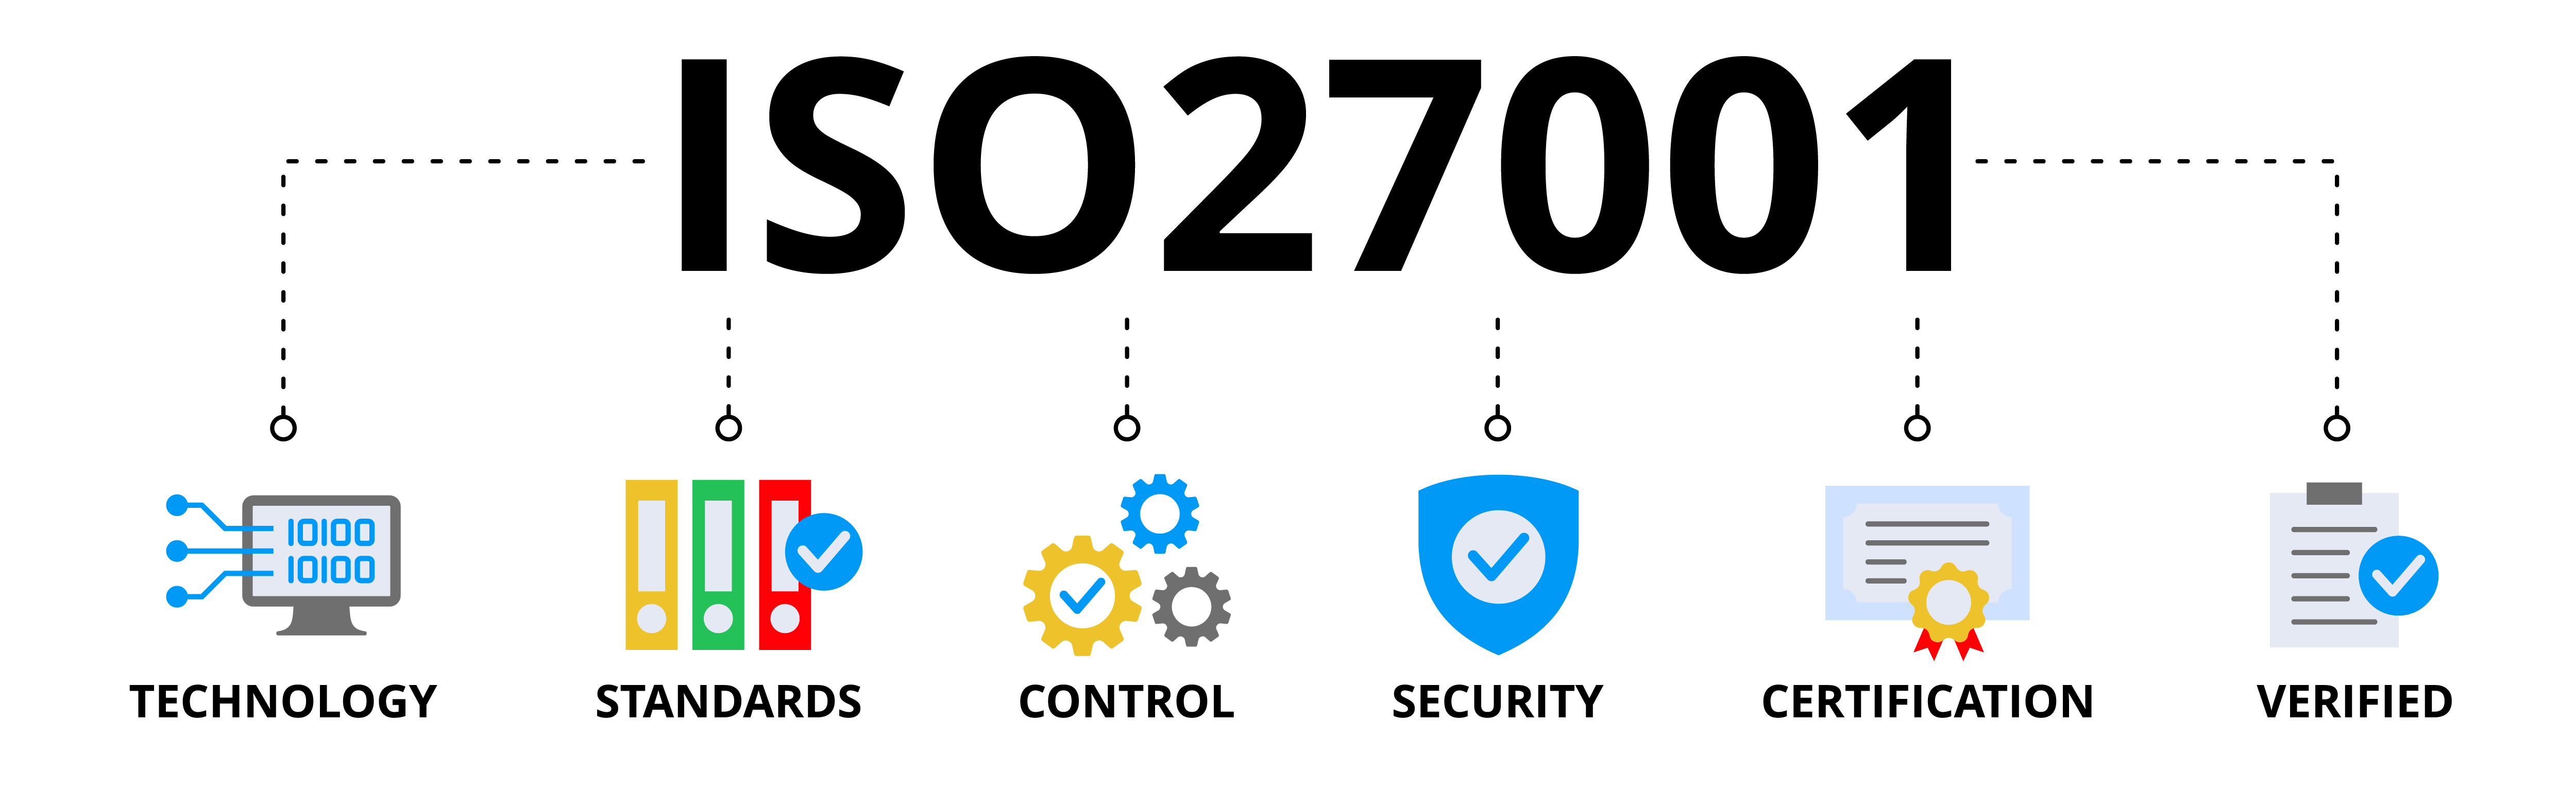
\includegraphics[width=0.6\textwidth]{img/ISO27001.png}
\caption{ISO 27001 Bilgi Güvenliği Yönetim Sistemi Standardı}
\label{fig:iso27001}
\end{figure}

ISO 27001'in en önemli özelliklerinden biri sertifikasyon sürecidir. Kuruluşlar, standartlara uygunluklarını kanıtlamak için harici bir denetçi tarafından kapsamlı bir yerinde denetime tabi tutulurlar. Denetimi geçen kuruluşlar, üç yıl geçerli olan bir ISO 27001 sertifikası alırlar. Bu sertifika, kuruluşun güvenliğe olan bağlılığını uluslararası düzeyde gösteren bir güven sinyalidir.

\subsection{NIST Cybersecurity Framework (CSF) Uygulamaları}

Ulusal Standartlar ve Teknoloji Enstitüsü (NIST) Siber Güvenlik Çerçevesi (CSF), siber güvenlik risklerini yönetmek ve azaltmak için kullanılan esnek bir rehberdir. Çerçeve, özellikle siber güvenlik programının ilk aşamalarında veya bir ihlali azaltmaya çalışırken kullanışlıdır ve daha teknik bir odak noktasına sahiptir. NIST CSF, beş ana işlevi etrafında yapılandırılmıştır:

\begin{itemize}
    \item \textbf{Tanımlama (Identify):} Sistemlerin, varlıkların, verilerin ve yeteneklerin siber güvenlik risklerini anlamak.
    \item \textbf{Koruma (Protect):} Kritik hizmetlerin sunumunu sağlamak için koruyucu önlemler almak.
    \item \textbf{Tespit Etme (Detect):} Siber güvenlik olaylarının zamanında tespit edilmesini sağlayan faaliyetleri uygulamak.
    \item \textbf{Müdahale Etme (Respond):} Bir olay tespit edildiğinde, etkilerini sınırlamak için bir plan dahilinde harekete geçmek.
    \item \textbf{Kurtarma (Recover):} Siber bir olaydan etkilenen işlevleri geri yüklemek ve iyileştirmek için planlar yapmak.
\end{itemize}

Bu beş işlev, NIST CSF'nin ana omurgasını oluşturur ve kuruluşlara risk yönetimi stratejilerini iş ihtiyaçlarıyla uyumlu hale getirme konusunda yardımcı olur.

\begin{figure}[H]
\centering
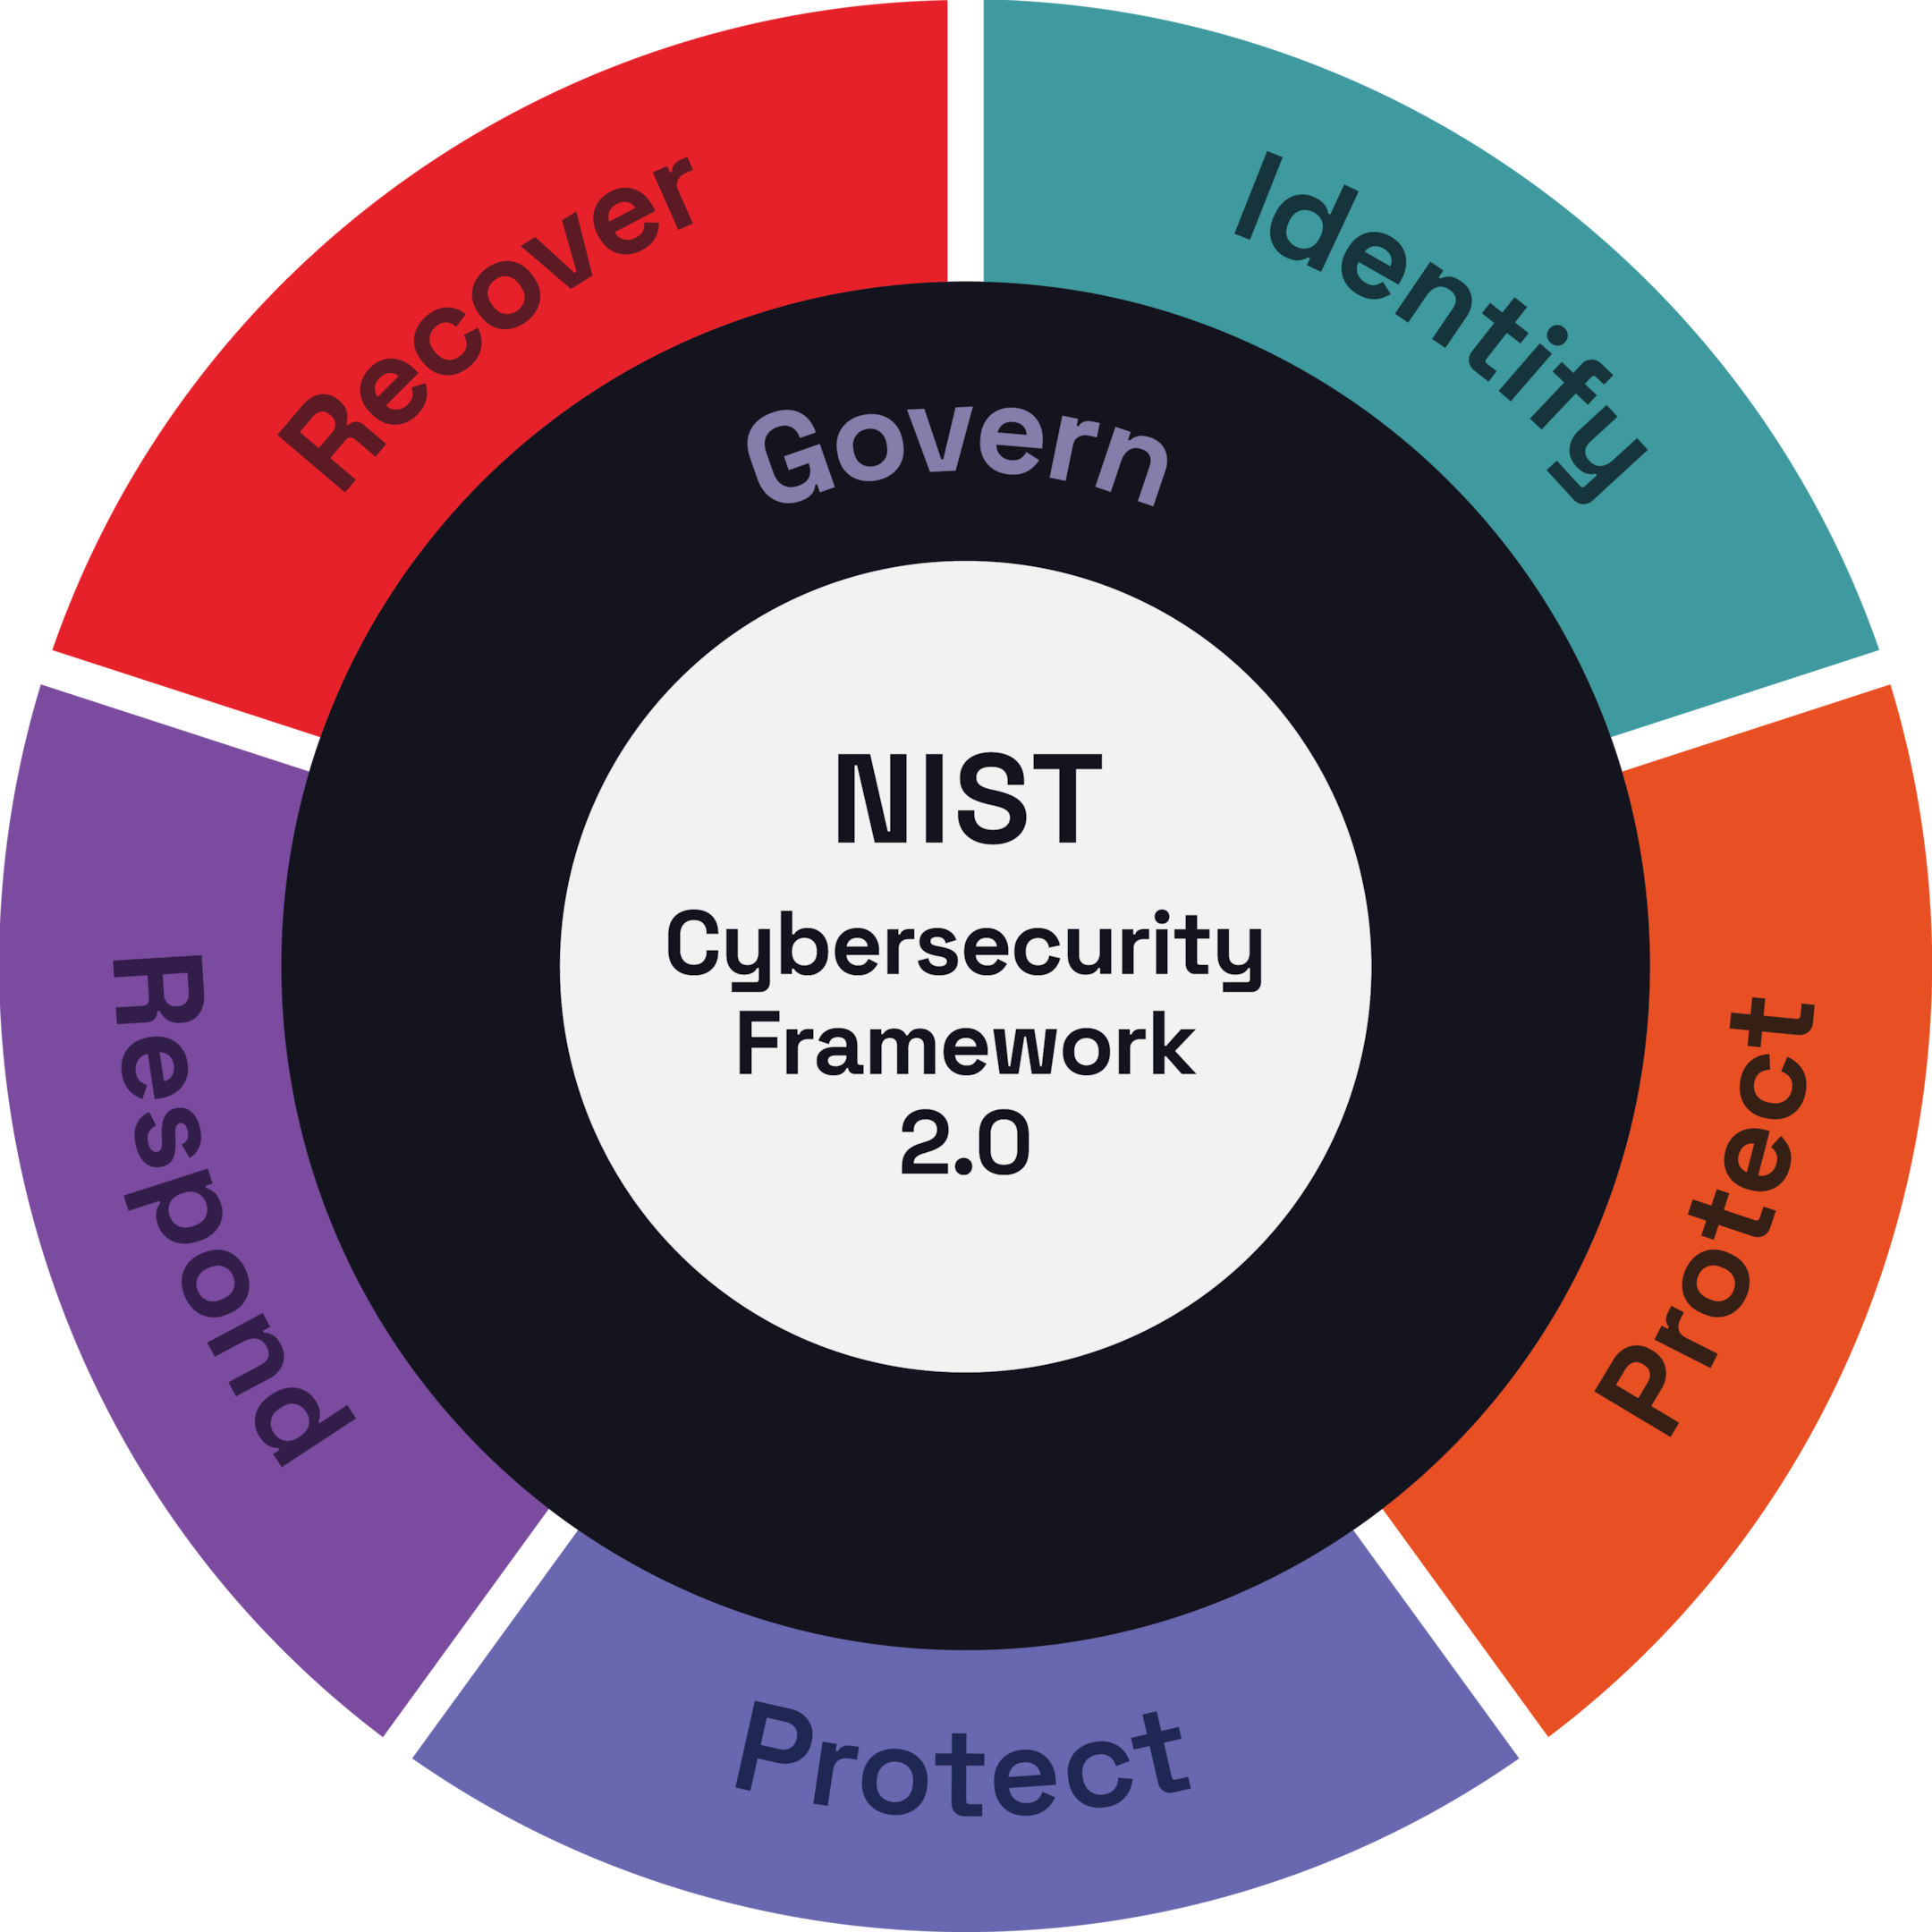
\includegraphics[width=0.8\textwidth]{img/NIST-cyber-security-framework2.0.png}
\caption{NIST Siber Güvenlik Çerçevesi 2.0 (CSF 2.0) - Altı Ana İşlev}
\label{fig:nist-csf}
\end{figure}

\textbf{ISO 27001 vs. NIST CSF Karşılaştırması}

ISO 27001 ve NIST CSF, bilgi güvenliği ve risk yönetimini farklı açılardan ele alan tamamlayıcı çerçevelerdir.

\begin{adjustbox}{max width=\textwidth}
\begin{tabularx}{\textwidth}{|l|X|X|}
\hline
\textbf{Özellik} & \textbf{ISO 27001} & \textbf{NIST CSF} \\
\hline
\textbf{Yapısı} & Bir standarttır. Uygunluğu kanıtlamak için belirli ölçütleri karşılamanız gereken bir test gibidir. & Bir rehber veya kılavuzdur. Kuruluşlara siber güvenlik programı oluşturmaları için yol gösterir. \\
\hline
\textbf{Amacı} & Mevcut bir siber güvenlik programını güçlendirmek ve standardizasyon yoluyla güven oluşturmak için idealdir. & Siber güvenlik yolculuğunun erken aşamalarında olan veya yapılandırılmış bir yaklaşım arayan kuruluşlar için en iyisidir. \\
\hline
\textbf{Kapsamı} & Uluslararası kabul görmüştür. Genellikle büyük şirketler tarafından satıcılarından istenen bir gerekliliktir. & ABD federal kurumlarına yardımcı olmak için kurulmuştur, ancak herhangi bir kuruluş tarafından kullanılabilir. Müşteriler tarafından nadiren istenen bir gerekliliktir. \\
\hline
\textbf{Maliyeti} & Üçüncü taraf denetimleri ve sertifikasyon süreci nedeniyle maliyetlidir (5.000 ila 15.000 ABD Doları veya daha fazla). & Ücretsiz erişilebilir. Üçüncü taraf denetimi veya sertifikasyon gerektirmez. \\
\hline
\textbf{Sertifikasyon} & Resmi bir denetim süreci ve sertifika gerektirir. & Resmi bir sertifika süreci yoktur. Kuruluşlar uyumluluğu kendileri rapor edebilir. \\
\hline
\end{tabularx}
\end{adjustbox}

Her iki çerçeve de benzer risk yönetimi süreçlerine dayanır ve önemli ölçüde örtüşür. Bir kuruluşa göre, NIST CSF uygulayan bir şirket, ISO 27001 uyumluluğuna \%80 oranında yaklaşmış olur ve ISO 27001 de NIST CSF yönergelerinin yarısından fazlasını içerir.

\subsection{COBIT 5 IT Governance Framework}

COBIT (Control Objectives for Information and Related Technology), Bilgi Sistemleri Denetim ve Kontrol Birliği (ISACA) tarafından geliştirilen ve BT'nin iş hedefleriyle hizalanmasını sağlamak için kullanılan bir yönetişim çerçevesidir. COBIT 5, BT'nin kurumsal hedeflere değer katmasını sağlamak için beş temel prensibe dayanır:

\begin{enumerate}
    \item \textbf{Paydaş İhtiyaçlarını Karşılama:} Çerçeve, BT'nin tüm paydaşların ihtiyaçlarını karşılayacak şekilde değer yaratmasına odaklanır.
    \item \textbf{Kuruluşu Baştan Sona Kapsama:} COBIT 5, BT yönetişimini kuruluşun tüm süreçlerine, departmanlarına ve işlevlerine entegre etmeyi hedefler.
    \item \textbf{Tek Bir Entegre Çerçeve Uygulama:} COBIT 5, diğer en iyi uygulama çerçeveleri ve standartlarla (ITIL, ISO 20000, ISO 27001 gibi) entegre çalışacak şekilde tasarlanmıştır. Bu, kuruluşların tek bir çerçeveye bağlı kalmak yerine, ihtiyaçlarına göre farklı standartların en iyi yönlerini birleştiren hibrit bir yaklaşım benimsemesini sağlar.
    \item \textbf{Bütünsel Bir Yaklaşımı Etkinleştirme:} Bu ilke, BT yönetişiminin başarıya ulaşması için sadece süreçlere değil, aynı zamanda organizasyonel yapılara, kültüre, bilgiye, hizmetlere ve insan kaynaklarına da odaklanılması gerektiğini vurgular.
    \item \textbf{Yönetişimi Yönetimden Ayırma:} COBIT, "yönetişim" (governance) ve "yönetim" (management) kavramlarını net bir şekilde ayırır. Yönetişim, paydaşların ihtiyaçlarını değerlendirme, yönlendirme ve performansı izleme ile ilgilenirken; yönetim, planlama, inşa etme, çalıştırma ve izleme ile ilgilenir.
\end{enumerate}

Bu prensipler, bir kuruluşun BT yatırımlarından beklenen değeri gerçekleştirmesine yardımcı olur. COBIT'in diğer framework'lerle entegre bir şekilde çalışmak üzere tasarlanmış olması, modern BT yönetişiminin çok boyutlu ve karmaşık doğasını yansıtan bir yaklaşımdır.

\subsection{COSO Internal Control Framework}

COSO (Committee of Sponsoring Organizations of the Treadway Commission), bir kuruluşun iç kontrol süreçlerini tasarlamasına ve uygulamasına yardımcı olan bir çerçevedir. COSO'ya göre, iç kontrol, operasyonel, finansal raporlama ve uyumluluk hedeflerine ulaşma konusunda makul bir güvence sağlamak için tasarlanmış bir süreçtir. Çerçeve, beş ana bileşenden oluşur:

\begin{enumerate}
    \item \textbf{Kontrol Ortamı (Control Environment):} Bir kuruluşun etik değerlere, dürüstlüğe ve liderlik taahhüdüne olan bağlılığını gösterir.
    \item \textbf{Risk Değerlendirmesi (Risk Assessment):} Kuruluşun hedeflerine ulaşmasını etkileyebilecek riskleri tanımlama ve analiz etme sürecidir.
    \item \textbf{Kontrol Faaliyetleri (Control Activities):} Riskleri azaltmak için tasarlanmış politikalar ve prosedürlerdir. Örneğin, erişim kontrolleri ve güvenlik politikaları bu kapsamdadır.
    \item \textbf{Bilgi ve İletişim (Information and Communication):} İç ve dış iletişim kanallarının yasal, etik ve sektörel standartlara uygun olmasını sağlar. Bu, doğru bilginin zamanında ilgili taraflara iletilmesini içerir.
    \item \textbf{İzleme (Monitoring):} Kontrollerin etkinliğinin sürekli olarak değerlendirilmesi ve gözden geçirilmesidir. Bu, dahili ve harici denetimlerle gerçekleştirilebilir.
\end{enumerate}

COSO, kuruluşların iç kontrollerini iş süreçlerine entegre etmelerini sağlayarak, yasal ve düzenleyici gerekliliklere uyumlarını kolaylaştırır.

\subsection{PCI DSS Payment Card Industry Standards}

PCI DSS (Payment Card Industry Data Security Standard), ödeme kartı verilerini (örneğin, kredi kartı bilgileri) işleyen, saklayan veya ileten tüm kuruluşlar için geçerli olan bir güvenlik standartları setidir.



\subsection{HITRUST Ortak Güvenlik Çerçevesi (CSF)}

\begin{figure}[H]
    \centering
    
\includegraphics[width=0.6\textwidth]{img/HITRUSTCSFCertifiedLogo.png}
    \caption{HITRUST CSF (Common Security Framework) Sertifikası}
    \label{fig:hitrust-csf}
\end{figure}

HITRUST CSF (Common Security Framework), özellikle sağlık sektörü için tasarlanmış kapsamlı bir güvenlik ve gizlilik çerçevesidir. Bu çerçeve, HIPAA, GDPR, ISO, NIST gibi birçok farklı standardı ve düzenlemeyi tek bir çatı altında birleştirir.

\begin{itemize}
\item \textbf{Yapı ve Bileşenler:}
\begin{itemize}
    \item 14 güvenlik kategorisi
    \item 49 kontrol alanı
    \item 156 kontrol referansı
    \item 3 olgunluk seviyesi
\end{itemize}

\item \textbf{Olgunluk Modeli:} HITRUST CSF, her kontrolün olgunluğunu 5 seviyede değerlendirir:
\begin{enumerate}
    \item Politika
    \item Prosedürler
    \item Uygulama
    \item Ölçüm
    \item Yönetim
\end{enumerate}

\item \textbf{Sertifikasyon Süreci:}
\begin{itemize}
    \item Öz-değerlendirme
    \item Doğrulanmış değerlendirme
    \item Sertifikalı değerlendirme
\end{itemize}

\item \textbf{Faydaları:}
\begin{itemize}
    \item Birden fazla düzenleme ve standardın tek bir çerçevede birleştirilmesi
    \item Risk bazlı yaklaşım
    \item Ölçeklenebilir ve özelleştirilebilir kontroller
    \item Sürekli iyileştirme modeli
\end{itemize}
\end{itemize} Standardın temel amacı, kart verilerini koruyarak dolandırıcılığı önlemektir. PCI DSS, 12 ana gereksinimden oluşur. Bu gereksinimlerden biri, kullanıcı kimliklendirmesi ve erişim kontrolü ile ilgilidir.

\textbf{Temel Gereksinimler ve Uygulama}

\begin{itemize}
    \item \textbf{Gereksinim 8: Kullanıcı Kimliklendirmesi:} Bu gereksinim, bilgisayara erişimi olan her bir kişiye benzersiz bir tanıtıcı atamasını zorunlu kılar. Ayrıca, güçlü parola politikaları gerektirir:
    \begin{itemize}
        \item Parolalar en az 90 günde bir değiştirilmelidir.
        \item Parola uzunluğu en az 7 karakter olmalıdır.
        \item Parolalar hem sayısal hem de alfabetik karakterler içermelidir.
        \item Kullanıcıların önceki dört parolasıyla aynı yeni bir parola belirlemesi engellenmelidir.
    \end{itemize}
    \item \textbf{Kapsam Belirleme:} PCI DSS uyumluluğu için, öncelikle kart verilerinin işlendiği, saklandığı veya iletildiği tüm sistemleri ve uygulamaları içeren Kart Sahibi Veri Ortamının (Card Holder Data Environment - CDE) doğru bir şekilde belirlenmesi gerekir. Bu, gereksinimlerin hangi sistemlere uygulanacağını netleştirir.
\end{itemize}

PCI DSS, kuruluşların kart verilerini korumak için teknik ve yönetsel kontrolleri uygulamalarını zorunlu kılar.

\section{Veri Sınıflandırması ve Yaşam Döngüsü Yönetimi}

Veri sınıflandırması ve yaşam döngüsü yönetimi, verilerin doğru şekilde korunmasını, yönetilmesini ve nihayetinde güvenli bir şekilde imha edilmesini sağlamak için kritik öneme sahip süreçlerdir. Bu süreçler, kuruluşların yasal düzenlemelere (örneğin GDPR veya KVKK) uymasına ve veri kaybı riskini azaltmasına yardımcı olur.

\subsection{Veri Kategorileri: Public, Internal, Confidential, Restricted}

Veri sınıflandırması, verileri hassasiyetine ve önemine göre kategorize ederek her kategoriye uygun güvenlik önlemlerinin uygulanmasını sağlar. Tipik olarak, veriler dört ana kategoriye ayrılır:

\begin{itemize}
    \item \textbf{Public (Genel):} Bu veriler, herhangi bir kısıtlama olmaksızın serbestçe kullanılabilir, yeniden kullanılabilir ve yeniden dağıtılabilir. Örnekler arasında basın bültenleri, şirket tanıtım materyalleri ve iş tanımları yer alır.
    \item \textbf{Internal (Kurum İçi):} Bu veriler yalnızca şirket personeli veya erişim yetkisi verilen çalışanlar için tasarlanmıştır. Yetkisiz ifşası genellikle büyük bir zarara yol açmaz, ancak yine de gizli tutulmalıdır. İç yazışmalar veya iş planları bu kategoriye örnek verilebilir.
    \item \textbf{Confidential (Gizli):} Gizli veriler, yetkili erişim ve özel yetkilendirme gerektirir. Bu verilerin yetkisiz ifşası veya kötüye kullanımı, şirkete önemli zararlar verebilir. Sosyal güvenlik numaraları (SSN) veya kart sahibi verileri (Cardholder Data) bu kategoride yer alır. Bu veriler, genellikle HIPAA veya PCI DSS gibi yasalarla korunur.
    \item \textbf{Restricted (Kısıtlı):} Bu, en yüksek hassasiyet seviyesine sahip veri kategorisidir. Kısıtlı verilerin yetkisiz erişimi veya ifşası, yasal suçlamalara, çok yüksek para cezalarına ve geri dönülemez itibar kaybına yol açabilir. Şirketin mülkiyetinde olan araştırma ve geliştirme verileri veya federal düzenlemelerle korunan veriler bu kategoriye girer.
\end{itemize}

\subsection{Data Ownership ve Data Stewardship Modelleri}

Veri sahipliği (Data Ownership) ve veri sorumluluğu (Data Stewardship), veri yönetişiminde iki farklı ancak birbirini tamamlayan roldür.

\begin{itemize}
    \item \textbf{Veri Sahibi (Data Owner):} Bir veri kümesi üzerinde nihai karar verme yetkisine ve hesap verebilirliğe sahip olan kişidir. Veri sahipleri, verinin nasıl kullanılacağına, erişileceğine ve saklanacağına dair politikaları ve stratejik yönü tanımlarlar. Örneğin, bir finans departmanının verilerinin sahibi genellikle CFO'dur.
    \item \textbf{Veri Sorumlusu (Data Steward):} Veri sahibinin belirlediği politikaları operasyonel düzeyde uygulayan ve günlük veri yönetimi faaliyetlerini yürüten kişidir. Veri sorumluları, veri kalitesini, tutarlılığını ve uyumluluğunu sağlamaktan sorumludur.
\end{itemize}

Aşağıdaki tablo, bu iki rol arasındaki temel farkları özetlemektedir:

\begin{tabular}{|p{3cm}|p{6.5cm}|p{6cm}|}
\hline
\textbf{Özellik} & \textbf{Veri Sahibi (Data Owner)} & \textbf{Veri Sorumlusu (Data Steward)} \\
\hline
\textbf{Yetki} & Veri kullanımı, erişimi ve saklanması hakkında nihai kararları verme yetkisi vardır. & Veri sahibinin belirlediği politikaları uygular ve operasyonel yönetimi yürütür. \\
\hline
\textbf{Odak Alanı} & Stratejik yön, risk yönetimi ve politika tanımına odaklanır. & Günlük veri kalitesini, tutarlılığını ve uyumluluğunu sağlamaya odaklanır. \\
\hline
\textbf{Sorumluluk} & Veri güvenliği politikalarını tanımlamak, riskleri yönetmek ve uyumluluğu sağlamaktan doğrudan sorumludur. & Veri kalitesini güvence altına almak, veriyi sınıflandırmak, dokümantasyon sağlamak ve uyumluluk kontrollerine yardımcı olmaktan sorumludur. \\
\hline
\end{tabular}

Veri sahipleri ve veri sorumluları, etkili bir veri yönetimi stratejisi için yakın iş birliği içinde çalışmalıdır.

\subsection{Veri Yaşam Döngüsü Yönetimi}

Veri yaşam döngüsü (Data Lifecycle), bir verinin ilk oluşturulduğu andan nihai olarak imha edildiği ana kadar geçtiği aşamalar dizisini ifade eder. Bu döngünün etkili bir şekilde yönetilmesi, verilerin güvenli, düzenlemelere uygun ve karar alma için erişilebilir kalmasını sağlar.

\textbf{Veri Yaşam Döngüsü Aşamaları:}

\begin{itemize}
    \item \textbf{Yaratma veya Edinme (Creation/Acquisition):} Veri yaşam döngüsü, verilerin müşteri etkileşimleri, işlemler, IoT cihazları veya manuel girişler gibi çeşitli kaynaklar aracılığıyla üretilmesiyle başlar. Bu aşamada, toplanan verilerin kalitesi ve alakalılığı sonraki tüm aşamalar için temel oluşturur.
    \item \textbf{Depolama (Storage):} Veriler yaratıldıktan sonra, veritabanları, veri gölleri veya bulut depolama gibi ortamlarda saklanır. Hassas bilgileri korumak ve yetkili kullanıcıların erişimini kolaylaştırmak için sağlam yedekleme ve kurtarma süreçlerinin uygulanması bu aşamada kritiktir.
    \item \textbf{Kullanım (Use):} Depolanan veriler, iş stratejilerini yönlendiren içgörüler elde etmek için analiz edilir. Veri analitiği araçları, verilerdeki kalıpları, eğilimleri ve anormallikleri ortaya çıkarmada önemli bir rol oynar. Bu aşamada, yetkisiz erişimi veya kötüye kullanımı en aza indirmek için uygun kullanım politikalarının uygulanması gerekir.
    \item \textbf{Paylaşım (Share):} Yetkili kullanıcılar veya kuruluşlar arasında veri aktarımı ve paylaşımı yapılır. Bu aşamada, gizlilik ve bütünlük ilkelerinin korunması için şifreleme ve erişim kontrolleri gibi güvenlik önlemleri uygulanmalıdır.
    \item \textbf{Arşivleme (Archive):} Veri, aktif ortamdaki kaynakları boşaltmak amacıyla daha az sıklıkta erişildiği zamanlarda güvenli, düşük maliyetli bir depolama ortamına taşınır. Bu aşama, verilerin yasal saklama süreleri dolana kadar korunmasını sağlar.
    \item \textbf{İmha (Destroy):} Döngünün son aşamasıdır ve artık gerekmeyen verilerin güvenli bir şekilde yok edilmesini içerir. Bu süreç, yasal ve düzenleyici gerekliliklere uyum sağlamak için dikkatle yönetilmelidir.
\end{itemize}

Veri yaşam döngüsü modeli, verinin durağan bir varlık olmadığını, aksine sürekli değişen bir dizi aşamadan geçtiğini gösterir. Bu, her aşama için özel güvenlik politikaları ve kontrolleri gerektirir. Örneğin, veri "kullanım" aşamasında DLP (Veri Kaybı Önleme) kontrolleri gerekirken, "imha" aşamasında güvenli silme yöntemleri (fiziksel imha, üzerine yazma) zorunlu hale gelir. Bu dinamik, statik, tek boyutlu güvenlik çözümlerinin neden yetersiz kaldığını açıklar.

\subsection{Metadata Yönetimi ve Otomatik Sınıflandırma Araçları}

Metadata, verinin içeriği hakkında bilgi sağlayan veridir (örneğin, bir dosyanın oluşturulma tarihi, sahibi veya kaynağı gibi) ve otomatik veri sınıflandırması için kritik bir unsurdur. Otomatik sınıflandırma araçları, önceden tanımlanmış kural setleri veya içerik inceleme teknikleri kullanarak belirli bir dosya veya mesajın hassasiyetini belirler ve uygun şekilde etiketler.

Otomatik sınıflandırma, ERP sistemleri tarafından üretilen raporlar gibi, kullanıcı müdahalesi olmadan oluşturulan veriler için özellikle faydalıdır. Ancak, bu araçlar her zaman verinin bağlamını anlayamayabilir ve bu da yanlış eşleşmelere veya hassas verileri kaçırmaya neden olabilir. Bu tür zorlukları aşmak için, otomasyon ile kullanıcı odaklı yaklaşımlar birleştirilebilir. Örneğin, otomatik olarak bir etiket önerisi sunularak kullanıcıdan onay istenebilir. Bu yaklaşım, sistemin doğruluğunu büyük ölçüde artırır ve kullanıcı güvenini sağlar.

Otomatik sınıflandırma araçları, DLP yazılımları ile entegre bir şekilde çalışarak, verinin hassasiyetine göre otomatik olarak kontrol edilmesini ve uygun politikanın uygulanmasını sağlar. Örneğin, "Gizli" olarak etiketlenmiş bir belgenin ağ üzerinden dışarıya aktarılması otomatik olarak engellenebilir.

\subsection{Veri Saklama ve İmha Politikaları}

Veri saklama (data retention) ve imha (disposal) politikaları, hangi verilerin ne kadar süreyle saklanacağını ve artık gerek duyulmayan verilerin nasıl güvenli bir şekilde yok edileceğini belirleyen yazılı kurallar bütünüdür. Bu politikalar, yasal ve düzenleyici gerekliliklere uyum sağlamak, depolama maliyetlerini azaltmak ve şirketi potansiyel davalardan korumak için hayati öneme sahiptir.

Veri imha yöntemleri, verilerin hassasiyetine ve ilgili mevzuat gerekliliklerine bağlı olarak seçilmelidir. Başlıca imha yöntemleri şunlardır:

\begin{enumerate}
    \item \textbf{Mantıksal Silme:} Bu yöntemler, veriyi geri getirilemez hale getirmek için yazılımsal teknikler kullanır.
    \begin{itemize}
        \item \textbf{Temizleme (Clearing):} Veri depolama cihazlarının üzerine yeni veriler yazılarak eski verilerin kurtarılmasını zorlaştıran bir tekniktir. Bu, orta düzeyde bir güvenlik sağlar.
        \item \textbf{Arındırma (Purging):} Fiziksel teknikler veya ileri teknoloji kullanarak verileri okunamaz ve laboratuvar ortamında bile kurtarılamaz hale getiren bir yöntemdir. Degaussing veya kriptografik parçalama gibi teknikler bu amaçla kullanılır.
    \end{itemize}
    \item \textbf{Fiziksel Yok Etme:} Bu yöntem, depolama ortamını tamamen yok ederek verilerin geri getirilemez hale gelmesini sağlar. Bu, hassas veriler için en yüksek güvenlik seviyesini sunar. Örnekler arasında optik veya manyetik medyanın eritilmesi, yakılması, toz haline getirilmesi veya parçalanması yer alır.
\end{enumerate}

Aşağıdaki tablo, veri imha yöntemlerini ve güvenlik seviyelerini karşılaştırmaktadır:

\begin{tabular}{|p{3.5cm}|p{5cm}|p{2.8cm}|p{4.2cm}|}
\hline
\textbf{Yöntem} & \textbf{Tanım} & \textbf{Güvenlik Seviyesi} & \textbf{Kullanım Alanı} \\
\hline
\textbf{Clearing (Temizleme)} & Verilerin üzerine yeni veriler yazılarak kurtarılmasının zorlaştırılması. & Orta & Daha az hassas veriler veya dahili kullanım için. \\
\hline
\textbf{Purging (Arındırma)} & Fiziksel teknikler veya özel algoritmalarla verilerin kurtarılamaz hale getirilmesi. & Yüksek & Hassas veriler veya regülasyonlara tabi veriler için. \\
\hline
\textbf{Physical Destruction} & Depolama cihazının eritme, yakma, parçalama gibi yöntemlerle fiziksel olarak yok edilmesi. & En Yüksek & En hassas ve yasal yükümlülük taşıyan veriler için. \\
\hline
\end{tabular}

Bu politikalar, depolama alanını boşaltmanın yanı sıra, gelecekteki operasyonlar için hayati varlıkların yanlışlıkla silinmesini de önler.

\section{Şifreleme Teknolojileri ve Anahtar Yönetimi}

Şifreleme, verileri okunamaz bir biçime dönüştürerek yetkisiz erişimi engelleyen temel bir bilgi güvenliği teknolojisidir. Bu teknolojinin doğru şekilde kullanılması, verilerin hem durağan (at rest) hem de hareket halindeyken (in transit) korunmasını sağlar.

\subsection{Simetrik ve Asimetrik Şifreleme Algoritmaları (AES, RSA, ECC)}

Şifreleme algoritmaları iki ana kategoriye ayrılır:

\begin{itemize}
    \item \textbf{Simetrik Şifreleme:} Bu yöntemde, hem şifreleme hem de şifre çözme için tek ve aynı gizli anahtar kullanılır. Yüksek performans sunduğu için büyük veri setlerinin şifrelenmesinde idealdir. \textbf{AES (Advanced Encryption Standard)}, günümüzde en yaygın kullanılan simetrik algoritmadır. Çeşitli anahtar uzunlukları (128, 192, 256 bit) sunar ve kablosuz ağ güvenliği, SSL/TLS protokolleri ve VPN'ler gibi birçok alanda kullanılır.
    \item \textbf{Asimetrik Şifreleme:} Bu yöntem, \textbf{açık anahtar} (public key) ve \textbf{özel anahtar} (private key) olmak üzere, matematiksel olarak ilişkili iki farklı anahtar kullanır. Açık anahtar herkesle paylaşılabilirken, özel anahtar yalnızca sahibinde gizli kalır. Veri açık anahtarla şifrelenir ve yalnızca ilgili özel anahtarla çözülebilir. Simetrik şifrelemeye göre daha yavaştır, bu nedenle genellikle küçük veri setlerinin (oturum anahtarları gibi) şifrelenmesi ve dijital imzalar için kullanılır.
\end{itemize}

Asimetrik şifrelemede kullanılan ana algoritmalar şunlardır:

\begin{itemize}
    \item \textbf{RSA (Rivest–Shamir–Adleman):} Güvenliği, büyük sayıları çarpanlarına ayırmanın zorluğuna dayanır. Yaygın olarak kullanılan bir algoritmadır, ancak modern tehditlere karşı daha uzun anahtar boyutları (örneğin, 2048 veya 3072 bit) gerektirebilir.
    \item \textbf{ECC (Elliptic Curve Cryptography):} RSA'ya göre daha modern ve verimli bir alternatiftir. Aynı kriptografik gücü, çok daha küçük anahtar boyutlarıyla sağlar. Bu, mobil cihazlar ve Nesnelerin İnterneti (IoT) gibi sınırlı işlem gücüne sahip ortamlar için idealdir.
\end{itemize}

Aşağıdaki tablo, bu algoritmaların teknik özelliklerini özetlemektedir:

\begin{tabular}{|p{3.5cm}|p{4cm}|p{4cm}|p{4cm}|}
\hline
\textbf{Özellik} & \textbf{Simetrik (AES)} & \textbf{Asimetrik (RSA)} & \textbf{Asimetrik (ECC)} \\
\hline
\textbf{Anahtar Sayısı} & 1 (Gizli anahtar) & 2 (Açık ve özel anahtar) & 2 (Açık ve özel anahtar) \\
\hline
\textbf{Anahtar Boyutu} & 128, 192, 256 bit & 2048, 3072, 7680 bit & 224, 256, 384 bit \\
\hline
\textbf{Performans} & Çok Hızlı & Yavaş & Daha Hızlı \\
\hline
\textbf{Temel Fonksiyon} & Toplu veri şifreleme & Dijital imza, anahtar değişimi & Dijital imza, anahtar değişimi \\
\hline
\end{tabular}

\textbf{Adım Adım Kod Örnekleri (Python)}

\textbf{Simetrik Şifreleme (AES) Örneği:}

\texttt{cryptography} kütüphanesi ile AES-GCM modunda şifreleme.

\begin{verbatim}
from cryptography.hazmat.primitives.ciphers.aead import AESGCM
import os
 
# Rastgele 256-bit anahtar ve nonce oluştur
key = os.urandom(32)
nonce = os.urandom(12)
 
# Şifrelenecek metin
plaintext = b"Gizli mesajimiz."
 
# Şifreleme işlemi
aesgcm = AESGCM(key)
ciphertext = aesgcm.encrypt(nonce, plaintext, None)
 
print(f"Şifrelenmiş metin: {ciphertext.hex()}")
 
# Şifre çözme işlemi
try:
    decrypted_text = aesgcm.decrypt(nonce, ciphertext, None)
    print(f"Şifresi çözülmüş metin: {decrypted_text.decode('utf-8')}")
except Exception as e:
    print(f"Hata: {e}")
\end{verbatim}

\textbf{Asimetrik Şifreleme (RSA) Örneği:}

\texttt{cryptography} kütüphanesi ile RSA anahtar çifti oluşturma ve şifreleme.

\begin{verbatim}
from cryptography.hazmat.primitives.asymmetric import rsa
from cryptography.hazmat.primitives import serialization
from cryptography.hazmat.primitives.asymmetric import padding
from cryptography.hazmat.primitives import hashes
 
# Özel anahtar oluşturma
private_key = rsa.generate_private_key(
    public_exponent=65537,
    key_size=2048,
)
 
# Açık anahtarı türetme
public_key = private_key.public_key()
 
# Şifrelenecek veri
message = b"Bu mesaj RSA ile sifrelenecek."
 
# Açık anahtar ile veriyi şifreleme
encrypted = public_key.encrypt(
    message,
    padding.OAEP(
        mgf=padding.MGF1(algorithm=hashes.SHA256()),
        algorithm=hashes.SHA256(),
        label=None
    )
)
 
print(f"Şifrelenmiş veri: {encrypted.hex()}")
 
# Özel anahtar ile şifre çözme
decrypted = private_key.decrypt(
    encrypted,
    padding.OAEP(
        mgf=padding.MGF1(algorithm=hashes.SHA256()),
        algorithm=hashes.SHA256(),
        label=None
    )
)
 
print(f"Şifresi çözülmüş veri: {decrypted.decode('utf-8')}")
\end{verbatim}

\subsection{Hash Fonksiyonları ve Dijital İmzalar}

Hash fonksiyonları, verinin bütünlüğünü sağlamak için kullanılan tek yönlü matematiksel algoritmalardır. Bir girdi (mesaj) ne kadar büyük olursa olsun, sabit boyutlu bir çıktı (özet veya hash değeri) üretir. Bu çıktının en önemli özelliği, girdideki en ufak bir değişikliğin bile çıktıda tamamen farklı bir değere neden olmasıdır ("çığ etkisi"). Bu tek yönlü özellik, özet değerinden orijinal verinin elde edilememesini sağlar.

Hash fonksiyonları, \textbf{dijital imza} sürecinde kritik bir rol oynar. Dijital imza, bir belgenin bütünlüğünü ve kaynağını doğrulamak için kullanılır. Eğer belgenin kendisi çok büyükse, tüm belgeyi imzalamak zaman alıcı ve kaynak yoğundur. Bunun yerine, belgenin hash değeri alınır ve bu küçük boyutlu özet değeri, göndericinin özel anahtarıyla imzalanır. Alıcı, imzalı özet değerini göndericinin açık anahtarıyla doğrulayarak mesajın bütünlüğünü kontrol eder. Bu yöntem, hem operasyonel maliyeti hem de iletişim yükünü önemli ölçüde azaltır.

\subsection{Açık Anahtar Altyapısı (PKI) ve Sertifika Yönetimi}

Açık Anahtar Altyapısı (PKI), dijital sertifikaları ve anahtar çiftlerini oluşturmak, yönetmek, dağıtmak, saklamak ve iptal etmek için gerekli olan bir dizi rol, politika, donanım, yazılım ve prosedürdür. PKI'nın temel amacı, elektronik iletişimin güvenli bir şekilde aktarılmasını sağlamak, tarafların kimliğini doğrulamak ve verinin bütünlüğünü güvence altına almaktır.

PKI'nın temel bileşenleri şunlardır:

\begin{itemize}
    \item \textbf{Sertifika Otoritesi (CA - Certificate Authority):} Güvenilir bir üçüncü taraf olan CA, dijital sertifikaları düzenler, imzalar ve iptal eder. Bir CA, kendi özel anahtarını kullanarak sertifikaları dijital olarak imzalar, böylece son kullanıcı sertifikasına olan güven, CA'nın anahtarına olan güvene dayanır.
    \item \textbf{Kayıt Otoritesi (RA - Registration Authority):} RA, bir sertifika talebinde bulunan kişinin kimliğini doğrulayan bir bileşendir. RA, talepleri alır, gerekli doğrulamaları yapar ve ardından sertifikanın düzenlenmesi için talebi CA'ya iletir. Güvenlik ve erişilebilirlik nedenleriyle RA genellikle CA'dan ayrı bir birim olarak işlev görür.
    \item \textbf{Sertifika Veritabanı:} Düzenlenen ve iptal edilen tüm sertifikaların saklandığı bir depodur.
    \item \textbf{Güven Zinciri (Chain of Trust):} Bu, bir Kök CA'dan başlayıp, ara CA'lar aracılığıyla son kullanıcı sertifikalarına kadar uzanan hiyerarşik bir yapıdır. Bir sertifikanın doğruluğu, zincirdeki her bir sertifikanın bir üst otorite tarafından imzalanmış olmasıyla doğrulanır. Bu zincir, bir sertifikanın geçerliliğini kontrol etmek için kritik bir rol oynar.
\end{itemize}

\subsection{Donanım Güvenlik Modülleri (HSM) ve Anahtar Yönetim Sistemleri (KMS)}

Anahtar yönetimi, şifreleme teknolojilerinin güvenli bir şekilde uygulanabilmesi için hayati önem taşır. Bu alanda iki temel teknoloji öne çıkar: Donanım Güvenlik Modülleri (HSM) ve Anahtar Yönetim Sistemleri (KMS).

\begin{itemize}
    \item \textbf{Donanım Güvenlik Modülü (HSM):} Bir HSM, şifreleme anahtarlarını fiziksel olarak koruyan, kurcalamaya dayanıklı bir donanım cihazıdır. Bir "banka kasası"na benzetilebilir; anahtarlar HSM içinde oluşturulur, depolanır ve imha edilir ve bu cihazdan asla çıkarılamaz. FIPS 140-2 Seviye 3 gibi düzenleyici standartlara uygun olan HSM'ler, fiziksel bir saldırı durumunda anahtarları otomatik olarak yok etme yeteneğine sahiptir. Bu özelliği, onları bir "Güvenin Kökü" (Root of Trust) olarak işlev görmesi gereken kritik altyapılarda vazgeçilmez kılar.
    \item \textbf{Anahtar Yönetim Sistemi (KMS):} KMS, şifreleme anahtarlarının yaşam döngüsünü (oluşturma, rotasyon, dağıtım, depolama ve imha) büyük ölçekte yönetmeye odaklanan bir yazılım çözümüdür. KMS, erişim politikalarını uygulamayı, kullanımı izlemeyi ve denetim kayıtları tutmayı kolaylaştırır.
\end{itemize}

Sadece birini kullanmak, güvenlikte önemli boşluklar yaratabilir. Sadece KMS kullanmak "uygun ama riskli" olabilir, çünkü anahtarlar yazılımda depolandığından yanlış bir yapılandırma veya bir zafiyet nedeniyle ifşa olma riski taşır. Sadece HSM kullanmak ise "güvenli ama yönetimi zor"dur, çünkü geniş ölçekte politika uygulamayı ve anahtar rotasyonunu manuel hale getirir. Optimal çözüm, her iki teknolojinin birlikte kullanıldığı hibrit bir modeldir. Bu modelde, KMS yönetim ve ölçeklenebilirlik sağlar, HSM ise anahtarlar için en yüksek düzeyde fiziksel korumayı sunar.

\begin{adjustbox}{max width=\textwidth}
\begin{tabularx}{\textwidth}{|l|X|X|X|}
\hline
\textbf{Özellik} & \textbf{Sadece HSM} & \textbf{Sadece KMS} & \textbf{KMS + HSM Birlikte Kullanımı} \\
\hline
\textbf{Anahtarın Depolandığı Yer} & Fiziksel bir donanım cihazı içinde. & Genellikle yazılım veya sanal makine içinde. & Anahtarlar HSM'de güvenli bir şekilde depolanır, ancak KMS üzerinden yönetilir. \\
\hline
\textbf{Güvenlik Riski} & Fiziksel olarak güvenlidir, ancak ölçeklenebilirlik ve yönetim eksikliği riskleri barındırır. & Kullanışlıdır, ancak yanlış yapılandırma veya zafiyetler anahtarları ifşa edebilir. & Anahtarlar güvende kalır ve kolayca yönetilebilir. \\
\hline
\textbf{Kontrol \& Yönetim} & Manuel operasyonlar gerektirir; politika uygulaması ve izleme zordur. & Kuralları belirlemek, anahtarları döndürmek ve kullanımı günlüğe kaydetmek kolaydır. & Politikaları belirlemek, izlemek ve otomatikleştirmek için güçlü bir koruma katmanı mevcuttur. \\
\hline
\textbf{Uyum Hazırlığı} & Yeterli değildir; politika kontrolü ve denetlenebilirlik eksiktir. & Yetersizdir; "güvenin kökü" eksiktir. & Entegre politika kontrolü ve donanım koruması sayesinde tam uyumluluk sağlar. \\
\hline
\end{tabularx}
\end{adjustbox}

Bu yaklaşım, siber güvenlikte "tek bir çözüm her derde deva olmaz" prensibinin bir kanıtıdır. En yüksek güvenliğin, farklı teknolojilerin en iyi yönlerini birleştiren katmanlı ve entegre çözümlerle elde edildiğini gösterir.

\subsection{Kuantum-Güvenli Kriptografi ve Post-Kuantum Algoritmaları}

Kuantum bilgisayarlar, mevcut şifreleme yöntemlerinin güvenliğini tehdit eden yeni bir risk alanıdır. Shor's algoritması gibi kuantum algoritmaları, günümüzün yaygın asimetrik şifreleme algoritmalarının (örneğin RSA) dayandığı matematiksel problemleri (büyük sayıları çarpanlarına ayırma) çözme potansiyeline sahiptir. Grover's algoritması ise simetrik algoritmaların (AES gibi) kaba kuvvet saldırılarına karşı direncini azaltabilir, ancak bu algoritmalara karşı korunmak genellikle anahtar boyutunu iki katına çıkarmakla mümkün olabilir.

\textbf{Kuantum-Güvenli Kriptografi (PQC)}, standart bilgisayarlarda çalışabilen ancak kuantum bilgisayarların saldırılarına karşı dirençli olan yeni algoritmaların geliştirilmesidir. Bu algoritmalar, kuantum bilgisayarların çözemeyeceği varsayılan matematiksel problemlere (örneğin, kafes tabanlı kriptografi) dayanır.

NIST, kuantum-güvenli kriptografi için yeni standartlar belirlemek amacıyla bir yarışma başlatmıştır. Bu süreç sonucunda \textbf{CRYSTALS-Kyber} (şifreleme) ve \textbf{CRYSTALS-Dilithium} (dijital imzalar) algoritmaları birincil standartlar olarak seçilmiştir. Bu algoritmalar, yüksek güvenlik sunmanın yanı sıra, dengeli anahtar boyutları ve güçlü performans özelliklerine sahiptir.

\section{Veri Kaybı Önleme (DLP) ve Veri Koruma Teknolojileri}

Veri Kaybı Önleme (DLP), hassas verilerin yetkisiz kişilere ifşasını, aktarımını veya sızdırılmasını tespit eden, önleyen ve yöneten bir dizi araç ve süreçtir. DLP çözümleri, bir kuruluşun fikri mülkiyetini, kişisel olarak tanımlanabilir bilgilerini (PII) korumasına ve dijital gizlilik yasalarına uymasına yardımcı olur.

\begin{figure}[H]
    \centering
    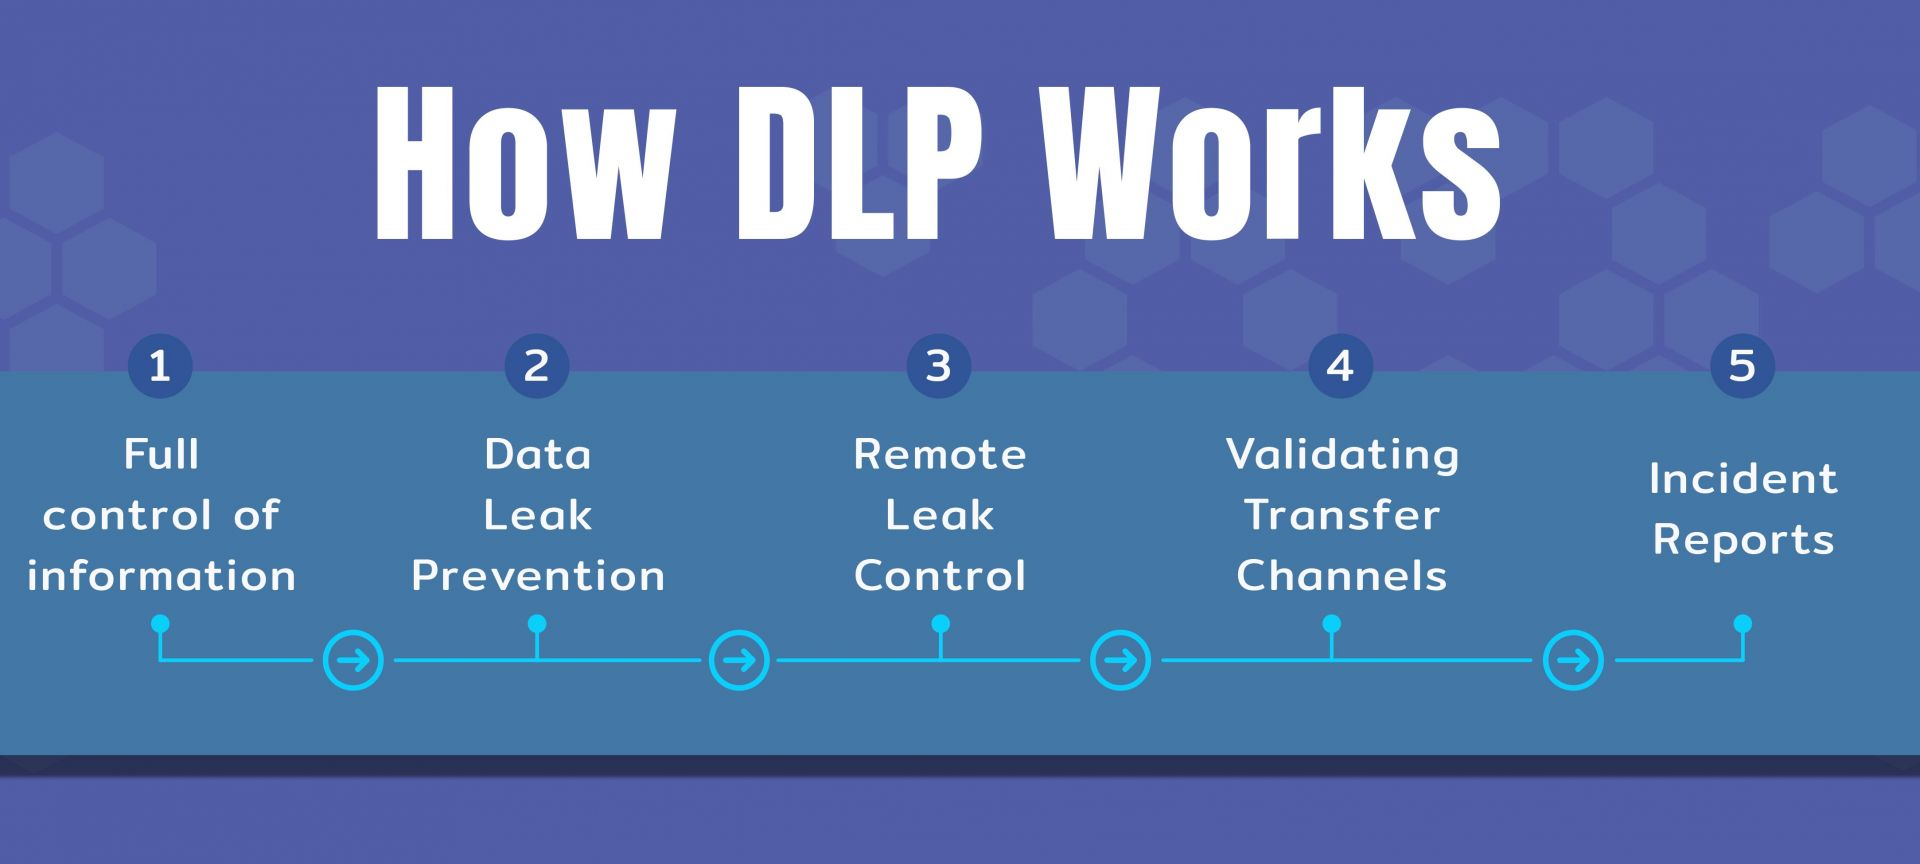
\includegraphics[width=0.8\textwidth]{img/dlp.png}
    \caption{Veri Kaybı Önleme (DLP) Teknolojileri ve Mimarisi}
    \label{fig:dlp}
\end{figure}

\subsection{Ağ Tabanlı, Uç Nokta Tabanlı ve Depolama Tabanlı DLP}

DLP çözümleri, odaklandıkları koruma alanına göre üç ana türe ayrılır:

\begin{itemize}
    \item \textbf{Ağ Tabanlı (Network-based) DLP:} Ağ trafiğini gerçek zamanlı olarak izler ve hassas verilerin e-posta veya diğer ağ protokolleri aracılığıyla yetkisiz bir şekilde dışarı aktarılmasını engeller. Geleneksel olarak, tüm çalışanların ofis ağına bağlı olduğu ve trafiğin merkezileştirildiği on-premise (yerinde) ortamlarda temel bir bileşendi. Ancak, uzaktan çalışma ve bulut tabanlı mimarilerin yaygınlaşmasıyla, ağ tabanlı DLP'nin etkinliği azalmıştır, çünkü ağın dışındaki etkinlikleri veya bulut uygulamaları arasındaki veri akışını izleyemez.
    \item \textbf{Uç Nokta Tabanlı (Endpoint-based) DLP:} Dizüstü bilgisayarlar, masaüstü bilgisayarlar ve mobil cihazlar gibi bireysel uç noktalardaki verileri kontrol eder. Bu çözümler, verilerin kaynağında nasıl kopyalandığını, taşındığını, yüklendiğini veya paylaşıldığını izler ve engeller. Kullanıcı ağa bağlı olmasa bile çalışır ve bu nedenle uzaktan çalışmanın yaygın olduğu günümüz ortamında vazgeçilmez bir çözüm haline gelmiştir.
    \item \textbf{Depolama Tabanlı (Storage-based) DLP:} Veritabanları, dosya sunucuları ve bulut depoları gibi "durağan" haldeki verileri tarar. Bu çözümler, hassas verileri keşfeder, sınıflandırır ve uygun koruma önlemlerini (örneğin, şifreleme) uygular.
\end{itemize}

Uzaktan çalışmanın yaygınlaşmasıyla birlikte, veri güvenliğinin odak noktası ağ çevresinden, verinin asıl bulunduğu yer olan uç noktalara kaymıştır. Bu, güvenlik teknolojilerinin, iş yapış biçimlerindeki köklü değişikliklere nasıl yanıt verdiğinin somut bir örneğidir. Modern bir DLP stratejisi, uç nokta tabanlı çözümlerin temel bir bileşen olmasını gerektirir.

\subsection{İçerik İnceleme (Content Inspection) ve Örüntü Eşleştirme (Pattern Matching) Teknikleri}

İçerik İnceleme, DLP çözümlerinin hassas verileri tanımlamak için veri paketlerinin içeriğini analiz ettiği bir tekniktir. Bu süreç, hassasiyet belirten anahtar kelimeleri ("gizli" gibi) ve belirli yapıları arar. İçerik incelemenin temelinde yatan en güçlü tekniklerden biri de \textbf{Örüntü Eşleştirme (Pattern Matching)}'dir. Bu teknik, daha büyük bir metin içinde belirli karakter dizilerini veya kalıpları tanımlamayı içerir ve genellikle \textbf{Düzenli İfadeler (Regular Expressions - Regex)} kullanılarak uygulanır.

\textbf{Pratik Örnekler: Hassas Veri için Düzenli İfadeler (Regex)}

DLP politikaları, finansal veriler, kişisel kimlik bilgileri veya sağlık bilgileri gibi hassas verileri tespit etmek için regex desenlerini kullanır.

\begin{itemize}
    \item \textbf{Kredi Kartı Numarası Eşleştirme (MasterCard Örneği):} \\
    MasterCard numaraları genellikle 51 ile 55 arasında başlayan 16 haneli sayılardır. Metin içinde çeşitli formatlarda (boşluklu, tireli, vb.) yazılabilen bu numaraları tespit etmek için karmaşık regex desenleri kullanılır.
    \begin{itemize}
        \item \texttt{5[1-5][0-9]\{14\}}: Bu desen, 5 ile başlayan, ikinci hanesi 1-5 arasında olan ve toplamda 16 haneli düz bir sayı dizisini eşleştirir.
        \item \texttt{(5[1-5][0-9]\{14\}|222[1-9]|22[3-9][0-9]|2[3-6][0-9]\{2\}|27[0-9]|2720)[0-9]\{12\}}: Bu daha kapsamlı bir ifadedir ve MasterCard'ın yeni numaralandırma aralıklarını da kapsar.
    \end{itemize}

    \item \textbf{TC Kimlik Numarası Eşleştirme:} \\
    Türkiye Cumhuriyeti Kimlik Numarası (TCKN), 11 haneli bir sayıdır ve belirli kurallara uyar.
    \begin{itemize}
        \item Regex deseni: \texttt{\textasciicircum[1-9]\{1\}[0-9]\{9\}[0-9]\{1\}\textdollar}
        \item \textbf{Mantık:}
        \begin{itemize}
            \item \texttt{\textasciicircum}: İfadenin başında olduğunu belirtir.
            \item \texttt{[1-9]\{1\}}: İlk hane 0 olamaz. 1 ile 9 arasında tek bir rakamdır.
            \item \texttt{[0-9]\{9\}}: Sonraki dokuz hane 0 ile 9 arasında herhangi bir rakam olabilir.
            \item \texttt{[0-9]\{1\}}: Son hane de bir rakam olmalıdır.
            \item \texttt{\textdollar}: İfadenin sonunda olduğunu belirtir.
        \end{itemize}
    \end{itemize}
\end{itemize}



Bu basit örnekler, DLP'nin hassas verileri otomatik olarak nasıl tanımlayabildiğini ve kurum politikalarını uygulayabildiğini gösterir.

\subsection{Veri Sınıflandırma Entegrasyonu ve Politika Uygulama}

DLP çözümleri, otomatik veri sınıflandırma araçlarıyla entegre çalışarak, bir verinin hassasiyet seviyesini temel alarak politika uygulaması yapar. Bu entegrasyon, bir verinin (örneğin bir Word belgesi veya e-posta) sınıflandırma etiketi ile işaretlenmesini ve bu etikete göre DLP'nin uygun kontrolü uygulamasını sağlar. Örneğin, bir belge "Gizli" olarak etiketlendiğinde, DLP politikası bu belgenin ağ üzerinden e-posta ile gönderilmesini veya USB diske kopyalanmasını otomatik olarak engelleyebilir. Bu, güvenlik politikalarının verinin kendisiyle ilişkilendirilmesini ve yetkisiz veri aktarımlarının gerçek zamanlı olarak önlenmesini sağlar.

\subsection{Bulut DLP ve Çoklu Bulut Veri Koruma Stratejileri}

Bulut Veri Kaybı Önleme (Cloud DLP), bir kuruluşun bulut depolama hizmetleri, veritabanları ve uygulamaları içindeki hassas verileri korumaya odaklanan bir veri güvenliği stratejisidir. Bulut ve çoklu bulut ortamlarının karmaşıklığı ve ölçeği, DLP'nin manuel olarak yönetilmesini zorlaştırır. Bu nedenle, bulut DLP çözümleri genellikle otomasyon ve yapay zeka (AI) araçlarını kullanır.

Bulut DLP stratejisinin temel adımları şunlardır:

\begin{enumerate}
    \item \textbf{Veri Keşfi (Data Discovery):} Kuruluşun bulut altyapısı taranarak (örneğin, S3 depolama kovalıkları veya bulut veritabanları) PII, finansal kayıtlar veya fikri mülkiyet gibi hassas veriler keşfedilir.
    \item \textbf{Veri Sınıflandırması (Data Classification):} Keşfedilen hassas veriler, önceden tanımlanmış kurallar ve politikalar doğrultusunda Public, Confidential, Restricted gibi kategorilere ayrılır.
    \item \textbf{Politika Uygulama (Policy Enforcement):} Potansiyel bir politika ihlali tespit edildiğinde, bulut DLP çözümü, veri aktarımını engellemek, veriyi şifrelemek veya anonimleştirmek gibi önceden tanımlanmış eylemleri gerçekleştirir.
\end{enumerate}

Manuel DLP süreçleri, geniş ve dinamik bulut ortamlarında yorucu ve hataya açık olabilir. Bu nedenle, otomasyon ve yapay zeka, bulut güvenliğinde sadece bir kolaylık değil, operasyonel bir zorunluluk haline gelmiştir. Otomasyon, insan hatasını en aza indirerek ve idari yükü azaltarak uzmanların daha stratejik görevlere odaklanmasını sağlar.

\subsection{Veri Maskeleme (Data Masking) ve Anonimleştirme Teknikleri}

Veri Maskeleme ve Anonimleştirme, hassas verilerin gizliliğini korumak için kullanılan tekniklerdir.

\begin{itemize}
    \item \textbf{Veri Maskeleme:} Gerçek verinin, gerçek görünümlü ancak sahte verilerle değiştirilmesi işlemidir. Bu teknik, genellikle geliştirme, test veya analiz ortamlarında gerçek verilerin gizliliğini tehlikeye atmadan iş süreçlerinin devamını sağlamak için kullanılır. Örneğin, bir kullanıcının adı ve soyadı "J*** S****" gibi maskelenebilir.
    \item \textbf{Anonimleştirme:} Bir verinin, bir kişiyle ilişkilendirilemeyecek hale getirilmesi işlemidir. Kişisel Verilerin Korunması Kanunu'na (KVKK) göre, kişisel verinin kimliği belirlenebilir bir gerçek kişiyle ilişkilendirilemeyecek hale getirilmesi, bu verinin kişisel veri statüsünden çıkmasını sağlar.
\end{itemize}

\textbf{Pratik Anonimleştirme Örnekleri:}

\begin{itemize}
    \item \textbf{Genelleştirme:} Verilerin daha genel bir kapsama indirgenmesidir. Örneğin, çalışanların tek tek yaşlarını belirtmek yerine, "X yaşında Z kadar çalışan bulunmaktadır" şeklinde genel bir ifade kullanılabilir.
    \item \textbf{Alt ve Üst Sınır Kodlama:} Verilerin önceden tanımlanmış kategorilere göre birleştirilmesidir. Örneğin, çalışanların kıdem yıllarını "5 yıldan az", "5 ile 10 yıl arasında" veya "10 yıldan çok" olarak anonim hale getirmek.
    \item \textbf{Değişken Çıkarma:} Veri setinden doğrudan kimlik belirleyici olan "Ad", "Soyad", "Adres" gibi değişkenlerin çıkarılması.
\end{itemize}

Veri imhası için ise, mantıksal veya fiziksel yok etme yöntemleri kullanılır. Örneğin, optik medyanın eritilmesi veya yakılması gibi fiziksel işlemler verilerin geri getirilemez hale gelmesini sağlar.

\section{Uyum (Compliance) ve Düzenleyici Çerçeveler}

Siber güvenlik politikaları, giderek artan bir şekilde yasal ve düzenleyici çerçeveler tarafından şekillendirilmektedir. Bu çerçeveler, kuruluşlara veri güvenliğini sağlama ve ihlallere karşı önlem alma konusunda yasal yükümlülükler getirir.

\subsection{GDPR (General Data Protection Regulation) ve Tasarımla Gizlilik (Privacy by Design)}

Genel Veri Koruma Tüzüğü (GDPR), Avrupa Birliği'nde kişisel verilerin korunmasını düzenleyen kapsamlı bir yasadır. GDPR, veri işlemeye yönelik temel ilkeleri belirler: hukuka uygunluk, dürüstlük, şeffaflık, amaç sınırlaması ve veri minimizasyonu.

GDPR'ın en önemli ilkelerinden biri, \textbf{Tasarımla Gizlilik (Privacy by Design)} kavramıdır. Bu ilke, gizliliğin bir ürünün veya sistemin tasarımının en başından itibaren düşünülmesi ve güvenlik önlemlerinin varsayılan olarak entegre edilmesi gerektiğini belirtir. Bu, gizliliğin sonradan eklenen bir özellik değil, temel bir mimari bileşen olmasını zorunlu kılar.

\subsection{KVKK (Kişisel Verilerin Korunması Kanunu) Uygulamaları}

Türkiye'de kişisel verilerin korunması, 6698 sayılı Kişisel Verilerin Korunması Kanunu (KVKK) ile düzenlenmiştir. KVKK, GDPR ile benzer ilkeleri benimsemekle birlikte, bazı önemli farklar bulunmaktadır.

\begin{itemize}
    \item \textbf{Rıza Şartları:} KVKK, kişisel verilerin açık rıza olmadan işlenmesini genel bir kural olarak yasaklar ve belirli sınırlı durumlarda istisnalara izin verir. GDPR ise veri işlemeye yönelik rıza dışında daha geniş yasal zeminler (sözleşme, yasal yükümlülük, meşru menfaat gibi) sunar.
    \item \textbf{Hesap Verebilirlik:} GDPR, veri sorumlularının veri işleme faaliyetlerinin kanuna uygunluğunu ispatlamakla yükümlü olduğunu açıkça belirtir. KVKK'da bu ilke açıkça belirtilmemiştir, ancak veri sorumlularının kişisel verilerin güvenliğini sağlamak için gerekli önlemleri alma yükümlülüğü bu kavramı dolaylı olarak içerir.
\end{itemize}

\subsection{HIPAA Sağlık Bilgileri Gizliliği}

Sağlık Sigortası Taşınabilirlik ve Sorumluluk Yasası (HIPAA), ABD'deki sağlık kuruluşları ve iş ortakları tarafından hasta bilgilerinin (Korunan Sağlık Bilgisi - PHI) gizliliğini ve güvenliğini korumayı hedefler. HIPAA, sağlık verilerinin toplanmasını, kullanılmasını ve ifşa edilmesini düzenleyen katı kurallar içerir.

HIPAA, okullardaki öğrenci sağlık kayıtları söz konusu olduğunda genellikle Aile Eğitimi Hakları ve Gizlilik Yasası (FERPA) ile birlikte değerlendirilir. Bir öğrencinin sağlık kayıtları, eğer okul tarafından tutuluyorsa, genellikle HIPAA değil, FERPA kapsamında yer alır.

\subsection{SOX (Sarbanes-Oxley) Finansal Veri Koruması}

Sarbanes-Oxley Yasası (SOX), halka açık şirketlerin finansal raporlamalarını ve iç denetim mekanizmalarını düzenleyen bir ABD yasasıdır. SOX, BT altyapılarında iç dolandırıcılığı önlemeye yönelik katı iç denetim ve erişim kontrolü gereklilikleri getirmiştir. SOX uyumluluğu, kullanıcı hesaplarına erişimin izlenmesini ve hassas sistemlerdeki aktivitelerin denetlenmesini zorunlu kılar.

\subsection{Türkiye Siber Güvenlik Kanunu ve İşletmelere Etkileri}

Mart 2025 itibarıyla yürürlüğe giren Türkiye Siber Güvenlik Kanunu, ülkenin dijital güvenliğini güçlendirmeyi ve siber tehditlere karşı daha dirençli bir altyapı oluşturmayı hedefler. Kanun, yalnızca kamu kurumlarını değil, kritik altyapı olarak tanımlanan finans, sağlık, enerji, ulaştırma ve telekomünikasyon gibi özel sektör kuruluşlarını da doğrudan etkilemektedir.

Bu kanun, işletmelere bir dizi yeni yükümlülük getirmektedir:

\begin{itemize}
    \item \textbf{Siber Güvenlik Sorumlusu Atama Zorunluluğu:} 50'den fazla çalışanı olan özel şirketler ve kamu kurumları, organizasyon yapısı içinde bir siber güvenlik sorumlusu veya birimi oluşturmakla yükümlüdür.
    \item \textbf{Olay Bildirim Süresi:} Siber güvenlik olaylarının, olayın tespit edilmesini takiben 48 saat içinde ilgili birimlere bildirilmesi zorunludur.
    \item \textbf{Zorunlu Teknik Önlemler:} İşletmelerin güçlü kimlik doğrulama sistemleri, sızma testleri (penetration test), güncel antivirüs ve güvenlik duvarları gibi temel teknik tedbirleri alması zorunluluk haline gelmiştir.
    \item \textbf{Bağımsız Denetim:} Kritik altyapı sağlayıcıları, yılda en az bir kez bağımsız siber güvenlik denetimine tabi tutulacak ve bu denetim sonucunda "Siber Güvenlik Uygunluk Sertifikası" alacaktır.
    \item \textbf{Cezai Yaptırımlar:} Yükümlülüklere uymayan şirketlere ciddi idari para cezaları uygulanabilir (brüt satış gelirinin \%5'ine kadar). Siber güvenlikle ilgili yanlış bilgi yayarak kamuoyunda panik yaratanlar için 2 ila 5 yıl arasında hapis cezası öngörülmüştür.
\end{itemize}

Bu kanun, siber güvenliği "tercih edilebilir bir iyileştirme" olmaktan çıkarıp, uyulması zorunlu ve ciddi yaptırımları olan bir hukuki yükümlülük haline getirmiştir. Bu durum, siber güvenlik politikalarının ve yatırımlarının üst düzey yönetim tarafından stratejik bir öncelik olarak ele alınmasını gerektirir. Kanun, sadece teknolojik çözümlerin değil, aynı zamanda kurumsal farkındalığın, risk yönetiminin ve sürekli denetimin de zorunlu hale geldiği yeni bir dönemi başlatır. Bu, regülasyonların teknolojik ve yönetsel dönüşümü nasıl tetiklediğinin önemli bir göstergesidir.
\chapter{AĞ GÜVENLİĞİ MİMARİSİ VE ALTYAPI KORUMA}

Bu kapsamlı eğitim belgesi, siber güvenlik alanındaki uzmanlar için tasarlanmıştır ve modern ağ güvenliği mimarilerinin temelini oluşturan prensipleri, teknolojileri ve pratik uygulamaları detaylandırmaktadır. Bu bölüm, ağ altyapısının korunması için hem teorik hem de uygulamalı bir çerçeve sunmaktadır.

\section{Ağ Güvenlik Mimarisi ve Tasarım Prensipleri}

Modern ağ güvenliği, tek bir savunma hattına dayanmaktan ziyade, stratejik olarak katmanlanmış ve birbirini tamamlayan mekanizmalarla oluşturulan sağlam bir mimariyi gerektirir. Bu yaklaşım, bir siber saldırganın ağa erişimini zorlaştırmak, ihlalin etki alanını sınırlamak ve tespit edilme şansını artırmak için tasarlanmıştır.

\subsection{Defense-in-Depth Network Architecture (Katmanlı Savunma Ağ Mimarisi)}

Defense-in-Depth (DiD), bir bilgi güvenliği felsefesidir ve bir ağdaki gizlilik, bütünlük ve erişilebilirliği korumak için bir dizi güvenlik mekanizmasının ve kontrolünün katmanlar halinde yerleştirilmesini ifade eder. Hiçbir bireysel önlem tüm siber tehditleri durduramaz, ancak birlikte çalışarak çok çeşitli tehdit vektörlerine karşı koruma sağlarlar ve bir mekanizma başarısız olduğunda yedeklilik sunarlar. Bu strateji başarılı olduğunda, ağın güvenliğini birçok farklı saldırı vektörüne karşı önemli ölçüde güçlendirir.
Bu katmanlı yaklaşım, bir ağda birden fazla güvenlik kontrolünün stratejik olarak konumlandırılmasını içerir. Bu katmanlar, geleneksel ağ güvenlik duvarlarından (firewalls), kötü niyetli trafiği tespit edip engelleyen Saldırı Tespit ve Önleme Sistemlerine (IDS/IPS) kadar uzanır. Ayrıca, kullanıcıların dizüstü bilgisayarları veya mobil cihazları gibi uç noktalara yerleştirilen antivirüs koruması, tehdit tespiti ve analizi sağlayan Uç Nokta Tespit ve Yanıt (EDR) yazılımlarını da kapsar. Temel bir adım olan ağ segmentasyonu, ağı iş ihtiyaçlarına göre alt ağlara ayırarak yanal hareketin önlenmesine yardımcı olurken, Çok Faktörlü Kimlik Doğrulama (MFA) ve şifreleme gibi önlemler, kullanıcı ve veri düzeyinde koruma sağlar.
Bu güvenlik felsefesinin altında yatan temel mantık, siber güvenlikte "tek bir gümüş kurşun"un olmadığıdır. Bir saldırgan, bir katmanı aşsa bile, bir sonraki katmanla karşılaşır. Bu durum, başarılı bir ağ ihlali için gereken süreyi ve karmaşıklığı artırır, böylece aktif bir saldırının tamamlanmadan önce tespit edilme ve durdurulma olasılığını yükseltir. Bu katmanlı savunma yaklaşımı, fiziksel güvenlikte de rutin olarak uygulanmaktadır. Örneğin, değerli varlıkları korumak için güvenlik kameraları, kurşun geçirmez cam ve kasaların kullanılması, aynı prensibin somut bir örneğidir. Bu paralellik, siber güvenlik uzmanlarının hem dijital hem de fiziksel güvenlik problemlerinin temelinde yatan ortak mantığı anlaması gerektiğini göstermektedir. Bir ağın savunmasını, bir kalenin kapıları, duvarları ve hendekleri gibi katman katman korumaya benzetmek, sadece bir ağa rastgele güvenlik araçları eklemekten daha fazlası olduğunu, bir güvenlik mimarisi oluşturma yaklaşımı olduğunu vurgular.

\subsection{Network Segmentation ve Micro-segmentation Stratejileri}

Ağ segmentasyonu, bir ağı daha küçük, izole edilmiş segmentlere ayırma uygulamasıdır ve siber güvenlik riskini azaltmanın hayati bir adımıdır. Mikro-segmentasyon ise bu yaklaşımın daha granüler bir formudur; ağı iş yükleri, uygulamalar ve hatta bireysel cihazlar düzeyinde izole eder. Bu strateji, bir saldırganın ağa ilk erişimi sağladıktan sonra yanal hareketini (lateral movement) zorlaştırarak bir ihlalin etki alanını ("blast radius") sınırlar ve genel saldırı yüzeyini azaltır.
Bu stratejiyi başarılı bir şekilde uygulamak, metodolojik bir süreç gerektirir:

\begin{enumerate}
\item \textbf{Değerli Veri ve Varlıkları Tanımlama:} Bir kuruluştaki tüm veri ve varlıklar aynı değere sahip değildir. Müşteri veritabanı gibi operasyonlar için hayati olan sistemlerin belirlenmesi ilk adımdır.
\item \textbf{Sınıflandırma Etiketleri Atama:} Hassasiyet seviyelerine göre varlıklara etiketler atayın (örneğin, "Gizli," "Özel"). Bu etiketler, daha sonra ağ içindeki güven bölgelerini tanımlamak için kullanılır.
\item \textbf{Veri Akışlarını Haritalama:} Ağ genelindeki veri akışlarını haritalayarak uygulamalar ve sistemler arasındaki iletişim ve bağımlılıkları belirleyin. Bu, segmentasyon politikalarının oluşturulması için temel bir adımdır.
\item \textbf{Varlık Grupları Tanımlama:} Benzer amaçlara ve hassasiyet seviyelerine sahip varlıkları ayrı segmentlerde gruplandırın.
\item \textbf{Erişim Kontrol Politikaları Oluşturma:} En az ayrıcalık prensibine dayalı olarak segmentler arası iletişimi düzenleyen politikalar oluşturun. Bu, bir uygulamanın veya kullanıcının işini yapmak için gerekli olan minimum izin seviyesine sahip olmasını sağlar.
\end{enumerate}

Ağ segmentasyonu, sadece bir saldırı kontrolü değildir; aynı zamanda bir \textbf{Sıfır Güven (Zero Trust) modelinin teknik temelidir}. Sıfır Güven, ağ içinde hiçbir şeye varsayılan olarak güvenmemeyi gerektirir. Bir ağ, mantıksal olarak izole edilmiş segmentlere ayrıldığında, her bir segment sınırı, bu "hiçbir şeye güvenme" politikasının uygulanabileceği bir kontrol noktası haline gelir. Bu, teorik bir modelin pratik bir mimariye dönüşmesini sağlayan kritik bir adımdır.

\subsection{Zero Trust Network Architecture (ZTNA) Modeli}

Zero Trust Network Architecture (ZTNA), geleneksel güvenlik modellerinden önemli bir sapma gösteren bir yaklaşımdır. Bu model, bir ağda herhangi bir iç veya dış kullanıcıya ya da cihaza varsayılan olarak güvenmek yerine, her erişim isteğini sürekli olarak doğrular ve yetkilendirir. Geleneksel güvenlik, ağ çevresini bir kale gibi savunurken, ZTNA bir ihlalin zaten meydana geldiğini varsayar ("assume a breach") ve güveni ağın her noktasına yerleştirir.
ZTNA, geleneksel VPN'lerden farklı olarak, kimlik doğrulamayı kullanıcının IP adresine değil, daha gelişmiş kimlik tekniklerine dayandırır. Bu, kuruluşa, kullanıcı konumuna veya cihaz türüne göre erişim isteklerini otomatik olarak reddetme gibi özelleştirilmiş ve granüler güvenlik politikaları oluşturma esnekliği sunar. Bir kullanıcının kimliği bir kez doğrulandıktan sonra tüm ağa erişim sağlayan VPN'lerin aksine, ZTNA en az ayrıcalık prensibini uygulayarak yalnızca kullanıcının ihtiyaç duyduğu uygulamalara ve hizmetlere erişim sağlar.
Bir ZTNA modelini uygulamak, teknolojik araçlardan daha fazlasını gerektiren metodolojik bir süreçtir. Aşağıdaki beş adım, Zero Trust yaklaşımını uygulamak için yaygın olarak kullanılan bir kılavuzdur:

\begin{enumerate}
\item \textbf{Koruma Yüzeyini Tanımlama:} Saldırı yüzeyini tanımlayın ve en değerli dijital varlıklara (hassas veriler, kritik uygulamalar ve hizmetler) odaklanın.
\item \textbf{Ağ Kontrolleri Uygulama:} Ağınızdaki trafik akışını ve sistem bağımlılıklarını anlayın.
\item \textbf{Bir Sıfır Güven Ağı Mimarisi Oluşturma:} Ağ segmentasyonunu uygulayın ve çok faktörlü kimlik doğrulamayı (MFA) dahil edin.
\item \textbf{Bir Sıfır Güven Politikası Oluşturma:} Her bir erişim isteği için "Kim, Ne, Ne Zaman, Nerede, Neden ve Nasıl" (Kipling Metodu) sorularını sorarak politikalar tasarlayın.
\item \textbf{Ağı İzleme:} Potansiyel sorunları daha erken tespit etmek için ağ aktivitesini sürekli olarak izleyin; bunun için raporlar, analizler ve loglar kullanılır.
\end{enumerate}

ZTNA'nın uygulanması, organizasyonel bir zihniyet değişikliği ve paydaş katılımı gerektiren kaynak yoğun bir süreçtir. Bu, güvenlik politikalarını otomatikleştirme ve sürekli doğrulama için gerekli süreç ve araçları yeniden tasarlamayı içerir. ZTNA, bir teknoloji satın almaktan ibaret değildir; bu, bir kuruluşun güvenliğe yaklaşımını baştan aşağı yeniden tanımlayan stratejik bir operasyonel yeniden yapılanmadır.

\subsection{Software-Defined Perimeter (SDP) Yaklaşımları}

Software-Defined Perimeter (SDP), ağ altyapısını internete karşı görünmez hale getirerek, DDoS, fidye yazılımı ve sunucu taraması gibi ağ tabanlı saldırılara karşı savunmasızlığı azaltan bir yaklaşımdır. SDP, bir kullanıcının kimliğini ve cihaz duruşunu doğrulayarak kaynaklara sanal bir sınır oluşturur ve yalnızca yetkili kullanıcıların erişimini sağlar. Bu yöntem, bir Zero Trust güvenlik modelini uygulamak için kritik bir rol oynar.
SDP, geleneksel Sanal Özel Ağlara (VPN) göre önemli avantajlar sunar. Geleneksel VPN'ler, kullanıcılara ağa tam erişim sağlarken, SDP'ler özelleştirilmiş politikalara dayalı olarak yalnızca uygulamalara ve hizmetlere erişim sağlar. Bu, bir kullanıcının bir ağ varlığına erişimi olmaması durumunda onu görmesini de engeller. Ayrıca, SDP her kullanıcı için ayrı ve şifreli bir ağ bağlantısı oluşturarak bir saldırganın ağ içinde serbestçe dolaşma (roam) yeteneğini sınırlar. SDP, Zero Trust'ın "karanlık bulut" (dark cloud) konseptini hayata geçirir; yani kullanıcılar, izinleri olmayan uygulama ve hizmetleri göremezler. Bu, potansiyel bir saldırganın ağdaki kaynakları taramasını ve yanal hareket etmesini önleyerek saldırı yüzeyini önemli ölçüde azaltır.
SDP, esnek, tutarlı ve merkezi politika yönetimi sağlar. Geleneksel sistemlerin aksine, SDP politikaları otomasyonu destekler, bu da dinamik BT ortamlarında ölçeklenebilirlik sağlar. Bu teknoloji, dizüstü bilgisayarlar, mobil cihazlar ve IoT aygıtları dahil olmak üzere geniş bir cihaz yelpazesini destekler. Özünde, SDP, geleneksel ağ merkezli (network-centric) VPN'lerden farklı olarak kimlik ve uygulama merkezli (identity- and application-centric) bir model sunar. Bu, onu modern, dağıtık ve bulut tabanlı çalışma ortamları için tasarlanmış, doğası gereği bir ZTNA platformu yapar.

\subsection{DMZ (Demilitarized Zone) Tasarımı ve Best Practices}

Demilitarized Zone (DMZ), bir kuruluşun yerel ağı (LAN) ile halka açık internet arasında ek bir güvenlik katmanı olarak işlev gören bir alt ağdır. DMZ, web sunucuları, e-posta sunucuları ve DNS sunucuları gibi, dış kullanıcıların erişmesi gereken, dışa dönük hizmetleri barındırır. Bu yapılandırmanın amacı, bu hizmetler ihlal edilse bile, saldırganın ana iç ağa doğrudan erişimini engellemektir.
DMZ'yi tasarlamak için kullanılan iki ana mimari model bulunmaktadır:

\begin{itemize}
\item \textbf{Tek Güvenlik Duvarı (Üç Ayaklı Model):} En az üç ağ arayüzüne sahip tek bir güvenlik duvarı kullanılır. Bir arayüz dış ağa, bir arayüz iç ağa ve bir arayüz DMZ'ye bağlanır. Bu yapı, basitlik sağlar, ancak DMZ'deki bir ihlal durumunda iç ağın doğrudan korunması için ek bir güvenlik duvarı kadar sağlam olmayabilir.
\item \textbf{Çift Güvenlik Duvarı Mimarisi:} İki ayrı güvenlik duvarı kullanılır. Birincisi, dış ağ ile DMZ arasında bir "ön uç" güvenlik duvarı olarak işlev görür ve yalnızca DMZ'ye yönelik trafiğe izin verir. İkincisi, DMZ ile iç ağ arasında "arka uç" güvenlik duvarı olarak çalışır ve yalnızca DMZ içindeki onaylanmış kaynaklardan gelen trafiğe izin verir. Bu daha güvenli bir yaklaşımdır ve hassas kaynakları barındıran kuruluşlar için tavsiye edilir.
\end{itemize}

DMZ'nin etkinliği, güvenlik duvarı kurallarının doğru bir şekilde uygulanmasına bağlıdır. İşte en iyi uygulamalardan bazıları:

\begin{itemize}
\item \textbf{Sıkı Güvenlik Duvarı Kuralları:} Dış güvenlik duvarı, yalnızca web sunucuları için TCP 80 ve 443 gibi belirli hizmet portlarına izin verecek şekilde yapılandırılmalıdır. Tüm diğer istekler engellenmelidir. İç güvenlik duvarı kuralları daha katı olmalıdır; yalnızca DMZ'deki onaylanmış kaynaklardan gelen trafiğe iç ağa erişim izni verilmelidir.
\item \textbf{Ağ Adres Çevirisi (NAT):} Özel IP adreslerinin ve yönlendirme bilgilerinin yetkisiz kişilere ifşa edilmemesi için NAT'ı kullanın.
\item \textbf{Düzenli Denetim:} DMZ'yi ve güvenlik duvarı kurallarını, amaçlandığı gibi çalıştıklarından emin olmak için düzenli olarak test edin ve denetleyin. Gereksiz, güncel olmayan veya yanlış kuralları temizleyin.
\end{itemize}

DMZ tasarımı, basit bir araç uygulamasından daha fazlasıdır; risk toleransına ve iş mantığına dayalı bir mimari kararıdır. Bir siber güvenlik uzmanı, bir DMZ'nin nasıl tasarlanacağını seçerken, kuruluşun barındırılan hizmetlerin hassasiyetine ve potansiyel bir ihlalin riskine dayalı olarak güvenlik ve karmaşıklık arasındaki dengeyi anlamalıdır.

\section{Next-Generation Firewall (NGFW) ve Güvenlik Duvarları}

Next-Generation Firewalls (NGFW), geleneksel güvenlik duvarlarının ötesine geçerek gelişmiş özellikler sunan üçüncü nesil güvenlik duvarı teknolojisidir. NGFW'ler, paket filtreleme ve durum bilgili denetim gibi temel yetenekleri, uygulama seviyesinde tehditleri ele alan akıllı ve bağlam odaklı güvenlik özellikleriyle birleştirir. Bu, modern siber tehditlere karşı daha kapsamlı bir koruma sağlar.

\subsection{Stateful Packet Inspection vs Deep Packet Inspection}

Geleneksel güvenlik duvarı teknolojisinin temelinde durum bilgili paket denetimi (Stateful Packet Inspection) bulunur. Bu yöntem, bir paketin yalnızca başlık bilgisini (kaynak/hedef IP adresi ve port numarası gibi) kontrol ederek ağ trafiğini kontrol eder. Bu, bir bağlantıdaki tüm paketlerin durumunu izleyerek trafik akışlarını daha etkili bir şekilde yönetir. Ancak, bu yaklaşım, paketin içeriğini incelemediği için başlık bilgilerini gizleyebilecek tehditlere karşı savunmasız kalır.
Derin paket denetimi (Deep Packet Inspection - DPI), bu sınırlamanın üstesinden gelir. DPI, bir paketin başlığının yanı sıra taşıdığı verinin tamamını da inceler. Bu sayede, geleneksel filtreleme yöntemlerinin gözden kaçırabileceği, veri sızdırma girişimleri, içerik politikası ihlalleri veya zararlı yazılımlar gibi gizli tehditleri bulabilir. DPI, aynı zamanda, daha yüksek öncelikli trafiğe (VoIP veya Zoom gibi) öncelik vermek için de kullanılabilir.
Ancak, DPI'nin bu gelişmiş güvenliği, bazı ödünleşmelerle birlikte gelir. DPI, ağ trafiği üzerinde büyük bir işlem yükü oluşturur, bu da ağ hızını ve performansını düşürebilir. Ayrıca, mevcut güvenlik duvarlarının karmaşıklığını artırır ve optimum etkinlik için periyodik güncellemeler ve revizyonlar gerektirir. Bu, siber güvenlikte "güvenlik, performans ve kullanılabilirlik" arasındaki temel bir ödünleşimi gösterir. Bir siber güvenlik uzmanı, DPI'nin sağladığı güvenlik faydalarını operasyonel maliyetlerinden ayrı düşünemez.

\subsection{Application-aware Firewalling ve Layer 7 Security}

OSI modelinin en üst seviyesi olan Layer 7 (Uygulama Katmanı), web tarama, e-posta ve dosya transferi gibi son kullanıcı deneyimlerini mümkün kılan protokollere ev sahipliği yapar. Bu katman, SQL injection, XSS ve API suistimali gibi uygulama katmanı saldırıları için birincil hedeftir. Geleneksel güvenlik duvarları yalnızca alt katmanlarda çalıştığı için, bu tür saldırılara karşı yetersiz kalır.
NGFW'ler, DPI yetenekleri sayesinde Layer 7'de paketleri filtreleyebilir ve uygulama bazında karmaşık kurallar uygulayabilir. Bu, NGFW'lere uygulama farkındalığı ("application awareness") kazandırır. Örneğin, bir NGFW, bir port numarasına göre trafiği engellemek yerine, Facebook gibi belirli bir uygulamadan gelen trafiği tanıyabilir ve bu trafiğin içinde Facebook oyunlarını veya anlık mesajlaşma özelliklerini engelleyebilir.
Web Uygulama Güvenlik Duvarı (WAF) gibi özel Layer 7 güvenlik çözümleri, web uygulamalarına yönelik saldırıları (OWASP Top 10 listesindeki saldırılar gibi) tespit etmek ve engellemek için tasarlanmıştır. Bu WAF'lar, web isteklerini izleyerek ve filtreleyerek çalışır. Modern NGFW'lerin ve WAF'ların yetenekleri arasında önemli bir örtüşme bulunmaktadır. Her ikisi de Layer 7 trafiğini işleyebilir ve kural motorları kullanır. Bu durum, güvenlik donanımlarının ve yazılımlarının tek bir platformda birleştiği bir trendi göstermektedir. Bu yakınsama, ağ altyapısı karmaşıklığını azaltır ve tek bir merkezi konsol üzerinden daha tutarlı bir güvenlik politikası yönetimini mümkün kılar.

\begin{adjustbox}{max width=\textwidth}
\begin{tabularx}{\textwidth}{|l|X|X|}
\hline
\textbf{Özellik} & \textbf{Geleneksel Güvenlik Duvarı} & \textbf{Yeni Nesil Güvenlik Duvarı (NGFW)} \\
\hline
\textbf{Paket Denetimi} & Durum Bilgili (Stateful) & Durum Bilgili ve Derin Paket Denetimi (DPI) \\
\hline
\textbf{Görünürlük} & Yüzeysel, yalnızca alt TCP/IP katmanları (L3-L4) & Derinlemesine, tüm TCP/IP katmanları (L7 dahil) \\
\hline
\textbf{Hizmetler} & Temel, paket filtreleme & Kapsamlı (UTM hizmetleri: IDS/IPS, antivirüs, içerik filtreleme) \\
\hline
\textbf{Koruma} & Sınırlı & Geliştirilmiş, çok çeşitli saldırıları algılar ve engeller \\
\hline
\textbf{Uygulama Farkındalığı} & Yok & Var (uygulama tabanlı filtreleme ve kontrol) \\
\hline
\textbf{Tehdit Zekası} & Yok & Dış tehdit zekası ağlarıyla iletişim kurar \\
\hline
\end{tabularx}
\end{adjustbox}


\subsection{Intrusion Prevention System (IPS) Integration}

Saldırı Önleme Sistemi (IPS), kötü niyetli aktiviteyi sürekli olarak izleyen ve tespit ettiğinde otomatik olarak engelleyen bir ağ güvenlik aracıdır. Saldırı Tespit Sistemi (IDS), yalnızca kötü niyetli aktiviteyi algılayıp bir yöneticiyi uyarırken, IPS ek olarak bu aktiviteyi durdurmak için önleyici eylemde bulunur.
IPS, tipik olarak ağ trafiği akışının içinde, genellikle güvenlik duvarının hemen arkasında konumlandırılır. Bu stratejik yerleşim, IPS'in ağ trafiğini gerçek zamanlı olarak analiz etmesini ve güvenlik duvarının gözden kaçırabileceği tehditleri yakalamasını sağlar. IPS, ağ trafiğini önceden tanımlanmış tehdit imzalarıyla (signature-based) veya normal davranışa karşı sapmaları izleyerek (anomaly-based) analiz eder. Bu, güvenlik duvarının birincil savunma hattını tamamlayarak, bir saldırının ilk katmandan sızması durumunda ikinci bir şans sunar.
NGFW'ler, birleşik bir tehdit yönetimi (UTM) çözümü olarak IPS yeteneklerini sıklıkla bünyesinde barındırır. Bu entegrasyon, birden fazla güvenlik cihazının yönetim karmaşıklığını azaltır ve daha tutarlı bir güvenlik duruşu sağlar. IPS'in otomatik yanıt yetenekleri, BT ekipleri üzerinde yük oluşturmadan tehditlere hızla yanıt vermeyi mümkün kılar.

\subsection{SSL/TLS Decryption ve Content Filtering}

Modern internet trafiğinin büyük bir çoğunluğu SSL/TLS ile şifrelenmiştir. Bu, verilerin gizliliğini korurken, aynı zamanda zararlı yazılımların ve tehditlerin şifreli tünellerin içinde gizlenmesine de olanak tanır. Saldırganlar, şifreli kanalları komuta ve kontrol (C2) trafiği için kullanarak güvenlik araçlarından kaçınabilirler.
NGFW'ler, bu zorluğun üstesinden gelmek için SSL/TLS sonlandırma proxy'leri olarak işlev görebilir. Bu, NGFW'nin hedefine ulaşmadan önce gelen ve giden şifreli trafiği şifrelemesini çözmesini ve içeriğini incelemesini sağlar. Şifresi çözülmüş trafik daha sonra kötü niyetli içerik, veri sızdırma girişimleri veya politika ihlalleri açısından derinlemesine incelenebilir. İnceleme tamamlandıktan sonra, trafik tekrar şifrelenir ve hedefine güvenli bir şekilde yönlendirilir.
Bu yetenek, NGFW'lerin URL filtreleme, içerik filtreleme ve tehdit zekası entegrasyonu gibi gelişmiş güvenlik özelliklerini uygulamasını sağlar. İçerik filtreleme, kullanıcıların belirli türdeki web sitelerine veya içeriğe erişimini kısıtlar. Ancak, SSL/TLS şifre çözme işleminin uygulanması, güvenlik ve gizlilik arasında hassas bir denge gerektirir. Bu işlem, hassas verilerin, hatta kişisel bilgilerin bir güvenlik cihazı tarafından okunmasına neden olabilir, bu da yasal ve etik sonuçlar doğurabilir. Bu nedenle, bir kuruluşun bu yeteneği uygulamaya koymadan önce şeffaf politikalar oluşturması ve çalışanların güvenini yönetmesi kritik öneme sahiptir.

\subsection{Firewall Rule Optimization ve Policy Management}

Etkin bir güvenlik duruşu, yalnızca gelişmiş bir güvenlik duvarına sahip olmaktan değil, aynı zamanda onun kural tabanını ve politikasını ustaca yönetmekten geçer. Kötü yönetilen bir kural tabanı, performans sorunlarına, artan yönetim karmaşıklığına ve ciddi güvenlik açıklarına yol açabilir.
Güvenlik duvarı kural optimizasyonu ve politika yönetimi için en iyi uygulamalar şunları içerir:

\begin{itemize}
\item \textbf{Kural Temizliği:} Süresi dolmuş, kullanılmayan ve gölgelenmiş (shadowed) kuralları düzenli olarak silin. "Herhangi bir" (Any) kaynak, hedef veya porta sahip kurallar güvenlikte boşluklar yaratabilir.
\item \textbf{Belgeleme ve Adlandırma Kuralları:} Her kurala, amacını ve işlevini belirten açıklayıcı yorumlar ve adlar ekleyin. Tutarlı adlandırma kuralları, sorun giderme ve okunabilirliği büyük ölçüde artırır.
\item \textbf{Politika Yapılandırması:} Kuralları hiyerarşik katmanlara ayırarak yönetimi kolaylaştırın. En çok isabet alan (top-hit) kuralları listenin en üstüne taşıyarak performansı optimize edin.
\item \textbf{Otomasyon ve Denetim:} Kural değişiklikleri için resmi bir değişim kontrol süreci oluşturun ve güvenlik duvarı yapılandırmalarını düzenli olarak denetleyin. Otomatikleştirilmiş araçlar, fazlalıkları ve uyumsuzlukları tespit edebilir.
\end{itemize}

Zamanla biriken, kötü yönetilen kural tabanları, bir güvenlik duvarını yavaşlatır ve gözden kaçırılan politikalar nedeniyle savunmasız bırakabilir. Bu, operasyonel ihmallerin zamanla ciddi güvenlik risklerine dönüşebileceğini gösteren bir "güvenlik borcu" kavramının örneğidir.

\section{Network Intrusion Detection ve Prevention Systems}

Ağ saldırı tespit ve önleme sistemleri (IDS/IPS), kötü niyetli aktiviteyi tespit etmek ve engellemek için ağ trafiğini sürekli olarak izleyen kritik güvenlik kontrolleridir. Bu sistemler, bilinen veya daha önce görülmemiş tehditleri tanımlamak için çeşitli metodolojiler kullanır.

\subsection{Signature-based vs Anomaly-based Detection Methods}

Siber tehditleri tespit etmek ve bunlara karşı uyarı vermek için kullanılan iki ana yöntem bulunmaktadır:


\begin{itemize}
\item \textbf{İmza Tabanlı Tespit:} Bu yöntem, bilinen tehditlerin önceden programlanmış bir listesine veya "imzalarına" (Indicators of Compromise - IOCs) dayanır. Bir sistem, ağ trafiğindeki belirli bir desen veya kod dizisini bu listedeki imzalarla karşılaştırarak kötü niyetli aktiviteyi hızlı ve doğru bir şekilde belirler. Yüksek işlem hızına ve düşük yanlış pozitif oranına sahiptir, ancak daha önce görülmemiş sıfır-gün (zero-day) saldırılarını tespit edemez.
\item \textbf{Anomali Tabanlı Tespit:} Bu yöntem, normal ağ davranışına ait bir "baseline" oluşturur ve bu baseline'dan önemli sapmaları tespit eder. Örneğin, bir kullanıcının normal mesai saatleri dışında oturum açması veya yeni IP adreslerinin ağa bağlanmaya çalışması bir anomali olarak işaretlenebilir. Anomali tabanlı tespit, imza tabanlı sistemlerin kaçırabileceği sıfır-gün saldırılarını yakalamada etkilidir. Ancak, normal aktivitenin yanlışlıkla tehdit olarak algılanması nedeniyle daha yüksek yanlış pozitif oranları üretebilir.
\end{itemize}

\begin{adjustbox}{max width=\textwidth}
\begin{tabularx}{\textwidth}{|l|X|X|}
\hline
\textbf{Özellik} & \textbf{İmza Tabanlı Tespit} & \textbf{Anomali Tabanlı Tespit} \\
\hline
\textbf{Çalışma Prensibi} & Bilinen kalıpları eşleştirme & Normal davranıştan sapmaları tespit etme \\
\hline
\textbf{Tespit Odak Noktası} & Bilinen tehditler, IOC'ler & Bilinmeyen ve sıfır-gün tehditler \\
\hline
\textbf{Yanlış Pozitif Oranı} & Düşük & Daha yüksek (ayarlamaya bağlı) \\
\hline
\textbf{İşlem Hızı} & Yüksek, bilinen saldırılar için hızlı & Değişken, analiz gerektirir \\
\hline
\textbf{Gereken Kaynaklar} & Düzenli imza güncellemesi & Sürekli ayarlama ve insan müdahalesi \\
\hline
\end{tabularx}
\end{adjustbox}



\subsection{Network Behavior Analysis (NBA) Teknikleri}

Ağ Davranışı Analizi (NBA), ağ trafiği kalıplarını izleyerek, modelleyerek ve analiz ederek kötü niyetli aktiviteyi gösterebilecek anormallikleri tespit eden bir siber güvenlik tekniğidir. Geleneksel imza tabanlı sistemlerden farklı olarak, NBA, normal davranışın baseline'larını oluşturmak için istatistiksel modelleme ve makine öğrenimi gibi teknikleri kullanır.
NBA'nın temel faydaları şunlardır:

\begin{itemize}
\item \textbf{Gelişmiş Tehdit Tespiti:} Geleneksel savunmaları aşan sıfır-gün saldırılarını, Gelişmiş Kalıcı Tehditleri (APTs) ve içeriden gelen tehditleri tespit edebilir.
\item \textbf{Yanal Hareket Görünürlüğü:} Dahili trafik akışlarını analiz ederek kimlik bilgisi suistimali, yetkisiz veri erişimi veya VLAN'lar arası yanal hareket gibi tehditleri belirler.
\item \textbf{Zero Trust Desteği:} NBA, davranışları sürekli olarak doğrulayarak ve güven sınırlarını uygulayarak Sıfır Güven mimarilerinde temel bir rol oynar. Bu, ZTNA'nın "sürekli güven doğrulaması" ve "sürekli güvenlik denetimi" yeteneklerinin altında yatan ana teknolojik bileşendir.
\end{itemize}

\subsection{Threat Intelligence Integration ve IOC Matching}

Siber güvenlikte, tehdit göstergeleri (Indicators of Compromise - IOCs), bir ağda devam eden veya potansiyel bir saldırıyı gösteren adli kanıtlardır. Bunlar, kötü amaçlı IP adresleri, şüpheli dosya hashleri veya anormal ağ trafiği gibi somut veriler olabilir. IOC'ler, saldırganların geride bıraktığı "dijital ekmek kırıntıları" olarak düşünülebilir ve güvenlik profesyonellerinin güvenlik olaylarını hızlı bir şekilde tanımlamasına, tespit etmesine ve yanıt vermesine yardımcı olur.
Bir kuruluş, tehdit istihbaratı entegrasyonu sayesinde proaktif bir savunma duruşu benimseyebilir. Bu, tehdit istihbaratı beslemelerinden gelen IOC'leri SIEM sistemleri ve IDS/IPS gibi güvenlik araçlarına otomatik olarak besleyerek, bilinen kötü niyetli göstergelerin ağ trafiğinde taranmasını sağlar. Bu entegrasyon, saldırıların daha fazla zarar vermeden önce tespit edilmesini ve engellenmesini sağlar.
Ancak, manuel IOC takibi ölçeklenemez bir süreçtir ve güvenlik ekiplerini yorabilir. Bu nedenle, otomatikleştirilmiş platformlar ve araçlar, gelen tehdit verilerini işleyerek ve yalnızca ilgili, yüksek öncelikli göstergeleri güvenlik kontrollerine ileterek bu süreci kolaylaştırır. Bu yaklaşım, tehdit istihbaratını pasif bir bilgi kaynağı olmaktan çıkarıp, aktif bir güvenlik eylemine dönüştürür.

\subsection{False Positive Reduction ve Tuning Strategies}

Yanlış pozitifler, meşru aktivitelerin kötü niyetli olarak yanlış bir şekilde etiketlenmesi durumudur. Bu durum, güvenlik analistlerini gerçek tehditlerden uzaklaştırarak "uyarı yorgunluğuna" ("alert fatigue") neden olabilir ve bir saldırının gözden kaçmasına yol açabilir. Anomali tabanlı tespitin birincil dezavantajı yüksek yanlış pozitif oranıdır.
Bu riskleri azaltmak için aşağıdaki stratejiler uygulanmalıdır:

\begin{itemize}
\item \textbf{Sistem Ayarlaması (Tuning):} IDS/IPS araçları, her kuruluşun benzersiz trafik modellerine göre ayarlanmalıdır. Örneğin, planlı veri yedeklemeleri veya iş sürekliliği aktiviteleri sırasında meydana gelen normal trafik artışları istisna olarak işaretlenmelidir.
\item \textbf{Ağ Segmentasyonu:} Ağı daha küçük, izole bölgelere ayırmak, güvenlik araçlarının daha yüksek öncelikli hedeflere odaklanmasına yardımcı olur ve yanlış pozitif gürültüsünü azaltır.
\item \textbf{SSL/TLS Denetimi:} Şifreli trafik içindeki kötü niyetli yükleri (payload) tespit etmek için SSL/TLS şifre çözme çözümleri kullanılmalıdır.
\item \textbf{Beyaz Liste (Whitelisting) Kullanımı:} Güvenilir IP adresleri veya hizmetleri beyaz listeye eklemek, gereksiz alarmları azaltabilir. Ancak, bu strateji, saldırganların yararlanabileceği kör noktalar oluşturmamak için dikkatli uygulanmalı ve düzenli olarak denetlenmelidir.
\end{itemize}

Bir IDS/IPS sisteminin etkinliği, teknolojinin kendisinden çok, onu doğru bir şekilde ayarlama çabasına bağlıdır. Başarılı bir siber güvenlik programı, teknolojik araçların sürekli bakım ve optimizasyonunu içerir. Bir uzman, bir aracın teknik kapasitesini olduğu kadar, operasyonel yükünü ve doğru sonuçlar vermesi için gereken insan çabasını da anlamalıdır.

\section{Secure Remote Access ve VPN Teknolojileri}

Uzaktan çalışma modelinin yaygınlaşmasıyla birlikte, ağa güvenli erişim sağlamak her zamankinden daha önemli hale gelmiştir. VPN'ler bu alanda geleneksel bir çözüm sunarken, Zero Trust Network Access (ZTNA) gibi daha modern yaklaşımlar, yeni güvenlik paradigmasına uygun alternatifler sunmaktadır.

\subsection{IPSec VPN: Site-to-Site ve Remote Access Configurations}

IPSec (Internet Protocol Security), genel ağlar üzerinden verilerin güvenli bir şekilde iletilmesine yardımcı olan bir protokol grubudur. VPN'ler, iki ana yapılandırma türüyle bu protokolü kullanır:

\begin{itemize}
\item \textbf{Siteden Siteye VPN:} İki farklı ağ arasında (örneğin, bir merkez ofis ile bir şube ofisi arasında) şifreli bir tünel oluşturur. Bu, her bir istemci makinenin şifreleme/şifre çözme yapmasını veya VPN istemci yazılımı yüklemesini gerektirmez.
\item \textbf{Uzaktan Erişim VPN'i:} Bireysel bir kullanıcıyı (örneğin, evden çalışan bir çalışanı) kurumsal ağa güvenli bir şekilde bağlar. Bu, kullanıcının cihazına özel bir VPN istemci yazılımı kurulmasını gerektirir.
\end{itemize}

Siteden siteye bir VPN tüneli kurmak, hem fiziksel arayüzleri hem de tünel arayüzlerini yapılandırmayı içerir. Örneğin, Palo Alto Networks cihazında bu işlem, fiziksel arayüzlerin Layer 3 olarak tanımlanmasını, tünel arayüzlerinin oluşturulmasını ve IKE ile IPSec için kripto profillerinin tanımlanmasını içerir.
Geleneksel IPSec VPN'lerin önemli bir sınırlaması, doğaları gereği kullanıcılara ağa tam erişim verme eğiliminde olmalarıdır. Bu durum, en az ayrıcalık (least privilege) prensibiyle çelişir ve bir ihlal durumunda saldırganın ağ içinde serbestçe hareket etme riskini artırır.

\subsection{SSL/TLS VPN ve Web-based Remote Access}
SSL/TLS VPN'ler, IPSec'ten farklı olarak, OSI modelinin uygulama katmanında (Layer 7) çalışır ve web tabanlı uygulamalara erişim için idealdir. En büyük avantajları, çoğu web tarayıcısının bu protokolü desteklemesi nedeniyle kullanıcıların özel bir istemci (clientless) yazılımı kurmasına gerek kalmamasıdır. Kullanıcılar, sadece bir web tarayıcısı üzerinden kimlik bilgileriyle oturum açarak kurumsal kaynaklara erişebilirler.
Bu yaklaşım, özellikle web tabanlı uygulamalara erişim sağlarken yönetim ve dağıtım kolaylığı sunar. Ayrıca, BT ekiplerinin kullanıcılara uygulama bazında granüler erişim kontrolleri tanımlamasını kolaylaştırır. Ancak, istemci tabanlı VPN'ler, temel olarak HTTP/HTTPS trafiğiyle sınırlıdır, bu da onları web tabanlı olmayan kaynaklara veya hizmetlere erişim için uygunsuz hale getirebilir.


\begin{adjustbox}{max width=\textwidth}
\begin{tabularx}{\textwidth}{|l|X|X|}
\hline
\textbf{Özellik} & \textbf{IPSec VPN} & \textbf{SSL/TLS VPN (Clientless)} \\
\hline
\textbf{OSI Katmanı} & Ağ Katmanı (Layer 3) & Uygulama Katmanı (Layer 7) \\
\hline
\textbf{Erişim Modeli} & Ağ merkezli (ağa tam erişim) & Uygulama merkezli (uygulama bazlı erişim) \\
\hline
\textbf{İstemci Gereksinimi} & Genellikle özel yazılım gerektirir & Genellikle web tarayıcısı üzerinden erişim \\
\hline
\textbf{Uygulama Alanı} & Siteden siteye ve uzak kullanıcılara tam erişim & Uzaktan web tabanlı uygulamalara erişim \\
\hline
\textbf{Granüler Kontrol} & Düşük (birden fazla VPN kurulumu gerektirebilir) & Yüksek (uygulama bazlı politikalar) \\
\hline
\end{tabularx}
\end{adjustbox}



\subsection{Software-Defined WAN (SD-WAN) Security}

Software-Defined WAN (SD-WAN), bir kuruluşun birden fazla WAN bağlantısı (MPLS, geniş bant, LTE) üzerinde merkezi olarak yönetilen bir yazılım katmanı oluşturarak ağ performansını ve verimliliğini artıran bir teknolojidir. Geleneksel WAN'ların aksine, SD-WAN, bulut uygulamalarına ve dağıtık şubelere yönelik trafiği optimize eder.
SD-WAN'ın benimsenmesi, ağ sınırlarının geleneksel veri merkezinden dağıtık, bulut tabanlı bir modele kaydığını gösterir. Bu yeni mimari, güvenliğin de uç noktalara (edge) yakın bir şekilde uygulanmasını gerektirir. SD-WAN, yerleşik güvenlik yetenekleri sayesinde bu gereksinimi karşılar. Bunlar arasında, güvenli site-to-site bağlantıları için IPSec tabanlı VPN'ler, gelişmiş tehdit koruması için NGFW'ler ve güvenlik ile ağ fonksiyonlarını tek bir hizmette birleştiren SASE (Secure Access Service Edge) bulunur.
Bu yaklaşım, güvenlik politikalarının merkezi bir kontrol düzleminden yönetilmesini sağlayarak karmaşıklığı azaltır ve tutarlı bir politika uygulamasını garanti eder.

\subsection{Zero Trust Network Access (ZTNA) Platforms}

Zero Trust Network Access (ZTNA), geleneksel VPN'lere modern bir alternatiftir ve tanımlanmış erişim kontrol politikalarına dayalı olarak uygulamalara ve hizmetlere güvenli uzaktan erişim sağlar. VPN'ler tüm LAN'a tam erişim verirken, ZTNA çözümleri varsayılan olarak reddeder ve yalnızca kullanıcının açıkça erişim izni olan hizmetlere erişim sağlar.

ZTNA'nın temel faydaları şunlardır:

\begin{itemize}
\item \textbf{Saldırı Yüzeyini Azaltma:} Tıpkı SDP gibi, ZTNA da uygulamaları kullanıcılardan gizleyerek ("dark cloud") yanal hareket riskini azaltır.
\item \textbf{Kimlik Tabanlı Kontrol:} ZTNA, erişim kontrolünü IP adresine değil, kullanıcı kimliğine ve cihaz duruşuna dayandırır. Bu, yalnızca yamalı ve güvenli cihazların kurumsal hizmetlere bağlanabilmesini sağlar.
\item \textbf{Sürekli Doğrulama:} ZTNA, "bir kez doğrulandın, içeridesin" yaklaşımını terk ederek, bir kullanıcının oturumu boyunca güveni sürekli olarak doğrular ve şüpheli davranışları tespit ettiğinde erişimi gerçek zamanlı olarak iptal edebilir.
\end{itemize}

\subsection{Mobile VPN ve BYOD Security Considerations}

Kendi Cihazını Getir (BYOD) politikaları, esneklik ve maliyet avantajları sunarken, aynı zamanda zayıf parolalar, güvenli olmayan halka açık Wi-Fi ağları ve güncel olmayan işletim sistemleri gibi önemli güvenlik riskleri de taşır. Mobil VPN'ler, bu riskleri hafifletmek için hayati bir araçtır ve halka açık ağlar üzerinden hassas verilerin iletilmesini korur.
Bir BYOD ortamını güvence altına almak için aşağıdaki hususlar dikkate alınmalıdır:

\begin{itemize}
\item \textbf{Net BYOD Politikası:} İzin verilen cihaz türlerini, veri sahipliğini, parola standartlarını ve mobil VPN kullanımını belirten net bir politika oluşturun.
\item \textbf{Mobil Cihaz Yönetimi (MDM) Yazılımı:} Politikaları uygulamak, cihazları izlemek ve kayıp veya çalıntı cihazlardaki şirket verilerini uzaktan silmek için MDM çözümlerini kullanın.
\item \textbf{Şifreleme:} Cihazların kendisinde ve bulutta depolanan verilerin şifrelenmesini zorunlu kılın.
\item \textbf{Çalışan Eğitimi:} Çalışanları, halka açık Wi-Fi ağlarının riskleri, kimlik avı saldırıları ve veri koruma en iyi uygulamaları hakkında düzenli olarak eğitin.
\item \textbf{Uzaktan Silme (Remote Wipe):} Kayıp veya çalıntı bir cihaz durumunda, şirket verilerini uzaktan silebilme yeteneği kritik öneme sahiptir.
\end{itemize}

BYOD güvenliği, teknolojik kontroller, açık politikalar ve insan faktörünün birleşimini gerektiren karmaşık bir alandır.

\section{Wireless Network Security ve 802.11 Protokolleri}

Kablosuz ağlar, esneklik ve hareketlilik sağlarken, aynı zamanda kötü niyetli aktörlerin hedefi olabilecek benzersiz güvenlik zorlukları da sunar. Modern güvenlik protokolleri ve araçları, bu riskleri yönetmek için hayati öneme sahiptir.

\subsection{WPA3 ve Enterprise Wireless Security (802.1X/EAP)}

WPA3, WPA2 standardına göre önemli güvenlik iyileştirmeleri getiren en son Wi-Fi güvenlik protokolüdür. En önemli yeniliklerinden biri, zayıf parolalara karşı koruma sağlayan ve "Simultaneous Authentication of Equals" (SAE) adı verilen yeni bir anahtar değişimi mekanizmasıdır. SAE, geleneksel önceden paylaşılan anahtar (PSK) yöntemlerinin aksine, çevrimdışı kaba kuvvet (brute-force) saldırılarına karşı koruma sağlar.

Kurumsal ortamlarda, Wi-Fi güvenliği için 802.1X/EAP protokolleri kullanılır. Bu yaklaşım, her kullanıcı için benzersiz, dinamik bir şifreleme anahtarı sağlamak için bir RADIUS sunucusuyla entegre olur. WPA3-Enterprise modu, 192-bit'lik bir şifreleme gücünü zorunlu kılarak daha sağlam güvenlik kontrolleri sunar.

\subsection{Wireless Intrusion Detection Systems (WIDS)}

Kablosuz Saldırı Tespit Sistemi (WIDS), kablosuz ağ trafiğini sürekli olarak izleyerek yetkisiz erişimi, sahte cihazları veya şüpheli aktiviteyi tespit eden bir teknolojidir. Bir Kablosuz Saldırı Önleme Sistemi (WIPS) ise, tespitten öteye geçerek tehdidi durdurmak için aktif önlemler alır. Bu önlemler, yetkisiz cihazı izole etmeyi veya ağdan ayırmayı içerebilir. WIDS ve WIPS, sahte erişim noktaları ve ortadaki adam ("evil twin") saldırıları gibi kablosuz ağa özel tehditleri tespit etmekte ve bunlara karşı koruma sağlamakta etkilidir.

\subsection{Rogue Access Point Detection ve Mitigation}

Sahte erişim noktaları (Rogue APs), bir kuruluşun ağına yetkisiz olarak takılan ve ağa bir giriş noktası oluşturan kablosuz cihazlardır. Bunlar kasıtlı olarak kötü niyetli bir saldırgan tarafından veya iyi niyetli ancak bilgisiz bir çalışan tarafından (örneğin, bir Wi-Fi ölü noktasını gidermek için) kurulabilir. Her iki durumda da, sahte AP'ler veri ihlali, kötü amaçlı yazılım yayılması ve ortadaki adam saldırıları için bir güvenlik açığı oluşturur.

Bu tehditleri azaltmak için çok katmanlı bir yaklaşım benimsenmelidir:

\begin{itemize}
\item \textbf{Fiziksel Güvenlik:} Sunucu odaları ve çalışma alanları gibi ağ altyapısının bulunduğu alanlarda düzenli fiziksel denetimler yapın.
\item \textbf{Kablosuz Tarama:} Kablosuz tarama araçları ve WIDS/WIPS sistemleri kullanarak yetkisiz AP'leri gerçek zamanlı olarak tespit edin.
\item \textbf{Politika ve Eğitim:} Güvenlik ekibinin onayı olmadan herhangi bir kablosuz cihazın kurulmasını yasaklayan açık bir politika oluşturun ve çalışanları yetkisiz ağ değişikliklerinin riskleri hakkında eğitin.
\end{itemize}

\subsection{Guest Network Isolation ve Captive Portal Security}

Misafir ağları, ziyaretçilere internet erişimi sağlarken, kurumsal ağın güvenliğini korumak için tasarlanmıştır. Bu izolasyon, Sanal Yerel Ağlar (VLAN'lar) ve istemci izolasyonu (client isolation) kullanılarak gerçekleştirilir. VLAN'lar, ağ trafiğini mantıksal olarak bölerek misafir trafiğini dahili ağlardan ayırır. İstemci izolasyonu ise aynı ağa bağlı misafir cihazlarının birbirleriyle iletişim kurmasını engeller.

Misafir ağları genellikle bir kimlik doğrulama veya kabul ekranı sunan bir "captive portal" kullanır. Captive portal güvenliği için en iyi uygulamalar şunlardır:

\begin{itemize}
\item \textbf{Güvenlik Duvarları:} Portal trafiğini kötü niyetli aktiviteye karşı izlemek için saldırı tespit sistemleri (IDS) ve güvenlik duvarları kullanın.
\item \textbf{Log Yönetimi:} Ağ aktivitelerini takip etmek ve anormal davranışları tespit etmek için logları toplayın ve analiz edin.
\end{itemize}

\subsection{IoT Device Wireless Security Challenges}

Nesnelerin İnterneti (IoT) cihazları, genellikle sınırlı işlem gücü ve varsayılan kimlik bilgileri nedeniyle benzersiz güvenlik zorlukları sunar. Bu kısıtlamalar, cihazların kendisinde gelişmiş güvenlik kontrolleri (örneğin, yerleşik güvenlik duvarları) barındırmasını engeller.

Bu zorlukları aşmak için aşağıdaki çözümler uygulanmalıdır:

\begin{itemize}
\item \textbf{Ağ Tabanlı Güvenlik Duvarları:} IoT cihazlarının kendi güvenlik duvarlarını barındıramaması nedeniyle, ağ seviyesinde güvenlik duvarları kullanılarak kötü niyetli trafiğin cihazlara ulaşmadan önce engellenmesi sağlanır.
\item \textbf{Sağlam Kimlik Doğrulama:} Varsayılan parolaları değiştirmek ve dijital sertifikalar gibi daha güçlü kimlik doğrulama mekanizmaları kullanmak esastır.
\item \textbf{Özel Ağlar:} Hassas verilerin genel Wi-Fi ağları üzerinden gönderilmesi yerine, VPN'ler veya özel ağlar kullanılmalıdır.
\item \textbf{Sınırlı Bağlantı Profili:} Cihazın ağ bağlantısını yalnızca temel işlevleriyle sınırlandırarak saldırı yüzeyini azaltın.
\end{itemize}

Bu yaklaşım, güvenliğin sadece cihazın kendisine değil, bağlı olduğu ağa da devredilmesini gerektirir ve siber güvenliğin paylaşımlı bir sorumluluk modeli olduğunu gösterir.

\section{Network Monitoring, Analysis ve Forensics}

Ağ izleme, analiz ve adli bilişim (forensics), bir siber güvenlik programının proaktif ve reaktif unsurlarını oluşturan hayati disiplinlerdir. Bu süreçler, ağın durumunu anlamak, tehditleri tespit etmek ve bir ihlal sonrası kanıt toplamak için gereklidir.

\subsection{Network Traffic Analysis (NTA) ve Flow Monitoring}

Network Traffic Analysis (NTA), ağ trafiği modellerini izleyerek ve değerlendirerek trafiğin ağ içinde nasıl aktığına dair içgörü kazanma uygulamasıdır. Bu, ağ güvenliği ve operasyonel ekiplerin tehditleri ve performans sorunlarını tespit etmesine yardımcı olur.

NTA için iki ana yöntem kullanılmaktadır:

\begin{itemize}
\item \textbf{Akış Tabanlı Analiz:} NetFlow, IPFIX ve sFlow gibi protokollerden gelen özet trafik kayıtlarını toplar. Bu yöntem, hangi kaynak/hedef adreslerin en çok bant genişliğini kullandığı gibi bilgilere odaklanarak geniş ölçekte görünürlük sağlar. Veri hacmini önemli ölçüde azalttığı için ölçeklenebilirdir.
\item \textbf{Paket Tabanlı Analiz:} Ağdaki tüm paketleri yakalar ve içeriklerini inceler. Bu, en derinlemesine görünümü sağlar ve protokol el sıkışma hataları veya şifrelenmemiş iletişimlerin içeriği gibi düşük seviyeli sorunları teşhis etmek için çok değerlidir. Ancak, veri yoğun ve uzun vadede uygulanabilir değildir.
\end{itemize}

Etkili bir ağ izleme stratejisi, geniş ölçekli akış tabanlı izlemeyi, anormallik tespit edildiğinde belirli noktalarda tetiklenen paket yakalama yeteneği ile birleştirir.

\subsection{SIEM Integration ve Log Correlation}

Güvenlik Bilgi ve Olay Yönetimi (SIEM) sistemi, ağ cihazlarından, sunuculardan, uygulamalardan ve veritabanlarından güvenlik verilerini toplayan, normalleştiren ve ilişkilendiren merkezi bir platformdur. SIEM'in gücü, tek başlarına zararsız görünen farklı kaynaklardan gelen olaylar arasındaki ilişkileri ve kalıpları belirleme yeteneğidir.
SIEM'de log ilişkilendirme, çok aşamalı saldırıları tespit etmek için kritik öneme sahiptir. Örneğin, bir sunucudaki başarısız oturum açma denemelerinin, ardından bir veritabanına başarılı bir erişimin gerçekleşmesi bir kaba kuvvet (brute-force) saldırısı olarak ilişkilendirilebilir. Bu süreç, tek tek güvenlik araçlarının yakalayamayacağı karmaşık saldırı senaryolarını ortaya çıkarır. SIEM, güvenlik verisine bağlam ekleyerek ve tehditlerin nasıl geliştiğine dair bir hikaye anlatarak, güvenlik ekiplerinin en kritik olaylara odaklanmasına olanak tanır.

\subsection{Packet Capture ve Deep Packet Analysis}

Paket yakalama (Packet Capture - PCAP), ağ üzerinden akan veri paketlerinin sistematik olarak kaydedilmesidir. Bu, ağ sorunlarını gidermek, performansı analiz etmek veya bir güvenlik olayı sonrası adli kanıt toplamak için paha biçilmez bir araçtır.

\begin{itemize}
\item \textbf{Araçlar:} Wireshark, paket yakalamayı ve detaylı protokol bilgilerini gösteren popüler bir grafik arayüzlü araçtır. \texttt{Tcpdump} ve \texttt{TShark} gibi komut satırı araçları, otomasyon ve sürekli paket yakalama için idealdir.
\item \textbf{Filtreleme:} Performansı korumak ve ilgili verileri izole etmek için paket yakalama sırasında filtreler kullanılmalıdır. Filtreler, kaynak/hedef IP adresleri, port numaraları veya belirli protokoller gibi parametrelere göre ayarlanabilir.
\end{itemize}


\begin{adjustbox}{max width=\textwidth}
\begin{tabularx}{\textwidth}{|l|X|X|X|X|}
\hline
\textbf{Özellik} & \textbf{Wireshark} & \textbf{Tcpdump} & \textbf{TShark} & \textbf{NetworkMiner} \\
\hline
\textbf{Arayüz} & GUI & CLI & CLI & GUI \\
\hline
\textbf{Kullanım Odak Noktası} & Manuel inceleme, sorun giderme & Düşük seviyeli yakalama, betik oluşturma & Otomatik analiz, sürekli kayıt & Adli analiz, eser çıkarma \\
\hline
\textbf{Canlı Yakalama} & Evet & Evet & Evet & Evet \\
\hline
\textbf{Önemli Artıları} & Detaylı protokol desteği, güçlü filtreler & Hafif, varsayılan olarak Linux'ta bulunur & Başsız (headless) Wireshark, otomasyon için uygun & Otomatik olarak dosya, resim, kimlik bilgisi çıkarır \\
\hline
\end{tabularx}
\end{adjustbox}



\subsection{Network Forensics Methodologies}

Ağ adli analizi, bir ihlal sonrası ağ trafiğini ve loglarını inceleyerek saldırganın yolunu, yöntemlerini ve saldırının kapsamını yeniden inşa etmeyi amaçlayan bir disiplindir. Dijital adli bilişim ve olay yanıtı (DFIR) sürecinin bir parçasıdır ve veri toplama, inceleme, analiz ve raporlama aşamalarını içerir.

\begin{itemize}
\item \textbf{Veri Kaynakları:} Analistler, sistem logları, ağ trafiği yakalamaları (PCAP dosyaları) ve depolama cihazlarından elde edilen veriler gibi çeşitli kaynaklardan dijital kanıt toplar.
\item \textbf{Analiz:} Toplanan kanıtlar incelenerek anormallikler ve şüpheli aktiviteler belirlenir. Örneğin, bir PCAP dosyasının incelenmesiyle bir "drive-by malware" saldırısı ortaya çıkarılabilir; anormal bir TCP portu üzerinden gerçekleşen şüpheli bir HTTP isteği, kötü amaçlı bir sunucuya (IOC) işaret edebilir.
\item \textbf{Zorluklar:} Ağ adli analizi, şifreli trafik, yüksek veri hacimleri ve cihaz çeşitliliği gibi zorluklarla karşı karşıyadır. Modern ağların neredeyse tamamının şifreli olması, derin paket incelemesini engeller ve adli analiz yeteneklerini ciddi şekilde sınırlar. Bu durum, güvenlik profesyonellerinin veri akışını açığa çıkarabilen SSL/TLS denetimi gibi araçları neden kullanmak zorunda olduklarını açıklar.
\end{itemize}

\subsection{Bandwidth Management ve QoS Security Implications}

Bant genişliği yönetimi ve Hizmet Kalitesi (QoS), ağ performansını ve kullanılabilirliğini optimize etmek için kullanılan temel ağ operasyonel kontrolleridir. Ancak, bu kontroller güvenlik açısından da önemli sonuçlar doğurabilir. Örneğin, bir NGFW üzerindeki DPI, VoIP trafiği gibi kritik uygulamalara öncelik vermek için kullanılabilir ve bu, normal web trafiğinin yavaşlamasına neden olabilir. Güvenlik politikaları, bir ağın güvenlik duruşunu güçlendirmek için bant genişliği ve QoS mekanizmalarıyla entegre edilebilir ve olası DoS saldırılarına karşı koruma sağlayabilir.

\chapter{ENDPOINT VE SİSTEM GÜVENLİĞİ}

\section*{Giriş}
Endpoint güvenliği, modern siber güvenlik stratejilerinin temel taşlarından biridir. Bu bölümde endpoint koruma platformları, sistem güvenliği teknolojileri ve uç nokta güvenlik yönetimi konularını detaylı olarak inceleyeceğiz.

\section{Endpoint Protection Platform (EPP) Teknolojileri}

Endpoint Protection Platform (EPP), bir kuruluşun ağındaki uç noktaları (endpoint) siber tehditlere karşı korumak için tasarlanmış entegre bir güvenlik çözümüdür. Uç noktalar, dizüstü bilgisayarlar, masaüstü bilgisayarlar, sunucular, mobil cihazlar ve IoT cihazları gibi ağa bağlanan herhangi bir cihazı içerir. EPP'ler, geleneksel antivirüs yazılımlarının ötesine geçerek, çok katmanlı bir savunma yaklaşımı sunar. Bu çözümler, proaktif tehdit avlama, davranışsal analiz, makine öğrenimi ve istihbarat entegrasyonu gibi gelişmiş teknikler kullanarak bilinmeyen tehditleri tespit etme yeteneğine sahiptir. EPP'nin temel bileşenleri arasında gelişmiş antivirüs koruması, uygulama kontrolü, cihaz kontrolü ve veri kaybı önleme (DLP) yer almaktadır.

\subsection{Next-Generation Antivirus (NGAV) ve Machine Learning}

Geleneksel antivirüs (AV) çözümleri, bilinen tehditlere karşı bir imza veritabanını kullanarak çalışmaktadır. Bu model, yeni ve bilinmeyen tehditlerin ortaya çıkma hızı karşısında yetersiz kalmıştır. Bu yetersizlik, modern siber tehditlerin sürekli evrilen doğasına yanıt olarak Next-Generation Antivirus (NGAV) teknolojisinin geliştirilmesini tetiklemiştir. NGAV, geleneksel AV'nin imza tabanlı yaklaşımının aksine, makine öğrenmesi (ML), yapay zeka (AI), davranışsal tespit ve istismar önleme gibi ileri teknolojileri kullanarak bilinmeyen tehditleri dahi öngörmekte ve anında engellemektedir. Bu teknolojik değişim, güvenliğin sadece "bilinen kötüye karşı savunma"dan, "anormalin proaktif olarak tespiti"ne doğru evrildiğini göstermektedir.

NGAV'ın temel gücü, AI ve ML algoritmalarını kullanmasından kaynaklanmaktadır. Bu algoritmalar, dosya çalıştırılmadan önce milyonlarca dosya karakteristiğini gerçek zamanlı olarak analiz etmekte ve bir dosyanın kötü amaçlı olup olmadığını belirlemektedir. Bu imzasız teknoloji, hem bilinen hem de bilinmeyen kötü amaçlı yazılımları, uç nokta internete bağlı olmasa bile tespit etme ve engelleme yeteneği sunmaktadır. Ayrıca, NGAV çözümleri, dosyasız (fileless) saldırılar gibi geleneksel antivirüsleri atlatmak için tasarlanmış, sisteme yerleşik araçları (örneğin, PowerShell) kötüye kullanan tehditlere karşı da koruma sağlamaktadır. NGAV çözümleri, genellikle bulut tabanlı bir mimariyle çalıştığından, tek bir hafif ajan (lightweight agent) aracılığıyla uç noktalara dağıtılmakta ve sistem performansı üzerinde minimal etki yaratmaktadır. Bu bulut mimarisi, çözümün saatler içinde kurulmasına olanak tanırken, altyapı bakımı ve imza veritabanı güncelleme yükünü de ortadan kaldırmaktadır. NGAV, sadece daha iyi tespit yetenekleri sunmakla kalmayıp, aynı zamanda daha hızlı yanıt süreleri (MTTR) ve güvenlik personeli için daha az operasyonel yük sağlamaktadır.

\subsection{Behavioral Analysis ve Heuristic Detection}

Davranışsal analiz, bir sistemdeki kullanıcıların ve varlıkların normal aktivitelerini öğrenerek ve bu normal davranıştan sapmaları (anomalileri) tespit ederek çalışmaktadır. Bu yaklaşım, saldırganların geleneksel imza tabanlı sistemleri atlatmak için kullandığı yeni veya gizli yöntemlere karşı özellikle etkilidir. Sezgisel (heuristic) tespit ise, bilinen bir tehdit imzasıyla eşleşmeyen, ancak kötü amaçlı davranış kalıpları sergileyen kodları veya dosyaları proaktif olarak analiz etme yeteneğini ifade etmektedir. Bu iki teknik, özellikle sıfır-gün (zero-day) zafiyetlerini ve bilinmeyen tehditleri belirlemek için hayati öneme sahiptir.

Kullanıcı ve Varlık Davranış Analizi (UEBA), davranışsal analizin ileri bir formudur. UEBA, makine öğrenmesi algoritmalarını kullanarak kullanıcı ve varlık hareketlerinin temel bir modelini oluşturmaktadır. Bu sayede, güvenlik ekipleri anormal oturum açma girişimlerini, yetkisiz erişim denemelerini veya bir kullanıcının normalde erişmediği verilere ani erişimini daha erken aşamada tespit edebilmektedir. Bu durum, hem içeriden gelebilecek tehditlere hem de dış saldırganların kaba kuvvet veya diğer sinsi yöntemlerle sistemlere sızma girişimlerine karşı erken uyarı sağlamaktadır. Bir sistem, tek bir anomaliyi hemen kötü niyetli olarak işaretlemese de, bir saldırı döngüsü boyunca birden fazla anormal davranışın varlığı daha büyük bir riskin göstergesi olabilmektedir. Bu da güvenlik analistlerinin hangi uyarılara öncelik vermesi gerektiğini belirlemesine yardımcı olmaktadır. Sonuç olarak, davranışsal analiz ve UEBA, güvenlik analistlerine eyleme geçirilebilir içgörüler sunarak olaylara daha hızlı ve etkili bir şekilde yanıt verilmesini sağlamaktadır.

\subsection{Application Control ve Software Restriction Policies}

Uygulama kontrolü, bir sistemde hangi yazılımların çalışabileceğini yöneten bir siber güvenlik önlemidir. Bu önlemler, yetkisiz veya kötü amaçlı yazılımların çalıştırılmasını önleyerek güvenliği artırmayı amaçlamaktadır. Temel olarak iki ana strateji bulunmaktadır: \textbf{blacklisting (engellenenler listesi)} ve \textbf{whitelisting (izin verilenler listesi)}. Blacklisting, bilinen zararlı yazılımların çalışmasını engellerken, whitelisting yalnızca güvenilen ve onaylanmış uygulamaların çalışmasına izin vermektedir. Whitelisting, daha katı bir güvenlik duruşu sunmasına rağmen, yönetimi daha karmaşık olabilmektedir.

Windows ortamında, uygulama kontrolü için kullanılan çeşitli yerleşik mekanizmalar bulunmaktadır. Software Restriction Policies (SRP), Grup İlkesi tabanlı bir özellik olup, yazılımların dosya adı, hash değeri, yayıncısı veya dosya yolu gibi özelliklerine göre çalışmasını kontrol etmektedir. Ancak, Microsoft, Windows 10'un belirli sürümlerinden ve Windows Server 2019'dan itibaren SRP yerine daha modern ve gelişmiş olan \textbf{AppLocker} ve \textbf{Windows Defender Application Control (WDAC)} çözümlerini kullanmayı önermektedir.

WDAC, sanallaştırma tabanlı güvenlik (VBS) kullanarak çekirdek (kernel) seviyesindeki kodlar dahil olmak üzere, sistemde hangi uygulamaların çalışacağını kısıtlamaktadır. Bu sayede, kötü amaçlı komut dosyaları ve dosyasız saldırılar gibi modern tehditlere karşı daha güçlü bir koruma sağlanmaktadır. WDAC politikaları, PowerShell komutları veya Microsoft tarafından sağlanan özel bir sihirbaz aracılığıyla oluşturulabilmekte ve yönetimsel araçlarla (örneğin, GPO veya MEMCM) uç noktalara dağıtılabilmektedir.

\subsection{Pratik Yönergeler ve Komut Örnekleri}

Windows ortamında uygulama kontrolü politikalarını uygulamak için izlenebilecek adımlar ve örnek komutlar aşağıda sunulmuştur.

\begin{enumerate}
    \item \textbf{AppLocker ile Varsayılan Kural Oluşturma:}
    \begin{itemize}
        \item Bir yönetici hesabıyla Windows'a oturum açın ve \texttt{secpol.msc} komutunu çalıştırarak Yerel Güvenlik Politikası Düzenleyicisi'ni açın.
        \item \textbf{Application Control Policies} bölümünden \textbf{AppLocker}'a gidin.
        \item \textbf{Executable Rules} öğesine sağ tıklayarak \textbf{Create Default Rules} seçeneğini belirleyin. Bu işlem, yöneticilerin ve Program Files/Windows klasörlerindeki programların çalışmasına izin veren üç varsayılan kural oluşturacaktır.
    \end{itemize}
    \item \textbf{Belirli Bir Uygulamayı Engellemek İçin Kural Oluşturma (Yayıncı Kuralı):}
    \begin{itemize}
        \item Aynı konsolda \textbf{Executable Rules} öğesine sağ tıklayın ve \textbf{Create New Rule} seçeneğini seçin.
        \item İzin türü olarak \textbf{Deny}'ı seçin ve sonraki adımda ana koşul olarak \textbf{Publisher}'ı belirleyin.
        \item \textbf{Browse} düğmesine tıklayarak engellemek istediğiniz uygulamanın (\texttt{.exe}) dosyasını seçin. Örneğin, \texttt{C:\textbackslash Program Files\textbackslash Google\textbackslash Chrome\textbackslash Application\textbackslash chrome.exe}.
        \item Yayıncı (Publisher) bilgileri otomatik olarak doldurulacaktır. Kuralı tüm Chrome sürümlerine uygulamak için kaydırıcıyı \textbf{File name} seviyesine getirin ve kuralı kaydedin. Bu kural, Google Chrome'un tüm sürümlerinin çalışmasını engelleyecektir.
    \end{itemize}
    \item \textbf{WDAC Politikası Oluşturma ve Dönüştürme:}
    \begin{itemize}
        \item WDAC Wizard'ı kullanarak bir XML politikası oluşturun.
        \item Yönetici haklarıyla PowerShell ISE'yi açın ve oluşturulan XML politikasını dağıtılabilir ikili (.p7b) formata dönüştürmek için aşağıdaki komutu çalıştırın:
        \begin{verbatim}
ConvertFrom-CIPolicy -XmlFilePath "C:\wdac\wdacpolicy.xml" -BinaryFilePath "C:\wdac\siPolicy.p7b"
        \end{verbatim}
    \end{itemize}
\end{enumerate}

\subsection{Device Control ve Removable Media Protection}

Cihaz kontrolü ve taşınabilir medya koruması, organizasyonun güvenliğini artırmak ve veri sızıntısını önlemek için kritik önlemlerdir. Bu stratejiler, USB bellekler, harici diskler, CD/DVD'ler gibi taşınabilir medya cihazlarının uç noktalarda kullanımını düzenlemeyi ve izlemeyi amaçlamaktadır. Bu kontroller, kötü amaçlı yazılımların bu cihazlar aracılığıyla sisteme sızmasını engellediği gibi, hassas verilerin yetkisiz bir şekilde dışarıya aktarılmasının da önüne geçmektedir.

Windows ortamında, cihaz kontrolü genellikle Grup İlkesi Yönetimi Konsolu (GPMC) veya Microsoft Intune gibi modern yönetim araçları aracılığıyla gerçekleştirilmektedir. GPMC, tüm taşınabilir depolama cihazlarını engellemek için kolayca uygulanabilir bir merkezi politika sunmaktadır. Bu, veri sızıntısı riskini önemli ölçüde azaltmaktadır.

\subsection{Pratik Yönergeler ve Komut Örnekleri}

Bir GPO kullanarak tüm kullanıcılar için USB bellek erişimini engellemek için izlenecek adımlar aşağıda verilmiştir:

\begin{enumerate}
    \item \textbf{Grup İlkesi Yönetimi Konsolunu Açma:} Sunucu Yöneticisi'nden (Server Manager) veya \texttt{gpmc.msc} komutuyla GPMC'yi açın.
    \item \textbf{Yeni Bir GPO Oluşturma:}
    \begin{itemize}
        \item \textbf{Group Policy Objects} öğesine sağ tıklayın ve \textbf{New} seçeneğini seçin.
        \item GPO'ya açıklayıcı bir ad verin (örneğin, \textbf{USB Erişimi Engelleme}) ve \textbf{OK}'a tıklayın.
    \end{itemize}
    \item \textbf{GPO'yu Düzenleme:}
    \begin{itemize}
        \item Yeni oluşturduğunuz GPO'ya sağ tıklayın ve \textbf{Edit} seçeneğini seçerek Grup İlkesi Yönetim Düzenleyicisi'ni açın.
        \item Soldaki menüden aşağıdaki yolu izleyin: \texttt{Computer Configuration > Policies > Administrative Templates > System > Removable Storage Access}.
    \end{itemize}
    \item \textbf{Erişimi Engelleme Politikasını Yapılandırma:}
    \begin{itemize}
        \item Sağdaki bölmede, \textbf{All Removable Storage classes: Deny all access} ayarını bulun.
        \item Bu ayara çift tıklayın, açılan iletişim kutusunda \textbf{Enabled} seçeneğini işaretleyin. Bu, tüm taşınabilir depolama cihazlarına erişimi engelleyecektir.
        \item \textbf{Apply} ve \textbf{OK}'a tıklayarak ayarı kaydedin.
    \end{itemize}
    \item \textbf{GPO'yu Bağlama ve Uygulama:}
    \begin{itemize}
        \item GPMC'de, USB erişiminin engelleneceği ilgili organizasyonel birime (OU) sağ tıklayın ve \textbf{Link an existing GPO} seçeneğini seçin.
        \item Açılan listeden \textbf{USB Erişimi Engelleme} GPO'sunu seçin ve \textbf{OK}'a tıklayın.
        \item Client makinelerde politikayı hemen uygulamak için komut isteminde yönetici olarak aşağıdaki komutu çalıştırın: \texttt{gpupdate /force}
    \end{itemize}
\end{enumerate}

Bu adımlarla, yöneticiler ve kullanıcılar için tüm taşınabilir medya cihazlarına erişim etkin bir şekilde engellenmektedir. Güvenlik yöneticileri, daha sonra seçilen cihazlara izin vermek için cihaz örneği kimlikleri (device instance IDs) gibi parametreleri kullanarak istisnalar tanımlayabilmektedir.

\subsection{Cloud-based vs On-premises EPP Deployment Models}

Endpoint Protection Platform (EPP) çözümleri, iki ana dağıtım modeliyle sunulmaktadır: bulut tabanlı ve şirket içi (on-premises). Bu modeller, bir organizasyonun altyapı ihtiyaçlarına, güvenlik gereksinimlerine ve bütçe kısıtlamalarına göre farklı avantajlar ve dezavantajlar sunmaktadır.

\textbf{Bulut Tabanlı Dağıtım (Cloud-based):}
\begin{itemize}
    \item \textbf{Mimari:} EPP çözümü, satıcının bulut altyapısı üzerinde barındırılmakta ve yönetilmektedir. Uç noktalara kurulan hafif ajanlar, satıcının bulut sunucularıyla iletişim kurmaktadır.
    \item \textbf{Avantajları:}
    \begin{itemize}
        \item \textbf{Hızlı Dağıtım:} Çözüm, ek donanım veya altyapı kurulumu gerektirmediği için saatler içinde devreye alınabilmektedir.
        \item \textbf{Düşük Operasyonel Yük:} Bakım, güncelleme ve ölçeklendirme gibi işlemler satıcı tarafından yönetilmektedir. Bu, organizasyonun IT ekibinin yükünü önemli ölçüde azaltmaktadır.
        \item \textbf{Esneklik ve Ölçeklenebilirlik:} Çalışan sayısı arttıkça veya azaldıkça çözüm kolayca ölçeklenebilmektedir. Uzaktan çalışanlar ve mobil cihazlar için idealdir.
    \end{itemize}
    \item \textbf{Dezavantajları:}
    \begin{itemize}
        \item \textbf{Veri Egemenliği:} Veri, üçüncü bir tarafın (satıcının) bulutunda barındırıldığı için bazı regülasyonlar veya şirket politikalarıyla uyumsuzluklar ortaya çıkabilmektedir.
    \end{itemize}
\end{itemize}

\textbf{Şirket İçi Dağıtım (On-premises):}
\begin{itemize}
    \item \textbf{Mimari:} EPP çözümünün tüm bileşenleri (yönetim konsolu, veritabanı, sunucular) organizasyonun kendi veri merkezinde barındırılmaktadır.
    \item \textbf{Avantajları:}
    \begin{itemize}
        \item \textbf{Tam Kontrol:} Organizasyon, tüm verilerin ve altyapının tam kontrolüne sahiptir. Bu, özellikle hassas verilerle çalışan ve katı uyumluluk gereksinimleri olan sektörler için kritik bir faktördür.
        \item \textbf{Özelleştirme:} Çözüm, organizasyonun özel ihtiyaçlarına göre daha fazla özelleştirilebilmektedir.
    \end{itemize}
    \item \textbf{Dezavantajları:}
    \begin{itemize}
        \item \textbf{Yüksek Maliyet:} Yüksek bir ön yatırım maliyeti gerektirmektedir. Sunucu, depolama ve lisanslama gibi maliyetler söz konusudur.
        \textbf{Yönetim Yükü:} Çözümün bakımı, güncellemeleri ve ölçeklendirilmesi organizasyonun kendi IT ekibi tarafından yapılmalıdır. Bu, ek personel ve kaynak gerektirmektedir.
    \end{itemize}
\end{itemize}

\textbf{Sonuç:} Bulut tabanlı çözümler, esneklik, hız ve maliyet etkinliği arayan organizasyonlar için idealdir. Şirket içi çözümler ise veri güvenliği ve regülasyon uyumu konusunda tam kontrol sağlamak isteyen büyük kuruluşlar veya kritik altyapıya sahip sektörler için daha uygun olabilmektedir.

\newpage

\section{Endpoint Detection and Response (EDR) Solutions}

Endpoint Detection and Response (EDR), uç noktalardaki şüpheli aktiviteleri sürekli olarak izleyen, tespit eden ve bu tehditlere müdahale eden bir siber güvenlik teknolojisidir. Geleneksel EPP'ler, bilinen tehditleri engellemeye odaklanırken, EDR, geleneksel savunmaları atlatabilen gelişmiş ve bilinmeyen tehditleri tespit etmek için tasarlanmıştır. EDR, bir ihlalin zaten gerçekleştiği varsayımıyla çalışır ve güvenlik analistlerine bir saldırının kök nedenini anlama ve müdahale etme yeteneği kazandırır.

EDR çözümleri, bir uç nokta cihazındaki faaliyetleri sürekli olarak izleyen bir yazılım ajanı kurarak çalışmaktadır. Bu ajan, süreç yürütme, ağ bağlantıları, dosya değişiklikleri ve diğer sistem aktiviteleri hakkında telemetri verilerini toplamaktadır. Toplanan veriler, bir olay günlüğüne kaydedilmekte ve şüpheli faaliyetler için yapay zeka ve makine öğrenmesi algoritmalarıyla analiz edilmektedir. Bu, EDR'ın yalnızca bilinen tehdit imzalarını taramakla kalmayıp, aynı zamanda normalin dışındaki davranışları da tespit etmesini sağlamaktadır.

EDR'ın en önemli yeteneklerinden biri, \textbf{tehdit avcılığı (threat hunting)}dır. Tehdit avcılığı, güvenlik analistlerinin otomatik güvenlik araçları tarafından gözden kaçırılmış olabilecek gizli tehditleri proaktif olarak aradığı, hipotez tabanlı bir yaklaşımdır. Bu proaktif süreç, reaktif tehdit algılama modelinden (bir uyarıya yanıt verme) farklıdır ve kuruluşun BT ortamındaki gizli tehditleri, desenleri veya anomalileri ortaya çıkarmaya yardımcı olmaktadır. Tehdit avcıları, EDR'ın sağladığı zengin telemetri verilerini kullanarak karmaşık sorgular yazabilmekte ve olası saldırgan taktikleri, teknikleri ve prosedürleri (TTP'ler) hakkında hipotezler oluşturabilmektedir.

\subsection{Pratik Senaryo ve KQL Örnekleri}
\textbf{Senaryo:} Bir sistem yöneticisi, bir çalışanın bilgisayarında dosyasız (fileless) bir zararlı yazılımın çalıştığından şüphelenmektedir. Saldırgan, meşru sistem araçlarından biri olan PowerShell'i kötüye kullanıyor olabilir.

\textbf{Hipotez:} Saldırgan, PowerShell'i kullanarak kötü amaçlı bir betiği gizlice çalıştırıyor olabilir. Bu betik, genellikle şifrelenmiş veya base64 kodlanmış bir komut satırı ile başlatılır.

\textbf{Tehdit Avcılığı Sorgusu (KQL - Kusto Query Language):}

Aşağıdaki KQL sorgusu, bu hipotezi doğrulamak için \texttt{DeviceProcessEvents} tablosundaki verileri kullanarak şüpheli PowerShell kullanımını aramaktadır:

\begin{verbatim}
// Base64 kodlu ve şüpheli PowerShell komutlarını tespit etme
DeviceProcessEvents

| where InitiatingProcessFileName in~ ("powershell.exe", "pwsh.exe")
| where ProcessCommandLine has_any ("-e", "-enc", "-encodedcommand")
| where not (ProcessCommandLine has "Set-ExecutionPolicy")
| project Timestamp, DeviceName, InitiatingProcessFileName, ProcessCommandLine, AccountName
\end{verbatim}

Bu sorgu, \texttt{powershell.exe} veya \texttt{pwsh.exe} ile başlayan, \texttt{-e}, \texttt{-enc} veya \texttt{-encodedcommand} gibi şüpheli parametreleri içeren tüm süreçleri listelemektedir. Bu sorgu, güvenlik analistinin, meşru sistem yöneticisi betiklerinden ayrışan potansiyel kötü amaçlı faaliyetleri hızlı bir şekilde belirlemesine olanak tanımaktadır. Analist, bu sonuçları inceleyerek saldırının doğasını ve kapsamını anlayabilmektedir.

\subsection{Forensic Data Collection ve Analysis}

Siber güvenlik olayları, bir olayın kök nedenini, yayılımını ve etkisini anlamak için derinlemesine bir soruşturma gerektirmektedir. EDR, bu süreçte kritik bir rol oynamaktadır çünkü uç noktalardan adli analiz için gerekli olan zengin verileri toplamaktadır. EDR sistemleri, bir tehdit tespit edildiğinde otomatik olarak bellek dökümleri (memory dumps), ağ bağlantı bilgileri, süreç etkinlikleri ve dosya sistemi değişiklikleri gibi kanıtları toplamaktadır. Bu veriler, saldırının bir zaman çizelgesini oluşturmaya yardımcı olmakta ve araştırmacıların saldırının nasıl gerçekleştiğini, nasıl yayıldığını ve hangi varlıkları etkilediğini anlamasını sağlamaktadır.

\textbf{Adli Veri Toplama ve Analiz Araçları}
\begin{itemize}
    \item \textbf{Disk İmajları:} Saldırının kalıcı izlerini (kayıt defteri değişiklikleri, silinen dosyalar) incelemek için disk imajları alınmaktadır. Bu veriler, saldırganın sistemi nasıl ele geçirdiğini ve neler yaptığını ortaya koymaktadır.
    \item \textbf{Bellek Dökümleri:} Dosyasız (fileless) zararlı yazılımlar genellikle bellekte çalışmaktadır. Bu tür tehditleri tespit etmek için EDR, şüpheli süreçlerin anlık bellek dökümlerini alarak analiz etmektedir.
    \item \textbf{Log Yönetimi:} Sistem ve uygulama logları, olayların kronolojik sırasını belirlemek için kullanılmaktadır. EDR, bu logları merkezi bir depoda toplayarak analizi kolaylaştırmaktadır.
\end{itemize}

Siber adli analiz uzmanları, toplanan verileri analiz etmek için EnCase, FTK (Forensic Toolkit) veya Autopsy gibi özel adli bilişim yazılımları kullanmaktadır. Bu araçlar, verilerin bütünlüğünü koruyarak, hukuki süreçlerde geçerli olabilecek deliller sunmaktadır. EDR'ın bu adli yetenekleri, olay müdahalesini hızlandırmakta ve kuruluşların tehditleri daha hızlı bir şekilde bertaraf etmesine olanak tanımaktadır.

\subsection{Automated Response ve Remediation Actions}

EDR çözümlerinin en önemli avantajlarından biri, bir tehdit tespit edildiğinde insan müdahalesine gerek kalmadan otomatik olarak yanıt verme yeteneğidir. Bu otomasyon, tehditlerin yayılmasını ve sistemler üzerindeki hasarı en aza indirmek için kritik bir rol oynamaktadır. Gelişmiş EDR sistemleri, önceden belirlenmiş kurallara ve tetikleyicilere göre bir dizi otomatik iyileştirme eylemi gerçekleştirebilmektedir.

\textbf{Otomatik Yanıt Eylemleri Örnekleri:}
\begin{itemize}
    \item \textbf{Uç Nokta İzolasyonu:} Şüpheli veya virüs bulaşmış bir uç nokta tespit edildiğinde, EDR o cihazı otomatik olarak ağdan izole edebilmektedir. Bu, saldırının yatay hareket (lateral movement) yapmasını ve diğer cihazlara yayılmasını engellemektedir.
    \item \textbf{Süreci Sonlandırma:} Kötü amaçlı olduğu belirlenen bir süreç veya komut dosyası anında sonlandırılabilmektedir.
    \item \textbf{Dosyaları Karantinaya Alma:} Tespit edilen zararlı dosyalar, sistemin geri kalanına zarar vermesini engellemek için otomatik olarak karantinaya alınmaktadır.
    \item \textbf{Sistem Geri Yükleme:} Bazı EDR çözümleri, saldırının etkilerini geri almak için sistemin bir önceki temiz haline geri yüklenmesini sağlayabilmektedir.
\end{itemize}

Bu otomatik eylemler, güvenlik ekiplerinin üzerindeki yükü hafifletmekte ve saldırılara karşı daha hızlı bir savunma hattı oluşturmaktadır. EDR'ın bu yetenekleri, bir fidye yazılımı (ransomware) saldırısı gibi hızla yayılan tehditlerde, manuel müdahaleye ihtiyaç duymadan tehdidi anında durdurarak büyük hasarları önleyebilmektedir.

\subsection{Threat Intelligence Integration ve IOC Matching}

Tehdit istihbaratı (Threat Intelligence), bir kuruluşun BT ortamını tehdit edebilecek potansiyel veya mevcut riskler hakkında toplanan, analiz edilen ve eyleme dönüştürülebilen bilgileri ifade etmektedir. Bu bilgiler, bilinen kötü amaçlı IP adreslerini, alan adlarını, dosya hash'lerini ve saldırganların kullandığı taktikleri, teknikleri ve prosedürleri (TTP'ler) içermektedir. EDR çözümleri, proaktif bir güvenlik duruşu sağlamak için bu tehdit istihbaratı beslemeleriyle entegre edilmektedir.

\textbf{Gösterge Eşleştirme (IOC Matching)}, tehdit istihbaratı entegrasyonunun temel bir bileşenidir. IOC (Indicator of Compromise), bir güvenlik ihlalinin kanıtı olan dijital verilerdir. EDR, uç noktalardan topladığı verileri (ağ bağlantıları, dosya hash'leri vb.) sürekli olarak tehdit istihbaratı beslemelerindeki IOC'lerle karşılaştırmaktadır. Bir eşleşme bulunduğunda, bu durum otomatik olarak bir uyarıyı tetiklemekte ve güvenlik ekibinin olaya anında yanıt vermesini sağlamaktadır. Bu süreç, bilinen tehditlerin hızlı bir şekilde belirlenmesini sağlamakta ve güvenlik analistlerinin manuel olarak arama yapma yükünü azaltmaktadır. Tehdit istihbaratı, EDR'a yalnızca bir uyarı değil, aynı zamanda saldırının bağlamını ve potansiyel kaynağını anlamak için değerli bilgiler sağlamaktadır.

\subsection{EDR Data Retention ve Compliance Considerations}

EDR, olay analizi, tehdit avcılığı ve adli soruşturmalar için kritik olan büyük miktarda telemetri verisi toplamaktadır. Bu verilerin ne kadar süreyle saklanacağı, depolama maliyetleri, yasal uyumluluk gereksinimleri ve olay müdahale süreçlerinin etkinliği açısından stratejik bir karardır. Veri saklama (data retention) politikaları, hem yasal düzenlemelerle (örneğin, GDPR, HIPAA) uyumun sağlanması hem de bir saldırının kök nedenini belirlemek için yeterli verinin bulunmasını garanti etmek amacıyla oluşturulmaktadır.

\textbf{Uyum (Compliance) İçin En İyi Uygulamalar}
\begin{itemize}
    \item \textbf{Yasal Gereklilikleri Araştırma:} Organizasyonun faaliyet gösterdiği sektördeki ve coğrafi bölgedeki yasal veri saklama gereklilikleri belirlenmelidir. Örneğin, sağlık sektöründe HIPAA düzenlemeleri, hasta verilerinin belirli bir süre saklanmasını zorunlu kılabilmektedir.
    \item \textbf{Veri Sınıflandırması:} Toplanan EDR verileri, hassasiyetine ve iş değerine göre sınıflandırılmalıdır. Daha kritik ve hassas veriler için daha uzun saklama süreleri belirlenirken, daha az önemli veriler için daha kısa süreler uygulanabilmektedir.
    \item \textbf{Otomasyon:} Veri saklama politikalarının uygulanması, otomatik araçlarla yönetilmelidir. Otomatik veri silme veya arşivleme süreçleri, manuel hataları önlemekte ve uyumluluğu tutarlı bir şekilde sağlamaktadır.
    \item \textbf{Güvenli Depolama:} Toplanan veriler, yetkisiz erişime karşı korunmak için şifreleme ve granüler erişim kontrolleriyle güvenli bir ortamda saklanmalıdır.
    \item \textbf{Düzenli Denetim (Auditing):} Veri saklama politikalarına uyum, periyodik olarak denetlenmeli ve raporlanmalıdır. Bu denetimler, hem iç süreçlerin doğru işlediğini doğrulamakta hem de dış denetçilere kanıt sunmaktadır.
\end{itemize}

\newpage

\section{Extended Detection and Response (XDR) Platforms}

Extended Detection and Response (XDR), EDR'nin yeteneklerini uç noktaların ötesine taşıyarak, bir kuruluşun tüm güvenlik altyapısını kapsayan daha bütünsel bir tehdit görünürlüğü ve müdahale platformudur. XDR, e-posta, ağ, bulut ve kimlik yönetimi gibi farklı güvenlik katmanlarından gelen verileri bir araya getirir ve bunları tek bir merkezi platformda analiz eder. Bu, güvenlik ekiplerinin daha karmaşık ve dağıtık saldırıları tespit etmesine ve bunlara daha hızlı müdahale etmesine olanak tanır.

XDR, geleneksel EDR'ın sınırlı odağını genişleterek, bir saldırının sadece uç noktadaki belirtilerini değil, aynı zamanda ağdaki anormallikleri, buluttaki yetkisiz erişim denemelerini veya e-posta yoluyla gelen tehditleri de eşzamanlı olarak izleyebilmektedir. Bu genişletilmiş görünürlük, güvenlik stratejisinin temel bir bileşeni haline gelmektedir.

\subsection{Çoklu Vektör Tehdit Tespiti ve Korelasyon}

Modern saldırılar nadiren tek bir saldırı vektörü ile sınırlı kalmaktadır. Saldırganlar, bir uç noktayı ele geçirdikten sonra ağda yanal hareket etmekte ve bulut kaynaklarına erişmeye çalışmaktadır. Geleneksel güvenlik araçları, her bir katman için ayrı çözümler sunduğundan, bir saldırının tüm aşamalarını takip etmek için güvenlik analistlerinin bu farklı sistemlerden gelen uyarıları ve logları manuel olarak birleştirmesi gerekmektedir. Bu parçalı yaklaşım, olay görünürlüğünü azaltmakta ve yanıt sürelerini uzatmaktadır.

XDR, bu sorunu çözmek için farklı güvenlik katmanlarından (uç nokta, ağ, e-posta, bulut) telemetri verilerini toplamakta, normalleştirmekte ve korele etmektedir. Bu korelasyon yeteneği, birbiriyle ilişkili, ancak farklı kaynaklardan gelen yüzlerce uyarıyı tek bir bütünleşik olay altında birleştirmektedir. Bu sayede, güvenlik analistleri bir saldırının tüm hikayesini baştan sona (örneğin, bir phishing e-postasından başlayıp bir sunucuda veri sızıntısıyla biten bir saldırıyı) tek bir konsoldan görebilmektedir. Bu "tam hikaye" yaklaşımı, tehditleri daha doğru bir şekilde belirlemeyi, yanlış pozitifleri azaltmayı ve yanıt eylemlerini hızlandırmayı sağlamaktadır.

\subsection{Platformlar Arası Görünürlük: Uç Nokta, Ağ, Bulut, E-posta}

Dijital altyapıların giderek çeşitlenmesiyle birlikte, bir organizasyonun güvenlik duruşunda "kör noktalar" oluşabilmektedir. Güvenlik platformları, bu kör noktaları ortadan kaldırmak için bulut, uç nokta, sunucular, e-posta, ağ ve mobil cihazlar gibi tüm vektörlerden zengin veri toplama yetenekleri sağlamaktadır.

XDR platformları, bu platformlar arası görünürlüğü tek bir merkezi arayüzde birleştirerek, güvenlik ekiplerinin tüm dijital ekosistem üzerinde bütünsel bir denetime sahip olmasını sağlamaktadır. Bu bütünleşik görünüm, güvenlik analistlerinin her bir olayın kök nedenini, saldırganın ilk giriş noktasını ve organizasyon genelinde nereye yayıldığını daha hızlı anlamasına olanak tanımaktadır.

\subsection{Yapay Zeka (AI)/Makine Öğrenmesi (ML) Destekli Analizler ve Otomatik Yanıt}
XDR platformlarının kalbinde, geniş veri kümelerini işlemek ve anlamlı güvenlik içgörüleri elde etmek için kullanılan yapay zeka (AI) ve makine öğrenmesi (ML) algoritmaları yer almaktadır. AI/ML, geleneksel kural tabanlı sistemlerin ötesine geçerek, daha önce görülmemiş tehditleri ve karmaşık davranışları tespit edebilmektedir.

\textbf{AI/ML'in Temel Rolleri:}
\begin{itemize}
    \item \textbf{Anomali Tespiti ve Davranışsal Analiz:} ML, kullanıcıların, cihazların ve uygulamaların normal davranışlarına dair bir temel oluşturmaktadır. Bu temelden herhangi bir sapma, potansiyel bir güvenlik olayına işaret eden bir anomali olarak değerlendirilmektedir. Bu, özellikle içeriden gelen tehditleri veya ele geçirilmiş hesapları belirlemek için kritiktir.
    \item \textbf{Korelasyon ve Önceliklendirme:} AI destekli otomasyon, çok sayıda uyarının birleştirilerek daha az sayıda, ancak daha eyleme geçirilebilir olay haline getirilmesini sağlamaktadır. Bu, "uyarı yorgunluğunu" (alert fatigue) en aza indirmekte ve güvenlik ekiplerinin en yüksek riskli olaylara odaklanmasını kolaylaştırmaktadır.
    \item \textbf{Otomatik Yanıt:} XDR, yüksek güvenilirlikli tehditler tespit ettiğinde, AI algoritmalarını kullanarak otomatik yanıt eylemlerini tetikleyebilmektedir. Örneğin, saldırganın kullandığı bir cihazı veya kimliği ağdan otomatik olarak izole edebilmekte, kötü amaçlı süreçleri durdurabilmektedir. Bu otomasyon, özellikle insan tarafından işletilen ve hızlı yayılan fidye yazılımı saldırılarına karşı yanıt süresini önemli ölçüde kısaltmaktadır.
\end{itemize}

\subsection{SOAR Entegrasyonu ve Orkestrasyonu}

Güvenlik Orkestrasyonu, Otomasyonu ve Yanıtı (SOAR), güvenlik operasyonlarını otomatikleştirmeyi ve düzenlemeyi amaçlayan bir teknoloji setidir. SOAR, güvenlik ekiplerinin verimliliğini artırmak ve karmaşık olaylara karşı tutarlı bir şekilde yanıt vermek için "playbook" adı verilen önceden tanımlanmış iş akışlarını kullanmaktadır.

\textbf{XDR ile SOAR Entegrasyonunun Önemi}

XDR, çoklu vektörlerden tehditleri birleştirerek ve korele ederek "ne olduğunun" kapsamlı bir resmini sunmaktadır. SOAR ise bu resim üzerine inşa edilen "nasıl yanıt verileceğinin" pratik ve otomatik adımlarını sağlamaktadır. Bu entegrasyon, güvenlik operasyonları için güçlü bir sinerji yaratmaktadır. XDR, bir tehdidi yüksek doğrulukla tespit ettiğinde, SOAR platformu otomatik olarak bir playbook'u tetikleyebilmektedir. Bu, güvenlik analistlerinin manuel müdahaleye gerek kalmadan anında harekete geçmesini sağlamaktadır.

\textbf{Pratik SOAR Playbook Senaryoları:}
\begin{itemize}
    \item \textbf{Phishing Saldırısı Yanıtı:}
    \begin{enumerate}
        \item \textbf{Tetkik:} XDR, bir kullanıcının oltalama (phishing) e-postasına tıkladığını ve kimlik bilgilerini girdiğini tespit eder.
        \item \textbf{Otomasyon (Playbook):} SOAR playbook'u otomatik olarak başlatılır:
        \begin{itemize}
            \item Tehdit istihbaratı entegrasyonuyla kötü amaçlı URL'yi sorgular ve bu URL'yi güvenlik duvarlarında ve web proxy'lerinde anında engeller.
            \item Kullanıcının hesabını geçici olarak kilitler veya parola sıfırlama talebinde bulunur.
            \item Oltalama e-postasını alan tüm kullanıcıların gelen kutusundan bu e-postayı otomatik olarak siler.
            \item Olay yönetimi sisteminde (örneğin, Jira veya ServiceNow) yeni bir olay bileti oluşturur ve ilgili güvenlik analistini bu biletle ilişkilendirir.
        \end{itemize}
    \end{enumerate}
    \item \textbf{Yanal Hareket (Lateral Movement) Tespiti ve Yanıtı:}
    \begin{enumerate}
        \item \textbf{Tetkik:} XDR, ele geçirilmiş bir kimlik kullanarak bir saldırganın ağ içinde yanal hareket etmeye çalıştığını tespit eder.
        \item \textbf{Otomasyon (Playbook):} SOAR playbook'u otomatik olarak başlatılır:
        \begin{itemize}
            \item Saldırganın kullandığı hesabı anında devre dışı bırakır.
            \item Saldırının başladığı uç noktayı ağdan izole eder.
            \item Saldırganın erişmeye çalıştığı kritik sunuculara giden ağ trafiğini engeller.
            \item Güvenlik ekibine olayın acil bir durum olduğunu bildiren bir uyarı gönderir.
        \end{itemize}
    \end{enumerate}
\end{itemize}

Bu entegre yaklaşım, güvenlik operasyonlarının etkinliğini artırırken, güvenlik analistlerinin rutin ve tekrarlayan görevlerden kurtularak daha stratejik tehdit avcılığına odaklanmasını sağlamaktadır.

\subsection{XDR Vendor Ekosistemi ve Entegrasyon Zorlukları}

XDR ekosistemi, genellikle iki ana model etrafında şekillenmektedir: yerel (native) XDR ve açık (open) XDR. Yerel XDR platformları, tek bir satıcının kendi ürünlerini (EDR, ağ güvenliği, e-posta güvenliği vb.) bir araya getirmesiyle oluşmaktadır. Bu model, sıkı entegrasyon ve tek bir yönetim konsolu sunduğu için kurulum ve yönetim kolaylığı sağlamaktadır. Ancak, bu yaklaşım organizasyonları tek bir satıcıya bağımlı hale getirmekte ve "vendor lock-in" riskini ortaya çıkarmaktadır.

Öte yandan, açık XDR platformları, farklı satıcılardan gelen güvenlik ürünlerini entegre etmeye olanak tanıyan bir mimariye sahiptir. Bu model, organizasyonlara daha fazla esneklik sunmakta ve mevcut güvenlik yatırımlarını koruma imkanı sağlamaktadır. Ancak, farklı satıcıların ürünlerini entegre etmek, karmaşıklığı artırabilmekte ve beklenmedik sorunlara yol açabilmektedir. Bu nedenle, bir XDR çözümü seçerken organizasyonun mevcut altyapısı, güvenlik olgunluğu ve entegrasyon yetkinlikleri dikkatle değerlendirilmelidir.

\subsection{EPP, EDR ve XDR Karşılaştırması}

\begin{longtable}{|p{4cm}|p{4cm}|p{4cm}|p{4cm}|}
\hline
\textbf{Kriterler} & \textbf{Endpoint Protection Platform (EPP)} & \textbf{Endpoint Detection and Response (EDR)} & \textbf{Extended Detection and Response (XDR)} \\
\hline
\textbf{Kapsam} & Yalnızca uç nokta cihazları (PC, sunucu). & Yalnızca uç nokta cihazları (PC, sunucu). & Uç nokta, ağ, e-posta, bulut, kimlik. \\
\hline
\textbf{Temel Yetenek} & Önleme odaklı koruma (NGAV, uygulama kontrolü). & Tespit, araştırma ve yanıt. & Çoklu katmanlarda tehdit tespiti, korelasyon ve yanıt. \\
\hline
\textbf{Hedef} & Bilinen ve bilinmeyen tehditlerin uç noktaya ulaşmasını engellemek. & EPP'nin atladığı tehditleri bulmak, kök nedeni belirlemek ve iyileştirmek. & Güvenlik silolarını ortadan kaldırmak, saldırının tüm hikayesini sunmak. \\
\hline
\textbf{Mimari} & Bulut tabanlı veya şirket içi. & Bulut tabanlı veya şirket içi. & Genellikle bulut tabanlı bir hizmet (SaaS). \\
\hline
\textbf{Yanıt Mekanizması} & Otomatik engelleme ve karantinaya alma. & Otomatik karantina/izolasyon ve manuel iyileştirme. & Otomatik ve orkestrasyonlu yanıt (SOAR ile). \\
\hline
\textbf{Önemli Notlar} & İlk savunma hattı. Modern tehditlere karşı yetersiz kalabilir. & İnsan odaklı tehdit avcılığını destekler. Kapsamı uç nokta ile sınırlıdır. & Saldırının tüm vektörlerini birleştirir. Daha karmaşık ve kapsamlıdır. \\
\hline
\end{longtable}

\newpage
\section{İşletim Sistemi Güvenliği ve Sertleştirme (Hardening)}

Bir sistemin sertleştirilmesi (hardening), saldırı yüzeyini en aza indirmek ve güvenlik açıklarını gidermek için sistemin konfigürasyonunu ve ayarlarını güçlendirme sürecidir. Bu süreç, sadece güvenlik yazılımları kurmakla sınırlı kalmamakta, aynı zamanda işletim sistemi seviyesindeki tüm varsayılan ve potansiyel zafiyetlerin giderilmesini içermektedir. CIS Benchmarks gibi endüstri standartları, bu süreç için yol gösterici rol oynamaktadır.

Windows işletim sistemini güvenli hale getirmek, hem yerleşik güvenlik özelliklerini doğru bir şekilde yapılandırmayı hem de sürekli güncellemelerle bilinen zafiyetleri gidermeyi gerektirmektedir. Bir Windows sisteminin sertleştirilmesi için aşağıdaki temel adımlar izlenebilmektedir:
\begin{itemize}
    \item \textbf{Parola Politikaları:} Güçlü parola politikaları, bir sistemin temel güvenlik duruşu için hayati öneme sahiptir. Bu politikalar, parolaların minimum uzunluğunu, karmaşıklık gereksinimlerini, maksimum ve minimum geçerlilik sürelerini ve hesap kilitleme eşiğini belirlemektedir.
    \item \textbf{Kullanıcı Hesap Yönetimi:} Varsayılan yönetici ve misafir hesaplarının yeniden adlandırılması veya devre dışı bırakılması, saldırganların otomatik araçlarla bu hesapları hedef almasını zorlaştırmaktadır.
    \item \textbf{Uzak Erişimin Kısıtlanması:} RDP gibi uzak erişim servisleri, yalnızca gerektiğinde ve güvenli kanallardan (VPN veya jump server) erişime açık olmalıdır.
    \item \textbf{Yerleşik Güvenlik Özellikleri:} Windows Defender Antivirus, SmartScreen ve Exploit Protection gibi yerleşik özelliklerin etkinleştirilmesi, kötü amaçlı yazılımlara ve web tabanlı tehditlere karşı temel koruma sağlamaktadır.
    \item \textbf{PowerShell Sertleştirmesi:} PowerShell, Windows ortamında sıklıkla kötü amaçlı komut dosyalarının çalıştırılması için kullanılmaktadır. PowerShell'in kendisini güvence altına almak için çalıştırma politikaları (Execution Policy) uygulanmakta ve komut betiği loglaması (Script Block Logging) etkinleştirilmektedir.
\end{itemize}

\subsection{Pratik PowerShell Sertleştirme Script Örnekleri}

Windows sistemleri için güvenlik ayarlarını otomatikleştirmek üzere PowerShell scriptleri kullanılabilmektedir. Aşağıda, temel bir sertleştirme senaryosu için örnekler sunulmuştur.

\begin{enumerate}
    \item \textbf{Parola Politikalarını Yapılandırma:}
    \begin{verbatim}
# Parola geçmişini 24 olarak ayarla
secedit /configure /cfg C:\temp\policy.inf /db C:\temp\policy.sdb /areas SECURITYPOLICY
Set-ItemProperty -Path "HKLM:\SOFTWARE\Microsoft\Windows NT\CurrentVersion\SeCEdit\Settings\PasswordPolicy" -Name "PasswordHistory" -Value 24

# Minimum parola yaşı 1 gün
Set-ItemProperty -Path "HKLM:\SOFTWARE\Microsoft\Windows NT\CurrentVersion\SeCEdit\Settings\PasswordPolicy" -Name "MinimumPasswordAge" -Value 1

# Maksimum parola yaşı 60 gün
Set-ItemProperty -Path "HKLM:\SOFTWARE\Microsoft\Windows NT\CurrentVersion\SeCEdit\Settings\PasswordPolicy" -Name "MaximumPasswordAge" -Value 60
    \end{verbatim}
    \item \textbf{PowerShell Çalıştırma Politikasını Ayarlama:}
    \texttt{Set-ExecutionPolicy} komutu, PowerShell'in scriptleri çalıştırmasına izin veren koşulları kontrol etmektedir. \texttt{RemoteSigned} politikası, yerel olarak oluşturulan scriptlerin çalışmasına izin verirken, internetten indirilenlerin güvenilir bir yayıncı tarafından imzalanmasını zorunlu kılmaktadır.
    \texttt{Set-ExecutionPolicy -ExecutionPolicy RemoteSigned -Scope LocalMachine}
    \item \textbf{PowerShell Loglamasını Etkinleştirme:}
    Script bloklarının ve modül faaliyetlerinin Windows olay günlüğüne kaydedilmesini sağlamak, adli inceleme ve tehdit avcılığı için kritik bir adımdır. Bu ayar GPO üzerinden kolayca yapılandırılabilmektedir.
\end{enumerate}

\subsection{Linux Security: SELinux, AppArmor, ve Container Security}

Linux işletim sistemleri, geleneksel isteğe bağlı erişim kontrolü (DAC) modelinin ötesine geçen, zorunlu erişim kontrolü (MAC) mekanizmalarıyla güçlendirilmektedir. Bu mekanizmalar, kötü amaçlı yazılımların ve yetkisiz kullanıcıların sisteme zarar vermesini engellemektedir. Bu alandaki en yaygın iki teknoloji \textbf{SELinux} ve \textbf{AppArmor}'dur.

\begin{itemize}
    \item \textbf{SELinux (Security-Enhanced Linux):} ABD Ulusal Güvenlik Ajansı (NSA) tarafından geliştirilen SELinux, "label-based" (etiket tabanlı) bir model kullanmaktadır. Her dosya, süreç ve kullanıcı, güvenlik bağlamı (security context) adı verilen bir etiketle etiketlenmektedir. SELinux politikaları, bu etiketler arasındaki etkileşimleri sıkı bir şekilde tanımlamaktadır. Bu model, son derece granüler ve katı bir kontrol sağladığı için kurumsal ve yüksek güvenlik gereksinimleri olan ortamlar için idealdir. Ancak, öğrenme eğrisi daha diktir ve politika yönetimi karmaşık olabilmektedir.
    \item \textbf{AppArmor (Application Armor):} "Path-based" (yol tabanlı) bir model kullanan AppArmor, uygulamalara, dosya yollarına dayalı profiller atamaktadır. Bu profiller, bir uygulamanın hangi dosyalara ve kaynaklara erişebileceğini net bir şekilde belirlemektedir. AppArmor, SELinux'a göre daha kolay yönetilebilir ve daha basit bir öğrenme eğrisine sahiptir, bu da onu masaüstü sistemler ve daha basit sunucu ortamları için iyi bir seçenek haline getirmektedir.
\end{itemize}

\textbf{Konteyner Güvenliği:} Docker ve Kubernetes gibi konteyner teknolojileri, uygulamaları izole etse de, aynı işletim sistemi çekirdeğini (kernel) paylaşmaktadırlar. Bu durum, bir güvenlik açığının tüm konteynerli sistemi etkileme potansiyelini taşımaktadır. SELinux ve AppArmor, konteyner güvenliğini artırmak için kullanılmaktadır. Örneğin, Kubernetes, konteynerlerin AppArmor profilleriyle çalışmasını sağlayarak ek bir izolasyon katmanı ekleyebilmektedir.

\subsection{Pratik Komut Örnekleri}

\begin{itemize}
    \item \textbf{SELinux Modunu Kontrol Etme:} \texttt{getenforce} komutu, SELinux'un mevcut modunu (\texttt{Enforcing}, \texttt{Permissive} veya \texttt{Disabled}) göstermektedir. \texttt{sestatus} komutu, daha detaylı bir durum raporu sunmaktadır.
    \item \textbf{SELinux Modunu Değiştirme:} Modu geçici olarak \texttt{Permissive} (yalnızca loglama, engelleme yok) moda geçirmek için: \texttt{sudo setenforce 0} Modu tekrar \texttt{Enforcing} moda getirmek için: \texttt{sudo setenforce 1}. Kalıcı değişiklikler için \texttt{/etc/selinux/config} dosyası düzenlenmektedir.
    \item \textbf{AppArmor Durumunu Kontrol Etme:} \texttt{sudo aa-status} komutu, etkin ve şikayet modundaki profilleri listelemektedir.
\end{itemize}

\subsection{SELinux vs. AppArmor Karşılaştırması}

\begin{longtable}{|p{4.5cm}|p{4.5cm}|p{4.5cm}|}

\hline

\textbf{Kriterler} & \textbf{SELinux (Security-Enhanced Linux)} & \textbf{AppArmor (Application Armor)} \\
\hline
\textbf{Güvenlik Modeli} & Etiket tabanlı (Label-based). Her varlığa güvenlik etiketi atar. & Yol tabanlı (Path-based). Kuralları dosya yollarına atar. \\
\hline
\textbf{Öğrenme Eğrisi} & Oldukça dik ve karmaşıktır. Detaylı politika yönetimi gerektirir. & Genellikle daha kolay ve basittir. Profiller daha anlaşılırdır. \\
\hline
\textbf{Kontrol Seviyesi} & Çok granüler ve katıdır. Kullanıcılar, süreçler ve objeler üzerinde detaylı kurallar tanımlar. & Uygulama bazlı daha statik kontrol sağlar. Önceden tanımlanmış davranışlar için daha uygundur. \\
\hline
\textbf{Esneklik} & Dinamik ortamlar için daha esnektir. & Dinamik ortamlarda daha az idealdir. \\
\hline
\textbf{Varsayılan Dağıtım} & Fedora, CentOS/RHEL gibi dağıtımlarda varsayılan olarak gelir. & Ubuntu, SUSE gibi dağıtımlarda varsayılan olarak gelir. \\
\hline
\textbf{İdeal Kullanım} & Yüksek güvenlikli ve karmaşık kurumsal ortamlar, konteyner platformları. & Masaüstü sistemleri ve yönetim kolaylığının öncelikli olduğu sunucular. \\
\hline
\end{longtable}

\subsection{macOS Security Architecture ve Enterprise Management}

macOS, donanım ve yazılım katmanına entegre edilmiş sağlam bir güvenlik mimarisi sunmaktadır. Bu mimari, kullanıcı verilerini korumaya ve kötü amaçlı yazılımlara karşı sistemi sertleştirmeye odaklanmaktadır. Apple'ın kendi tasarladığı M serisi çipler, bu güvenlik altyapısının temelini oluşturmaktadır.

\textbf{Temel Güvenlik Özellikleri:}
\begin{itemize}
    \item \textbf{Secure Enclave:} Ana işlemciden fiziksel olarak izole edilmiş, hassas kullanıcı verilerini (parola ve biyometrik veriler) koruyan özel bir yardımcı işlemcidir. Bu yonga, ana işlemci saldırıya uğrasa bile hassas verilerin güvenliğini sağlamaktadır.
    \item \textbf{System Integrity Protection (SIP):} SIP, yönetici yetkilerine sahip süreçlerin bile kritik sistem dosyalarını ve klasörlerini değiştirmesini engellemektedir. Bu, çekirdek ve sistem dosyalarına yönelik saldırıları önlemektedir.
    \item \textbf{Gatekeeper:} İnternetten indirilen uygulamaların, bilinen kötü amaçlı yazılımlara karşı Apple tarafından imzalanmış ve onaylanmış olup olmadığını denetlemektedir. Bu, kullanıcıları güvenilmeyen yazılımlara karşı korumaktadır.
    \item \textbf{FileVault 2:} Diskin tamamını şifreleyerek cihaz çalınsa veya kaybolsa bile verilerin güvenliğini sağlamaktadır. Apple Silicon çipler, bu şifreleme işlemini donanım seviyesinde destekleyerek daha da ileri bir güvenlik katmanı sunmaktadır.
\end{itemize}

\textbf{Kurumsal Yönetim:}

macOS cihazlarının kurumsal ortamda yönetimi, Mobil Cihaz Yönetimi (MDM) çözümleri aracılığıyla gerçekleştirilmektedir. MDM, yöneticilere merkezi bir platformdan cihazlara güvenlik politikaları uygulamalarına, uygulama dağıtmalarına ve envanter yönetimi yapmalarına olanak tanımaktadır. Bu araçlar, macOS'in yerleşik güvenlik özelliklerini tamamlayarak cihazların kuruluş politikalarına uygunluğunu sağlamaktadır.

\subsection{Mobil İşletim Sistemleri: iOS/Android Güvenlik Modelleri}

Mobil cihazlar, kurumsal kaynaklara erişimin ana kapısı haline geldiğinden, mobil işletim sistemlerinin güvenlik modelleri hayati önem taşımaktadır. iOS ve Android, farklı yaklaşımlarla güvenliği sağlamaktadır.

\begin{itemize}
    \item \textbf{iOS Güvenlik Modeli:}
    \begin{itemize}
        \item \textbf{Kapalı Ekosistem (Walled Garden):} iOS, uygulamaların yalnızca Apple'ın App Store'u üzerinden dağıtılmasına izin vermektedir. Her uygulama, yayınlanmadan önce katı bir inceleme sürecinden geçmektedir. Bu yaklaşım, zararlı uygulamaların kullanıcılara ulaşmasını zorlaştırmaktadır.
        \item \textbf{Sandbox (Korumalı Alan):} Her uygulama, diğer uygulamalardan ve sistemden izole edilmiş kendi "sandbox" ortamında çalışmaktadır. Bu, bir uygulamanın güvenliğinin aşılması durumunda diğer uygulamalara ve hassas verilere zarar vermesini engellemektedir.
        \item \textbf{İzin Modeli:} Uygulamalar, kameraya, mikrofona veya konumlara erişim gibi hassas verilere erişim için kullanıcıdan açık izin istemektedir.
    \end{itemize}
    \item \textbf{Android Güvenlik Modeli:}
    \begin{itemize}
        \item \textbf{Açık Ekosistem:} Android, uygulamaların Google Play Store'un yanı sıra üçüncü parti mağazalardan da yüklenebilmesine olanak tanımaktadır. Bu esneklik, geliştiriciler için daha fazla özgürlük sağlarken, kullanıcılar için potansiyel riskleri de artırmaktadır.
        \item \textbf{Güvenlik Katmanları:} Android, sandbox modelini kullanmakta ve her uygulamayı kendi kullanıcı kimliğiyle çalıştırmaktadır. Ayrıca, Google Play Protect gibi hizmetler, kötü amaçlı yazılımlara karşı ek bir koruma sağlamaktadır.
        \item \textbf{BYOD Politikaları:} Android for Work ve Samsung Knox gibi platformlar, kurumsal uygulamaları ve verileri kişisel verilerden ayırmak için iş profilleri oluşturma yeteneği sunmaktadır.
    \end{itemize}
\end{itemize}

\subsection{Sanallaştırma Güvenliği: Hypervisor ve VM İzolasyonu}

Sanallaştırma, bir fiziksel sunucu üzerinde birden fazla sanal makinenin (VM) çalıştırılmasına olanak tanıyarak kaynak kullanımını optimize etmektedir. Bu mimarinin güvenliği, VM'ler arasında izolasyonu sağlayan ve fiziksel donanıma erişimi kontrol eden temel bileşen olan \textbf{Hypervisor}'a bağlıdır.

\textbf{Hypervisor Türleri ve Güvenlik:}
\begin{itemize}
    \item \textbf{Tip 1 (Bare-metal) Hypervisor:} Fiziksel donanım üzerinde doğrudan çalışmaktadır (örneğin, VMware ESXi, Microsoft Hyper-V). Bu tür hypervisor'lar, bir aracı işletim sistemi katmanına ihtiyaç duymadığı için yüksek düzeyde güvenlik ve performans sağlamaktadır.
    \item \textbf{Tip 2 (Hosted) Hypervisor:} Bir ana işletim sistemi üzerinde bir uygulama olarak çalışmaktadır (örneğin, VMware Workstation, VirtualBox). Kurulumu daha kolay olmasına rağmen, güvenliği ana işletim sisteminin güvenliğine bağlıdır, bu da onu saldırılara karşı daha hassas hale getirebilmektedir.
\end{itemize}

\textbf{VM İzolasyon Teknikleri:}
\begin{itemize}
    \item \textbf{Donanım Soyutlama:} Hypervisor, her VM'ye sanal CPU, bellek ve depolama gibi sanal donanım kaynakları sağlamaktadır. Bu soyutlama, VM'lerin birbirlerinin kaynaklarına doğrudan erişimini engellemektedir.
    \item \textbf{Bellek ve Ağ Segmentasyonu:} Her VM'ye kendi bellek segmenti ve sanal ağ arayüzü tahsis edilmektedir. Bu segmentasyon, bir VM'nin belleğindeki verilere veya ağ trafiğine diğer VM'lerin erişmesini önlemektedir, bu da yanal hareket gibi saldırı türlerini zorlaştırmaktadır.
    \item \textbf{CPU Planlama:} Hypervisor, her VM için CPU zamanını planlayarak hiçbir VM'nin CPU kaynaklarını tekeline almasını engellemektedir.
\end{itemize}

\textbf{Hyper-V Sertleştirme Adımları}

Bir Hyper-V ortamının güvenliğini sağlamak için aşağıdaki adımlar izlenmelidir:

\begin{enumerate}
    \item \textbf{Ana Bilgisayarı (Host) Minimal Tutma:} Hyper-V ana bilgisayarı, yalnızca sanallaştırma için kullanılmalı ve dosya sunucusu veya etki alanı denetleyicisi gibi ek roller yüklenmemelidir.
    \item \textbf{Güvenlik Duvarı Konfigürasyonu:} Yalnızca gerekli portlar açılmalı ve yönetim portlarına (örneğin, RDP) yalnızca kısıtlı ağlardan (VPN gibi) erişime izin verilmelidir.
    \item \textbf{Anti-malware Kurulumu:} Hyper-V ana bilgisayarında anti-malware yazılımı çalıştırılmalı ve VM dosyaları (VHD/VHDX) tarama istisnalarına eklenmelidir.
    \item \textbf{En Az Yetki İlkesi:} Hyper-V yönetimine erişim, yalnızca gerekli kullanıcılarla sınırlandırılmalıdır.
    \item \textbf{VM Güvenliği:} Yeni oluşturulan VM'ler, üretime geçmeden önce tıpkı fiziksel bir sunucu gibi sertleştirilmelidir. Güvenli Önyükleme (Secure Boot) etkinleştirilmeli ve güncel yamalar uygulanmalıdır.
\end{enumerate}

\newpage

\section{Sistem Konfigürasyon Yönetimi ve Uyum}

Sistem konfigürasyon yönetimi, bir kuruluşun ağındaki tüm sistemlerin ve cihazların yapılandırmalarını standartlaştırma, izleme ve yönetme sürecidir. Bu, güvenlik politikalarının tutarlı bir şekilde uygulanmasını sağlar, yanlış yapılandırmalardan kaynaklanan güvenlik açıklarını azaltır ve operasyonel verimliliği artırır. Uyum (compliance) ise, bir kuruluşun belirli endüstri standartlarına, yasal düzenlemelere ve en iyi uygulamalara uygunluğunu sağlama sürecidir.

\subsection{Güvenlik Temel Konfigürasyon Standartları (CIS Benchmarks)}
CIS Benchmarks, Center for Internet Security (CIS) tarafından geliştirilen ve işletim sistemleri, uygulamalar, ağ cihazları ve bulut altyapıları için konsensüs tabanlı güvenlik konfigürasyon önerileridir. Bu standartlar, bir organizasyonun güvenlik duruşunu geliştirmesine, zafiyetleri azaltmasına ve yasal düzenlemelerle (GDPR, HIPAA gibi) uyumunu sağlamasına yardımcı olmaktadır.

\textbf{Level 1 vs. Level 2}

CIS Benchmarks, organizasyonların ihtiyaçlarına göre farklı seviyelerde uygulanabilmektedir.

\begin{itemize}
    \item \textbf{Level 1 (Temel):} Hizmet ve işlevsellik üzerinde minimal etkiye sahip temel güvenlik gereksinimlerini içermektedir. Sınırlı siber güvenlik kaynaklarına sahip küçük ve orta ölçekli işletmeler için uygundur.
    \item \textbf{Level 2 (Kapsamlı):} Daha kapsamlı ve sıkı güvenlik gereksinimleri sunmaktadır. Uygulaması daha fazla test ve operasyonel değişiklik gerektirebilmektedir. Hassas verileri işleyen, kritik altyapıya sahip veya yüksek siber risk altındaki organizasyonlar (finans, sağlık, kamu) için tasarlanmıştır.
\end{itemize}

Bir organizasyonun hangi seviyeyi uygulayacağına karar verirken, kendi risk profilini, iş gereksinimlerini ve yasal uyumluluk zorunluluklarını dikkate alması gerekmektedir.

\subsection{Grup İlkesi Yönetimi ve Güvenlik Şablonları}

Grup İlkesi Yönetimi (GPO), Microsoft Active Directory (AD) ortamında, Windows makineleri için merkezi konfigürasyon ve güvenlik politikalarının uygulanmasını sağlayan güçlü bir araçtır. GPO'lar, yöneticilerin tüm alan (domain) veya belirli organizasyonel birim (OU) içindeki bilgisayarlara ve kullanıcılara tek bir merkezden ayarlar uygulamasına olanak tanımaktadır.

\textbf{Temel Uygulama Alanları:}
\begin{itemize}
    \item \textbf{Parola Politikaları:} GPO, parola karmaşıklığı, uzunluğu ve geçerlilik süresi gibi ayarları tüm kullanıcılar için zorunlu kılmaktadır.
    \item \textbf{Erişim Kısıtlamaları:} Yönetim paneli, komut satırı veya belirli uygulamalara erişimi kısıtlamak için kullanılabilmektedir.
    \item \textbf{Güvenlik Şablonları:} Önceden yapılandırılmış güvenlik ayarları setlerini içeren şablonlar, tutarlı ve standartlaştırılmış güvenlik politikalarının uygulanmasını kolaylaştırmaktadır. Örneğin, bir güvenlik şablonu, bir Windows sistemini CIS Benchmarks'e göre sertleştirmek için tüm gerekli ayarları içerebilmektedir.
\end{itemize}

\subsection{Konfigürasyon Yönetim Araçları (Ansible, Puppet, Chef)}

Konfigürasyon yönetim araçları, altyapıyı "kod olarak" (Infrastructure as Code - IaC) yöneterek, güvenlik politikalarının ve konfigürasyonların otomatik, tekrarlanabilir ve tutarlı bir şekilde uygulanmasını sağlamaktadır. Bu otomasyon, güvenlik ekiplerinin iş yükünü azaltmakta ve manuel hataların neden olduğu güvenlik açıklarını gidermektedir.

\begin{itemize}
    \item \textbf{Ansible:} \textbf{Ajansız (agentless)} bir mimariye sahiptir, yani yönetilen makinelerde bir ajan yazılımı gerektirmez. Python ve YAML tabanlı "playbook" adı verilen dosyaları kullanarak SSH veya WinRM üzerinden uzaktan komutları çalıştırmaktadır. Kurulumu kolaydır ve küçük ile orta ölçekli ortamlar için idealdir.
    \item \textbf{Puppet:} \textbf{Ajan tabanlı (agent-based)} bir mimariye sahiptir. Yönetilen her makinede bir ajan (Puppet Agent) çalışmaktadır ve bu ajan, merkezi bir sunucudan (Puppet Master) konfigürasyonları düzenli aralıklarla çekmektedir.
    \item \textbf{Chef:} Puppet gibi \textbf{ajan tabanlı} bir mimari kullanmaktadır. Konfigürasyonlar, Ruby diliyle yazılmış "cookbook" ve "recipe" adı verilen dosyalarda tanımlanmaktadır.
\end{itemize}

\subsection{Konfigürasyon Yönetim Araçları Karşılaştırması}

\begin{longtable}{|p{4cm}|p{4cm}|p{4cm}|p{4cm}|}
\hline
\textbf{Kriterler} & \textbf{Ansible} & \textbf{Puppet} & \textbf{Chef} \\
\hline
\textbf{Mimari} & Ajansız (Agentless). & Ajan tabanlı (Agent-based). & Ajan tabanlı (Agent-based). \\
\hline
\textbf{İletişim Modeli} & İtme (Push) modeli. Komutları hedef makinelerde çalıştırır. & Çekme (Pull) modeli. Ajanlar sunucudan konfigürasyonları çeker. & Çekme (Pull) modeli. Ajanlar sunucudan konfigürasyonları çeker. \\
\hline
\textbf{Dil} & YAML tabanlı "Playbook"lar. & Puppet DSL. & Ruby tabanlı "Cookbook"lar. \\
\hline
\textbf{Öğrenme Zorluğu} & Diğerlerine göre daha kolaydır. & Öğrenme eğrisi daha diktir. & Ruby bilgisi gerektirdiğinden zor olabilir. \\
\hline
\textbf{İdeal Kullanım} & Hızlı dağıtımlar, küçük ortamlar ve ağ cihazı yönetimi. & Karmaşık, büyük kurumsal ortamlar için tutarlılık ve otomasyon. & Özelleştirme ve esneklik gerektiren DevOps ortamları. \\
\hline
\end{longtable}

\subsection{Sürekli Uyum İzleme ve Drift Tespiti}

Bir sistemin konfigürasyonu, manuel değişiklikler, yamalar veya diğer faktörler nedeniyle zamanla başlangıçtaki güvenli durumundan sapabilmektedir. Bu duruma \textbf{konfigürasyon kayması (drift)} denilmektedir ve güvenlik açıkları, istikrarsızlık ve uyumluluk ihlallerine yol açabilmektedir.

\textbf{Drift Tespiti:}

Drift tespiti, bir sistemin gerçek durumunu, kodda (IaC) tanımlanan "istenilen durumla" sürekli olarak karşılaştıran bir mekanizmadır. Bu, manuel değişikliklerin sistemin güvenliğinden sapıp sapmadığını belirlemeyi sağlamaktadır. GitOps gibi metodolojiler, tüm altyapı konfigürasyonlarını Git versiyon kontrol sisteminde saklayarak ve canlı ortamı bu kodla sürekli senkronize ederek drift'i önlemektedir.

\textbf{Araçlar ve Teknikler:}
\begin{itemize}
    \item \textbf{IaC Araçları:} Terraform, OpenTofu veya AWS CloudFormation gibi altyapı kodu araçları, \texttt{terraform plan} gibi komutlarla canlı ortamdaki değişiklikleri tespit edebilmektedir.
    \item \textbf{Konfigürasyon Yönetimi:} Puppet ve Chef InSpec gibi araçlar, düzenli taramalarla sistemlerin belirlenen güvenlik politikalarına (örneğin, CIS Benchmarks) uygunluğunu sürekli denetleyebilmektedir.
    \item \textbf{Otomatik İyileştirme:} Drift tespit edildiğinde, ArgoCD veya Chef Automate gibi çözümler, sistemi otomatik olarak istenilen duruma geri döndürerek (remediation) tutarlılığı sağlamaktadır.
\end{itemize}

\subsection{Yama Yönetimi Otomasyonu ve Test Prosedürleri}

Yama yönetimi (patch management), işletim sistemlerinde ve uygulamalarda bulunan güvenlik açıklarını düzeltmek için güncellemeleri yönetme sürecidir. Bu süreç, siber güvenlik stratejisinin temel bir bileşenidir çünkü bilinen zafiyetler, saldırganlar için en yaygın giriş noktalarından birini oluşturmaktadır.

Yama yönetimi süreci aşağıdaki adımları içermektedir:

\begin{enumerate}
    \item \textbf{Varlık Yönetimi:} Güncelleme gerektiren tüm donanım ve yazılımların envanteri çıkarılmalıdır.
    \item \textbf{Zafiyet Değerlendirmesi:} Düzenli zafiyet taramalarıyla, sistemlerdeki mevcut güvenlik açıkları tespit edilmelidir.
    \item \textbf{Yama İzleme:} Yazılım üreticilerinden gelen yeni yamalar ve güvenlik bültenleri sürekli olarak takip edilmelidir.
    \item \textbf{Test Etme:} En kritik adım, yamaları üretim ortamına uygulamadan önce bir test ortamında denemektir. Bu ortam, canlı sistemlerin konfigürasyonunu ve kullanılan üçüncü parti uygulamaları taklit etmelidir. Test, yamanın beklenmedik yan etkilere veya uygulama kesintilerine neden olup olmadığını belirlemek için yapılmaktadır.
    \item \textbf{Otomasyon:} Yama yönetimini otomatikleştiren çözümler, süreci hızlandırmakta ve manuel müdahale ihtiyacını azaltmaktadır. Otomatik dağıtım araçları, yamaların doğru zamanda ve doğru sistemlere uygulanmasını sağlamaktadır.
    \item \textbf{Doğrulama:} Yama uygulandıktan sonra, zafiyetin gerçekten giderildiğinden emin olmak için ek taramalar yapılmalıdır.
\end{enumerate}

\newpage

\section{Mobile Device Management (MDM) ve BYOD Güvenliği}

Mobil Cihaz Yönetimi (MDM), bir kuruluşun çalışanlarına ait veya şirket tarafından sağlanan mobil cihazları (akıllı telefonlar, tabletler) merkezi olarak yönetmesini, güvenliğini sağlamasını ve izlemesini sağlayan bir yazılım çözümüdür. Kendi Cihazını Getir (BYOD) politikaları, çalışanların kişisel cihazlarını iş amaçlı kullanmalarına izin verir. Bu, esneklik ve maliyet tasarrufu sağlarken, aynı zamanda önemli güvenlik riskleri de yaratır.

MDM çözümleri, cihaz kaydı, uzaktan silme, şifre politikaları, uygulama yönetimi ve güvenlik güncellemeleri gibi özellikler sunarak, mobil cihazların güvenli bir şekilde yönetilmesini sağlamaktadır. Ayrıca, BYOD politikalarıyla birlikte kullanıldığında, çalışanların kişisel verilerini korurken kurumsal verilerin güvenliğini de garanti altına almaktadır.

\subsection{Enterprise Mobility Management (EMM) Çözümleri}

Kurumsal Mobilite Yönetimi (EMM), organizasyonun mobil cihazlarını, uygulamalarını ve verilerini yönetmek ve güvence altına almak için kullanılan kapsamlı bir çerçevedir. EMM, aşağıdaki bileşenleri bir araya getirmektedir:

\begin{itemize}
    \item \textbf{Mobil Cihaz Yönetimi (MDM):} Cihazın tamamını (envanter, konfigürasyon, güvenlik politikaları) yönetmeye odaklanır.
    \item \textbf{Mobil Uygulama Yönetimi (MAM):} Yalnızca kurumsal uygulamaları ve verileri yönetmeye odaklanır.
    \item \textbf{Mobil İçerik Yönetimi (MCM):} Kurumsal verilere güvenli bir şekilde erişim ve paylaşım sağlar.
\end{itemize}

EMM, organizasyonlara mobil varlıklarını tek bir platformdan yönetme, hassas verileri gelişmiş şifreleme ve veri kaybı önleme (DLP) önlemleriyle koruma yeteneği sunmaktadır.

\subsection{Mobil Uygulama Yönetimi (MAM) Stratejileri}

MAM, özellikle BYOD ortamlarında çalışan gizliliğini korumak için tasarlanmış bir yaklaşımdır. Cihazın tamamını kontrol etmeden, sadece kurumsal uygulamaları ve bu uygulamalardaki verileri korumaya odaklanmaktadır.

\textbf{Temel MAM Özellikleri:}
\begin{itemize}
    \item \textbf{Uygulama Koruma Politikaları:} Hassas kurumsal verilerin kişisel uygulamalara (örneğin, OneDrive'dan WhatsApp'a) kopyalanmasını veya yapıştırılmasını engellemektedir.
    \item \textbf{Seçici Veri Silme:} Cihaz çalındığında veya bir çalışan işten ayrıldığında, cihazdaki kişisel verileri silmeden yalnızca kurumsal verilerin ve uygulamaların uzaktan silinmesini sağlamaktadır.
    \item \textbf{Erişim Kontrolü:} Kurumsal uygulamalara erişim için bir PIN veya biyometrik doğrulama gereksinimi gibi politikalar uygulanabilmektedir.
\end{itemize}

Bu stratejiler, çalışanların kişisel cihazlarında kurumsal verilerle güvenli bir şekilde çalışmasına olanak tanımaktadır.

\subsection{MDM vs. MAM Karşılaştırması}

\begin{longtable}{|p{4.5cm}|p{4.5cm}|p{4.5cm}|}
\hline
\textbf{Kriterler} & \textbf{Mobile Device Management (MDM)} & \textbf{Mobile Application Management (MAM)} \\
\hline
\textbf{Kontrol Seviyesi} & Cihazın tamamını yönetir. & Yalnızca belirli uygulamaları ve verilerini yönetir. \\
\hline
\textbf{Yönetim Odağı} & Cihazın kendisi, konfigürasyonu, ağ ayarları, güvenlik politikaları. & Uygulamalar, uygulama verileri ve veri hareket kuralları. \\
\hline
\textbf{Kullanım Alanı} & Şirkete ait cihazlar (Corporate-owned devices). & Çalışana ait cihazlar (BYOD) ve özel uygulamalar. \\
\hline
\textbf{BYOD Uyumluluğu} & Genellikle kullanıcı gizliliği endişesi nedeniyle sınırlı. & Kullanıcının kişisel verilerini koruduğu için BYOD dostudur. \\
\hline
\textbf{Veri Silme} & Tüm cihazı fabrika ayarlarına döndüren tam silme. & Yalnızca kurumsal verileri silen seçici silme. \\
\hline
\end{longtable}

\subsection{Konteynerleştirme ve İş Profili Yönetimi}

BYOD güvenliği için kritik bir strateji de konteynerleştirme teknolojisidir. Konteynerleştirme, bir cihazda kişisel verileri ve kurumsal verileri birbirinden izole edilmiş sanal alanlarda ayırmaktadır.

\textbf{İş Profili Yönetimi:}

Android Enterprise gibi platformlar, cihaz üzerinde bir "iş profili" oluşturmaktadır. Bu profil, kişisel uygulamalardan ve verilerden tamamen izole edilmiştir. Tüm kurumsal uygulamalar ve veriler bu profilin içinde yer alır ve kuruluş tarafından yönetilmektedir. Bu yaklaşım, bir yandan çalışan mahremiyetini korurken, diğer yandan hassas kurumsal verilerin güvenliğini garanti altına almaktadır. Bu izolasyon, veri sızıntısını ve zararlı yazılımların kurumsal alana bulaşmasını engellemektedir.

\subsection{Mobil Tehdit Savunması (MTD) Entegrasyonu}

Mobil Tehdit Savunması (MTD), mobil cihazlara yönelik oltalama (phishing) saldırıları, kötü amaçlı yazılımlar ve sıfır-gün tehditleri gibi dinamik siber tehditlere karşı gerçek zamanlı koruma sağlayan bir güvenlik stratejisidir. MTD çözümleri, mobil cihazların, ağ bağlantılarının ve yüklü uygulamaların güvenlik seviyesini sürekli olarak analiz etmektedir.

MTD'nin en önemli özelliklerinden biri, MDM çözümleriyle olan entegrasyonudur. MTD, bir cihazın jailbreak yapıldığını veya şüpheli bir ağa bağlı olduğunu tespit ettiğinde, MDM'ye bu durumu bildirmektedir. MDM, bu bilgilere dayanarak cihazın kurumsal kaynaklara erişimini engelleyebilmekte veya önceden tanımlanmış diğer yanıt eylemlerini tetikleyebilmektedir. Bu entegrasyon, mobil cihazlar için hem yönetim (MDM) hem de savunma (MTD) yeteneklerini birleştiren katmanlı bir güvenlik modeli oluşturmaktadır.

\subsection{Uzaktan Silme (Remote Wipe) ve Veri Sızıntısı Önleme}

Uzaktan silme, bir mobil cihaz çalındığında, kaybolduğunda veya bir çalışanın işten ayrılması durumunda, cihazdaki hassas verilerin uzaktan silinmesini sağlayan kritik bir güvenlik özelliğidir. Bu özellik, veri sızıntısını (DLP - Data Leakage Prevention) önlemek için son savunma hattını temsil etmektedir.

\textbf{Kullanım Senaryoları:}
\begin{itemize}
    \item \textbf{Cihaz Hırsızlığı veya Kaybı:} Bir cihazın yanlış ellere düşmesi durumunda, kurumsal verilerin yetkisiz erişime karşı korunmasını sağlamaktadır.
    \item \textbf{Çalışan Ayrılışı:} Şirketten ayrılan bir çalışanın cihazında kalan kurumsal verilerin silinmesi için kullanılmaktadır.
    \item \textbf{İç Tehditler:} Kötü niyetli bir çalışanın şirkete ait verileri ele geçirmesi durumunda, verilerin uzaktan silinmesini sağlamaktadır.
\end{itemize}

\textbf{Seçici (Selective) vs. Tam (Full) Silme:}
\begin{itemize}
    \item \textbf{Tam Silme (Full Wipe):} Cihazdaki tüm veriyi kalıcı olarak silerek cihazı fabrika ayarlarına döndürmektedir.
    \item \textbf{Seçici Silme (Selective Wipe):} BYOD ortamları için idealdir. Yalnızca kurumsal verileri ve uygulamaları silmekte, kullanıcının kişisel fotoğraflarını, mesajlarını veya diğer verilerini korumaktadır.
\end{itemize}

Uzaktan silme eylemleri, MDM çözümleri aracılığıyla tek bir yönetim konsolundan başlatılabilmektedir. Otomatik olarak tetiklenebilen kurallar (örneğin, belirli bir süre boyunca cihazın bağlanmaması veya birden fazla başarısız parola denemesi) ile süreçler daha da otomatikleştirilebilmektedir. Ancak, bu işlemin başarılı olması için cihazın açık olması ve internete bağlı olması gerekmektedir.
\chapter{UYGULAMA GÜVENLİĞİ VE DEVSECOPS}

\section*{Giriş}
Uygulama güvenliği ve DevSecOps, modern yazılım geliştirme süreçlerinde güvenliğin entegrasyonunu sağlayan kritik yaklaşımlardır. Bu bölümde güvenli yazılım geliştirme, kod analizi teknikleri ve DevSecOps uygulamalarını ele alacağız.

\section{Güvenli Yazılım Geliştirme Yaşam Döngüsü (SSDLC)}

Güvenli Yazılım Geliştirme Yaşam Döngüsü (SSDLC), yazılım geliştirme sürecinin her aşamasına güvenlik kontrollerinin ve uygulamalarının entegre edilmesini sağlayan bir metodolojidir. Geleneksel yazılım geliştirme modelleri, güvenliği genellikle son aşamada, yani test veya dağıtım aşamasında ele alırken, SSDLC bu yaklaşımın yetersiz olduğunu savunur. Güvenlik, geliştirme sürecinin başlangıcından itibaren bir öncelik olarak kabul edilmelidir. Bu proaktif yaklaşım, güvenlik açıklarının erken tespit edilmesini ve düzeltilmesini sağlayarak, hem maliyeti düşürür hem de genel yazılım kalitesini artırır.

\subsection{Güvenliğin Tasarımda Olması (Security by Design) ve Sola Kaydırma (Shift-Left) Güvenlik Yaklaşımları}

Güvenliğin tasarımda olması prensibi, güvenlik hususlarının bir sistemin temel mimarisine en başından itibaren dahil edilmesini öngörür. Bu yaklaşımın temel amacı, daha sonra tüm sistemi yeniden tasarlamayı gerektirecek ciddi tasarım kusurlarının oluşmasını önlemektir. Güvenlik, geliştirme sürecinin bir eklentisi veya son adımı olarak değil, projenin en temel yapı taşlarından biri olarak ele alınır.
Bu felsefeyi destekleyen anahtar metodoloji ise "Sola Kaydırma" (Shift-Left) güvenlik yaklaşımıdır. Sola kaydırma, güvenlik pratiklerinin geleneksel olarak geliştirme sürecinin son aşamalarına bırakılması yerine, planlama, tasarım ve kodlama gibi en erken safhalara taşınmasını ifade eder. Bu yaklaşımın temel amacı, güvenlik açıklarını üretime girmeden önce tespit edip düzeltmektir, çünkü bu, düzeltme maliyetini ve çabasını önemli ölçüde azaltır.
Sola kaydırma, sadece güvenlik araçlarının geliştirme boru hattına eklenmesiyle sınırlı değildir. Bu yaklaşımın başarısı, aynı zamanda derin bir kültürel dönüşümü gerektirir. Geleneksel "kodu duvardan atma" (toss it over the wall) modelinde, geliştiriciler kodu yazıp güvenlik ekibine teslim eder, güvenlik testleri ise ayrı bir silo içinde gerçekleştirilir. Bu durum, güvenlik testlerinin geliştirme hızını yavaşlatması ve son dakika sorunlarına yol açmasıyla sonuçlanabilir. Sola kaydırma ise geliştiricilerin güvenliği kendi sorumlulukları olarak benimsemesini, güvenlik uzmanlarının da bu süreci kolaylaştırıcı bir rol üstlenmesini gerektirir. Geliştiricilerin iş akışına entegre olan, soyut ve hızlı geri bildirim sağlayan araçlar ve politikalar, bu yaklaşımın benimsenmesini hızlandırır. Bu sayede, geliştiricilerin güvenlik farkındalığı artar ve daha güvenli kod yazma alışkanlıkları kazanılır, bu da genel olarak daha güvenli yazılımların ortaya çıkmasına yol açan bir döngü oluşturur.
Bu felsefenin etkileri, yalnızca uygulama katmanıyla sınırlı değildir. Bulut yerlisi (cloud-native) mimarilerin yaygınlaşmasıyla birlikte, altyapının da kod olarak (IaC) yönetilmesi mümkün hale gelmiştir. Bu durum, altyapı güvenliğinin de sola kaydırılabileceği yeni bir alan yaratmıştır. IaC taraması, hatalı yapılandırılmış ağ portları veya sabit kodlanmış kimlik bilgileri gibi riskleri, altyapı canlı bir ortamda saldırı yüzeyi oluşturmadan önce tespit etmeyi sağlar. Bu tür proaktif ve önleyici güvenlik kontrolleri, sistemin genel güvenlik duruşunu güçlendirir.

\subsection{Tehdit Modelleme Metodolojileri}

Tehdit modelleme, bir sistemdeki olası tehditleri, zafiyetleri ve açıklıkları sistematik olarak belirleme, listeleme ve önceliklendirme sürecidir. Bu süreç, yazılımın daha tasarlanma aşamasındayken proaktif olarak güvenlik önlemlerinin alınmasını sağlar. Farklı metodolojiler, tehditleri farklı açılardan ele alarak kuruluşların ihtiyaçlarına özel çözümler sunar.



\begin{itemize}
\item \textbf{STRIDE Metodolojisi:} Microsoft tarafından geliştirilen STRIDE, tehditleri altı temel kategoriye ayırarak bir çerçeve sunar:
\begin{itemize}
\item \textbf{S}poofing (Kimliğe Bürünme): Kimlik doğrulama kontrollerini hedef alır.
\item \textbf{T}ampering (Kurcalama): Veri bütünlüğünü tehlikeye atar.
\item \textbf{R}epudiation (Red): İzlenebilirlik ve loglama süreçlerini engellemeyi amaçlar.
\item \textbf{I}nformation Disclosure (Bilgi Açığa Çıkarma): Gizli bilgilerin ifşa edilmesini içerir.
\item \textbf{D}enial of Service (Hizmet Reddi): Erişilebilirliği engeller.
\item \textbf{E}levation of Privilege (Yetki Yükseltme): Yetkilendirme kontrollerini aşmayı amaçlar.
\end{itemize}

\begin{figure}[H]
    \centering
    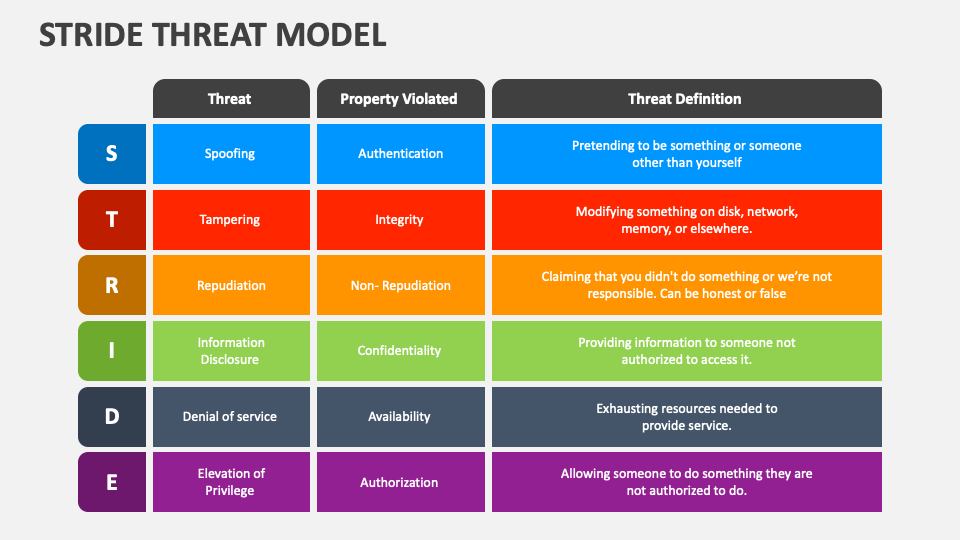
\includegraphics[width=0.7\textwidth]{img/stride-threat-model.png}
    \caption{Microsoft STRIDE Tehdit Modelleme Çerçevesi}
    \label{fig:stride-threat-model}
\end{figure}

STRIDE, genellikle geliştirme sürecinin tasarım aşamasında kullanılır ve sistem mimarisini analiz ederek potansiyel tehdit kategorilerini belirlemeye yardımcı olur.
\item \textbf{DREAD Metodolojisi:} DREAD, bir tehdidin ciddiyetini değerlendirmek için kullanılan nicel bir modeldir. Genellikle STRIDE ile birlikte kullanılır; STRIDE tehditleri belirlerken, DREAD bunların önceliklendirilmesine yardımcı olur. Her bir tehdit, beş kritere göre 1'den 10'a kadar bir puanla derecelendirilir:
\begin{itemize}
    \item \textbf{D}amage (Hasar): Saldırının potansiyel etkisi.
    \item \textbf{R}eproducibility (Tekrarlanabilirlik): Saldırının ne kadar kolay tekrarlanabildiği.
    \item \textbf{E}xploitability (İstismar Edilebilirlik): Zafiyetin ne kadar kolay istismar edilebildiği.
    \item \textbf{A}ffected Users (Etkilenen Kullanıcılar): Etkilenen kullanıcı sayısı.
    \item \textbf{D}iscoverability (Keşfedilebilirlik): Zafiyetin ne kadar kolay keşfedilebildiği.
\end{itemize}
Bu puanların ortalaması alınarak her bir tehdide bir önem derecesi atanır ve böylece düzeltme stratejileri önceliklendirilir.
\item \textbf{PASTA Metodolojisi (Process for Attack Simulation and Threat Analysis):} PASTA, yedi adımlı, saldırgan odaklı ve risk merkezli kapsamlı bir metodolojidir. Bu yaklaşım, tehditleri iş hedefleriyle ilişkilendirerek olgun güvenlik programlarına sahip büyük kuruluşlar için idealdir.
\end{itemize}
Tehdit modelleme çerçeveleri birbirini dışlayan yaklaşımlar değildir, aksine birbirini tamamlayan araçlar olarak kullanılabilir. STRIDE gibi bir model, potansiyel tehditlerin varlığını sistematik bir şekilde ortaya çıkarırken, DREAD bu tehditlerin ne kadar acil bir risk oluşturduğunu belirlemek için kullanılır. Bu sinerjik kullanım, sınırlı kaynakların en kritik güvenlik sorunlarına yönlendirilmesini sağlar. Ayrıca, PASTA'nın iş süreçlerini ve teknik tehditleri bir araya getirme yaklaşımı, tehdit modellemenin sadece teknik bir egzersiz değil, aynı zamanda stratejik bir iş faaliyeti olduğunu gösterir.
\textbf{Uygulamalı Senaryo:}
Bir e-ticaret uygulamasının kullanıcı profili güncelleme bileşenine yönelik tehdit modellemesi şu adımlarla gerçekleştirilebilir:
\begin{itemize}
\item Veri Akış Şeması (DFD) oluşturularak, kullanıcının profiline ilişkin verilerin nasıl hareket ettiği görselleştirilir.
\item STRIDE kullanılarak, her bir veri akışı ve işlem için olası tehditler listelenir. Örneğin, \texttt{HTTP POST} isteğiyle gönderilen kullanıcı verileri için "Kurcalama" tehdidi incelenir.
\item Tespit edilen her tehdit, DREAD kriterlerine göre puanlanarak en yüksek riske sahip olanlar önceliklendirilir. Bu sayede, güvenlik ekipleri en acil sorunlara odaklanabilir.
\end{itemize}
\subsection{Güvenli Kodlama Standartları ve En İyi Uygulamalar}
Güvenli kodlama, zafiyetlerin kaynak kod seviyesinde oluşmasını engellemek için benimsenen bir dizi disiplinli yaklaşımdır. Uygulamaların güvenliğini temelden sağlamlaştırmak için belirli prensiplere uyulması gerekir.
\begin{itemize}
\item \textbf{Varsayılan Olarak Reddetme (Default Deny):} Erişim kararlarının, özellikle yetkilendirme ve erişim kontrollerinde, varsayılan olarak reddetme üzerine inşa edilmesi esastır. Bu, yalnızca açıkça izin verilen koşullar altında erişime izin verilmesini sağlar.
\item \textbf{En Az Yetkilendirme (Principle of Least Privilege):} Her süreç veya kullanıcı, görevini tamamlamak için gerekli olan en az yetki setiyle çalışmalıdır. Bu yaklaşım, bir saldırganın sistemde yetki yükseltme yapma olasılığını azaltır.
\item \textbf{Girdi Doğrulama:} Tüm güvenilmeyen veri kaynaklarından (kullanıcı girdisi, API yanıtları, çevre değişkenleri) gelen verilerin titizlikle doğrulanması, zafiyetlerin büyük bir kısmını önleyebilir.
\item \textbf{Merkezi Güvenlik Kontrolleri:} Kimlik doğrulama, yetkilendirme ve girdi doğrulama gibi güvenlik işlevlerinin, tüm uygulama genelinde tek ve merkezi bir rutin aracılığıyla yapılması tavsiye edilir. Bu, güvenlik politikalarının tutarlı bir şekilde uygulanmasını sağlar.
\item \textbf{Savunmada Derinlik (Defense in Depth):} Bir savunma katmanının başarısız olması durumunda diğerlerinin koruma sağlaması için çoklu savunma stratejilerinin uygulanması gerekir. Bu prensip, güvenli programlama tekniklerinin güvenli çalışma zamanı ortamlarıyla birleştirilmesi gibi yöntemlerle desteklenebilir.
\end{itemize}
\subsection{Güvenlik Kod İncelemesi ve Statik Analiz (SAST) Entegrasyonu}
Statik Uygulama Güvenlik Testi (SAST), uygulamanın kaynak kodunu, bayt kodunu veya ikili kodunu çalıştırmadan analiz eden bir "beyaz kutu" test metodolojisidir. SAST, geliştirme yaşam döngüsünün en erken aşamalarında zafiyetleri (örn. SQL enjeksiyonları, arabellek taşmaları) tespit etme yeteneğine sahiptir.
Bir SAST aracı, kodu ayrıştırarak soyut bir sözdizimi ağacı (AST) oluşturur. Bu ağaç, kodun yapısını temsil eder ve aracın veri akışını izlemesine olanak tanır. Analiz, OWASP Top 10 ve CWE/SANS Top 25 gibi bilinen güvenlik standartlarına ve kurallarına göre yapılır. SAST, entegre geliştirme ortamlarına (IDE), versiyon kontrol sistemlerine ve CI/CD hatlarına entegre edilebilir. Bu sayede geliştiriciler, kodlarını kaydederken veya birleştirme isteği (pull request) oluştururken anında geri bildirim alabilirler. SAST'ın en büyük zorluklarından biri, yanlış pozitif (false positives) uyarı sayısının yüksek olabilmesidir. Ayrıca, SAST araçları kodda temsil edilmeyen, örneğin sunucu yapılandırması gibi sorunları tespit edemez.
\subsection{CI/CD Pipeline'larında Güvenlik Testi Entegrasyonu}
Modern yazılım geliştirme süreçlerinde, güvenlik testleri CI/CD (Sürekli Entegrasyon/Sürekli Dağıtım) boru hatlarına entegre edilerek otomatize edilir ve sürekli hale getirilir.
\begin{itemize}
\item \textbf{SAST:} SAST, CI/CD boru hattına \texttt{pre-commit} hook'ları veya build aşaması gibi en erken noktalarda entegre edilir. Örneğin, bir geliştirici kodunu göndermeden önce yerel bir tarama yaparak basit hataları hızlıca düzeltebilir.
\item \textbf{DAST (Dynamic Application Security Testing):} DAST, çalışan bir uygulama üzerinde "siyah kutu" testi yaparak gerçek bir saldırıyı simüle eder. Bu, SAST'ın gözden kaçırabileceği iş mantığı hataları, kimlik doğrulama bypass'ları veya yapılandırma zafiyetleri gibi çalışma zamanı (runtime) sorunlarını ortaya çıkarır. DAST taramaları genellikle boru hattının sonlarına doğru, staging veya QA ortamında otomatik olarak çalıştırılır.
\item \textbf{IAST (Interactive Application Security Testing):} IAST, SAST ve DAST'ın hibrit birleşimidir. Uygulama çalışırken içeriden analiz yaparak, zafiyetin tam olarak hangi kod satırında olduğunu saptar ve düşük yanlış pozitif oranıyla sonuç üretir. IAST, CI/CD hatlarına sorunsuz entegre olabilen tek dinamik test tekniği olarak öne çıkar ve geliştiricilere hızlı ve bağlamsal geri bildirim sağlar.
\end{itemize}
\begin{center}
\textbf{Tablo 4.1.5a: AST Metodolojileri - Temel Özellikler}

\begin{tabular}{|p{4cm}|p{6cm}|p{4cm}|}
\hline
\hline
\textbf{Metodoloji} & \textbf{Tanım} & \textbf{SDLC Konumu}  \\
\hline
\hline
\textbf{SAST} & Statik Uygulama Güvenlik Testi & Plan, Kod, Build  \\
\hline
\hline
\textbf{DAST} & Dinamik Uygulama Güvenlik Testi & Test, Dağıtım  \\
\hline
\hline
\textbf{IAST} & Etkileşimli Uygulama Güvenlik Testi & Test, QA  \\
\hline
\hline
\textbf{RASP} & Çalışma Zamanı Uygulama Koruması & Çalışma (Runtime)  \\
\hline
\hline
\textbf{SCA} & Yazılım Bileşen Analizi & Plan, Kod, Build  \\
\hline
\hline
\hline
\end{tabular}
\end{center}

\begin{center}
\textbf{Tablo 4.1.5b: AST Metodolojileri - Kapsamlar ve Özellikler}

\begin{tabular}{|p{4cm}|p{6cm}|p{4cm}|}
\hline
\hline
\textbf{Metodoloji} & \textbf{Kapsadığı Zafiyetler} & \textbf{Avantajları}  \\
\hline
\hline
\textbf{SAST} & SQLi, XSS, Buffer Overflow, Hardcoded Secrets & Erken geri bildirim, geniş kapsam  \\
\hline
\hline
\textbf{DAST} & SQLi, XSS, Kimlik Doğrulama, İş Mantığı & Gerçek saldırı simülasyonu  \\
\hline
\hline
\textbf{IAST} & SQLi, XSS, Veri Akışı Zafiyetleri & Düşük yanlış pozitif  \\
\hline
\hline
\textbf{RASP} & Bilinen ve sıfır-gün saldırıları & Gerçek zamanlı koruma  \\
\hline
\hline
\textbf{SCA} & Kütüphane zafiyetleri, lisans uyumu & Açık kaynak risk yönetimi  \\
\hline
\hline
\hline
\end{tabular}
\end{center}

\section{Web Uygulama Güvenliği ve OWASP Çerçevesi}

Web uygulama güvenliği, modern siber güvenlik stratejilerinin temel taşlarından biridir. Open Web Application Security Project (OWASP), web uygulamalarının güvenliğini artırmak için standartlar, araçlar ve en iyi uygulamalar sunan, kar amacı gütmeyen bir kuruluştur. OWASP'ın kaynak havuzu şunları içerir:

\begin{itemize}
\item \textbf{OWASP Top 10:} Web uygulamalarına yönelik en kritik on güvenlik riskini sıralayan ve düzenli olarak güncellenen bir liste. Bu liste, geliştiricilerin ve güvenlik profesyonellerinin en yaygın saldırı vektörlerine karşı savunma stratejileri oluşturmasına yardımcı olur.

\item \textbf{OWASP Testing Guide:} Kapsamlı bir web uygulama güvenlik testi rehberi. Test süreçlerini, metodolojileri ve araçları detaylıca açıklar.

\item \textbf{OWASP Code Review Guide:} Güvenli kod inceleme pratikleri için yol gösterici bir kaynak. Geliştiricilere ve güvenlik uzmanlarına yönelik rehberlik sağlar.

\item \textbf{OWASP Software Assurance Maturity Model (SAMM):} Organizasyonların yazılım güvenliği programlarını değerlendirmeleri ve geliştirmeleri için bir çerçeve sunar.

\item \textbf{OWASP Security Knowledge Framework (SKF):} Güvenli yazılım geliştirme için bir eğitim platformu ve kılavuz.

\item \textbf{OWASP DevSecOps Maturity Model:} DevSecOps olgunluğunu değerlendirmek ve geliştirmek için bir çerçeve sunar.

\item \textbf{OWASP Mobile Security Testing Guide (MASTG):} Mobil uygulama güvenlik testi için kapsamlı bir rehber.

\item \textbf{OWASP Web Security Testing Guide (WSTG):} Web uygulaması güvenlik testi için metodolojiler ve örnekler sunar.

\item \textbf{OWASP API Security Top 10:} API güvenliğindeki en kritik riskleri tanımlar.
\end{itemize}

OWASP, düzenli olarak güncellenen, gönüllü topluluğun katkılarıyla gelişen ve açık kaynak prensiplerini benimseyen bir projedir. Kuruluşların güvenlik olgunluğunu artırmak için birçok farklı araç ve çerçeve sunar.

\subsection{OWASP Top 10 Güvenlik Açıkları ve Azaltma Stratejileri}

OWASP Top 10, web uygulamaları için en kritik on riskin konsensüs listesidir. Bu liste, güvenlik uzmanlarının ve geliştiricilerin en önemli zafiyetlere odaklanmasına yardımcı olur.

\begin{figure}[H]
    \centering
    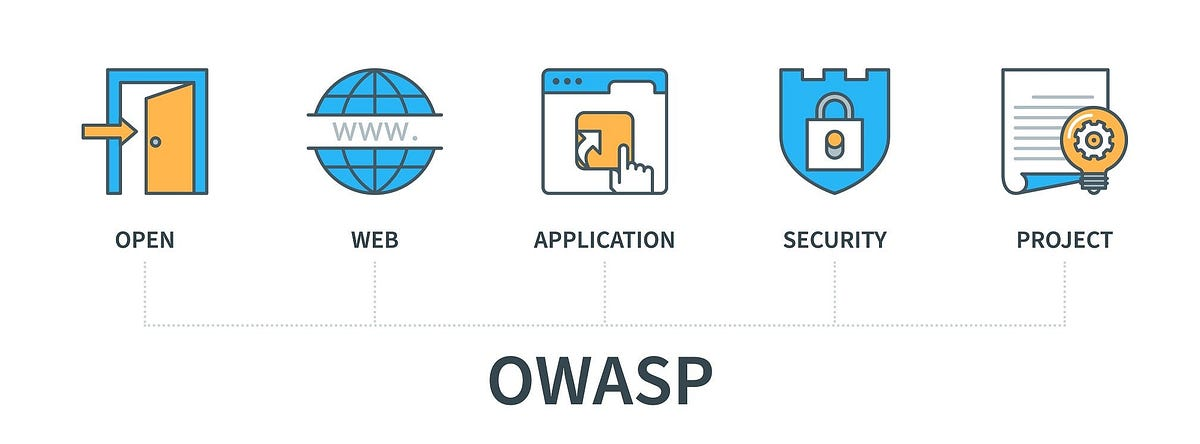
\includegraphics[width=0.6\textwidth]{img/owasp-standsfor.png}
    \caption{OWASP (Open Web Application Security Project) Logosu ve Açılımı}
    \label{fig:owasp-logo}
\end{figure}



\begin{itemize}
\item \textbf{A01:2021 Bozuk Erişim Kontrolü (Broken Access Control):} 2021 listesinde birinci sıraya yükselen bu zafiyet, bir saldırganın yetkisi olmayan kullanıcı hesaplarına veya işlevlere erişimini sağlar. Örneğin, bir URL'deki kullanıcı kimliğini temsil eden birincil anahtarın değiştirilmesiyle, bir saldırgan başka bir kullanıcının hesabını görüntüleyebilir veya düzenleyebilir. Bu tür zafiyetlerin giderilmesi için IAST araçları kullanılabilir ve mimari tasarımda güven sınırları oluşturulması gerekebilir.
\item \textbf{A02:2021 Kriptografik Başarısızlıklar (Cryptographic Failures):} Daha önce "Hassas Veri Açığa Çıkması" olarak bilinen bu risk, parolalar, kimlik numaraları gibi hassas verilerin depolanması veya iletilmesi sırasında yetersiz şekilde korunmasıyla ilgilidir. Zayıf şifreleme algoritmaları veya sabit kodlanmış kriptografik anahtarlar gibi kök nedenlere odaklanır. SAST ve SCA araçları, zayıf şifreleme gücü ve riskli algoritmaları tarayarak bu riskleri azaltmaya yardımcı olurken, IAST sürekli izleme sağlar.
\item \textbf{A03:2021 Enjeksiyon (Injection):} Listede üçüncü sırada yer alan enjeksiyon, güvensiz verilerin komut veya sorgu olarak yorumlanması sonucu meydana gelir. En yaygın türleri SQL enjeksiyonu ve artık bu kategoriye dahil edilen XSS'tir.
\end{itemize}

\subsection{Girdi Doğrulama, Çıktı Kodlama ve Parametreli Sorgular}

Bu üç teknik, enjeksiyon saldırılarına karşı birincil savunma mekanizmalarıdır.

\begin{itemize}
\item \textbf{Girdi Doğrulama (Input Validation):} Güvenilmeyen kaynaklardan gelen verinin, beklenen format, tip ve uzunluk gibi önceden tanımlanmış kriterlere uyduğunu doğrular. En güvenli yaklaşım, yalnızca kabul edilebilir karakter veya formatları tanımlayan bir "beyaz liste" (allowlist) kullanmaktır, "kara liste" (denylist) ise eksik olabilir ve yeni saldırı vektörlerine karşı savunmasız kalabilir. Sunucu tarafında uygulanması zorunludur, çünkü istemci tarafı doğrulama kolayca atlatılabilir.
\item \textbf{Çıktı Kodlama (Output Encoding):} Bir uygulamanın, kullanıcıdan gelen veriyi tarayıcı veya başka bir yorumlayıcıya göndermeden önce potansiyel olarak zararlı karakterleri güvenli bir formata dönüştürmesidir. Bu, karakterlerin kod olarak değil, salt metin olarak görüntülenmesini sağlar ve XSS saldırılarını önlemede kritik bir rol oynar.
\item \textbf{Parametreli Sorgular (Parameterized Queries):} SQL enjeksiyonuna karşı en etkili savunma yöntemidir. Bu teknik, SQL kod yapısını kullanıcıdan gelen veriden ayırır, böylece girdi yalnızca bir veri değeri olarak işlenir ve kötü amaçlı komutların veritabanı tarafından yürütülmesini engeller.
\end{itemize}

\subsection{Kimlik Doğrulama ve Oturum Yönetimi Güvenliği}

Kimlik doğrulama, kullanıcıyı doğrulamayı, oturum yönetimi ise bu doğrulama sonrası kullanıcı oturumunu güvenli bir şekilde sürdürmeyi amaçlar.

\begin{itemize}
\item \textbf{Oturum Güvenlik Açıkları:} İlgili riskler arasında bir saldırganın geçerli bir oturum belirtecini ele geçirdiği \textbf{Oturum Korsanlığı (Session Hijacking)} ve bir kullanıcıyı önceden belirlenmiş bir oturum kimliği kullanmaya zorladığı \textbf{Oturum Sabitleme (Session Fixation)} yer alır.
\item \textbf{En İyi Uygulamalar:} Oturum kimlikleri, yeterli rastgeleliğe (en az 64 bit entropi) sahip bir CSPRNG (Kriptografik Olarak Güvenli Sözde Rastgele Sayı Üreteci) ile oluşturulmalıdır. Oturum çerezlerinin \texttt{HttpOnly} bayrağı ile korunması, JavaScript'in çereze erişimini engeller ve XSS saldırılarına karşı bir savunma katmanı sağlar. Oturumların, hem kullanıcı çıkış yaptığında hem de bir süre işlem yapılmadığında güvenli bir şekilde sonlandırılması gereklidir.
\end{itemize}

\subsection{Cross-Site Scripting (XSS) ve Cross-Site Request Forgery (CSRF)}

XSS ve CSRF, web uygulamalarının kullanıcılarına duyduğu "güven"i istismar eden iki farklı ancak birbiriyle ilişkili saldırı türüdür.

\begin{itemize}
\item \textbf{XSS (Siteler Arası Komut Dosyası Çalıştırma):} Saldırgan, bir web uygulamasına kötü amaçlı bir komut dosyası enjekte ederek bu betiğin diğer kullanıcıların tarayıcılarında çalışmasını sağlar. Bu, uygulamanın kullanıcı girdisini yeterince filtrelememesinden kaynaklanır. Azaltım stratejileri, girdi doğrulaması, çıktı kodlaması ve DOMPurify gibi kütüphanelerle HTML sanitizasyonunu içerir.
\item \textbf{CSRF (Siteler Arası İstek Sahteciliği):} Bu saldırıda, bir saldırgan bir kullanıcıyı, rızası olmadan bir eylem gerçekleştirmesi için sahte bir istek göndermesi için kandırır. Saldırganın hedefi, uygulamanın kullanıcının oturum kimliğine ve dolayısıyla isteğin meşruiyetine olan güvenini istismar etmektir. En yaygın savunma, her istek için benzersiz ve öngörülemez bir \textbf{CSRF belirteci} (token) kullanmaktır.
\end{itemize}

XSS ve CSRF, farklı güvenlik zafiyetleri olmasına rağmen, birbirlerinin savunmasını etkileyebilir. Bir saldırgan XSS ile başarılı olursa, \texttt{HttpOnly} bayrağı olmayan oturum çerezlerini ele geçirerek oturum korsanlığına zemin hazırlayabilir. Ancak, CSRF belirteçleri gibi bir kontrol, XSS saldırılarına karşı ikincil bir savunma katmanı sağlayabilir. Bir saldırgan XSS ile kötü amaçlı bir betik enjekte etse bile, bu betik, istek için geçerli olan benzersiz CSRF belirtecine erişemez ve bu da saldırının engellenmesine yardımcı olur. Bu durum, güvenlik kontrollerinin birbirini desteklemesi gerektiğini vurgulayan "savunmada derinlik" prensibinin bir yansımasıdır.

\subsection{İçerik Güvenlik Politikası (CSP) ve Güvenlik Başlıkları}

İçerik Güvenlik Politikası (CSP), bir web uygulamasının güvenlik modeline ikinci bir savunma katmanı ekleyen bir güvenlik başlığıdır. Sunucu tarafından gönderilen bu HTTP başlığı, tarayıcıya, betikler, stiller, resimler gibi hangi kaynaklardan içerik yükleyebileceğini bildirir.

CSP, XSS saldırılarına karşı birden fazla şekilde koruma sağlar:

\begin{itemize}
\item \textbf{Satır İçi Betik Kısıtlaması:} \texttt{inline} (satır içi) \textless script\textgreater{} etiketlerinin çalışmasını engeller.
\item \textbf{Uzak Kaynak Kısıtlaması:} Rastgele sunuculardan betik yüklenmesini engeller.
\item \textbf{Güvenli Olmayan Fonksiyonların Engellenmesi:} \texttt{eval()} gibi güvensiz JavaScript fonksiyonlarının yürütülmesini kısıtlar.
\item \textbf{Form Kısıtlaması:} HTML formlarının yalnızca belirlenen güvenilir hedeflere veri göndermesini sağlar, bu da kimlik avı formlarının enjekte edilmesini önler.
\end{itemize}

CSP, "yalnızca raporlama" moduyla test edilebilir veya doğrudan etkinleştirilerek zorunlu hale getirilebilir. Güvenlik başlıklarının doğru bir şekilde yapılandırılması, uygulamanın genel güvenlik duruşunu önemli ölçüde artırır.

\section{API Güvenliği ve Microservices Mimarisi}

API'ler (Application Programming Interfaces), modern yazılım mimarilerinin temel bir bileşenidir ve farklı uygulamaların birbirleriyle iletişim kurmasını sağlar. Mikroservis mimarileri, büyük ve monolitik uygulamaları daha küçük, bağımsız hizmetlere ayırarak geliştirme ve dağıtım süreçlerini kolaylaştırır. Ancak, bu mimari aynı zamanda yeni güvenlik zorlukları da ortaya çıkarır. Her bir mikroservis ve API, potansiyel bir saldırı yüzeyi oluşturur ve bu nedenle güvenli bir şekilde tasarlanmalı ve yönetilmelidir.

\subsection{RESTful API Güvenliği En İyi Uygulamaları}

RESTful API'ler, web uygulamalarıyla aynı seviyede veya daha fazla güvenlik riskine sahiptir. Bu nedenle, tasarım aşamasından itibaren katı güvenlik prensiplerinin uygulanması gereklidir.

\begin{itemize}
\item \textbf{Her Zaman TLS Şifrelemesi Kullanın:} Tüm API iletişimleri, uçtan uca veri şifrelemesi sağlamak için TLS (Transport Layer Security) ile korunmalıdır. Bu, ağ trafiği içindeki parolalar, API anahtarları veya tokenlar gibi hassas bilgilerin gizliliğini sağlar.
\item \textbf{Güçlü Kimlik Doğrulama ve Yetkilendirme Modeli:} API anahtarları ve güvenlik tokenları gibi yöntemlerle ölçeklenebilir bir modelin uygulanması esastır. Bu süreç, özellikle OAuth 2.0 ve OpenID Connect gibi standartlarla entegre bir şekilde yürütüldüğünde, daha güvenli ve yönetilebilir hale gelir.
\item \textbf{Hassas Bilgileri URL'de Tutmayın:} Bir RESTful API tasarım hatası, kullanıcı kimlik bilgileri veya tokenlar gibi hassas verilerin URL'lere eklenmesidir. Bu, TLS kullanılsa dahi, verilerin sunucu günlüklerinde veya ağ cihazlarında kolayca keşfedilmesine yol açabilir.
\item \textbf{İstek ve Yanıtları Dar Tanımlayın:} Saldırganların API'leri kötü niyetli veya amaç dışı kullanmaya çalışacağını varsaymak önemlidir. Bu nedenle, gelen parametrelerin formatı, uzunluğu ve tipi gibi nitelikleri titizlikle doğrulanmalı, API yanıtları ise yalnızca açıkça izin verilen içerikle sınırlı tutulmalıdır.
\item \textbf{Sürekli API Keşfi:} "Gölge" (shadow) API'leri (standart süreçler dışında geliştirilenler) ve "zombi" (zombie) API'leri (unutulmuş eski altyapılardaki riskler) gibi varlıkları belirlemek için sürekli bir envanter yönetimi ve keşif yeteneği uygulanmalıdır.
\end{itemize}

\subsection{OAuth 2.0, OpenID Connect ve JWT Token Güvenliği}

Bu üç teknoloji, API güvenliği için modern kimlik doğrulama ve yetkilendirme standartlarını oluşturur.

\begin{itemize}
\item \textbf{OAuth 2.0:} Bir yetkilendirme çerçevesidir. Kullanıcının parolalarını paylaşmadan, bir uygulamaya kendi adına belirli kaynaklara erişim izni vermesini sağlar.
\item \textbf{OpenID Connect (OIDC):} OAuth 2.0 üzerine inşa edilmiş, kimlik doğrulama katmanı ekleyen bir protokoldür. Bir kullanıcının kimliğini doğrulamak ve temel profil bilgilerini almak için kullanılır.
\item \textbf{JWT (JSON Web Token):} JSON tabanlı, sıkıştırılmış ve güvenli bir belirteç formatıdır. OIDC ve OAuth 2.0'da kimlik ve erişim belirteçlerini iletmek için kullanılır.
\item \textbf{JWT Güvenliği:}
\begin{itemize}
\item \textbf{Doğrulama:} Gelen her JWT, her istekte imzası, süresi (\texttt{exp}) ve yayıncısı (\texttt{iss}) gibi iddialarının (\texttt{claims}) doğrulanması zorunludur. Bu, tokenın sahte veya kurcalanmış olmadığını garanti eder.
\item \textbf{Güvenli Saklama:} JWT'ler, Çapraz Site Komut Dosyası Çalıştırma (XSS) saldırılarına karşı \texttt{HttpOnly} ve \texttt{Secure} bayraklarına sahip çerezlerde saklanmalıdır. \texttt{localStorage} veya \texttt{sessionStorage} gibi tarayıcı depolama alanları, JavaScript tarafından erişilebilir oldukları için XSS'e karşı savunmasızdır.
\item \textbf{Kısa Yaşam Süresi:} JWT'lerin kısa ömürlü olması, token çalınması durumunda saldırganın etki süresini sınırlar. Bu tokenlar, daha uzun ömürlü ancak daha güvenli bir şekilde saklanan yenileme belirteçleriyle (refresh tokens) birlikte kullanılmalıdır.
\end{itemize}
\end{itemize}

\subsection{API Gateway Güvenlik Özellikleri ve Hız Sınırlandırma (Rate Limiting)}

Mikroservis mimarisinde, bir API Gateway, hizmetler için tek bir giriş noktası görevi görür. Bu merkezi konum, kimlik doğrulama, yetkilendirme, izleme ve özellikle hız sınırlama gibi güvenlik kontrollerinin tutarlı bir şekilde uygulanmasını sağlar.

\begin{itemize}
\item \textbf{Hız Sınırlandırma (Rate Limiting):} Bir istemcinin belirli bir zaman diliminde API'ye gönderebileceği istek sayısını kontrol eden bir mekanizmadır. Bu, hizmet reddi (DoS) ve kaba kuvvet saldırılarını önlemenin yanı sıra, sistemin aşırı yüklenmesini engeller ve adil kaynak dağılımını sağlar.
\item \textbf{Algoritmalar:} En yaygın kullanılan hız sınırlama algoritmaları arasında \textbf{Sabit Pencere Sayacı (Fixed Window Counter)}, \textbf{Kaydırılan Günlük (Sliding Log)} ve ani trafik artışlarını yönetmek için ideal olan \textbf{Token Kovası (Token Bucket)} yer alır.
\end{itemize}

\subsection{GraphQL Güvenlik Hususları}

GraphQL, esnekliği sayesinde geliştiriciler arasında popülerlik kazanmıştır, ancak bu esneklik kendine özgü güvenlik tehditlerini de beraberinde getirir.

\begin{itemize}
\item \textbf{DoS Saldırıları:} GraphQL'in iç içe geçmiş sorgulara (nested queries) izin vermesi, bir saldırganın tek bir istekte çok fazla kaynak talep ederek hizmet reddi (DoS) saldırısı gerçekleştirmesine olanak tanır.
\item \textbf{Azaltım:} Sorgu derinliği ve maliyet analizi sınırlamaları uygulanmalıdır. Bu kontroller, bir sorgunun karmaşıklığına göre sunucunun tüketebileceği maksimum kaynak miktarını sınırlar.
\item \textbf{Yetkilendirme:} GraphQL API'leri, talep edilen veriler üzerinde yetkilendirme kontrollerini titizlikle uygulamalıdır. Yetkilendirme kontrollerinin hem düğümler (\texttt{nodes}) hem de kenarlar (\texttt{edges}) üzerinde uygulanması, Broken Object Level Authorization (BOLA) gibi zafiyetleri önler.
\item \textbf{Güvenli Yapılandırma:} Üretim ortamlarında, API'nin yapısını keşfetmeyi sağlayan \textbf{Introspection} sorguları devre dışı bırakılmalı veya yalnızca yetkili kullanıcılara açık olmalıdır. Ayrıca, hata mesajlarında gereksiz iç sistem bilgilerinin (örn. yığın izleri) açığa çıkması engellenmelidir.
\end{itemize}

\subsection{Microservices İletişim Güvenliği (mTLS, Service Mesh)}

Mikroservisler arası iletişim, genellikle bir ağ üzerinden gerçekleştiği için ortadaki adam (MITM) ve kimliğe bürünme saldırılarına açıktır.

\begin{itemize}
\item \textbf{mTLS (Mutual TLS):} Geleneksel TLS'nin aksine, mTLS'de hem istemci hem de sunucu, iletişim başlamadan önce birbirlerinin kimliklerini doğrular. Bu, sıfır güven (zero-trust) mimarilerinin temelini oluşturan, karşılıklı kimlik doğrulama ve şifreleme sağlar. Uygulama, OpenSSL gibi araçlarla sertifika ve anahtar çiftleri oluşturularak adım adım uygulanabilir.
\item \textbf{Service Mesh:} Mikroservisler arası iletişimin güvenliğini, izlenebilirliğini ve yönetimini sağlayan bir altyapı katmanıdır. Service Mesh, mTLS'i hizmetler için otomatik olarak yönetir, bu da her bir hizmetin kendi güvenlik mantığını uygulamasına gerek kalmamasını sağlar.
\end{itemize}

Service Mesh, mTLS'in tek başına yeterli olmadığı yetkilendirme sorununu da ele alır. mTLS bir hizmetin kimliğini doğrular, ancak o hizmetin belirli bir eylemi yapmaya yetkili olup olmadığını garantilemez. Service Mesh, yetkilendirme kurallarını merkezi olarak tanımlama ve uygulama yeteneği sunarak, sıfır güven mimarisinin "asla güvenme, her zaman doğrula" prensibini en iyi şekilde uygulamayı mümkün kılar. Bu, güvenlik politikasını ağ katmanından daha granüler olan iş yükü (pod) seviyesine taşıyarak daha sağlam bir koruma sağlar.

\section{Uygulama Güvenlik Testi (AST) Metodolojileri}

Uygulama Güvenlik Testi (AST), yazılım geliştirme yaşam döngüsü boyunca güvenlik açıklarını tespit etmek ve düzeltmek için kullanılan bir dizi metodolojiyi ifade eder. AST, statik, dinamik ve interaktif test yaklaşımlarını içerir.

\subsection{Statik Uygulama Güvenlik Testi (SAST) Araçları}

SAST, kaynak kodun, bayt kodun veya ikili kodun çalıştırılmadan analizini yapar. Bu "beyaz kutu" test metodolojisi, SQL enjeksiyonları, arabellek taşmaları ve XSS gibi güvenlik açıklarını, yazılım geliştirme yaşam döngüsünün çok erken aşamalarında, hatta kod derlenmeden önce bile tespit edebilir. SAST araçları, kodun tamamını tarayarak potansiyel güvenlik zafiyetlerini belirler. Bu araçlar, geliştirme boru hatlarına, IDE'lere ve versiyon kontrol sistemlerine entegre edilebilir.

\subsection{Dinamik Uygulama Güvenlik Testi (DAST) Otomasyonu}

DAST, bir uygulamayı çalıştığı sırada test ederek, gerçek dünya saldırılarını simüle eden "siyah kutu" bir yaklaşımdır. Bu yöntem, kaynak koduna erişim olmaksızın, uygulamanın dış arayüzleri aracılığıyla zafiyetleri tespit etmeye odaklanır. DAST, SAST'ın gözden kaçırabileceği kimlik doğrulama bypass'ları, zayıf parolalar veya iş mantığı hataları gibi çalışma zamanı sorunlarını ortaya çıkarır. CI/CD boru hatlarına entegre edilerek, kod derlemesi veya her kod gönderiminde otomatik taramalar gerçekleştirilebilir.

\subsection{Etkileşimli Uygulama Güvenlik Testi (IAST) Faydaları}

IAST, bir uygulamanın içinde çalışarak SAST ve DAST'ın güçlü yönlerini birleştiren hibrit bir metodolojidir. IAST, uygulamanın çalışma zamanı davranışını izleyerek zafiyetin tam olarak hangi kod satırında olduğunu saptar ve bu sayede düzeltme sürecini geliştiriciler için çok daha hızlı hale getirir. DAST'ın aksine, IAST düşük yanlış pozitif oranıyla sonuç üretir ve CI/CD hatlarına sorunsuz bir şekilde entegre olabilen tek dinamik test tekniğidir. Bu sayede, güvenlik kontrolleri geliştiricinin iş akışını bozmadan sürekli olarak uygulanabilir.

\subsection{Çalışma Zamanı Uygulama Kendi Kendini Koruma (RASP) Uygulaması}

RASP, uygulamanın içine yerleştirilen ve canlı ortamda saldırıları gerçek zamanlı olarak algılayıp engelleyen bir güvenlik teknolojisidir. Bir RASP aracı, bir ağ güvenlik duvarı (WAF) gibi ağ tabanlı çözümlerden farklı olarak, uygulamanın davranışını ve içinde gerçekleşen olayları analiz eder. Bu sayede, saldırgan çevre savunmasını aştıktan sonra bile uygulamayı koruyabilir ve SQL enjeksiyonu veya XSS gibi saldırıları, uygulamaya ulaşmadan önce engelleyebilir. RASP, uygulamanın kodunda herhangi bir değişiklik yapılmasını gerektirmez, bu da mevcut uygulamaların kolayca korunmasını sağlar.

\subsection{Yazılım Bileşen Analizi (SCA) ve Açık Kaynak Güvenliği}

Yazılım Bileşen Analizi (SCA), uygulamalarda kullanılan üçüncü taraf ve açık kaynak bileşenleri tarayarak bilinen güvenlik zafiyetlerini ve lisans uyumluluğu sorunlarını bulur. Açık kaynak bileşenleri, bilinen zafiyetler içerebileceğinden, bu zafiyetlerin üretime dağıtılmadan önce belirlenmesi ve yönetilmesi hayati önem taşır.

SCA'nın en iyi uygulamalarından biri, her derleme (build) için bir Yazılım Malzeme Listesi (SBOM) oluşturmaktır. SBOM, projedeki tüm yazılım bileşenlerinin detaylı bir envanterini sunar ve sıfır gün (zero-day) zafiyetleri gibi durumlarda etkilenen bileşenlerin hızlıca tespit edilmesini sağlar. SCA'yı CI/CD boru hattına entegre etmek, politikalara aykırı veya risk içeren birleştirme isteklerinin (pull requests) ana kod tabanına birleşmesini otomatik olarak engellemeye yardımcı olur. Bu, geliştirme sürecini yavaşlatmadan güvenliği sürekli kılar.

\section{DevSecOps Entegrasyonu ve CI/CD Pipeline Güvenliği}

DevSecOps, geliştirme (Development), güvenlik (Security) ve operasyon (Operations) ekiplerini bir araya getirerek, güvenlik kontrollerini yazılım geliştirme yaşam döngüsünün her aşamasına entegre eden bir yaklaşımdır. Bu model, güvenliği bir "sonradan eklenen" bir özellik olarak değil, sürecin ayrılmaz bir parçası olarak ele alır. CI/CD (Continuous Integration/Continuous Deployment) pipeline'ları, yazılımın hızlı ve otomatik bir şekilde oluşturulmasını, test edilmesini ve dağıtılmasını sağlar. Bu pipeline'lara güvenlik kontrollerinin entegre edilmesi, güvenlik açıklarının erken tespit edilmesine ve düzeltilmesine olanak tanır.

\subsection{Modern DevSecOps Toolchain ve Cloud-Native Security}

Güvenlik otomasyonu, modern yazılım geliştirmede ölçeklenebilirlik, esneklik ve uyumluluk sağlamanın temelidir. Bu, güvenlik tarama araçlarının (SAST, SCA) geliştirici iş akışına ve \texttt{pre-commit} hook'larına entegre edilmesiyle başlar. Otomatik güvenlik araçları, her kod gönderiminde veya birleştirme isteğinde çalıştırılarak geliştiricilere anında geri bildirim sağlar.

\textbf{Modern DevSecOps Tool Ecosystem:}
\begin{itemize}
    \item \textbf{Source Code Security:} GitHub Advanced Security, GitLab Ultimate Security features
    \item \textbf{CI/CD Integration:} Jenkins Security plugins, Azure DevOps Security extensions
    \item \textbf{Infrastructure Security:} Terraform Cloud Policy sets, AWS Config Rules
    \item \textbf{Runtime Protection:} Falco runtime security, Twistlock/Prisma Cloud
    \item \textbf{Supply Chain Security:} Sigstore (Cosign/Rekor), SLSA framework compliance
\end{itemize}

\textbf{Cloud-Native Security Integration Patterns:}
\begin{lstlisting}[breaklines=true,basicstyle=\ttfamily\footnotesize]
// GitOps Security Pipeline Orchestrator
public class CloudNativeSecurityPipeline {
    private final ContainerSecurityScanner containerScanner;
    private final InfrastructureValidator infraValidator;
    private final PolicyEngine policyEngine;
    private final SBOMGenerator sbomGenerator;
    
    public PipelineResult executeSecurityGates(BuildContext context) {
        // 1. Pre-commit Security Hooks
        PreCommitResults preCommit = executePreCommitHooks(context);
        if (!preCommit.isSecurityCompliant()) {
            return PipelineResult.failed("Pre-commit security checks failed");
        }
        
        // 2. Source Code Security Analysis
        SCAResults scaResults = containerScanner.scanSourceCode(context.getRepository());
        SASTResults sastResults = performStaticAnalysis(context);
        
        // 3. Infrastructure as Code Security Validation
        IaCSecurityResults iacResults = infraValidator.validateInfrastructure(
            context.getTerraformFiles(),
            context.getKubernetesManifests()
        );
        
        // 4. Software Bill of Materials (SBOM) Generation
        SBOM sbom = sbomGenerator.generateSBOM(context);
        validateSBOMCompliance(sbom);
        
        // 5. Container Image Security Scanning
        ContainerScanResults containerResults = containerScanner.scanImages(
            context.getContainerImages()
        );
        
        // 6. Policy Compliance Validation
        PolicyValidationResults policyResults = policyEngine.validateCompliance(
            scaResults, sastResults, iacResults, containerResults
        );
        
        // 7. Security Gate Decision
        SecurityGateDecision decision = evaluateSecurityGates(
            preCommit, scaResults, sastResults, iacResults, containerResults, policyResults
        );
        
        return PipelineResult.builder()
            .securityGateDecision(decision)
            .sbom(sbom)
            .securityMetrics(generateSecurityMetrics(scaResults, sastResults))
            .remediationActions(generateRemediationPlan(decision))
            .build();
    }
    
    private SecurityGateDecision evaluateSecurityGates(
        PreCommitResults preCommit,
        SCAResults sca,
        SASTResults sast,
        IaCSecurityResults iac,
        ContainerScanResults container,
        PolicyValidationResults policy) {
        
        // Define security thresholds
        int criticalVulnerabilityThreshold = 0;
        int highVulnerabilityThreshold = 5;
        double securityScoreThreshold = 8.0;
        
        SecurityScore overallScore = calculateOverallSecurityScore(
            sca, sast, iac, container
        );
        
        if (overallScore.getCriticalCount() > criticalVulnerabilityThreshold) {
            return SecurityGateDecision.BLOCK_DEPLOYMENT;
        }
        
        if (overallScore.getHighCount() > highVulnerabilityThreshold) {
            return SecurityGateDecision.REQUIRE_APPROVAL;
        }
        
        if (overallScore.getOverallScore() < securityScoreThreshold) {
            return SecurityGateDecision.CONDITIONAL_APPROVAL;
        }
        
        return SecurityGateDecision.APPROVE_DEPLOYMENT;
    }
}
\end{lstlisting}

Bu araçların doğru bir şekilde orkestrasyonu, tehditlerin otomatik olarak algılanmasını ve yanıt verilmesini sağlar. Güvenlik olayları, izleme araçları tarafından tespit edildiğinde, otomatik düzeltme iş akışlarını tetikleyebilir.

\subsection{Supply Chain Security ve SLSA Framework}

Modern yazılım geliştirmede supply chain security kritik önem kazanmıştır. SolarWinds, Codecov ve Log4Shell gibi olaylar, yazılım tedarik zinciri saldırılarının ne kadar yaygın ve etkili olabileceğini göstermiştir.

\textbf{Supply Chain Attack Vectors:}
\begin{itemize}
    \item \textbf{Dependency Confusion:} Public repositories'de malicious packages ile legitimate internal packages'ın karıştırılması
    \item \textbf{Typosquatting:} Popüler package names'e benzer isimlerle malicious packages publish etme
    \item \textbf{Build System Compromise:} CI/CD pipeline'larına unauthorized code injection
    \item \textbf{Source Code Repository Compromise:} Legitimate repositories'e malicious commits
\end{itemize}

\textbf{SLSA (Supply-chain Levels for Software Artifacts) Framework Implementation:}
\begin{lstlisting}[breaklines=true,basicstyle=\ttfamily\footnotesize,language=Java]
// SLSA Compliance Engine
public class SLSAComplianceValidator {
    
    public SLSALevel validateSLSACompliance(BuildArtifact artifact) {
        // SLSA Level 1: Documentation of build process
        boolean hasSourceTracking = validateSourceTracking(artifact);
        boolean hasBuildService = validateBuildService(artifact);
        
        if (!hasSourceTracking || !hasBuildService) {
            return SLSALevel.NON_COMPLIANT;
        }
        
        // SLSA Level 2: Tamper resistance of build service
        boolean hasHostedBuildService = validateHostedBuildService(artifact);
        boolean hasSourceIntegrity = validateSourceIntegrity(artifact);
        
        if (!hasHostedBuildService || !hasSourceIntegrity) {
            return SLSALevel.LEVEL_1;
        }
        
        // SLSA Level 3: Extra resistance to specific threats
        boolean hasHardenedBuilds = validateHardenedBuilds(artifact);
        boolean hasProvenanceNonForgeable = validateProvenanceAuthenticity(artifact);
        
        if (!hasHardenedBuilds || !hasProvenanceNonForgeable) {
            return SLSALevel.LEVEL_2;
        }
        
        // SLSA Level 4: Highest levels of confidence and trust
        boolean hasTwoPersonReview = validateTwoPersonReview(artifact);
        boolean hasHermetic = validateHermeticBuilds(artifact);
        
        if (hasTwoPersonReview && hasHermetic) {
            return SLSALevel.LEVEL_4;
        }
        
        return SLSALevel.LEVEL_3;
    }
    
    private boolean validateSourceIntegrity(BuildArtifact artifact) {
        // Verify cryptographic signatures on source commits
        return artifact.getSourceCommits().stream()
            .allMatch(commit -> verifyCommitSignature(commit));
    }
    
    private boolean validateProvenanceAuthenticity(BuildArtifact artifact) {
        // Verify build provenance using Sigstore/Rekor
        return sigstoreClient.verifyProvenance(
            artifact.getProvenanceStatement(),
            artifact.getSignature()
        );
    }
}
\end{lstlisting}

\textbf{Software Bill of Materials (SBOM) Advanced Implementation:}
\begin{itemize}
    \item \textbf{SPDX Format Support:} Industry-standard SBOM format compliance
    \item \textbf{CycloneDX Integration:} Vulnerability ve license tracking
    \item \textbf{Dependency Graph Analysis:} Transitive dependency risk assessment
    \item \textbf{Continuous SBOM Updates:} Runtime dependency monitoring ve alerting
\end{itemize}

\subsection{Konteyner Güvenliği Taraması ve İmge Zafiyet Yönetimi}

Konteyner imajları, zafiyet içeren üçüncü taraf kütüphaneleri ve paketleri içerebilir. Bu zafiyetlerin üretime dağıtılmadan önce belirlenmesi zorunludur. Konteyner güvenliği taraması, bir konteyner imajındaki bilinen zafiyetleri, hatalı yapılandırmaları ve diğer güvenlik sorunlarını tanımlayan bir süreçtir.

Otomatik konteyner taraması, CI/CD boru hattına entegre edilerek, her derleme veya dağıtım aşamasında imajların sürekli olarak taranmasını sağlar. Bu taramaların sonuçları, zafiyetin açıklaması, ciddiyeti ve düzeltme adımları gibi ayrıntılı bilgiler içerir. En iyi uygulama, yüksek riskli zafiyetler içeren imajların dağıtımını otomasyonla engellemektir. Bu, dağıtım kapıları (security gates) aracılığıyla uygulanabilir.

\subsection{Kod Olarak Altyapı (IaC) Güvenlik Taraması}

Kod Olarak Altyapı (IaC), (örn. Terraform, CloudFormation), altyapıyı kod olarak yönetmeyi sağlar. Bu kodlar, açık ağ portları veya sabit kodlanmış kimlik bilgileri gibi hatalı yapılandırmalar içerebilir. IaC güvenlik taraması, bu tür hataları altyapı dağıtılmadan önce tespit eden bir güvenlik kontrolüdür. Bu süreç, IaC dosyalarını analiz ederek önceden tanımlanmış güvenlik politikaları ve kurallarına aykırı olan riskli ayarları işaretler. Böylece, altyapı dağıtımı sırasında oluşabilecek güvenlik zafiyetleri proaktif olarak engellenir.

\subsection{DevOps'ta Güvenlik Kapıları ve Kalite Kontrolü}

Güvenlik kapısı (Security Gate), bir yazılımın bir sonraki aşamaya geçmesi için karşılaması gereken bir dizi güvenlik gereksinimidir. Bu kapılar, bir derlemenin (build) devam etmesi için belirli bir eşiğin altında güvenlik sorunu barındırması gibi koşulları belirleyebilir.

Otomatik güvenlik taramaları bir "geçti/kaldı" kriteri olarak yapılandırılarak, belirlenen eşiğin altındaki güvenlik sorunları çözülmeden boru hattının ilerlemesi engellenir. Bu, teknik borcun birikmesini önler ve güvenliğin sonradan eklenen bir düşünce değil, sürecin doğal bir parçası olmasını sağlar. Güvenlik kapıları, ürün kalitesi ve güvenliğin ayrılmaz bir şekilde bağlantılı olduğunu vurgular.

\subsection{Sola Kaydırma (Shift-Left) Güvenlik Kültürü ve Geliştirici Eğitimi}

DevSecOps'un başarısı, güvenlik kapıları ve otomasyon araçlarından daha fazlasına bağlıdır; geliştiricilerin güvenliği kendi sorumlulukları olarak benimsemesini sağlayan bir kültür değişimini gerektirir.

Güvenlik ekipleriyle yakın iş birliği ve sürekli geliştirici eğitimi, bu kültürün temelidir. Geliştiricilerin güvenli kodlama pratikleri konusunda eğitilmesi ve güvenlik araçlarının sunduğu geri bildirimleri anlamaları, güvenlik açıklarının daha kod yazılırken engellenmesine yardımcı olur. Bu yaklaşım, güvenlik sorunlarının hızlı ve etkili bir şekilde çözülmesini sağlar ve geliştirme sürecini daha verimli hale getirir.

\section{Endüstriyel Kontrol Sistemleri (ICS) için ATT\&CK Çerçevesi}

MITRE ATT\&CK for ICS (Industrial Control Systems), endüstriyel kontrol sistemlerine yönelik saldırı taktiklerini ve tekniklerini sistematik olarak kategorize eden bir bilgi bankasıdır. Bu çerçeve, kritik altyapı operatörlerinin ve güvenlik ekiplerinin, ICS ortamlarına yönelik tehditleri daha iyi anlamalarını ve bunlara karşı savunma stratejileri geliştirmelerini sağlar.

\begin{figure}[H]
    \centering
    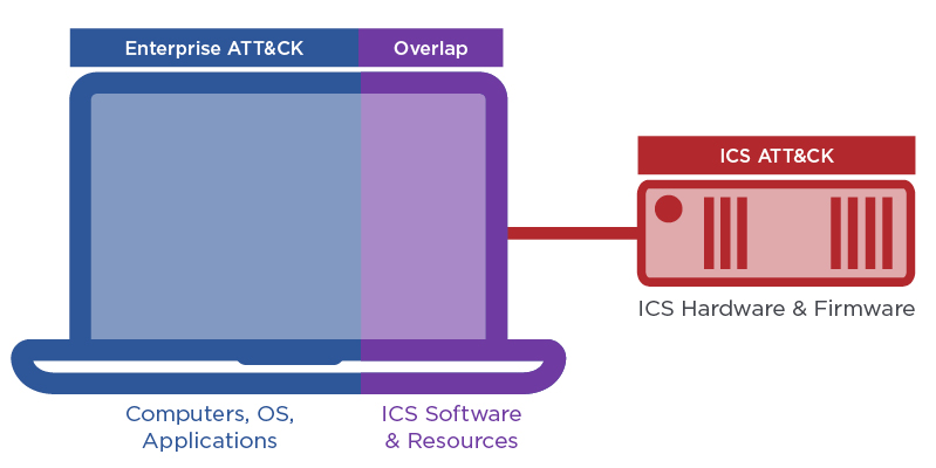
\includegraphics[width=0.9\textwidth]{img/attack-ICS.png}
    \caption{Endüstriyel Kontrol Sistemlerine (ICS) Yönelik Siber Saldırı Türleri}
    \label{fig:attack-ics}
\end{figure}

\subsection{ICS Taktikleri ve Teknikleri}

ATT\&CK for ICS, şu ana taktik kategorilerini içerir:

\begin{itemize}
\item \textbf{İlk Erişim (Initial Access):} Saldırganların ICS ağına ilk giriş yöntemleri.
\begin{itemize}
    \item Mühendislik İş İstasyonlarının Ele Geçirilmesi
    \item Dış Uzaktan Hizmetler
    \item İnternet Erişilebilir Cihaz
    \item Yeniden Satıcı/Tedarik Zinciri Ele Geçirme
\end{itemize}

\item \textbf{Keşif (Discovery):} ICS ortamını ve sistemlerini öğrenme teknikleri.
\begin{itemize}
    \item Kontrol Cihazı Keşfi
    \item I/O Modül Keşfi
    \item Seri Bağlantı Keşfi
    \item Program Organizasyon Birimi Keşfi
\end{itemize}

\item \textbf{Kalıcılık (Persistence):} Sistemde uzun süreli erişim sağlama yöntemleri.
\begin{itemize}
    \item Modül Firmware'i
    \item Sistem Firmware'i
    \item Proje Dosya Enfeksiyonu
\end{itemize}

\item \textbf{Yan Hareket (Lateral Movement):} ICS ağı içinde hareket etme teknikleri.
\begin{itemize}
    \item Programlama Yazılımı Kullanarak Erişim
    \item Uzak Hizmetler Üzerinden Hareket
    \item Veri Toplama Protokollerini Kötüye Kullanma
\end{itemize}

\item \textbf{Etki (Impact):} Sistemin işleyişini bozma veya kesintiye uğratma yöntemleri.
\begin{itemize}
    \item Kontrol Mantığının Değiştirilmesi
    \item Parametre Değişiklikleri
    \item Hizmet Kesintisi
    \item Güvenlik Enstrümantasyon Sisteminin Atlatılması
\end{itemize}
\end{itemize}

\subsection{ICS Savunma Stratejileri}

ATT\&CK for ICS çerçevesi, her teknik için karşı önlemler ve algılama yöntemleri önerir:

\begin{itemize}
\item \textbf{Ağ Segmentasyonu:} ICS ağının kurumsal ağdan ve internetten izole edilmesi.
\item \textbf{Erişim Kontrolü:} Sıkı erişim kontrol politikaları ve çok faktörlü kimlik doğrulama.
\item \textbf{Güvenlik İzleme:} ICS-spesifik anormallik tespiti ve olay izleme.
\item \textbf{Güvenlik Duvarları:} Endüstriyel protokolleri anlayan özelleştirilmiş güvenlik duvarları.
\item \textbf{Varlık Yönetimi:} Tüm ICS bileşenlerinin detaylı envanteri.
\end{itemize}

\subsection{Risk Değerlendirme ve Azaltma}

ICS güvenliği için risk değerlendirmesi, şu adımları içerir:

\begin{enumerate}
\item \textbf{Varlık Tanımlama:} Kritik ICS bileşenlerinin belirlenmesi.
\item \textbf{Tehdit Modelleme:} ATT\&CK for ICS kullanarak olası saldırı vektörlerinin belirlenmesi.
\item \textbf{Zafiyet Analizi:} Sistemdeki güvenlik açıklarının tespiti.
\item \textbf{Risk Değerlendirme:} Tehditlerin olasılık ve etki analizinin yapılması.
\item \textbf{Kontrol Seçimi:} Uygun güvenlik kontrollerinin belirlenmesi ve uygulanması.
\end{enumerate}

\section{Web Uygulama Güvenliği ve OWASP Framework}

Web uygulamaları, modern dijital ekosisteminde çok önemli bir role sahiptir ancak aynı zamanda siber saldırganların en çok hedeflediği varlıklar arasında yer alırlar. Web uygulama güvenliği, bu riskleri azaltmak ve kullanıcı verilerini korumak için hayati öneme sahiptir.

\subsection{OWASP Top 10 Zafiyetleri ve Azaltma Stratejileri}

Open Web Application Security Project (OWASP) Top 10, web uygulamalarındaki en kritik güvenlik risklerini listeleyen endüstri standardıdır. 2021 sürümü aşağıdaki tehditleri içermektedir:

\begin{enumerate}
\item \textbf{A01: Broken Access Control} - Erişim kontrolü zafiyetleri
\item \textbf{A02: Cryptographic Failures} - Kriptografik hatalar  
\item \textbf{A03: Injection} - Enjeksiyon saldırıları
\item \textbf{A04: Insecure Design} - Güvensiz tasarım
\item \textbf{A05: Security Misconfiguration} - Güvenlik yanlış yapılandırması
\item \textbf{A06: Vulnerable and Outdated Components} - Zafiyet bulunan bileşenler
\item \textbf{A07: Identification and Authentication Failures} - Kimlik doğrulama hataları
\item \textbf{A08: Software and Data Integrity Failures} - Yazılım ve veri bütünlüğü hataları
\item \textbf{A09: Security Logging and Monitoring Failures} - Güvenlik loglama ve izleme hataları
\item \textbf{A10: Server-Side Request Forgery (SSRF)} - Sunucu tarafı istek sahteciliği
\end{enumerate}

\subsection{Girdi Doğrulama, Çıktı Kodlama ve Parametreli Sorgular}

Güvenli web uygulama geliştirmenin temel prensipleri:

\begin{itemize}
\item \textbf{Girdi Doğrulama (Input Validation):} Tüm kullanıcı girdilerinin güvenilir olmadığı varsayılarak kapsamlı doğrulama yapılması
\item \textbf{Çıktı Kodlama (Output Encoding):} XSS saldırılarını önlemek için HTML, JavaScript ve CSS içeriğinin güvenli şekilde kodlanması
\item \textbf{Parametreli Sorgular (Parameterized Queries):} SQL enjeksiyonu saldırılarını önlemek için prepared statements kullanımı
\end{itemize}

\subsection{Kimlik Doğrulama ve Oturum Yönetimi Güvenliği}

Güvenli kimlik doğrulama ve oturum yönetimi için:

\begin{itemize}
\item Güçlü parola politikaları ve çok faktörlü kimlik doğrulama
\item Güvenli oturum token'ları ve uygun timeout değerleri
\item Session fixation ve session hijacking saldırılarına karşı koruma
\end{itemize}

\subsection{Cross-Site Scripting (XSS) ve Cross-Site Request Forgery (CSRF)}

\begin{itemize}
\item \textbf{XSS Koruması:} Content Security Policy (CSP), girdi doğrulama ve çıktı kodlama
\item \textbf{CSRF Koruması:} CSRF token'ları, SameSite cookie attribute kullanımı
\end{itemize}

\subsection{Content Security Policy (CSP) ve Güvenlik Header'ları}

Modern web uygulamalarında kullanılması gereken güvenlik header'ları:

\begin{itemize}
\item Content-Security-Policy
\item X-Frame-Options  
\item X-Content-Type-Options
\item Strict-Transport-Security
\item Referrer-Policy
\end{itemize}

\section{API Güvenliği ve Microservices Mimarisi}

API güvenliği, modern dağıtık sistemlerde kritik öneme sahiptir. Microservices mimarilerinin yaygınlaşmasıyla API güvenliği daha da kritik hale gelmiştir.

\subsection{RESTful API Güvenliği En İyi Uygulamaları}

\begin{itemize}
\item HTTPS kullanımı zorunluluğu
\item Uygun HTTP metod kullanımı
\item Rate limiting ve throttling
\item API versiyonlama güvenliği
\item Error handling ve bilgi sızıntısı önleme
\end{itemize}

\subsection{OAuth 2.0, OpenID Connect ve JWT Token Güvenliği}

Modern API kimlik doğrulama ve yetkilendirme standartları:

\begin{itemize}
\item OAuth 2.0 akışları ve güvenlik hususları
\item OpenID Connect identity layer implementasyonu
\item JWT token güvenliği: imzalama, şifreleme ve doğrulama
\item Token lifecycle yönetimi
\end{itemize}

\subsection{API Gateway Güvenlik Özellikleri ve Rate Limiting}

API Gateway'lerin güvenlik rolleri:

\begin{itemize}
\item Merkezi kimlik doğrulama ve yetkilendirme
\item Rate limiting ve DDoS koruması
\item Request/response transformation
\item API monitoring ve analytics
\end{itemize}

\subsection{GraphQL Güvenlik Hususları}

GraphQL'in getirdiği yeni güvenlik zorlukları:

\begin{itemize}
\item Query depth limiting
\item Query complexity analysis
\item Introspection devre dışı bırakma
\item Field-level authorization
\end{itemize}

\subsection{Microservices İletişim Güvenliği (mTLS, Service Mesh)}

Microservices arası güvenli iletişim:

\begin{itemize}
\item Mutual TLS (mTLS) implementasyonu
\item Service mesh güvenlik özellikleri (Istio, Linkerd)
\item Zero trust network principles
\item Service-to-service authentication
\end{itemize}

\section{Mobil Uygulama Güvenliği}

Mobil uygulama güvenliği, kullanıcı verilerini korumak ve yetkisiz erişimi önlemek için kritik öneme sahiptir. Mobil uygulamalar, hem cihazda hem de sunucu tarafında çeşitli güvenlik riskleriyle karşı karşıyadır. Bu riskler, veri sızıntıları, kötü amaçlı yazılım bulaşmaları ve kimlik avı saldırılarını içerir.

\subsection{iOS Uygulama Güvenliği: Kod İmzalaması, App Transport Security (ATS)}

\begin{itemize}
\item \textbf{Kod İmzalaması (Code Signing):} Bir iOS uygulamasının, Apple tarafından yetkilendirilmiş bir geliştirici tarafından imzalandığını doğrular. Bu imza, uygulamanın dağıtıldıktan sonra kurcalanmadığını ve değiştirilmediğini garanti eder.
\item \textbf{App Transport Security (ATS):} iOS 9 ve sonraki sürümler için varsayılan olarak etkin olan bir güvenlik özelliğidir. ATS, bir uygulamanın sunucuyla kurduğu tüm ağ bağlantılarının, minimum güvenlik gereksinimlerini (örn. TLS 1.2 veya daha yeni bir sürüm, güçlü anahtar boyutları) karşılayan güvenli bir TLS protokolüyle şifrelenmesini zorunlu kılar.
\end{itemize}
\subsection{Android Uygulama Güvenliği: ProGuard, Sertifika Sabitleme (Certificate Pinning)}
\begin{itemize}
\item \textbf{ProGuard:} Kod gizleme (obfuscation) ve optimizasyon aracıdır. Uygulamanın kodunu okunması ve tersine mühendislikle analiz edilmesi zor bir hale getirerek, fikri mülkiyetin korunmasına yardımcı olur. \texttt{build.gradle} dosyasında kolayca etkinleştirilebilir.
\item \textbf{Sertifika Sabitleme (Certificate Pinning):} Bir uygulamanın yalnızca belirli, önceden tanımlanmış sunucu sertifikalarına veya ortak anahtarlara güvenmesini sağlayan bir tekniktir. Bu, ortadaki adam (MITM) saldırılarına karşı güçlü bir savunma mekanizmasıdır. Ancak bu teknik, sunucu tarafındaki sertifika rotasyonu gibi durumlar için alternatif sabitleme (\texttt{pinset}) mekanizmalarıyla dikkatli bir şekilde yönetilmelidir.
\end{itemize}

\subsection{Mobil Uygulama Sızma Testi Metodolojileri}

Mobil uygulama sızma testi, uygulamadaki zafiyetleri bulmak için gerçek dünya saldırılarını simüle eder.

\begin{itemize}
\item \textbf{Statik Analiz:} Uygulama çalıştırılmadan kaynak kodu veya ikili dosyaları incelenir. Bu yöntem, sabit kodlanmış kimlik bilgileri ve güvensiz kodlama pratikleri gibi sorunları tespit eder.
\item \textbf{Dinamik Analiz:} Uygulama çalışırken, ağ trafiği, bellek kullanımı ve çalışma zamanı davranışı izlenir. Bu, çalışma zamanı zafiyetlerini (örn. güvensiz veri depolama, zafiyetli iletişim) ortaya çıkarır.
\item \textbf{En İyi Uygulamalar:} Mobil uygulama sızma testleri, OWASP Mobile Application Security Testing Guide (MASTG) gibi çerçeveler kullanılarak sistematik bir şekilde yürütülmelidir.
\end{itemize}
\subsection{Binary Koruma ve Anti-tampering Teknikleri}
\begin{itemize}
\item \textbf{İkili Koruma (Binary Protection):} Uygulama ikililerini tersine mühendislikten ve izinsiz değişikliklerden korumayı amaçlar.
\item \textbf{Anti-tampering:} Uygulamanın çalışırken veya statik haldeyken kurcalanmasını (değiştirilmesini) engellemek için tasarlanmış tekniklerdir.
\item \textbf{Teknikler:} Kod gizleme (obfuscation), dosya bütünlüğü kontrolü, hata ayıklama (debugger) algılama, jailbreak/root algılama gibi çeşitli yöntemler kullanılır.
\item \textbf{Savunma:} Statik (obfuscation, encryption) ve dinamik (RASP) önlemleri birleştiren çok katmanlı bir yaklaşım benimsenmelidir. RASP, çalışma zamanında kurcalama girişimlerini algılayıp yanıt vererek dinamik saldırılara karşı koruma sağlar.
\end{itemize}

\section{Web3 ve Blockchain Güvenliği}

Blockchain teknolojisi ve Web3 ekosistemin güvenliği, merkezi olmayan uygulamaların güvenli işlemesini sağlamak için kritik öneme sahiptir. Bu teknolojiler hem yenilikçi güvenlik özellikleri sunar hem de geleneksel güvenlik modellerinin ötesinde yeni zorluklar yaratır.

\subsection{Merkezi Olmayan Uygulamalar (DApps) Güvenliği}

Blockchain tabanlı uygulamaların güvenlik zorlukları ve korunma yöntemleri, geleneksel web uygulamalarından köklü farklılıklar gösterir. DApps, immutable (değiştirilemez) kod yapısı nedeniyle güvenlik açıklarının düzeltilmesini zorlaştırır.

\textbf{DApp Güvenlik Bileşenleri:}
\begin{itemize}
    \item \textbf{Smart Contract Layer:} İş mantığının çalıştığı katman
    \item \textbf{Frontend Interface:} Kullanıcı etkileşim katmanı  
    \item \textbf{Blockchain Network:} Altyapı ve consensus katmanı
    \item \textbf{Wallet Integration:} Kimlik doğrulama ve işlem imzalama
\end{itemize}

\textbf{Common DApp Security Risks:}
\begin{lstlisting}[breaklines=true,basicstyle=\ttfamily\footnotesize]
// Reentrancy saldırısından korunma örneği
pragma solidity ^0.8.0;

contract SecureDApp {
    mapping(address => uint256) private balances;
    bool private locked;
    
    modifier noReentrancy() {
        require(!locked, "Reentrant call");
        locked = true;
        _;
        locked = false;
    }
    
    function withdraw(uint256 amount) external noReentrancy {
        require(balances[msg.sender] >= amount, "Insufficient balance");
        
        // Checks-Effects-Interactions pattern
        balances[msg.sender] -= amount; // Effect önce
        
        (bool success, ) = msg.sender.call{value: amount}(""); // Interaction sonra
        require(success, "Transfer failed");
    }
}
\end{lstlisting}

\subsection{Smart Contract Güvenliği}

Akıllı sözleşmelerde karşılaşılan güvenlik açıkları ve audit süreçleri, blockchain ekosistemin güvenliğinin temelini oluşturur. Smart contract'lar immutable oldukları için güvenlik testleri dağıtımdan önce kritik önem taşır.

\textbf{Smart Contract Security Audit Process:}
\begin{enumerate}
    \item \textbf{Static Code Analysis:} Otomatik güvenlik tarama araçları (Slither, Mythril)
    \item \textbf{Manual Security Review:} Deneyimli auditörler tarafından kod incelemesi
    \item \textbf{Formal Verification:} Matematiksel doğrulama yöntemleri
    \item \textbf{Dynamic Testing:} Test ağlarında gerçek senaryo simülasyonları
\end{enumerate}

\textbf{Critical Smart Contract Vulnerabilities:}
\begin{itemize}
    \item \textbf{Reentrancy Attacks:} Fonksiyonun tamamlanmadan tekrar çağrılması
    \item \textbf{Integer Overflow/Underflow:} Sayısal taşma güvenlik açıkları
    \item \textbf{Access Control Issues:} Yetkilendirme kontrollerinin eksikliği
    \item \textbf{Front-running:} İşlem sıralamasını manipüle etme saldırıları
    \item \textbf{Flash Loan Attacks:} Anında borç mekanizmalarının kötüye kullanımı
\end{itemize}

\subsection{DeFi ve NFT Güvenlik Riskleri}

Merkezi olmayan finans (DeFi) ve NFT'lerdeki güvenlik sorunları, milyarlarca dolarlık varlığın risk altında olmasına neden olmaktadır.

\textbf{DeFi Security Architecture:}
\begin{lstlisting}[breaklines=true,basicstyle=\ttfamily\footnotesize]
// DeFi protocol güvenlik örneği
contract SecureDeFiProtocol {
    using SafeMath for uint256;
    
    // Price oracle manipulation koruması
    IPriceOracle[] public priceOracles;
    uint256 public constant ORACLE_DEVIATION_THRESHOLD = 5; // %5
    
    function getSecurePrice(address token) public view returns (uint256) {
        uint256[] memory prices = new uint256[](priceOracles.length);
        
        for (uint i = 0; i < priceOracles.length; i++) {
            prices[i] = priceOracles[i].getPrice(token);
        }
        
        // Median price calculation ve outlier detection
        uint256 medianPrice = calculateMedian(prices);
        validatePriceDeviation(prices, medianPrice);
        
        return medianPrice;
    }
    
    function validatePriceDeviation(uint256[] memory prices, uint256 median) 
        internal pure {
        for (uint i = 0; i < prices.length; i++) {
            uint256 deviation = prices[i] > median ? 
                prices[i].sub(median) : median.sub(prices[i]);
            uint256 deviationPercent = deviation.mul(100).div(median);
            
            require(deviationPercent <= ORACLE_DEVIATION_THRESHOLD, 
                    "Price oracle deviation too high");
        }
    }
}
\end{lstlisting}

\textbf{NFT Security Considerations:}
\begin{itemize}
    \item \textbf{Metadata Immutability:} NFT metadatalarının değiştirilemezliği
    \item \textbf{Royalty Bypass:} Telif hakkı ödemelerinin atlanması
    \item \textbf{Wash Trading:} Yapay fiyat manipülasyonu
    \item \textbf{Counterfeit NFTs:} Sahte NFT üretimi ve satışı
\end{itemize}

\subsection{Mobil Backend API Güvenliği Hususları}

Mobil uygulamalar, kullanıcı verilerini yönetmek ve iş mantığını yürütmek için arka uç API'leriyle iletişim kurar. Bu API'lerin güvenliği, en az mobil uygulama kadar kritik öneme sahiptir. Mobil backend API güvenliği, bu raporun Bölüm 4.3'te ele alınan genel API güvenliği ilkelerine dayanır. Bu, hem platformlar arası güvenlik tutarlılığını hem de savunmada derinlik prensibini pekiştirir. API'ler için TLS şifrelemesi, güçlü kimlik doğrulama, hız sınırlama ve API ağ geçidi kullanımı gibi uygulamalar, mobil ekosistemin bütünlüğünü korumada anahtar rol oynar.



\chapter{BULUT GÜVENLİĞİ VE KİMLİK ERİŞİM YÖNETİMİ}

\section*{Giriş}
Modern dijital dönüşümün kalbi olan bulut teknolojileri ve kimlik yönetimi sistemleri, günümüz siber güvenlik manzarasının en kritik bileşenlerindendir. Bu bölümde bulut güvenlik mimarileri, kimlik ve erişim yönetimi (IAM), sıfır güven modelleri ve modern kimlik doğrulama protokolleri gibi temel konular ele alınacaktır.

% Bulut güvenlik mimarisi diyagramı
\begin{figure}[h]
\centering
\includegraphics[width=0.8\textwidth]{img/cloud-security-architecture.png}
\caption{Modern Bulut Güvenlik Mimarisi ve Katmanları}
\label{fig:cloud-security-architecture}
\end{figure}

Modern bulut ortamları, geleneksel güvenlik yaklaşımlarının ötesinde yeni paradigmalar gerektirmektedir. Paylaşılan sorumluluk modeli, çoklu kimlik sağlayıcıları ve dinamik iş yükleri, güvenlik stratejilerinin de benzer şekilde adaptif ve kapsamlı olmasını zorunlu kılmaktadır.

\section{Bulut Güvenlik Mimarisi ve Paylaşılan Sorumluluk Modeli}

Bulut bilişim, kuruluşların altyapı yönetimi yükünü önemli ölçüde azaltırken, güvenlik yaklaşımında köklü bir değişikliği zorunlu kılmıştır. Geleneksel güvenlik modelleri, genellikle fiziksel veri merkezinin etrafına inşa edilen bir "çevre"yi korumaya odaklanırken, bulut ortamları dinamik ve dağınık yapısıyla yeni bir mimari ve sorumluluk çerçevesi gerektirir. Bu çerçeve, bulutun doğası gereği esneklik ve paylaşılan yetki alanları sunar ve bu nedenle güvenlik, yalnızca tek bir tarafın görevi olmaktan çıkmıştır.

\subsection{Bulut Güvenlik Mimarisi İlkeleri ve Referans Mimariler}

Bir bulut güvenlik mimarisi, bir kuruluşun buluta geçişle birlikte ortaya çıkan benzersiz güvenlik zorluklarından korunmasını sağlayan bir çerçevedir. Bu çerçeve, yalnızca teknolojik bileşenleri değil, aynı zamanda bu bileşenlerin nasıl tasarlanıp yönetileceğini belirleyen süreçleri ve ilkeleri de kapsar. Bulut güvenlik mimarisinin temel ilkeleri, riski yönetirken iş operasyonlarını kolaylaştırma dengesini gözetir.

Bu tasarımın temelinde yer alan ilkelerden biri otomasyondur. Bulut ortamlarının dinamik doğası ve hızlı ölçeklenebilme kapasitesi, güvenlik önlemlerinin manuel olarak uygulanmasını verimsiz ve hataya açık hale getirir. Güvenlik kontrollerinin ve dağıtımlarının otomasyonu, altyapı genişledikçe güvenlik önlemlerini ölçeklendirmek için temel bir gerekliliktir. Bu sayede güvenlik ekipleri tekrarlayan görevlerden kurtularak daha stratejik konulara odaklanabilir. Bir diğer kritik ilke ise derinlemesine savunma (Defense-in-Depth) yaklaşımıdır. Bu mimari prensip, tek bir güvenlik kontrolünün arızalanması durumunda sistemi koruyacak katmanlı kontrollerin uygulanmasını içerir. Bu, güvenlikte tek bir hata noktasını önlemeyi amaçlar. Son olarak, sıfır güven (Zero Trust) yaklaşımı, bir bulut güvenlik mimarisinin temel taşıdır. Bu model, ağ içindeki veya dışındaki hiçbir kullanıcıya ya da kaynağa peşin olarak güvenmez; bunun yerine, kimlik ve bağlama dayalı sürekli risk değerlendirmesi ve doğrulama gerektirir.

Bu ilkeler, AWS Güvenlik Referans Mimarisi (SRA) gibi somut kılavuzlarda uygulanmaktadır. AWS SRA, AWS Organizations kullanılarak çoklu hesap yapılarının nasıl güvenli hale getirileceğini gösterir. Bu, organizasyon genelinde güvenlik hizmetlerinin tutarlı bir şekilde nasıl uygulanacağına dair pratik bir yol haritası sunar. Ancak, bir referans mimarisi, her iş yükünün veya ortamın benzersiz tehdit maruziyetine göre tüm güvenlik hizmetlerini uygulamak zorunda olmadığını da belirtir. Bu, mimarinin katı kurallar bütünü yerine, riske dayalı ve duruma göre uyarlanabilir bir yaklaşım sergilemesi gerektiğini vurgular.

\subsection{Paylaşılan Sorumluluk Modeli: IaaS, PaaS, SaaS Güvenlik Sorumlulukları}

Bulut güvenliğinin en temel ve en sık yanlış anlaşılan kavramlarından biri Paylaşılan Sorumluluk Modeli'dir. Bu model, bulut sağlayıcısı (CSP) ve müşteri (CSC) arasında güvenlik görevlerinin net bir şekilde ayrıştırılmasını tanımlar. Temel ilke, sağlayıcının \textbf{"bulutun güvenliğinden"} (fiziksel altyapı, donanım, ağ) sorumlu olması, müşterinin ise \textbf{"buluttaki güvenlikten"} (veri, uygulamalar, yapılandırmalar) sorumlu olmasıdır. Bu ayrım, her bir bulut hizmet modeline (IaaS, PaaS, SaaS) göre farklılık gösterir ve güvenlik görevlerinin dağılımını belirler. Bu modelin doğru anlaşılması, potansiyel güvenlik risklerinin ele alınması, güvenlik duruşunun güçlendirilmesi ve ihlallere yol açabilecek yanlış anlamaların önüne geçilmesi için hayati önem taşır.

Hizmet modellerine göre sorumluluklar şu şekilde detaylandırılabilir:

\begin{itemize}
    \item \textbf{IaaS (Hizmet Olarak Altyapı):} AWS EC2 gibi IaaS hizmetlerinde müşteri, güvenlik görevlerinin çoğundan sorumludur. Bulut sağlayıcısı fiziksel altyapıyı yönetirken, müşteri işletim sistemi güncellemeleri, yama yönetimi, güvenlik grubu ve güvenlik duvarı yapılandırmaları, veri şifreleme ve IAM politikaları gibi görevleri üstlenmelidir. Bu modelde, müşteri kendi sanal veri merkezini yönetir.
    \item \textbf{PaaS (Hizmet Olarak Platform):} Microsoft Azure App Services gibi PaaS hizmetlerinde, bulut sağlayıcısı işletim sistemi, çalışma ortamı (runtime) ve ara katman yazılımları gibi bileşenlerin güvenliğini de sağlar. Müşterinin sorumluluğu, esas olarak kendi uygulamalarının ve bu uygulamalar içindeki verilerinin güvenliğine odaklanır.
    \item \textbf{SaaS (Hizmet Olarak Yazılım):} Microsoft 365 veya Google Workspace gibi SaaS hizmetlerinde, sağlayıcı yazılım, altyapı ve temel sistemler dahil olmak üzere neredeyse tüm güvenlik yönlerini yönetir. Müşteri, öncelikli olarak kimlik ve erişim yönetimini (IAM) ve verilerinin korunmasını sağlamalıdır.
\end{itemize}

Bu modelin en önemli çıkarımı, bulut sağlayıcısının kendi yükümlülüklerini yerine getirse bile, müşterinin tarafındaki yanlış yapılandırmaların veya zayıf erişim kontrollerinin ihlallere neden olabileceği gerçeğidir. Paylaşılan Sorumluluk Modeli, güvenlik boşluklarının önlenmesi, düzenleyici uyumluluğun sağlanması ve yasal yükümlülüğün azaltılması için kritik bir çerçevedir.

\begin{longtable}{|>{\scriptsize}p{1.1cm}|>{\scriptsize}p{1cm}|>{\scriptsize}p{1cm}|>{\scriptsize}p{1cm}|}
\caption{Paylaşılan Sorumluluk Modeli: Hizmet Modellerine Göre Sorumluluk Dağılımı}
\label{tab:shared_responsibility_model}\\
\hline
	extbf{Görev} & \textbf{IaaS} & \textbf{PaaS} & \textbf{SaaS}\\
\hline
\endfirsthead
\multicolumn{4}{c}%
{\tablename\ \thetable{} -- devamı}\\
\hline
\textbf{Güvenlik Görevi} & \textbf{IaaS (EC2)} & \textbf{PaaS (Azure)} & \textbf{SaaS (M365)}\\
\hline
\endhead
\hline
\multicolumn{4}{|r|}{Devamı bir sonraki sayfada}\\
\hline
\endfoot
\hline
\endlastfoot
Fiziksel Altyapı ve Tesis Güvenliği & Bulut Sağlayıcısı & Bulut Sağlayıcısı & Bulut Sağlayıcısı \\
\hline
Donanım, Yazılım ve Ağ & Bulut Sağlayıcısı & Bulut Sağlayıcısı & Bulut Sağlayıcısı \\
\hline
İşletim Sistemi ve Sanallaştırma & Müşteri & Bulut Sağlayıcısı & Bulut Sağlayıcısı \\
\hline
Uygulamalar ve Ara Katman Yazılımları & Müşteri & Müşteri & Bulut Sağlayıcısı \\
\hline
Kimlik ve Erişim Yönetimi (IAM) & Müşteri & Müşteri & Müşteri \\
\hline
Veri ve Şifreleme & Müşteri & Müşteri & Müşteri \\
\hline
Yapılandırma Yönetimi & Müşteri & Müşteri & Müşteri \\
\hline
\end{longtable}

\subsection{Çoklu-Bulut ve Hibrit Bulut Güvenlik Stratejileri}

Modern işletmeler, adaptasyon yetenekleri ve maliyet etkinliği gibi nedenlerle çoklu bulut ve hibrit bulut ortamlarını benimsemektedir. Ancak, bu stratejiler güvenlik yönetimini karmaşıklaştırır ve görünürlük eksikliği gibi zorlukları beraberinde getirir. Çoklu bulut güvenliği, birden fazla bulut ortamında tutarlı görünürlük, politika ve yönetişim sağlamak için tek bir yönetim noktasını kullanan bir yaklaşımdır.

Etkili bir çoklu ve hibrit bulut güvenlik stratejisi oluşturmak için izlenmesi gereken adımlar şunlardır:
\begin{enumerate}
    \item \textbf{Paylaşılan Sorumluluk Modelini Anlamak:} Her bir bulut sağlayıcısının farklı sorumluluk seviyelerine sahip olabileceğini kavramak önemlidir. Bu, güvenlik boşluklarını önlemek için ek önlemlerin nerede uygulanması gerektiğini belirlemeye yardımcı olur.
    \item \textbf{Kapsamlı Bir Güvenlik Politikası Uygulamak:} Veri merkezleri ve tüm bulut ortamları arasında uçtan uca, tutarlı bir güvenlik politikası uygulanmalıdır. Bu politikalar, şifreleme, erişim kontrolü ve uygulama katmanı güvenliğini içermeli ve güncel en iyi uygulamaları yansıtacak şekilde düzenli olarak gözden geçirilmelidir.
    \item \textbf{Merkezi Görünürlük ve Kontrolü Sürdürmek:} Etkili güvenlik yönetimi için merkezi izleme ve yönetim araçları hayati öneme sahiptir. Bu araçlar, tüm bulut ortamlarına gerçek zamanlı görünürlük sağlayarak güvenlik olaylarına hızlı yanıt verilmesini mümkün kılar. Çoklu bulut ortamlarının dağınık yapısı, merkezi bir bulut güvenlik aracı olmadan yönetişim ve görünürlük zorlukları yaratır.
    \item \textbf{En Az Ayrıcalık Prensibini Uygulamak:} Kimlik ve erişim yönetimini (IAM) merkezi bir stratejiyle yönetmek, her bir bulut hizmet sağlayıcısının farklı kimlik doğrulama ve yetkilendirme protokollerini kullanması sorununu hafifletir. Bu, tüm altyapı genelinde tutarlı bir şekilde en az ayrıcalık erişimi politikalarının otomatik olarak uygulanmasını sağlar.
\end{enumerate}

\subsection{Bulut Güvenlik Çerçeveleri: Cloud Security Alliance (CSA) ve NIST Uygulamaları}

Bulut güvenliğindeki standartlaşma ve yönetişim, CSA ve NIST gibi kuruluşların sağladığı çerçeveler aracılığıyla sağlanır. Bu çerçeveler, kuruluşların bulut güvenliğini sistematik bir yaklaşımla ele almasını, uyumluluk gereksinimlerini karşılamasını ve risk temelli bir güvenlik duruşu oluşturmasını destekler.

\begin{itemize}
    \item \textbf{Cloud Security Alliance (CSA) Cloud Controls Matrix (CCM):} CSA CCM, bulut bilişim için tasarlanmış bir siber güvenlik kontrol çerçevesidir. 17 alanda 197 kontrol hedefinden oluşur ve bulut tedarik zincirindeki hangi güvenlik kontrollerinin hangi aktör tarafından uygulanması gerektiği konusunda rehberlik sunar. CCM, kuruluşların ISO, NIST ve PCI DSS gibi çoklu güvenlik standartlarına uyum sağlamasına yardımcı olarak süreci kolaylaştırır. CCM'in farklı standartlara eşleşmesi, sektörde güvenlik ve uyumluluk için tek bir dil oluşturma çabasını ortaya koyar. Bu, bulut güvenliğinin artık sadece bir teknoloji sorunu olmaktan çıkıp, uyumluluk ve yönetişim odaklı bir iş stratejisine dönüştüğünün bir göstergesidir.
    \item \textbf{NIST Cloud Security Guidelines:} Ulusal Standartlar ve Teknoloji Enstitüsü (NIST), Federal Bilgi Güvenliği Yönetimi Yasası (FISMA) gibi federal yasalar kapsamında bilgi güvenliğine ilişkin standartlar ve yönergeler geliştirir. NIST Özel Yayın (SP) 800-53, ABD federal hükümet kurumları ve kritik altyapılar için gerekli güvenlik ve gizlilik kontrollerini belirler. Bu çerçeve, kuruluşların risk değerlendirmesi yapmasına, uygun güvenlik kontrollerini seçip uygulamasını sağlamasına ve güvenlik duruşunu sürekli olarak izlemesine olanak tanıyan sistematik bir yaklaşım sunar. NIST'in kılavuzları, bulut ortamlarında güvenlik tehditlerini sistemik olarak yönetmek ve düzenleyici gerekliliklere uyumu sağlamak için pratik adımlar sağlar.
\end{itemize}

Bulut güvenliğinde referans mimarilerinin ve belirli ürünlerin (örneğin Google Cloud) bu gibi çerçevelere (NIST) uygunluğunun vurgulanması, bu standartların artık yalnızca birer kılavuz değil, aynı zamanda pratik uygulamaların güvenilirliğini ve pazarlama değerini artıran birer unsur haline geldiğini gösterir.

\section{Bulut Altyapı Güvenliği ve Yönetişim}

Bulut altyapısının dinamik ve programlanabilir doğası, güvenliğin de benzer şekilde kodlanabilir ve otomatikleştirilebilir olmasını gerektirmektedir. Bu bölüm, bulut ortamlarının yapılandırmasını ve korunmasını yönetmek için kullanılan modern araç ve yöntemleri ele almaktadır. Odak noktası, insan hatasını azaltan ve tutarlılığı artıran otomasyon ve politika tabanlı yaklaşımlardır.

\subsection{Kod Olarak Altyapı (IaC) Güvenlik En İyi Uygulamaları}

Kod Olarak Altyapı (IaC), altyapının insan tarafından okunabilir kod dosyalarıyla tanımlanmasını ve yönetilmesini sağlar. Bu yaklaşım, güvenlik açısından, yapılandırma hatalarının daha dağıtım aşamasına gelmeden önce "sola kaydırılarak" (shift-left) tespit edilmesini mümkün kılar. IaC güvenliği, geleneksel manuel süreçlerdeki tutarsızlıkları ve hataları ortadan kaldırarak daha güvenli ve tutarlı bir altyapı oluşturur.


Güvenli bir IaC stratejisi için en iyi uygulamalar şunlardır:

\begin{enumerate}
    \item \textbf{Gizli Verilerin Koddan Ayrılması:} API anahtarları, parolalar veya jetonlar gibi gizli veriler asla doğrudan IaC dosyalarına gömülmemelidir. Bunun yerine, AWS Secrets Manager, Azure Key Vault veya HashiCorp Vault gibi özel gizlilik yönetimi araçları kullanılmalıdır. Bu araçlar, hassas verilerin koddan ayrı ve güvenli bir şekilde saklanmasını sağlar.
    \item \textbf{Sürüm Kontrolü ve Akran Denetimi Uygulaması:} Tüm altyapı kodları bir sürüm kontrol deposunda (örneğin Git) saklanmalı ve değişiklikler pull requestler aracılığıyla akran denetiminden geçirilmelidir. Bu, yanlış yapılandırmaların erken aşamada yakalanmasını ve birden fazla geliştiricinin güvenliği gözden geçirmesini sağlar.
    \item \textbf{CI/CD Ortamında Güvenlik Taramaları:} Geliştirme ve dağıtım süreçlerinin otomatikleştirildiği CI/CD hatlarına güvenlik tarama araçları entegre edilmelidir. \texttt{Checkov}, \texttt{tfsec} veya \texttt{cfn-lint} gibi statik analiz araçları, dağıtımdan önce güvenlik risklerini otomatik olarak tespit eder.
\end{enumerate}

\subsubsection*{Pratik Senaryo: \texttt{Checkov} ile Yanlış Yapılandırılmış Terraform Kodunun Analizi}

Bu senaryo, herkese açık erişime izin veren yanlış yapılandırılmış bir AWS S3 kovasını (bucket) tanımlayan bir Terraform dosyasının güvenlik denetimini göstermektedir.

\textbf{Adım 1: Güvenlik Açığı İçeren Terraform Dosyasını Oluşturma (\texttt{main.tf})}

Bu dosya, S3 kovası için genel erişim engelleme ayarlarını \texttt{false} olarak belirleyerek bir güvenlik açığı oluşturur.

\begin{verbatim}
resource "aws_s3_bucket" "example" {
  bucket = "my-insecure-bucket-12345"
}

resource "aws_s3_bucket_public_access_block" "example" {
  bucket = aws_s3_bucket.example.id
  block_public_acls = false
  block_public_policy = false
  ignore_public_acls = false
  restrict_public_buckets = false
}
\end{verbatim}

\textbf{Adım 2: \texttt{Checkov} ile Taramayı Çalıştırma}

Dosyayı kaydettikten sonra, terminalden aşağıdaki komut çalıştırılır:

\begin{verbatim}
checkov -f main.tf
\end{verbatim}
\textbf{Adım 3: Komut Satırı Çıktısının Analizi}

\texttt{Checkov} taraması, aşağıdaki gibi bir çıktı üreterek güvenlik açıklarını net bir şekilde gösterir:

\begin{verbatim}
Passed checks: 2, Failed checks: 4, Skipped checks: 0
Check: CKV_AWS_53: "Ensure S3 bucket has block public ACLS enabled" FAILED 
for resource: aws_s3_bucket_public_access_block.example. File: /main.tf:9-16.
Check: CKV_AWS_54: "Ensure S3 bucket has block public policy enabled" FAILED...
\end{verbatim}
Çıktı, \texttt{block\_public\_acls} ve \texttt{block\_public\_policy} gibi kritik güvenlik ayarlarının beklendiği gibi yapılandırılmadığını belirtir.
\textbf{Adım 4: Güvenlik Açıklarını Giderme}
Geliştirici, \texttt{main.tf} dosyasını \texttt{block\_public\_acls = true} ve \texttt{block\_public\_policy = true} olarak düzelterek güvenlik politikasını uygular. Bu basit düzeltme, kodun güvenli bir varsayılan duruma (secure-by-default) dönmesini sağlar. Bu pratik senaryo, IaC tarama araçlarının dağıtımdan önce güvenlik açıklarını nasıl yakaladığına dair somut bir örnek sunar.

\subsection{Bulut Güvenlik Duruşu Yönetimi (CSPM) Araçları}

Bulut Güvenlik Duruşu Yönetimi (CSPM), bulut ortamlarındaki yanlış yapılandırmaları ve uyumluluk ihlallerini sürekli olarak izlemek ve düzeltmek için kullanılan otomasyon tabanlı bir yaklaşımdır. CSPM araçları, güvenlik denetimini otomatikleştirmeleri sayesinde, bulut ortamlarının hızlı ölçeklenmesine ayak uydurabilir.

CSPM'nin temel işlevleri şunlardır:

\begin{enumerate}
    \item \textbf{API Entegrasyonu:} CSPM çözümleri, aracı (agent) gerektirmezler. Bunun yerine, bulut sağlayıcılarının API'lerine (AWS, Azure, GCP) bağlanarak envanter, yapılandırmalar ve denetim kayıtları gibi verilere erişirler. Bu aracısız yaklaşım, dağıtımı kolaylaştırır.
    \item \textbf{Yanlış Yapılandırma Tespiti:} CSPM araçları, bulut kaynaklarının yapılandırmalarını CIS Benchmarks veya PCI DSS gibi endüstri standartlarına ve düzenleyici çerçevelere göre denetleyen önceden tanımlanmış politikalarla gelir. Örneğin, herkese açık erişimi olan bir S3 kovası veya herkese açık bir Kubernetes uç noktası, bir yanlış yapılandırma olarak otomatik olarak raporlanır.
    \item \textbf{Risk Bağlamsallaştırması ve Önceliklendirme:} Gelişmiş CSPM çözümleri, riskleri bağlamsallaştırmak için tekil miskonfigürasyonların ötesine geçer. Zafiyetler, aşırı izinler ve aktif tehditler gibi ek bulguları bir araya getirerek olası saldırı yollarını ortaya çıkarır. Bu, güvenlik ekiplerinin binlerce uyarı içinde en kritik tehditlere odaklanmasını sağlar.
\end{enumerate}

CSPM araçları, pasif bir denetim mekanizması olmaktan çıkıp, siber riskleri aktif olarak önceliklendiren ve saldırı yollarını haritalayan akıllı platformlara dönüşmüştür. Bu evrim, güvenlik operasyonlarında reaktiflikten proaktifliğe doğru bir değişimi temsil etmektedir.

\subsection{Bulut İş Yükü Koruma Platformu (CWPP) Çözümleri}

Bulut İş Yükü Koruma Platformu (CWPP), sanal makineler, konteynerler ve sunucusuz fonksiyonlar gibi bulut iş yüklerini siber tehditlere karşı korumayı amaçlayan bir çözümdür. CWPP'ler genellikle bir CWPP/CSPM/CRD platformu olan daha geniş bir CNAPP'nin (Bulut Yerel Uygulama Koruma Platformu) bir alt kümesidir. CWPP'nin yükselişi, geleneksel güvenlik çözümlerinin modern bulut ortamlarının dinamik ve heterojen yapısını korumada yetersiz kaldığının bir kanıtıdır.

CWPP'nin temel yetenekleri, çok çeşitli bulut iş yükleri için kapsamlı bir koruma sağlar:

\begin{itemize}
    \item \textbf{Zafiyet Yönetimi:} CWPP, iş yüklerindeki zafiyetleri sürekli olarak değerlendirir ve CVE (Common Vulnerabilities and Exposures) veritabanları gibi kaynakları kullanarak risklerini önceliklendirir.
    \item \textbf{Çalışma Zamanı Koruması (Runtime Protection):} CWPP'ler, iş yükleri çalışırken onları korur. Bu, davranışsal analiz, makine öğrenimi ve imza tabanlı algılama gibi yöntemleri kullanarak gerçek zamanlı tehdit tespiti yapmayı içerir.
    \item \textbf{Yapılandırma Yönetimi:} CWPP'ler, CIS Benchmarks gibi endüstri standartlarına uygunluğu denetler ve güvenli yapılandırmaların uygulanmasına yardımcı olur.
    \item \textbf{CI/CD Entegrasyonu:} CWPP'ler, güvenlik geri bildirimini yazılım geliştirme yaşam döngüsünün (SDLC) erken aşamalarına entegre ederek "sola kaydırma" (shift-left) güvenlik uygulamalarını kolaylaştırır.
\end{itemize}

CWPP çözümleri, iş yüklerinin çok çeşitlilik göstermesi (VM'ler, konteynerler, sunucusuz) ve çoklu bulut ortamlarının karmaşıklığı nedeniyle tekil bir platformun tümünü korumasını gerekli kılmıştır.

\subsection{Bulut Erişim Güvenlik Aracısı (CASB) Uygulaması}

Bulut Erişim Güvenlik Aracısı (CASB), bulut hizmetleri (özellikle SaaS) ile kullanıcılar arasında bir güvenlik politika uygulama noktası görevi görür. CASB'ler, kuruluşlara bulut hizmetleri üzerindeki kontrolü geri verir ve görünürlük eksikliği, veri kaybı ve kötü amaçlı yazılım gibi riskleri ele alır.

Bir CASB'nin temel fonksiyonları şunlardır:

\begin{itemize}
    \item \textbf{Uygulama Görünürlüğü ve Kontrolü:} Çalışanların hangi bulut uygulamalarını kullandığını keşfeder ve onaylanmamış (Shadow IT) uygulamalara erişimi engeller. Bu, riskleri yöneterek üretkenliği güvenli bir şekilde sürdürmeye yardımcı olur.
    \item \textbf{Veri Kaybı Önleme (DLP):} Hassas verilerin bulut uygulamalarına yüklenmesini veya bu uygulamalardan sızdırılmasını engeller. Bu, hem depolanan (at-rest) hem de aktarılan (in-transit) veriler için politikalar belirlemeyi içerir.
    \item \textbf{Bulut Kötü Amaçlı Yazılım Koruması:} Onaylanmış bulut dosya depolama uygulamalarındaki kötü amaçlı yazılımları algılar ve kaldırır, enfekte olmuş dosyaların indirilmesini ve paylaşılmasını önler.
\end{itemize}

CASB, güvenlik hizmeti sınırı (SSE) mimarisinin temel bir parçasıdır ve güvenli erişim hizmeti sınırı (SASE) mimarisine doğru bir evrimde kritik rol oynar. Bu araçlar, modern, hibrit çalışma ortamlarında uzaktan çalışanlar için kurumsal ağ dışındaki bulut uygulamalarını güvenli hale getirmenin anahtarıdır.

\subsection{Çoklu Bulut Güvenlik Yönetimi ve Yönetişimi}

Çoklu bulut ortamları, farklı kimlik yönetim sistemlerini, API'leri ve güvenlik hizmetlerini bir araya getirir. Etkili bir yönetişim için merkezi bir bakış açısı şarttır. Her bir bulut sağlayıcısının kendine özgü bir güvenlik araç ve hizmet setine sahip olması, çoklu bulut ortamlarında tutarlılık sağlamayı zorlaştırır. Bu zorluk, CSPM, CWPP ve CASB gibi platformların ortaya çıkmasına neden olmuştur. Bu platformlar, farklı bulut ortamlarının üzerine bir "soyutlama katmanı" inşa ederek tek bir kontrol noktasından yönetişimi mümkün kılar. Bu, bulut güvenliğindeki en önemli mimari trendlerden biridir. Güvenlik, artık her bir bulut ortamında ayrı ayrı yönetilmesi gereken bir mesele değil, tüm ekosistemde tutarlılık gerektiren bir disiplin olarak ele alınmaktadır.

\section{Kimlik ve Erişim Yönetimi (IAM) Temelleri}

Kimlik ve Erişim Yönetimi (IAM), modern siber güvenliğin temel direğidir ve "doğru kişinin, doğru zamanda, doğru kaynaklara erişimini sağlama" prensibine dayanır. Günümüzde hibrit çalışma modelleri, bulut-first stratejiler ve çoklu cihaz kullanımı, geleneksel çevre tabanlı güvenlik modellerini geçersiz kılmıştır. IAM sistemleri, bu karmaşık ortamlarda güvenli erişimi sağlamanın yanı sıra, regulatory compliance (mevzuata uyum) ve risk yönetimi için de kritik öneme sahiptir.

\subsection{Geleneksel IAM vs. Modern Kimlik Yönetimi}

\textbf{Geleneksel IAM Modeli:}
Geleneksel IAM sistemleri, kurumsal ağ sınırları içinde çalışan, merkezi dizin hizmetleri (Active Directory gibi) tabanlı modellerdir. Bu sistemlerin temel özellikleri:

\begin{itemize}
    \item \textbf{Çevre Tabanlı Güvenlik:} Güvenliğin ağ çevresi kontrolüne dayandığı model
    \item \textbf{Statik Rol Atama:} Kullanıcılara önceden tanımlanmış rollerin atandığı sistem
    \item \textbf{Sınırlı Bağlam Farkındalığı:} Cihaz, konum, zamana dayalı dinamik risk değerlendirmesi eksikliği
    \item \textbf{On-Premises Odaklı:} Kurumsal ağ içindeki kaynaklara erişim önceliği
\end{itemize}

\textbf{Modern Kimlik Yönetimi:}
Modern IAM sistemleri, bulut-first, sıfır güven prensiplerine dayanan, bağlam farkında (context-aware) sistemlerdir:

\begin{itemize}
    \item \textbf{Kimlik-Merkezli Güvenlik:} Güvenliğin kullanıcı kimliği etrafında şekillendiği model
    \item \textbf{Dinamik Risk Değerlendirmesi:} Gerçek zamanlı risk analizine dayalı erişim kararları
    \item \textbf{Bağlamsal Kimlik Doğrulama:} Cihaz durumu, konum, davranış analizi tabanlı MFA
    \item \textbf{API-First Mimari:} Mikroservisler ve REST API'ler üzerinden entegrasyon
\end{itemize}

\subsection{IAM Bileşenleri ve Mimari}

Modern IAM mimarisi aşağıdaki temel bileşenlerden oluşur:

\textbf{1. Kimlik Sağlayıcı (Identity Provider - IdP):}
\begin{lstlisting}[breaklines=true,basicstyle=\ttfamily\footnotesize]
// Modern IdP entegrasyonu - SAML 2.0 ile SSO
public class SAMLIdentityProvider {
    private final X509Certificate signingCert;
    private final PrivateKey signingKey;
    
    public SAMLResponse generateAuthResponse(AuthenticationRequest request) {
        // 1. Kullanıcı kimlik doğrulama
        User user = authenticateUser(request.getUsername(), request.getCredentials());
        
        // 2. SAML assertion oluşturma
        Assertion assertion = createAssertion(user);
        assertion.setIssuer("https://company.idp.com");
        assertion.setSubject(user.getSubjectNameID());
        
        // 3. Attribute statements (rol, grup bilgileri)
        List<AttributeStatement> attributes = buildAttributeStatements(user);
        assertion.getAttributeStatements().addAll(attributes);
        
        // 4. Digital signature
        assertion.setSignature(signAssertion(assertion, signingKey));
        
        // 5. SAML Response oluşturma
        Response response = new Response();
        response.getAssertions().add(assertion);
        
        return response;
    }
}
\end{lstlisting}

\textbf{2. Kimlik Deposu (Identity Store):}
\begin{itemize}
    \item \textbf{Active Directory:} Windows tabanlı ortamlarda merkezi kimlik yönetimi
    \item \textbf{LDAP:} Açık standart dizin protokolü
    \item \textbf{Cloud Directory Services:} Azure AD, AWS Directory Service, Google Cloud Identity
    \item \textbf{Database-Based:} İlişkisel veya NoSQL veritabanlarında kimlik bilgileri
\end{itemize}

\textbf{3. Yetkilendirme Motoru (Authorization Engine):}
\begin{lstlisting}[breaklines=true,basicstyle=\ttfamily\footnotesize]
// ABAC (Attribute-Based Access Control) motoru
public class ABACAuthorizationEngine {
    public AccessDecision evaluateAccess(AccessRequest request) {
        // 1. Konu (Subject) attributları
        Map<String, Object> subjectAttrs = getSubjectAttributes(request.getSubject());
        
        // 2. Kaynak (Resource) attributları  
        Map<String, Object> resourceAttrs = getResourceAttributes(request.getResource());
        
        // 3. Çevresel (Environmental) attributları
        Map<String, Object> envAttrs = getEnvironmentalAttributes();
        envAttrs.put("currentTime", LocalDateTime.now());
        envAttrs.put("sourceIP", request.getSourceIP());
        envAttrs.put("riskScore", calculateRiskScore(request));
        
        // 4. Policy evaluation engine
        return evaluatePolicies(subjectAttrs, resourceAttrs, envAttrs, request.getAction());
    }
    
    private double calculateRiskScore(AccessRequest request) {
        double riskScore = 0.0;
        
        // Coğrafi risk faktörü
        if (isHighRiskLocation(request.getSourceIP())) riskScore += 0.3;
        
        // Zaman tabanlı risk faktörü
        if (isOffHours(request.getTimestamp())) riskScore += 0.2;
        
        // Cihaz güven durumu
        if (!isTrustedDevice(request.getDeviceFingerprint())) riskScore += 0.4;
        
        // Davranışsal anomali
        if (detectAnomalousAccess(request)) riskScore += 0.5;
        
        return Math.min(riskScore, 1.0);
    }
}
\end{lstlisting>

\subsection{Çok Faktörlü Kimlik Doğrulama (MFA) ve Adaptive Authentication}

MFA, "bildiğin bir şey" (parola), "sahip olduğun bir şey" (token), "sen olan bir şey" (biyometrik) faktörlerinden en az ikisini gerektiren güvenlik mekanizmasıdır.

\textbf{Modern MFA Teknolojileri:}

\begin{tabularx}{\textwidth}{|l|X|X|X|}
\hline
\textbf{MFA Türü} & \textbf{Güvenlik Seviyesi} & \textbf{Kullanıcı Deneyimi} & \textbf{Uygulama Alanı} \\
\hline
\textbf{SMS/Voice} & Düşük (SIM swapping riski) & İyi & Tüketici uygulamaları \\
\hline
\textbf{TOTP (Authenticator Apps)} & Orta & İyi & Kurumsal uygulamalar \\
\hline
\textbf{Push Notifications} & Orta-Yüksek & Çok İyi & Mobil-first ortamlar \\
\hline
\textbf{FIDO2/WebAuthn} & Çok Yüksek & Mükemmel & Yüksek güvenlik gereksinimi \\
\hline
\textbf{Hardware Tokens} & Çok Yüksek & Orta & Kritik sistemler \\
\hline
\end{tabularx}

\textbf{Adaptive Authentication Örneği:}
\begin{lstlisting}[breaklines=true,basicstyle=\ttfamily\footnotesize]
// Risk tabanlı adaptive MFA
public class AdaptiveMFAEngine {
    public MFARequirement determineMFARequirement(LoginAttempt attempt) {
        RiskProfile riskProfile = calculateRiskProfile(attempt);
        
        if (riskProfile.getRiskScore() < 0.3) {
            // Düşük risk: Sadece password
            return MFARequirement.NONE;
        } else if (riskProfile.getRiskScore() < 0.7) {
            // Orta risk: SMS veya Authenticator App
            return MFARequirement.STANDARD_MFA;
        } else {
            // Yüksek risk: Hardware token veya biometric
            return MFARequirement.HIGH_ASSURANCE_MFA;
        }
    }
    
    private RiskProfile calculateRiskProfile(LoginAttempt attempt) {
        return RiskProfile.builder()
            .geolocationRisk(analyzeGeolocation(attempt.getSourceIP()))
            .deviceRisk(analyzeDeviceTrust(attempt.getDeviceFingerprint()))
            .behavioralRisk(analyzeBehavioralPattern(attempt.getUserId(), attempt))
            .temporalRisk(analyzeTemporalPattern(attempt.getTimestamp()))
            .build();
    }
}
\end{lstlisting}

\section{Konteyner ve Kubernetes Güvenliği}

Konteynerler ve Kubernetes, modern, bulut yerel (cloud-native) uygulamaların omurgasını oluşturmaktadır. Bu teknolojiler, hızlı geliştirme ve dağıtım döngüleri sağlarken, geleneksel güvenlik modellerinin karşılamadığı benzersiz güvenlik zorluklarını da beraberinde getirmektedir. Bu bölüm, konteyner ve Kubernetes yaşam döngüsünün her aşamasında güvenliğin nasıl sağlanacağını detaylandırmaktadır.

\subsection{Konteyner ve Sanallaştırma: Güvenlik Farklılıkları}

Sanal makinelerin (VM) aksine, konteynerler ana işletim sisteminin (host OS) çekirdeğini (kernel) paylaşır. Bu, bir konteynerdeki zafiyetin tüm ana sisteme veya diğer konteynerlere yayılması (container escape) riskini artırır. Konteynerler efemer (geçici) ve dinamik bir yapıya sahiptir; saniyeler içinde başlatılıp durdurulabilirler. Bu geçici yapı, statik güvenlik önlemlerinin yetersiz kalmasına neden olur ve sürekli izleme gereksinimini artırır.

\subsection{Konteyner İmaj Güvenliği ve Zafiyet Taraması}

Bir konteyner imajı, uygulama kodunu, çalışma zamanı ortamını ve bağımlılıkları içeren, salt okunur bir şablondur. İmaj güvenliği, uygulamanın çalışmaya başlamadan önce, yani geliştirme ve inşa aşamalarında güvenlik açıklarının taranmasını (shift-left) içerir.

\textbf{En İyi Uygulamalar ve Adımlar:}

\begin{enumerate}
    \item \textbf{Güvenilir Taban İmajı Kullanımı:} İmajlar, yalnızca Alpine veya Red Hat UBI gibi minimum boyutlu ve güvenilir taban imajlarından oluşturulmalıdır. Bu, potansiyel zafiyetleri ve saldırı yüzeyini azaltır.
    \item \textbf{Otomatik Tarama Entegrasyonu:} İmajlar, geliştirme döngüsünün (SDLC) erken aşamalarında, CI/CD hattına entegre edilmiş tarama araçlarıyla sürekli taranmalıdır. \texttt{Trivy}, \texttt{Grype} veya \texttt{Anchore} gibi araçlar, imajı bilinen zafiyetler (CVE) veritabanlarına göre analiz eder.
    \item \textbf{İmajların İmzalanması:} İmajların bütünlüğünü ve kimliğini doğrulamak için imza mekanizmaları kullanılmalıdır. Bu, kötü niyetli veya kurcalanmış imajların dağıtımını engeller.
\end{enumerate}

\subsection{Konteyner Çalışma Zamanı (Runtime) Güvenliği ve Davranışsal İzleme}

Çalışma zamanı (runtime) güvenliği, konteynerler aktif olarak çalışırken onları korumaya odaklanır. Statik güvenlik, imajları incelerken, çalışma zamanı güvenliği gerçek zamanlı olarak şüpheli davranışları izler ve tespit eder. Bu yaklaşım, derleme veya dağıtım aşamalarından kaçan tehditlere karşı kritik bir savunma katmanı sunar.

\textbf{Davranışsal İzleme Mekanizması:}
\begin{itemize}
    \item \textbf{Dinamik Taban Çizgisi:} Makine öğrenimi algoritmaları, normal uygulama davranışını (örneğin CPU kullanımı, ağ trafiği, dosya erişim kalıpları) öğrenir ve bu taban çizgisinden sapmaları (anomalileri) tespit eder. Bu yaklaşım, bilinmeyen veya sıfırıncı gün (zero-day) saldırılarını yakalamada özellikle etkilidir.
    \item \textbf{Tespit Edilen Tehdit Örnekleri:} Kötü amaçlı kod yürütme, ayrıcalık yükseltme saldırıları ve yapılandırma kayması (configuration drift) gibi tehditler bu yöntemle yakalanabilir. Örneğin, bir web sunucusu konteynerinin normalde bir kabuk (shell) başlatması veya hassas sistem dosyalarına erişmesi beklenmez. Davranışsal izleme, bu tür anormal aktiviteleri anında tespit ederek bir saldırı girişimi hakkında uyarı verir.
    \item \textbf{Önem:} Konteynerlerin ana sistem çekirdeğini paylaşması nedeniyle, bir ayrıcalık yükseltme saldırısı tüm ana sistemi tehlikeye atabilir. Bu nedenle, ayrıcalık değişikliklerini ve şüpheli sistem çağrılarını izlemek hayati önem taşır.
\end{itemize}

\subsection{Kubernetes Güvenliği: RBAC, Ağ Politikaları, Pod Güvenliği}

Kubernetes, konteyner orkestrasyonunun temel aracıdır. Güvenliği, küme katmanı, uygulama katmanı ve ağ katmanında çok yönlü bir yaklaşım gerektirir.

\begin{itemize}
    \item \textbf{Rol Tabanlı Erişim Kontrolü (RBAC):}
    \begin{itemize}
        \item \textbf{Teori:} RBAC, Kubernetes API'si ve küme kaynaklarına kimin (kullanıcılar, hizmet hesapları) erişebileceğini ve hangi eylemleri gerçekleştirebileceğini kontrol eder. En az ayrıcalık (Least Privilege) prensibini uygulamak için en temel mekanizmadır.
        \item \textbf{Uygulama (YAML Örneği):}
            \begin{itemize}
                \item Bir \texttt{Role} objesi, bir \texttt{namespace} içindeki izinleri tanımlar. 
                
                Aşağıdaki örnek, \texttt{default namespace}'indeki \texttt{pods} kaynaklarına \texttt{get}, \texttt{watch} ve \texttt{list} eylemlerini okuma yetkisi verir:
\begin{verbatim}
kind: Role
apiVersion: rbac.authorization.k8s.io/v1
metadata:
  namespace: default
  name: pod-reader
rules:
- apiGroups: [""]
  resources: ["pods"]
  verbs: ["get", "watch", "list"]
\end{verbatim}
                \item Bir \texttt{RoleBinding} objesi, tanımlanan \texttt{Role}'ü bir kullanıcıya veya hizmet hesabına atar. Aşağıdaki örnek, \texttt{pod-reader} rolünü \texttt{ci-bot} adlı bir \texttt{ServiceAccount}'a bağlar:
\begin{verbatim}
kind: RoleBinding
apiVersion: rbac.authorization.k8s.io/v1
metadata:
  name: read-pods
  namespace: default
subjects:
- kind: ServiceAccount
  name: ci-bot
  namespace: default
roleRef:
  kind: Role
  name: pod-reader
  apiGroup: rbac.authorization.k8s.io
\end{verbatim}
            \end{itemize}
    \end{itemize}
    \item \textbf{Ağ Politikaları (Network Policies):}
    \begin{itemize}
        \item \textbf{Teori:} Varsayılan olarak, Kubernetes'te podlar arasında sınırsız iletişim vardır. Ağ politikaları, podlar arası iletişimi kısıtlayarak saldırı yüzeyini azaltmaya yardımcı olur. Bu, hizmetleri mikro segmentlere ayırarak yanal hareket (lateral movement) riskini azaltır.
        \item \textbf{Uygulama (YAML Örneği):}
            \begin{itemize}
                \item Aşağıdaki örnek, yalnızca \texttt{access: true} etiketi olan podların, \texttt{app: nginx} etiketi olan bir servisle iletişim kurmasına izin veren bir ağ politikası tanımlar:
\begin{verbatim}
apiVersion: networking.k8s.io/v1
kind: NetworkPolicy
metadata:
  name: access-nginx
spec:
  podSelector:
    matchLabels:
      app: nginx
  ingress:
  - from:
    - podSelector:
        matchLabels:
          access: "true"
\end{verbatim}
            \end{itemize}
    \end{itemize}
    \item \textbf{Pod Güvenlik Standartları (PSS):} Pod Güvenlik Politikaları'nın (PSP) yerini alan PSS, podların güvenlik seviyelerini (ayrıcalıklı, temel, kısıtlı) tanımlayan önceden belirlenmiş bir yaklaşımdır. Bu, yöneticilerin podların güvenlik yapılandırmalarını daha basit ve tutarlı bir şekilde uygulamalarını sağlar.
\end{itemize}

\subsection{Servis Mesh Güvenliği (Istio, Linkerd) Uygulamaları}

Mikro hizmet mimarilerinde hizmetler arası iletişimi yönetmek için bir servis ağı (service mesh) kullanılır. Güvenlik açısından, bir servis ağı, sıfır güven (zero-trust) ilkelerini uygulama ve trafik güvenliğini yönetme için ideal bir platformdur.

\begin{itemize}
    \item \textbf{Temel Güvenlik Özellikleri:}
    \begin{itemize}
        \item \textbf{Karşılıklı TLS (mTLS):} Istio ve Linkerd, hizmetler arası tüm iletişimi otomatik olarak mTLS ile şifreler, bu da uygulama kodunda herhangi bir değişiklik yapmadan veri trafiğinin güvenliğini sağlar.
        \item \textbf{Politika Yönetimi:} Servis ağları, hizmetler arasında hangi iletişimin (örneğin, "X servisi sadece Y servisiyle konuşabilir") izin verildiğini tanımlayan politikalar oluşturulmasına olanak tanır.
    \end{itemize}
    \item \textbf{Istio vs. Linkerd Karşılaştırması:}
    \begin{itemize}
        \item \textbf{Istio:} Google, IBM ve Lyft tarafından geliştirilmiş olup, daha zengin bir özellik setine ve daha geniş bir ekosisteme sahiptir.
        \item \textbf{Linkerd:} Daha basit, daha hafif ve performansa odaklanmıştır. Ancak, bazı gelişmiş güvenlik ve trafik yönetimi özelliklerinden yoksundur ve yalnızca Kubernetes'i desteklemesi gibi sınırlamaları vardır.
    \end{itemize}
\end{itemize}
Servis ağları, ağ güvenliğini bir kodlama probleminden bir altyapı sorununa dönüştürür. Bu, güvenliğin bir yan görev olmaktan çıkıp, altyapı katmanında otomatik olarak uygulandığı, “kodla güvenlik” (security-as-as-code) trendinin bir parçasıdır.

\section{Sunucusuz Güvenlik ve Hizmet Olarak Fonksiyon (FaaS)}
Sunucusuz mimariler, altyapı yönetimini tamamen bulut sağlayıcısına bırakarak geliştirici çevikliğini artırır. Ancak, bu yeni model geleneksel güvenlik kontrollerinin öngöremediği benzersiz zorlukları beraberinde getirir.

\subsection{Sunucusuz Mimarideki Benzersiz Güvenlik Zorlukları}
\begin{itemize}
    \item \textbf{Genişleyen Saldırı Yüzeyi:} Sunucusuz bir uygulama, düzinelerce veya yüzlerce küçük fonksiyondan oluşabilir. Her bir fonksiyon, HTTP API'leri, veri depoları veya IoT cihazları gibi farklı olay kaynaklarından girdi alabilir. Bu, saldırı yüzeyini geleneksel uygulamalara göre önemli ölçüde artırır.
    \item \textbf{Aşırı Ayrıcalıklı Fonksiyonlar:} Fonksiyonlar arası etkileşimin karmaşıklığı nedeniyle, geliştiriciler bazen zaman baskısıyla fonksiyonlara ihtiyaç duyduklarından daha fazla izin verebilir. Bu durum, bir saldırganın tek bir zafiyeti kullanarak tüm sisteme yayılmasına olanak tanıyan bir güvenlik açığı oluşturur.
    \item \textbf{Olay Verisi Enjeksiyonu:} Kullanıcıdan gelen verilerin (örneğin, bir HTTP isteği gövdesi veya dosya adı) doğru şekilde doğrulanmadığı durumlarda, bir saldırgan kötü amaçlı kod enjekte edebilir. Sunucusuz mimaride, bu durum "olay enjeksiyonu" olarak adlandırılır ve uygulamanın beklenmeyen şekilde davranmasına neden olabilir.
    \item \textbf{"Denial of Wallet" (DoW) Saldırıları:} Sunucusuz modelde tüketim bazlı ödeme yapıldığından, bir saldırgan aşırı fonksiyon çağrımı yaparak veya fonksiyonları beklenenden daha uzun süre çalışmaya zorlayarak kuruluşun maliyetlerini artırabilir. Bu, DoS saldırılarının sunucusuz ortama özgü bir varyantıdır.
\end{itemize}

\subsection{Fonksiyon Düzeyi Güvenlik ve Kod Enjeksiyonu Önleme}
Fonksiyon düzeyindeki güvenlik, her bir fonksiyonu bağımsız bir güvenlik sınırı olarak ele alır. Kod enjeksiyonu, kullanıcı girdisinin güvenli bir şekilde işlenmemesinden kaynaklanan yaygın bir tehdittir.

\textbf{Pratik Yönergeler ve Örnekler:}
\begin{enumerate}
    \item \textbf{Giriş Doğrulama (Input Validation) ve Temizleme (Sanitization):} Tüm kullanıcı girdisi (form alanları, HTTP başlıkları, çerezler vb.) güvenilir kabul edilmemeli ve kullanılmadan önce doğrulanmalıdır.
    \begin{itemize}
        \item \textbf{Senaryo:} AWS Lambda'da bir Node.js fonksiyonu ile gelen JSON verisini doğrulama.
        \item \textbf{Adım 1:} Gelen veriyi (event body) doğrulamak için \texttt{jsonschema} gibi bir kütüphane kullanılabilir.
        \item \textbf{Adım 2:} Giriş verisinin beklenen yapıda olduğunu garanti eden bir JSON şeması oluşturun. Şema, gerekli alanları, veri tiplerini ve ek özelliklere izin verilip verilmeyeceğini tanımlar.
\begin{verbatim}
const schema = {
  "id": "/Order",
  "type": "object",
  "properties": {
    "order_id": {"type": "string"},
    "amount": {"type": "number"},
    "item": {"type": "string"}
  },
  "required": ["order_id", "amount", "item"],
  "additionalProperties": false
};
\end{verbatim}
        \item \textbf{Adım 3:} Gelen veriyi bu şemaya göre doğrulayın. Eğer doğrulama başarısız olursa, fonksiyonun yürütülmesini durdurun ve anlamlı bir hata mesajı döndürün. Örneğin, \texttt{amount} alanı sayı yerine bir metin olarak gelirse, \texttt{jsonschema} bir doğrulama hatası fırlatacaktır.
    \end{itemize}
    \item \textbf{Parametrelendirilmiş Sorgular:} SQL enjeksiyonunu önlemek için, kullanıcı girdilerini doğrudan SQL sorgularına eklemek yerine parametreli sorgular (prepared statements) kullanılmalıdır. Bu yöntem, girdiyi veri olarak değerlendirir ve çalıştırılabilir kod olarak yorumlamaz.
\end{enumerate}

\subsection{Olay Odaklı (Event-driven) Güvenlik ve Tetikleyici Doğrulaması}
Sunucusuz mimariler, bir veritabanında değişiklik yapılması veya bir S3 kovasına dosya yüklenmesi gibi olaylar tarafından tetiklenir. Güvenlik, bu olayların ve tetikleyicilerin güvenli bir şekilde doğrulanmasını gerektirir. Olay yönlendiricileri (event routers), olayları yayınlayabilecek ve onlara abone olabilecek kullanıcı ve kaynakları kısıtlamak için rol tabanlı erişim kontrolü (RBAC) politikaları uygulanabilir. Bu, güvenlik kontrollerinin geleneksel ağ topolojilerinden ziyade, veri akışına ve olay zincirlerine dayalı hale geldiğini göstermektedir. Bu mimari, bileşenler arasındaki bağımlılığı azaltarak uygulamaların daha esnek olmasını sağlar.

\subsection{Sunucusuz Uygulama İzleme ve Loglama}
Sunucusuz fonksiyonlar efemer (kısa ömürlü) ve durumsuzdur. Bu, geleneksel izleme ve loglamayı zorlaştırır, çünkü bir fonksiyonun yaşam süresi milisaniyeler olabilir ve bağlamı korumak zorlaşır.

\textbf{İzleme ve Loglama için Pratik Yaklaşımlar:}
\begin{itemize}
    \item \textbf{Merkezi Loglama:} Tüm fonksiyonların logları, bulut sağlayıcının (örneğin AWS CloudWatch, Google Cloud Logging) veya üçüncü parti bir izleme aracının merkezi bir loglama hizmetine gönderilmelidir.
    \item \textbf{Korelasyon Kimlikleri:} Asenkron çağrılan fonksiyonlar arasında aynı isteğe ait log girdilerini birleştirmek için korelasyon kimlikleri kullanılmalıdır. Bu, bir uygulamanın uçtan uca davranışını izlemeyi mümkün kılar.
    \item \textbf{Metrik İzleme:} Sunucusuz izleme çözümleri, fonksiyon sağlığı ve bellek kullanımı gibi metrikleri izleyerek, uygulama darboğazlarını ve maliyet sorunlarını belirlemeye yardımcı olur.
\end{itemize}
Sunucusuz ortamlar, "yüksek düzeyde gözlemlenebilirlik" (deep observability) ihtiyacını artırmıştır. Geleneksel log toplama yetersizdir; bir işlem akışının başlangıcından sonuna kadar tüm mikro hizmetleri ve olayları bağlamsal olarak izleyebilen araçlar zorunluluk haline gelmiştir. Bu, sunucusuz güvenliğin maliyet yönetimi ve performans optimizasyonuyla doğrudan ilişkili olduğu bir alandır.

\subsection{Sunucusuz Mimaride Üçüncü Parti Entegrasyon Güvenliği}
Sunucusuz uygulamalar genellikle üçüncü parti hizmetlere (örneğin, API'ler, veri tabanları, ödeme ağ geçitleri) entegre olur. Bu entegrasyonlar, potansiyel güvenlik riskleri taşır. Güvenliği sağlamak için aşağıdaki önlemler alınmalıdır:
\begin{itemize}
    \item \textbf{Sıkı Erişim Kontrolleri:} Üçüncü parti hizmetlere erişim için en az ayrıcalık ilkesi uygulanmalı, yalnızca gerekli izinler verilmelidir.
    \item \textbf{Gizli Veri Yönetimi:} API anahtarları gibi gizli veriler, kodun içine gömülmek yerine AWS Secrets Manager veya Azure Key Vault gibi özel gizlilik yönetimi hizmetlerinde saklanmalıdır.
    \item \textbf{Sürekli İzleme ve Loglama:} Üçüncü parti entegrasyonlarındaki anormal davranışlar, sürekli izleme ve loglama mekanizmalarıyla takip edilmelidir.
\end{itemize}

\section{Bulut Kimlik ve Erişim Yönetimi (CIAM)}
Kimlik ve erişim yönetimi (CIAM), bulut güvenliğinin temel direklerinden biridir. Bu bölüm, buluta özgü IAM modellerini, federasyon kavramını ve ayrıcalıklı erişim yönetimi gibi gelişmiş konuları ele alacaktır.

\subsection{Buluta Özgü Kimlik Sağlayıcıları (AWS IAM, Azure AD, GCP IAM) Karşılaştırması}
Üç büyük bulut sağlayıcısı da benzer hedeflere (kimin neye ve hangi koşullarda erişebileceğini kontrol etme) sahip olsa da, her birinin IAM çerçevesi kendi platform mimarisini ve felsefesini yansıtan benzersiz bir yapıya sahiptir. Bu farklılıkları anlamak, çoklu bulut ortamlarında güvenli ve yönetilebilir erişim kontrolleri tasarlamak için kritik öneme sahiptir.

\begin{longtable}{|>{\footnotesize}p{1.2cm}|>{\footnotesize}p{1.2cm}|>{\footnotesize}p{1.4cm}|>{\footnotesize}p{1.1cm}|}
\caption{Büyük Bulut Sağlayıcılarında Kimlik ve Erişim Yönetimi (IAM) Karşılaştırması}
\label{tab:iam_comparison}\\
\hline
\textbf{Özellik} & \textbf{AWS IAM} & \textbf{Azure IAM (Microsoft Entra ID)} & \textbf{GCP IAM}\\
\hline
\endfirsthead
\multicolumn{4}{c}%
{\tablename\ \thetable{} -- devamı}\\
\hline
\textbf{Özellik} & \textbf{AWS IAM} & \textbf{Azure IAM (Microsoft Entra ID)} & \textbf{GCP IAM}\\
\hline
\endhead
\hline
\multicolumn{4}{|r|}{Devamı bir sonraki sayfada}\\
\hline
\endfoot
\hline
\endlastfoot
Mimari Modeli & Düz ancak esnek bir yapı; politikalar doğrudan kullanıcı, grup veya rollere eklenir. Hassas ve ayrıntılı izinler sunar. & Geleneksel kurumsal yapılara benzer, dört katmanlı hiyerarşik model (Yönetim Grubu > Abonelik > Kaynak Grubu > Kaynak). & Basit hiyerarşik kaynak ağacı (Kuruluş > Klasör > Proje > Kaynak). İzinler bu ağaçta aşağı doğru akar. \\
\hline
Rol ve İlke Yönetimi & İzinleri tanımlayan JSON tabanlı politikalar (Policy) kullanılır. Politika Simülatörü ve Erişim Analiz Aracı gibi araçlarla yapılandırma hataları önlenir. & Rol Tabanlı Erişim Kontrolü (RBAC) ve yerleşik roller (örneğin Katkıda Bulunan, Okuyucu) kullanılır. Yetkilendirme için Koşullu Erişim politikaları uygulanabilir. & Üyelere (kullanıcılar, gruplar) bir kaynak üzerinde rol atayan "bağlantılar" (bindings) kullanılır. "IAM Koşulları" (Conditions) ile bağlama dayalı (zaman, IP vb.) izinler belirlenebilir. \\
\hline
Geçici Erişim Mekanizmaları & Geçici kimlik bilgileri için rollerin "üstlenilmesi" (assume role) mekanizması kullanılır. Bu, uzun süreli kimlik bilgilerine olan ihtiyacı azaltır. & Privileged Identity Management (PIM) hizmeti ile ayrıcalıklı erişim için just-in-time (JIT) erişim ve onay iş akışları sağlanır. & Belirli bir kapsamdaki izinlere sahip hizmet hesapları ve kısa ömürlü belirteçler (token) kullanılır. \\
\hline
Örnek Senaryo & Bir EC2 örneğine bir S3 kovasına erişmesi için belirli bir rol atanması. & Bir kullanıcının yalnızca belirli bir abonelik altındaki kaynak gruplarına kaynak dağıtma izninin verilmesi. & Bir projedeki tüm kullanıcıların, projenin altındaki tüm kaynaklara yalnızca okuma iznine sahip olması. \\
\hline
\end{longtable}

Bu üç platformun her birinin kendine özgü bir mimari ve yönetim modeline sahip olması, çoklu bulut ortamlarında tutarlı bir kimlik politikası oluşturmanın en büyük zorluklarından biridir. Bu durum, birleşik bir kimlik federasyonu stratejisini zorunlu kılmaktadır.

\subsection{Multi-Cloud Security Governance ve Cloud Security Mesh}

Modern kuruluşlar ortalama 3-4 farklı bulut sağlayıcısı kullanmaktadır. Bu çoklu bulut (multi-cloud) gerçekliği, güvenlik yönetişiminde yeni zorluklar yaratmaktadır.

\textbf{Cloud Security Mesh Architecture:}
Cloud Security Mesh, çoklu bulut ortamlarında tutarlı güvenlik politikaları uygulayan dağıtık güvenlik mimarisidir.

\begin{lstlisting}[breaklines=true,basicstyle=\ttfamily\footnotesize,language=Java]
// Multi-Cloud Security Orchestrator
public class MultiCloudSecurityOrchestrator {
    private final Map<CloudProvider, SecurityService> securityServices;
    private final UnifiedPolicyEngine policyEngine;
    private final CrossCloudIdentityFederation identityFed;
    
    public MultiCloudSecurityPosture assessSecurityPosture() {
        Map<CloudProvider, SecurityAssessment> assessments = new HashMap<>();
        
        for (CloudProvider provider : CloudProvider.values()) {
            SecurityService service = securityServices.get(provider);
            SecurityAssessment assessment = service.performSecurityAssessment();
            assessments.put(provider, assessment);
        }
        
        return MultiCloudSecurityPosture.builder()
            .providerAssessments(assessments)
            .crossCloudRisks(identifyCrossCloudRisks(assessments))
            .unifiedCompliance(assessUnifiedCompliance(assessments))
            .recommendedActions(generateUnifiedActions(assessments))
            .build();
    }
    
    public void enforceUnifiedSecurityPolicy(UnifiedSecurityPolicy policy) {
        // Translate unified policy to provider-specific policies
        for (CloudProvider provider : policy.getTargetProviders()) {
            ProviderSpecificPolicy providerPolicy = 
                policyEngine.translateToProviderPolicy(policy, provider);
            
            SecurityService service = securityServices.get(provider);
            service.deploySecurityPolicy(providerPolicy);
        }
        
        // Set up cross-cloud monitoring
        CrossCloudMonitor monitor = new CrossCloudMonitor(policy);
        monitor.startContinuousMonitoring();
    }
    
    private List<CrossCloudRisk> identifyCrossCloudRisks(
        Map<CloudProvider, SecurityAssessment> assessments) {
        
        List<CrossCloudRisk> risks = new ArrayList<>();
        
        // Check for inconsistent security policies
        if (hasInconsistentPolicies(assessments)) {
            risks.add(new CrossCloudRisk(
                RiskType.POLICY_INCONSISTENCY,
                "Security policies vary across cloud providers"
            ));
        }
        
        // Check for data governance gaps
        if (hasDataGovernanceGaps(assessments)) {
            risks.add(new CrossCloudRisk(
                RiskType.DATA_GOVERNANCE_GAP,
                "Data classification and protection inconsistent"
            ));
        }
        
        return risks;
    }
}
\end{lstlisting}

\textbf{Cloud-Native Security Architecture Patterns:}
\begin{itemize}
    \item \textbf{Security as Code:} Infrastructure security configurations managed through code
    \item \textbf{Immutable Infrastructure:} Security through infrastructure immutability
    \item \textbf{Defensive Architecture:} Defense-in-depth for cloud-native applications
    \item \textbf{Continuous Compliance:} Automated compliance monitoring and remediation
\end{itemize}

\subsection{Cloud Security Posture Management (CSPM) Advanced Implementation}

CSPM araçları, bulut altyapısının güvenlik duruşunu sürekli olarak değerlendirir ve iyileştirme önerileri sunar.

\textbf{Advanced CSPM Capabilities:}
\begin{lstlisting}[breaklines=true,basicstyle=\ttfamily\footnotesize]
// Advanced CSPM Engine
public class AdvancedCSPMEngine {
    private final CloudResourceInventory inventory;
    private final PolicyComplianceEngine complianceEngine;
    private final ThreatModelingEngine threatModeling;
    private final RemediationOrchestrator remediation;
    
    public CSPMAssessmentReport performAdvancedAssessment(CloudEnvironment environment) {
        // 1. Comprehensive Resource Discovery
        ResourceInventory resources = inventory.discoverAllResources(environment);
        
        // 2. Multi-Framework Compliance Assessment
        ComplianceResults compliance = complianceEngine.assessCompliance(
            resources,
            Arrays.asList(
                ComplianceFramework.CIS_BENCHMARK,
                ComplianceFramework.NIST_CSF,
                ComplianceFramework.SOC2,
                ComplianceFramework.ISO_27001
            )
        );
        
        // 3. Dynamic Threat Modeling
        ThreatModelResults threats = threatModeling.modelThreats(
            resources,
            environment.getArchitecturePatterns()
        );
        
        // 4. Risk Prioritization
        RiskPriorityMatrix risks = prioritizeRisks(compliance, threats);
        
        // 5. Automated Remediation Planning
        RemediationPlan remediation = this.remediation.planRemediation(risks);
        
        return CSPMAssessmentReport.builder()
            .resourceInventory(resources)
            .complianceStatus(compliance)
            .threatAssessment(threats)
            .riskPriority(risks)
            .remediationPlan(remediation)
            .securityScore(calculateSecurityScore(compliance, threats))
            .build();
    }
    
    public void executeAutomatedRemediation(RemediationPlan plan) {
        for (RemediationAction action : plan.getAutomatableActions()) {
            try {
                switch (action.getType()) {
                    case ENABLE_ENCRYPTION:
                        enableEncryptionAtRest(action.getTargetResource());
                        break;
                    case UPDATE_SECURITY_GROUPS:
                        updateSecurityGroupRules(action.getTargetResource(), action.getConfiguration());
                        break;
                    case ENABLE_LOGGING:
                        enableCloudTrailLogging(action.getTargetResource());
                        break;
                    case APPLY_TAGS:
                        applySecurityTags(action.getTargetResource(), action.getTagConfiguration());
                        break;
                }
                
                // Verify remediation success
                verifyRemediationSuccess(action);
                
            } catch (RemediationException e) {
                logRemediationFailure(action, e);
                escalateToSecurityTeam(action, e);
            }
        }
    }
}
\end{lstlisting}

\subsection{Serverless Security ve Function-as-a-Service (FaaS) Protection}

Serverless computing, yeni güvenlik paradigmaları ve zorlukları beraberinde getirmektedir.

\textbf{Serverless Security Challenges:}
\begin{itemize}
    \item \textbf{Function-Level Vulnerabilities:} Code injection, dependency vulnerabilities
    \item \textbf{Event-Driven Security:} Securing event triggers and data flows
    \item \textbf{Cold Start Security:} Initialization and bootstrap security
    \item \textbf{Shared Infrastructure Risks:} Multi-tenancy security concerns
\end{itemize}

\textbf{Serverless Security Framework:}
\begin{lstlisting}[breaklines=true,basicstyle=\ttfamily\footnotesize]
// Serverless Security Framework
public class ServerlessSecurityFramework {
    private final FunctionSecurityScanner functionScanner;
    private final EventSecurityValidator eventValidator;
    private final RuntimeProtection runtimeProtection;
    
    public ServerlessSecurityAssessment assessServerlessApplication(
        ServerlessApplication app) {
        
        // 1. Function Code Security Analysis
        List<FunctionSecurityIssue> codeIssues = functionScanner.scanFunctions(
            app.getFunctions()
        );
        
        // 2. Event Flow Security Validation
        List<EventSecurityIssue> eventIssues = eventValidator.validateEventFlows(
            app.getEventTriggers(),
            app.getDataFlows()
        );
        
        // 3. Runtime Security Configuration
        RuntimeSecurityConfig runtimeConfig = runtimeProtection.analyzeRuntime(
            app.getRuntimeConfiguration()
        );
        
        // 4. Dependency Security Assessment
        List<DependencyVulnerability> depVulns = assessDependencyVulnerabilities(
            app.getFunctionDependencies()
        );
        
        return ServerlessSecurityAssessment.builder()
            .functionIssues(codeIssues)
            .eventSecurityIssues(eventIssues)
            .runtimeConfiguration(runtimeConfig)
            .dependencyVulnerabilities(depVulns)
            .overallSecurityScore(calculateServerlessSecurityScore(codeIssues, eventIssues, depVulns))
            .build();
    }
    
    public void implementServerlessSecurityControls(ServerlessApplication app) {
        // 1. Function-level security
        for (ServerlessFunction function : app.getFunctions()) {
            implementFunctionSecurity(function);
        }
        
        // 2. Event security
        implementEventSecurity(app.getEventTriggers());
        
        // 3. Runtime protection
        deployRuntimeProtection(app);
    }
    
    private void implementFunctionSecurity(ServerlessFunction function) {
        // Input validation
        function.addInputValidation(createInputValidationRules(function));
        
        // Output sanitization
        function.addOutputSanitization(createOutputSanitizationRules(function));
        
        // Resource limits
        function.setResourceLimits(calculateSecureResourceLimits(function));
        
        // Environment security
        function.setEnvironmentSecurity(createSecureEnvironment(function));
    }
}
\end{lstlisting}

\subsection{Federasyon ve Tek Oturum Açma (SSO) Kavramları ve Uygulaması}
\begin{itemize}
    \item \textbf{Tanım:} Tek Oturum Açma (SSO), kullanıcıların tek bir kimlik bilgisi seti ile aynı etki alanı (domain) içindeki birden fazla uygulamaya erişmesini sağlar. Federasyon ise bu kavramı genişleterek, farklı etki alanları veya kuruluşlar (örneğin bir çalışan portalı ve üçüncü parti bir SaaS uygulaması) arasında bir güven ilişkisi kurar.
    \item \textbf{Nasıl Çalışır:} Bir kullanıcı, kimlik sağlayıcısına (IdP) bir kez oturum açtığında, IdP kullanıcıyı doğrular ve bir güvenlik onayı (assertion) gönderir. Hizmet sağlayıcısı (SP), bu onayı doğrulayarak kullanıcıya tekrar oturum açmasına gerek kalmadan erişim izni verir. Bu süreç, SAML, OAuth ve OpenID Connect gibi standart protokollerle mümkün olur.
    \item \textbf{Faydaları:} Federasyonun ana değeri, farklı kuruluşlar arasında iş birliğini basitleştirmesi ve IT ekiplerinin harici hizmetler için manuel hesap yönetimi yükünü azaltmasıdır. Bu, özellikle çoklu bulut ve SaaS uygulamalarının yaygınlaştığı bulut çağında tedarik zinciri güvenliği için kritik bir adımdır.
\end{itemize}

\subsection{Bulut Ortamlarında Ayrıcalıklı Erişim Yönetimi (PAM)}
Ayrıcalıklı Erişim Yönetimi (PAM), kuruluşları siber tehditlere karşı korumak için kritik kaynaklara (root hesaplar, yöneticiler, veritabanları vb.) ayrıcalıklı erişimi izleyen, tespit eden ve engelleyen bir kimlik güvenliği çözümüdür.

\begin{itemize}
    \item \textbf{Modern PAM Yaklaşımları:}
    \begin{itemize}
        \item \textbf{En Az Ayrıcalık (Least Privilege):} Bir kullanıcıya veya sürece, görevini yerine getirmesi için kesinlikle gerekli olan en az ayrıcalık verilmelidir.
        \item \textbf{Sıfır Duran Ayrıcalık (Zero Standing Privileges) ve Just-in-Time (JIT) Erişimi:} Kullanıcılara ayrıcalıklar kalıcı olarak verilmez. Bunun yerine, erişim yalnızca belirli bir süre (örneğin 1 saat) için, bir onay süreci veya gerekçe belirtme sonrasında dinamik olarak atanır. Azure'ın PIM (Privileged Identity Management) hizmeti, bu yaklaşımı uygulamak için bir örnek teşkil eder. Kullanıcılar, rolleri etkinleştirmek için istekte bulunur ve onaylandıktan sonra belirlenen süre boyunca bu role sahip olurlar. Süre dolduğunda, ayrıcalık otomatik olarak iptal edilir.
    \end{itemize}
    \item \textbf{Pratik Yönergeler:}
    \begin{itemize}
        \item \textbf{Çok Faktörlü Kimlik Doğrulama (MFA):} Tüm ayrıcalıklı hesaplar için MFA zorunlu hale getirilmelidir. Bu, kimlik bilgilerinin çalınması durumunda bile ek bir güvenlik katmanı sağlar.
        \item \textbf{Otomasyon:} Erişim ve yetkilendirme süreçlerini otomatikleştirmek, insan hatası riskini azaltır ve verimliliği artırır.
        \item \textbf{Sürekli İzleme ve Denetim:} Ayrıcalıklı hesap faaliyetleri sürekli olarak izlenmeli ve anormallikleri tespit etmek için denetlenmelidir.
    \end{itemize}
\end{itemize}
Bulut ortamlarında PAM, geleneksel on-premise çözümlerden daha güvenli olabilir. Otomatik parola döndürme, MFA ve JIT erişim mekanizmaları, insan hatası riskini azaltır ve saldırganların çalınan kimlik bilgilerini kullanmasını engeller.

\subsection{Kimlik Yönetişimi ve Otomatik Sağlama (Provisioning)}
\begin{itemize}
    \item \textbf{Tanım:} Kimlik yönetişimi, kimlik ve erişim haklarının, politikalar ve iş kurallarıyla uyumlu olmasını sağlar. Otomatik sağlama, yeni kullanıcılara veya rol değişikliklerine göre erişim haklarının otomatik olarak atanması veya kaldırılması sürecidir.
    \item \textbf{Faydaları:}
    \begin{itemize}
        \item \textbf{Gelişmiş Güvenlik:} Manuel süreçlerdeki hataları ve gözden kaçan güvenlik ayarlarını ortadan kaldırır.
        \item \textbf{Hızlı Eşleme ve İşten Çıkarma:} Yeni çalışanlara ihtiyaç duydukları erişimi ilk günden itibaren sağlar, aynı zamanda işten ayrılanların erişimini otomatik olarak kaldırarak "sahipsiz hesap" (orphaned accounts) riskini en aza indirir.
        \item \textbf{Etkili Uyumluluk ve Denetim:} Sağlama faaliyetlerine ilişkin detaylı denetim kayıtları (audit logs) oluşturarak, düzenleyici gerekliliklere uyumu kolaylaştırır.
    \end{itemize}
\end{itemize}
Otomatik sağlama, PAM ve SSO gibi teknik kontrollerin etkili bir şekilde çalışması için gerekli operasyonel altyapıyı sağlar. Kimlik ve erişim yönetiminin güvenliğini ve uyumluluğunu en üst düzeye çıkarmak için teknik kontroller ile operasyonel süreçlerin entegrasyonu şarttır. Bu, "güvenliğin bir ürün olmadığı, bir süreç olduğu" yönündeki temel ilkeyi destekler.

\section{Bulut Veri Koruma ve Şifreleme}
Veri, bulut bilişimin en değerli varlığıdır ve modern bulut güvenliğinin temelini oluşturur. Bu bölüm, verilerin yaşam döngülerinin farklı aşamalarında (durumda, aktarımda ve kullanımda) korunma stratejilerini ve anahtar yönetimi uygulamalarını ele almaktadır.

\subsection{Bulut Veri Sınıflandırma ve Etiketleme Stratejileri}
\begin{itemize}
    \item \textbf{Teori:} Veri sınıflandırması, verilerin hassasiyetine, gizliliğine ve iş üzerindeki etkisine göre kategorize edilmesidir. Bu, hangi verilerin daha yüksek düzeyde korunması gerektiğini belirleyen temel bir yönetişim adımıdır.
    \item \textbf{Faydaları:} Doğru sınıflandırma, erişim kontrolünü daha etkin yönetmeye, şifreleme politikalarını zorunlu kılmaya ve düzenleyici uyumluluğu sağlamaya yardımcı olur.
    \item \textbf{Pratik Adımlar:}
    \begin{enumerate}
        \item \textbf{Hedeflerin Tanımlanması:} Sınıflandırmanın amacını belirleyin (uyumluluk, veri güvenliği vb.).
        \item \textbf{Paydaşların Katılımı:} Sadece IT değil, aynı zamanda uyumluluk, hukuk ve iş birimi yöneticilerini de sürece dahil edin.
    \item \textbf{Çerçevenin Geliştirilmesi:} Veri kategorilerini (örneğin \seqsplit{"Gizli," "Hassas," "Kamuya Açık"}) ve onlara atanan güvenlik kontrollerini içeren bir çerçeve oluşturun.
        \item \textbf{Otomasyonun Kullanımı:} Veri sınıflandırma ve etiketleme süreçlerini otomatik hale getirmek için teknolojiden yararlanın.
    \end{enumerate}
\end{itemize}
Veri sınıflandırması, teknolojik bir kontrol olmaktan çok, güvenlik stratejilerini yönlendiren bir yönetişim aracıdır. Doğru bir sınıflandırma, en az ayrıcalık, şifreleme ve veri kaybı önleme (DLP) gibi diğer güvenlik mekanizmalarının etkin bir şekilde uygulanabilmesi için temel ön koşuldur.

\subsection{Bulut Şifrelemesi: Durumda, Aktarımda, Kullanımda}
Veri şifrelemesi, bir veri güvenliği stratejisinin en önemli bileşenidir. Verinin, yaşam döngüsünün her aşamasında şifrelenmesi gerekir.
\begin{itemize}
    \item \textbf{Durumda Şifreleme (At-rest):} Veri depolama ortamında (sabit disk, veritabanı, yedekleme) hareketsizken şifrelenmesidir. Bulut sağlayıcıları genellikle bu tür verileri varsayılan olarak şifreler.
    \item \textbf{Aktarımda Şifreleme (In-transit):} Veri, bir konumdan diğerine taşınırken şifrelenmesidir. Bu genellikle TLS (Transport Layer Security) veya mTLS gibi protokollerle sağlanır. Bu, verinin ağ üzerinde ele geçirilse bile okunamamasını sağlar.
    \item \textbf{Kullanımda Şifreleme (In-use):} Veri, işlem yapılırken, bellekte veya işlemci önbelleğinde şifrelenir. "Gizli Bilişim" (Confidential Computing) gibi yeni teknolojiler bu alana odaklanmaktadır.
\end{itemize}
Bulut sağlayıcıları varsayılan şifreleme sunsa da, bir uzman için bunun her zaman yeterli olmadığını anlamak önemlidir. Özellikle düzenleyici uyumluluk gereksinimleri (örneğin HIPAA, PCI DSS), müşteri tarafında ek şifreleme katmanlarının uygulanmasını zorunlu kılabilir.

\subsection{Bulut Anahtar Yönetim Hizmeti (KMS) Uygulaması}
KMS, şifreleme anahtarlarının yaşam döngüsünü (oluşturma, rotasyon, devre dışı bırakma, yok etme) merkezi olarak yönetmeyi sağlayan bir bulut hizmetidir. KMS, Paylaşılan Sorumluluk Modeli'nin doğrudan bir uzantısıdır. Sağlayıcı KMS hizmetini sunarken, anahtarların politikalarını ve yönetimini kontrol etmek müşterinin sorumluluğundadır.

\textbf{Anahtar Yönetim Yaklaşımları:}
\begin{itemize}
    \item \textbf{Bulut Tarafından Yönetilen Anahtarlar:} Bulut sağlayıcısı tarafından oluşturulan ve yönetilen anahtarlar, kolaylık ve düşük yönetim yükü sağlar.
    \item \textbf{Müşteri Tarafından Yönetilen Anahtarlar (CMEK):} Müşterinin kendi anahtarlarını yönetmesine olanak tanır. Bu, anahtar yaşam döngüsü üzerinde tam kontrol ve sorumluluk sağlar.
    \item \textbf{Harici Anahtar Yöneticileri (EKM):} Kuruluş, anahtarları bulut ortamı dışında yönetebilir. Bu, en yüksek düzeyde kontrol ve güven gerektiren durumlarda kullanılır.
\end{itemize}

\textbf{Pratik Yönergeler ve Örnekler (GCP KMS):}
\begin{itemize}
    \item \textbf{Adım 1: Keyring (Anahtar Halkası) Oluşturma:} Anahtarlar, mantıksal bir koleksiyon olan "keyring" içinde gruplandırılır.
\end{itemize}

\begin{lstlisting}[breaklines=true,basicstyle=\ttfamily\footnotesize]
gcloud kms keyrings create "my-keyring" --location "global"
\end{lstlisting}

\begin{itemize}
    \item \textbf{Adım 2: Şifreleme Anahtarı Oluşturma:} Şifreleme amacına yönelik bir anahtar oluşturulur.
\end{itemize}

\begin{lstlisting}[breaklines=true,basicstyle=\ttfamily\footnotesize]
gcloud kms keys create "my-key" --location "global" --keyring "my-keyring" --purpose "encryption"
gcloud kms keys create "my-key" \
    --location "global" \
    --keyring "my-keyring" \
    --purpose "encryption"
\end{lstlisting}

\begin{itemize}
    \item \textbf{Adım 4: Dosyayı Şifreleme Çözme:} Şifrelenmiş dosya aynı anahtar kullanılarak geri çözülür.
\end{itemize}

\begin{lstlisting}[breaklines=true,basicstyle=\ttfamily\footnotesize]
gcloud kms decrypt \
    --ciphertext-file data.txt.enc \
    --plaintext-file data-decrypted.txt \
    --location "global" \
    --keyring "my-keyring" \
    --key "my-key"
\end{lstlisting}

\subsection{Veritabanı Şifrelemesi ve Şeffaf Veri Şifrelemesi (TDE)}
\begin{itemize}
    \item \textbf{Teori:} Şeffaf Veri Şifrelemesi (TDE), veritabanındaki hassas verileri, veritabanı dosyaları çalınsa bile okunamaz hale getirmek için şifreler. En önemlisi, veriler yetkili kullanıcı veya uygulama için "şeffaf" bir şekilde şifrelenip çözülür; yani uygulama kodunda herhangi bir değişiklik yapılmasına gerek kalmaz.
    \item \textbf{Uygulama:} TDE, bulut sağlayıcısının varsayılan depolama şifrelemesine ek bir katman olarak kullanılır ve özellikle PCI DSS gibi düzenlemelere uyum sağlamak için gereklidir. Örneğin, Google Cloud SQL for SQL Server, yerleşik TDE desteği sunar ve veritabanı birincil anahtarından oluşturulan bir sertifika ile verileri şifreler.
\end{itemize}

\subsection{Yedekleme Şifrelemesi ve Olağanüstü Durum Kurtarma Güvenliği}
\begin{itemize}
    \item \textbf{Teori:} Yedekleme, genellikle güvenlik kontrollerinin gözden kaçtığı bir aşamadır. Yedeklemeler de en az canlı veriler kadar hassastır ve saldırganlar için cazip bir hedeftir.
    \item \textbf{Pratik Yönergeler:} Yedekleme verileri, bulutta depolanırken her zaman şifrelenmelidir. Felaket kurtarma (DR) planları, şifrelenmiş verilerin geri yüklenmesi için gerekli anahtar yönetimi süreçlerini içermelidir. Veritabanı gibi point-in-time recovery (PITR) etkinleştirilmiş bir hizmette TDE sertifikası döndürüldüğünde, yeni bir yedek oluşturulması, sertifika kaybı durumunda geri yükleme riskini azaltmaya yardımcı olur.
\end{itemize}
Bulut ortamlarında uçtan uca veri koruması, yalnızca aktif sistemlerin değil, aynı zamanda yedekleme ve kurtarma mekanizmalarının da güvenliğini sağlamayı gerektirir. Bu, güvenlik planlamasının bir yaşam döngüsü yaklaşımıyla ele alınması gerektiğini göstermektedir.

\chapter{DONANIM VE FİZİKSEL GÜVENLİK}

Bu bölüm, donanım ve fiziksel güvenlik konularını kapsamaktadır.
% ...existing code...
    \begin{lstlisting}[breaklines=true,basicstyle=\ttfamily\footnotesize]
$ sudo sbsign --key MOK.priv --cert MOK.pem \
    "/boot/vmlinuz-$(uname -r)" \
    --output "/boot/vmlinuz-$(uname -r)-signed"
    \end{lstlisting}

Güvenliğin en temel ve en kritik katmanını, yani donanım güvenliğini ve fiziksel koruma sistemlerini derinlemesine incelemektedir. Yazılım ve ağ güvenliği, sağlam bir donanım temeli olmadan yetersiz kalır. Bu rapor, siber güvenlik uzmanları için tasarlanmış olup, sistemin bütünlüğünü ve gizliliğini donanım seviyesinde nasıl koruyacaklarını anlamaları için kapsamlı bir rehber sunmaktadır.

\section{Donanım Güvenliği Temelleri ve Güven Kökü (Hardware Security Fundamentals and Root of Trust)}

Donanım güvenliği, bir sistemin tüm güvenli operasyonlarının dayandığı sarsılmaz bir temel görevi görür. Bu katman, yazılım tabanlı saldırıların ötesine geçerek, bir cihazın fiziksel bütünlüğünü ve en kritik verilerinin güvenliğini sağlamak için özel olarak tasarlanmış bileşenleri içerir. Bu bileşenler, bir güven zincirinin başlangıç noktası olarak işlev görerek sistemin en alt katmanından itibaren güvenilir bir şekilde başlatılmasını garanti eder.

\subsection{Donanım Güvenlik Modülü (HSM) Mimarisi}

Bir Donanım Güvenlik Modülü (HSM), kriptografik anahtarlar gibi dijital sırları saklamak, yönetmek ve şifreleme/şifre çözme gibi kritik kriptografik işlevleri güvenli bir ortamda gerçekleştirmek için tasarlanmış fiziksel bir donanımdır. Bu modüller, genellikle bir eklenti kartı veya bir bilgisayar sunucusuna veya ağa doğrudan bağlanan harici bir cihaz şeklinde gelir. Temel mimarisi, bus probing veya fiziksel kurcalama gibi saldırıları önlemek amacıyla bir veya daha fazla güvenli kriptoişlemci çipi içerir.

Bir HSM'in en önemli güvenlik mekanizmalarından biri, kurcalanmaya karşı sunduğu koruma seviyesidir. Bu, üç ana kategoride incelenir: kurcalanma kanıtı (tamper evidence), kurcalanma direnci (tamper resistance) ve kurcalanmaya duyarlı tepki (tamper responsiveness). Kurcalanmaya duyarlı HSM'ler, fiziksel bir müdahale girişimi tespit ettiklerinde, içlerindeki anahtarları silme veya cihazı kullanılamaz hale getirme gibi yıkıcı eylemler gerçekleştirebilir. Bu seviyedeki koruma, Common Criteria (EAL4+) ve FIPS 140 gibi uluslararası güvenlik standartları ve sertifikasyonlar aracılığıyla doğrulanır. HSM'in bu fiziksel ve mantıksal koruma mekanizmaları, onu yazılım temelli saldırılara karşı neredeyse bağışık kılar.

Bu mimarinin en önemli faydası, bir uygulamanın hassas özel anahtarlarını bir web sunucusunun belleğinde açıkta bırakma riskini ortadan kaldırmasıdır. Kriptografik işlemler, verilerin saldırganlardan korunduğu HSM ortamı içinde gerçekleşir. Bu durum, HSM'nin sadece bir depolama alanı değil, aynı zamanda güvenli bir işlem birimi olarak işlev görmesini sağlar. Bir uygulamanın, HSM'nin iç işleyişine doğrudan erişimi olmadan anahtarları kullanabilmesi, anahtar hırsızlığı ve oltalama saldırıları gibi yaygın tehditlere karşı önemli bir savunma katmanı oluşturur.

HSM'ler, yüksek değerli anahtarları koruma ihtiyacı duyulan birçok alanda kullanılır. Öne çıkan kullanım alanları şunlardır:
\begin{itemize}
    \item \textbf{Açık Anahtar Altyapısı (PKI):} Kök sertifika yetkilisi (CA) anahtarları gibi en kritik anahtarları koruyarak tüm güven zincirinin bütünlüğünü garanti eder.
    \item \textbf{Ödeme Sistemleri:} Kredi ve ödeme kartı bilgilerini korumak için kullanılır ve Payment Card Industry Data Security Standards (PCI DSS) gibi endüstri standartlarına uyumu kolaylaştırır.
    \item \textbf{SSL Bağlantıları:} Asimetrik anahtar operasyonları için yüksek performans sunarak sunucu işlemcisi üzerindeki yükü hafifletir.
    \item \textbf{Blok Zinciri:} Özel anahtarların güvenliğini sağlayarak blok zinciri süreçlerinin bütünlüğünü korumada kritik bir rol oynar.
\end{itemize}
HSM'lerin bir sunucuya entegrasyonu genellikle PKCS\#11 gibi standart arayüzler aracılığıyla gerçekleşir. Bu, uygulamaların donanıma özgü kodlar yazmadan HSM'in işlevselliğini kullanmasına olanak tanır.

\subsection{Güvenilir Platform Modülü (TPM) ve Ölçülmüş Önyükleme (Measured Boot)}

Güvenilir Platform Modülü (TPM), bir bilgisayarın donanım ve yazılım bütünlüğünü doğrulamak ve korumak için tasarlanmış, anakarta yerleşik bir çiptir. TPM'in en temel işlevi, bir sistemin önyükleme süreci boyunca çeşitli bileşenlerin (firmware, bootloader, işletim sistemi çekirdeği) ölçümlerini, yani kriptografik hash'lerini, güvenli ve kurcalanmaya dayanıklı Platform Konfigürasyon Kayıtları (PCR) olarak bilinen yazmaçlarda saklamaktır.

Ölçülmüş önyükleme (measured boot) süreci, bu ölçümlerin nasıl alındığını tanımlar. Sistem her bir bileşeni çalıştırmadan önce, onun hash değerini alır. Bu hash değeri, o anki PCR değeriyle birleştirilerek yeni bir hash oluşturulur ve PCR'ye kaydedilir. Bu sürece "hash zincirlemesi" (hash-chaining) denir. Bu zincirleme mekanizması, önyükleme sürecinin herhangi bir noktasında yapılan en küçük bir değişikliğin bile (örneğin bir rootkit'in enjeksiyonu) zincirin sonraki tüm aşamalarındaki PCR değerlerini tamamen değiştirmesini sağlar. Bu, bir saldırganın kötü amaçlı kodu gizlice enjekte etmesini neredeyse imkansız hale getirir, çünkü sistemin güvenli durumu anında bozulacaktır.

Bu PCR değerleri, uzaktan doğrulama (remote attestation) için kritik bir rol oynar. Bir cihaz, mevcut "sağlıklı" durumunu kanıtlamak için, TPM tarafından imzalanmış PCR değerlerini içeren bir kanıtı (quote) uzaktaki bir Sağlık Doğrulama Hizmeti'ne (Health Attestation Service) gönderebilir. Hizmet, bu kanıtı önceden tanımlanmış bir "güvenli durum" politikasıyla karşılaştırır. Eşleşme sağlanırsa, cihazın donanım ve yazılım bütünlüğünün bozulmadığı, yani sistemin güvenli bir şekilde başlatıldığı kanıtlanmış olur.

Bir sistemde TPM ve HSM'nin rolleri birbirini tamamlayıcıdır. HSM, hassas anahtarlar için bir "güvenlik kasası" işlevi görürken, TPM bir platformun bütünlüğünü doğrulayan bir "güvenilir denetçi" görevi görür. Bir sistem, önyükleme sırasındaki bütünlüğünü bir TPM aracılığıyla kanıtlayarak, bir HSM'de depolanan kriptografik anahtarlara erişim için güvenilir bir ortam haline geldiğini kanıtlayabilir. Bu, anahtar yönetimi ve platform bütünlüğü arasında bir "güven köprüsü" kurarak modern donanım tabanlı güvenlik mimarilerinin temelini oluşturur.

\subsection{Donanım Güven Kökü (Hardware Root of Trust) ve Güvenli Önyükleme (Secure Boot) Süreci}

Donanım Güven Kökü (RoT), bir sistemin tüm güvenli operasyonlarının dayandığı temeldir. Donanım tabanlı bir RoT, yazılım tabanlı saldırılara karşı bağışık olduğu için en güvenli uygulamayı temsil eder ve kriptografik anahtarları içererek yazılım için bir güven temeli oluşturur.


Bu temel, bir "güven zinciri" (chain of trust) aracılığıyla tüm sisteme yayılır. Güven zinciri, her bir donanım ve yazılım bileşeninin, bir önceki bileşen tarafından dijital olarak imzalanmış ve doğrulanmış olmasını sağlayan bir yapıdır. Bu süreç, güvenin donanıma yazılmış ilk ve kurcalanamaz kod (genellikle bir ROM'daki Birincil Önyükleme Yükleyicisi) ile başlamasını sağlar. Bu, tüm zincirin "güvenilir çapası"dır. Zincir, esneklik sağlamak amacıyla tasarlanmıştır, çünkü donanımın her bir yazılım parçasını kendisi doğrulaması yerine, güveni bir sonraki katmana (örneğin, önyükleme yükleyicisine) devreder.

Güvenli Önyükleme (Secure Boot) süreci, bu güven zincirinin pratik bir uygulamasıdır. Bu, donanım kökünden başlayarak, önyükleme sürecinde yalnızca güvenilir ve dijital olarak imzalanmış yazılımların (UEFI firmware, bootloader, kernel) yüklenmesini sağlayan bir güvenlik standardıdır. Bu mekanizma, önyükleme sırasında firmware rootkit'leri ve bootkit'leri gibi kötü amaçlı yazılımların sisteme sızmasını engeller.

Bir Linux sisteminde UEFI Güvenli Önyükleme uygulamasının adımları şunlardır:

\begin{enumerate}
    \item \textbf{Gerekli Araçların Kurulumu:}
    \begin{lstlisting}[breaklines=true,basicstyle=\ttfamily\footnotesize]
$ sudo apt install openssl sbsigntool efitools mokutil shim-signed grub-efi-amd64-signed
    \end{lstlisting}

    \item \textbf{Özel Anahtar ve Sertifika Oluşturma:}
    \begin{lstlisting}[breaklines=true,basicstyle=\ttfamily\footnotesize]
$ sudo openssl req --new -x509 -newkey rsa:2048 -keyout MOK.priv -outform DER -out MOK.der -days 36500 -subj "/CN=ECI/"
    \end{lstlisting}

    \item \textbf{Çekirdeği İmzalama:}
    \begin{lstlisting}[breaklines=true,basicstyle=\ttfamily\footnotesize]
$ sudo sbsign --key MOK.priv --cert MOK.pem "/boot/vmlinuz-$(uname -r)" --output "/boot/vmlinuz-$(uname -r)-signed"
    \end{lstlisting}

    \item \textbf{Sertifikayı Kaydetme (Enrollment):}
    \begin{lstlisting}[breaklines=true,basicstyle=\ttfamily\footnotesize]
$ sudo mokutil --import MOK.der
    \end{lstlisting}

    \item \textbf{Durum Doğrulaması:}
    \begin{lstlisting}[breaklines=true,basicstyle=\ttfamily\footnotesize]
$ mokutil --sb-state
    \end{lstlisting}
\end{enumerate}
Bu adımlar, sistemin önyükleme sürecinin yalnızca yetkili yazılımları yüklemesini garanti eder.

\subsection{Çip Seviyesi Güvenlik Özellikleri ve Güvenli Enklavlar (Secure Enclaves)}

Çip seviyesi güvenlik, bir sistemin saldırı yüzeyini en aza indirmek için özel olarak tasarlanmış donanım bileşenlerini içerir. Bu bileşenlerden biri olan Güvenli Enklav (Secure Enclave), ana işlemciden izole edilmiş özel, güvenli bir alt sistemdir. Amacı, uygulama işlemcisinin çekirdeği tehlikeye atılsa bile hassas kullanıcı verilerini güvende tutmaktır.

Güvenli Enklav'ın mimarisi, kendi özel işlemcisi, şifrelenmiş belleği, güvenli önyüklemesi ve kurcalamaya dayanıklı bir yapısı sayesinde yüksek düzeyde izolasyon sağlar. Bir örnek olarak Apple'ın Secure Enclave'i, ana işlemcinin şifresiz belleği normal bir şekilde okuyup yazmasını sağlarken, dışarıdan herhangi bir gözlemcinin sadece şifrelenmiş ve doğrulanmış bellek içeriğini görmesini garantiler. Bu, verilerin aktarımı sırasında bile gizliliği korur.

Bu özel donanım, biyometrik verilerin (Face ID, Touch ID), şifrelerin, kriptografik anahtarların ve mobil ödemelerle ilgili kritik işlemlerin güvenli bir şekilde işlenmesi ve saklanması için kullanılır. Güvenli Enklavlar, güven kökü mimarisinin bir uzantısı olarak kabul edilebilir. Güvenli Önyükleme tüm platformun bütünlüğünü sağlarken, Güvenli Enklavlar bu güvenilir platform içinde bile daha yüksek bir izolasyon ve gizlilik sunar. Bu, saldırı yüzeyini yalnızca önyükleme sürecinde değil, tüm sistemin yaşam döngüsü boyunca küçültür ve ana işlemci çekirdeğinin güvenliği ihlal edilse bile kritik verilerin güvende kalmasını sağlar.

\subsection{Tedarik Zinciri Donanım Güvenliği ve Sahte Ürün Tespiti}

Tedarik zinciri güvenliği, bir cihazın ve bileşenlerinin orijinal olduğunu, üretim ve dağıtım aşamalarında kurcalanmadığını doğrulamayı amaçlayan kritik bir alandır. Güvenilirliği kanıtlanmamış teknolojilerin kullanılması, organizasyonlar için gizli güvenlik açıklarına ve risklere yol açabilir.

Donanım bütünlüğünü doğrulamak için, cihaz üreticileri her cihaza, cihazın kimliğine güvenli bir şekilde bağlı bir "eser" (artifact) yerleştirebilir. Bu eser, cihazın attributes'larını (özelliklerini) içerebilir ve orijinalliğini teyit etmek için kullanılabilir. Müşteri, bu eserin kaynağını ve orijinalliğini doğrulayarak cihazın gerçekliğini teyit edebilir. Benzer bir süreç, cihazlar operasyonel kullanımdayken periyodik bütünlük doğrulaması için de uygulanabilir. Bu, sahte veya değiştirilmiş donanımın tespit edilmesine yardımcı olur ve güvenli bir tedarik zincirinin sürdürülmesi için kritik bir adımdır.

\section{Donanım Yazılımı (Firmware) Güvenliği ve Düşük Seviyeli Sistem Koruması}
Donanım yazılımı (firmware), bir donanım aygıtının temel işlevlerini kontrol eden ve işletim sistemi ile donanım arasında bir köprü görevi gören yazılımdır. Firmware, genellikle bir aygıtın kalıcı belleğinde saklanır ve işletim sistemi başlatılmadan önce çalışır. Bu nedenle, firmware seviyesindeki bir güvenlik açığı, işletim sistemi seviyesindeki güvenlik kontrollerini atlatabilir ve tespit edilmesi zor, kalıcı bir tehdit oluşturabilir.

\subsection{UEFI/BIOS Güvenliği ve Güvenli Önyükleme Uygulaması}

UEFI (Unified Extensible Firmware Interface) Güvenli Önyükleme, bir cihazın yalnızca güvenilir ve dijital olarak imzalanmış yazılımları kullanarak önyükleme yapmasını sağlayan bir güvenlik standardıdır. Bu, saldırganların sistem yazılımını değiştirerek yetkisiz veya kötü amaçlı kod çalıştırmasını engeller.

Bir Linux sisteminde bu standardın uygulanması, kendi sertifikanızı oluşturmayı ve önyükleme bileşenlerini bu sertifikayla imzalamayı içerir. Aşağıdaki adımlar, bu sürecin bir örneğini sunar:

\begin{enumerate}
    \item \textbf{Gerekli Araçların Kurulumu:}
    \begin{lstlisting}[breaklines=true,basicstyle=\ttfamily\footnotesize]
$ sudo apt install openssl sbsigntool efitools mokutil shim-signed grub-efi-amd64-signed
    \end{lstlisting}
    Bu komut, güvenli önyükleme için gerekli olan tüm araçları kurar.
    \item \textbf{Özel Anahtar ve Sertifika Çifti Oluşturma:}
    \begin{lstlisting}[breaklines=true,basicstyle=\ttfamily\footnotesize]
$ sudo openssl req --new -x509 -newkey rsa:2048 -keyout MOK.priv -outform DER -out MOK.der -days 36500 -subj "/CN=ECI/"
    \end{lstlisting}
    Bu komut, çekirdeği imzalamak için kullanılacak yeni bir anahtar ve sertifika çifti oluşturur.
    \item \textbf{Çekirdeği İmzalama:}
    \begin{lstlisting}[breaklines=true,basicstyle=\ttfamily\footnotesize]
$ sudo sbsign --key MOK.priv --cert MOK.pem "/boot/vmlinuz-$(uname -r)" --output "/boot/vmlinuz-$(uname -r)-signed"
    \end{lstlisting}
    \verb|sbsign| komutu, çekirdeğinizi yeni oluşturulan sertifikayla imzalar.
    \item \textbf{Sertifikayı Makine Sahibi Anahtarı (MOK) Olarak Kaydetme:}
    \begin{verbatim}
$ sudo mokutil --import MOK.der
    \end{verbatim}
    Bu komut, sertifikanızı bir MOK olarak kaydetmek üzere sıraya alır. Sistem yeniden başlatıldığında, UEFI key manager ekranında bu sertifikayı kaydetmeyi onaylamanız gerekir.
    \item \textbf{Durum Doğrulaması:}
    \begin{verbatim}
$ mokutil --sb-state
    \end{verbatim}
    Yeniden başlatmanın ardından, bu komut Güvenli Önyüklemenin etkinleştirildiğini onaylar.
\end{enumerate}

\subsection{Firmware Attestation ve Bütünlük Doğrulaması}

Firmware attestation, bir cihazın donanım ve firmware'inin bütünlüğünü bir üçüncü tarafa uzaktan kanıtlama sürecidir. Bu süreç, cihazın güvenli bir şekilde başlatıldığından ve yetkisiz değişikliklere uğramadığından emin olmak için proaktif bir yaklaşım sunar.

Bu süreç, bir Trusted Platform Module (TPM) ile gerçekleştirilir. Cihaz önyükleme yaparken, UEFI Güvenli Önyükleme ve diğer bileşenlerin ölçümleri alınarak TPM'in Platform Konfigürasyon Kayıtları'na (PCR'ler) kaydedilir. Cihazın sağlığı, bu ölçümlerin bir Attestation Identity Key (AIK) ile imzalanarak uzaktaki bir Sağlık Doğrulama Hizmeti'ne gönderilmesiyle doğrulanır. Hizmet, ölçümleri önceden tanımlanmış bir "güvenli durum" politikasıyla karşılaştırır. Doğrulama başarılı olursa, MDM (Mobile Device Management) çözümü gibi bir hizmet, cihazın kurumsal kaynaklara erişmesine izin verir. Bu, bir saldırının hasara yol açmadan önce durdurulmasına olanak tanır, çünkü bütünlüğü bozulmuş bir cihaz ağa erişim elde edemez.

\subsection{Bootloader Güvenliği ve Güven Zinciri (Chain of Trust)}

Bootloader, işletim sistemini başlatan ilk yazılımdır ve bu nedenle tüm sistem güvenliği için hayati bir hedef noktasıdır. Güven zinciri, bootloader'ın güven kökü (RoT) tarafından doğrulanmasıyla başlar ve işletim sistemi çekirdeğine ve diğer çevre birimi firmware'lerine kadar devam eder. Bu süreçte, her bir aşama bir sonraki aşamanın bütünlüğünü kriptografik olarak doğrular. İlk aşama, çipin değişmez belleğinde (ROM) bulunan Birincil Önyükleme Yükleyicisi (PBL) tarafından gerçekleştirilir. PBL, işletim sistemi çekirdeği ve diğer çevre birimi firmware'lerini yükleyen ikincil bootloader'ın dijital imzasını doğrular.

Bir ARM mimarili gömülü sistemde güvenli bootloader'ın işleyişi aşağıdaki adımları içerebilir:
\begin{verbatim}
static void BootJump( uint32_t *Address ) {
    // Tüm interrupt'ları ve fault handler'ları kapatır
    // Kökten başlayarak işlemciyi güvenli bir duruma döndürür
    NVIC->ICER[ 0 ] = 0xFFFFFFFF;
    //...
    // Bootloader'daki SysTick'i ve diğer fault
    // handler'ları devre dışı bırakır
    SCB->SHCSR &= ~(
        SCB_SHCSR_USGFAULTENA_Msk |
        SCB_SHCSR_BUSFAULTENA_Msk |
        SCB_SHCSR_MEMFAULTENA_Msk
    );

    // Kullanıcı uygulamasının vektör tablosu
    // adresini SCB->VTOR yazmacına yükler
    SCB->VTOR = ( uint32_t )Address;

    // Uygulamanın stack pointer ve reset vector adreslerini yükler
    BootJumpASM( Address[ 0 ], Address[ 1 ] );
}
\end{verbatim}
Bu kod, güvenli bir geçiş yaparak bootloader'dan ana uygulamaya geçişi sağlar. Güven zinciri, parçalanmış güven ortamlarında (örneğin, güvenilir yürütme ortamı TEE ve zengin yürütme ortamı REE) kritik bir rol oynar. Örneğin, birincil bootloader (PBL), TEE ve REE için bootloader'ları ayrı ayrı yükleyebilir. Bu, TEE'nin güvenliğini REE'den bağımsız olarak korur.

\subsection{Gömülü Sistem Firmware Güvenliği}

Gömülü sistemler, uzun hizmet ömürleri (20 yıldan fazla), sınırlı kaynakları ve güncellenme zorlukları nedeniyle benzersiz güvenlik riskleri taşır. Güvenliğin sonradan eklenen bir özellik değil, tasarım aşamasından itibaren entegre edilmesi esastır.

Güvenli bir yazılım geliştirme yaşam döngüsü (SDL), tehdit modelleme, güvenlik gereksinimlerinin tanımlanması ve tüm geliştirme aşamalarına güvenlik testlerinin entegre edilmesi gibi adımları içerir. Bu süreçte, fuzz testing gibi dinamik program analizleri, uygulamanın beklenmedik girdilere nasıl tepki verdiğini test ederek güvenlik açıklarını belirlemeye yardımcı olabilir.

Firmware güncellemeleri, bir sistemin yaşam döngüsü boyunca güvenli kalabilmesi için hayati öneme sahiptir. Monolitik işletim sistemlerinde (Linux gibi) güncelleme yapmak zorken, mikro çekirdekli sistemlerde (QNX gibi) tek bir hizmeti yeniden başlatmak yeterli olabilir, bu da güncelleme sürecini kolaylaştırır.

\subsection{Firmware Güncelleme Güvenliği ve Kablosuz (OTA) Güncellemeler}

Kablosuz (Over-the-Air - OTA) güncellemeler, bir işletim sistemi veya firmware'in kablosuz ağ üzerinden güncellenmesidir. Bu, güncellemelerin büyük ölçekte ve düşük maliyetle dağıtılmasını sağlar. Ancak, OTA güncellemelerinin güvenliği, kötü amaçlı firmware enjeksiyonlarını önlemek için kritik öneme sahiptir.

Güvenli bir OTA sistemi, güncelleme paketinin bütünlüğünü ve orijinalliğini sağlamak için kriptografik imzalar ve hash'ler kullanmalıdır. Süreç şu adımları içerir:

\begin{enumerate}
    \item \textbf{Anahtar Çifti Oluşturma:} Dağıtım sistemi üzerinde bir genel/özel anahtar çifti oluşturulur.
    \item \textbf{Genel Anahtarı Cihaza Yükleme:} Genel anahtar, cihazın ilk firmware sürümüne yerleştirilir. Bu, cihazın güncellemelerin orijinalliğini doğrulaması için bir güven temeli oluşturur.
    \item \textbf{Güncelleme Paketinin İmzalanması:} Yeni firmware paketi, özel anahtar kullanılarak imzalanır ve bir hash (HMAC) ile bütünlüğü sağlanır.
    \item \textbf{Cihazda Doğrulama:} Cihaz, güncelleme paketini aldığında, hash'i kontrol ederek bütünlüğü ve imzayı kontrol ederek orijinalliği doğrular.
    \item \textbf{Atomik Değiştirme:} Güncellemenin bütünlüğü onaylandıktan sonra, mevcut firmware'in yeni firmware ile atomik (bölünemez) olarak değiştirilmesi sağlanır. Bu, genellikle iki ayrı depolama bölümü kullanılarak gerçekleştirilir. Bir bölüm mevcut firmware'i barındırırken, diğer bölüm yeni güncellemeyi alır. Güncelleme başarıyla kurulduğunda, bootloader yeni bölüme geçiş yapar.
\end{enumerate}
Güvenli OTA, sadece bir yazılım güncelleme mekanizması değil, aynı zamanda cihazın yaşam döngüsü güvenliğinin merkezinde yer alan bir bileşendir. Bir cihaz operasyonel ömrü boyunca maruz kaldığı tehditler değiştiği için, güvenli OTA, bu değişen tehdit ortamına karşı savunma kabiliyetini sürekli olarak korumayı sağlar.

\section{Fiziksel Güvenlik Kontrolleri ve Erişim Yönetimi}
Fiziksel güvenlik, siber güvenlik stratejisinin temel bir bileşenidir ve dijital varlıkları yetkisiz fiziksel erişime, hırsızlığa veya hasara karşı korumayı amaçlar. Fiziksel güvenlik kontrolleri, bir kuruluşun tesislerine, veri merkezlerine ve diğer kritik altyapılarına erişimi kısıtlamak ve izlemek için tasarlanmıştır. Bu kontroller, caydırıcı, önleyici, tespit edici ve düzeltici önlemleri içerir.

\subsection{Biyometrik Erişim Kontrol Sistemleri}

Biyometrik erişim kontrol sistemleri, parmak izi, yüz veya iris desenleri gibi benzersiz biyolojik özellikleri kullanarak kimlik doğrulama yapar. Geleneksel kimlik kartları veya şifrelerin aksine, biyometrik verinin kaybolması, çalınması veya klonlanması son derece zordur.

Bir biyometrik sistemin işleyişi şu adımları içerir:

\begin{enumerate}
    \item \textbf{Veri Yakalama:} Sisteme kayıtlı kullanıcıların fiziksel özellikleri, sofistike tarayıcılarla yakalanır. Örneğin, bir parmak izi tarayıcı, parmak izinin ızgara çizgilerini gösteren üç boyutlu bir görüntü alır.
    \item \textbf{Şablon Oluşturma:} Yakalanan verinin benzersiz bir matematiksel şablona dönüştürülmesi ve güvenli, şifrelenmiş bir veritabanında saklanması. Bu, verinin gizliliğini korumak için kritik öneme sahiptir.
    \item \textbf{Karşılaştırma ve Doğrulama:} Okuyucunun yakaladığı anlık verinin, veritabanındaki şablonla karşılaştırılması. Eşleşme sağlanırsa, sistem kapının kilidini açar.
\end{enumerate}
Biyometrik sistemler, yetkisiz bir kişinin bir başkasının kartını veya şifresini kullanarak erişim sağlamasını, yani "buddy punching" gibi hileleri fiziksel olarak engellediği için geleneksel sistemlere göre önemli avantajlar sunar. Ancak, bu sistemler de risklerden muaf değildir. Biyometrik verilerin çalınması, sahte parmak izleri veya yüz maskeleri gibi yöntemlerle sistemin aldatılması gibi saldırı vektörleri mevcuttur. Bu nedenle, biyometrik güvenlik, veri şifreleme ve çok faktörlü kimlik doğrulama (MFA) gibi ek katmanlarla güçlendirilmelidir.

\subsection{Akıllı Kart ve RFID Güvenlik Teknolojileri}

Akıllı kartlar ve RFID (Radio Frequency Identification), veriyi depolamak ve iletmek için gömülü mikroçipler kullanır. Akıllı kartlar, genellikle gelişmiş şifreleme ve kimlik doğrulama yeteneklerine sahipken, RFID kartlar daha çok temel kimlik numaralarını depolar.

Bu teknolojiler, çeşitli saldırılara karşı savunmasız olabilir:
\begin{itemize}
    \item \textbf{Yan Kanal Saldırıları (Side-Channel Attacks):} Diferansiyel Güç Analizi (DPA), bir kartın kriptografik işlemler sırasında tükettiği güç ve geçen zamanı ölçerek gizli anahtarlarını elde etmeye çalışır.
    \item \textbf{RFID Saldırıları:}
    \begin{itemize}
        \item \textbf{Dinleme (Eavesdropping):} Bir saldırgan, etiket ile okuyucu arasındaki kablosuz iletişimi gizlice yakalayarak hassas bilgileri elde edebilir.
        \item \textbf{Sinyal Sahteciliği (Spoofing):} Bir saldırgan, yetkili bir RFID etiketinin sinyalini taklit ederek yetkisiz erişim sağlayabilir.
    \end{itemize}
\end{itemize}
Bu saldırılara karşı korunmak için şu önlemler alınmalıdır:
\begin{itemize}
    \item \textbf{Şifreleme:} Etiket ve okuyucu arasındaki verinin şifrelenmesi, dinleme saldırılarını engeller.
    \item \textbf{Kimlik Doğrulama:} Sadece yetkili etiketlerin ve okuyucuların iletişim kurabilmesini sağlayan mekanizmaların uygulanması önemlidir.
    \item \textbf{DPA Karşı Önlemleri:} Gürültü üretme veya sızıntıyı azaltma gibi tasarımsal önlemlerle DPA saldırılarına karşı direnç sağlanabilir.
\end{itemize}

\subsection{Fiziksel İzinsiz Giriş Tespit Sistemleri (PIDS)}

Fiziksel İzinsiz Giriş Tespit Sistemleri (PIDS), bir kuruluşa ait fiziksel alana yetkisiz erişimi otomatik olarak izlemek ve tespit etmek için tasarlanmış çözümlerdir. Bu sistemler, hareket, ısı, ses, titreşim ve basınç gibi uyaranları algılayan özel sensörler içerir.

Etkili bir PIDS, bir dizi entegre güvenlik cihazından oluşur:
\begin{itemize}
    \item \textbf{Sensörler:} Dış (perimeter) ve iç mekan (interior) erişim noktalarına yerleştirilen sensörler, anormal aktivite algıladığında anında uyarı gönderir.
    \item \textbf{Kameralar:} Güvenlik kameraları, olayların görsel belgelenmesini sağlar ve saldırganların kimlik tespiti için kanıt sağlar.
    \item \textbf{Alarmlar:} Sensörler tarafından tetiklenen alarmlar, yetkisiz girişlere anında ve duyulabilir bir yanıt sağlar.
    \item \textbf{Entegrasyon:} Modern PIDS'ler, erişim kontrol sistemleri, video gözetim ve bulut tabanlı yönetim platformlarıyla entegre edilerek merkezi bir güvenlik ekosistemi oluşturur.
\end{itemize}

\subsection{Video Gözetim ve Analitik Entegrasyonu}

Video analitikleri, geleneksel pasif gözetim sistemlerini aktif, gerçek zamanlı güvenlik araçlarına dönüştürür. Yapay zeka (AI) ve makine öğrenimi (ML) algoritmaları, insanları, araçları ve anormal davranışları sınıflandırarak şüpheli aktiviteleri otomatik olarak tespit eder.

Bu entegrasyon, güvenlik operatörlerine gerçek zamanlı, eyleme dönüştürülebilir istihbarat sağlar. Analitikler, önceden tanımlanmış kurallara göre otomatik yanıtları tetikleyebilir:
\begin{itemize}
    \item Güvenlik operatörlerine mobil bildirim gönderme.
    \item Otomatik kapı kilitleme veya sistemleri kilit altına alma.
    \item İlgili nesneleri otomatik olarak takip etmesi için PTZ (Pan-Tilt-Zoom) kameraları programlama.
\end{itemize}
Video analitikleri, çevresel gürültüden kaynaklanan yanlış alarmları (örneğin, değişen hava koşulları) eleyerek operatörlerin gerçek tehditlere odaklanmasını sağlar. Bu, insan müdahalesine olan bağımlılığı azaltarak ve tepki sürelerini hızlandırarak operasyonel verimliliği artırır.

\subsection{Çevresel İzleme ve Kurcalama Tespiti}

Fiziksel güvenliğin önemli bir yönü, elektronik ekipmanın çalışmasını etkileyebilecek çevresel koşulları izlemektir. Sıcaklık, nem, duman ve su sızıntısı gibi çevresel tehditler, sistem arızalarına veya veri kaybına yol açabilir.

Kurcalama tespiti (tamper detection), bir fiziksel muhafazanın izinsiz açılma, değiştirilme veya müdahale edilme girişimini tespit eden mekanizmaları ifade eder. Bu sensörler, muhafazaya fiziksel olarak entegre edilebilir. Bir kurcalama girişimi tespit edildiğinde, sistem buna çeşitli şekillerde tepki verebilir. En kritik tepkilerden biri, şifreleme anahtarları gibi hassas güvenlik verilerinin silinmesi (key zeroization) veya tüm sistemin çalışamaz hale getirilmesidir.

\section{Veri Merkezi ve Kritik Altyapı Güvenliği}
Veri merkezleri, bir kuruluşun en değerli varlıklarını barındıran ve iş sürekliliği için hayati öneme sahip olan tesislerdir. Bu nedenle, veri merkezi güvenliği, hem fiziksel hem de siber tehditlere karşı çok katmanlı bir savunma stratejisi gerektirir. Kritik altyapı, bir toplumun veya ekonominin işleyişi için temel olan sistemleri ve varlıkları ifade eder. Bu altyapının güvenliği, ulusal güvenlik ve kamu güvenliği için kritik öneme sahiptir.

\subsection{Veri Merkezi Fiziksel Güvenlik Mimarisi}

Bir veri merkezinin fiziksel güvenliği, çok katmanlı erişim kontrolü ile sağlanır. Bu, aşağıdaki katmanları içerir:
\begin{enumerate}
    \item \textbf{Perimeter Güvenliği:} En dış katman, 8 metrelik çitler ve 360 derecelik yüksek çözünürlüklü video gözetimi gibi fiziksel bariyerlerle korunur.
    \item \textbf{Giriş Noktası Güvenliği:} Girişler, "mantrap" (giriş tuzağı) adı verilen, bir kişinin geçtikten sonra diğerinin geçişine izin vermeyen güvenli alanlarla korunur. Ziyaretçi yönetimi ve eskort prosedürleri de bu aşamada devreye girer.
    \item \textbf{İç Mekan Güvenliği:} Tesisin içine girildikten sonra bile, sunucu odaları ve kabinler için daha sıkı erişim kontrolleri uygulanır. Bu, genellikle bir kimlik kartı ve biyometrik parmak izi okuyucu gibi çift faktörlü kimlik doğrulamayı içerir.
\end{enumerate}
Güvenliğin sağlanması sadece teknolojiyle sınırlı değildir. İyi eğitimli bir güvenlik ekibinin 7/24 sahada bulunması esastır. ISO 27001, HIPAA, PCI DSS gibi standartlara uyum, bu güvenliğin sürekli olarak denetlenmesini ve doğrulanmasını sağlar.

\subsection{Güç ve Soğutma Altyapı Güvenliği}

Veri merkezlerinde güç ve soğutma altyapısının güvenliği, kesintisiz çalışma (uptime) ve donanım arızalarını önlemek için kritik öneme sahiptir. Bu altyapılardaki yedeklilik, birincil bileşenlerin arızalanması durumunda bile sistemin çalışmaya devam etmesini sağlar.

Yedeklilik modelleri, veri merkezinin ihtiyaç duyduğu kesintisiz çalışma seviyesini belirler:

\begin{tabularx}{\textwidth}{|l|X|X|X|}
\hline
\textbf{Model} & \textbf{Tanım} & \textbf{Tipik Kullanım Alanı} & \textbf{Maliyet Etkisi} \\
\hline
\textbf{N} & Bare minimum. Hiç yedekleme yok. & Küçük veri merkezleri, Tier I & En Düşük \\
\hline
\textbf{N+1} & Bir yedek bileşen. Her bileşen için bir yedek. & Kurumsal Tier III veri merkezleri & Orta \\
\hline
\textbf{2N} & Tam yedekleme. Sistemin her bileşeni için tam bir kopya. & Yüksek kullanılabilirlik gerektiren Tier IV veri merkezleri & Yüksek \\
\hline
\textbf{2N+1} & Tam yedekleme + bir yedek. & Ultra-kritik siteler (finans, savunma) & Çok Yüksek \\
\hline
\end{tabularx}

Bu tablo, veri merkezi operasyonlarında teknik bir kararın (yedeklilik modeli seçimi) nasıl finansal bir risk yönetimi kararıyla yakından ilişkili olduğunu gösterir. Yüksek yedeklilik seviyeleri, yüksek sermaye ve işletme maliyetlerine yol açar, ancak veri merkezi kesintilerinin potansiyel maliyeti (dakikada 8,000-15,000 dolar) göz önüne alındığında bu yatırımın haklı olduğu düşünülebilir.

\subsection{Yangın Söndürme ve Acil Durum Müdahale Sistemleri}

Veri merkezleri, hassas elektronik ekipmanlar içerdiği için su bazlı yangın söndürme sistemleri uygun değildir, zira su ekipmanlara onarılamaz zararlar verebilir. Bu nedenle, "temiz ajan" (clean agent) veya gazlı söndürme sistemleri tercih edilir. Bu sistemler, yangını kalıntı bırakmadan söndüren kimyasal veya inert gazlar kullanır. FM-200 veya inergen gibi ajanlar, insan yaşamı için güvenli kabul edilir ve IT ekipmanlarına zarar vermez. Acil Durum Sesli Alarm İletişim sistemleri (EVAC), bir yangın veya başka bir acil durum sırasında bina sakinlerini yönlendirmek için kullanılır.

\subsection{Ziyaretçi Yönetimi ve Eskort Prosedürleri}

Ziyaretçi yönetimi, fiziksel güvenliğin kritik bir parçasıdır ve tesis güvenliğini sağlamak için titizlikle belirlenmiş prosedürler gerektirir. Güvenli tesislerde, ziyaretçilerin her zaman yetkili bir personel (eskort) tarafından refakat edilmesi esastır.

Ziyaretçi yönetiminin temel adımları şunlardır:
\begin{enumerate}
    \item \textbf{Ön Hazırlık:} Ziyaretçiler gelmeden önce, yasaklı veya kontrollü eşyalar hakkında bilgilendirilmelidir.
    \item \textbf{Giriş:} Ziyaretçiler, girişte kimliklerini doğrulamalı, bir ziyaretçi kartı almalı ve güvenlik taramasından geçmelidir.
    \item \textbf{Eskort Prosedürü:} Eskort, ziyaretçiyi tüm ziyaret boyunca görsel olarak kontrol altında tutmalıdır. Ziyaretçinin gizli bilgilere erişmesini (konuşmaları duyma, belgeleri görme) ve DOE'ye ait mülkleri izinsiz çıkarmasını engellemek eskortun sorumluluğundadır.
\end{enumerate}

\subsection{Fiziksel Varlık Takibi ve Envanter Yönetimi}

Fiziksel varlık takibi, veri merkezindeki sunucular, anahtarlar ve depolama birimleri gibi tüm donanım envanterini sürekli olarak izlemeyi ve yönetmeyi amaçlar. Bu, kayıp, hırsızlık veya yetkisiz değiştirme olaylarını önlemeye yardımcı olur.

\section{IoT ve Gömülü Cihaz Güvenliği}
Nesnelerin İnterneti (IoT) ve gömülü cihazlar, günlük yaşamın ve endüstriyel süreçlerin ayrılmaz bir parçası haline gelmiştir. Bu cihazlar, akıllı ev aletlerinden endüstriyel kontrol sistemlerine kadar geniş bir yelpazede kullanılır. Ancak, IoT cihazları genellikle sınırlı işlem gücü, bellek ve güvenlik özellikleriyle tasarlanmıştır. Bu durum, onları siber saldırılara karşı savunmasız hale getirir.

\subsection{IoT Cihaz Kimlik Doğrulama ve Kimlik Yönetimi}

IoT cihazlarının güvenliği, her bir cihazın güvenilir olduğunu kanıtlayan benzersiz bir dijital kimliğe sahip olmasını gerektirir. Açık Anahtar Altyapısı (PKI), cihaz kimliklerinin yönetimi için "altın standart" olarak kabul edilir.

Güvenli bir kimlik yönetimi süreci aşağıdaki adımları içerir:
\begin{enumerate}
    \item \textbf{Güvenli Provisioning:} Cihazlara benzersiz dijital sertifikalar, üretim aşamasında veya ilk kurulumda bulut tabanlı sertifika verme sistemleriyle güvenli bir şekilde sağlanır.
    \item \textbf{Yaşam Döngüsü Yönetimi:} Cihazın ömrü boyunca sertifika yenileme ve tehlikeye giren sertifikaları iptal etme mekanizmaları kurulmalıdır.
\end{enumerate}

\subsection{IoT için Güvenli İletişim Protokolleri (MQTT, CoAP)}

MQTT ve CoAP, kısıtlı cihazlar ve ağlar için özel olarak tasarlanmış hafif iletişim protokolleridir.

\begin{tabularx}{\textwidth}{|l|X|X|X|}
\hline
\textbf{Protokol Adı} & \textbf{İletişim Modeli} & \textbf{Temel Protokol} & \textbf{Güvenlik Mekanizması} \\
\hline
\textbf{MQTT} & Yayın-Abone (Publish-Subscribe) & TCP & SSL/TLS desteği \\
\hline
\textbf{CoAP} & İstemci-Sunucu (Client-Server) & UDP & DTLS (Datagram Transport Layer Security) \\
\hline
\end{tabularx}


\textit{Tablo: IoT İletişim Protokolleri}

\textbf{MQTT Güvenli İletişim Örneği:}
MQTT, veri bütünlüğü ve gizliliği için SSL/TLS desteği sunar. Aşağıdaki Python kodu, bir Solace PubSub+ Event Broker'a TLS ile güvenli bir şekilde nasıl bağlanılacağını gösterir:
\begin{lstlisting}[breaklines=true,basicstyle=\ttfamily\footnotesize]
import ssl
import paho.mqtt.client as paho

def on_connect(client, userdata, flags, rc):
    print("Connect with result: " + str(rc))
    client.subscribe("test/topic", qos=1)

client = paho.Client()
client.on_connect = on_connect
client.tls_set(ca_certs='ca.crt', tls_version=ssl.PROTOCOL_TLSv1_2)
client.connect("mqtt.example.com", 8883)
client.loop_forever()
\end{lstlisting}
Bu örnek, broker sertifikasının güvenilir bir sertifika otoritesi (CA) tarafından imzalandığını doğrulamak için \verb|ca.crt| dosyasını kullanarak TLS bağlantısını nasıl kuracağınızı gösterir.

\textbf{CoAP Güvenli İletişim Örneği:}
CoAP, UDP üzerinde çalıştığı için temel güvenliği DTLS (Datagram Transport Layer Security) ile sağlar. DTLS, UDP üzerinden TLS'ye benzer bir şifreleme sağlar. Aşağıdaki C kodu, bir \verb|libcoap| oturumunda DTLS'nin nasıl başlatıldığını gösterir:
\begin{lstlisting}[breaklines=true,basicstyle=\ttfamily\footnotesize]
// Libcoap ve DTLS kütüphanelerini başlatma
coap_startup();
coap_dtls_set_log_level(LOG_NOTICE);
coap_set_log_level(LOG_NOTICE);

// Adres çözümlemesi ve DTLS oturumu oluşturma
coap_address_t server;
coap_address_init(&server);
//...
coap_session_t *session = coap_new_client_session_pki(
    NULL,
    &server,
    COAP_PROTO_DTLS,
    &dtls_pki_info
);

// Geri çağırma işleyicilerini (handlers) kaydetme
coap_register_response_handler(ctx, message_handler);
coap_register_nack_handler(ctx, nack_handler);
coap_register_event_handler(ctx, event_handler);
\end{lstlisting}
Bu örnekte, DTLS ile bir istemci oturumu oluşturulur ve mesajlaşma, yanıt ve hata olaylarını işlemek için geri çağırma işleyicileri kaydedilir.

\subsection{Uç Bilişim (Edge Computing) Güvenlik Mimarisi}

Uç bilişim, verinin kaynağına yakın, ağın "ucunda" işlendiği dağıtılmış bir mimaridir. Bu mimari, gecikmeyi azaltır ve bant genişliği kullanımını düşürürken, güvenlik merkezsizleştiği için yeni riskler yaratır.

Bu risklere karşı korunmak için şu güvenlik yöntemleri uygulanır:
\begin{itemize}
    \item \textbf{Ağ Segmentasyonu:} Uç ağların daha küçük, izole edilmiş bölümlere (zonalara) ayrılması, bir ihlalin tüm ağa yayılmasını engeller.
    \item \textbf{Yapay Zeka Tabanlı Tehdit Tespiti:} Anormal davranışları gerçek zamanlı olarak tespit etmek için yapay zeka ve makine öğrenimi kullanılması, geleneksel yöntemlerle tespit edilmesi zor olan tehditleri ortaya çıkarabilir.
\end{itemize}

\subsection{Endüstriyel IoT (IIoT) Güvenlik Dikkat Edilmesi Gerekenler}

Endüstriyel IoT (IIoT), Operasyonel Teknoloji (OT) cihazlarını ağlara bağlayarak IT (Bilgi Teknolojileri) ve OT ağlarının yakınlaşmasına neden olur. Bu durum, endüstriyel ortamlar için yeni saldırı vektörleri yaratır.

IIoT güvenliğindeki temel prensipler şunlardır:
\begin{itemize}
    \item \textbf{Varlık Envanteri ve Görünürlük:} Korunacak tüm IIoT cihazlarının (PLC'ler, SCADA sistemleri vb.) doğru ve güncel bir envanterinin tutulması, saldırı yüzeyini anlamak için ilk adımdır.
    \item \textbf{Ağ Segmentasyonu ve IDMZ:} IT ve OT ağları arasında bir Endüstriyel DMZ (Demilitarized Zone) oluşturulması, bir ağdaki saldırının diğerine yayılmasını önler.
    \item \textbf{Güvenli Cihaz Yaşam Döngüsü:} Cihazların güvenli bir şekilde devreye alınması, yamanması ve yaşam döngüsünün sonunda güvenli bir şekilde kullanımdan kaldırılması önemlidir.
\end{itemize}

\subsection{IoT Cihaz Yaşam Döngüsü Yönetimi ve Güvenlik Güncellemeleri}

IoT cihazlarının güvenliği, üretimden kullanımdan kaldırılmaya kadar tüm yaşam döngüsü boyunca sürdürülmelidir. Güvenli OTA güncellemeleri, bu yaşam döngüsü yönetiminin temel bir parçasıdır. Bir OTA güncellemesi sırasında, güncelleme paketinin bütünlüğünün doğrulanması (hash) ve orijinalliğinin doğrulanması (dijital imza) kritiktir. Uzaktan güncelleme sürecinde ortaya çıkabilecek hatalara (bağlantı sorunları, düşük pil, yetersiz depolama) karşı bir \verb|rollback| (önceki güvenli duruma dönme) mekanizmasının bulunması, cihazın çalışmasını garanti eder.

\section{Mobil Cihaz Donanım Güvenliği}
Mobil cihazlar, hem kişisel hem de kurumsal verileri depolayan ve işleyen güçlü bilgi işlem platformlarıdır. Bu nedenle, mobil cihazların donanım güvenliği, verilerin gizliliğini, bütünlüğünü ve kullanılabilirliğini sağlamak için kritik öneme sahiptir. Mobil cihaz donanım güvenliği, cihazın fiziksel bileşenlerini ve bu bileşenler arasındaki etkileşimleri korumayı amaçlar.

\subsection{Mobil Cihazlarda Güvenli Eleman (SE) Teknolojisi}

Güvenli Eleman (Secure Element - SE), hassas verileri depolamak ve güvenli uygulamaları çalıştırmak için tasarlanmış kurcalamaya dayanıklı bir mikroişlemci çipidir. SE, cihazın işletim sistemindeki tipik kötü amaçlı yazılım saldırılarına karşı koruma sağlar.

\textbf{Kullanım Alanları:}
\begin{itemize}
    \item \textbf{Mobil Ödemeler:} Kredi kartı verilerini güvenli bir şekilde depolar.
    \item \textbf{Kimlik Doğrulama:} VPN erişimi gibi hizmetler için güçlü kimlik doğrulama mekanizmalarında kullanılır.
    \item \textbf{Dijital İmza:} Bir belgenin dijital olarak imzalanması için SE'de saklanan bir anahtar kullanılabilir.
\end{itemize}
Android cihazlarda, \verb|Open Mobile API| standardı, uygulamaların Güvenli Eleman ile iletişim kurmasını sağlar. Bu API, uygulamaların güvenli donanım işlevlerine kontrollü bir şekilde erişimini mümkün kılar.

\subsection{Donanım Güvenlik Anahtarları ve FIDO2 Uygulaması}

FIDO2 standardı, parolaları kriptografik anahtar çiftleriyle değiştiren, kimlik avı (phishing) direncine sahip bir kimlik doğrulama yöntemidir. Donanım güvenlik anahtarları, bu özel anahtarı kurcalanamaz bir ortamda saklayarak güvenliği en üst düzeye çıkarır.

Bir web uygulamasında FIDO2/WebAuthn entegrasyonu aşağıdaki adımları içerir:

\begin{enumerate}
    \item \textbf{Sunucu Kurulumu:} \verb|fido2-lib| gibi bir kütüphane kullanılarak bir sunucu başlatılır.
    \item \textbf{Kayıt İşlemi (Registration):}
    \begin{itemize}
        \item Sunucu, istemciye bir kayıt seçeneği (challenge) gönderir.
        \item İstemci tarafında, tarayıcı (\verb|navigator.credentials.create|) kullanıcıdan biyometrik veri veya PIN ile doğrulama yapmasını ister.
        \item Cihaz, bir anahtar çifti oluşturur (özel anahtar cihazda kalır) ve genel anahtarı sunucuya gönderir.
    \end{itemize}
    \item \textbf{Giriş İşlemi (Authentication):}
    \begin{itemize}
        \item Sunucu, istemciye bir giriş seçeneği (challenge) gönderir.
        \item Cihaz, özel anahtarını kullanarak bu seçeneği imzalar.
        \item Sunucu, daha önce kaydedilen genel anahtarla imzayı doğrular ve erişim izni verir.
    \end{itemize}
\end{enumerate}
Aşağıdaki Node.js kod örneği, bu süreci basitleştirilmiş bir şekilde gösterir:
\begin{verbatim}
const express = require('express');
const { Fido2Lib } = require('fido2-lib');
const app = express();
const f2l = new Fido2Lib({ /* seçenekler */ });

// Kayıt Başlangıç Endpoint'i
app.post('/auth/register-begin', async (req, res) => {
    // Kullanıcıya özel kayıt seçeneklerini oluştur ve gönder
    const registrationOptions = await f2l.attestationOptions({
        rp: { name: "FIDO Örneği", id: "example.com" },
        user: { /* kullanıcı bilgileri */ }
    });
    //...
});
\end{verbatim}
Bu yaklaşım, parolaların neden olduğu güvenlik risklerini ortadan kaldırır ve kullanıcı deneyimini önemli ölçüde iyileştirir.

\subsection{Biyometrik Kimlik Doğrulama Güvenliği (Parmak İzi, Yüz Tanıma)}

Mobil cihazlarda biyometrik kimlik doğrulama, geleneksel şifrelerden daha yüksek güvenlik sağlar. Biyometrik veriler (parmak izi şablonu, yüz haritası), doğrudan cihazın ana işlemcisi yerine Güvenli Eleman (SE) veya Güvenli Enklav gibi izole donanım ortamlarında işlenir ve depolanır. Bu, verilerin ana işletim sistemi tehlikeye girse bile güvende kalmasını sağlar.

\subsection{Mobil Cihaz Kurcalama Direnci ve Anti-debugging}

Mobil uygulama kurcalama (tampering), uygulamanın ikili kodunun yetkisiz bir şekilde değiştirilmesidir. Anti-tampering ve anti-debugging teknikleri, bir uygulamanın kurcalanma veya hata ayıklama (debugging) girişimi altında çalışıp çalışmadığını tespit etmeyi amaçlar.

Kurcalama yöntemleri arasında ikili yama (binary patching), kod enjeksiyonu ve tersine mühendislik yer alır. Bu saldırılara karşı koymak için kullanılan anti-debugging teknikleri şunlardır:
\begin{itemize}
    \item \textbf{İç Gözetim:} Uygulama, kendi kodunun ve verisinin bütünlüğünü sürekli olarak kontrol eder.
    \item \textbf{Hata Ayıklayıcı Tespiti:} Uygulama, bir hata ayıklayıcı (debugger) tespit ettiğinde kilitlenme veya kritik bir fonksiyonu durdurma gibi savunma mekanizmalarını tetikler.
    \item \textbf{Zamanlama Kontrolü:} Uygulama, normal çalışma ile hata ayıklama altında çalışma arasındaki zaman farkını tespit edebilir.
\end{itemize}
Aşağıdaki C++ kodu, bir uygulamanın hata ayıklayıcı altında çalışıp çalışmadığını kontrol etmenin basit bir yolunu gösterir:
\begin{lstlisting}[breaklines=true,basicstyle=\ttfamily\footnotesize]
#include <iostream>
#include <Windows.h>

int main() {
    if (IsDebuggerPresent()) {
        std::cout << "Program hata ayıklayıcı altında çalışıyor!" << std::endl;
        exit(-1);
    }
    std::cout << "Program güvenli bir şekilde çalışıyor." << std::endl;
    return 0;
}
\end{lstlisting}
Bu kod, `IsDebuggerPresent` API çağrısını kullanarak basit bir kontrol gerçekleştirir.

\subsection{Donanım Tabanlı Mobil Cihaz Yönetimi (MDM) Özellikleri}

Donanım tabanlı MDM, işletim sistemi ve uygulamaların üzerindeki donanım seviyesinde güvenlik politikalarını uygular. Bu, daha yüksek bir koruma seviyesi sağlar. Kurumsal cihazlar için güvenlik politikalarının uygulanması, uzaktan sıfırlama, veri şifreleme ve bütünlük doğrulaması (attestation) gibi özellikler donanım desteğiyle daha güvenli hale gelir.
\chapter{KİMLİK VE ERİŞİM YÖNETİMİ (IAM) SİSTEMLERİ}

\section*{Giriş}
Kimlik ve erişim yönetimi (IAM), modern güvenlik mimarisinin temel taşlarından biridir. Bu bölümde kimlik yönetimi sistemleri, çok faktörlü kimlik doğrulama, yetkilendirme protokolleri ve erişim kontrol modelleri konularını ele alacağız.

\section{Kimlik Yönetimi Temelleri ve Mimarisi}
Kimlik ve Erişim Yönetimi (IAM), bir kuruluşun dijital kimliklerini ve bu kimliklerin

\begin{tabular}{|p{4cm}|p{6cm}|p{4cm}|}
\hline
\hline
\textbf{Faktör Tipi} & \textbf{Açıklama} & \textbf{Örnek Teknolojiler} \\
\hline
\hline
Bilgi (Knowledge) & Yalnızca kullanıcının bildiği bir bilgi. & Parola, PIN, Güvenlik Sorusu Yanıtı \\
\hline
\hline
Sahip Olunan Şey (Possession) & Kullanıcının fiziksel veya dijital olarak sahip olduğu bir nesne. & SMS OTP, Mobil Uygulama (Authenticator), Donanım Token'ı (Fob, USB Anahtarı) \\
\hline
\hline
Doğuştan Gelen Özellik (Inherence) & Kullanıcının biyometrik bir özelliği. & Parmak İzi, Yüz Tanıma, Retina Tarama, Ses Tanıma \\
\hline
\hline
\hline
\end{tabular}

kaynaklara erişim haklarını yönetmek için kullanılan bir çerçevedir. IAM, doğru kişilerin, doğru zamanda, doğru nedenlerle, doğru kaynaklara erişmesini sağlamayı amaçlar. Bu, bir kuruluşun güvenliğini artırır, uyumluluk gereksinimlerini karşılar ve operasyonel verimliliği artırır.

\subsection{Dijital Kimlik Yaşam Döngüsü Yönetimi (Digital Identity Lifecycle Management)}

Dijital kimlik yaşam döngüsü yönetimi (ILM), bir kullanıcının organizasyondaki görev süresi boyunca dijital kimliğinin ve erişim haklarının yönetilmesini sağlayan kapsamlı bir süreçtir. Bu, bir hesabın ilk oluşturulmasından (onboarding), rol değiştikçe erişim haklarının sürekli olarak ayarlanmasına, düzenli olarak denetlenmesine ve sonunda kullanıcı ayrıldığında erişimin güvenli bir şekilde sonlandırılmasına (offboarding) kadar her şeyi kapsar. Otomasyon, bu sürecin kritik bir parçasıdır ve manuel, hataya açık süreçleri ortadan kaldırır.

\begin{itemize}
    \item \textbf{Aşama 1: Onboarding (İşe Alım):} Süreç, yeni bir çalışan için hesap oluşturulmasıyla başlar. Yöneticiler, ILM panosunu kullanarak yeni kullanıcı hesapları oluşturabilir ve kullanıcının beklenen rolüne ve sorumluluklarına göre erişim haklarını atayabilirler. Bu aşama, kimliğin geçerliliğini sağlamak için ilk kimlik doğrulama ve doğrulama süreçlerini de içerir. Bu aşamanın otomasyonu, çalışanların ilk günden itibaren üretken olmasını sağlar ve BT kaynaklarına olan bağımlılığı azaltır.
    
    \textbf{Otomasyon Senaryosu ve Komut Örnekleri:} Yeni bir çalışanın İK sistemine kaydedilmesi, otomatik olarak bir iş akışını tetikleyebilir. Bu iş akışı, kullanıcının rolüne ve departmanına göre gerekli erişim haklarını ve grup üyeliklerini otomatik olarak atar. PowerShell, Active Directory (AD) gibi dizin hizmetlerinde bu tür senaryolar için güçlü bir araçtır.
    
\begin{verbatim}
# Yeni bir kullanıcı oluşturma ve temel öznitelikleri belirleme
New-ADUser -Name "John Smith" -Path "OU=Marketing,DC=ornek,DC=com" \
-GivenName "John" -Surname "Smith" -SamAccountName "j.smith" `
-AccountPassword (ConvertTo-SecureString "GuvenliParola123!" `
-AsPlainText -Force) -Enabled $true -ChangePasswordAtLogon $true

# Kullanıcıyı belirli bir gruba ekleme
Add-ADGroupMember -Identity "Marketing_Grubu" -Members "j.smith"
\end{verbatim}

    \item \textbf{Aşama 2: Erişim Yönetimi (Ongoing Access):} Bu, bir kullanıcının rolü değiştikçe veya yeni bir projeye atandığında erişim haklarının sürekli olarak ayarlanmasını içeren devam eden bir faaliyettir. Bu dinamik ayarlama, zamanla biriken ve yetkisiz erişim riski oluşturan "yetki kaymasını" (privilege creep) önlemek için hayati öneme sahiptir. Örneğin, bir yazılım mühendisi mühendislik yöneticiliğine terfi ettiğinde, proje yönetimi ve ekip denetimiyle ilgili ek izinler alabilir.
    
    \item \textbf{Aşama 3: Düzenli Denetimler (Regular Audits):} Düzenli izleme ve denetimler, en az ayrıcalık ilkesi gibi kurumsal güvenlik politikalarına ve GDPR veya HIPAA gibi düzenleyici gereksinimlere uyulmasını sağlamak için gereklidir. Bu denetimler, herhangi bir anormalliğin veya yetkisiz erişim girişiminin zamanında tespit edilmesine yardımcı olur.
    
    \item \textbf{Aşama 4: Offboarding (İşten Ayrılma):} Yaşam döngüsü, bir kullanıcı organizasyondan ayrıldığında veya artık belirli kaynaklara erişim gerektirmediğinde sona erer. Bu aşamada, kullanıcının hesapları ve altyapı genelindeki tüm ilgili haklar derhal devre dışı bırakılır veya silinir. Bu, yönetim zorluklarına yol açan ve saldırganlar için birer giriş noktası haline gelebilen "yetim" (orphan) veya "bayat" (stale) hesapların oluşmasını önler.

    \textbf{Otomasyon Senaryosu ve Komut Örnekleri:} Otomasyon, offboarding süreçlerinde özellikle önemlidir çünkü güvenlik risklerini ve gecikmeleri azaltır. Bir çalışanın İK sisteminde sonlandırılması, ilgili tüm hesapları ve ayrıcalıkları otomatik olarak geri alan bir iş akışını tetikleyebilir.
\begin{verbatim}
# PagerDuty API'sinden bir kullanıcının kaldırılması
# Basitleştirilmiş Python örneği
import requests

API_TOKEN = 'your_api_token'
USER_ID = 'user_to_be_removed_id'

headers = {
    'Authorization': f'Token token={API_TOKEN}',
    'Content-Type': 'application/json'
}

# Kullanıcıyı PagerDuty'den de-provisioning etme
response = requests.delete(
    f'https://api.pagerduty.com/users/{USER_ID}', 
    headers=headers
)

if response.status_code == 204:
    print(f"Kullanıcı ID {USER_ID} başarıyla kaldırıldı.")
else:
    print(f"Hata: Kullanıcı kaldırılamadı.\n        Status kodu: {response.status_code}")
\end{verbatim}
\end{itemize}

Manuel ILM süreçleri ile organizasyondaki güvenlik riskleri arasında doğrudan bir sebep-sonuç ilişkisi vardır. Manuel yönetimdeki gecikmeler ve hatalar, yetim hesaplar ve yetki kayması gibi güvenlik açıklarına yol açar. Bu, otomasyonun yalnızca verimlilik için değil, aynı zamanda temel bir güvenlik ihtiyacını karşılamak için kritik olduğunu göstermektedir.

\subsection{Kimlik Yönetişimi ve Yönetim (IGA) Çerçevesi (Identity Governance and Administration Framework)}

Kimlik Yönetişimi ve Yönetim (IGA), IAM'in sadece bir yönetim aracı olmaktan çıkıp, kimlik ve erişim süreçlerine bir yönetişim katmanı eklediği bütünsel bir yaklaşımdır. IGA, kimlik yaşam döngüsü yönetimini (ILM) erişim yönetişimi (access governance) ile birleştirerek, doğru kişilerin, doğru kaynaklara, doğru zamanda ve doğru nedenlerle erişimini sağlar.

IGA sistemleri, yöneticilerin kimlik kaosu olarak bilinen durumu azaltmasına ve erişimle ilgili riskleri daha etkili bir şekilde azaltmasına olanak tanıyan bir dizi otomasyon yeteneği sunar. Bu otomasyon, kullanıcıların ilk günden itibaren üretken olmasını sağlar, BT kaynaklarına olan bağımlılığı azaltır ve manuel provizyon hatalarıyla ilişkili güvenlik riskini düşürür.

\textbf{Temel IGA Bileşenleri:}
\begin{itemize}
    \item \textbf{Erişim Talepleri:} Kullanıcıların, BT departmanı için bir "iç uygulama mağazasına" benzer bir self-servis portal aracılığıyla belirli kaynaklara erişim talep etmelerini sağlar. Bu talepler, önceden tanımlanmış politikalara dayanan otomatik iş akışlarıyla işlenir.
    \item \textbf{Rol Yönetimi:} İşlevlere dayalı roller tanımlanır ve erişim hakları bu rollere atanır. Bu, yöneticilerin izin atamasını basitleştirir ve en az ayrıcalık ilkesinin korunmasına yardımcı olur.
    \item \textbf{Erişim Sertifikasyonu:} Kullanıcı erişim hakları, periyodik olarak incelenir ve hala uygun olduklarından emin olmak için onaylanır. Bu, gereksiz izinlerin belirlenmesine ve iptal edilmesine yardımcı olur. Mikro-sertifikasyonlar, bir çalışanın beklenenden farklı bir erişime sahip olduğu bir olayın tetiklenmesiyle anormallikleri hızla tespit etmeyi sağlar.
    \item \textbf{Politika ve Uyum Yönetimi:} IGA sistemleri, iç politikaların ve dış düzenlemelerin (GDPR, HIPAA, SOX) uygulanmasını sağlar. Otomatik denetim izleri ve raporları oluşturarak kuruluşların uyumluluğu göstermesine yardımcı olur.
\end{itemize}

\subsection{Hizmet Olarak Kimlik (IDaaS) vs. Şirket İçi Çözümler (On-premises Solutions)}

Hizmet Olarak Kimlik (IDaaS), kimlik ve erişim yönetimi (IAM) yeteneklerini bir üçüncü taraf sağlayıcı tarafından internet üzerinden sunulan bulut tabanlı bir abonelik modeli olarak tanımlar. Geleneksel şirket içi çözümler ise, bir organizasyonun kendi altyapısında barındırdığı ve yönettiği sistemlerdir. Bu iki model, kontrol ve kolaylık arasında bir denge sunar.

\textbf{IDaaS vs Şirket İçi Çözüm Karşılaştırması:}

\begin{itemize}
    \item \textbf{Maliyet:}
    \begin{itemize}
        \item \textbf{IDaaS:} Donanım ve uzman personel ihtiyacını ortadan kaldırır
        \item \textbf{Şirket İçi:} Başlangıçta yüksek yatırım, uzun vadede mülkiyet avantajı
    \end{itemize}
    
    \item \textbf{Ölçeklenebilirlik:}
    \begin{itemize}
        \item \textbf{IDaaS:} Değişen kullanıcı sayısına hızla adapte olur
        \item \textbf{Şirket İçi:} Planlama ve donanım/yazılım yükseltmeleri gerektirir
    \end{itemize}
    
    \item \textbf{Yönetim:}
    \begin{itemize}
        \item \textbf{IDaaS:} Sağlayıcı yönetir, operasyonel yük az
        \item \textbf{Şirket İçi:} Bakım, güncelleme ve sorun giderme organizasyonda
    \end{itemize}
    
    \item \textbf{Özelleştirme:}
    \begin{itemize}
        \item \textbf{IDaaS:} Önceden oluşturulmuş çerçeveler, sınırlı esneklik
        \item \textbf{Şirket İçi:} Maksimum esneklik ve özelleştirme imkanı
    \end{itemize}
\end{itemize}

Bulut teknolojilerinin yaygınlaşması ve hibrit çalışma modellerine geçiş, IDaaS'in yükselişini tetikleyen temel faktörlerdir. Geleneksel şirket içi IAM sistemleri, bulut tabanlı kaynaklar ve SaaS uygulamalarıyla entegrasyonda zorlandığından, IDaaS bu zorluğa doğal bir yanıt olarak ortaya çıkmıştır. IDaaS artık bir "alternatif" değil, hibrit ve bulut öncelikli mimariler için varsayılan bir seçim haline gelmektedir.

\subsection{Dizin Hizmetleri: Active Directory, LDAP, Bulut Dizinleri}

Dizin hizmetleri, kimlik doğrulama ve yetkilendirme süreçlerinin temelini oluşturan, kullanıcılar ve kaynaklar hakkında bilgi depolayan merkezi bir veritabanı sağlar. En yaygın dizin hizmetleri arasında Active Directory (AD), LDAP ve modern bulut dizinleri bulunur.

\begin{itemize}
    \item \textbf{Active Directory (AD) ve LDAP Karşılaştırması:} Siber güvenlik profesyonellerinin anlaması gereken en temel kavramlardan biri, \textbf{LDAP'ın bir protokol, Active Directory'nin ise bir ürün olduğudur}.
    \begin{itemize}
        \item \textbf{Lightweight Directory Access Protocol (LDAP):} Dizin hizmetleri ile iletişim kurmak için kullanılan açık, satıcıdan bağımsız bir protokoldür. Tıpkı HTTP gibi, dizin verilerini sorgulamak, değiştirmek ve doğrulamak için standart bir "dil" sağlar. LDAP, özellikle çeşitli BT ekosistemlerinde esneklik ve çapraz platform desteği sunar.
        \item \textbf{Active Directory (AD):} Microsoft'a ait, Windows tabanlı ağlar için tasarlanmış tescilli bir dizin hizmetidir. Kendi veritabanına ve bir dizi hizmete (DNS, Grup Politikaları vb.) sahiptir. AD, dizinle iletişim kurmak için LDAP protokolünü kullanır, bu nedenle iki kavram sıklıkla karıştırılır. AD, Windows istemcileri ve sunucuları ile derinlemesine entegrasyonu sayesinde zengin bir özellik seti ve merkezi yönetim sunar. Ancak, geleneksel olarak şirket içi ortamlar için tasarlanmıştır ve bulut entegrasyonu zor olabilir.
    \end{itemize}
    \item \textbf{Bulut Dizinleri:} Modern IAM çözümleri, geleneksel AD ve LDAP'nin bulut ve hibrit ortamlardaki sınırlılıklarını aşmayı hedefler. Microsoft Entra ID (eski adıyla Azure AD) gibi bulut dizinleri, bulut tabanlı IAM çözümü olarak öne çıkarak Microsoft ekosisteminden yararlanan işletmeler için idealdir. Bu dizinler, kimliklerin hem şirket içi hem de bulut ortamlarında yönetilmesini destekler.
    
    \item \textbf{Pratik Komut Örnekleri (LDAP):}
\begin{verbatim}
# Temel arama: ornek.com alanındaki tüm girişleri döndürür
ldapsearch -x -LLL -H ldap://ornek.com \
    -b "dc=ornek,dc=com" "(objectClass=*)"

# Belirli bir kullanıcıyı arama: john.doe UID'sine sahip kullanıcıyı bulur
ldapsearch -x -H ldap://ornek.com \
    -b "ou=users,dc=ornek,dc=com" \
    "(uid=john.doe)"

# Bir kullanıcıya parola ekleme: Güvenli bir şekilde parola atar
ldappasswd -h localhost -D "cn=admin,dc=ornek,dc=com" \
    -w adminpass -S "uid=john.doe,ou=users,dc=ornek,dc=com" \
    -s Sifre123
\end{verbatim}
\end{itemize}

\subsection{Kimlik Federasyonu ve Güven İlişkileri (Identity Federation and Trust Relationships)}

Kimlik federasyonu, kullanıcıların tek bir kimlik doğrulama işlemiyle birden fazla bağımsız uygulamaya veya kuruluşa erişimini sağlayan bir sistemdir. Bu modelin temelinde, bir kimlik sağlayıcısı (IdP) ve bir hizmet sağlayıcısı (SP) arasındaki "güven ilişkisi" yatar. Bu güven ilişkisi sayesinde, kullanıcı bir etki alanında kimliği doğrulandıktan sonra, başka bir etki alanındaki kaynaklara ayrı bir hesap veya parola oluşturmak zorunda kalmadan erişebilir.

\textbf{Güven İlişkisinin Kurulması:} Güven, genellikle dijital sertifikalar, karşılıklı SSL/TLS kimlik doğrulaması ve SAML veya OAuth 2.0 gibi açık standart protokoller aracılığıyla kurulur. IdP, kullanıcı kimliğini doğrular ve bu doğrulamanın kanıtını (örneğin, SAML Beyanı) dijital olarak imzalar. SP bu beyana güvenir ve kullanıcıya erişim izni verir.

Kimlik federasyonunun ana hedefleri arasında, yedekli kullanıcı yönetimini ortadan kaldırarak maliyeti düşürmek, güvenliği artırmak ve kullanıcıların paylaşılan veriler üzerinde daha fazla kontrol sahibi olmasını sağlamak yer alır.

\section{Kimlik Doğrulama Teknolojileri ve Çok Faktörlü Kimlik Doğrulama}
Kimlik doğrulama (authentication), bir kullanıcının veya sistemin iddia ettiği kişi veya şey olduğunu doğrulama sürecidir. Bu, genellikle bir parola, PIN veya biyometrik veri gibi bir kimlik bilgisi sunularak yapılır. Çok Faktörlü Kimlik Doğrulama (MFA), bir kullanıcının kimliğini doğrulamak için birden fazla kimlik doğrulama faktörünün kullanılmasını gerektiren bir güvenlik önlemidir. MFA, yalnızca bir parolaya dayanan tek faktörlü kimlik doğrulamadan daha güçlü bir güvenlik seviyesi sağlar.

\subsection{Parola Politikaları ve Parolasız Kimlik Doğrulama}

Geleneksel parolalar, unutulması, çalınması veya tahmin edilmesi kolay olduğu için en zayıf güvenlik katmanlarından biridir. Kimlik avı ve kaba kuvvet saldırıları gibi birçok saldırı vektörü parolaları hedefler. Bu zayıflıkları gidermek için, parolasız kimlik doğrulama yöntemleri geliştirilmiştir.

Parolasız kimlik doğrulama, parolaların yerine daha güvenli ve kullanıcı dostu alternatifler kullanmayı amaçlar. Bu yöntemler, kullanıcının sahip olduğu bir şeye (possession) veya bir biyometrik özelliğe (inherence) dayanır.

\textbf{Teknik Uygulama Örnekleri:}
\begin{itemize}
    \item \textbf{Sihirli Bağlantılar (Magic Links):} Kullanıcının e-posta adresine gönderilen tek kullanımlık bir URL'ye tıklayarak oturum açmasını sağlar. Bu yaklaşım, parola girişini tamamen ortadan kaldırır.
    
    \textbf{Python ile Uygulama Örneği:}
\begin{verbatim}
# Supabase Python SDK ile sihirli bağlantı gönderme (basitleştirilmiş)
from supabase import create_client, Client

url: str = "https://your_supabase_url"
key: str = "your_anon_key"
supabase: Client = create_client(url, key)

def send_magic_link(email):
    response = supabase.auth.sign_in_with_otp(
        email=email,
        options={"emailRedirectTo": "https://myapp.com/welcome"}
    )
    return response

send_magic_link("kullanici@ornek.com")
\end{verbatim}
    
    \item \textbf{Biyometri:} Parmak izi, yüz veya retina tanıma gibi kişinin fiziksel özelliklerini kullanır. FIDO2/WebAuthn gibi standartlar, biyometrik kimlik doğrulamanın modern web tarayıcılarına güvenli bir şekilde entegre edilmesini sağlar.
    \item \textbf{Donanım veya Yazılım Belirteçleri (Tokens):} Kullanıcının sahip olduğu bir cihaz (USB anahtarı) veya mobil uygulama tarafından üretilen tek kullanımlık kodları kullanır.
\end{itemize}

\subsection{Çok Faktörlü Kimlik Doğrulama (MFA) Yöntemleri ve Teknolojileri}

MFA, bir kullanıcının kimliğini doğrulamak için en az iki farklı türde kimlik doğrulama faktörü gerektiren bir güvenlik mekanizmasıdır. Bu, bir parolanın çalınması durumunda bile yetkisiz erişimi önleyerek ek bir koruma katmanı sağlar. Gerçek MFA, aynı türden iki faktör (örneğin, parola ve güvenlik sorusu) kullanmaktan daha güvenlidir, çünkü saldırganın farklı kanalları ve yöntemleri kullanmasını gerektirir.

\textbf{Kimlik Doğrulama Faktörleri:}
\begin{itemize}
    \item \textbf{Bilgi (Knowledge):} Yalnızca kullanıcının bildiği bir bilgi.
    \begin{itemize}
        \item Örnekler: Parola, PIN, Güvenlik Sorusu Yanıtı
    \end{itemize}
    
    \item \textbf{Sahip Olunan Şey (Possession):} Kullanıcının fiziksel veya dijital olarak sahip olduğu bir nesne.
    \begin{itemize}
        \item Örnekler: SMS OTP, Mobil Uygulama (Authenticator), Donanım Token'ı
    \end{itemize}
    
    \item \textbf{Doğuştan Gelen Özellik (Inherence):} Kullanıcının biyometrik bir özelliği.
    \begin{itemize}
        \item Örnekler: Parmak İzi, Yüz Tanıma, Retina Tarama, Ses Tanıma
    \end{itemize}
\end{itemize}

\subsection{Risk Bazlı ve Adaptif Kimlik Doğrulama}

Adaptif kimlik doğrulama (Risk Bazlı Kimlik Doğrulama olarak da bilinir), kullanıcının davranışlarını ve bağlamsal faktörleri (konum, cihaz, IP adresi) gerçek zamanlı olarak analiz ederek kimlik doğrulama adımlarını dinamik olarak ayarlar. Geleneksel kimlik doğrulamanın aksine, bu yaklaşım tek bir oturum açma girişimini bir dizi statik kurala göre değerlendirmek yerine, gerçek zamanlı risk sinyallerine yanıt verir.

\textbf{İşleyişi:}
\begin{itemize}
    \item \textbf{Temel Profil Oluşturma:} Sistem, makine öğrenimi algoritmalarını kullanarak her kullanıcı için tipik davranış kalıplarını belirler. Bu, bir kullanıcının hangi cihazdan, hangi IP adresinden ve günün hangi saatinde oturum açtığını içerir.
    \item \textbf{Anomali Tespiti:} Sistem, geçerli bir oturum açma girişimini bu temel profille karşılaştırır. Tipik davranıştan herhangi bir sapma (örneğin, olağandışı bir konumdan oturum açma, yeni bir cihaz kullanma) bir anomali olarak işaretlenir.
    \item \textbf{Dinamik Yanıt:} Tespit edilen risk seviyesine göre, sistem kimlik doğrulama deneyimini dinamik olarak ayarlar. Düşük riskli bir durumda (örneğin, rutin bir oturum açma), ek bir doğrulama adımı istenmeyebilir. Ancak, yüksek riskli bir durumda, sistem ek bir MFA adımı talep edebilir veya erişimi tamamen engelleyebilir.
\end{itemize}

Bu yaklaşım, güvenlik gereksinimleri ile kullanıcı deneyimi arasında bir denge kurar. Adaptif kimlik doğrulama, gereksiz MFA istemlerini en aza indirerek "MFA yorgunluğunu" azaltır ve kullanıcı verimliliğini artırırken, güvenliği ihlal etmez.

\subsection{Biyometrik Kimlik Doğrulama Sistemleri ve Doğruluk Değerlendirmeleri}

Biyometrik kimlik doğrulama, bir kişinin benzersiz fiziksel veya davranışsal özelliklerini (parmak izi, yüz veya retina tanıma) kullanarak kimliğini doğrulayan bir güvenlik sürecidir. Parolalardan farklı olarak, bunlar çalınması veya unutulması imkansız olan "doğuştan gelen" faktörlerdir.

\textbf{Teknolojiler ve Doğruluk Değerlendirmesi:}
\begin{itemize}
    \item \textbf{Parmak İzi:} Ucuz, yaygın ve kullanışlıdır. Bununla birlikte, bazı tüketici sınıfı sensörler sahte parmak izleri ile aşılabilir.
    \item \textbf{Yüz Tanıma:} Yüz tanıma teknolojisi, mobil cihazlarda ve diğer sistemlerde yaygın olarak kullanılır. Modern çözümler, fotoğraf veya maske ile aldatmayı önlemek için "canlılık" testi (baş hareketi, göz kırpma) kullanır.
    \item \textbf{Retina ve İris Tanıma:} Oldukça doğru ve güvenlidir, ancak maliyetli ve özel donanım gerektirir.
    \item \textbf{Damar Tanıma:} Cilt altındaki kan damarı modellerini haritalandırır. İris tanımadan bile daha doğru olabilir ve taklit edilmesi oldukça zordur.
\end{itemize}

Bir biyometrik sistemin doğruluğu, yanlış kabul oranı (FAR) ve yanlış reddetme oranı (FRR) gibi metriklerle değerlendirilir. Çok modlu biyometrik kimlik doğrulama (birden fazla biyometri kontrolü), taklit edilmesini daha zor hale getirerek bu sistemlerin güvenliğini artırır.

\subsection{Sertifika Tabanlı Kimlik Doğrulama ve Akıllı Kart Entegrasyonu}

Sertifika tabanlı kimlik doğrulama, kullanıcının kimliğini kriptografik bir anahtar çiftine dayanan bir X.509 dijital sertifikası aracılığıyla doğrular. Bu yöntem, parolalara kıyasla çok daha güçlü bir güvenlik sunar.

\textbf{İşleyiş:} Kullanıcının özel anahtarı, güvenli bir donanım aygıtında (akıllı kart veya USB anahtarı) saklanır. Kimlik doğrulama sırasında, sistem bir meydan okuma gönderir ve kullanıcı özel anahtarını kullanarak bu meydan okumayı imzalar. Sunucu, sertifikanın ait olduğu genel anahtarı kullanarak imzayı doğrular ve kullanıcıya erişim izni verir.

Akıllı kartlar, özel anahtarları izole ve güvenli bir şekilde sakladıkları için sertifika tabanlı kimlik doğrulama için ideal bir çözümdür. Kart çalınsa bile, PIN kodu veya biyometrik veri gibi ek bir faktör olmadan özel anahtara erişilemez. Bu, sertifika tabanlı kimlik doğrulamanın temel güvenliğini sağlar.

\section{Yetkilendirme Modelleri ve Erişim Kontrol Çerçeveleri}
Yetkilendirme (authorization), bir kullanıcının veya sistemin kimliği doğrulandıktan sonra, hangi kaynaklara erişebileceğini ve bu kaynaklar üzerinde hangi işlemleri yapabileceğini belirleme sürecidir. Erişim kontrol modelleri, bu yetkilendirme kararlarını uygulamak için kullanılan kurallar ve politikalar bütünüdür. Bu modeller, bir kuruluşun güvenlik gereksinimlerine ve iş süreçlerine göre seçilir ve uygulanır.

\subsection{Rol Tabanlı Erişim Kontrolü (RBAC) Tasarımı ve Uygulaması}

RBAC, erişim haklarını bireysel kullanıcılara değil, onların organizasyondaki rollerine (işlev) göre atayan bir yetkilendirme modelidir. Bu, yöneticiler için erişim yönetimini basitleştirir, çünkü bir kullanıcı bir role atandığında, o rolün önceden tanımlanmış tüm izinlerini otomatik olarak devralır.

\textbf{Adım Adım Tasarım ve Uygulama Kılavuzu:}
\begin{enumerate}
    \item \textbf{Strateji Geliştirme:} Mevcut erişim kontrol mekanizmaları değerlendirilir ve RBAC ile ulaşılmak istenen sonuçlar (örneğin, kullanıcı provizyonunu otomatikleştirmek) belirlenir.
    \item \textbf{Sistem Envanteri Çıkarma:} Erişim kontrolü gerektiren her kaynak (e-posta, bulut uygulamaları, veritabanları, vb.) listelenir.
    \item \textbf{İş Gücü Analizi:} BT, İK ve yöneticilerle iş birliği içinde, çalışanlar ortak erişim ihtiyaçlarına göre rollere göre gruplandırılır. Bu, "rol patlaması" (role explosion) olarak bilinen aşırı sayıda rol oluşturma tuzağından kaçınmak için kritik öneme sahiptir.
    \item \textbf{Rollerin Tanımlanması:} Envanter ve iş gücü analizi sonuçları, en az ayrıcalık (least privilege) ilkesi temelinde eşleştirilir.
    
    \textbf{Pratik Örnekler:}
    \begin{itemize}
        \item \verb|Temel Kullanıcı| rolü: Tüm kullanıcılar için geçerli olan e-posta ve sohbet uygulamalarına erişim sağlar.
        \item \verb|Pazarlama Yöneticisi| rolü: Pazarlama ekibi için gerekli olan kampanya yönetimi araçlarına erişim sağlar.
        \item \verb|Finans Muhasebecisi| rolü: Yalnızca finansal raporlara okuma/yazma erişimi vardır.
    \end{itemize}
\end{enumerate}

\subsection{Öznitelik Tabanlı Erişim Kontrolü (ABAC) Gelişmiş Senaryolar}

ABAC, RBAC'tan daha esnek ve daha ayrıntılı yetkilendirme sağlayan bir yetkilendirme modelidir. Erişim kararlarını, kullanıcının, kaynağın, eylemin ve çevrenin özniteliklerini (attributes) değerlendirerek verir. Bu dinamik ve bağlamsal yaklaşım, RBAC'ın karşılaştığı "rol patlaması" sorununu çözer, çünkü birden fazla rol tanımlamak yerine mevcut özniteliklerin kombinasyonları kullanılır.

\textbf{Temel Bileşenler ve Politika Örnekleri:}
\begin{itemize}
    \item \textbf{Öznitelikler:} 
    \begin{itemize}
        \item Kullanıcı: \verb|departman=Finans|
        \item Kaynak: \verb|gizlilik=Gizli|
        \item Eylem: \verb|okuma|
        \item Ortam: \verb|saat=16:00|
    \end{itemize}
    \item \textbf{Politika:} Erişim kuralını belirleyen, mantıksal bir `if-then` ifadesidir.
\end{itemize}

\textbf{Gelişmiş Senaryo Örnekleri:}
\begin{itemize}
    \item \textbf{Finans Sektörü:} Bir politika şu koşulları içerebilir:
    \begin{itemize}
        \item \verb|departman=Finans| VE
        \item \verb|istihdam_durumu=Tam-Zamanlı| VE  
        \item \verb|ağ_güvenlik_seviyesi=şirket_içi_güvenli|
        \item Sonuç: Gizli finansal rapor indirme izni
    \end{itemize}
    \item \textbf{Sağlık Sektörü:} Bir doktorun bir hastanın acil durumdaki tıbbi kayıtlarına, yalnızca rolü (\verb|doktor|) ve aciliyet durumu (\verb|acil_servis|) gibi özniteliklere dayalı olarak erişim izni verilebilir.
    \item \textbf{Perakende:} Bir mağaza yöneticisinin envanter seviyelerini ayarlamasına, sadece \verb|konum=mağaza_içi| ve \verb|saat=çalışma_saatleri| gibi özniteliklere dayalı olarak izin verilebilir.
\end{itemize}

ABAC'ı uygulamak, karmaşık politika yönetimi ve öznitelik yönetimi zorluklarını beraberinde getirebilir. Ancak, özellikle bulut ve hibrit ortamlarda, bağlamsal ve dinamik yetkilendirme gerektiren durumlarda ABAC tercih edilen bir model haline gelmektedir. Open Policy Agent (OPA) gibi araçlar, bu tür politikaların kod olarak yazılmasını ve merkezi olarak uygulanmasını sağlayarak bu karmaşıklığı yönetmeye yardımcı olur.

\subsection{Politika Tabanlı Erişim Kontrolü ve Dinamik Yetkilendirme}

Politika tabanlı erişim kontrolü, yetkilendirme kararlarını merkezi olarak yönetilen ve dinamik olarak değerlendirilen politikalar aracılığıyla verir. Bu, XACML (Extensible Access Control Markup Language) gibi standartlaştırılmış dillerle veya OPA gibi araçlarla uygulanabilir.

Bir kullanıcının bir kaynağa erişim talebi, bir Politika Uygulama Noktası (PEP) tarafından yakalanır. Bu istek, bir Politika Karar Noktası'na (PDP) iletilir. PDP, istekle ilgili öznitelikleri toplar ve politika deposundaki kurallarla eşleştirerek bir karar (izin ver/reddet) verir. Bu karar daha sonra PEP tarafından uygulanır.

\subsection{İsteğe Bağlı (DAC) vs. Zorunlu (MAC) Erişim Kontrol Modelleri}

Bu yetkilendirme modelleri, en kısıtlayıcıdan en esneğe doğru bir spektrumun iki ucunu temsil eder.

\begin{itemize}
    \item \textbf{Zorunlu Erişim Kontrolü (MAC):} En katı modeldir. Erişim kararları, merkezi bir yetkili (sistem yöneticisi) tarafından, hassasiyet seviyelerine dayalı olarak verilir. Kullanıcıların kendi erişim haklarını değiştirmesi veya başkalarına hak vermesi mümkün değildir. Genellikle askeri veya devlet kurumları gibi en yüksek güvenlik gereksinimleri olan ortamlarda kullanılır.
    \item \textbf{İsteğe Bağlı Erişim Kontrolü (DAC):} En az kısıtlayıcı modeldir. Kaynakların sahibi, bu kaynaklara kimlerin erişebileceğine kendi takdiriyle karar verir. Bu, esneklik sağlasa da, yetkiyi kötüye kullanma veya yanlışlıkla yüksek ayrıcalıklar verme riskini taşır.
\end{itemize}

\begin{tabular}{|p{4cm}|p{6cm}|p{4cm}|}
\hline
\hline
\textbf{Özellik} & \textbf{Zorunlu Erişim Kontrolü (MAC)} & \textbf{İsteğe Bağlı Erişim Kontrolü (DAC)}  \\
\hline
\hline
Yönetim & Merkezi ve katı. Sadece yöneticiler. & Merkezi değil. Kaynak sahipleri.  \\
\hline
\hline
Esneklik & Çok düşük. & Yüksek.  \\
\hline
\hline
Kullanım Alanı & Askeri, istihbarat, çok gizli veriler. & Kişisel dosyalar, küçük iş grupları.  \\
\hline
\hline
\hline
\end{tabular}

\subsection{Sıfır Güven (Zero Trust) Erişimi ve Sürekli Yetkilendirme}

Sıfır Güven, "Asla güvenme, daima doğrula" prensibi üzerine kurulu bir güvenlik çerçevesidir. Geleneksel güvenlik, ağın içindeki kullanıcılara otomatik olarak güvenirken, Sıfır Güven, ağ içi veya dışı tüm erişim denemelerini şüpheli kabul eder ve her seferinde kimliği, cihazı ve bağlamı doğrular.

\textbf{Sürekli Yetkilendirme:} Bu yaklaşım, yetkilendirmenin tek bir andan ibaret olmadığını kabul eder. Kullanıcı bir kaynağa erişim sağladıktan sonra bile, yetkilendirme sürekli olarak izlenir ve yeniden değerlendirilir. Bu, riskli bir davranış veya bağlamsal bir değişiklik (örneğin, kullanıcının konumunun aniden değişmesi) durumunda erişimi dinamik olarak sınırlamayı veya tamamen sonlandırmayı mümkün kılar. Sıfır Güven, uzaktan çalışmanın yaygınlaşması ve geleneksel güvenlik çevresinin ortadan kalkmasıyla modern IAM stratejisinin temel bir bileşeni haline gelmiştir.

\section{Ayrıcalıklı Erişim Yönetimi (PAM) Çözümleri}
Ayrıcalıklı Erişim Yönetimi (PAM), bir kuruluşun en kritik sistemlerine ve verilerine erişimi olan ayrıcalıklı hesapları (privileged accounts) yönetmek ve güvence altına almak için kullanılan bir siber güvenlik stratejisidir. Ayrıcalıklı hesaplar, genellikle sistem yöneticileri, veritabanı yöneticileri ve ağ mühendisleri gibi BT personeli tarafından kullanılır. Bu hesaplar, bir kuruluşun altyapısı üzerinde tam kontrole sahip oldukları için, siber saldırganlar için birincil hedeftir.

\subsection{Ayrıcalıklı Hesap Keşfi ve Envanter Yönetimi}

Bir PAM yaşam döngüsünün ilk ve en kritik adımı, organizasyon içindeki tüm ayrıcalıklı hesapların keşfedilmesi ve envanterinin çıkarılmasıdır. Bu aşama, yönetilmeyen veya unutulmuş hesapları ("gölge" veya "yetim" hesaplar) belirleyerek büyük güvenlik kör noktalarını giderir. Otomatik keşif araçları, hem bulut hem de şirket içi ortamları tarayarak alan yöneticisi hesapları, hizmet hesapları, yerel yönetici hesapları ve hatta kod içine gömülü sırları bulur ve merkezi bir envanterde toplar.

\subsection{Parola Kasaları, Döndürme ve Oturum Yönetimi}

PAM çözümleri, ayrıcalıklı hesapların parolalarını "parola kasalarında" (password vaults) saklayarak en az ayrıcalık ilkesini güçlendirir ve parolaların doğrudan kullanıcılar tarafından bilinmesini engeller.

\textbf{Parola Kasaları (Password Vaulting):} Hassas parolalar, şifreli bir kasada güvenli bir şekilde saklanır.
\textbf{Parola Döndürme (Rotation):} Kasadaki parolalar, manuel müdahaleye gerek kalmadan otomatik olarak belirli aralıklarla veya her kullanımdan sonra değiştirilir.
\textbf{Oturum Yönetimi (Session Management):} Ayrıcalıklı bir kullanıcı, bir aracı (proxy) sunucu aracılığıyla hedeflenen sisteme bağlanır. Parola aracı tarafından otomatik olarak enjekte edilir ve kullanıcıya asla gösterilmez. Bu aracı, aynı zamanda oturum izleme ve kaydını da sağlar. Kayıtlar, denetim, adli tıp analizi ve kök neden analizi için video formatında saklanabilir ve tuş vuruşlarını ve komutları içerebilir.

\subsection{Tam Zamanında (JIT) Erişim ve Geçici Ayrıcalık Yükseltme}

Tam Zamanında (JIT) erişim, kullanıcılara ayrıcalıklı hesaplara veya kaynaklara yalnızca belirli bir görev için ve sınırlı bir süre boyunca erişim veren bir yöntemdir. Bu, "kalıcı ayrıcalıkların" (standing privileges) neden olduğu riskleri ortadan kaldırır. Geleneksel "her zaman açık" ayrıcalıklar, saldırganların ağda yanal hareket etmesi için birincil vektörlerdir. JIT erişim, bu saldırı yüzeyini önemli ölçüde küçülterek bu riski doğrudan azaltır ve Sıfır Güven (Zero Trust) modelinin en temel uygulamalarından biridir.

\textbf{İşleyiş:}
\begin{enumerate}
    \item Bir kullanıcı, belirli bir görev için ayrıcalıklı erişim talebinde bulunur.
    \item Bu talep, önceden tanımlanmış politikalara veya bir yöneticinin manuel onayına göre doğrulanır.
    \item Onay alındıktan sonra, kullanıcının ayrıcalıkları geçici olarak yükseltilir.
    \item Belirlenen süre sonunda veya görevin tamamlanmasının ardından ayrıcalıklar otomatik olarak geri alınır.
\end{enumerate}

\subsection{Ayrıcalıklı Oturum İzleme ve Kayıt}

Ayrıcalıklı oturum izleme ve kayıt, ayrıcalıklı hesapların faaliyetlerini gerçek zamanlı olarak izleme ve video veya metin olarak kaydetme yeteneğidir. Bu, kuruluşların denetim, adli tıp ve uyumluluk gereksinimlerini karşılamalarına yardımcı olur.

\textbf{Teknik Detaylar:}
\begin{itemize}
    \item \textbf{Gerçek Zamanlı İzleme:} Yöneticiler, canlı oturumları izleyebilir ve şüpheli eylemler durumunda oturumu anında sonlandırabilir.
    \item \textbf{Kayıt:} Oturumlar, daha sonraki analizler için video formatında kaydedilir. Kayıtlar, tuş vuruşlarını, komut satırı çıktılarını ve diğer kullanıcı etkinliklerini içerir.
    \item \textbf{Denetim İzi (Audit Trail):} Kaydedilen her oturum, yasal uyumluluk gereksinimlerini (HIPAA, PCI DSS) karşılamak için değiştirilemez bir denetim izi oluşturur. Bu, "kimin neyi, ne zaman ve nerede yaptığını" belirlemeyi sağlar ve siber sigorta poliçeleri için de giderek daha fazla talep edilmektedir.
\end{itemize}

\subsection{Bulut ve DevOps Ortamlarıyla PAM Entegrasyonu}

DevOps ekiplerinin bulut ve CI/CD ortamlarında kullandığı ayrıcalıklı erişimi güvenli bir şekilde yönetmek için PAM çözümlerinin entegrasyonu esastır.

\textbf{Pratik Senaryolar:}
\begin{itemize}
    \item \textbf{Merkezi Yönetim:} Bir PAM çözümü, geliştiricilerin ve BT operasyon ekibinin çeşitli bulut sistemlerine (AWS, Azure) erişimini merkezi olarak yönetebilir. Bu, politikaların güvenlik sistemlerini atlamasını önler.
    \item \textbf{API'ler ve Sırlar:} Otomasyon betikleri, hassas verilere (veritabanı şifreleri, API anahtarları) doğrudan erişmek yerine, PAM çözümünün parola kasasından bu sırları talep edebilir. Bu, kodun içine gömülü sırları ortadan kaldırır.
    \item \textbf{Aracısız Mimari (Agentless Architecture):} Bazı PAM çözümleri, her sunucuya veya cihaza bir aracı (agent) kurma gereksinimini ortadan kaldırarak bulut ve DevOps ortamlarında entegrasyonu basitleştirir ve uygulama gecikmelerini önler.
\end{itemize}

\section{Tekli Oturum Açma (SSO) ve Kimlik Federasyonu}
Tekli Oturum Açma (SSO), bir kullanıcının birden fazla uygulamaya ve hizmete tek bir kimlik bilgisi setiyle erişmesini sağlayan bir kimlik doğrulama yöntemidir. Bu, kullanıcıların her bir uygulama için ayrı bir parola hatırlama zorunluluğunu ortadan kaldırır ve kullanıcı deneyimini iyileştirir. Kimlik federasyonu, farklı kuruluşlar veya alanlar arasında kimlik bilgilerinin güvenli bir şekilde paylaşılmasını sağlayan bir sistemdir. Bu, kullanıcıların bir kuruluştaki kimlik bilgilerini kullanarak başka bir kuruluştaki hizmetlere erişmesine olanak tanır.

\subsection{SAML 2.0 Federasyonu Uygulaması}

SAML (Security Assertion Markup Language), bir kimlik sağlayıcısı (IdP) ve bir hizmet sağlayıcısı (SP) arasında kimlik doğrulama ve yetkilendirme bilgilerini güvenli bir şekilde iletmek için kullanılan açık bir XML tabanlı protokoldür. SAML 2.0, tekli oturum açma (SSO) için endüstri standardı olarak yaygın olarak kullanılır.

\textbf{Adım Adım SAML Akışı:}
\begin{enumerate}
    \item \textbf{Güvenin Kurulması:} IdP ve SP, SAML meta verilerini (varlık kimlikleri, uç noktalar, sertifikalar) değiş tokuş ederek aralarında bir güven ilişkisi kurar.
    \item \textbf{İstek Gönderme:} Kullanıcı bir web tarayıcısı aracılığıyla SP'deki bir kaynağa erişmek ister. SP, kullanıcıya bir SAML isteği (AuthnRequest) oluşturur ve tarayıcıyı IdP'ye yönlendirir.
    \item \textbf{Kimlik Doğrulama:} Tarayıcı, SAML isteğini IdP'ye iletir. IdP, kullanıcıdan kimliğini doğrulamak için oturum açmasını ister.
    \item \textbf{Beyan Oluşturma:} Kimlik doğrulandıktan sonra, IdP bir SAML Beyanı (Assertion) oluşturur. Bu, kullanıcının kimlik ve yetkilendirme bilgilerini içeren, dijital olarak imzalanmış bir XML belgesidir.
    \item \textbf{Beyanı Gönderme ve Erişim Verme:} IdP, SAML Beyanını tarayıcıya geri gönderir. Tarayıcı, SAML Beyanını SP'ye iletir. SP, beyanın geçerliliğini doğrular. Eğer doğrulama başarılı olursa, kullanıcıya istenen kaynağa erişim izni verir ve oturum başlatılır.
\end{enumerate}

\subsection{OAuth 2.0 ve OpenID Connect Protokolleri}

Bu iki protokol birbirini tamamlar ancak farklı amaçlara hizmet eder.
\begin{itemize}
    \item \textbf{OAuth 2.0:} Bir yetkilendirme protokolüdür. Kullanıcının bir uygulamaya, parolalarını paylaşmadan başka bir servisteki (örneğin, Google) kaynaklarına erişim izni vermesini sağlar. Amacı "erişim yetkisi" vermektir, "kimlik doğrulamak" değil.
    \item \textbf{OpenID Connect (OIDC):} OAuth 2.0'ın üzerine inşa edilmiş bir kimlik doğrulama katmanıdır. Amacı, bir kullanıcının kimliğini güvenli bir şekilde doğrulamaktır. Kullanıcı kimliği hakkında bilgi içeren bir ID belirteci (ID Token) sağlar. Bu, SSO'nun temelini oluşturur.
\end{itemize}

\subsection{Web Erişim Yönetimi (WAM) Çözümleri}

Web Erişim Yönetimi (WAM), web kaynaklarına erişimi kontrol eden bir kimlik yönetimi biçimidir. Kimlik doğrulama, politika tabanlı yetkilendirme ve SSO yeteneklerini birleştirir.

\textbf{WAM Mimarileri:}
\begin{itemize}
    \item \textbf{Eklenti Tabanlı (Agent-based):} Her web/uygulama sunucusuna bir eklenti (web agent) yüklenir. Bu eklentiler, her istekte harici bir politika sunucusuyla iletişim kurarak erişim kararı alır.
    \item \textbf{Vekil Sunucu Tabanlı (Proxy-based):} Tüm web istekleri, arka uç sunucularına iletilmeden önce bir vekil sunucu üzerinden yönlendirilir. Bu, sunucu başına eklenti ihtiyacını ortadan kaldırır ancak ek donanım ve ağ darboğazı riski gerektirebilir.
    \item \textbf{Belirteç Tabanlı (Tokenization):} Kullanıcı, kimlik doğrulandıktan sonra bir belirteç (token) alır ve bu belirteci doğrudan arka uç sunucularına erişim için kullanır.
\end{itemize}

\subsection{Alanlar Arası Kimlik Yönetimi (SCIM) Protokolü}

SCIM, alanlar arasında kullanıcı verilerini güvenli bir şekilde yönetmek ve iletmek için kullanılan bir uygulama düzeyi protokoldir. Amacı, kullanıcı yaşam döngüsü süreçlerini (oluşturma, güncelleme, silme) otomatikleştirmektir.

\textbf{Nasıl Çalışır?} SCIM, REST API'leri ve JSON formatını kullanarak CRUD (Create, Read, Update, Delete) operasyonlarını gerçekleştirir. Bir kimlik sağlayıcıdaki (IdP) bir kullanıcı profili değiştirildiğinde, SCIM bu değişikliği otomatik olarak hedef uygulamalara senkronize eder. Bu, manuel girişi azaltarak insan hatasını büyük ölçüde düşürür.

\textbf{Uygulama Örnekleri:}
\begin{itemize}
    \item \textbf{Okta ile SCIM:} Okta'da bir kullanıcı pasifize edildiğinde, SCIM bu değişikliği otomatik olarak bir Snowflake veritabanına iletir ve kullanıcının erişimi hemen sonlandırılır.
    \item \textbf{Azure AD ile SCIM:} Azure AD'de bir kullanıcı oluşturulduğunda veya bir grup atandığında, SCIM protokolü bu kullanıcının TeamRetro gibi bir SaaS uygulamasında da otomatik olarak oluşturulmasını sağlar.
\end{itemize}

\subsection{Sosyal Kimlik Entegrasyonu ve Harici Kimlik Sağlayıcıları}

Sosyal kimlik entegrasyonu, bir uygulamanın, kullanıcıların zaten sahip olduğu sosyal medya hesaplarını (örneğin Google, Facebook, Twitter) kimlik doğrulama amacıyla kullanmasına izin verme sürecidir. Bu, kullanıcı deneyimini iyileştirirken, geliştiricilerin kimlik doğrulama altyapısı kurma yükünü azaltır. OAuth ve OIDC protokolleri bu entegrasyon için temeldir.

\subsection{Privileged Access Management (PAM) Detaylı İnceleme}

Privileged Access Management (PAM), kritik sistem kaynaklarına erişimi olan yüksek yetkili hesapları (privileged accounts) yönetmek, izlemek ve denetlemek için tasarlanmış kapsamlı bir güvenlik çözümüdür. PAM'in temel amacı, bu hesapların kötüye kullanılmasını önlemek ve insider tehditleri ile harici saldırıların etkisini minimize etmektir.

\textbf{PAM Temel Bileşenleri:}

\begin{itemize}
    \item \textbf{Privileged Password Management:} Yönetici parolalarının merkezi bir kasada (vault) güvenli saklanması, otomatik rotasyonu ve erişim kontrolü
    \item \textbf{Privileged Session Management:} Yüksek yetkili oturumların kayıt altına alınması, canlı izlenmesi ve gerektiğinde sonlandırılması
    \item \textbf{Application-to-Application Password Management:} Uygulamalar arası güvenli kimlik doğrulama ve API anahtarı yönetimi
    \item \textbf{Endpoint Privilege Management:} Son kullanıcı cihazlarında yerel yönetici haklarının kontrol edilmesi
\end{itemize}

\textbf{PAM Uygulama Stratejileri:}

\begin{enumerate}
    \item \textbf{Keşif ve Enventerleme:} Organizasyon genelinde tüm privileged hesapların tespit edilmesi ve kategorize edilmesi
    \item \textbf{Risk Değerlendirmesi:} Her hesabın risk seviyesine göre önceliklendirilmesi
    \item \textbf{Vault Kurulumu:} Merkezi parola kasasının kurulması ve güvenlik politikalarının tanımlanması
    \item \textbf{Checkout/Checkin Süreçleri:} Geçici erişim için onay süreçlerinin otomasyon ile entegrasyonu
    \item \textbf{Session Monitoring:} Yüksek riskli aktivitelerin gerçek zamanlı izlenmesi
\end{enumerate}

\textbf{Modern PAM Teknolojileri:}

\begin{table}[ht]
\centering
\caption{PAM Çözümleri Karşılaştırması}
\begin{tabularx}{\textwidth}{|X|X|X|}
\hline
\textbf{Çözüm} & \textbf{Temel Özellikler} & \textbf{Güçlü Yanlar}  \\
\hline
CyberArk PAS & Vault, CPM, PSM, PVWA & Enterprise-grade güvenlik, kapsamlı audit  \\
\hline
BeyondTrust & Password Safe, Remote Access, Endpoint Privilege & Unified platform, kolay yönetim  \\
\hline
Thycotic Secret Server & Secret management, Discovery, Session recording & Maliyet-etkin, hızlı deployment  \\
\hline
HashiCorp Vault & Dynamic secrets, API-first, Cloud-native & DevOps entegrasyonu, otomasyon  \\
\hline
AWS Secrets Manager & Managed service, Auto-rotation, VPC endpoint & Bulut entegrasyonu, managed service  \\
\hline
Azure Key Vault & HSM destekli, RBAC entegrasyonu, Certificate management & Azure ekosistemi, hybrid support  \\
\hline
\end{tabularx}
\end{table}

\subsection{Zero Trust Architecture ve Kimlik Tabanlı Erişim}

Zero Trust, "hiçbir şeye güvenme, her şeyi doğrula" prensibine dayanan modern bir güvenlik mimarisidir. Geleneksel çevre güvenliğinin aksine, Zero Trust her erişim isteğini potansiyel tehdit olarak değerlendirerek sürekli doğrulama gerektirir.

\textbf{Zero Trust Kimlik Modeli Bileşenleri:}

\begin{itemize}
    \item \textbf{Continuous Authentication:} Kullanıcı davranışı, lokasyon, cihaz durumu gibi faktörlerin sürekli değerlendirilmesi
    \item \textbf{Risk-Based Access:} Gerçek zamanlı risk skorlamasına dayalı dinamik erişim kararları
    \item \textbf{Least Privilege Access:} Minimum gerekli izinlerin verilmesi ve düzenli gözden geçirilmesi
    \item \textbf{Micro-Segmentation:} Ağ düzeyinde granular erişim kontrolleri
\end{itemize}

\textbf{Zero Trust Uygulama Aşamaları:}

\begin{enumerate}
    \item \textbf{Mevcut Durum Analizi:} Tüm kullanıcıların, cihazların ve uygulamaların envanteri
    \item \textbf{Veri Sınıflandırması:} Kritik varlıkların belirlenmesi ve koruma seviyelerinin tanımı
    \item \textbf{Politika Tasarımı:} Risk tabanlı erişim politikalarının geliştirilmesi
    \item \textbf{Teknoloji Entegrasyonu:} IAM, CASB, DLP, SIEM gibi araçların entegrasyonu
    \item \textbf{Sürekli İyileştirme:} Tehdit manzarasına göre politikaların güncellemesi
\end{enumerate}

\section{Kimlik Analitiği ve Kullanıcı Davranışı İzleme}
Kimlik analitiği, bir kuruluşun kimlik ve erişim yönetimi (IAM) sistemlerinden toplanan verileri analiz ederek, güvenlik risklerini belirlemek ve kullanıcı davranışlarındaki anormallikleri tespit etmek için kullanılan bir süreçtir. Kullanıcı Davranışı Analitiği (UBA), normal kullanıcı davranışının bir temel çizgisini oluşturur ve bu temel çizgiden sapan şüpheli aktiviteleri belirler. Bu, içeriden gelen tehditleri, ele geçirilmiş hesapları ve diğer gelişmiş saldırıları tespit etmek için etkili bir yöntemdir.

\subsection{Kullanıcı ve Varlık Davranış Analizi (UEBA) Uygulaması}

Kullanıcı ve Varlık Davranış Analizi (UEBA), makine öğrenimi ve davranış analitiğini kullanarak bir organizasyonun ağındaki kullanıcıların ve varlıkların davranışlarındaki anormallikleri tespit eden gelişmiş bir siber güvenlik yaklaşımıdır. Geleneksel kural tabanlı sistemlerden farklı olarak, UEBA "normal" davranışın ne olduğunu öğrenir ve bu temelden sapmaları işaretler.

\textbf{Adım Adım Uygulama Süreci:}
\begin{enumerate}
    \item \textbf{Veri Toplama:} Ağ trafiği, sistem günlükleri, uygulama kullanım metrikleri, oturum açma faaliyetleri ve veri erişim desenleri gibi çeşitli kaynaklardan veri toplar.
    \item \textbf{Modelleme ve Temel Oluşturma:} Toplanan verilerle her kullanıcı ve varlık için bir "normal davranış profili" oluşturulur.
    \item \textbf{Anomali Tespiti:} Sistem, gerçek zamanlı olarak bu temelden sapmaları sürekli olarak izler. Örneğin, bir kullanıcının normalde belirli bir sunucudan küçük dosyalar indirdiği öğrenilirse, aniden büyük miktarda veri indirmesi bir anomali olarak işaretlenir.
    \item \textbf{Uyarı ve Yanıt:} Anomali, bir risk puanıyla birlikte güvenlik ekibine bildirilir. Ekip, potansiyel bir ihlali araştırır ve gerekli önlemleri alır. Bazı sistemler, bir saldırıyı durdurmak için anında müdahale edebilir.
\end{enumerate}

\subsection{Kimlik Risk Puanlaması ve Anomali Tespiti}

UEBA, tespit ettiği her anomaliye, sapmanın ciddiyetine ve kullanıcının veya varlığın hassasiyetine bağlı olarak bir risk puanı atar. Bu puan, analistlerin en kritik olaylara öncelik vermesine yardımcı olur. Bir risk puanı, genellikle sıfır ile 100 arasında bir değer olarak belirlenir ve sapma ne kadar büyükse puan o kadar artar.

\textbf{Risk Faktörleri:}
\begin{itemize}
    \item \textbf{Bağlamsal Faktörler:} Kullanılan cihaz, IP adresi, coğrafi konum, oturum açma zamanı.
    \item \textbf{Davranışsal Faktörler:} Hatalı oturum açma denemesi sayısı, olağandışı veri aktarımı, erişim kalıplarından sapma.
    \item \textbf{Varlık Faktörleri:} Kullanıcının rolü, ayrıcalık seviyesi veya hesabın doğası.
\end{itemize}

Kimlik risk puanlaması, adaptif kimlik doğrulama ile doğrudan entegre edilebilir. Yüksek bir risk puanı, kimlik doğrulama sırasında ek bir MFA adımı veya tam bir erişim engellemesi gibi güvenlik önlemlerini otomatik olarak tetikleyebilir. Bu, sistemlerin güvenlik kararlarını gerçek zamanlı ve dinamik bir şekilde almasını sağlar.

\subsection{Erişim Sertifikasyonu ve Yeniden Sertifikasyon Süreçleri}

Erişim sertifikasyonu, bir kullanıcının belirli kaynaklara sahip olduğu erişim haklarının hala geçerli ve işlevleri için gerekli olup olmadığının periyodik olarak incelenmesi ve onaylanmasıdır. Bu süreç, çalışanlar rollerini değiştirdikçe veya yeni projeler üstlendikçe biriken "yetki kayması" (privilege creep) sorununu çözer.

\textbf{Uygulama Adımları:}
\begin{enumerate}
    \item \textbf{Hakların Tespiti:} Tüm kullanıcı hesapları, roller ve izinler dahil olmak üzere kimin neye erişimi olduğu kapsamlı bir şekilde belirlenir.
    \item \textbf{Gözden Geçirenlerin Atanması:} Erişim incelemeleri, genellikle kullanıcının yöneticisi veya uygulama sahibi gibi iş bağlamını en iyi bilen kişiler tarafından yapılır.
    \item \textbf{İnceleme ve Onaylama:} Gözden geçirenler, her erişim hakkının hala gerekli olup olmadığına karar verir.
    \item \textbf{İyileştirme ve Geri Alma:} Onaylanmayan tüm gereksiz haklar otomatik olarak geri alınır.
    \item \textbf{Günlükleri Tutma ve Raporlama:} Her kararın ayrıntılı günlükleri ve denetim raporları, uyumluluk gereksinimlerini (SOX, HIPAA, GDPR) karşılamak için tutulur.
\end{enumerate}

\subsection{Görevler Ayrılığı (SoD) İzleme ve İhlal Tespiti}

Görevler Ayrılığı (SoD), tek bir kişinin bir organizasyonda dolandırıcılığa veya hataya yol açabilecek tüm adımları tek başına gerçekleştirmesini önlemek için iş süreçlerinin birden fazla kişiye dağıtılması prensibidir. IAM/IGA çözümleri, iki veya daha fazla çelişkili ayrıcalığa sahip kullanıcıları (örneğin, hem bütçe oluşturma hem de onaylama hakları) otomatik olarak izler. Bir ihlal tespit edildiğinde, sistem bir uyarı verir ve iç kontrolü güçlendirir.

\subsection{Kimlik Yönetişimi Raporlama ve Uyum Panoları}

Raporlama ve panolar, yöneticilere ve denetçilere kimlik ve erişim ortamının durumu hakkında gerçek zamanlı görünürlük sağlar. Bu araçlar, güvenlik ve uyum duruşunu değerlendirmek için kritik öneme sahiptir.

\textbf{Örnek Metrikler:}
\begin{itemize}
    \item Yetim ve gölge hesap sayısı
    \item Onaylanan ve reddedilen erişim taleplerinin yüzdesi
    \item Denetlenen ayrıcalıklı oturumların yüzdesi
    \item Tespit edilen politika ihlallerinin sayısı
    \item Rol değişikliği veya ayrılıktan sonra erişim haklarını geri alma için geçen ortalama süre.
\end{itemize}



\chapter{SİBER TEHDİT İSTİHBARATI VE TEHDİT AVCILIĞI}

\section*{Giriş}
Siber tehdit istihbaratı ve tehdit avcılığı, organizasyonların proaktif güvenlik duruşu geliştirmesi için kritik disiplinlerdir. Bu bölümde modern tehdit istihbaratı, sürekli tehdit maruziyeti yönetimi (CTEM) ve tehdit avcılığı metodolojilerini ele alacağız.

NIST Siber Güvenlik Çerçevesi ve Sürekli Tehdit Maruziyeti Yönetimi (CTEM), organizasyonların tehdit ortamını sürekli olarak değerlendirmesi ve uygun önlemleri alması için entegre bir yaklaşım sağlar.

Modern siber güvenlik operasyonlarının proaktif boyutunu oluşturan bu disiplinler, tehdit istihbaratı toplama, analiz etme ve uygulama süreçlerini detaylı bir şekilde ele alır.

\section{Cyber Threat Intelligence (CTI) Fundamentals}

\subsection{Diamond Model ve Kill Chain Analysis}

Siber saldırıları anlamak ve analiz etmek için kullanılan iki önemli analitik çerçeve, Lockheed Martin'in Siber Kill Chain'i ve MITRE'nin Saldırı Analizının Elmas Modeli'dir (Diamond Model of Intrusion Analysis). Bu modeller, saldırı sürecini farklı açılardan ele alarak birbirini tamamlar.

\textbf{Lockheed Martin Siber Saldırı Zinciri (Cyber Kill Chain):} Bu model, siber saldırıları yedi aşamaya böler: Keşif, Silahlandırma, Teslimat, Sömürü, Kurulum, Komuta ve Kontrol, ve Hedefe Ulaşma. Her aşama, savunma ekiplerinin saldırıyı durdurabileceği bir fırsat sunar.
Siber Tehdit İstihbaratı (CTI), bir kuruluşun siber tehditlere karşı savunma yeteneklerini güçlendirmek için toplanan, işlenen ve analiz edilen bilgidir. CTI, bir kuruluşun potansiyel saldırganları, onların motivasyonlarını, yeteneklerini ve kullandıkları altyapıyı anlamasına yardımcı olur. Bu bilgiler, güvenlik ekiplerinin proaktif bir savunma stratejisi oluşturmasına, olay müdahale süreçlerini iyileştirmesine ve kaynaklarını daha etkili bir şekilde tahsis etmesine olanak tanır.

\subsection{Threat Intelligence Lifecycle ve Collection Methods}

Tehdit istihbaratı yaşam döngüsü, ham veriyi değerli istihbarata dönüştüren ve sürekli bir geri bildirim döngüsü ile kendini yenileyen, yapılandırılmış bir süreçtir. Bu döngü, CTI programının temelini oluşturur ve reaktif bir modelden proaktif bir savunma yaklaşımına geçişin temelini atar.

\textbf{Yaşam Döngüsü Aşamaları:}

\begin{enumerate}
    \item \textbf{Gereksinimler (Requirements):} Döngünün ilk ve en kritik aşamasıdır. Bu aşamada, güvenlik ekipleri, iş birimleri ve üst düzey yöneticiler bir araya gelerek istihbarat ihtiyaçlarını net bir şekilde tanımlar. Bu, korunması gereken en kritik varlıkları (“Crown Jewels”), organizasyonun karşılaştığı riskleri ve bu riskleri azaltmak için hangi bilgilerin gerekli olduğunu belirlemeyi içerir. Gereksinimlerin net bir şekilde belirlenmesi, istihbarat toplama çabalarının boşa gitmesini engeller ve kaynakların doğru hedeflere yönlendirilmesini sağlar. Aksi halde, ekipler alakasız verileri takip ederek zaman ve kaynak kaybedebilir veya kritik tehditleri gözden kaçırabilir.
    \item \textbf{Toplama (Collection):} Bu aşama, tanımlanan gereksinimleri karşılamak için geniş bir yelpazedeki kaynaklardan ham veri toplamayı içerir. Toplanan veriler hem teknik (Indicator of Compromise - IOC) hem de bağlamsal bilgiler (TTP’ler, motivasyonlar) içermelidir.
    \begin{itemize}
        \item \textbf{OSINT (Open-Source Intelligence):} Genel kullanıma açık ve serbestçe erişilebilen kaynaklardan bilgi toplama. Bu kaynaklar arasında haberler, bloglar, sosyal medya platformları, akademik çalışmalar ve endüstri raporları bulunur.
        \item \textbf{Ticari Tehdit Beslemeleri:} Güvenlik firmaları tarafından sağlanan ve genellikle otomatik sistemlere entegre edilen ücretli veri akışlarıdır. Bu beslemeler, binlerce IOC ve TTP bilgisini yüksek hacimde sunabilir.
        \item \textbf{Bilgi Paylaşım Toplulukları (ISACs):} Aynı sektördeki veya coğrafi bölgedeki organizasyonların tehdit istihbaratı paylaşımı için bir araya geldiği güvenilir platformlardır.
        \item \textbf{Dahili Kaynaklar:} Organizasyonun kendi güvenlik araçlarından (SIEM, EDR, IDS/IPS), ağ günlüklerinden, uç nokta telemetri verilerinden ve kimlik doğrulama kayıtlarından elde edilen verilerdir.
        \item \textbf{Derin ve Karanlık Web İzleme:} Gizli veya şifreli forumlar, siber suç pazarları ve sızdırılmış veri depolarından (örneğin, sızan kimlik bilgileri, saldırı planları) bilgi toplama.
    \end{itemize}
    \item \textbf{İşleme (Processing):} Toplanan ham verinin analiz edilebilir, yapılandırılmış ve temiz bir formata dönüştürüldüğü aşamadır. Bu, veri normalizasyonu (farklı formatlardaki verileri standartlaştırma), tekilleştirme (yinelenen kayıtları kaldırma), şifre çözme ve etiketleme işlemlerini içerir. Büyük veri kümeleri için otomasyon, bu aşamada hayati öneme sahiptir.
    \item \textbf{Analiz ve Yorumlama (Analysis and Interpretation):} İşlenmiş verinin anlamlı, eyleme dönüştürülebilir istihbarata dönüştüğü aşamadır. Analistler, kalıpları, eğilimleri, saldırı kampanyalarını ve potansiyel tehditleri belirlemek için verileri derinlemesine incelerler. Bu aşamada, insan uzmanlığı ve otomatik korelasyon mekanizmaları birleşir.
    \item \textbf{Yayma (Dissemination):} Analiz edilen istihbaratın ilgili paydaşlara zamanında ve uygun bir formatta sunulmasıdır. İstihbaratın formatı ve içeriği, hedef kitleye göre uyarlanmalıdır. Örneğin, CISO'lar için üst düzey yönetici brifingleri hazırlanırken, SOC analistleri için teknik IOC beslemleri sunulur.
    \item \textbf{Geri Bildirim (Feedback):} Sürecin sürekli iyileştirilmesini sağlayan bu aşamada, istihbarat tüketicileri (örneğin, SOC analistleri), sunulan bilgilerin yararlılığı, alaka düzeyi ve doğruluğu hakkında geri bildirimde bulunur. Bu geri bildirim, bir sonraki döngüde daha iyi gereksinimlerin belirlenmesini ve istihbarat toplama stratejilerinin hassaslaştırılmasını sağlar.
\end{enumerate}

Bu yaşam döngüsü, bir organizasyonun reaktif tehdit algılama modelinden proaktif bir savunma duruşuna geçiş yapmasına olanak tanır. Bu sürekli ve döngüsel süreç, savunma mekanizmalarının saldırganların evrilen taktik, teknik ve prosedürlerine (TTP'ler) göre dinamik olarak ayarlanmasını sağlar. Bu dinamik adaptasyon, bir saldırganın bir sistemde kalma süresini (dwell time) doğrudan azaltır. Saldırganın sistemde kalma süresinin azalması, fidye yazılımı veya veri sızdırma gibi nihai hedeflere ulaşma şansını düşürürken, ihlalden kaynaklanan maliyetleri de önemli ölçüde azaltır. Bu sürekli öğrenme ve adaptasyon mekanizması, tehdit istihbaratı programının değerini ve etkinliğini katlanarak artırır.

\textbf{CTI Yaşam Döngüsü Aşamaları ve Uygulamaları}

\begin{longtable}{|p{3cm}|p{3.5cm}|p{3.5cm}|p{4cm}|}
\hline
\textbf{Aşama} & \textbf{Kısa Tanım} & \textbf{Hedef} & \textbf{Pratik Uygulama} \\ \hline
\textbf{Gereksinimler} & İhtiyaç duyulan istihbaratın belirlenmesi & Kaynakları kritik risklere odaklamak & Tehdit aktörü TTP analizi \\ \hline
\textbf{Toplama} & Ham verinin kaynaklardan alınması & Gereksinim odaklı veri toplama & SIEM günlükleri, OSINT, karanlık web \\ \hline
\textbf{İşleme} & Ham veriyi analiz formatına getirme & Veri yapılandırma ve zenginleştirme & CSV normalizasyonu, VirusTotal entegrasyonu \\ \hline
\textbf{Analiz} & Veriden içgörüler çıkarma & Tehdit bağlamsallaştırma & Oltalama kampanya teknik analizi \\ \hline
\textbf{Yayma} & İstihbaratı paydaşlara iletme & Doğru kitleye doğru formatta sunum & Yönetici brifingi, SOC beslemesi \\ \hline
\textbf{Geri Bildirim} & Etkinlik geri bildirimi toplama & Sürekli iyileştirme & Yanlış pozitif raporları, değerlendirmeler \\ \hline
\end{longtable}

\subsection{Strategic, Tactical, Technical ve Operational Intelligence}

Siber tehdit istihbaratı, hedef kitlenin ihtiyaçlarına göre dört ana kategoriye ayrılır. Bu istihbarat türleri, bir organizasyonun savunma yeteneklerini tüm seviyelerde güçlendirmek için birlikte çalışır.

\begin{itemize}
    \item \textbf{Stratejik İstihbarat:} Genel tehdit ortamına ilişkin üst düzey bir bakış açısı sunar. Bu istihbarat, teknoloji dışı terimlerle hazırlanır ve öncelikli olarak üst düzey yöneticilere, CISO'lara ve risk yöneticilerine yöneliktir.
    \begin{itemize}
        \item \textbf{Amacı:} Güvenlik yatırımları, bütçe tahsisi ve kurumsal politikalar gibi uzun vadeli stratejik kararlara rehberlik etmektir.
        \item \textbf{Örnekler:} Bir APT grubunun bir sektörü veya belirli bir coğrafyayı hedeflemesi, fidye yazılımı eğilimleri veya jeopolitik olayların siber saldırı risklerine etkisi hakkında raporlar.
    \end{itemize}
    \item \textbf{Operasyonel İstihbarat:} Belirli bir tehdit aktörünün TTP'lerini, motivasyonlarını ve altyapısını anlamayı sağlar. Bu istihbarat, olay müdahale (IR) ekipleri ve tehdit avcıları için hayati öneme sahiptir.
    \begin{itemize}
        \item \textbf{Amacı:} Yaklaşan veya devam eden bir saldırının "kim, ne zaman, nerede, nasıl, neden" sorularına bağlamsal cevaplar sunmak. Bu, proaktif tehdit avcılığı ve olay müdahale planlaması için bir temel oluşturur.
        \item \textbf{Örnekler:} Bir saldırıda kullanılan belirli bir oltalama e-postası kampanyasının detayları veya bir Komuta ve Kontrol (C2) sunucusunun iletişim yöntemleri.
    \end{itemize}
    \item \textbf{Taktik İstihbarat:} Ağ ve uç noktalarda tehditleri tespit etmeye yardımcı olan, genellikle kısa ömürlü ve teknik göstergelerden oluşan bir istihbarat türüdür.
    \begin{itemize}
        \item \textbf{Amacı:} Otomatik tehdit tespiti için SIEM ve güvenlik duvarı gibi güvenlik kontrollerine entegre edilmek.
        \item \textbf{Örnekler:} Kötü amaçlı IP adresleri, dosya karmaları (hashes), kötü amaçlı alan adları.
    \end{itemize}
    \item \textbf{Teknik İstihbarat:} Taktik istihbaratın daha derin teknik detaylarını içerir ve genellikle kötü amaçlı yazılım analizi, tersine mühendislik ve IoC'lerin oluşturulmasını kapsar.
    \begin{itemize}
        \item \textbf{Amacı:} Saldırıların teknik işleyişini anlamak ve bu bilgilere dayanarak yeni imza tabanlı tespit kuralları oluşturmaktır.
    \end{itemize}
\end{itemize}

Bu dört istihbarat türü, birbirini besleyen ve destekleyen bir hiyerarşi içinde çalışır. Üst yönetim, genel güvenlik stratejisini belirlemek için stratejik istihbarata ihtiyaç duyar. Bu strateji, operasyonel ve taktiksel gereksinimlere dönüşür. Örneğin, stratejik istihbarat, jeopolitik gerilimlerin bir APT grubunun faaliyetlerini artıracağını gösterdiğinde, operasyonel ekip bu grubun TTP'lerini incelemeye odaklanır ve bu operasyonel bilgiler taktiksel IoC'lere dönüştürülerek güvenlik kontrollerine entegre edilir. Bu entegrasyon, istihbaratın tüm organizasyonel katmanlarda değer yaratmasını sağlar.

\textbf{İstihbarat Türleri Karşılaştırma Tablosu}

\begin{longtable}{|p{2.5cm}|p{4cm}|p{4cm}|p{4cm}|}
\hline
\textbf{Özellik} & \textbf{Stratejik} & \textbf{Operasyonel} & \textbf{Taktik} \\ \hline
\textbf{Hedef Kitle} & C-seviyesi yöneticiler & IR ekipleri, tehdit avcıları & SOC analistleri \\ \hline
\textbf{Odak Noktası} & Genel eğilimler, risk yönetimi & Saldırı kampanyaları, TTP'ler & IOC'ler, ağ etkinlikleri \\ \hline
\textbf{Zaman} & Uzun vadeli (aylar/yıllar) & Orta vadeli (hafta/ay) & Kısa vadeli (gerçek zamanlı) \\ \hline
\textbf{Amaç} & Politika ve yatırım belirleme & Müdahale ve proaktif avcılık & Otomatik tespit ve engelleme \\ \hline
\end{longtable}

\subsection{Threat Actor Profiling ve Attribution Challenges}

Tehdit aktörü profilleme, saldırıların arkasındaki "kim" sorusuna cevap aramayı amaçlar. Bir tehdit aktörü profili, sadece bir isimden ibaret değildir; bir saldırganın kimliğini, hedeflerini, TTP'lerini, motivasyonlarını, coğrafi konumunu ve kullandığı altyapıyı kapsamlı bir şekilde analiz eder. Bu profiller, güvenlik ekiplerine saldırganın olası davranışları hakkında bir resim sunar ve savunma stratejilerini saldırganın niyetleriyle uyumlu hale getirmeye yardımcı olur.

Ancak, bir siber saldırıyı kesin olarak belirli bir tehdit aktörüne atfetmek (attribution), son derece karmaşık ve zorlu bir süreçtir. Bu zorlukların birkaç temel nedeni vardır:

\begin{itemize}
    \item \textbf{Gizleme ve Obfüskasyon:} Saldırganlar, kimliklerini gizlemek için çok sayıda katman kullanır. Botnetler, vekil sunucular ve kiralanmış altyapı, saldırının gerçek kaynağını maskeler. Özellikle dağıtık servis dışı bırakma (DDoS) saldırılarında, trafik binlerce farklı cihazdan gelebilir, bu da kesin bir atıf yapmayı neredeyse imkansız hale getirir.
    \item \textbf{Yanlış Bayrak Operasyonları:} Bazı siber suç grupları, dikkat çekmek veya yanlış bilgi yaymak amacıyla gerçekleştirmediği saldırıların sorumluluğunu üstlenebilir. Bu tür eylemler, atıf sürecini manipüle etmeyi amaçlar.
    \item \textbf{Araç ve TTP Paylaşımı:} Tehdit grupları, sıklıkla araç setlerini ve TTP'lerini birbirleriyle paylaşır veya değiştirir. Bir saldırıda kullanılan belirli bir teknik, daha önce bilinen bir grubun imzası olsa bile, başka bir grup tarafından da kullanılmış olabilir. Bu durum, yalnızca teknik IOC'lere dayalı atıf yapmanın güvenilirliğini azaltır.
\end{itemize}

Bu nedenle, atıf birincil hedef olmamalıdır. Bir saldırı meydana geldiğinde, ilk ve en acil öncelik, hasarı durdurmak, sistemleri güvence altına almak ve devam eden tehditleri ortadan kaldırmaktır. Atıf, bu acil riskler ortadan kaldırıldıktan sonra, olay sonrası analiz aşamasında daha sonraki savunmaları güçlendirmek için bir araç olarak ele alınmalıdır. Atıf, bir "evet/hayır" cevabı yerine, farklı güven seviyelerine sahip (düşük, orta, yüksek) analitik bir değerlendirme süreci olarak görülmelidir. Güvenilir bir atıf için, sadece IOC'ler yerine, davranışsal kanıtlar ve TTP'lere odaklanmak daha geçerli bir yaklaşımdır.

\subsection{Diamond Model ve Kill Chain Analysis}

Siber saldırıları anlamak ve analiz etmek için kullanılan iki önemli analitik çerçeve, Lockheed Martin'in Siber Kill Chain’i ve MITRE’nin Saldırı Analizinin Elmas Modeli’dir (Diamond Model of Intrusion Analysis). Bu modeller, saldırı sürecini farklı açılardan ele alarak birbirini tamamlar.

\begin{itemize}
    \item \textbf{Siber Kill Chain (Siber Saldırı Zinciri):} Bu model, bir saldırının yedi aşamalı, doğrusal bir sürecini sunar. Her aşama, bir saldırganın başarılı bir siber saldırı gerçekleştirmek için tipik olarak izlediği adımları tanımlar.
    \begin{enumerate}
        \item \textbf{Keşif (Reconnaissance):} Saldırgan, hedefin sistemleri, ağ yapısı ve çalışanları hakkında bilgi toplar.
        \item \textbf{Silahlandırma (Weaponization):} Bir exploit ve bir arka kapı (payload) bir araya getirilerek tek bir saldırı paketi oluşturulur.
        \item \textbf{Teslimat (Delivery):} Saldırı paketi, hedef sisteme iletilir (örneğin, oltalama e-postası veya kötü amaçlı web sitesi aracılığıyla).
        \item \textbf{İstismar (Exploitation):} Bir sistemdeki zafiyet kullanılarak ilk erişim elde edilir.
        \item \textbf{Kurulum (Installation):} Saldırgan, sistemde kalıcılığı sağlamak için arka kapıyı kurar.
        \item \textbf{Komuta ve Kontrol (Command and Control):} Saldırganın ele geçirilmiş sistemle uzaktan iletişim kurarak onu kontrol etmesini sağlar.
        \item \textbf{Hedefler Üzerindeki Eylemler (Actions on Objectives):} Saldırgan, veri sızdırma, sistem bozulması veya fidye gibi nihai hedeflerine ulaşır.
    \end{enumerate}
    Kill Chain, saldırıların nasıl ilerlediğine dair adım adım bir yol haritası sunar ve özellikle olay müdahalesi ve taktiksel savunma kararları için çok değerlidir.
    \item \textbf{Diamond Model of Intrusion Analysis (Saldırı Analizinin Elmas Modeli):} Bu model, siber saldırıları dört temel bileşen arasındaki ilişkilere odaklanarak inceler. Doğrusal bir model değildir, daha çok saldırının bütüncül bir resmini sunar.
    \begin{enumerate}
        \item \textbf{Saldırgan (Adversary):} Saldırının arkasındaki tehdit aktörü.
        \item \textbf{Kabiliyet (Capability):} Saldırganın kullandığı araçlar, teknikler ve yöntemler.
        \item \textbf{Altyapı (Infrastructure):} Saldırıyı desteklemek için kullanılan ağ altyapısı (örneğin, C2 sunucuları, vekil sunucular).
        \item \textbf{Kurban (Victim):} Saldırıya uğrayan kişi, organizasyon veya sistem.
    \end{enumerate}
    Elmas Modeli, tehdit istihbaratı ve proaktif tehdit avcılığı için daha kullanışlıdır. Saldırıdan elde edilen herhangi bir bilgi parçası (örneğin, bir C2 sunucusu), diğer üç bileşenle ilişkilendirilerek saldırganın potansiyel diğer faaliyetlerini ve gelecekteki olası hedeflerini tahmin etmek için kullanılabilir.
\end{itemize}

Kill Chain, bir saldırının \textit{nasıl} ilerlediğini detaylandırırken, Diamond Model saldırının \textit{neden} ve \textit{kim tarafından} yapıldığını daha geniş bir bakış açısı sunar. Bu modeller birbirini tamamlar. Bir saldırı tespit edildiğinde, Kill Chain modeli olayın taktiksel olarak yönetilmesine yardımcı olurken, Diamond Model olayın bileşenlerini analiz ederek bu olayı bilinen diğer tehdit gruplarıyla ilişkilendirmeyi ve gelecekteki potansiyel saldırıları tahmin etmeyi mümkün kılar.

% Kill Chain ve Diamond Model Karşılaştırma Tablosu
\begin{longtable}{|p{3cm}|p{5.5cm}|p{5.5cm}|}
\hline
\textbf{Özellik} & \textbf{Siber Kill Chain} & \textbf{Diamond Model} \\ \hline
\textbf{Odak} & Saldırı aşamaları ve süreci & Aktör-kabiliyet-altyapı-kurban ilişkileri \\ \hline
\textbf{Granülarite} & Spesifik ve doğrusal & Geniş, bağlamsal ve ilişkisel \\ \hline
\textbf{Uygulama} & Olay müdahalesi, taktiksel savunma & Tehdit istihbaratı, proaktif avcılık \\ \hline
\textbf{Avantajlar} & Adım adım müdahale yol haritası & Motivasyon ve kabiliyet analizi \\ \hline
\end{longtable}

\subsection{Threat Intelligence Lifecycle ve Collection Methods}

Tehdit istihbaratı yaşam döngüsü, ham veriyi değerli istihbarata dönüştüren ve sürekli bir geri bildirim döngüsü ile kendini yenileyen, yapılandırılmış bir süreçtir. Bu döngü, CTI programının temelini oluşturur ve reaktif bir modelden proaktif bir savunma yaklaşımına geçişin temelini atar.

\textbf{Yaşam Döngüsü Aşamaları:}

\begin{enumerate}
    \item \textbf{Gereksinimler (Requirements):} Döngünün ilk ve en kritik aşamasıdır. Bu aşamada, güvenlik ekipleri, iş birimleri ve üst düzey yöneticiler bir araya gelerek istihbarat ihtiyaçlarını net bir şekilde tanımlar. Bu, korunması gereken en kritik varlıkları (“Crown Jewels”), organizasyonun karşılaştığı riskleri ve bu riskleri azaltmak için hangi bilgilerin gerekli olduğunu belirlemeyi içerir. Gereksinimlerin net bir şekilde belirlenmesi, istihbarat toplama çabalarının boşa gitmesini engeller ve kaynakların doğru hedeflere yönlendirilmesini sağlar. Aksi halde, ekipler alakasız verileri takip ederek zaman ve kaynak kaybedebilir veya kritik tehditleri gözden kaçırabilir.
    \item \textbf{Toplama (Collection):} Bu aşama, tanımlanan gereksinimleri karşılamak için geniş bir yelpazedeki kaynaklardan ham veri toplamayı içerir. Toplanan veriler hem teknik (Indicator of Compromise - IOC) hem de bağlamsal bilgiler (TTP’ler, motivasyonlar) içermelidir.
    \begin{itemize}
        \item \textbf{OSINT (Open-Source Intelligence):} Genel kullanıma açık ve serbestçe erişilebilen kaynaklardan bilgi toplama. Bu kaynaklar arasında haberler, bloglar, sosyal medya platformları, akademik çalışmalar ve endüstri raporları bulunur.
        \item \textbf{Ticari Tehdit Beslemeleri:} Güvenlik firmaları tarafından sağlanan ve genellikle otomatik sistemlere entegre edilen ücretli veri akışlarıdır. Bu beslemeler, binlerce IOC ve TTP bilgisini yüksek hacimde sunabilir.
        \item \textbf{Bilgi Paylaşım Toplulukları (ISACs):} Aynı sektördeki veya coğrafi bölgedeki organizasyonların tehdit istihbaratı paylaşımı için bir araya geldiği güvenilir platformlardır.
        \item \textbf{Dahili Kaynaklar:} Organizasyonun kendi güvenlik araçlarından (SIEM, EDR, IDS/IPS), ağ günlüklerinden, uç nokta telemetri verilerinden ve kimlik doğrulama kayıtlarından elde edilen verilerdir.
        \item \textbf{Derin ve Karanlık Web İzleme:} Gizli veya şifreli forumlar, siber suç pazarları ve sızdırılmış veri depolarından (örneğin, sızan kimlik bilgileri, saldırı planları) bilgi toplama.
    \end{itemize}
    \item \textbf{İşleme (Processing):} Toplanan ham verinin analiz edilebilir, yapılandırılmış ve temiz bir formata dönüştürüldüğü aşamadır. Bu, veri normalizasyonu (farklı formatlardaki verileri standartlaştırma), tekilleştirme (yinelenen kayıtları kaldırma), şifre çözme ve etiketleme işlemlerini içerir. Büyük veri kümeleri için otomasyon, bu aşamada hayati öneme sahiptir.
    \item \textbf{Analiz ve Yorumlama (Analysis and Interpretation):} İşlenmiş verinin anlamlı, eyleme dönüştürülebilir istihbarata dönüştüğü aşamadır. Analistler, kalıpları, eğilimleri, saldırı kampanyalarını ve potansiyel tehditleri belirlemek için verileri derinlemesine incelerler. Bu aşamada, insan uzmanlığı ve otomatik korelasyon mekanizmaları birleşir.
    \item \textbf{Yayma (Dissemination):} Analiz edilen istihbaratın ilgili paydaşlara zamanında ve uygun bir formatta sunulmasıdır. İstihbaratın formatı ve içeriği, hedef kitleye göre uyarlanmalıdır. Örneğin, CISO'lar için üst düzey yönetici brifingleri hazırlanırken, SOC analistleri için teknik IOC beslemleri sunulur.
    \item \textbf{Geri Bildirim (Feedback):} Sürecin sürekli iyileştirilmesini sağlayan bu aşamada, istihbarat tüketicileri (örneğin, SOC analistleri), sunulan bilgilerin yararlılığı, alaka düzeyi ve doğruluğu hakkında geri bildirimde bulunur. Bu geri bildirim, bir sonraki döngüde daha iyi gereksinimlerin belirlenmesini ve istihbarat toplama stratejilerinin hassaslaştırılmasını sağlar.
\end{enumerate}

Bu yaşam döngüsü, bir organizasyonun reaktif tehdit algılama modelinden proaktif bir savunma duruşuna geçiş yapmasına olanak tanır. Bu sürekli ve döngüsel süreç, savunma mekanizmalarının saldırganların evrilen taktik, teknik ve prosedürlerine (TTP'ler) göre dinamik olarak ayarlanmasını sağlar. Bu dinamik adaptasyon, bir saldırganın bir sistemde kalma süresini (dwell time) doğrudan azaltır. Saldırganın sistemde kalma süresinin azalması, fidye yazılımı veya veri sızdırma gibi nihai hedeflere ulaşma şansını düşürürken, ihlalden kaynaklanan maliyetleri de önemli ölçüde azaltır. Bu sürekli öğrenme ve adaptasyon mekanizması, tehdit istihbaratı programının değerini ve etkinliğini katlanarak artırır.

\textbf{CTI Yaşam Döngüsü Aşamaları ve Uygulamaları}

\begin{longtable}{|p{2.5cm}|p{3cm}|p{3cm}|p{3.5cm}|}
\hline
\textbf{Aşama} & \textbf{Kısa Tanım} & \textbf{Hedef} & \textbf{Pratik Uygulama} \\ \hline
\textbf{Gereksinimler} & İhtiyaç duyulan istihbaratın belirlenmesi & Kaynakları kritik risklere odaklamak & Tehdit aktörü TTP analizi \\ \hline
\textbf{Toplama} & Ham verinin kaynaklardan alınması & Gereksinim odaklı veri toplama & SIEM günlükleri, OSINT, karanlık web \\ \hline
\textbf{İşleme} & Ham veriyi analiz formatına getirme & Veri yapılandırma ve zenginleştirme & CSV normalizasyonu, VirusTotal entegrasyonu \\ \hline
\textbf{Analiz} & Veriden içgörüler çıkarma & Tehdit bağlamsallaştırma & Oltalama kampanya teknik analizi \\ \hline
\textbf{Yayma} & İstihbaratı paydaşlara iletme & Doğru kitleye doğru formatta sunum & Yönetici brifingi, SOC beslemesi \\ \hline
\textbf{Geri Bildirim} & Etkinlik geri bildirimi toplama & Sürekli iyileştirme & Yanlış pozitif raporları, değerlendirmeler \\ \hline
\end{longtable}

\subsection{Strategic, Tactical, Technical ve Operational Intelligence}

Siber tehdit istihbaratı, hedef kitlenin ihtiyaçlarına göre dört ana kategoriye ayrılır. Bu istihbarat türleri, bir organizasyonun savunma yeteneklerini tüm seviyelerde güçlendirmek için birlikte çalışır.

\begin{itemize}
    \item \textbf{Stratejik İstihbarat:} Genel tehdit ortamına ilişkin üst düzey bir bakış açısı sunar. Bu istihbarat, teknoloji dışı terimlerle hazırlanır ve öncelikli olarak üst düzey yöneticilere, CISO'lara ve risk yöneticilerine yöneliktir.
    \begin{itemize}
        \item \textbf{Amacı:} Güvenlik yatırımları, bütçe tahsisi ve kurumsal politikalar gibi uzun vadeli stratejik kararlara rehberlik etmektir.
        \item \textbf{Örnekler:} Bir APT grubunun bir sektörü veya belirli bir coğrafyayı hedeflemesi, fidye yazılımı eğilimleri veya jeopolitik olayların siber saldırı risklerine etkisi hakkında raporlar.
    \end{itemize}
    \item \textbf{Operasyonel İstihbarat:} Belirli bir tehdit aktörünün TTP'lerini, motivasyonlarını ve altyapısını anlamayı sağlar. Bu istihbarat, olay müdahale (IR) ekipleri ve tehdit avcıları için hayati öneme sahiptir.
    \begin{itemize}
        \item \textbf{Amacı:} Yaklaşan veya devam eden bir saldırının "kim, ne zaman, nerede, nasıl, neden" sorularına bağlamsal cevaplar sunmak. Bu, proaktif tehdit avcılığı ve olay müdahale planlaması için bir temel oluşturur.
        \item \textbf{Örnekler:} Bir saldırıda kullanılan belirli bir oltalama e-postası kampanyasının detayları veya bir Komuta ve Kontrol (C2) sunucusunun iletişim yöntemleri.
    \end{itemize}
    \item \textbf{Taktik İstihbarat:} Ağ ve uç noktalarda tehditleri tespit etmeye yardımcı olan, genellikle kısa ömürlü ve teknik göstergelerden oluşan bir istihbarat türüdür.
    \begin{itemize}
        \item \textbf{Amacı:} Otomatik tehdit tespiti için SIEM ve güvenlik duvarı gibi güvenlik kontrollerine entegre edilmek.
        \item \textbf{Örnekler:} Kötü amaçlı IP adresleri, dosya karmaları (hashes), kötü amaçlı alan adları.
    \end{itemize}
    \item \textbf{Teknik İstihbarat:} Taktik istihbaratın daha derin teknik detaylarını içerir ve genellikle kötü amaçlı yazılım analizi, tersine mühendislik ve IoC'lerin oluşturulmasını kapsar.
    \begin{itemize}
        \item \textbf{Amacı:} Saldırıların teknik işleyişini anlamak ve bu bilgilere dayanarak yeni imza tabanlı tespit kuralları oluşturmaktır.
    \end{itemize}
\end{itemize}

Bu dört istihbarat türü, birbirini besleyen ve destekleyen bir hiyerarşi içinde çalışır. Üst yönetim, genel güvenlik stratejisini belirlemek için stratejik istihbarata ihtiyaç duyar. Bu strateji, operasyonel ve taktiksel gereksinimlere dönüşür. Örneğin, stratejik istihbarat, jeopolitik gerilimlerin bir APT grubunun faaliyetlerini artıracağını gösterdiğinde, operasyonel ekip bu grubun TTP'lerini incelemeye odaklanır ve bu operasyonel bilgiler taktiksel IoC'lere dönüştürülerek güvenlik kontrollerine entegre edilir. Bu entegrasyon, istihbaratın tüm organizasyonel katmanlarda değer yaratmasını sağlar.

\textbf{İstihbarat Türleri Karşılaştırma Tablosu}

\begin{longtable}{|p{2cm}|p{3.5cm}|p{3.5cm}|p{3cm}|}
\hline
\textbf{Özellik} & \textbf{Stratejik} & \textbf{Operasyonel} & \textbf{Taktik} \\ \hline
\textbf{Hedef Kitle} & C-seviyesi yöneticiler & IR ekipleri, tehdit avcıları & SOC analistleri \\ \hline
\textbf{Odak Noktası} & Genel eğilimler, risk yönetimi & Saldırı kampanyaları, TTP'ler & IOC'ler, ağ etkinlikleri \\ \hline
\textbf{Zaman} & Uzun vadeli (aylar/yıllar) & Orta vadeli (hafta/ay) & Kısa vadeli (gerçek zamanlı) \\ \hline
\textbf{Amaç} & Politika ve yatırım belirleme & Müdahale ve proaktif avcılık & Otomatik tespit ve engelleme \\ \hline
\end{longtable}

\subsection{Threat Actor Profiling ve Attribution Challenges}

Tehdit aktörü profilleme, saldırıların arkasındaki "kim" sorusuna cevap aramayı amaçlar. Bir tehdit aktörü profili, sadece bir isimden ibaret değildir; bir saldırganın kimliğini, hedeflerini, TTP'lerini, motivasyonlarını, coğrafi konumunu ve kullandığı altyapıyı kapsamlı bir şekilde analiz eder. Bu profiller, güvenlik ekiplerine saldırganın olası davranışları hakkında bir resim sunar ve savunma stratejilerini saldırganın niyetleriyle uyumlu hale getirmeye yardımcı olur.

Ancak, bir siber saldırıyı kesin olarak belirli bir tehdit aktörüne atfetmek (attribution), son derece karmaşık ve zorlu bir süreçtir. Bu zorlukların birkaç temel nedeni vardır:

\begin{itemize}
    \item \textbf{Gizleme ve Obfüskasyon:} Saldırganlar, kimliklerini gizlemek için çok sayıda katman kullanır. Botnetler, vekil sunucular ve kiralanmış altyapı, saldırının gerçek kaynağını maskeler. Özellikle dağıtık servis dışı bırakma (DDoS) saldırılarında, trafik binlerce farklı cihazdan gelebilir, bu da kesin bir atıf yapmayı neredeyse imkansız hale getirir.
    \item \textbf{Yanlış Bayrak Operasyonları:} Bazı siber suç grupları, dikkat çekmek veya yanlış bilgi yaymak amacıyla gerçekleştirmediği saldırıların sorumluluğunu üstlenebilir. Bu tür eylemler, atıf sürecini manipüle etmeyi amaçlar.
    \item \textbf{Araç ve TTP Paylaşımı:} Tehdit grupları, sıklıkla araç setlerini ve TTP'lerini birbirleriyle paylaşır veya değiştirir. Bir saldırıda kullanılan belirli bir teknik, daha önce bilinen bir grubun imzası olsa bile, başka bir grup tarafından da kullanılmış olabilir. Bu durum, yalnızca teknik IOC'lere dayalı atıf yapmanın güvenilirliğini azaltır.
\end{itemize}

Bu nedenle, atıf birincil hedef olmamalıdır. Bir saldırı meydana geldiğinde, ilk ve en acil öncelik, hasarı durdurmak, sistemleri güvence altına almak ve devam eden tehditleri ortadan kaldırmaktır. Atıf, bu acil riskler ortadan kaldırıldıktan sonra, olay sonrası analiz aşamasında daha sonraki savunmaları güçlendirmek için bir araç olarak ele alınmalıdır. Atıf, bir "evet/hayır" cevabı yerine, farklı güven seviyelerine sahip (düşük, orta, yüksek) analitik bir değerlendirme süreci olarak görülmelidir. Güvenilir bir atıf için, sadece IOC'ler yerine, davranışsal kanıtlar ve TTP'lere odaklanmak daha geçerli bir yaklaşımdır.

\subsection{Diamond Model ve Kill Chain Analysis}

Siber saldırıları anlamak ve analiz etmek için kullanılan iki önemli analitik çerçeve, Lockheed Martin'in Siber Kill Chain’i ve MITRE’nin Saldırı Analizinin Elmas Modeli’dir (Diamond Model of Intrusion Analysis). Bu modeller, saldırı sürecini farklı açılardan ele alarak birbirini tamamlar.

\begin{itemize}
    \item \textbf{Siber Kill Chain (Siber Saldırı Zinciri):} Bu model, bir saldırının yedi aşamalı, doğrusal bir sürecini sunar. Her aşama, bir saldırganın başarılı bir siber saldırı gerçekleştirmek için tipik olarak izlediği adımları tanımlar.
    \begin{enumerate}
        \item \textbf{Keşif (Reconnaissance):} Saldırgan, hedefin sistemleri, ağ yapısı ve çalışanları hakkında bilgi toplar.
        \item \textbf{Silahlandırma (Weaponization):} Bir exploit ve bir arka kapı (payload) bir araya getirilerek tek bir saldırı paketi oluşturulur.
        \item \textbf{Teslimat (Delivery):} Saldırı paketi, hedef sisteme iletilir (örneğin, oltalama e-postası veya kötü amaçlı web sitesi aracılığıyla).
        \item \textbf{İstismar (Exploitation):} Bir sistemdeki zafiyet kullanılarak ilk erişim elde edilir.
        \item \textbf{Kurulum (Installation):} Saldırgan, sistemde kalıcılığı sağlamak için arka kapıyı kurar.
        \item \textbf{Komuta ve Kontrol (Command and Control):} Saldırganın ele geçirilmiş sistemle uzaktan iletişim kurarak onu kontrol etmesini sağlar.
        \item \textbf{Hedefler Üzerindeki Eylemler (Actions on Objectives):} Saldırgan, veri sızdırma, sistem bozulması veya fidye gibi nihai hedeflerine ulaşır.
    \end{enumerate}
    Kill Chain, saldırıların nasıl ilerlediğine dair adım adım bir yol haritası sunar ve özellikle olay müdahalesi ve taktiksel savunma kararları için çok değerlidir.
    \item \textbf{Diamond Model of Intrusion Analysis (Saldırı Analizinin Elmas Modeli):} Bu model, siber saldırıları dört temel bileşen arasındaki ilişkilere odaklanarak inceler. Doğrusal bir model değildir, daha çok saldırının bütüncül bir resmini sunar.
    \begin{enumerate}
        \item \textbf{Saldırgan (Adversary):} Saldırının arkasındaki tehdit aktörü.
        \item \textbf{Kabiliyet (Capability):} Saldırganın kullandığı araçlar, teknikler ve yöntemler.
        \item \textbf{Altyapı (Infrastructure):} Saldırıyı desteklemek için kullanılan ağ altyapısı (örneğin, C2 sunucuları, vekil sunucular).
        \item \textbf{Kurban (Victim):} Saldırıya uğrayan kişi, organizasyon veya sistem.
    \end{enumerate}
    Elmas Modeli, tehdit istihbaratı ve proaktif tehdit avcılığı için daha kullanışlıdır. Saldırıdan elde edilen herhangi bir bilgi parçası (örneğin, bir C2 sunucusu), diğer üç bileşenle ilişkilendirilerek saldırganın potansiyel diğer faaliyetlerini ve gelecekteki olası hedeflerini tahmin etmek için kullanılabilir.
\end{itemize}

Kill Chain, bir saldırının \textit{nasıl} ilerlediğini detaylandırırken, Diamond Model saldırının \textit{neden} ve \textit{kim tarafından} yapıldığını daha geniş bir bakış açısı sunar. Bu modeller birbirini tamamlar. Bir saldırı tespit edildiğinde, Kill Chain modeli olayın taktiksel olarak yönetilmesine yardımcı olurken, Diamond Model olayın bileşenlerini analiz ederek bu olayı bilinen diğer tehdit gruplarıyla ilişkilendirmeyi ve gelecekteki potansiyel saldırıları tahmin etmeyi mümkün kılar.

% Kill Chain ve Diamond Model Karşılaştırma Tablosu
\begin{longtable}{|p{3cm}|p{5.5cm}|p{5.5cm}|}
\hline
\textbf{Özellik} & \textbf{Siber Kill Chain} & \textbf{Diamond Model} \\
\hline
\textbf{Odak} & Saldırı aşamaları ve süreci & Aktör-kabiliyet-altyapı-kurban ilişkileri \\
\hline
\textbf{Granülarite} & Spesifik ve doğrusal & Geniş, bağlamsal ve ilişkisel \\
\hline
\textbf{Uygulama} & Olay müdahalesi, taktiksel savunma & Tehdit istihbaratı, proaktif avcılık \\
\hline
\textbf{Avantajlar} & Adım adım müdahale yol haritası & Motivasyon ve kabiliyet analizi \\
\hline
\end{longtable}

\subsection{Threat Intelligence Lifecycle ve Collection Methods}

Tehdit istihbaratı yaşam döngüsü, ham veriyi değerli istihbarata dönüştüren ve sürekli bir geri bildirim döngüsü ile kendini yenileyen, yapılandırılmış bir süreçtir. Bu döngü, CTI programının temelini oluşturur ve reaktif bir modelden proaktif bir savunma yaklaşımına geçişin temelini atar.

\textbf{Yaşam Döngüsü Aşamaları:}

\begin{enumerate}
    \item \textbf{Gereksinimler (Requirements):} Döngünün ilk ve en kritik aşamasıdır. Bu aşamada, güvenlik ekipleri, iş birimleri ve üst düzey yöneticiler bir araya gelerek istihbarat ihtiyaçlarını net bir şekilde tanımlar. Bu, korunması gereken en kritik varlıkları (“Crown Jewels”), organizasyonun karşılaştığı riskleri ve bu riskleri azaltmak için hangi bilgilerin gerekli olduğunu belirlemeyi içerir. Gereksinimlerin net bir şekilde belirlenmesi, istihbarat toplama çabalarının boşa gitmesini engeller ve kaynakların doğru hedeflere yönlendirilmesini sağlar. Aksi halde, ekipler alakasız verileri takip ederek zaman ve kaynak kaybedebilir veya kritik tehditleri gözden kaçırabilir.
    \item \textbf{Toplama (Collection):} Bu aşama, tanımlanan gereksinimleri karşılamak için geniş bir yelpazedeki kaynaklardan ham veri toplamayı içerir. Toplanan veriler hem teknik (Indicator of Compromise - IOC) hem de bağlamsal bilgiler (TTP’ler, motivasyonlar) içermelidir.
    \begin{itemize}
        \item \textbf{OSINT (Open-Source Intelligence):} Genel kullanıma açık ve serbestçe erişilebilen kaynaklardan bilgi toplama. Bu kaynaklar arasında haberler, bloglar, sosyal medya platformları, akademik çalışmalar ve endüstri raporları bulunur.
        \item \textbf{Ticari Tehdit Beslemeleri:} Güvenlik firmaları tarafından sağlanan ve genellikle otomatik sistemlere entegre edilen ücretli veri akışlarıdır. Bu beslemeler, binlerce IOC ve TTP bilgisini yüksek hacimde sunabilir.
        \item \textbf{Bilgi Paylaşım Toplulukları (ISACs):} Aynı sektördeki veya coğrafi bölgedeki organizasyonların tehdit istihbaratı paylaşımı için bir araya geldiği güvenilir platformlardır.
        \item \textbf{Dahili Kaynaklar:} Organizasyonun kendi güvenlik araçlarından (SIEM, EDR, IDS/IPS), ağ günlüklerinden, uç nokta telemetri verilerinden ve kimlik doğrulama kayıtlarından elde edilen verilerdir.
        \item \textbf{Derin ve Karanlık Web İzleme:} Gizli veya şifreli forumlar, siber suç pazarları ve sızdırılmış veri depolarından (örneğin, sızan kimlik bilgileri, saldırı planları) bilgi toplama.
    \end{itemize}
    \item \textbf{İşleme (Processing):} Toplanan ham verinin analiz edilebilir, yapılandırılmış ve temiz bir formata dönüştürüldüğü aşamadır. Bu, veri normalizasyonu (farklı formatlardaki verileri standartlaştırma), tekilleştirme (yinelenen kayıtları kaldırma), şifre çözme ve etiketleme işlemlerini içerir. Büyük veri kümeleri için otomasyon, bu aşamada hayati öneme sahiptir.
    \item \textbf{Analiz ve Yorumlama (Analysis and Interpretation):} İşlenmiş verinin anlamlı, eyleme dönüştürülebilir istihbarata dönüştüğü aşamadır. Analistler, kalıpları, eğilimleri, saldırı kampanyalarını ve potansiyel tehditleri belirlemek için verileri derinlemesine incelerler. Bu aşamada, insan uzmanlığı ve otomatik korelasyon mekanizmaları birleşir.
    \item \textbf{Yayma (Dissemination):} Analiz edilen istihbaratın ilgili paydaşlara zamanında ve uygun bir formatta sunulmasıdır. İstihbaratın formatı ve içeriği, hedef kitleye göre uyarlanmalıdır. Örneğin, CISO'lar için üst düzey yönetici brifingleri hazırlanırken, SOC analistleri için teknik IOC beslemleri sunulur.
    \item \textbf{Geri Bildirim (Feedback):} Sürecin sürekli iyileştirilmesini sağlayan bu aşamada, istihbarat tüketicileri (örneğin, SOC analistleri), sunulan bilgilerin yararlılığı, alaka düzeyi ve doğruluğu hakkında geri bildirimde bulunur. Bu geri bildirim, bir sonraki döngüde daha iyi gereksinimlerin belirlenmesini ve istihbarat toplama stratejilerinin hassaslaştırılmasını sağlar.
\end{enumerate}

Bu yaşam döngüsü, bir organizasyonun reaktif tehdit algılama modelinden proaktif bir savunma duruşuna geçiş yapmasına olanak tanır. Bu sürekli ve döngüsel süreç, savunma mekanizmalarının saldırganların evrilen taktik, teknik ve prosedürlerine (TTP'ler) göre dinamik olarak ayarlanmasını sağlar. Bu dinamik adaptasyon, bir saldırganın bir sistemde kalma süresini (dwell time) doğrudan azaltır. Saldırganın sistemde kalma süresinin azalması, fidye yazılımı veya veri sızdırma gibi nihai hedeflere ulaşma şansını düşürürken, ihlalden kaynaklanan maliyetleri de önemli ölçüde azaltır. Bu sürekli öğrenme ve adaptasyon mekanizması, tehdit istihbaratı programının değerini ve etkinliğini katlanarak artırır.

\textbf{CTI Yaşam Döngüsü Aşamaları ve Uygulamaları}

\begin{longtable}{|p{2.5cm}|p{3cm}|p{3cm}|p{3.5cm}|}
\hline
\textbf{Aşama} & \textbf{Kısa Tanım} & \textbf{Hedef} & \textbf{Pratik Uygulama} \\
\hline
\textbf{Gereksinimler} & İhtiyaç duyulan istihbaratın belirlenmesi & Kaynakları kritik risklere odaklamak & Tehdit aktörü TTP analizi \\
\hline
\textbf{Toplama} & Ham verinin kaynaklardan alınması & Gereksinim odaklı veri toplama & SIEM günlükleri, OSINT, karanlık web \\
\hline
\textbf{İşleme} & Ham veriyi analiz formatına getirme & Veri yapılandırma ve zenginleştirme & CSV normalizasyonu, VirusTotal entegrasyonu \\
\hline
\textbf{Analiz} & Veriden içgörüler çıkarma & Tehdit bağlamsallaştırma & Oltalama kampanya teknik analizi \\
\hline
\textbf{Yayma} & İstihbaratı paydaşlara iletme & Doğru kitleye doğru formatta sunum & Yönetici brifingi, SOC beslemesi \\
\hline
\textbf{Geri Bildirim} & Etkinlik geri bildirimi toplama & Sürekli iyileştirme & Yanlış pozitif raporları, değerlendirmeler \\
\hline
\end{longtable}

\subsection{Strategic, Tactical, Technical ve Operational Intelligence}

Siber tehdit istihbaratı, hedef kitlenin ihtiyaçlarına göre dört ana kategoriye ayrılır. Bu istihbarat türleri, bir organizasyonun savunma yeteneklerini tüm seviyelerde güçlendirmek için birlikte çalışır.

\begin{itemize}
    \item \textbf{Stratejik İstihbarat:} Genel tehdit ortamına ilişkin üst düzey bir bakış açısı sunar. Bu istihbarat, teknoloji dışı terimlerle hazırlanır ve öncelikli olarak üst düzey yöneticilere, CISO'lara ve risk yöneticilerine yöneliktir.
    \begin{itemize}
        \item \textbf{Amacı:} Güvenlik yatırımları, bütçe tahsisi ve kurumsal politikalar gibi uzun vadeli stratejik kararlara rehberlik etmektir.
        \item \textbf{Örnekler:} Bir APT grubunun bir sektörü veya belirli bir coğrafyayı hedeflemesi, fidye yazılımı eğilimleri veya jeopolitik olayların siber saldırı risklerine etkisi hakkında raporlar.
    \end{itemize}
    \item \textbf{Operasyonel İstihbarat:} Belirli bir tehdit aktörünün TTP'lerini, motivasyonlarını ve altyapısını anlamayı sağlar. Bu istihbarat, olay müdahale (IR) ekipleri ve tehdit avcıları için hayati öneme sahiptir.
    \begin{itemize}
        \item \textbf{Amacı:} Yaklaşan veya devam eden bir saldırının "kim, ne zaman, nerede, nasıl, neden" sorularına bağlamsal cevaplar sunmak. Bu, proaktif tehdit avcılığı ve olay müdahale planlaması için bir temel oluşturur.
        \item \textbf{Örnekler:} Bir saldırıda kullanılan belirli bir oltalama e-postası kampanyasının detayları veya bir Komuta ve Kontrol (C2) sunucusunun iletişim yöntemleri.
    \end{itemize}
    \item \textbf{Taktik İstihbarat:} Ağ ve uç noktalarda tehditleri tespit etmeye yardımcı olan, genellikle kısa ömürlü ve teknik göstergelerden oluşan bir istihbarat türüdür.
    \begin{itemize}
        \item \textbf{Amacı:} Otomatik tehdit tespiti için SIEM ve güvenlik duvarı gibi güvenlik kontrollerine entegre edilmek.
        \item \textbf{Örnekler:} Kötü amaçlı IP adresleri, dosya karmaları (hashes), kötü amaçlı alan adları.
    \end{itemize}
    \item \textbf{Teknik İstihbarat:} Taktik istihbaratın daha derin teknik detaylarını içerir ve genellikle kötü amaçlı yazılım analizi, tersine mühendislik ve IoC'lerin oluşturulmasını kapsar.
    \begin{itemize}
        \item \textbf{Amacı:} Saldırıların teknik işleyişini anlamak ve bu bilgilere dayanarak yeni imza tabanlı tespit kuralları oluşturmaktır.
    \end{itemize}
\end{itemize}

Bu dört istihbarat türü, birbirini besleyen ve destekleyen bir hiyerarşi içinde çalışır. Üst yönetim, genel güvenlik stratejisini belirlemek için stratejik istihbarata ihtiyaç duyar. Bu strateji, operasyonel ve taktiksel gereksinimlere dönüşür. Örneğin, stratejik istihbarat, jeopolitik gerilimlerin bir APT grubunun faaliyetlerini artıracağını gösterdiğinde, operasyonel ekip bu grubun TTP'lerini incelemeye odaklanır ve bu operasyonel bilgiler taktiksel IoC'lere dönüştürülerek güvenlik kontrollerine entegre edilir. Bu entegrasyon, istihbaratın tüm organizasyonel katmanlarda değer yaratmasını sağlar.

\textbf{İstihbarat Türleri Karşılaştırma Tablosu}

\begin{longtable}{|p{2cm}|p{3.5cm}|p{3.5cm}|p{3cm}|}
\hline
\textbf{Özellik} & \textbf{Stratejik} & \textbf{Operasyonel} & \textbf{Taktik} \\
\hline
\textbf{Hedef Kitle} & C-seviyesi yöneticiler & IR ekipleri, tehdit avcıları & SOC analistleri \\
\hline
\textbf{Odak Noktası} & Genel eğilimler, risk yönetimi & Saldırı kampanyaları, TTP'ler & IOC'ler, ağ etkinlikleri \\
\hline
\textbf{Zaman} & Uzun vadeli (aylar/yıllar) & Orta vadeli (hafta/ay) & Kısa vadeli (gerçek zamanlı) \\
\hline
\textbf{Amaç} & Politika ve yatırım belirleme & Müdahale ve proaktif avcılık & Otomatik tespit ve engelleme \\
\hline
\end{longtable}

\subsection{Threat Actor Profiling ve Attribution Challenges}

Tehdit aktörü profilleme, saldırıların arkasındaki "kim" sorusuna cevap aramayı amaçlar. Bir tehdit aktörü profili, sadece bir isimden ibaret değildir; bir saldırganın kimliğini, hedeflerini, TTP'lerini, motivasyonlarını, coğrafi konumunu ve kullandığı altyapıyı kapsamlı bir şekilde analiz eder. Bu profiller, güvenlik ekiplerine saldırganın olası davranışları hakkında bir resim sunar ve savunma stratejilerini saldırganın niyetleriyle uyumlu hale getirmeye yardımcı olur.

Ancak, bir siber saldırıyı kesin olarak belirli bir tehdit aktörüne atfetmek (attribution), son derece karmaşık ve zorlu bir süreçtir. Bu zorlukların birkaç temel nedeni vardır:

\begin{itemize}
    \item \textbf{Gizleme ve Obfüskasyon:} Saldırganlar, kimliklerini gizlemek için çok sayıda katman kullanır. Botnetler, vekil sunucular ve kiralanmış altyapı, saldırının gerçek kaynağını maskeler. Özellikle dağıtık servis dışı bırakma (DDoS) saldırılarında, trafik binlerce farklı cihazdan gelebilir, bu da kesin bir atıf yapmayı neredeyse imkansız hale getirir.
    \item \textbf{Yanlış Bayrak Operasyonları:} Bazı siber suç grupları, dikkat çekmek veya yanlış bilgi yaymak amacıyla gerçekleştirmediği saldırıların sorumluluğunu üstlenebilir. Bu tür eylemler, atıf sürecini manipüle etmeyi amaçlar.
    \item \textbf{Araç ve TTP Paylaşımı:} Tehdit grupları, sıklıkla araç setlerini ve TTP'lerini birbirleriyle paylaşır veya değiştirir. Bir saldırıda kullanılan belirli bir teknik, daha önce bilinen bir grubun imzası olsa bile, başka bir grup tarafından da kullanılmış olabilir. Bu durum, yalnızca teknik IOC'lere dayalı atıf yapmanın güvenilirliğini azaltır.
\end{itemize}

Bu nedenle, atıf birincil hedef olmamalıdır. Bir saldırı meydana geldiğinde, ilk ve en acil öncelik, hasarı durdurmak, sistemleri güvence altına almak ve devam eden tehditleri ortadan kaldırmaktır. Atıf, bu acil riskler ortadan kaldırıldıktan sonra, olay sonrası analiz aşamasında daha sonraki savunmaları güçlendirmek için bir araç olarak ele alınmalıdır. Atıf, bir "evet/hayır" cevabı yerine, farklı güven seviyelerine sahip (düşük, orta, yüksek) analitik bir değerlendirme süreci olarak görülmelidir. Güvenilir bir atıf için, sadece IOC'ler yerine, davranışsal kanıtlar ve TTP'lere odaklanmak daha geçerli bir yaklaşımdır.

\subsection{Diamond Model ve Kill Chain Analysis}

Siber saldırıları anlamak ve analiz etmek için kullanılan iki önemli analitik çerçeve, Lockheed Martin'in Siber Kill Chain’i ve MITRE’nin Saldırı Analizinin Elmas Modeli’dir (Diamond Model of Intrusion Analysis). Bu modeller, saldırı sürecini farklı açılardan ele alarak birbirini tamamlar.

\begin{itemize}
    \item \textbf{Siber Kill Chain (Siber Saldırı Zinciri):} Bu model, bir saldırının yedi aşamalı, doğrusal bir sürecini sunar. Her aşama, bir saldırganın başarılı bir siber saldırı gerçekleştirmek için tipik olarak izlediği adımları tanımlar.
    \begin{enumerate}
        \item \textbf{Keşif (Reconnaissance):} Saldırgan, hedefin sistemleri, ağ yapısı ve çalışanları hakkında bilgi toplar.
        \item \textbf{Silahlandırma (Weaponization):} Bir exploit ve bir arka kapı (payload) bir araya getirilerek tek bir saldırı paketi oluşturulur.
        \item \textbf{Teslimat (Delivery):} Saldırı paketi, hedef sisteme iletilir (örneğin, oltalama e-postası veya kötü amaçlı web sitesi aracılığıyla).
        \item \textbf{İstismar (Exploitation):} Bir sistemdeki zafiyet kullanılarak ilk erişim elde edilir.
        \item \textbf{Kurulum (Installation):} Saldırgan, sistemde kalıcılığı sağlamak için arka kapıyı kurar.
        \item \textbf{Komuta ve Kontrol (Command and Control):} Saldırganın ele geçirilmiş sistemle uzaktan iletişim kurarak onu kontrol etmesini sağlar.
        \item \textbf{Hedefler Üzerindeki Eylemler (Actions on Objectives):} Saldırgan, veri sızdırma, sistem bozulması veya fidye gibi nihai hedeflerine ulaşır.
    \end{enumerate}
    Kill Chain, saldırıların nasıl ilerlediğine dair adım adım bir yol haritası sunar ve özellikle olay müdahalesi ve taktiksel savunma kararları için çok değerlidir.
    \item \textbf{Diamond Model of Intrusion Analysis (Saldırı Analizinin Elmas Modeli):} Bu model, siber saldırıları dört temel bileşen arasındaki ilişkilere odaklanarak inceler. Doğrusal bir model değildir, daha çok saldırının bütüncül bir resmini sunar.
    \begin{enumerate}
        \item \textbf{Saldırgan (Adversary):} Saldırının arkasındaki tehdit aktörü.
        \item \textbf{Kabiliyet (Capability):} Saldırganın kullandığı araçlar, teknikler ve yöntemler.
        \item \textbf{Altyapı (Infrastructure):} Saldırıyı desteklemek için kullanılan ağ altyapısı (örneğin, C2 sunucuları, vekil sunucular).
        \item \textbf{Kurban (Victim):} Saldırıya uğrayan kişi, organizasyon veya sistem.
    \end{enumerate}
    Elmas Modeli, tehdit istihbaratı ve proaktif tehdit avcılığı için daha kullanışlıdır. Saldırıdan elde edilen herhangi bir bilgi parçası (örneğin, bir C2 sunucusu), diğer üç bileşenle ilişkilendirilerek saldırganın potansiyel diğer faaliyetlerini ve gelecekteki olası hedeflerini tahmin etmek için kullanılabilir.
\end{itemize}

Kill Chain, bir saldırının \textit{nasıl} ilerlediğini detaylandırırken, Diamond Model saldırının \textit{neden} ve \textit{kim tarafından} yapıldığını daha geniş bir bakış açısı sunar. Bu modeller birbirini tamamlar. Bir saldırı tespit edildiğinde, Kill Chain modeli olayın taktiksel olarak yönetilmesine yardımcı olurken, Diamond Model olayın bileşenlerini analiz ederek bu olayı bilinen diğer tehdit gruplarıyla ilişkilendirmeyi ve gelecekteki potansiyel saldırıları tahmin etmeyi mümkün kılar.

% Kill Chain ve Diamond Model Karşılaştırma Tablosu
\begin{longtable}{|p{3cm}|p{5.5cm}|p{5.5cm}|}
\hline
\textbf{Özellik} & \textbf{Siber Kill Chain} & \textbf{Diamond Model} \\
\hline
\textbf{Odak} & Saldırı aşamaları ve süreci & Aktör-kabiliyet-altyapı-kurban ilişkileri \\
\hline
\textbf{Granülarite} & Spesifik ve doğrusal & Geniş, bağlamsal ve ilişkisel \\
\hline
\textbf{Uygulama} & Olay müdahalesi, taktiksel savunma & Tehdit istihbaratı, proaktif avcılık \\
\hline
\textbf{Avantajlar} & Adım adım müdahale yol haritası & Motivasyon ve kabiliyet analizi \\
\hline
\end{longtable}

\subsection{Threat Intelligence Lifecycle ve Collection Methods}

Tehdit istihbaratı yaşam döngüsü, ham veriyi değerli istihbarata dönüştüren ve sürekli bir geri bildirim döngüsü ile kendini yenileyen, yapılandırılmış bir süreçtir. Bu döngü, CTI programının temelini oluşturur ve reaktif bir modelden proaktif bir savunma yaklaşımına geçişin temelini atar.

\textbf{Yaşam Döngüsü Aşamaları:}

\begin{enumerate}
    \item \textbf{Gereksinimler (Requirements):} Döngünün ilk ve en kritik aşamasıdır. Bu aşamada, güvenlik ekipleri, iş birimleri ve üst düzey yöneticiler bir araya gelerek istihbarat ihtiyaçlarını net bir şekilde tanımlar. Bu, korunması gereken en kritik varlıkları (“Crown Jewels”), organizasyonun karşılaştığı riskleri ve bu riskleri azaltmak için hangi bilgilerin gerekli olduğunu belirlemeyi içerir. Gereksinimlerin net bir şekilde belirlenmesi, istihbarat toplama çabalarının boşa gitmesini engeller ve kaynakların doğru hedeflere yönlendirilmesini sağlar. Aksi halde, ekipler alakasız verileri takip ederek zaman ve kaynak kaybedebilir veya kritik tehditleri gözden kaçırabilir.
    \item \textbf{Toplama (Collection):} Bu aşama, tanımlanan gereksinimleri karşılamak için geniş bir yelpazedeki kaynaklardan ham veri toplamayı içerir. Toplanan veriler hem teknik (Indicator of Compromise - IOC) hem de bağlamsal bilgiler (TTP’ler, motivasyonlar) içermelidir.
    \begin{itemize}
        \item \textbf{OSINT (Open-Source Intelligence):} Genel kullanıma açık ve serbestçe erişilebilen kaynaklardan bilgi toplama. Bu kaynaklar arasında haberler, bloglar, sosyal medya platformları, akademik çalışmalar ve endüstri raporları bulunur.
        \item \textbf{Ticari Tehdit Beslemeleri:} Güvenlik firmaları tarafından sağlanan ve genellikle otomatik sistemlere entegre edilen ücretli veri akışlarıdır. Bu beslemeler, binlerce IOC ve TTP bilgisini yüksek hacimde sunabilir.
        \item \textbf{Bilgi Paylaşım Toplulukları (ISACs):} Aynı sektördeki veya coğrafi bölgedeki organizasyonların tehdit istihbaratı paylaşımı için bir araya geldiği güvenilir platformlardır.
        \item \textbf{Dahili Kaynaklar:} Organizasyonun kendi güvenlik araçlarından (SIEM, EDR, IDS/IPS), ağ günlüklerinden, uç nokta telemetri verilerinden ve kimlik doğrulama kayıtlarından elde edilen verilerdir.
        \item \textbf{Derin ve Karanlık Web İzleme:} Gizli veya şifreli forumlar, siber suç pazarları ve sızdırılmış veri depolarından (örneğin, sızan kimlik bilgileri, saldırı planları) bilgi toplama.
    \end{itemize}
    \item \textbf{İşleme (Processing):} Toplanan ham verinin analiz edilebilir, yapılandırılmış ve temiz bir formata dönüştürüldüğü aşamadır. Bu, veri normalizasyonu (farklı formatlardaki verileri standartlaştırma), tekilleştirme (yinelenen kayıtları kaldırma), şifre çözme ve etiketleme işlemlerini içerir. Büyük veri kümeleri için otomasyon, bu aşamada hayati öneme sahiptir.
    \item \textbf{Analiz ve Yorumlama (Analysis and Interpretation):} İşlenmiş verinin anlamlı, eyleme dönüştürülebilir istihbarata dönüştüğü aşamadır. Analistler, kalıpları, eğilimleri, saldırı kampanyalarını ve potansiyel tehditleri belirlemek için verileri derinlemesine incelerler. Bu aşamada, insan uzmanlığı ve otomatik korelasyon mekanizmaları birleşir.
    \item \textbf{Yayma (Dissemination):} Analiz edilen istihbaratın ilgili paydaşlara zamanında ve uygun bir formatta sunulmasıdır. İstihbaratın formatı ve içeriği, hedef kitleye göre uyarlanmalıdır. Örneğin, CISO'lar için üst düzey yönetici brifingleri hazırlanırken, SOC analistleri için teknik IOC beslemleri sunulur.
    \item \textbf{Geri Bildirim (Feedback):} Sürecin sürekli iyileştirilmesini sağlayan bu aşamada, istihbarat tüketicileri (örneğin, SOC analistleri), sunulan bilgilerin yararlılığı, alaka düzeyi ve doğruluğu hakkında geri bildirimde bulunur. Bu geri bildirim, bir sonraki döngüde daha iyi gereksinimlerin belirlenmesini ve istihbarat toplama stratejilerinin hassaslaştırılmasını sağlar.
\end{enumerate}

Bu yaşam döngüsü, bir organizasyonun reaktif tehdit algılama modelinden proaktif bir savunma duruşuna geçiş yapmasına olanak tanır. Bu sürekli ve döngüsel süreç, savunma mekanizmalarının saldırganların evrilen taktik, teknik ve prosedürlerine (TTP'ler) göre dinamik olarak ayarlanmasını sağlar. Bu dinamik adaptasyon, bir saldırganın bir sistemde kalma süresini (dwell time) doğrudan azaltır. Saldırganın sistemde kalma süresinin azalması, fidye yazılımı veya veri sızdırma gibi nihai hedeflere ulaşma şansını düşürürken, ihlalden kaynaklanan maliyetleri de önemli ölçüde azaltır. Bu sürekli öğrenme ve adaptasyon mekanizması, tehdit istihbaratı programının değerini ve etkinliğini katlanarak artırır.

\textbf{CTI Yaşam Döngüsü Aşamaları ve Uygulamaları}

\begin{longtable}{|p{2.5cm}|p{3cm}|p{3cm}|p{3.5cm}|}
\hline
\textbf{Aşama} & \textbf{Kısa Tanım} & \textbf{Hedef} & \textbf{Pratik Uygulama} \\
\hline
\textbf{Gereksinimler} & İhtiyaç duyulan istihbaratın belirlenmesi & Kaynakları kritik risklere odaklamak & Tehdit aktörü TTP analizi \\
\hline
\textbf{Toplama} & Ham verinin kaynaklardan alınması & Gereksinim odaklı veri toplama & SIEM günlükleri, OSINT, karanlık web \\
\hline
\textbf{İşleme} & Ham veriyi analiz formatına getirme & Veri yapılandırma ve zenginleştirme & CSV normalizasyonu, VirusTotal entegrasyonu \\
\hline
\textbf{Analiz} & Veriden içgörüler çıkarma & Tehdit bağlamsallaştırma & Oltalama kampanya teknik analizi \\
\hline
\textbf{Yayma} & İstihbaratı paydaşlara iletme & Doğru kitleye doğru formatta sunum & Yönetici brifingi, SOC beslemesi \\
\hline
\textbf{Geri Bildirim} & Etkinlik geri bildirimi toplama & Sürekli iyileştirme & Yanlış pozitif raporları, değerlendirmeler \\
\hline
\end{longtable}

\subsection{Strategic, Tactical, Technical ve Operational Intelligence}

Siber tehdit istihbaratı, hedef kitlenin ihtiyaçlarına göre dört ana kategoriye ayrılır. Bu istihbarat türleri, bir organizasyonun savunma yeteneklerini tüm seviyelerde güçlendirmek için birlikte çalışır.

\begin{itemize}
    \item \textbf{Stratejik İstihbarat:} Genel tehdit ortamına ilişkin üst düzey bir bakış açısı sunar. Bu istihbarat, teknoloji dışı terimlerle hazırlanır ve öncelikli olarak üst düzey yöneticilere, CISO'lara ve risk yöneticilerine yöneliktir.
    \begin{itemize}
        \item \textbf{Amacı:} Güvenlik yatırımları, bütçe tahsisi ve kurumsal politikalar gibi uzun vadeli stratejik kararlara rehberlik etmektir.
        \item \textbf{Örnekler:} Bir APT grubunun bir sektörü veya belirli bir coğrafyayı hedeflemesi, fidye yazılımı eğilimleri veya jeopolitik olayların siber saldırı risklerine etkisi hakkında raporlar.
    \end{itemize}
    \item \textbf{Operasyonel İstihbarat:} Belirli bir tehdit aktörünün TTP'lerini, motivasyonlarını ve altyapısını anlamayı sağlar. Bu istihbarat, olay müdahale (IR) ekipleri ve tehdit avcıları için hayati öneme sahiptir.
    \begin{itemize}
        \item \textbf{Amacı:} Yaklaşan veya devam eden bir saldırının "kim, ne zaman, nerede, nasıl, neden" sorularına bağlamsal cevaplar sunmak. Bu, proaktif tehdit avcılığı ve olay müdahale planlaması için bir temel oluşturur.
        \item \textbf{Örnekler:} Bir saldırıda kullanılan belirli bir oltalama e-postası kampanyasının detayları veya bir Komuta ve Kontrol (C2) sunucusunun iletişim yöntemleri.
    \end{itemize}
    \item \textbf{Taktik İstihbarat:} Ağ ve uç noktalarda tehditleri tespit etmeye yardımcı olan, genellikle kısa ömürlü ve teknik göstergelerden oluşan bir istihbarat türüdür.
    \begin{itemize}
        \item \textbf{Amacı:} Otomatik tehdit tespiti için SIEM ve güvenlik duvarı gibi güvenlik kontrollerine entegre edilmek.
        \item \textbf{Örnekler:} Kötü amaçlı IP adresleri, dosya karmaları (hashes), kötü amaçlı alan adları.
    \end{itemize}
    \item \textbf{Teknik İstihbarat:} Taktik istihbaratın daha derin teknik detaylarını içerir ve genellikle kötü amaçlı yazılım analizi, tersine mühendislik ve IoC'lerin oluşturulmasını kapsar.
    \begin{itemize}
        \item \textbf{Amacı:} Saldırıların teknik işleyişini anlamak ve bu bilgilere dayanarak yeni imza tabanlı tespit kuralları oluşturmaktır.
    \end{itemize}
\end{itemize}

Bu dört istihbarat türü, birbirini besleyen ve destekleyen bir hiyerarşi içinde çalışır. Üst yönetim, genel güvenlik stratejisini belirlemek için stratejik istihbarata ihtiyaç duyar. Bu strateji, operasyonel ve taktiksel gereksinimlere dönüşür. Örneğin, stratejik istihbarat, jeopolitik gerilimlerin bir APT grubunun faaliyetlerini artıracağını gösterdiğinde, operasyonel ekip bu grubun TTP'lerini incelemeye odaklanır ve bu operasyonel bilgiler taktiksel IoC'lere dönüştürülerek güvenlik kontrollerine entegre edilir. Bu entegrasyon, istihbaratın tüm organizasyonel katmanlarda değer yaratmasını sağlar.

\textbf{İstihbarat Türleri Karşılaştırma Tablosu}

\begin{longtable}{|p{2cm}|p{3.5cm}|p{3.5cm}|p{3cm}|}
\hline
\textbf{Özellik} & \textbf{Stratejik} & \textbf{Operasyonel} & \textbf{Taktik} \\
\hline
\textbf{Hedef Kitle} & C-seviyesi yöneticiler & IR ekipleri, tehdit avcıları & SOC analistleri \\
\hline
\textbf{Odak Noktası} & Genel eğilimler, risk yönetimi & Saldırı kampanyaları, TTP'ler & IOC'ler, ağ etkinlikleri \\
\hline
\textbf{Zaman} & Uzun vadeli (aylar/yıllar) & Orta vadeli (hafta/ay) & Kısa vadeli (gerçek zamanlı) \\
\hline
\textbf{Amaç} & Politika ve yatırım belirleme & Müdahale ve proaktif avcılık & Otomatik tespit ve engelleme \\
\hline
\end{longtable}

\subsection{Threat Actor Profiling ve Attribution Challenges}

Tehdit aktörü profilleme, saldırıların arkasındaki "kim" sorusuna cevap aramayı amaçlar. Bir tehdit aktörü profili, sadece bir isimden ibaret değildir; bir saldırganın kimliğini, hedeflerini, TTP'lerini, motivasyonlarını, coğrafi konumunu ve kullandığı altyapıyı kapsamlı bir şekilde analiz eder. Bu profiller, güvenlik ekiplerine saldırganın olası davranışları hakkında bir resim sunar ve savunma stratejilerini saldırganın niyetleriyle uyumlu hale getirmeye yardımcı olur.

Ancak, bir siber saldırıyı kesin olarak belirli bir tehdit aktörüne atfetmek (attribution), son derece karmaşık ve zorlu bir süreçtir. Bu zorlukların birkaç temel nedeni vardır:

\begin{itemize}
    \item \textbf{Gizleme ve Obfüskasyon:} Saldırganlar, kimliklerini gizlemek için çok sayıda katman kullanır. Botnetler, vekil sunucular ve kiralanmış altyapı, saldırının gerçek kaynağını maskeler. Özellikle dağıtık servis dışı bırakma (DDoS) saldırılarında, trafik binlerce farklı cihazdan gelebilir, bu da kesin bir atıf yapmayı neredeyse imkansız hale getirir.
    \item \textbf{Yanlış Bayrak Operasyonları:} Bazı siber suç grupları, dikkat çekmek veya yanlış bilgi yaymak amacıyla gerçekleştirmediği saldırıların sorumluluğunu üstlenebilir. Bu tür eylemler, atıf sürecini manipüle etmeyi amaçlar.
    \item \textbf{Araç ve TTP Paylaşımı:} Tehdit grupları, sıklıkla araç setlerini ve TTP'lerini birbirleriyle paylaşır veya değiştirir. Bir saldırıda kullanılan belirli bir teknik, daha önce bilinen bir grubun imzası olsa bile, başka bir grup tarafından da kullanılmış olabilir. Bu durum, yalnızca teknik IOC'lere dayalı atıf yapmanın güvenilirliğini azaltır.
\end{itemize}

Bu nedenle, atıf birincil hedef olmamalıdır. Bir saldırı meydana geldiğinde, ilk ve en acil öncelik, hasarı durdurmak, sistemleri güvence altına almak ve devam eden tehditleri ortadan kaldırmaktır. Atıf, bu acil riskler ortadan kaldırıldıktan sonra, olay sonrası analiz aşamasında daha sonraki savunmaları güçlendirmek için bir araç olarak ele alınmalıdır. Atıf, bir "evet/hayır" cevabı yerine, farklı güven seviyelerine sahip (düşük, orta, yüksek) analitik bir değerlendirme süreci olarak görülmelidir. Güvenilir bir atıf için, sadece IOC'ler yerine, davranışsal kanıtlar ve TTP'lere odaklanmak daha geçerli bir yaklaşımdır.

\subsection{Diamond Model ve Kill Chain Analysis}

Siber saldırıları anlamak ve analiz etmek için kullanılan iki önemli analitik çerçeve, Lockheed Martin'in Siber Kill Chain’i ve MITRE’nin Saldırı Analizinin Elmas Modeli’dir (Diamond Model of Intrusion Analysis). Bu modeller, saldırı sürecini farklı açılardan ele alarak birbirini tamamlar.

\begin{itemize}
    \item \textbf{Siber Kill Chain (Siber Saldırı Zinciri):} Bu model, bir saldırının yedi aşamalı, doğrusal bir sürecini sunar. Her aşama, bir saldırganın başarılı bir siber saldırı gerçekleştirmek için tipik olarak izlediği adımları tanımlar.
    \begin{enumerate}
        \item \textbf{Keşif (Reconnaissance):} Saldırgan, hedefin sistemleri, ağ yapısı ve çalışanları hakkında bilgi toplar.
        \item \textbf{Silahlandırma (Weaponization):} Bir exploit ve bir arka kapı (payload) bir araya getirilerek tek bir saldırı paketi oluşturulur.
        \item \textbf{Teslimat (Delivery):} Saldırı paketi, hedef sisteme iletilir (örneğin, oltalama e-postası veya kötü amaçlı web sitesi aracılığıyla).
        \item \textbf{İstismar (Exploitation):} Bir sistemdeki zafiyet kullanılarak ilk erişim elde edilir.
        \item \textbf{Kurulum (Installation):} Saldırgan, sistemde kalıcılığı sağlamak için arka kapıyı kurar.
        \item \textbf{Komuta ve Kontrol (Command and Control):} Saldırganın ele geçirilmiş sistemle uzaktan iletişim kurarak onu kontrol etmesini sağlar.
        \item \textbf{Hedefler Üzerindeki Eylemler (Actions on Objectives):} Saldırgan, veri sızdırma, sistem bozulması veya fidye gibi nihai hedeflerine ulaşır.
    \end{enumerate}
    Kill Chain, saldırıların nasıl ilerlediğine dair adım adım bir yol haritası sunar ve özellikle olay müdahalesi ve taktiksel savunma kararları için çok değerlidir.
    \item \textbf{Diamond Model of Intrusion Analysis (Saldırı Analizinin Elmas Modeli):} Bu model, siber saldırıları dört temel bileşen arasındaki ilişkilere odaklanarak inceler. Doğrusal bir model değildir, daha çok saldırının bütüncül bir resmini sunar.
    \begin{enumerate}
        \item \textbf{Saldırgan (Adversary):} Saldırının arkasındaki tehdit aktörü.
        \item \textbf{Kabiliyet (Capability):} Saldırganın kullandığı araçlar, teknikler ve yöntemler.
        \item \textbf{Altyapı (Infrastructure):} Saldırıyı desteklemek için kullanılan ağ altyapısı (örneğin, C2 sunucuları, vekil sunucular).
        \item \textbf{Kurban (Victim):} Saldırıya uğrayan kişi, organizasyon veya sistem.
    \end{enumerate}
    Elmas Modeli, tehdit istihbaratı ve proaktif tehdit avcılığı için daha kullanışlıdır. Saldırıdan elde edilen herhangi bir bilgi parçası (örneğin, bir C2 sunucusu), diğer üç bileşenle ilişkilendirilerek saldırganın potansiyel diğer faaliyetlerini ve gelecekteki olası hedeflerini tahmin etmek için kullanılabilir.
\end{itemize}

Kill Chain, bir saldırının \textit{nasıl} ilerlediğini detaylandırırken, Diamond Model saldırının \textit{neden} ve \textit{kim tarafından} yapıldığını daha geniş bir bakış açısı sunar. Bu modeller birbirini tamamlar. Bir saldırı tespit edildiğinde, Kill Chain modeli olayın taktiksel olarak yönetilmesine yardımcı olurken, Diamond Model olayın bileşenlerini analiz ederek bu olayı bilinen diğer tehdit gruplarıyla ilişkilendirmeyi ve gelecekteki potansiyel saldırıları tahmin etmeyi mümkün kılar.

% Kill Chain ve Diamond Model Karşılaştırma Tablosu
\begin{longtable}{|p{3cm}|p{5.5cm}|p{5.5cm}|}
\hline
\textbf{Özellik} & \textbf{Siber Kill Chain} & \textbf{Diamond Model} \\
\hline
\textbf{Odak} & Saldırı aşamaları ve süreci & Aktör-kabiliyet-altyapı-kurban ilişkileri \\
\hline
\textbf{Granülarite} & Spesifik ve doğrusal & Geniş, bağlamsal ve ilişkisel \\
\hline
\textbf{Uygulama} & Olay müdahalesi, taktiksel savunma & Tehdit istihbaratı, proaktif avcılık \\
\hline
\textbf{Avantajlar} & Adım adım müdahale yol haritası & Motivasyon ve kabiliyet analizi \\
\hline
\end{longtable}

\subsection{Threat Intelligence Lifecycle ve Collection Methods}

Tehdit istihbaratı yaşam döngüsü, ham veriyi değerli istihbarata dönüştüren ve sürekli bir geri bildirim döngüsü ile kendini yenileyen, yapılandırılmış bir süreçtir. Bu döngü, CTI programının temelini oluşturur ve reaktif bir modelden proaktif bir savunma yaklaşımına geçişin temelini atar.

\textbf{Yaşam Döngüsü Aşamaları:}

\begin{enumerate}
    \item \textbf{Gereksinimler (Requirements):} Döngünün ilk ve en kritik aşamasıdır. Bu aşamada, güvenlik ekipleri, iş birimleri ve üst düzey yöneticiler bir araya gelerek istihbarat ihtiyaçlarını net bir şekilde tanımlar. Bu, korunması gereken en kritik varlıkları (“Crown Jewels”), organizasyonun karşılaştığı riskleri ve bu riskleri azaltmak için hangi bilgilerin gerekli olduğunu belirlemeyi içerir. Gereksinimlerin net bir şekilde belirlenmesi, istihbarat toplama çabalarının boşa gitmesini engeller ve kaynakların doğru hedeflere yönlendirilmesini sağlar. Aksi halde, ekipler alakasız verileri takip ederek zaman ve kaynak kaybedebilir veya kritik tehditleri gözden kaçırabilir.
    \item \textbf{Toplama (Collection):} Bu aşama, tanımlanan gereksinimleri karşılamak için geniş bir yelpazedeki kaynaklardan ham veri toplamayı içerir. Toplanan veriler hem teknik (Indicator of Compromise - IOC) hem de bağlamsal bilgiler (TTP’ler, motivasyonlar) içermelidir.
    \begin{itemize}
        \item \textbf{OSINT (Open-Source Intelligence):} Genel kullanıma açık ve serbestçe erişilebilen kaynaklardan bilgi toplama. Bu kaynaklar arasında haberler, bloglar, sosyal medya platformları, akademik çalışmalar ve endüstri raporları bulunur.
        \item \textbf{Ticari Tehdit Beslemeleri:} Güvenlik firmaları tarafından sağlanan ve genellikle otomatik sistemlere entegre edilen ücretli veri akışlarıdır. Bu beslemeler, binlerce IOC ve TTP bilgisini yüksek hacimde sunabilir.
        \item \textbf{Bilgi Paylaşım Toplulukları (ISACs):} Aynı sektördeki veya coğrafi bölgedeki organizasyonların tehdit istihbaratı paylaşımı için bir araya geldiği güvenilir platformlardır.
        \item \textbf{Dahili Kaynaklar:} Organizasyonun kendi güvenlik araçlarından (SIEM, EDR, IDS/IPS), ağ günlüklerinden, uç nokta telemetri verilerinden ve kimlik doğrulama kayıtlarından elde edilen verilerdir.
        \item \textbf{Derin ve Karanlık Web İzleme:} Gizli veya şifreli forumlar, siber suç pazarları ve sızdırılmış veri depolarından (örneğin, sızan kimlik bilgileri, saldırı planları) bilgi toplama.
    \end{itemize}
    \item \textbf{İşleme (Processing):} Toplanan ham verinin analiz edilebilir, yapılandırılmış ve temiz bir formata dönüştürüldüğü aşamadır. Bu, veri normalizasyonu (farklı formatlardaki verileri standartlaştırma), tekilleştirme (yinelenen kayıtları kaldırma), şifre çözme ve etiketleme işlemlerini içerir. Büyük veri kümeleri için otomasyon, bu aşamada hayati öneme sahiptir.
    \item \textbf{Analiz ve Yorumlama (Analysis and Interpretation):} İşlenmiş verinin anlamlı, eyleme dönüştürülebilir istihbarata dönüştüğü aşamadır. Analistler, kalıpları, eğilimleri, saldırı kampanyalarını ve potansiyel tehditleri belirlemek için verileri derinlemesine incelerler. Bu aşamada, insan uzmanlığı ve otomatik korelasyon mekanizmaları birleşir.
    \item \textbf{Yayma (Dissemination):} Analiz edilen istihbaratın ilgili paydaşlara zamanında ve uygun bir formatta sunulmasıdır. İstihbaratın formatı ve içeriği, hedef kitleye göre uyarlanmalıdır. Örneğin, CISO'lar için üst düzey yönetici brifingleri hazırlanırken, SOC analistleri için teknik IOC beslemleri sunulur.
    \item \textbf{Geri Bildirim (Feedback):} Sürecin sürekli iyileştirilmesini sağlayan bu aşamada, istihbarat tüketicileri (örneğin, SOC analistleri), sunulan bilgilerin yararlılığı, alaka düzeyi ve doğruluğu hakkında geri bildirimde bulunur. Bu geri bildirim, bir sonraki döngüde daha iyi gereksinimlerin belirlenmesini ve istihbarat toplama stratejilerinin hassaslaştırılmasını sağlar.
\end{enumerate}

Bu yaşam döngüsü, bir organizasyonun reaktif tehdit algılama modelinden proaktif bir savunma duruşuna geçiş yapmasına olanak tanır. Bu sürekli ve döngüsel süreç, savunma mekanizmalarının saldırganların evrilen taktik, teknik ve prosedürlerine (TTP'ler) göre dinamik olarak ayarlanmasını sağlar. Bu dinamik adaptasyon, bir saldırganın bir sistemde kalma süresini (dwell time) doğrudan azaltır. Saldırganın sistemde kalma süresinin azalması, fidye yazılımı veya veri sızdırma gibi nihai hedeflere ulaşma şansını düşürürken, ihlalden kaynaklanan maliyetleri de önemli ölçüde azaltır. Bu sürekli öğrenme ve adaptasyon mekanizması, tehdit istihbaratı programının değerini ve etkinliğini katlanarak artırır.

\textbf{CTI Yaşam Döngüsü Aşamaları ve Uygulamaları}

\begin{longtable}{|p{2.5cm}|p{3cm}|p{3cm}|p{3.5cm}|}
\hline
\textbf{Aşama} & \textbf{Kısa Tanım} & \textbf{Hedef} & \textbf{Pratik Uygulama} \\
\hline
\textbf{Gereksinimler} & İhtiyaç duyulan istihbaratın belirlenmesi & Kaynakları kritik risklere odaklamak & Tehdit aktörü TTP analizi \\
\hline
\textbf{Toplama} & Ham verinin kaynaklardan alınması & Gereksinim odaklı veri toplama & SIEM günlükleri, OSINT, karanlık web \\
\hline
\textbf{İşleme} & Ham veriyi analiz formatına getirme & Veri yapılandırma ve zenginleştirme & CSV normalizasyonu, VirusTotal entegrasyonu \\
\hline
\textbf{Analiz} & Veriden içgörüler çıkarma & Tehdit bağlamsallaştırma & Oltalama kampanya teknik analizi \\
\hline
\textbf{Yayma} & İstihbaratı paydaşlara iletme & Doğru kitleye doğru formatta sunum & Yönetici brifingi, SOC beslemesi \\
\hline
\textbf{Geri Bildirim} & Etkinlik geri bildirimi toplama & Sürekli iyileştirme & Yanlış pozitif raporları, değerlendirmeler \\
\hline
\end{longtable}

\subsection{Strategic, Tactical, Technical ve Operational Intelligence}

Siber tehdit istihbaratı, hedef kitlenin ihtiyaçlarına göre dört ana kategoriye ayrılır. Bu istihbarat türleri, bir organizasyonun savunma yeteneklerini tüm seviyelerde güçlendirmek için birlikte çalışır.

\begin{itemize}
    \item \textbf{Stratejik İstihbarat:} Genel tehdit ortamına ilişkin üst düzey bir bakış açısı sunar. Bu istihbarat, teknoloji dışı terimlerle hazırlanır ve öncelikli olarak üst düzey yöneticilere, CISO'lara ve risk yöneticilerine yöneliktir.
    \begin{itemize}
        \item \textbf{Amacı:} Güvenlik yatırımları, bütçe tahsisi ve kurumsal politikalar gibi uzun vadeli stratejik kararlara rehberlik etmektir.
        \item \textbf{Örnekler:} Bir APT grubunun bir sektörü veya belirli bir coğrafyayı hedeflemesi, fidye yazılımı eğilimleri veya jeopolitik olayların siber saldırı risklerine etkisi hakkında raporlar.
    \end{itemize}
    \item \textbf{Operasyonel İstihbarat:} Belirli bir tehdit aktörünün TTP'lerini, motivasyonlarını ve altyapısını anlamayı sağlar. Bu istihbarat, olay müdahale (IR) ekipleri ve tehdit avcıları için hayati öneme sahiptir.
    \begin{itemize}
        \item \textbf{Amacı:} Yaklaşan veya devam eden bir saldırının "kim, ne zaman, nerede, nasıl, neden" sorularına bağlamsal cevaplar sunmak. Bu, proaktif tehdit avcılığı ve olay müdahale planlaması için bir temel oluşturur.
        \item \textbf{Örnekler:} Bir saldırıda kullanılan belirli bir oltalama e-postası kampanyasının detayları veya bir Komuta ve Kontrol (C2) sunucusunun iletişim yöntemleri.
    \end{itemize}
    \item \textbf{Taktik İstihbarat:} Ağ ve uç noktalarda tehditleri tespit etmeye yardımcı olan, genellikle kısa ömürlü ve teknik göstergelerden oluşan bir istihbarat türüdür.
    \begin{itemize}
        \item \textbf{Amacı:} Otomatik tehdit tespiti için SIEM ve güvenlik duvarı gibi güvenlik kontrollerine entegre edilmek.
        \item \textbf{Örnekler:} Kötü amaçlı IP adresleri, dosya karmaları (hashes), kötü amaçlı alan adları.
    \end{itemize}
    \item \textbf{Teknik İstihbarat:} Taktik istihbaratın daha derin teknik detaylarını içerir ve genellikle kötü amaçlı yazılım analizi, tersine mühendislik ve IoC'lerin oluşturulmasını kapsar.
    \begin{itemize}
        \item \textbf{Amacı:} Saldırıların teknik işleyişini anlamak ve bu bilgilere dayanarak yeni imza tabanlı tespit kuralları oluşturmaktır.
    \end{itemize}
\end{itemize}

Bu dört istihbarat türü, birbirini besleyen ve destekleyen bir hiyerarşi içinde çalışır. Üst yönetim, genel güvenlik stratejisini belirlemek için stratejik istihbarata ihtiyaç duyar. Bu strateji, operasyonel ve taktiksel gereksinimlere dönüşür. Örneğin, stratejik istihbarat, jeopolitik gerilimlerin bir APT grubunun faaliyetlerini artıracağını gösterdiğinde, operasyonel ekip bu grubun TTP'lerini incelemeye odaklanır ve bu operasyonel bilgiler taktiksel IoC'lere dönüştürülerek güvenlik kontrollerine entegre edilir. Bu entegrasyon, istihbaratın tüm organizasyonel katmanlarda değer yaratmasını sağlar.

\textbf{İstihbarat Türleri Karşılaştırma Tablosu}

\begin{longtable}{|p{2cm}|p{3.5cm}|p{3.5cm}|p{3cm}|}
\hline
\textbf{Özellik} & \textbf{Stratejik} & \textbf{Operasyonel} & \textbf{Taktik} \\
\hline
\textbf{Hedef Kitle} & C-seviyesi yöneticiler & IR ekipleri, tehdit avcıları & SOC analistleri \\
\hline
\textbf{Odak Noktası} & Genel eğilimler, risk yönetimi & Saldırı kampanyaları, TTP'ler & IOC'ler, ağ etkinlikleri \\
\hline
\textbf{Zaman} & Uzun vadeli (aylar/yıllar) & Orta vadeli (hafta/ay) & Kısa vadeli (gerçek zamanlı) \\
\hline
\textbf{Amaç} & Politika ve yatırım belirleme & Müdahale ve proaktif avcılık & Otomatik tespit ve engelleme \\
\hline
\end{longtable}

\subsection{Threat Actor Profiling ve Attribution Challenges}

Tehdit aktörü profilleme, saldırıların arkasındaki "kim" sorusuna cevap aramayı amaçlar. Bir tehdit aktörü profili, sadece bir isimden ibaret değildir; bir saldırganın kimliğini, hedeflerini, TTP'lerini, motivasyonlarını, coğrafi konumunu ve kullandığı altyapıyı kapsamlı bir şekilde analiz eder. Bu profiller, güvenlik ekiplerine saldırganın olası davranışları hakkında bir resim sunar ve savunma stratejilerini saldırganın niyetleriyle uyumlu hale getirmeye yardımcı olur.

Ancak, bir siber saldırıyı kesin olarak belirli bir tehdit aktörüne atfetmek (attribution), son derece karmaşık ve zorlu bir süreçtir. Bu zorlukların birkaç temel nedeni vardır:

\begin{itemize}
    \item \textbf{Gizleme ve Obfüskasyon:} Saldırganlar, kimliklerini gizlemek için çok sayıda katman kullanır. Botnetler, vekil sunucular ve kiralanmış altyapı, saldırının gerçek kaynağını maskeler. Özellikle dağıtık servis dışı bırakma (DDoS) saldırılarında, trafik binlerce farklı cihazdan gelebilir, bu da kesin bir atıf yapmayı neredeyse imkansız hale getirir.
    \item \textbf{Yanlış Bayrak Operasyonları:} Bazı siber suç grupları, dikkat çekmek veya yanlış bilgi yaymak amacıyla gerçekleştirmediği saldırıların sorumluluğunu üstlenebilir. Bu tür eylemler, atıf sürecini manipüle etmeyi amaçlar.
    \item \textbf{Araç ve TTP Paylaşımı:} Tehdit grupları, sıklıkla araç setlerini ve TTP'lerini birbirleriyle paylaşır veya değiştirir. Bir saldırıda kullanılan belirli bir teknik, daha önce bilinen bir grubun imzası olsa bile, başka bir grup tarafından da kullanılmış olabilir. Bu durum, yalnızca teknik IOC'lere dayalı atıf yapmanın güvenilirliğini azaltır.
\end{itemize}

Bu nedenle, atıf birincil hedef olmamalıdır. Bir saldırı meydana geldiğinde, ilk ve en acil öncelik, hasarı durdurmak, sistemleri güvence altına almak ve devam eden tehditleri ortadan kaldırmaktır. Atıf, bu acil riskler ortadan kaldırıldıktan sonra, olay sonrası analiz aşamasında daha sonraki savunmaları güçlendirmek için bir araç olarak ele alınmalıdır. Atıf, bir "evet/hayır" cevabı yerine, farklı güven seviyelerine sahip (düşük, orta, yüksek) analitik bir değerlendirme süreci olarak görülmelidir. Güvenilir bir atıf için, sadece IOC'ler yerine, davranışsal kanıtlar ve TTP'lere odaklanmak daha geçerli bir yaklaşımdır.

\subsection{Diamond Model ve Kill Chain Analysis}

Siber saldırıları anlamak ve analiz etmek için kullanılan iki önemli analitik çerçeve, Lockheed Martin'in Siber Kill Chain’i ve MITRE’nin Saldırı Analizinin Elmas Modeli’dir (Diamond Model of Intrusion Analysis). Bu modeller, saldırı sürecini farklı açılardan ele alarak birbirini tamamlar.

\begin{itemize}
    \item \textbf{Siber Kill Chain (Siber Saldırı Zinciri):} Bu model, bir saldırının yedi aşamalı, doğrusal bir sürecini sunar. Her aşama, bir saldırganın başarılı bir siber saldırı gerçekleştirmek için tipik olarak izlediği adımları tanımlar.
    \begin{enumerate}
        \item \textbf{Keşif (Reconnaissance):} Saldırgan, hedefin sistemleri, ağ yapısı ve çalışanları hakkında bilgi toplar.
        \item \textbf{Silahlandırma (Weaponization):} Bir exploit ve bir arka kapı (payload) bir araya getirilerek tek bir saldırı paketi oluşturulur.
        \item \textbf{Teslimat (Delivery):} Saldırı paketi, hedef sisteme iletilir (örneğin, oltalama e-postası veya kötü amaçlı web sitesi aracılığıyla).
        \item \textbf{İstismar (Exploitation):} Bir sistemdeki zafiyet kullanılarak ilk erişim elde edilir.
        \item \textbf{Kurulum (Installation):} Saldırgan, sistemde kalıcılığı sağlamak için arka kapıyı kurar.
        \item \textbf{Komuta ve Kontrol (Command and Control):} Saldırganın ele geçirilmiş sistemle uzaktan iletişim kurarak onu kontrol etmesini sağlar.
        \item \textbf{Hedefler Üzerindeki Eylemler (Actions on Objectives):} Saldırgan, veri sızdırma, sistem bozulması veya fidye gibi nihai hedeflerine ulaşır.
    \end{enumerate}
    Kill Chain, saldırıların nasıl ilerlediğine dair adım adım bir yol haritası sunar ve özellikle olay müdahalesi ve taktiksel savunma kararları için çok değerlidir.
    \item \textbf{Diamond Model of Intrusion Analysis (Saldırı Analizinin Elmas Modeli):} Bu model, siber saldırıları dört temel bileşen arasındaki ilişkilere odaklanarak inceler. Doğrusal bir model değildir, daha çok saldırının bütüncül bir resmini sunar.
    \begin{enumerate}
        \item \textbf{Saldırgan (Adversary):} Saldırının arkasındaki tehdit aktörü.
        \item \textbf{Kabiliyet (Capability):} Saldırganın kullandığı araçlar, teknikler ve yöntemler.
        \item \textbf{Altyapı (Infrastructure):} Saldırıyı desteklemek için kullanılan ağ altyapısı (örneğin, C2 sunucuları, vekil sunucular).
        \item \textbf{Kurban (Victim):} Saldırıya uğrayan kişi, organizasyon veya sistem.
    \end{enumerate}
    Elmas Modeli, tehdit istihbaratı ve proaktif tehdit avcılığı için daha kullanışlıdır. Saldırıdan elde edilen herhangi bir bilgi parçası (örneğin, bir C2 sunucusu), diğer üç bileşenle ilişkilendirilerek saldırganın potansiyel diğer faaliyetlerini ve gelecekteki olası hedeflerini tahmin etmek için kullanılabilir.
\end{itemize}

Kill Chain, bir saldırının \textit{nasıl} ilerlediğini detaylandırırken, Diamond Model saldırının \textit{neden} ve \textit{kim tarafından} yapıldığını daha geniş bir bakış açısı sunar. Bu modeller birbirini tamamlar. Bir saldırı tespit edildiğinde, Kill Chain modeli olayın taktiksel olarak yönetilmesine yardımcı olurken, Diamond Model olayın bileşenlerini analiz ederek bu olayı bilinen diğer tehdit gruplarıyla ilişkilendirmeyi ve gelecekteki potansiyel saldırıları tahmin etmeyi mümkün kılar.

% Kill Chain ve Diamond Model Karşılaştırma Tablosu
\begin{longtable}{|p{3cm}|p{5.5cm}|p{5.5cm}|}
\hline
\textbf{Özellik} & \textbf{Siber Kill Chain} & \textbf{Diamond Model} \\
\hline
\textbf{Odak} & Saldırı aşamaları ve süreci & Aktör-kabiliyet-altyapı-kurban ilişkileri \\
\hline
\textbf{Granülarite} & Spesifik ve doğrusal & Geniş, bağlamsal ve ilişkisel \\
\hline
\textbf{Uygulama} & Olay müdahalesi, taktiksel savunma & Tehdit istihbaratı, proaktif avcılık \\
\hline
\textbf{Avantajlar} & Adım adım müdahale yol haritası & Motivasyon ve kabiliyet analizi \\
\hline
\end{longtable}

\subsection{Threat Intelligence Lifecycle ve Collection Methods}

Tehdit istihbaratı yaşam döngüsü, ham veriyi değerli istihbarata dönüştüren ve sürekli bir geri bildirim döngüsü ile kendini yenileyen, yapılandırılmış bir süreçtir. Bu döngü, CTI programının temelini oluşturur ve reaktif bir modelden proaktif bir savunma yaklaşımına geçişin temelini atar.

\textbf{Yaşam Döngüsü Aşamaları:}

\begin{enumerate}
    \item \textbf{Gereksinimler (Requirements):} Döngünün ilk ve en kritik aşamasıdır. Bu aşamada, güvenlik ekipleri, iş birimleri ve üst düzey yöneticiler bir araya gelerek istihbarat ihtiyaçlarını net bir şekilde tanımlar. Bu, korunması gereken en kritik varlıkları (“Crown Jewels”), organizasyonun karşılaştığı riskleri ve bu riskleri azaltmak için hangi bilgilerin gerekli olduğunu belirlemeyi içerir. Gereksinimlerin net bir şekilde belirlenmesi, istihbarat toplama çabalarının boşa gitmesini engeller ve kaynakların doğru hedeflere yönlendirilmesini sağlar. Aksi halde, ekipler alakasız verileri takip ederek zaman ve kaynak kaybedebilir veya kritik tehditleri gözden kaçırabilir.
    \item \textbf{Toplama (Collection):} Bu aşama, tanımlanan gereksinimleri karşılamak için geniş bir yelpazedeki kaynaklardan ham veri toplamayı içerir. Toplanan veriler hem teknik (Indicator of Compromise - IOC) hem de bağlamsal bilgiler (TTP’ler, motivasyonlar) içermelidir.
    \begin{itemize}
        \item \textbf{OSINT (Open-Source Intelligence):} Genel kullanıma açık ve serbestçe erişilebilen kaynaklardan bilgi toplama. Bu kaynaklar arasında haberler, bloglar, sosyal medya platformları, akademik çalışmalar ve endüstri raporları bulunur.
        \item \textbf{Ticari Tehdit Beslemeleri:} Güvenlik firmaları tarafından sağlanan ve genellikle otomatik sistemlere entegre edilen ücretli veri akışlarıdır. Bu beslemeler, binlerce IOC ve TTP bilgisini yüksek hacimde sunabilir.
        \item \textbf{Bilgi Paylaşım Toplulukları (ISACs):} Aynı sektördeki veya coğrafi bölgedeki organizasyonların tehdit istihbaratı paylaşımı için bir araya geldiği güvenilir platformlardır.
        \item \textbf{Dahili Kaynaklar:} Organizasyonun kendi güvenlik araçlarından (SIEM, EDR, IDS/IPS), ağ günlüklerinden, uç nokta telemetri verilerinden ve kimlik doğrulama kayıtlarından elde edilen verilerdir.
        \item \textbf{Derin ve Karanlık Web İzleme:} Gizli veya şifreli forumlar, siber suç pazarları ve sızdırılmış veri depolarından (örneğin, sızan kimlik bilgileri, saldırı planları) bilgi toplama.
    \end{itemize}
    \item \textbf{İşleme (Processing):} Toplanan ham verinin analiz edilebilir, yapılandırılmış ve temiz bir formata dönüştürüldüğü aşamadır. Bu, veri normalizasyonu (farklı formatlardaki verileri standartlaştırma), tekilleştirme (yinelenen kayıtları kaldırma), şifre çözme ve etiketleme işlemlerini içerir. Büyük veri kümeleri için otomasyon, bu aşamada hayati öneme sahiptir.
    \item \textbf{Analiz ve Yorumlama (Analysis and Interpretation):} İşlenmiş verinin anlamlı, eyleme dönüştürülebilir istihbarata dönüştüğü aşamadır. Analistler, kalıpları, eğilimleri, saldırı kampanyalarını ve potansiyel tehditleri belirlemek için verileri derinlemesine incelerler. Bu aşamada, insan uzmanlığı ve otomatik korelasyon mekanizmaları birleşir.
    \item \textbf{Yayma (Dissemination):} Analiz edilen istihbaratın ilgili paydaşlara zamanında ve uygun bir formatta sunulmasıdır. İstihbaratın formatı ve içeriği, hedef kitleye göre uyarlanmalıdır. Örneğin, CISO'lar için üst düzey yönetici brifingleri hazırlanırken, SOC analistleri için teknik IOC beslemleri sunulur.
    \item \textbf{Geri Bildirim (Feedback):} Sürecin sürekli iyileştirilmesini sağlayan bu aşamada, istihbarat tüketicileri (örneğin, SOC analistleri), sunulan bilgilerin yararlılığı, alaka düzeyi ve doğruluğu hakkında geri bildirimde bulunur. Bu geri bildirim, bir sonraki döngüde daha iyi gereksinimlerin belirlenmesini ve istihbarat toplama stratejilerinin hassaslaştırılmasını sağlar.
\end{enumerate}

Bu yaşam döngüsü, bir organizasyonun reaktif tehdit algılama modelinden proaktif bir savunma duruşuna geçiş yapmasına olanak tanır. Bu sürekli ve döngüsel süreç, savunma mekanizmalarının saldırganların evrilen taktik, teknik ve prosedürlerine (TTP'ler) göre dinamik olarak ayarlanmasını sağlar. Bu dinamik adaptasyon, bir saldırganın bir sistemde kalma süresini (dwell time) doğrudan azaltır. Saldırganın sistemde kalma süresinin azalması, fidye yazılımı veya veri sızdırma gibi nihai hedeflere ulaşma şansını düşürürken, ihlalden kaynaklanan maliyetleri de önemli ölçüde azaltır. Bu sürekli öğrenme ve adaptasyon mekanizması, tehdit istihbaratı programının değerini ve etkinliğini katlanarak artırır.

\textbf{CTI Yaşam Döngüsü Aşamaları ve Uygulamaları}

\begin{longtable}{|p{2.5cm}|p{3cm}|p{3cm}|p{3.5cm}|}
\hline
\textbf{Aşama} & \textbf{Kısa Tanım} & \textbf{Hedef} & \textbf{Pratik Uygulama} \\
\hline
\textbf{Gereksinimler} & İhtiyaç duyulan istihbaratın belirlenmesi & Kaynakları kritik risklere odaklamak & Tehdit aktörü TTP analizi \\
\hline
\textbf{Toplama} & Ham verinin kaynaklardan alınması & Gereksinim odaklı veri toplama & SIEM günlükleri, OSINT, karanlık web \\
\hline
\textbf{İşleme} & Ham veriyi analiz formatına getirme & Veri yapılandırma ve zenginleştirme & CSV normalizasyonu, VirusTotal entegrasyonu \\
\hline
\textbf{Analiz} & Veriden içgörüler çıkarma & Tehdit bağlamsallaştırma & Oltalama kampanya teknik analizi \\
\hline
\textbf{Yayma} & İstihbaratı paydaşlara iletme & Doğru kitleye doğru formatta sunum & Yönetici brifingi, SOC beslemesi \\
\hline
\textbf{Geri Bildirim} & Etkinlik geri bildirimi toplama & Sürekli iyileştirme & Yanlış pozitif raporları, değerlendirmeler \\
\hline
\end{longtable}

\subsection{Strategic, Tactical, Technical ve Operational Intelligence}

Siber tehdit istihbaratı, hedef kitlenin ihtiyaçlarına göre dört ana kategoriye ayrılır. Bu istihbarat türleri, bir organizasyonun savunma yeteneklerini tüm seviyelerde güçlendirmek için birlikte çalışır.

\begin{itemize}
    \item \textbf{Stratejik İstihbarat:} Genel tehdit ortamına ilişkin üst düzey bir bakış açısı sunar. Bu istihbarat, teknoloji dışı terimlerle hazırlanır ve öncelikli olarak üst düzey yöneticilere, CISO'lara ve risk yöneticilerine yöneliktir.
    \begin{itemize}
        \item \textbf{Amacı:} Güvenlik yatırımları, bütçe tahsisi ve kurumsal politikalar gibi uzun vadeli stratejik kararlara rehberlik etmektir.
        \item \textbf{Örnekler:} Bir APT grubunun bir sektörü veya belirli bir coğrafyayı hedeflemesi, fidye yazılımı eğilimleri veya jeopolitik olayların siber saldırı risklerine etkisi hakkında raporlar.
    \end{itemize}
    \item \textbf{Operasyonel İstihbarat:} Belirli bir tehdit aktörünün TTP'lerini, motivasyonlarını ve altyapısını anlamayı sağlar. Bu istihbarat, olay müdahale (IR) ekipleri ve tehdit avcıları için hayati öneme sahiptir.
    \begin{itemize}
        \item \textbf{Amacı:} Yaklaşan veya devam eden bir saldırının "kim, ne zaman, nerede, nasıl, neden" sorularına bağlamsal cevaplar sunmak. Bu, proaktif tehdit avcılığı ve olay müdahale planlaması için bir temel oluşturur.
        \item \textbf{Örnekler:} Bir saldırıda kullanılan belirli bir oltalama e-postası kampanyasının detayları veya bir Komuta ve Kontrol (C2) sunucusunun iletişim yöntemleri.
    \end{itemize}
    \item \textbf{Taktik İstihbarat:} Ağ ve uç noktalarda tehditleri tespit etmeye yardımcı olan, genellikle kısa ömürlü ve teknik göstergelerden oluşan bir istihbarat türüdür.
    \begin{itemize}
        \item \textbf{Amacı:} Otomatik tehdit tespiti için SIEM ve güvenlik duvarı gibi güvenlik kontrollerine entegre edilmek.
        \item \textbf{Örnekler:} Kötü amaçlı IP adresleri, dosya karmaları (hashes), kötü amaçlı alan adları.
    \end{itemize}
    \item \textbf{Teknik İstihbarat:} Taktik istihbaratın daha derin teknik detaylarını içerir ve genellikle kötü amaçlı yazılım analizi, tersine mühendislik ve IoC'lerin oluşturulmasını kapsar.
    \begin{itemize}
        \item \textbf{Amacı:} Saldırıların teknik işleyişini anlamak ve bu bilgilere dayanarak yeni imza tabanlı tespit kuralları oluşturmaktır.
    \end{itemize}
\end{itemize}

Bu dört istihbarat türü, birbirini besleyen ve destekleyen bir hiyerarşi içinde çalışır. Üst yönetim, genel güvenlik stratejisini belirlemek için stratejik istihbarata ihtiyaç duyar. Bu strateji, operasyonel ve taktiksel gereksinimlere dönüşür. Örneğin, stratejik istihbarat, jeopolitik gerilimlerin bir APT grubunun faaliyetlerini artıracağını gösterdiğinde, operasyonel ekip bu grubun TTP'lerini incelemeye odaklanır ve bu operasyonel bilgiler taktiksel IoC'lere dönüştürülerek güvenlik kontrollerine entegre edilir. Bu entegrasyon, istihbaratın tüm organizasyonel katmanlarda değer yaratmasını sağlar.

\textbf{İstihbarat Türleri Karşılaştırma Tablosu}

\begin{longtable}{|p{2cm}|p{3.5cm}|p{3.5cm}|p{3cm}|}
\hline
\textbf{Özellik} & \textbf{Stratejik} & \textbf{Operasyonel} & \textbf{Taktik} \\
\hline
\textbf{Hedef Kitle} & C-seviyesi yöneticiler & IR ekipleri, tehdit avcıları & SOC analistleri \\
\hline
\textbf{Odak Noktası} & Genel eğilimler, risk yönetimi & Saldırı kampanyaları, TTP'ler & IOC'ler, ağ etkinlikleri \\
\hline
\textbf{Zaman} & Uzun vadeli (aylar/yıllar) & Orta vadeli (hafta/ay) & Kısa vadeli (gerçek zamanlı) \\
\hline
\textbf{Amaç} & Politika ve yatırım belirleme & Müdahale ve proaktif avcılık & Otomatik tespit ve engelleme \\
\hline
\end{longtable}

\subsection{Threat Actor Profiling ve Attribution Challenges}

Tehdit aktörü profilleme, saldırıların arkasındaki "kim" sorusuna cevap aramayı amaçlar. Bir tehdit aktörü profili, sadece bir isimden ibaret değildir; bir saldırganın kimliğini, hedeflerini, TTP'lerini, motivasyonlarını, coğrafi konumunu ve kullandığı altyapıyı kapsamlı bir şekilde analiz eder. Bu profiller, güvenlik ekiplerine saldırganın olası davranışları hakkında bir resim sunar ve savunma stratejilerini saldırganın niyetleriyle uyumlu hale getirmeye yardımcı olur.

Ancak, bir siber saldırıyı kesin olarak belirli bir tehdit aktörüne atfetmek (attribution), son derece karmaşık ve zorlu bir süreçtir. Bu zorlukların birkaç temel nedeni vardır:

\begin{itemize}
    \item \textbf{Gizleme ve Obfüskasyon:} Saldırganlar, kimliklerini gizlemek için çok sayıda katman kullanır. Botnetler, vekil sunucular ve kiralanmış altyapı, saldırının gerçek kaynağını maskeler. Özellikle dağıtık servis dışı bırakma (DDoS) saldırılarında, trafik binlerce farklı cihazdan gelebilir, bu da kesin bir atıf yapmayı neredeyse imkansız hale getirir.
    \item \textbf{Yanlış Bayrak Operasyonları:} Bazı siber suç grupları, dikkat çekmek veya yanlış bilgi yaymak amacıyla gerçekleştirmediği saldırıların sorumluluğunu üstlenebilir. Bu tür eylemler, atıf sürecini manipüle etmeyi amaçlar.
    \item \textbf{Araç ve TTP Paylaşımı:} Tehdit grupları, sıklıkla araç setlerini ve TTP'lerini birbirleriyle paylaşır veya değiştirir. Bir saldırıda kullanılan belirli bir teknik, daha önce bilinen bir grubun imzası olsa bile, başka bir grup tarafından da kullanılmış olabilir. Bu durum, yalnızca teknik IOC'lere dayalı atıf yapmanın güvenilirliğini azaltır.
\end{itemize}

Bu nedenle, atıf birincil hedef olmamalıdır. Bir saldırı meydana geldiğinde, ilk ve en acil öncelik, hasarı durdurmak, sistemleri güvence altına almak ve devam eden tehditleri ortadan kaldırmaktır. Atıf, bu acil riskler ortadan kaldırıldıktan sonra, olay sonrası analiz aşamasında daha sonraki savunmaları güçlendirmek için bir araç olarak ele alınmalıdır. Atıf, bir "evet/hayır" cevabı yerine, farklı güven seviyelerine sahip (düşük, orta, yüksek) analitik bir değerlendirme süreci olarak görülmelidir. Güvenilir bir atıf için, sadece IOC'ler yerine, davranışsal kanıtlar ve TTP'lere odaklanmak daha geçerli bir yaklaşımdır.

\subsection{Diamond Model ve Kill Chain Analysis}

Siber saldırıları anlamak ve analiz etmek için kullanılan iki önemli analitik çerçeve, Lockheed Martin'in Siber Kill Chain’i ve MITRE’nin Saldırı Analizinin Elmas Modeli’dir (Diamond Model of Intrusion Analysis). Bu modeller, saldırı sürecini farklı açılardan ele alarak birbirini tamamlar.

\begin{itemize}
    \item \textbf{Siber Kill Chain (Siber Saldırı Zinciri):} Bu model, bir saldırının yedi aşamalı, doğrusal bir sürecini sunar. Her aşama, bir saldırganın başarılı bir siber saldırı gerçekleştirmek için tipik olarak izlediği adımları tanımlar.
    \begin{enumerate}
        \item \textbf{Keşif (Reconnaissance):} Saldırgan, hedefin sistemleri, ağ yapısı ve çalışanları hakkında bilgi toplar.
        \item \textbf{Silahlandırma (Weaponization):} Bir exploit ve bir arka kapı (payload) bir araya getirilerek tek bir saldırı paketi oluşturulur.
        \item \textbf{Teslimat (Delivery):} Saldırı paketi, hedef sisteme iletilir (örneğin, oltalama e-postası veya kötü amaçlı web sitesi aracılığıyla).
        \item \textbf{İstismar (Exploitation):} Bir sistemdeki zafiyet kullanılarak ilk erişim elde edilir.
        \item \textbf{Kurulum (Installation):} Saldırgan, sistemde kalıcılığı sağlamak için arka kapıyı kurar.
        \item \textbf{Komuta ve Kontrol (Command and Control):} Saldırganın ele geçirilmiş sistemle uzaktan iletişim kurarak onu kontrol etmesini sağlar.
        \item \textbf{Hedefler Üzerindeki Eylemler (Actions on Objectives):} Saldırgan, veri sızdırma, sistem bozulması veya fidye gibi nihai hedeflerine ulaşır.
    \end{enumerate}
    Kill Chain, saldırıların nasıl ilerlediğine dair adım adım bir yol haritası sunar ve özellikle olay müdahalesi ve taktiksel savunma kararları için çok değerlidir.
    \item \textbf{Diamond Model of Intrusion Analysis (Saldırı Analizinin Elmas Modeli):} Bu model, siber saldırıları dört temel bileşen arasındaki ilişkilere odaklanarak inceler. Doğrusal bir model değildir, daha çok saldırının bütüncül bir resmini sunar.
    \begin{enumerate}
        \item \textbf{Saldırgan (Adversary):} Saldırının arkasındaki tehdit aktörü.
        \item \textbf{Kabiliyet (Capability):} Saldırganın kullandığı araçlar, teknikler ve yöntemler.
        \item \textbf{Altyapı (Infrastructure):} Saldırıyı desteklemek için kullanılan ağ altyapısı (örneğin, C2 sunucuları, vekil sunucular).
        \item \textbf{Kurban (Victim):} Saldırıya uğrayan kişi, organizasyon veya sistem.
    \end{enumerate}
    Elmas Modeli, tehdit istihbaratı ve proaktif tehdit avcılığı için daha kullanışlıdır. Saldırıdan elde edilen herhangi bir bilgi parçası (örneğin, bir C2 sunucusu), diğer üç bileşenle ilişkilendirilerek saldırganın potansiyel diğer faaliyetlerini ve gelecekteki olası hedeflerini tahmin etmek için kullanılabilir.
\end{itemize}

Kill Chain, bir saldırının \textit{nasıl} ilerlediğini detaylandırırken, Diamond Model saldırının \textit{neden} ve \textit{kim tarafından} yapıldığını daha geniş bir bakış açısı sunar. Bu modeller birbirini tamamlar. Bir saldırı tespit edildiğinde, Kill Chain modeli olayın taktiksel olarak yönetilmesine yardımcı olurken, Diamond Model olayın bileşenlerini analiz ederek bu olayı bilinen diğer tehdit gruplarıyla ilişkilendirmeyi ve gelecekteki potansiyel saldırıları tahmin etmeyi mümkün kılar.

% Kill Chain ve Diamond Model Karşılaştırma Tablosu
\begin{longtable}{|p{3cm}|p{5.5cm}|p{5.5cm}|}
\hline
\textbf{Özellik} & \textbf{Siber Kill Chain} & \textbf{Diamond Model} \\
\hline
\textbf{Odak} & Saldırı aşamaları ve süreci & Aktör-kabiliyet-altyapı-kurban ilişkileri \\
\hline
\textbf{Granülarite} & Spesifik ve doğrusal & Geniş, bağlamsal ve ilişkisel \\
\hline
\textbf{Uygulama} & Olay müdahalesi, taktiksel savunma & Tehdit istihbaratı, proaktif avcılık \\
\hline
\textbf{Avantajlar} & Adım adım müdahale yol haritası & Motivasyon ve kabiliyet analizi \\
\hline
\end{longtable}

\subsection{Threat Intelligence Lifecycle ve Collection Methods}

Tehdit istihbaratı yaşam döngüsü, ham veriyi değerli istihbarata dönüştüren ve sürekli bir geri bildirim döngüsü ile kendini yenileyen, yapılandırılmış bir süreçtir. Bu döngü, CTI programının temelini oluşturur ve reaktif bir modelden proaktif bir savunma yaklaşımına geçişin temelini atar.

\textbf{Yaşam Döngüsü Aşamaları:}

\begin{enumerate}
    \item \textbf{Gereksinimler (Requirements):} Döngünün ilk ve en kritik aşamasıdır. Bu aşamada, güvenlik ekipleri, iş birimleri ve üst düzey yöneticiler bir araya gelerek istihbarat ihtiyaçlarını net bir şekilde tanımlar. Bu, korunması gereken en kritik varlıkları (“Crown Jewels”), organizasyonun karşılaştığı riskleri ve bu riskleri azaltmak için hangi bilgilerin gerekli olduğunu belirlemeyi içerir. Gereksinimlerin net bir şekilde belirlenmesi, istihbarat toplama çabalarının boşa gitmesini engeller ve kaynakların doğru hedeflere yönlendirilmesini sağlar. Aksi halde, ekipler alakasız verileri takip ederek zaman ve kaynak kaybedebilir veya kritik tehditleri gözden kaçırabilir.
    \item \textbf{Toplama (Collection):} Bu aşama, tanımlanan gereksinimleri karşılamak için geniş bir yelpazedeki kaynaklardan ham veri toplamayı içerir. Toplanan veriler hem teknik (Indicator of Compromise - IOC) hem de bağlamsal bilgiler (TTP’ler, motivasyonlar) içermelidir.
    \begin{itemize}
        \item \textbf{OSINT (Open-Source Intelligence):} Genel kullanıma açık ve serbestçe erişilebilen kaynaklardan bilgi toplama. Bu kaynaklar arasında haberler, bloglar, sosyal medya platformları, akademik çalışmalar ve endüstri raporları bulunur.
        \item \textbf{Ticari Tehdit Beslemeleri:} Güvenlik firmaları tarafından sağlanan ve genellikle otomatik sistemlere entegre edilen ücretli veri akışlarıdır. Bu beslemeler, binlerce IOC ve TTP bilgisini yüksek hacimde sunabilir.
        \item \textbf{Bilgi Paylaşım Toplulukları (ISACs):} Aynı sektördeki veya coğrafi bölgedeki organizasyonların tehdit istihbaratı paylaşımı için bir araya geldiği güvenilir platformlardır.
        \item \textbf{Dahili Kaynaklar:} Organizasyonun kendi güvenlik araçlarından (SIEM, EDR, IDS/IPS), ağ günlüklerinden, uç nokta telemetri verilerinden ve kimlik doğrulama kayıtlarından elde edilen verilerdir.
        \item \textbf{Derin ve Karanlık Web İzleme:} Gizli veya şifreli forumlar, siber suç pazarları ve sızdırılmış veri depolarından (örneğin, sızan kimlik bilgileri, saldırı planları) bilgi toplama.
    \end{itemize}
    \item \textbf{İşleme (Processing):} Toplanan ham verinin analiz edilebilir, yapılandırılmış ve temiz bir formata dönüştürüldüğü aşamadır. Bu, veri normalizasyonu (farklı formatlardaki verileri standartlaştırma), tekilleştirme (yinelenen kayıtları kaldırma), şifre çözme ve etiketleme işlemlerini içerir. Büyük veri kümeleri için otomasyon, bu aşamada hayati öneme sahiptir.
    \item \textbf{Analiz ve Yorumlama (Analysis and Interpretation):} İşlenmiş verinin anlamlı, eyleme dönüştürülebilir istihbarata dönüştüğü aşamadır. Analistler, kalıpları, eğilimleri, saldırı kampanyalarını ve potansiyel tehditleri belirlemek için verileri derinlemesine incelerler. Bu aşamada, insan uzmanlığı ve otomatik korelasyon mekanizmaları birleşir.
    \item \textbf{Yayma (Dissemination):} Analiz edilen istihbaratın ilgili paydaşlara zamanında ve uygun bir formatta sunulmasıdır. İstihbaratın formatı ve içeriği, hedef kitleye göre uyarlanmalıdır. Örneğin, CISO'lar için üst düzey yönetici brifingleri hazırlanırken, SOC analistleri için teknik IOC beslemleri sunulur.
    \item \textbf{Geri Bildirim (Feedback):} Sürecin sürekli iyileştirilmesini sağlayan bu aşamada, istihbarat tüketicileri (örneğin, SOC analistleri), sunulan bilgilerin yararlılığı, alaka düzeyi ve doğruluğu hakkında geri bildirimde bulunur. Bu geri bildirim, bir sonraki döngüde daha iyi gereksinimlerin belirlenmesini ve istihbarat toplama stratejilerinin hassaslaştırılmasını sağlar.
\end{enumerate}

Bu yaşam döngüsü, bir organizasyonun reaktif tehdit algılama modelinden proaktif bir savunma duruşuna geçiş yapmasına olanak tanır. Bu sürekli ve döngüsel süreç, savunma mekanizmalarının saldırganların evrilen taktik, teknik ve prosedürlerine (TTP'ler) göre dinamik olarak ayarlanmasını sağlar. Bu dinamik adaptasyon, bir saldırganın bir sistemde kalma süresini (dwell time) doğrudan azaltır. Saldırganın sistemde kalma süresinin azalması, fidye yazılımı veya veri sızdırma gibi nihai hedeflere ulaşma şansını düşürürken, ihlalden kaynaklanan maliyetleri de önemli ölçüde azaltır. Bu sürekli öğrenme ve adaptasyon mekanizması, tehdit istihbaratı programının değerini ve etkinliğini katlanarak artırır.

\textbf{CTI Yaşam Döngüsü Aşamaları ve Uygulamaları}

\begin{longtable}{|p{2.5cm}|p{3cm}|p{3cm}|p{3.5cm}|}
\hline
\textbf{Aşama} & \textbf{Kısa Tanım} & \textbf{Hedef} & \textbf{Pratik Uygulama} \\
\hline
\textbf{Gereksinimler} & İhtiyaç duyulan istihbaratın belirlenmesi & Kaynakları kritik risklere odaklamak & Tehdit aktörü TTP analizi \\
\hline
\textbf{Toplama} & Ham verinin kaynaklardan alınması & Gereksinim odaklı veri toplama & SIEM günlükleri, OSINT, karanlık web \\
\hline
\textbf{İşleme} & Ham veriyi analiz formatına getirme & Veri yapılandırma ve zenginleştirme & CSV normalizasyonu, VirusTotal entegrasyonu \\
\hline
\textbf{Analiz} & Veriden içgörüler çıkarma & Tehdit bağlamsallaştırma & Oltalama kampanya teknik analizi \\
\hline
\textbf{Yayma} & İstihbaratı paydaşlara iletme & Doğru kitleye doğru formatta sunum & Yönetici brifingi, SOC beslemesi \\
\hline
\textbf{Geri Bildirim} & Etkinlik geri bildirimi toplama & Sürekli iyileştirme & Yanlış pozitif raporları, değerlendirmeler \\
\hline
\end{longtable}

\subsection{Strategic, Tactical, Technical ve Operational Intelligence}

Siber tehdit istihbaratı, hedef kitlenin ihtiyaçlarına göre dört ana kategoriye ayrılır. Bu istihbarat türleri, bir organizasyonun savunma yeteneklerini tüm seviyelerde güçlendirmek için birlikte çalışır.

\begin{itemize}
    \item \textbf{Stratejik İstihbarat:} Genel tehdit ortamına ilişkin üst düzey bir bakış açısı sunar. Bu istihbarat, teknoloji dışı terimlerle hazırlanır ve öncelikli olarak üst düzey yöneticilere, CISO'lara ve risk yöneticilerine yöneliktir.
    \begin{itemize}
        \item \textbf{Amacı:} Güvenlik yatırımları, bütçe tahsisi ve kurumsal politikalar gibi uzun vadeli stratejik kararlara rehberlik etmektir.
        \item \textbf{Örnekler:} Bir APT grubunun bir sektörü veya belirli bir coğrafyayı hedeflemesi, fidye yazılımı eğilimleri veya jeopolitik olayların siber saldırı risklerine etkisi hakkında raporlar.
    \end{itemize}
    \item \textbf{Operasyonel İstihbarat:} Belirli bir tehdit aktörünün TTP'lerini, motivasyonlarını ve altyapısını anlamayı sağlar. Bu istihbarat, olay müdahale (IR) ekipleri ve tehdit avcıları için hayati öneme sahiptir.
    \begin{itemize}
        \item \textbf{Amacı:} Yaklaşan veya devam eden bir saldırının "kim, ne zaman, nerede, nasıl, neden" sorularına bağlamsal cevaplar sunmak. Bu, proaktif tehdit avcılığı ve olay müdahale planlaması için bir temel oluşturur.
        \item \textbf{Örnekler:} Bir saldırıda kullanılan belirli bir oltalama e-postası kampanyasının detayları veya bir Komuta ve Kontrol (C2) sunucusunun iletişim yöntemleri.
    \end{itemize}
    \item \textbf{Taktik İstihbarat:} Ağ ve uç noktalarda tehditleri tespit etmeye yardımcı olan, genellikle kısa ömürlü ve teknik göstergelerden oluşan bir istihbarat türüdür.
    \begin{itemize}
        \item \textbf{Amacı:} Otomatik tehdit tespiti için SIEM ve güvenlik duvarı gibi güvenlik kontrollerine entegre edilmek.
        \item \textbf{Örnekler:} Kötü amaçlı IP adresleri, dosya karmaları (hashes), kötü amaçlı alan adları.
    \end{itemize}
    \item \textbf{Teknik İstihbarat:} Taktik istihbaratın daha derin teknik detaylarını içerir ve genellikle kötü amaçlı yazılım analizi, tersine mühendislik ve IoC'lerin oluşturulmasını kapsar.
    \begin{itemize}
        \item \textbf{Amacı:} Saldırıların teknik işleyişini anlamak ve bu bilgilere dayanarak yeni imza tabanlı tespit kuralları oluşturmaktır.
    \end{itemize}
\end{itemize}

Bu dört istihbarat türü, birbirini besleyen ve destekleyen bir hiyerarşi içinde çalışır. Üst yönetim, genel güvenlik stratejisini belirlemek için stratejik istihbarata ihtiyaç duyar. Bu strateji, operasyonel ve taktiksel gereksinimlere dönüşür. Örneğin, stratejik istihbarat, jeopolitik gerilimlerin bir APT grubunun faaliyetlerini artıracağını gösterdiğinde, operasyonel ekip bu grubun TTP'lerini incelemeye odaklanır ve bu operasyonel bilgiler taktiksel IoC'lere dönüştürülerek güvenlik kontrollerine entegre edilir. Bu entegrasyon, istihbaratın tüm organizasyonel katmanlarda değer yaratmasını sağlar.

\textbf{İstihbarat Türleri Karşılaştırma Tablosu}

\begin{longtable}{|p{2cm}|p{3.5cm}|p{3.5cm}|p{3cm}|}
\hline
\textbf{Özellik} & \textbf{Stratejik} & \textbf{Operasyonel} & \textbf{Taktik} \\
\hline
\textbf{Hedef Kitle} & C-seviyesi yöneticiler & IR ekipleri, tehdit avcıları & SOC analistleri \\
\hline
\textbf{Odak Noktası} & Genel eğilimler, risk yönetimi & Saldırı kampanyaları, TTP'ler & IOC'ler, ağ etkinlikleri \\
\hline
\textbf{Zaman} & Uzun vadeli (aylar/yıllar) & Orta vadeli (hafta/ay) & Kısa vadeli (gerçek zamanlı) \\
\hline
\textbf{Amaç} & Politika ve yatırım belirleme & Müdahale ve proaktif avcılık & Otomatik tespit ve engelleme \\
\hline
\end{longtable}

\subsection{Threat Actor Profiling ve Attribution Challenges}

Tehdit aktörü profilleme, saldırıların arkasındaki "kim" sorusuna cevap aramayı amaçlar. Bir tehdit aktörü profili, sadece bir isimden ibaret değildir; bir saldırganın kimliğini, hedeflerini, TTP'lerini, motivasyonlarını, coğrafi konumunu ve kullandığı altyapıyı kapsamlı bir şekilde analiz eder. Bu profiller, güvenlik ekiplerine saldırganın olası davranışları hakkında bir resim sunar ve savunma stratejilerini saldırganın niyetleriyle uyumlu hale getirmeye yardımcı olur.

Ancak, bir siber saldırıyı kesin olarak belirli bir tehdit aktörüne atfetmek (attribution), son derece karmaşık ve zorlu bir süreçtir. Bu zorlukların birkaç temel nedeni vardır:

\begin{itemize}
    \item \textbf{Gizleme ve Obfüskasyon:} Saldırganlar, kimliklerini gizlemek için çok sayıda katman kullanır. Botnetler, vekil sunucular ve kiralanmış altyapı, saldırının gerçek kaynağını maskeler. Özellikle dağıtık servis dışı bırakma (DDoS) saldırılarında, trafik binlerce farklı cihazdan gelebilir, bu da kesin bir atıf yapmayı neredeyse imkansız hale getirir.
    \item \textbf{Yanlış Bayrak Operasyonları:} Bazı siber suç grupları, dikkat çekmek veya yanlış bilgi yaymak amacıyla gerçekleştirmediği saldırıların sorumluluğunu üstlenebilir. Bu tür eylemler, atıf sürecini manipüle etmeyi amaçlar.
    \item \textbf{Araç ve TTP Paylaşımı:} Tehdit grupları, sıklıkla araç setlerini ve TTP'lerini birbirleriyle paylaşır veya değiştirir. Bir saldırıda kullanılan belirli bir teknik, daha önce bilinen bir grubun imzası olsa bile, başka bir grup tarafından da kullanılmış olabilir. Bu durum, yalnızca teknik IOC'lere dayalı atıf yapmanın güvenilirliğini azaltır.
\end{itemize}

Bu nedenle, atıf birincil hedef olmamalıdır. Bir saldırı meydana geldiğinde, ilk ve en acil öncelik, hasarı durdurmak, sistemleri güvence altına almak ve devam eden tehditleri ortadan kaldırmaktır. Atıf, bu acil riskler ortadan kaldırıldıktan sonra, olay sonrası analiz aşamasında daha sonraki savunmaları güçlendirmek için bir araç olarak ele alınmalıdır. Atıf, bir "evet/hayır" cevabı yerine, farklı güven seviyelerine sahip (düşük, orta, yüksek) analitik bir değerlendirme süreci olarak görülmelidir. Güvenilir bir atıf için, sadece IOC'ler yerine, davranışsal kanıtlar ve TTP'lere odaklanmak daha geçerli bir yaklaşımdır.

\subsection{Diamond Model ve Kill Chain Analysis}

Siber saldırıları anlamak ve analiz etmek için kullanılan iki önemli analitik çerçeve, Lockheed Martin'in Siber Kill Chain’i ve MITRE’nin Saldırı Analizinin Elmas Modeli’dir (Diamond Model of Intrusion Analysis). Bu modeller, saldırı sürecini farklı açılardan ele alarak birbirini tamamlar.

\begin{itemize}
    \item \textbf{Siber Kill Chain (Siber Saldırı Zinciri):} Bu model, bir saldırının yedi aşamalı, doğrusal bir sürecini sunar. Her aşama, bir saldırganın başarılı bir siber saldırı gerçekleştirmek için tipik olarak izlediği adımları tanımlar.
    \begin{enumerate}
        \item \textbf{Keşif (Reconnaissance):} Saldırgan, hedefin sistemleri, ağ yapısı ve çalışanları hakkında bilgi toplar.
        \item \textbf{Silahlandırma (Weaponization):} Bir exploit ve bir arka kapı (payload) bir araya getirilerek tek bir saldırı paketi oluşturulur.
        \item \textbf{Teslimat (Delivery):} Saldırı paketi, hedef sisteme iletilir (örneğin, oltalama e-postası veya kötü amaçlı web sitesi aracılığıyla).
        \item \textbf{İstismar (Exploitation):} Bir sistemdeki zafiyet kullanılarak ilk erişim elde edilir.
        \item \textbf{Kurulum (Installation):} Saldırgan, sistemde kalıcılığı sağlamak için arka kapıyı kurar.
        \item \textbf{Komuta ve Kontrol (Command and Control):} Saldırganın ele geçirilmiş sistemle uzaktan iletişim kurarak onu kontrol etmesini sağlar.
        \item \textbf{Hedefler Üzerindeki Eylemler (Actions on Objectives):} Saldırgan, veri sızdırma, sistem bozulması veya fidye gibi nihai hedeflerine ulaşır.
    \end{enumerate}
    Kill Chain, saldırıların nasıl ilerlediğine dair adım adım bir yol haritası sunar ve özellikle olay müdahalesi ve taktiksel savunma kararları için çok değerlidir.
    \item \textbf{Diamond Model of Intrusion Analysis (Saldırı Analizinin Elmas Modeli):} Bu model, siber saldırıları dört temel bileşen arasındaki ilişkilere odaklanarak inceler. Doğrusal bir model değildir, daha çok saldırının bütüncül bir resmini sunar.
    \begin{enumerate}
        \item \textbf{Saldırgan (Adversary):} Saldırının arkasındaki tehdit aktörü.
        \item \textbf{Kabiliyet (Capability):} Saldırganın kullandığı araçlar, teknikler ve yöntemler.
        \item \textbf{Altyapı (Infrastructure):} Saldırıyı desteklemek için kullanılan ağ altyapısı (örneğin, C2 sunucuları, vekil sunucular).
        \item \textbf{Kurban (Victim):} Saldırıya uğrayan kişi, organizasyon veya sistem.
    \end{enumerate}
    Elmas Modeli, tehdit istihbaratı ve proaktif tehdit avcılığı için daha kullanışlıdır. Saldırıdan elde edilen herhangi bir bilgi parçası (örneğin, bir C2 sunucusu), diğer üç bileşenle ilişkilendirilerek saldırganın potansiyel diğer faaliyetlerini ve gelecekteki olası hedeflerini tahmin etmek için kullanılabilir.
\end{itemize}

Kill Chain, bir saldırının \textit{nasıl} ilerlediğini detaylandırırken, Diamond Model saldırının \textit{neden} ve \textit{kim tarafından} yapıldığını daha geniş bir bakış açısı sunar. Bu modeller birbirini tamamlar. Bir saldırı tespit edildiğinde, Kill Chain modeli olayın taktiksel olarak yönetilmesine yardımcı olurken, Diamond Model olayın bileşenlerini analiz ederek bu olayı bilinen diğer tehdit gruplarıyla ilişkilendirmeyi ve gelecekteki potansiyel saldırıları tahmin etmeyi mümkün kılar.

% Kill Chain ve Diamond Model Karşılaştırma Tablosu
\begin{longtable}{|p{3cm}|p{5.5cm}|p{5.5cm}|}
\hline
\textbf{Özellik} & \textbf{Siber Kill Chain} & \textbf{Diamond Model} \\
\hline
\textbf{Odak} & Saldırı aşamaları ve süreci & Aktör-kabiliyet-altyapı-kurban ilişkileri \\
\hline
\textbf{Granülarite} & Spesifik ve doğrusal & Geniş, bağlamsal ve ilişkisel \\
\hline
\textbf{Uygulama} & Olay müdahalesi, taktiksel savunma & Tehdit istihbaratı, proaktif avcılık \\
\hline
\textbf{Avantajlar} & Adım adım müdahale yol haritası & Motivasyon ve kabiliyet analizi \\
\hline
\end{longtable}

\subsection{Threat Intelligence Lifecycle ve Collection Methods}

Tehdit istihbaratı yaşam döngüsü, ham veriyi değerli istihbarata dönüştüren ve sürekli bir geri bildirim döngüsü ile kendini yenileyen, yapılandırılmış bir süreçtir. Bu döngü, CTI programının temelini oluşturur ve reaktif bir modelden proaktif bir savunma yaklaşımına geçişin temelini atar.

\textbf{Yaşam Döngüsü Aşamaları:}

\begin{enumerate}
    \item \textbf{Gereksinimler (Requirements):} Döngünün ilk ve en kritik aşamasıdır. Bu aşamada, güvenlik ekipleri, iş birimleri ve üst düzey yöneticiler bir araya gelerek istihbarat ihtiyaçlarını net bir şekilde tanımlar. Bu, korunması gereken en kritik varlıkları (“Crown Jewels”), organizasyonun karşılaştığı riskleri ve bu riskleri azaltmak için hangi bilgilerin gerekli olduğunu belirlemeyi içerir. Gereksinimlerin net bir şekilde belirlenmesi, istihbarat toplama çabalarının boşa gitmesini engeller ve kaynakların doğru hedeflere yönlendirilmesini sağlar. Aksi halde, ekipler alakasız verileri takip ederek zaman ve kaynak kaybedebilir veya kritik tehditleri gözden kaçırabilir.
    \item \textbf{Toplama (Collection):} Bu aşama, tanımlanan gereksinimleri karşılamak için geniş bir yelpazedeki kaynaklardan ham veri toplamayı içerir. Toplanan veriler hem teknik (Indicator of Compromise - IOC) hem de bağlamsal bilgiler (TTP’ler, motivasyonlar) içermelidir.
    \begin{itemize}
        \item \textbf{OSINT (Open-Source Intelligence):} Genel kullanıma açık ve serbestçe erişilebilen kaynaklardan bilgi toplama. Bu kaynaklar arasında haberler, bloglar, sosyal medya platformları, akademik çalışmalar ve endüstri raporları bulunur.
        \item \textbf{Ticari Tehdit Beslemeleri:} Güvenlik firmaları tarafından sağlanan ve genellikle otomatik sistemlere entegre edilen ücretli veri akışlarıdır. Bu beslemeler, binlerce IOC ve TTP bilgisini yüksek hacimde sunabilir.
        \item \textbf{Bilgi Paylaşım Toplulukları (ISACs):} Aynı sektördeki veya coğrafi bölgedeki organizasyonların tehdit istihbaratı paylaşımı için bir araya geldiği güvenilir platformlardır.
        \item \textbf{Dahili Kaynaklar:} Organizasyonun kendi güvenlik araçlarından (SIEM, EDR, IDS/IPS), ağ günlüklerinden, uç nokta telemetri verilerinden ve kimlik doğrulama kayıtlarından elde edilen verilerdir.
        \item \textbf{Derin ve Karanlık Web İzleme:} Gizli veya şifreli forumlar, siber suç pazarları ve sızdırılmış veri depolarından (örneğin, sızan kimlik bilgileri, saldırı planları) bilgi toplama.
    \end{itemize}
    \item \textbf{İşleme (Processing):} Toplanan ham verinin analiz edilebilir, yapılandırılmış ve temiz bir formata dönüştürüldüğü aşamadır. Bu, veri normalizasyonu (farklı formatlardaki verileri standartlaştırma), tekilleştirme (yinelenen kayıtları kaldırma), şifre çözme ve etiketleme işlemlerini içerir. Büyük veri kümeleri için otomasyon, bu aşamada hayati öneme sahiptir.
    \item \textbf{Analiz ve Yorumlama (Analysis and Interpretation):} İşlenmiş verinin anlamlı, eyleme dönüştürülebilir istihbarata dönüştüğü aşamadır. Analistler, kalıpları, eğilimleri, saldırı kampanyalarını ve potansiyel tehditleri belirlemek için verileri derinlemesine incelerler. Bu aşamada, insan uzmanlığı ve otomatik korelasyon mekanizmaları birleşir.
    \item \textbf{Yayma (Dissemination):} Analiz edilen istihbaratın ilgili paydaşlara zamanında ve uygun bir formatta sunulmasıdır. İstihbaratın formatı ve içeriği, hedef kitleye göre uyarlanmalıdır. Örneğin, CISO'lar için üst düzey yönetici brifingleri hazırlanırken, SOC analistleri için teknik IOC beslemleri sunulur.
    \item \textbf{Geri Bildirim (Feedback):} Sürecin sürekli iyileştirilmesini sağlayan bu aşamada, istihbarat tüketicileri (örneğin, SOC analistleri), sunulan bilgilerin yararlılığı, alaka düzeyi ve doğruluğu hakkında geri bildirimde bulunur. Bu geri bildirim, bir sonraki döngüde daha iyi gereksinimlerin belirlenmesini ve istihbarat toplama stratejilerinin hassaslaştırılmasını sağlar.
\end{enumerate}

Bu yaşam döngüsü, bir organizasyonun reaktif tehdit algılama modelinden proaktif bir savunma duruşuna geçiş yapmasına olanak tanır. Bu sürekli ve döngüsel süreç, savunma mekanizmalarının saldırganların evrilen taktik, teknik ve prosedürlerine (TTP'ler) göre dinamik olarak ayarlanmasını sağlar. Bu dinamik adaptasyon, bir saldırganın bir sistemde kalma süresini (dwell time) doğrudan azaltır. Saldırganın sistemde kalma süresinin azalması, fidye yazılımı veya veri sızdırma gibi nihai hedeflere ulaşma şansını düşürürken, ihlalden kaynaklanan maliyetleri de önemli ölçüde azaltır. Bu sürekli öğrenme ve adaptasyon mekanizması, tehdit istihbaratı programının değerini ve etkinliğini katlanarak artırır.

\textbf{CTI Yaşam Döngüsü Aşamaları ve Uygulamaları}

\begin{longtable}{|p{2.5cm}|p{3cm}|p{3cm}|p{3.5cm}|}
\hline
\textbf{Aşama} & \textbf{Kısa Tanım} & \textbf{Hedef} & \textbf{Pratik Uygulama} \\
\hline
\textbf{Gereksinimler} & İhtiyaç duyulan istihbaratın belirlenmesi & Kaynakları kritik risklere odaklamak & Tehdit aktörü TTP analizi \\
\hline
\textbf{Toplama} & Ham verinin kaynaklardan alınması & Gereksinim odaklı veri toplama & SIEM günlükleri, OSINT, karanlık web \\
\hline
\textbf{İşleme} & Ham veriyi analiz formatına getirme & Veri yapılandırma ve zenginleştirme & CSV normalizasyonu, VirusTotal entegrasyonu \\
\hline
\textbf{Analiz} & Veriden içgörüler çıkarma & Tehdit bağlamsallaştırma & Oltalama kampanya teknik analizi \\
\hline
\textbf{Yayma} & İstihbaratı paydaşlara iletme & Doğru kitleye doğru formatta sunum & Yönetici brifingi, SOC beslemesi \\
\hline
\textbf{Geri Bildirim} & Etkinlik geri bildirimi toplama & Sürekli iyileştirme & Yanlış pozitif raporları, değerlendirmeler \\
\hline
\end{longtable}

\subsection{Strategic, Tactical, Technical ve Operational Intelligence}

Siber tehdit istihbaratı, hedef kitlenin ihtiyaçlarına göre dört ana kategoriye ayrılır. Bu istihbarat türleri, bir organizasyonun savunma yeteneklerini tüm seviyelerde güçlendirmek için birlikte çalışır.

\begin{itemize}
    \item \textbf{Stratejik İstihbarat:} Genel tehdit ortamına ilişkin üst düzey bir bakış açısı sunar. Bu istihbarat, teknoloji dışı terimlerle hazırlanır ve öncelikli olarak üst düzey yöneticilere, CISO'lara ve risk yöneticilerine yöneliktir.
    \begin{itemize}
        \item \textbf{Amacı:} Güvenlik yatırımları, bütçe tahsisi ve kurumsal politikalar gibi uzun vadeli stratejik kararlara rehberlik etmektir.
        \item \textbf{Örnekler:} Bir APT grubunun bir sektörü veya belirli bir coğrafyayı hedeflemesi, fidye yazılımı eğilimleri veya jeopolitik olayların siber saldırı risklerine etkisi hakkında raporlar.
    \end{itemize}
    \item \textbf{Operasyonel İstihbarat:} Belirli bir tehdit aktörünün TTP'lerini, motivasyonlarını ve altyapısını anlamayı sağlar. Bu istihbarat, olay müdahale (IR) ekipleri ve tehdit avcıları için hayati öneme sahiptir.
    \begin{itemize}
        \item \textbf{Amacı:} Yaklaşan veya devam eden bir saldırının "kim, ne zaman, nerede, nasıl, neden" sorularına bağlamsal cevaplar sunmak. Bu, proaktif tehdit avcılığı ve olay müdahale planlaması için bir temel oluşturur.
        \item \textbf{Örnekler:} Bir saldırıda kullanılan belirli bir oltalama e-postası kampanyasının detayları veya bir Komuta ve Kontrol (C2) sunucusunun iletişim yöntemleri.
    \end{itemize}
    \item \textbf{Taktik İstihbarat:} Ağ ve uç noktalarda tehditleri tespit etmeye yardımcı olan, genellikle kısa ömürlü ve teknik göstergelerden oluşan bir istihbarat türüdür.
    \begin{itemize}
        \item \textbf{Amacı:} Otomatik tehdit tespiti için SIEM ve güvenlik duvarı gibi güvenlik kontrollerine entegre edilmek.
        \item \textbf{Örnekler:} Kötü amaçlı IP adresleri, dosya karmaları (hashes), kötü amaçlı alan adları.
    \end{itemize}
    \item \textbf{Teknik İstihbarat:} Taktik istihbaratın daha derin teknik detaylarını içerir ve genellikle kötü amaçlı yazılım analizi, tersine mühendislik ve IoC'lerin oluşturulmasını kapsar.
    \begin{itemize}
        \item \textbf{Amacı:} Saldırıların teknik işleyişini anlamak ve bu bilgilere dayanarak yeni imza tabanlı tespit kuralları oluşturmaktır.
    \end{itemize}
\end{itemize}

Bu dört istihbarat türü, birbirini besleyen ve destekleyen bir hiyerarşi içinde çalışır. Üst yönetim, genel güvenlik stratejisini belirlemek için stratejik istihbarata ihtiyaç duyar. Bu strateji, operasyonel ve taktiksel gereksinimlere dönüşür. Örneğin, stratejik istihbarat, jeopolitik gerilimlerin bir APT grubunun faaliyetlerini artıracağını gösterdiğinde, operasyonel ekip bu grubun TTP'lerini incelemeye odaklanır ve bu operasyonel bilgiler taktiksel IoC'lere dönüştürülerek güvenlik kontrollerine entegre edilir. Bu entegrasyon, istihbaratın tüm organizasyonel katmanlarda değer yaratmasını sağlar.

\textbf{İstihbarat Türleri Karşılaştırma Tablosu}

\begin{longtable}{|p{2cm}|p{3.5cm}|p{3.5cm}|p{3cm}|}
\hline
\textbf{Özellik} & \textbf{Stratejik} & \textbf{Operasyonel} & \textbf{Taktik} \\
\hline
\textbf{Hedef Kitle} & C-seviyesi yöneticiler & IR ekipleri, tehdit avcıları & SOC analistleri \\
\hline
\textbf{Odak Noktası} & Genel eğilimler, risk yönetimi & Saldırı kampanyaları, TTP'ler & IOC'ler, ağ etkinlikleri \\
\hline
\textbf{Zaman} & Uzun vadeli (aylar/yıllar) & Orta vadeli (hafta/ay) & Kısa vadeli (gerçek zamanlı) \\
\hline
\textbf{Amaç} & Politika ve yatırım belirleme & Müdahale ve proaktif avcılık & Otomatik tespit ve engelleme \\
\hline
\end{longtable}

\subsection{Threat Actor Profiling ve Attribution Challenges}

Tehdit aktörü profilleme, saldırıların arkasındaki "kim" sorusuna cevap aramayı amaçlar. Bir tehdit aktörü profili, sadece bir isimden ibaret değildir; bir saldırganın kimliğini, hedeflerini, TTP'lerini, motivasyonlarını, coğrafi konumunu ve kullandığı altyapıyı kapsamlı bir şekilde analiz eder. Bu profiller, güvenlik ekiplerine saldırganın olası davranışları hakkında bir resim sunar ve savunma stratejilerini saldırganın niyetleriyle uyumlu hale getirmeye yardımcı olur.

Ancak, bir siber saldırıyı kesin olarak belirli bir tehdit aktörüne atfetmek (attribution), son derece karmaşık ve zorlu bir süreçtir. Bu zorlukların birkaç temel nedeni vardır:

\begin{itemize}
    \item \textbf{Gizleme ve Obfüskasyon:} Saldırganlar, kimliklerini gizlemek için çok sayıda katman kullanır. Botnetler, vekil sunucular ve kiralanmış altyapı, saldırının gerçek kaynağını maskeler. Özellikle dağıtık servis dışı bırakma (DDoS) saldırılarında, trafik binlerce farklı cihazdan gelebilir, bu da kesin bir atıf yapmayı neredeyse imkansız hale getirir.
    \item \textbf{Yanlış Bayrak Operasyonları:} Bazı siber suç grupları, dikkat çekmek veya yanlış bilgi yaymak amacıyla gerçekleştirmediği saldırıların sorumluluğunu üstlenebilir. Bu tür eylemler, atıf sürecini manipüle etmeyi amaçlar.
    \item \textbf{Araç ve TTP Paylaşımı:} Tehdit grupları, sıklıkla araç setlerini ve TTP'lerini birbirleriyle paylaşır veya değiştirir. Bir saldırıda kullanılan belirli bir teknik, daha önce bilinen bir grubun imzası olsa bile, başka bir grup tarafından da kullanılmış olabilir. Bu durum, yalnızca teknik IOC'lere dayalı atıf yapmanın güvenilirliğini azaltır.
\end{itemize}

Bu nedenle, atıf birincil hedef olmamalıdır. Bir saldırı meydana geldiğinde, ilk ve en acil öncelik, hasarı durdurmak, sistemleri güvence altına almak ve devam eden tehditleri ortadan kaldırmaktır. Atıf, bu acil riskler ortadan kaldırıldıktan sonra, olay sonrası analiz aşamasında daha sonraki savunmaları güçlendirmek için bir araç olarak ele alınmalıdır. Atıf, bir "evet/hayır" cevabı yerine, farklı güven seviyelerine sahip (düşük, orta, yüksek) analitik bir değerlendirme süreci olarak görülmelidir. Güvenilir bir atıf için, sadece IOC'ler yerine, davranışsal kanıtlar ve TTP'lere odaklanmak daha geçerli bir yaklaşımdır.

\subsection{Diamond Model ve Kill Chain Analysis}

Siber saldırıları anlamak ve analiz etmek için kullanılan iki önemli analitik çerçeve, Lockheed Martin'in Siber Kill Chain’i ve MITRE’nin Saldırı Analizinin Elmas Modeli’dir (Diamond Model of Intrusion Analysis). Bu modeller, saldırı sürecini farklı açılardan ele alarak birbirini tamamlar.

\begin{itemize}
    \item \textbf{Siber Kill Chain (Siber Saldırı Zinciri):} Bu model, bir saldırının yedi aşamalı, doğrusal bir sürecini sunar. Her aşama, bir saldırganın başarılı bir siber saldırı gerçekleştirmek için tipik olarak izlediği adımları tanımlar.
    \begin{enumerate}
        \item \textbf{Keşif (Reconnaissance):} Saldırgan, hedefin sistemleri, ağ yapısı ve çalışanları hakkında bilgi toplar.
        \item \textbf{Silahlandırma (Weaponization):} Bir exploit ve bir arka kapı (payload) bir araya getirilerek tek bir saldırı paketi oluşturulur.
        \item \textbf{Teslimat (Delivery):} Saldırı paketi, hedef sisteme iletilir (örneğin, oltalama e-postası veya kötü amaçlı web sitesi aracılığıyla).
        \item \textbf{İstismar (Exploitation):} Bir sistemdeki zafiyet kullanılarak ilk erişim elde edilir.
        \item \textbf{Kurulum (Installation):} Saldırgan, sistemde kalıcılığı sağlamak için arka kapıyı kurar.
        \item \textbf{Komuta ve Kontrol (Command and Control):} Saldırganın ele geçirilmiş sistemle uzaktan iletişim kurarak onu kontrol etmesini sağlar.
        \item \textbf{Hedefler Üzerindeki Eylemler (Actions on Objectives):} Saldırgan, veri sızdırma, sistem bozulması veya fidye gibi nihai hedeflerine ulaşır.
    \end{enumerate}
    Kill Chain, saldırıların nasıl ilerlediğine dair adım adım bir yol haritası sunar ve özellikle olay müdahalesi ve taktiksel savunma kararları için çok değerlidir.
    \item \textbf{Diamond Model of Intrusion Analysis (Saldırı Analizinin Elmas Modeli):} Bu model, siber saldırıları dört temel bileşen arasındaki ilişkilere odaklanarak inceler. Doğrusal bir model değildir, daha çok saldırının bütüncül bir resmini sunar.
    \begin{enumerate}
        \item \textbf{Saldırgan (Adversary):} Saldırının arkasındaki tehdit aktörü.
        \item \textbf{Kabiliyet (Capability):} Saldırganın kullandığı araçlar, teknikler ve yöntemler.
        \item \textbf{Altyapı (Infrastructure):} Saldırıyı desteklemek için kullanılan ağ altyapısı (örneğin, C2 sunucuları, vekil sunucular).
        \item \textbf{Kurban (Victim):} Saldırıya uğrayan kişi, organizasyon veya sistem.
    \end{enumerate}
    Elmas Modeli, tehdit istihbaratı ve proaktif tehdit avcılığı için daha kullanışlıdır. Saldırıdan elde edilen herhangi bir bilgi parçası (örneğin, bir C2 sunucusu), diğer üç bileşenle ilişkilendirilerek saldırganın potansiyel diğer faaliyetlerini ve gelecekteki olası hedeflerini tahmin etmek için kullanılabilir.
\end{itemize}

Kill Chain, bir saldırının \textit{nasıl} ilerlediğini detaylandırırken, Diamond Model saldırının \textit{neden} ve \textit{kim tarafından} yapıldığını daha geniş bir bakış açısı sunar. Bu modeller birbirini tamamlar. Bir saldırı tespit edildiğinde, Kill Chain modeli olayın taktiksel olarak yönetilmesine yardımcı olurken, Diamond Model olayın bileşenlerini analiz ederek bu olayı bilinen diğer tehdit gruplarıyla ilişkilendirmeyi ve gelecekteki potansiyel saldırıları tahmin etmeyi mümkün kılar.

% Kill Chain ve Diamond Model Karşılaştırma Tablosu
\begin{longtable}{|p{3cm}|p{5.5cm}|p{5.5cm}|}
\hline
\textbf{Özellik} & \textbf{Siber Kill Chain} & \textbf{Diamond Model} \\
\hline
\textbf{Odak} & Saldırı aşamaları ve süreci & Aktör-kabiliyet-altyapı-kurban ilişkileri \\
\hline
\textbf{Granülarite} & Spesifik ve doğrusal & Geniş, bağlamsal ve ilişkisel \\
\hline
\textbf{Uygulama} & Olay müdahalesi, taktiksel savunma & Tehdit istihbaratı, proaktif avcılık \\
\hline
\textbf{Avantajlar} & Adım adım müdahale yol haritası & Motivasyon ve kabiliyet analizi \\
\hline
\end{longtable}

\subsection{Threat Intelligence Lifecycle ve Collection Methods}

Tehdit istihbaratı yaşam döngüsü, ham veriyi değerli istihbarata dönüştüren ve sürekli bir geri bildirim döngüsü ile kendini yenileyen, yapılandırılmış bir süreçtir. Bu döngü, CTI programının temelini oluşturur ve reaktif bir modelden proaktif bir savunma yaklaşımına geçişin temelini atar.

\textbf{Yaşam Döngüsü Aşamaları:}

\begin{enumerate}
    \item \textbf{Gereksinimler (Requirements):} Döngünün ilk ve en kritik aşamasıdır. Bu aşamada, güvenlik ekipleri, iş birimleri ve üst düzey yöneticiler bir araya gelerek istihbarat ihtiyaçlarını net bir şekilde tanımlar. Bu, korunması gereken en kritik varlıkları (“Crown Jewels”), organizasyonun karşılaştığı riskleri ve bu riskleri azaltmak için hangi bilgilerin gerekli olduğunu belirlemeyi içerir. Gereksinimlerin net bir şekilde belirlenmesi, istihbarat toplama çabalarının boşa gitmesini engeller ve kaynakların doğru hedeflere yönlendirilmesini sağlar. Aksi halde, ekipler alakasız verileri takip ederek zaman ve kaynak kaybedebilir veya kritik tehditleri gözden kaçırabilir.
    \item \textbf{Toplama (Collection):} Bu aşama, tanımlanan gereksinimleri karşılamak için geniş bir yelpazedeki kaynaklardan ham veri toplamayı içerir. Toplanan veriler hem teknik (Indicator of Compromise - IOC) hem de bağlamsal bilgiler (TTP’ler, motivasyonlar) içermelidir.
    \begin{itemize}
        \item \textbf{OSINT (Open-Source Intelligence):} Genel kullanıma açık ve serbestçe erişilebilen kaynaklardan bilgi toplama. Bu kaynaklar arasında haberler, bloglar, sosyal medya platformları, akademik çalışmalar ve endüstri raporları bulunur.
        \item \textbf{Ticari Tehdit Beslemeleri:} Güvenlik firmaları tarafından sağlanan ve genellikle otomatik sistemlere entegre edilen ücretli veri akışlarıdır. Bu beslemeler, binlerce IOC ve TTP bilgisini yüksek hacimde sunabilir.
        \item \textbf{Bilgi Paylaşım Toplulukları (ISACs):} Aynı sektördeki veya coğrafi bölgedeki organizasyonların tehdit istihbaratı paylaşımı için bir araya geldiği güvenilir platformlardır.
        \item \textbf{Dahili Kaynaklar:} Organizasyonun kendi güvenlik araçlarından (SIEM, EDR, IDS/IPS), ağ günlüklerinden, uç nokta telemetri verilerinden ve kimlik doğrulama kayıtlarından elde edilen verilerdir.
        \item \textbf{Derin ve Karanlık Web İzleme:} Gizli veya şifreli forumlar, siber suç pazarları ve sızdırılmış veri depolarından (örneğin, sızan kimlik bilgileri, saldırı planları) bilgi toplama.
    \end{itemize}
    \item \textbf{İşleme (Processing):} Toplanan ham verinin analiz edilebilir, yapılandırılmış ve temiz bir formata dönüştürüldüğü aşamadır. Bu, veri normalizasyonu (farklı formatlardaki verileri standartlaştırma), tekilleştirme (yinelenen kayıtları kaldırma), şifre çözme ve etiketleme işlemlerini içerir. Büyük veri kümeleri için otomasyon, bu aşamada hayati öneme sahiptir.
    \item \textbf{Analiz ve Yorumlama (Analysis and Interpretation):} İşlenmiş verinin anlamlı, eyleme dönüştürülebilir istihbarata dönüştüğü aşamadır. Analistler, kalıpları, eğilimleri, saldırı kampanyalarını ve potansiyel tehditleri belirlemek için verileri derinlemesine incelerler. Bu aşamada, insan uzmanlığı ve otomatik korelasyon mekanizmaları birleşir.
    \item \textbf{Yayma (Dissemination):} Analiz edilen istihbaratın ilgili paydaşlara zamanında ve uygun bir formatta sunulmasıdır. İstihbaratın formatı ve içeriği, hedef kitleye göre uyarlanmalıdır. Örneğin, CISO'lar için üst düzey yönetici brifingleri hazırlanırken, SOC analistleri için teknik IOC beslemleri sunulur.
    \item \textbf{Geri Bildirim (Feedback):} Sürecin sürekli iyileştirilmesini sağlayan bu aşamada, istihbarat tüketicileri (örneğin, SOC analistleri), sunulan bilgilerin yararlılığı, alaka düzeyi ve doğruluğu hakkında geri bildirimde bulunur. Bu geri bildirim, bir sonraki döngüde daha iyi gereksinimlerin belirlenmesini ve istihbarat toplama stratejilerinin hassaslaştırılmasını sağlar.
\end{enumerate}

Bu yaşam döngüsü, bir organizasyonun reaktif tehdit algılama modelinden proaktif bir savunma duruşuna geçiş yapmasına olanak tanır. Bu sürekli ve döngüsel süreç, savunma mekanizmalarının saldırganların evrilen taktik, teknik ve prosedürlerine (TTP'ler) göre dinamik olarak ayarlanmasını sağlar. Bu dinamik adaptasyon, bir saldırganın bir sistemde kalma süresini (dwell time) doğrudan azaltır. Saldırganın sistemde kalma süresinin azalması, fidye yazılımı veya veri sızdırma gibi nihai hedeflere ulaşma şansını düşürürken, ihlalden kaynaklanan maliyetleri de önemli ölçüde azaltır. Bu sürekli öğrenme ve adaptasyon mekanizması, tehdit istihbaratı programının değerini ve etkinliğini katlanarak artırır.

\textbf{CTI Yaşam Döngüsü Aşamaları ve Uygulamaları}

\begin{longtable}{|p{2.5cm}|p{3cm}|p{3cm}|p{3.5cm}|}
\hline
\textbf{Aşama} & \textbf{Kısa Tanım} & \textbf{Hedef} & \textbf{Pratik Uygulama} \\
\hline
\textbf{Gereksinimler} & İhtiyaç duyulan istihbaratın belirlenmesi & Kaynakları kritik risklere odaklamak & Tehdit aktörü TTP analizi \\
\hline
\textbf{Toplama} & Ham verinin kaynaklardan alınması & Gereksinim odaklı veri toplama & SIEM günlükleri, OSINT, karanlık web \\
\hline
\textbf{İşleme} & Ham veriyi analiz formatına getirme & Veri yapılandırma ve zenginleştirme & CSV normalizasyonu, VirusTotal entegrasyonu \\
\hline
\textbf{Analiz} & Veriden içgörüler çıkarma & Tehdit bağlamsallaştırma & Oltalama kampanya teknik analizi \\
\hline
\textbf{Yayma} & İstihbaratı paydaşlara iletme & Doğru kitleye doğru formatta sunum & Yönetici brifingi, SOC beslemesi \\
\hline
\textbf{Geri Bildirim} & Etkinlik geri bildirimi toplama & Sürekli iyileştirme & Yanlış pozitif raporları, değerlendirmeler \\
\hline
\end{longtable}

\subsection{Strategic, Tactical, Technical ve Operational Intelligence}

Siber tehdit istihbaratı, hedef kitlenin ihtiyaçlarına göre dört ana kategoriye ayrılır. Bu istihbarat türleri, bir organizasyonun savunma yeteneklerini tüm seviyelerde güçlendirmek için birlikte çalışır.

\begin{itemize}
    \item \textbf{Stratejik İstihbarat:} Genel tehdit ortamına ilişkin üst düzey bir bakış açısı sunar. Bu istihbarat, teknoloji dışı terimlerle hazırlanır ve öncelikli olarak üst düzey yöneticilere, CISO'lara ve risk yöneticilerine yöneliktir.
    \begin{itemize}
        \item \textbf{Amacı:} Güvenlik yatırımları, bütçe tahsisi ve kurumsal politikalar gibi uzun vadeli stratejik kararlara rehberlik etmektir.
        \item \textbf{Örnekler:} Bir APT grubunun bir sektörü veya belirli bir coğrafyayı hedeflemesi, fidye yazılımı eğilimleri veya jeopolitik olayların siber saldırı risklerine etkisi hakkında raporlar.
    \end{itemize}
    \item \textbf{Operasyonel İstihbarat:} Belirli bir tehdit aktörünün TTP'lerini, motivasyonlarını ve altyapısını anlamayı sağlar. Bu istihbarat, olay müdahale (IR) ekipleri ve tehdit avcıları için hayati öneme sahiptir.
    \begin{itemize}
        \item \textbf{Amacı:} Yaklaşan veya devam eden bir saldırının "kim, ne zaman, nerede, nasıl, neden" sorularına bağlamsal cevaplar sunmak. Bu, proaktif tehdit avcılığı ve olay müdahale planlaması için bir temel oluşturur.
        \item \textbf{Örnekler:} Bir saldırıda kullanılan belirli bir oltalama e-postası kampanyasının detayları veya bir Komuta ve Kontrol (C2) sunucusunun iletişim yöntemleri.
    \end{itemize}
    \item \textbf{Taktik İstihbarat:} Ağ ve uç noktalarda tehditleri tespit etmeye yardımcı olan, genellikle kısa ömürlü ve teknik göstergelerden oluşan bir istihbarat türüdür.
    \begin{itemize}
        \item \textbf{Amacı:} Otomatik tehdit tespiti için SIEM ve güvenlik duvarı gibi güvenlik kontrollerine entegre edilmek.
        \item \textbf{Örnekler:} Kötü amaçlı IP adresleri, dosya karmaları (hashes), kötü amaçlı alan adları.
    \end{itemize}
    \item \textbf{Teknik İstihbarat:} Taktik istihbaratın daha derin teknik detaylarını içerir ve genellikle kötü amaçlı yazılım analizi, tersine mühendislik ve IoC'lerin oluşturulmasını kapsar.
    \begin{itemize}
        \item \textbf{Amacı:} Saldırıların teknik işleyişini anlamak ve bu bilgilere dayanarak yeni imza tabanlı tespit kuralları oluşturmaktır.
    \end{itemize}
\end{itemize}

Bu dört istihbarat türü, birbirini besleyen ve destekleyen bir hiyerarşi içinde çalışır. Üst yönetim, genel güvenlik stratejisini belirlemek için stratejik istihbarata ihtiyaç duyar. Bu strateji, operasyonel ve taktiksel gereksinimlere dönüşür. Örneğin, stratejik istihbarat, jeopolitik gerilimlerin bir APT grubunun faaliyetlerini artıracağını gösterdiğinde, operasyonel ekip bu grubun TTP'lerini incelemeye odaklanır ve bu operasyonel bilgiler taktiksel IoC'lere dönüştürülerek güvenlik kontrollerine entegre edilir. Bu entegrasyon, istihbaratın tüm organizasyonel katmanlarda değer yaratmasını sağlar.

\textbf{İstihbarat Türleri Karşılaştırma Tablosu}

\begin{longtable}{|p{2cm}|p{3.5cm}|p{3.5cm}|p{3cm}|}
\hline
\textbf{Özellik} & \textbf{Stratejik} & \textbf{Operasyonel} & \textbf{Taktik} \\
\hline
\textbf{Hedef Kitle} & C-seviyesi yöneticiler & IR ekipleri, tehdit avcıları & SOC analistleri \\
\hline
\textbf{Odak Noktası} & Genel eğilimler, risk yönetimi & Saldırı kampanyaları, TTP'ler & IOC'ler, ağ etkinlikleri \\
\hline
\textbf{Zaman} & Uzun vadeli (aylar/yıllar) & Orta vadeli (hafta/ay) & Kısa vadeli (gerçek zamanlı) \\
\hline
\textbf{Amaç} & Politika ve yatırım belirleme & Müdahale ve proaktif avcılık & Otomatik tespit ve engelleme \\
\hline
\end{longtable}

\subsection{Threat Actor Profiling ve Attribution Challenges}

Tehdit aktörü profilleme, saldırıların arkasındaki "kim" sorusuna cevap aramayı amaçlar. Bir tehdit aktörü profili, sadece bir isimden ibaret değildir; bir saldırganın kimliğini, hedeflerini, TTP'lerini, motivasyonlarını, coğrafi konumunu ve kullandığı altyapıyı kapsamlı bir şekilde analiz eder. Bu profiller, güvenlik ekiplerine saldırganın olası davranışları hakkında bir resim sunar ve savunma stratejilerini saldırganın niyetleriyle uyumlu hale getirmeye yardımcı olur.

Ancak, bir siber saldırıyı kesin olarak belirli bir tehdit aktörüne atfetmek (attribution), son derece karmaşık ve zorlu bir süreçtir. Bu zorlukların birkaç temel nedeni vardır:

\begin{itemize}
    \item \textbf{Gizleme ve Obfüskasyon:} Saldırganlar, kimliklerini gizlemek için çok sayıda katman kullanır. Botnetler, vekil sunucular ve kiralanmış altyapı, saldırının gerçek kaynağını maskeler. Özellikle dağıtık servis dışı bırakma (DDoS) saldırılarında, trafik binlerce farklı cihazdan gelebilir, bu da kesin bir atıf yapmayı neredeyse imkansız hale getirir.
    \item \textbf{Yanlış Bayrak Operasyonları:} Bazı siber suç grupları, dikkat çekmek veya yanlış bilgi yaymak amacıyla gerçekleştirmediği saldırıların sorumluluğunu üstlenebilir. Bu tür eylemler, atıf sürecini manipüle etmeyi amaçlar.
    \item \textbf{Araç ve TTP Paylaşımı:} Tehdit grupları, sıklıkla araç setlerini ve TTP'lerini birbirleriyle paylaşır veya değiştirir. Bir saldırıda kullanılan belirli bir teknik, daha önce bilinen bir grubun imzası olsa bile, başka bir grup tarafından da kullanılmış olabilir. Bu durum, yalnızca teknik IOC'lere dayalı atıf yapmanın güvenilirliğini azaltır.
\end{itemize}

Bu nedenle, atıf birincil hedef olmamalıdır. Bir saldırı meydana geldiğinde, ilk ve en acil öncelik, hasarı durdurmak, sistemleri güvence altına almak ve devam eden tehditleri ortadan kaldırmaktır. Atıf, bu acil riskler ortadan kaldırıldıktan sonra, olay sonrası analiz aşamasında daha sonraki savunmaları güçlendirmek için bir araç olarak ele alınmalıdır. Atıf, bir "evet/hayır" cevabı yerine, farklı güven seviyelerine sahip (düşük, orta, yüksek) analitik bir değerlendirme süreci olarak görülmelidir. Güvenilir bir atıf için, sadece IOC'ler yerine, davranışsal kanıtlar ve TTP'lere odaklanmak daha geçerli bir yaklaşımdır.

\subsection{Diamond Model ve Kill Chain Analysis}

Siber saldırıları anlamak ve analiz etmek için kullanılan iki önemli analitik çerçeve, Lockheed Martin'in Siber Kill Chain’i ve MITRE’nin Saldırı Analizinin Elmas Modeli’dir (Diamond Model of Intrusion Analysis). Bu modeller, saldırı sürecini farklı açılardan ele alarak birbirini tamamlar.

\begin{itemize}
    \item \textbf{Siber Kill Chain (Siber Saldırı Zinciri):} Bu model, bir saldırının yedi aşamalı, doğrusal bir sürecini sunar. Her aşama, bir saldırganın başarılı bir siber saldırı gerçekleştirmek için tipik olarak izlediği adımları tanımlar.
    \begin{enumerate}
        \item \textbf{Keşif (Reconnaissance):} Saldırgan, hedefin sistemleri, ağ yapısı ve çalışanları hakkında bilgi toplar.
        \item \textbf{Silahlandırma (Weaponization):} Bir exploit ve bir arka kapı (payload) bir araya getirilerek tek bir saldırı paketi oluşturulur.
        \item \textbf{Teslimat (Delivery):} Saldırı paketi, hedef sisteme iletilir (örneğin, oltalama e-postası veya kötü amaçlı web sitesi aracılığıyla).
        \item \textbf{İstismar (Exploitation):} Bir sistemdeki zafiyet kullanılarak ilk erişim elde edilir.
        \item \textbf{Kurulum (Installation):} Saldırgan, sistemde kalıcılığı sağlamak için arka kapıyı kurar.
        \item \textbf{Komuta ve Kontrol (Command and Control):} Saldırganın ele geçirilmiş sistemle uzaktan iletişim kurarak onu kontrol etmesini sağlar.
        \item \textbf{Hedefler Üzerindeki Eylemler (Actions on Objectives):} Saldırgan, veri sızdırma, sistem bozulması veya fidye gibi nihai hedeflerine ulaşır.
    \end{enumerate}
    Kill Chain, saldırıların nasıl ilerlediğine dair adım adım bir yol haritası sunar ve özellikle olay müdahalesi ve taktiksel savunma kararları için çok değerlidir.
    \item \textbf{Diamond Model of Intrusion Analysis (Saldırı Analizinin Elmas Modeli):} Bu model, siber saldırıları dört temel bileşen arasındaki ilişkilere odaklanarak inceler. Doğrusal bir model değildir, daha çok saldırının bütüncül bir resmini sunar.
    \begin{enumerate}
        \item \textbf{Saldırgan (Adversary):} Saldırının arkasındaki tehdit aktörü.
        \item \textbf{Kabiliyet (Capability):} Saldırganın kullandığı araçlar, teknikler ve yöntemler.
        \item \textbf{Altyapı (Infrastructure):} Saldırıyı desteklemek için kullanılan ağ altyapısı (örneğin, C2 sunucuları, vekil sunucular).
        \item \textbf{Kurban (Victim):} Saldırıya uğrayan kişi, organizasyon veya sistem.
    \end{enumerate}
    Elmas Modeli, tehdit istihbaratı ve proaktif tehdit avcılığı için daha kullanışlıdır. Saldırıdan elde edilen herhangi bir bilgi parçası (örneğin, bir C2 sunucusu), diğer üç bileşenle ilişkilendirilerek saldırganın potansiyel diğer faaliyetlerini ve gelecekteki olası hedeflerini tahmin etmek için kullanılabilir.
\end{itemize}

Kill Chain, bir saldırının \textit{nasıl} ilerlediğini detaylandırırken, Diamond Model saldırının \textit{neden} ve \textit{kim tarafından} yapıldığını daha geniş bir bakış açısı sunar. Bu modeller birbirini tamamlar. Bir saldırı tespit edildiğinde, Kill Chain modeli olayın taktiksel olarak yönetilmesine yardımcı olurken, Diamond Model olayın bileşenlerini analiz ederek bu olayı bilinen diğer tehdit gruplarıyla ilişkilendirmeyi ve gelecekteki potansiyel saldırıları tahmin etmeyi mümkün kılar.

% Kill Chain ve Diamond Model Karşılaştırma Tablosu
\begin{longtable}{|p{3cm}|p{5.5cm}|p{5.5cm}|}
\hline
\textbf{Özellik} & \textbf{Siber Kill Chain} & \textbf{Diamond Model} \\
\hline
\textbf{Odak} & Saldırı aşamaları ve süreci & Aktör-kabiliyet-altyapı-kurban ilişkileri \\
\hline
\textbf{Granülarite} & Spesifik ve doğrusal & Geniş, bağlamsal ve ilişkisel \\
\hline
\textbf{Uygulama} & Olay müdahalesi, taktiksel savunma & Tehdit istihbaratı, proaktif avcılık \\
\hline
\textbf{Avantajlar} & Adım adım müdahale yol haritası & Motivasyon ve kabiliyet analizi \\
\hline
\end{longtable}
\chapter{OLAY MÜDAHALE VE ADLİ BİLİŞİM}

\section*{Giriş}
Olay müdahale ve adli bilişim (DFIR - Digital Forensics and Incident Response), siber güvenlik olaylarının tespiti, analizi, müdahalesi ve sonrasında delil toplama süreçlerini kapsayan kritik bir disiplindir. Bu bölümde, modern DFIR metodolojileri, araçları ve teknikleri detaylı olarak ele alınacaktır.



\section{Olay Müdahale Temelleri ve Metodolojiler}

\begin{figure}[H]
    \centering
    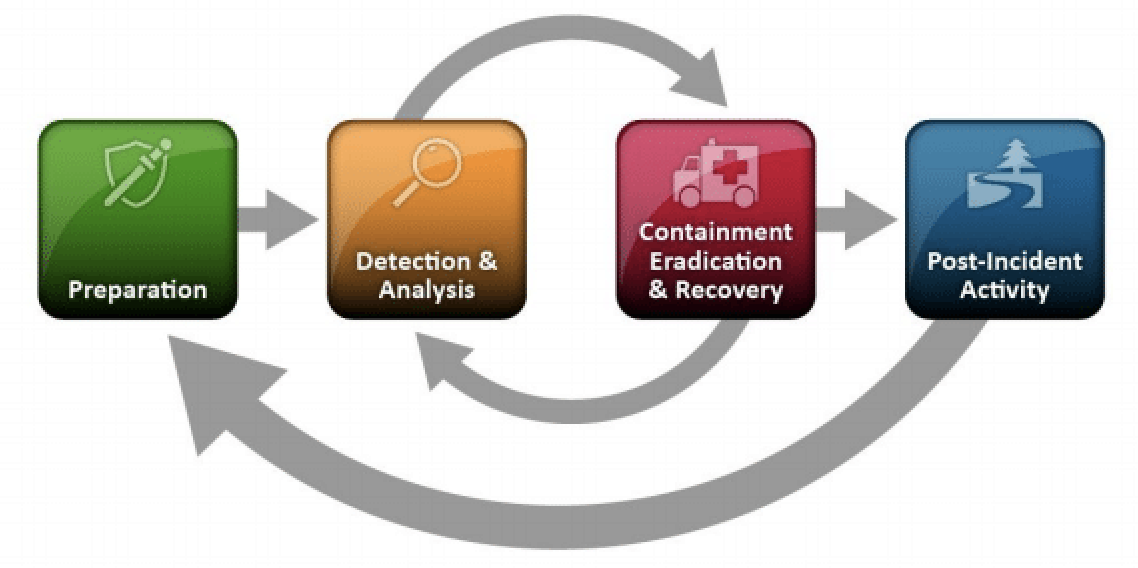
\includegraphics[width=0.8\textwidth]{img/IR.png}
    \caption{Olay Müdahale (Incident Response) Süreci ve Metodolojileri}
    \label{fig:incident-response}
\end{figure}

\begin{figure}[H]
    \centering
    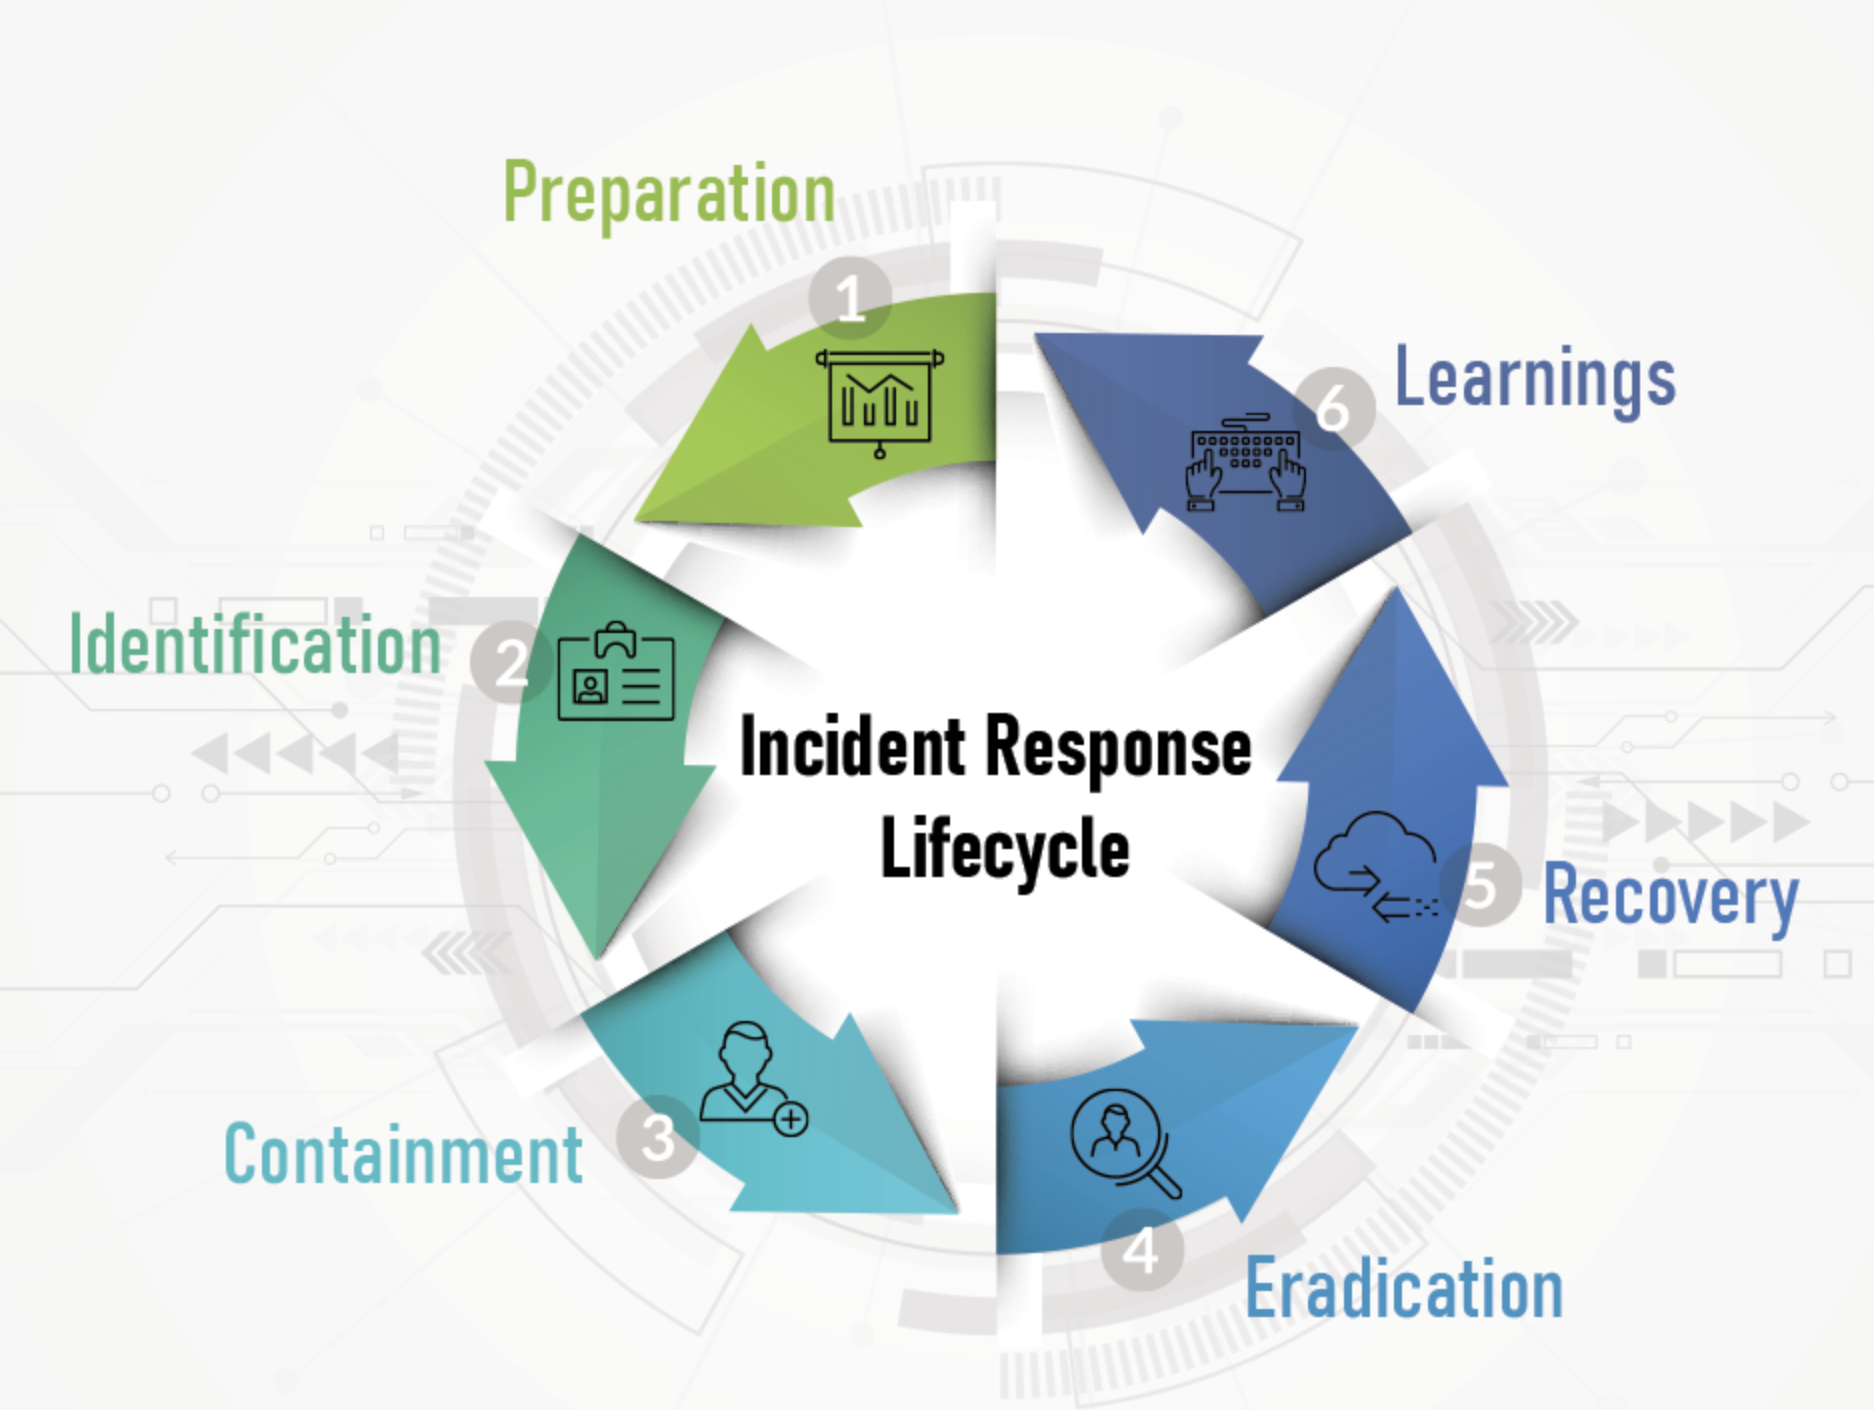
\includegraphics[width=0.8\textwidth]{img/IR_lifecycle.png}
    \caption{Olay Müdahale Yaşam Döngüsü ve Süreç Adımları}
    \label{fig:ir-lifecycle}
\end{figure}



\subsection{Gelişmiş Saldırı Göstergeleri ve Tehdit Avlama}

\subsection{DFIR Metodolojileri: SANS ve NIST Karşılaştırması}

Olay müdahale ve dijital adli bilişim (DFIR) alanında en yaygın kullanılan iki metodoloji, SANS ve NIST'in geliştirdiği çerçevelerdir. Bu metodolojiler, organizasyonların siber olaylara karşı hazırlıklı olmasını ve etkili müdahale etmesini sağlar.

\begin{figure}[H]
    \centering
    
\includegraphics[width=0.7\textwidth]{img/sans-dfir.png}
    \caption{SANS DFIR Metodolojisi ve Süreç Adımları}      
    \label{fig:sans-dfir}
\end{figure}\subsubsection{SANS DFIR Metodolojisi}

SANS, dünya genelinde en çok kullanılan altı adımlı Olay Müdahale (Incident Response) sürecini önerir:

\begin{enumerate}
    \item \textbf{Hazırlık (Preparation):}
    \begin{itemize}
        \item Politika, olay müdahale planı ve araçların oluşturulması
        \item İletişim kanallarının belirlenmesi
        \item Personel eğitimlerinin tamamlanması
    \end{itemize}

    \item \textbf{Tespit (Identification):}
    \begin{itemize}
        \item Olası güvenlik olaylarının belirlenmesi
        \item Uyarılar ve logların analizi
        \item Tehdit istihbaratı ve anomali tespiti
    \end{itemize}

    \item \textbf{Sınırlama (Containment):}
    \begin{itemize}
        \item Kısa vadeli: Etkilenen sistemlerin izolasyonu
        \item Uzun vadeli: Yamalar, güvenlik duvarı kuralları ve ağ segmentasyonu
    \end{itemize}

    \item \textbf{Ortadan Kaldırma (Eradication):}
    \begin{itemize}
        \item Zararlı yazılımın temizlenmesi
        \item Açıklıkların kapatılması
        \item Saldırganın kalıcılığının yok edilmesi
    \end{itemize}

    \item \textbf{Kurtarma (Recovery):}
    \begin{itemize}
        \item Sistemlerin geri yüklenmesi
        \item Bütünlüğün doğrulanması
        \item Normal işleyişe dönüş
    \end{itemize}

    \item \textbf{Dersler (Lessons Learned):}
    \begin{itemize}
        \item Olay sonrası değerlendirme ve raporlama
        \item Kök neden analizi
        \item Savunma mekanizmalarının geliştirilmesi
    \end{itemize}
\end{enumerate}

\subsubsection{NIST DFIR Metodolojisi}

NIST SP 800-61 (Bilgisayar Güvenliği Olay Müdahale Rehberi) dokümanında tanımlanan süreç dört ana aşamadan oluşur:

\begin{enumerate}
    \item \textbf{Hazırlık (Preparation):}
    \begin{itemize}
        \item Politika belirleme ve personel eğitimi
        \item İletişim kanallarının tanımlanması
        \item Tespit araçlarının kurulması
    \end{itemize}

    \item \textbf{Tespit ve Analiz (Detection \& Analysis):}
    \begin{itemize}
        \item Güvenlik uyarıları ve logların izlenmesi
        \item Olayın kapsamı ve türünün belirlenmesi
        \item Ciddiyet sınıflandırması ve önceliklendirme
    \end{itemize}

    \item \textbf{Sınırlama, Ortadan Kaldırma ve Kurtarma:}
    \begin{itemize}
        \item Olayın etkisinin durdurulması
        \item Kök nedenin ortadan kaldırılması
        \item Sistemlerin geri yüklenmesi ve izlenmesi
    \end{itemize}

    \item \textbf{Olay Sonrası Faaliyetler:}
    \begin{itemize}
        \item Alınan derslerin dokümantasyonu
        \item Olay detaylarının belgelenmesi
        \item IR planı ve güvenlik mimarisinin güncellenmesi
    \end{itemize}
\end{enumerate}

\subsubsection{DFIR Metodolojileri}

\begin{table}[ht]
\centering
\begin{tabular}{|l|l|l|}
\hline
\textbf{Kriter} & \textbf{SANS} & \textbf{NIST} \\
\hline
Köken & Eğitim \& sertifikasyon kurumu & ABD federal standart kurumu \\
\hline
Odak & Pratik, uygulayıcı odaklı & Stratejik, politika \& uyumluluk odaklı \\
\hline
DFIR Modeli & 6 adım & 4 adım \\
\hline
Güçlü Yanı & Operasyonel, sahada uygulanabilir & Standartlaştırılmış, politika uyumlu \\
\hline
Kullanım & SOC/IR ekipleri & ABD kamu sektörü \& uyumluluk \\
\hline
\end{tabular}
\caption{DFIR Metodolojileri Karşılaştırması}
\end{table}

Kurumlar genellikle bu iki metodolojinin birleşimini kullanır:
\begin{itemize}
    \item NIST → Politika ve standartlar için
    \item SANS → Operasyonel uygulama için
\end{itemize}

\begin{itemize}
    \item \textbf{Tehdit Avlama Metodolojileri:}
    \begin{itemize}
        \item \textbf{Hipotez Bazlı Avlama:} Örnek: "Sistemde PowerShell Empire kullanıldığına dair göstergeler var mı?"
        \item \textbf{İstihbarat Bazlı Avlama:} Bilinen APT gruplarların TTPs'lerine dayalı arama
        \item \textbf{Anomali Bazlı Avlama:} Normal sistem davranışından sapmaların tespiti
    \end{itemize}

    \item \textbf{Gelişmiş IOC'ler:}
    \begin{itemize}
        \item \textbf{YARA Kuralları:} Zararlı yazılım ailelerini tespit etmek için özel imza tanımları
        \item \textbf{SIGMA Kuralları:} SIEM sistemleri için standartlaştırılmış log analiz kuralları
        \item \textbf{Snort/Suricata Kuralları:} Ağ trafiğinde zararlı aktivite tespiti için kullanılan kurallar
    \end{itemize}

    \item \textbf{Hazırlık (Preparation):} Olayların meydana gelme olasılığını azaltmak için proaktif önlemlerin alındığı aşamadır. Bu aşama, güvenlik açıklarının belirlenmesini ve azaltılmasını, güvenlik politikaları ile prosedürlerinin tanımlanmasını ve bilişim varlıklarının risk analizine göre önceliklendirilmesini içerir. Etkili bir hazırlık için, bir Bilgisayar Güvenlik Olay Müdahale Ekibinin (CSIRT) oluşturulması, iç ve dış paydaşlarla iletişim kanallarının kurulması ve düzenli masa başı (tabletop) tatbikatlarının yapılması hayati önem taşır.

    \item \textbf{Pratik Senaryo - Hazırlık Aşaması Tatbikatı:}
    \begin{itemize}
        \item Bir fidye yazılımı saldırısı için masa başı tatbikatı ele alınabilir. Senaryoda, bir çalışanın e-posta yoluyla fidye yazılımını sisteme bulaştırdığı varsayılır. Olay müdahale ekibi, bu simülasyon sırasında rolleri ve sorumlulukları üzerinden aşağıdaki adımları tartışır:
        \begin{itemize}
            \item Hangi varlıkların (sunucular, veritabanları) öncelikli olarak izole edilmesi gerektiği
            \item İş sürekliliğini sağlamak için hangi alternatif sistemlerin devreye alınacağı
            \item Üst yönetim, hukuk departmanı ve halkla ilişkiler ile hangi iletişim kanallarının kullanılacağı
            \item Verilerin geri yüklenmesi için yedekleme altyapısının test edilmesi ve doğrulanması
        \end{itemize}
    \end{itemize}

\begin{itemize}
    \item \textbf{Tespit ve Analiz (Detection \& Analysis):} Bu aşama, güvenlik olaylarının sürekli izlenmesini ve toplanan verilerin analiz edilmesini içerir. Amaç, şüpheli etkinlikleri gerçek bir siber olaydan ayırt etmektir. Olayın doğası, kapsamı, kökeni ve potansiyel etkisi bu aşamada belirlenir.

    \item \textbf{Sınırlama, Yok Etme ve Kurtarma (Containment, Eradication \& Recovery):} Tespit ve analiz aşamasının ardından, saldırının yayılmasını durdurmak ve zararı en aza indirmek için harekete geçilir. Bu, tehdidin sistemden tamamen temizlenmesini ve iş operasyonlarının normal durumuna geri döndürülmesini kapsar.
\end{itemize}

\subsection{MITRE ATT\&CK Çerçevesi ve Saldırı Tespit Stratejileri}

MITRE ATT\&CK, saldırganların kullandığı taktik ve teknikleri kategorize eden kapsamlı bir bilgi tabanıdır. Bu çerçeve, olay müdahale ve adli bilişim süreçlerinde saldırıların analizi ve savunma stratejilerinin geliştirilmesi için kullanılır.

\begin{itemize}
    \item \textbf{Olay Sonrası Faaliyetler (Post-Incident Activity):} Olay müdahalesinin tamamlanmasından sonra gerçekleştirilen bu aşama, yaşanan olaydan dersler çıkarmayı ve elde edilen bilgileri gelecekteki güvenlik tedbirlerini güçlendirmek için kullanmayı hedefler. Bu süreç, organizasyonun savunma duruşunu sürekli olarak iyileştirme amacını taşır.
\end{itemize}

\subsection{ATT\&CK Matrisi Kullanımı}

\begin{itemize}
    \item \textbf{Taktikler ve Teknikler:}
    \begin{itemize}
        \item \textbf{Başlangıç Erişimi (Initial Access):} Oltalama e-postaları, güvenlik açıklarının istismarı
        \item \textbf{Yetki Yükseltme (Privilege Escalation):} Sistem zafiyetleri, token çalma
        \item \textbf{Yanal Hareket (Lateral Movement):} Pass-the-hash, uzak masaüstü protokolü
        \item \textbf{Veri Hırsızlığı (Exfiltration):} Alternatif protokoller, steganografi
    \end{itemize}

\subsection{Bilgisayar Güvenlik Olay Müdahale Ekibi (CSIRT) Yapısı}

CSIRT, bir organizasyondaki siber güvenlik olaylarını yönetmekle görevli, disiplinler arası ve özel bir ekiptir. Bu ekibin temel amacı, hasarı en aza indirmek ve iş sürekliliğini sağlamaktır. Etkili bir CSIRT operasyonu, sadece teknik uzmanlık değil, aynı zamanda idari ve yasal yetkinlikler de gerektirir.

\begin{itemize}
    \item \textbf{Roller ve Sorumluluklar:} CSIRT, olay yönetimi sürecinin tüm yaşam döngüsünü (hazırlık, tespit, analiz, sınırlama, yok etme, kurtarma ve olay sonrası inceleme) yönetir. Ekip üyeleri, altyapı, işletim sistemleri ve uygulamalar hakkında derinlemesine bilgiye sahip olmalı; etik hacking, bulut güvenliği ve log analizi gibi alanlarda uzmanlık sergilemelidir.

    \item \textbf{Çapraz Fonksiyonel Yapı:} Bir CSIRT, yalnızca teknik uzmanlardan oluşmamalıdır. Hukuk, iletişim, insan kaynakları ve kritik iş birimi yöneticileri gibi farklı departmanlardan temsilcileri içermelidir. Bu çok disiplinli yapı, bir siber saldırının teknik boyutlarının yanı sıra yasal ve itibari sonuçlarının da bütüncül bir yaklaşımla ele alınmasını sağlar. Yönetimden destek ve onay almak, bu ekibin etkin bir şekilde çalışabilmesi için başlangıçta atılması gereken en önemli adımlardan biridir.
\end{itemize}

\subsection{Zararlı Yazılım Analiz Teknikleri}

Modern zararlı yazılımlar, tespit edilmemek için gelişmiş teknikler kullanır. Bu yazılımları analiz etmek için hem statik hem de dinamik analiz teknikleri kullanılır.

\begin{itemize}
    \item \textbf{Statik Analiz:}
    \begin{itemize}
        \item Dosya imzaları ve hash değerleri kontrolü
        \item PE başlık analizi ve bağımlılık incelemesi
        \item Dizi analizi ve şüpheli API çağrılarının tespiti
        \item Yürütülebilir dosya yapısının incelenmesi
    \end{itemize}
\end{itemize}

\subsection{Olay Sınıflandırma, Önceliklendirme ve Ciddiyet Değerlendirmesi}

Olay müdahale sürecinin ilk adımlarından biri, bir olayın ciddiyetini ve potansiyel etkisini değerlendiren "triyaj" sürecidir. Bu aşama, kısıtlı kaynakların en kritik olaylara yönlendirilmesini sağlar ve yanlış pozitif alarmların filtrelenmesine yardımcı olur. Olaylar, saldırı türlerine göre farklı öncelik seviyelerine ayrılır. Örneğin:

\begin{itemize}
    \item \textbf{Keşif ve Araştırma (Probe):} Saldırganın bilgi toplamaya çalıştığı düşük öncelikli olaylar.
    \item \textbf{İstismar ve Kurulum (Exploit \& Installation):} Bir zafiyetin sömürülmesi veya kötü amaçlı yazılımın sisteme yerleştirilmesi girişimi. Bu orta/yüksek öncelikli bir olaydır.
    \item \textbf{Sistemin Ele Geçirilmesi (System Compromise):} Saldırganın sisteme tam erişim sağladığı, en yüksek öncelikli olaydır.
\end{itemize}

\textbf{Pratik Senaryo - Alarm Triyajı:}

Bir SIEM sistemi, aynı IP adresinden 30 saniye içinde 6 başarısız oturum açma girişimi için bir alarm üretir. Bir siber güvenlik analisti bu durumu şu adımlarla yönetir:

\begin{enumerate}
    \item \textbf{Gözden Geçirme:} Analist, alarmı inceler ve benzer olayların geçmişte yaşanıp yaşanmadığını, bu IP adresinin bilinen bir zafiyet tarayıcısına ait olup olmadığını kontrol eder.
    \item \textbf{Sınıflandırma:} Etkinlik, "Brute Force Saldırı Girişimi" olarak sınıflandırılır.
    \item \textbf{Öncelik Belirleme:} Bu bir girişimi temsil ettiği ve henüz sisteme sızma gerçekleşmediği için öncelik seviyesi "Orta" olarak belirlenir.
    \item \textbf{Eskalasyon ve Aksiyon:} Analist, eğer birden fazla IP'den benzer aktiviteler geliyorsa durumu daha ileri analiz için Seviye 2 analiste bildirir ve ilgili IP adresinin güvenlik duvarı üzerinden geçici olarak engellenmesi için bir kural başlatır.
\end{enumerate}

\begin{itemize}
    \item \textbf{Dinamik Analiz:}
    \begin{itemize}
        \item Sanal makine veya sandbox ortamında çalıştırma
        \item Sistem çağrıları ve ağ trafiğinin izlenmesi
        \item Bellek değişikliklerinin analizi
        \item Anti-analiz tekniklerinin tespiti ve bypass edilmesi
    \end{itemize}

    \item \textbf{Davranışsal Analiz:}
    \begin{itemize}
        \item Dosya sistemi aktivitelerinin izlenmesi
        \item Registry değişikliklerinin takibi
        \item Ağ bağlantılarının analizi
        \item Süreç ve servis değişikliklerinin kontrolü
    \end{itemize}
\end{itemize}

\subsection{İletişim Planları ve Paydaş Yönetimi}

Etkin bir olay müdahale planının en önemli bileşenlerinden biri, iç ve dış paydaşlarla nasıl iletişim kurulacağını belirleyen önceden hazırlanmış bir iletişim planıdır. Bu plan, olayın teknik yönlerinin yanı sıra organizasyonun itibarı ve paydaş güveni üzerindeki potansiyel etkilerini yönetmek için tasarlanmıştır.

\begin{itemize}
    \item \textbf{Kritik Paydaşlar:}
    \begin{itemize}
        \item \textbf{İç Paydaşlar:} Üst yönetim, hukuk departmanı, halkla ilişkiler, insan kaynakları ve kritik iş birimi yöneticileri.
        \item \textbf{Dış Paydaşlar:} Yasal ve düzenleyici kurumlar (örneğin Kişisel Verileri Koruma Kurumu), kolluk kuvvetleri, müşteriler, tedarikçiler ve basın.
    \end{itemize}
\end{itemize}

\textbf{Pratik Senaryo - İletişim Akışı:}

Bir veri sızıntısı durumunda iletişim süreci aşağıdaki gibi işleyebilir:

\begin{enumerate}
    \item \textbf{Dahili Bildirim:} CSIRT lideri, veri sızıntısının tespitini hemen üst yönetime ve ilgili iç paydaşlara bildirir. Teknik ekip olayın kapsamını belirlerken, halkla ilişkiler ve hukuk departmanları potansiyel yasal ve kamuoyu yansımaları için hazırlık yapar.
    \item \textbf{Hukuki Bildirim:} Hukuk departmanı, veri sızıntısının yürürlükteki yasalara (ör. KVKK) göre bildirim gerektirip gerektirmediğini değerlendirir. Yasal bildirim süresine uyarak, ilgili düzenleyici kurumlara "derhal" bildirimde bulunulur.
    \item \textbf{Dış Paydaş İletişimi:} İletişim planına uygun olarak, halkla ilişkiler ekibi, durumu net, şeffaf ve abartısız bir dille açıklayan bir basın açıklaması veya müşteri bildirimi hazırlar. Bu açıklama, olayın doğasını, alınan önlemleri ve gelecekteki adımları içerir ve organizasyonun itibarını korumaya yardımcı olur.
\end{enumerate}

\subsection{SOAR (Security Orchestration, Automation and Response)}

SOAR sistemleri, olay müdahale süreçlerini otomatikleştirerek yanıt süresini kısaltır ve insan hatasını azaltır.

\begin{itemize}
    \item \textbf{Otomatik Müdahale Playbook'ları:}
    \begin{itemize}
        \item \textbf{Oltalama E-posta Müdahalesi:}
        \begin{enumerate}
            \item E-postanın otomatik karantinaya alınması
            \item Benzer e-postaların tüm posta kutularında aranması
            \item Şüpheli URL'lerin otomatik engellenmesi
            \item Etkilenen kullanıcıların bilgilendirilmesi
        \end{enumerate}
        \item \textbf{Zararlı Yazılım Müdahalesi:}
        \begin{enumerate}
            \item Etkilenen sistemin otomatik izolasyonu
            \item Zararlı yazılımın karantinaya alınması
            \item Sistem geri yükleme noktası oluşturulması
            \item IOC'lerin SIEM'e otomatik eklenmesi
        \end{enumerate}
    \end{itemize}
\end{itemize}

\begin{itemize}
    \item \textbf{Kolluk Kuvvetleri ile İşbirliği:} Özellikle ciddi siber suçlarda, Türkiye'deki Ulusal Siber Olaylara Müdahale Merkezi (USOM) ve Siber Olaylara Müdahale Ekipleri (SOME) gibi ulusal otoritelerle koordinasyon sağlanması zorunludur.

    \item \textbf{Adli Geçerlilik:} Bir olay sırasında toplanan delillerin mahkemede geçerli sayılması için "gözetim zinciri" (Chain of Custody) olarak bilinen bir prosedürün titizlikle uygulanması gerekir. Bu prosedür, delilin toplanmasından mahkemeye sunulmasına kadar geçen her adımın belgelenmesini, delil bütünlüğünün (hash değerleri ile) korunmasını ve yetkisiz erişime karşı güvenli bir şekilde saklanmasını gerektirir.
\end{itemize}

Olay müdahale süreci, sadece teknik bir problem çözme döngüsü değil, aynı zamanda bütüncül bir kriz yönetimi sürecidir. Bu durum, BT ve güvenlik ekiplerinin, hukuk, iletişim ve üst yönetim gibi diğer departmanlarla sürekli ve entegre bir işbirliği içinde olması gerektiği anlamına gelir. Bu işbirliğinin eksikliği, teknik olarak başarılı bir müdahalenin bile yasal veya itibari bir başarısızlıkla sonuçlanmasına neden olabilir.

\section{Dijital Adli Bilişim Süreçleri}

\subsection{Güvenlik Olayı İzleme ve Alarm Korelasyonu}

Güvenlik Olayı ve Bilgi Yönetimi (SIEM) sistemleri, bir organizasyonun ağındaki çeşitli kaynaklardan gelen günlük (log) verilerini toplayarak şüpheli olayları tespit eder. Alarm korelasyonu, bu sistemlerin sağladığı en önemli işlevlerden biridir. Tek bir olaydan kaynaklanan yüzlerce gereksiz alarmın ("alarm gürültüsü") filtrelenmesini ve bu karmaşanın gerçek tehditlerin gizlenmesine yol açmasının önlenmesini sağlar.

\begin{itemize}
    \item \textbf{API Entegrasyonları:}
    \begin{itemize}
        \item Güvenlik duvarı kurallarının otomatik güncellenmesi
        \item EDR sistemleri ile entegrasyon
        \item Tehdit istihbaratı platformları ile veri alışverişi
        \item İş emri sistemleri ile entegrasyon
    \end{itemize}
    
    \item \textbf{Pratik Korelasyon Kural Örnekleri:}
    \begin{itemize}
        \item \textbf{Brute Force Saldırı Tespiti:} Bir SIEM sistemi, "aynı IP adresinden 30 saniye içinde 6'dan fazla başarısız oturum açma girişimi olursa alarm üret" kuralı ile deneme yanılma saldırılarını otomatik olarak tespit edebilir.
        \item \textbf{Zararlı Yazılım Kontrolü:} "Endpoint koruma sistemi tarafından zararlı olarak tespit edilen bir IP adresi aynı zamanda kritik bir sunucuya oturum başlatırsa alarm üret" kuralı, saldırganın yanal hareketlerini saptamaya yardımcı olur.
        \item \textbf{Log Kaynağı Davranışı Tespiti:} Saldırganlar, tespit edilmekten kaçınmak için log kaynaklarını devre dışı bırakabilirler. Bu duruma karşı "bir uç sistem 1 saatten uzun süre log göndermemişse alarm üret" gibi kurallar yazılabilir.
    \end{itemize}
\end{itemize}

\subsection{Veri Bilimi ve Yapay Zeka Teknikleri}

Modern DFIR süreçleri, büyük veri analizi ve yapay zeka tekniklerinden faydalanır.

\begin{itemize}
    \item \textbf{Makine Öğrenmesi Uygulamaları:}
    \begin{itemize}
        \item \textbf{Anormal Davranış Tespiti:} Kullanıcı davranış analizi (UBA), ağ trafiği anomali tespiti, dosya sistemi aktivite analizi
        \item \textbf{Tehdit İstihbaratı Analizi:} IOC kümeleme ve sınıflandırma, saldırı kampanyası ilişkilendirme, tehdit aktörü profilleme
    \end{itemize}

    \item \textbf{Derin Öğrenme Uygulamaları:} Zararlı yazılım sınıflandırma, şifrelenmiş trafikte anormal davranış tespiti, sıfırıncı gün saldırılarının tespiti
\end{itemize}

\subsection{İlk Müdahale ve Triyaj Prosedürleri}

Olay tespiti yapıldıktan sonraki ilk ve en kritik adım, olayın kapsamını ve önceliğini belirleyen triyaj prosedürleridir. Bu süreç, bir olayın yanlış pozitif mi, yoksa gerçek bir güvenlik ihlali mi olduğunu hızla belirlemeye ve doğru müdahale ekibini atamaya odaklanır.

\begin{itemize}
    \item \textbf{Triyaj Süreci Adımları:}
    \begin{enumerate}
        \item \textbf{Gözden Geçirme:} Seviye 1 analist, SIEM'den gelen alarmı inceler ve bilinen bir güvenlik tarama aracı veya yazılım güncellemesi gibi meşru bir aktivite olup olmadığını kontrol eder.
        \item \textbf{Doğrulama:} Eğer şüphe devam ederse, analist ilgili log kayıtlarını (güvenlik duvarı, uygulama, sistem logları) ve ağ trafiğini inceleyerek olayın gerçek bir saldırı olduğunu doğrular.
        \item \textbf{Sınıflandırma ve Önceliklendirme:} Olay, önceden tanımlanmış kategorilere (ör. oltalama, fidye yazılımı) ve risk matrisine göre (Etki x Ciddiyet) sınıflandırılır ve önceliklendirilir.
        \item \textbf{Eskalasyon:} Olayın ciddiyetine göre, sorumlu yöneticilere ve daha ileri düzeyde teknik yetkinliğe sahip Seviye 2 analistlere bildirimde bulunulur.
    \end{enumerate}
\end{itemize}

\subsection{Delil Toplama ve Gözetim Zinciri Yönetimi}

Dijital delillerin toplanması, adli bilişim sürecinin temelini oluşturur. Bu delillerin, hukuki süreçlerde geçerli sayılabilmesi için değiştirilmediğinden, silinmediğinden ve manipüle edilmediğinden emin olunması gereklidir. Delilin bütünlüğünü korumak için, toplama işlemi sırasında dosyanın "hash" değeri (parmak izi) hesaplanır ve herhangi bir değişiklikte bu değerin değişeceği kabul edilir.

\begin{itemize}
    \item \textbf{Gözetim Zinciri (Chain of Custody):} Bu kavram, delilin olay yerinden toplanmasından mahkemeye sunulmasına kadar geçen süredeki tüm adımların titizlikle belgelenmesini ifade eder. Bu zincir, delilin doğru bir şekilde işlendiğini ve manipüle edilmediğini kanıtlayarak hukuki geçerliliğini sağlar.
\end{itemize}

\textbf{Delil Gözetim Zinciri Formu Örneği}

\begin{longtable}{|>{\tiny}p{0.7cm}|>{\tiny}p{1cm}|>{\tiny}p{0.7cm}|>{\tiny}p{0.7cm}|>{\tiny}p{0.7cm}|>{\tiny}p{0.7cm}|>{\tiny}p{1cm}|}
\caption{Delil Gözetim Zinciri Formu}\\
\hline
\textbf{Delil No.} & \textbf{Delil Tanımı} & \textbf{Tarih/Saat} & \textbf{Yer} & \textbf{Hash (SHA256)} & \textbf{Toplayan} & \textbf{Saklama} \\
\hline
\endfirsthead
\hline
\textbf{Delil No.} & \textbf{Delil Tanımı} & \textbf{Tarih/Saat} & \textbf{Yer} & \textbf{Hash (SHA256)} & \textbf{Toplayan} & \textbf{Saklama} \\
\hline
\endhead
IR-2024-001-H1 & Sunucu 1'in fiziksel disk imajı & 2024-05-15, 10:00 & Sunucu Odası A & \texttt{e4c8e75...} & Ali Kaya & Depo-1, Kilitli Dolap C \\
\hline
IR-2024-001-R1 & Sunucu 1'in RAM dökümü & 2024-05-15, 10:05 & Sunucu Odası A & \texttt{3a5a7d9...} & Veli Yılmaz & Depo-1, Kilitli Dolap C \\
\hline
\end{longtable}
\end{itemize}

\subsection{Kök Neden Analizi ve Saldırı Vektörü Belirleme}

Kök Neden Analizi (RCA), bir siber saldırının yalnızca yüzeysel nedenlerini (ör. bir bilgisayarın enfekte olması) değil, aynı zamanda olayın temelinde yatan asıl nedeni bulmayı amaçlayan sistematik bir çözme yöntemidir. Bu analiz, "neden" sorusunu tekrar tekrar sorarak saldırının nasıl gerçekleştiğini ve hangi zafiyetin sömürüldüğünü detaylıca ortaya çıkarır.

\begin{itemize}
    \item \textbf{Pratik Senaryo - RCA Uygulaması ("5 Neden" Tekniği):}
    \begin{itemize}
        \item \textbf{Sorun:} Kurumun web sitesi, bir siber saldırı sonucu erişilemez hale geldi.
        \item \textbf{1. Neden?} Web sitesi neden erişilemez hale geldi? Çünkü saldırgan SQL enjeksiyonuyla veritabanını sildi.
        \item \textbf{2. Neden?} Saldırgan neden veritabanını silebildi? Çünkü web uygulamasının kullanıcı girdileri düzgün bir şekilde filtrelenmiyordu.
        \item \textbf{3. Neden?} Girdiler neden filtrelenmiyordu? Çünkü geliştirme ekibi bu güvenlik zafiyetini göz ardı eden eski bir kütüphane kullanıyordu.
        \item \textbf{4. Neden?} Bu zafiyet neden göz ardı edildi? Çünkü geliştirme yaşam döngüsüne (SDLC) düzenli güvenlik testleri ve kod incelemeleri entegre edilmemişti.
        \item \textbf{Kök Neden:} Yazılım geliştirme süreçlerinde güvenli kodlama politikalarının ve testlerinin olmamasıdır. Bu analiz, yüzeysel bir teknik sorunun (SQL enjeksiyonu) aslında daha derin bir sistemsel politika eksikliğinden kaynaklandığını göstermektedir.
    \end{itemize}
\end{itemize}

\subsection{Zaman Çizelgesi Oluşturma ve Saldırı Rekonstrüksiyonu}

Olayın her aşamasının kronolojik olarak sıralandığı bir zaman çizelgesi, saldırının nasıl başladığını, nasıl yayıldığını ve hangi sistemleri etkilediğini anlamak için hayati bir araçtır. Adli bilişim uzmanları, sistem, uygulama ve ağ log dosyalarını kullanarak saldırının tüm seyrini yeniden kurgular.

\begin{itemize}
    \item \textbf{Pratik Yönergeler - Zaman Çizelgesi Oluşturma:}
    \begin{enumerate}
        \item \textbf{Veri Toplama:} Etkilenen sistemlerden güvenlik logları (\texttt{security.evtx} - Windows) veya kimlik doğrulama logları (\texttt{/var/log/auth.log} - Linux) toplanır.
        \item \textbf{Normalizasyon:} Farklı formatlardaki loglar, ortak bir formata ve zaman dilimine dönüştürülür.
        \item \textbf{Olay Akışını Kurgulama:} Toplanan olaylar, tarih ve saat bilgisine göre sıralanır. Örnek:
        \begin{itemize}
            \item \texttt{09:30: Yeni kullanıcı (attacker\_user) oluşturuldu.}
            \item \texttt{09:32: attacker\_user RDP ile sisteme bağlandı.}
            \item \texttt{09:35: attacker\_user yetki yükseltme saldırısı gerçekleştirdi.}
        \end{itemize}
    \end{enumerate}
    Bu adımlar, Microsoft Office SmartArt gibi araçlar kullanılarak görsel bir zaman çizelgesine dönüştürülebilir, bu da olay akışının daha kolay anlaşılmasını sağlar. Zaman çizelgesi, adli bilişimin temel amacı olan "ne oldu?" sorusuna yanıt verirken, Kök Neden Analizi "neden oldu?" sorusuna yanıt verir. Bu iki sürecin entegre çalışması, olay müdahale süreçlerinin sadece reaktif değil, aynı zamanda proaktif ve önleyici olmasını sağlar.
\end{itemize}

\section{Uzmanlık Alanları}

\subsection{Kısa Vadeli ve Uzun Vadeli Sınırlama Stratejileri}

Sınırlama, bir siber saldırının yayılmasını durdurarak etkisini en aza indirmeyi amaçlayan en kritik aşamadır. Bu aşama, hem anlık hem de kalıcı önlemleri içerir.

\begin{itemize}
    \item \textbf{Kısa Vadeli Stratejiler:} Saldırı anında uygulanan acil müdahale adımlarıdır.
    \begin{itemize}
        \item Etkilenen sistemlerin ağdan izole edilmesi veya karantinaya alınması.
        \item Saldırganın kullandığı hesapların veya erişim yetkilerinin askıya alınması.
        \item Saldırganın bilinen IP adreslerinin veya alan adlarının güvenlik duvarında engellenmesi.
    \end{itemize}
    \item \textbf{Uzun Vadeli Stratejiler:} Gelecekte benzer saldırıların önlenmesi için kalıcı iyileştirmelerdir.
    \begin{itemize}
        \item Çok Faktörlü Kimlik Doğrulama (MFA) ve geçiş anahtarı (passkeys) gibi güçlü kimlik doğrulama mekanizmalarının uygulanması.
        \item Düzenli güvenlik denetimleri ve sızma testleri gerçekleştirilmesi.
        \item Eski sistem ve yazılımların güncel yamalarla korunması veya değiştirilmesi.
        \item Ağın Sıfır Güven (Zero Trust) prensipleriyle yeniden yapılandırılması.
    \end{itemize}
\end{itemize}

\subsection{Ağ İzolasyonu ve Sistem Karantina Teknikleri}

Ağ izolasyonu, potansiyel tehditlerin yayılmasını önlemek için sistemleri mantıksal veya fiziksel olarak ayırma işlemidir. Bu, olay müdahale süreçlerini kolaylaştırır ve saldırı etkisinin lokalize edilmesini sağlar.

\begin{itemize}
    \item \textbf{İzolasyon Türleri:}
    \begin{itemize}
        \item \textbf{Fiziksel İzolasyon:} Cihazların tamamen ayrı fiziksel ağ altyapılarına bağlanması. Yüksek güvenlik gerektiren ortamlar için kullanılır.
        \item \textbf{Mantıksal İzolasyon:} Aynı fiziksel ağ üzerinde Sanal Yerel Ağlar (VLAN) veya mikrosegmentasyon kullanılarak farklı mantıksal alt gruplar oluşturulur.
    \end{itemize}
\end{itemize}
\textbf{Pratik Yönergeler - Komut Satırı ile İzolasyon:}
\begin{itemize}
    \item \textbf{Windows Ortamı:}
    \begin{itemize}
        \item Bir IP adresinden gelen trafiği engellemek için:
        \begin{verbatim}
netsh advfirewall firewall add rule name="BlokIP" dir=in 
action=block remoteip=192.168.1.10
        \end{verbatim}
        \item Belirli bir programın gelen ve giden tüm bağlantılarını engellemek için:
        \begin{verbatim}
netsh advfirewall firewall add rule name="BlokErisim" dir=in 
action=block program="C:\malware.exe"
        \end{verbatim}
    \end{itemize}
    \item \textbf{Linux Ortamı:}
    \begin{itemize}
        \item Bir IP adresini engellemek için:
        \begin{verbatim}
iptables -A INPUT -s 192.168.1.10 -j DROP
        \end{verbatim}
        \item Belirli bir porta gelen trafiği engellemek için:
        \begin{verbatim}
iptables -A INPUT -p tcp --dport 22 -j DROP
        \end{verbatim}
    \end{itemize}
\end{itemize}
PowerShell betikleri, Azure gibi bulut ortamlarında sanal makineleri (VM) yeni bir alt ağa taşıyarak veya bir ağ güvenlik grubu (NSG) atayarak karantinaya almak için de kullanılabilir.

\subsection{Kötü Amaçlı Yazılım Kaldırma ve Sistem İyileştirme Prosedürleri}

Saldırgan ve kötü amaçlı yazılım kontrol altına alındıktan sonra, sistemden tamamen temizlenmesi gerekir. Bu süreç, otomatik veya manüel yöntemlerle gerçekleştirilebilir.

\begin{itemize}
    \item \textbf{Otomatik Yöntemler:} Microsoft Kötü Amaçlı Yazılımları Temizleme Aracı (MSRT) veya Sophos Scan \& Clean gibi virüs temizleme araçları, yaygın olarak bilinen tehditleri kaldırmak için kullanılır.
    \item \textbf{Manüel Yöntemler:} Daha karmaşık tehditler (rootkit'ler veya gelişmiş kalıcı tehditler) için manüel müdahale gerekebilir.
    \begin{enumerate}
        \item \textbf{Sistem Hizmetlerini Durdurma:} Kötü amaçlı bir hizmetin kalıcı olarak kaldırılması için yönetici komut isteminde \texttt{sc delete "SERVICE NAME"} komutu kullanılır.
        \item \textbf{Kayıt Defteri Temizliği:} Zararlı yazılımlar genellikle sistem başlangıcında çalışmak için kayıt defterine girdi ekler. \texttt{regedit} kullanılarak 
        
        \texttt{HKEY\_CURRENT\_USER\textbackslash{}SOFTWARE\textbackslash{}Microsoft\textbackslash{}}
        
        \texttt{Windows\textbackslash{}CurrentVersion\textbackslash{}Run} 
        
        gibi anahtarlardaki şüpheli girdiler silinir. Bu işlemden önce kayıt defterinin yedeklenmesi kritik öneme sahiptir.
        \item \textbf{Sistem Dosyalarını Onarma:} Zarar görmüş sistem dosyalarını onarmak için \texttt{sfc /scannow} ve \texttt{DISM /Online /Cleanup-Image /RestoreHealth} komutları kullanılır.
    \end{enumerate}
\end{itemize}

\subsection{İş Sürekliliği ve Hizmet Restorasyonu}

Sistemler temizlendikten sonra, iş operasyonlarının normale döndürülmesi sürecine geçilir. Bu süreç, önceden hazırlanmış bir İş Sürekliliği Planı (BCP) ve Felaket Kurtarma (DR) planı ile yönetilir. Felaket Kurtarma, kritik iş uygulamalarının kesintisiz çalışması veya en kısa sürede geri döndürülebilmesi amacıyla tüm sistem ve verilerin farklı bir lokasyonda kopyalanması hizmetidir. Kurtarma sürecinde, verilerin güvenli ve kötü amaçlı yazılımdan arınmış yedeklerden geri yüklendiğinden emin olunmalıdır.

\subsection{Kurtarma Doğrulama ve Güvenlik Duruşu Değerlendirmesi}

Kurtarma işlemi tamamlandıktan sonra, sistemlerin tamamen güvenli olduğunun doğrulanması hayati önem taşır. Bu doğrulama, saldırganın geri dönmesini engelleyecek şekilde güvenlik duruşunun güçlendirildiğini teyit eder. Bu süreç, tüm yamaların ve güncellemelerin uygulandığını, kötü amaçlı yazılım izlerinin kalmadığını ve yeni bir tehdidin ortaya çıkmadığını doğrulamak için uç nokta tespit ve yanıtı (EDR) veya genişletilmiş tespit ve yanıt (XDR) gibi çözümlerle davranışsal analizler yapılmasını içerir.

Olay müdahale döngüsü, sadece geçmişe dönük hasar onarımı değil, aynı zamanda geleceğe dönük bir güvenlik duruşu inşa etmeyi hedefler. Kısa vadeli reaktif adımlar (izolasyon) ile uzun vadeli proaktif stratejiler (yama yönetimi, MFA) arasındaki doğru denge, bir organizasyonun dayanıklılığını belirler.

\section{Olay Sonrası Süreçler}

\subsection{Modern DFIR Araçları ve Platformları}

Dijital Adli Bilişim ve Olay Müdahale (DFIR) süreçlerinde kullanılan çeşitli araçlar, sürecin etkinliğini ve verimliliğini artırır. İşte en önemli DFIR araçları ve özellikleri:

\begin{itemize}
    \item \textbf{Velociraptor:}
    \begin{itemize}
        \item Açık kaynak kodlu uç nokta görünürlük ve toplama aracı
        \item VQL (Velociraptor Query Language) ile güçlü sorgulama yetenekleri
        \item Ölçeklenebilir mimari ve hızlı veri toplama
        \item Özelleştirilebilir "hunt" (av) senaryoları oluşturma imkanı
    \end{itemize}

    \item \textbf{GRR Rapid Response:}
    \begin{itemize}
        \item Google tarafından geliştirilen açık kaynak incident response framework
        \item Python tabanlı uzaktan adli analiz yetenekleri
        \item Büyük ölçekli kurumsal ortamlarda etkili kullanım
        \item Otomatik veri toplama ve analiz iş akışları
    \end{itemize}

    \item \textbf{Autopsy/Sleuth Kit:}
    \begin{itemize}
        \item Açık kaynak dijital adli bilişim platformu
        \item Disk imajı analizi ve dosya kurtarma özellikleri
        \item Timeline analizi ve hash karşılaştırma
        \item Çoklu format desteği (E01, dd, raw vb.)
    \end{itemize}

    \item \textbf{Binalyze IREC:}
    \begin{itemize}
        \item Hızlı forensik veri toplama ve analiz platformu
        \item Tam sistem görünürlüğü ve bellek analizi
        \item Otomatik raporlama ve delil zinciri yönetimi
        \item Cloud entegrasyonu ve uzaktan toplama özellikleri
    \end{itemize}

    \item \textbf{Redline:}
    \begin{itemize}
        \item FireEye tarafından geliştirilen ücretsiz uç nokta analiz aracı
        \item Host-based olay müdahale ve tehdit avcılığı
        \item Bellek ve sistem analizi özellikleri
        \item IOC tarama ve tehdit göstergesi analizi
    \end{itemize}

    \item \textbf{KAPE (Kroll Artifact Parser and Extractor):}
    \begin{itemize}
        \item Hedefli delil toplama ve işleme aracı
        \item Özelleştirilebilir modüller ve hedef profilleri
        \item Hızlı veri toplama ve otomatik işleme
        \item Paralel işleme ve çoklu format desteği
    \end{itemize}

    \item \textbf{THOR (Lite):}
    \begin{itemize}
        \item İleri düzey IOC tarama ve tehdit avcılığı aracı
        \item YARA kuralları ve özel imza desteği
        \item Düşük sistem etkisi ve hızlı tarama
        \item Özelleştirilebilir tarama profilleri
    \end{itemize}
\end{itemize}

\textbf{Araç Seçim Kriterleri:}
\begin{itemize}
    \item \textbf{Kullanım Senaryosu:} Olay türüne ve kapsamına uygun araç seçimi
    \item \textbf{Ölçeklenebilirlik:} Büyük organizasyonlarda etkin kullanım
    \item \textbf{Otomatizasyon:} Tekrarlanan görevlerin otomatikleştirilmesi
    \item \textbf{Entegrasyon:} Mevcut güvenlik altyapısı ile uyum
    \item \textbf{Maliyet:} Açık kaynak vs ticari çözümler değerlendirmesi
\end{itemize}

\subsection{Adli Bilişim Hazırlık ve Planlama}

\begin{figure}[H]
    \centering
    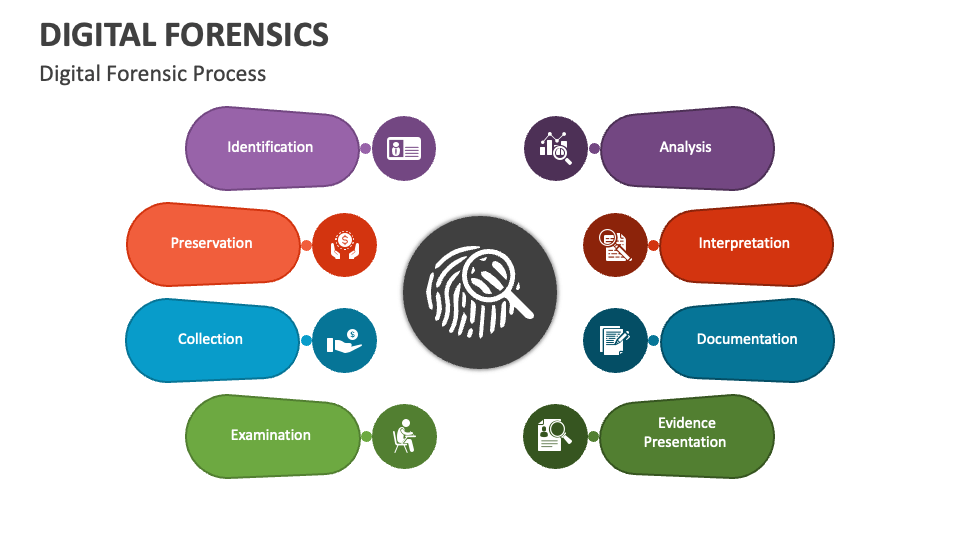
\includegraphics[width=0.9\textwidth]{img/digital-forensics-process.png}
    \caption{Dijital Adli Bilişim Sürecinin Temel Aşamaları ve Metodolojisi}
    \label{fig:digital-forensics-process}
\end{figure}

Adli bilişim, dijital ortamlarda işlenen suçları aydınlatmak için elektronik cihazlardan delil toplama, analiz etme ve hukuki raporlama sürecidir. Bir olay meydana gelmeden önce adli bilişim hazırlığının yapılması, müdahale süresini ve maliyetini azaltır. Bu hazırlık, olay müdahale planına adli bilişim süreçlerinin entegre edilmesini, personelin gerekli eğitimleri almasını ve yazma engelleyiciler, adli bilişim yazılımları (Autopsy, FTK Imager) gibi gerekli araçların hazır bulundurulmasını içerir.

\subsection{Delil Elde Etme: Canlı Sistem ve Post-mortem Analiz}

\begin{itemize}
    \item \textbf{Canlı Sistem Analizi (Live Forensics):} Bir sistem çalışırken, sistem kapandığında kaybolacak olan geçici (volatile) verilerin (bellek içeriği, çalışan süreçler, ağ bağlantıları) toplanmasıdır. Bu veriler, saldırganın sisteme nasıl sızdığına ve ne tür işlemler yaptığına dair kritik ipuçları sağlar.
    \item \textbf{Post-mortem Analiz (Post-mortem Forensics):} Sistem kapalıyken, kalıcı veri depolama birimlerinin (sabit disk, USB bellek) incelenmesidir. Bu işlem, bir delil diskinin bit-bit kopyasının (imajının) alınmasıyla gerçekleştirilir ve bu imaj üzerinde analiz yapılır.
\end{itemize}

\subsection{Bilgisayar Adli Bilişimi: Windows, Linux ve macOS İncelemesi}

Her işletim sisteminin kendine özgü yapısı, adli inceleme yöntemlerini de farklılaştırır.

\begin{itemize}
    \item \textbf{Windows:} Kayıt defteri (Registry) ve merkezi log yönetimi sayesinde analiz daha çok bu verilere odaklanır. Kayıt defteri, kullanıcı aktiviteleri (çalıştırılan programlar, dosya geçmişi) ve sistem yapılandırmaları hakkında zengin bilgi içerir.
    \item \textbf{Pratik Komut Örnekleri (PowerShell):}
    \begin{verbatim}
Get-EventLog -LogName Security -Newest 100
Get-ItemProperty -Path "HKCU:\Software\Microsoft\Windows\
CurrentVersion\Run"
    \end{verbatim}
    \item \textbf{Linux:} Dağıtık günlükleme sistemi ve metin tabanlı yapılandırma dosyaları, daha çok manüel incelemeyi gerektirir.
    \item \textbf{Pratik Komut Örnekleri:}
    \begin{verbatim}
cat /var/log/auth.log | grep "Failed password"
find / -name "backdoor.sh"
    \end{verbatim}
\end{itemize}

\subsection{Ağ Adli Bilişimi ve Trafik Analizi}

Ağ adli bilişimi, bir siber saldırının izini sürmek, saldırı vektörünü belirlemek ve zararlı aktiviteyi ortaya çıkarmak için ağ trafiğini analiz etmeye odaklanır. Trafik, paket yakalama dosyaları (\texttt{.pcap}) halinde kaydedilebilir ve daha sonra incelenebilir.

\begin{itemize}
    \item \textbf{Araçlar:}
    \begin{itemize}
        \item \textbf{Wireshark:} Ağ trafiğini yakalayan, analiz eden ve protokolleri ayrıştıran en yaygın araçlardan biridir.
        \item \textbf{Snort:} Ağ Saldırı Tespit Sistemi (NIDS) olarak çalışarak önceden tanımlanmış kurallara uyan şüpheli paketler için alarm üretir.
    \end{itemize}
\end{itemize}
\textbf{Pratik Senaryo - Wireshark Analizi:}
Bir şüphelinin web sitesine yaptığı kullanıcı adı ve parola girişini incelemek için Wireshark kullanılabilir.
\begin{enumerate}
    \item \textbf{Yakalama:} Wireshark ile ağ arayüzü seçilerek paket yakalama başlatılır.
    \item \textbf{Filtreleme:} Yakalama tamamlandıktan sonra, trafiği daraltmak için \texttt{http.request.method == "POST"} gibi filtreler uygulanır.
    \item \textbf{Paket İncelemesi:} İlgili pakete tıklanarak TCP akışı takip edilir ve bu sayede oturum açma formuna girilen kullanıcı adı ve parola gibi hassas bilgiler incelenir.
\end{enumerate}

\subsection{Mobil Cihaz Adli Bilişimi ve Bulut Adli Bilişimi Zorlukları}

Bu alanlar, adli bilişimin en zorlu alanlarından biridir. Mobil cihazların cihaz çeşitliliği, işletim sistemi farklılıkları ve güçlü şifreleme mekanizmaları, delil elde etmeyi karmaşık hale getirir. Bulut adli bilişimi ise verilerin coğrafi olarak dağıtık olması, yasal yetki alanlarının belirlenmesi ve delilin mülkiyeti gibi sorunları beraberinde getirir.

\begin{itemize}
    \item \textbf{Pratik Yönergeler - Mobil Cihaz Delil Toplama:}
    \begin{enumerate}
        \item \textbf{İzolasyon:} Cihaz, uzaktan silme (remote wipe) veya veri manipülasyonu tehdidine karşı Faraday çantası gibi ekipmanlarla ağdan fiziksel olarak izole edilir.
        \item \textbf{Delil Elde Etme:} Cellebrite UFED veya Oxygen Forensic Detective gibi özel araçlarla cihazın fiziksel veya mantıksal imajı alınır.
    \end{enumerate}
\end{itemize}
Bu alandaki adli bilişim uzmanları, suçluların kullandığı teknolojinin gerisinde kalmamak için sürekli öğrenme ve araç kitlerini güncelleme baskısı altındadır. Mobil ve bulut teknolojilerindeki hızlı gelişmeler, geleneksel adli bilişim metodolojilerinin bu yeni dinamiklere adapte edilmesi gerektiğini göstermektedir.

\section{Uzmanlık Gerektiren Adli Bilişim ve İleri Düzey Analiz}

\subsection{Bellek Adli Bilişimi ve Uçucu Veri Analizi}

Bellek (RAM), bir sistem çalışırken oluşan ve sistem kapatıldığında kaybolan uçucu verileri (işlem parolaları, çalışan süreçler, ağ bağlantıları) içerir. Bu veriler, saldırının kapsamını ve amacını belirlemek için son derece değerli kanıtlar barındırır.

\begin{itemize}
    \item \textbf{Araçlar ve Teknikler:} \textbf{Volatility Framework} gibi bellek analizi araçları, RAM dökümünden bu uçucu verileri çıkarmak için kullanılır.
    \item \textbf{Pratik Yönergeler - Volatility ile Analiz:}
    \begin{enumerate}
        \item \textbf{Bellek Dökümü Alma:} Linux'ta \texttt{dd} komutu veya Windows için geliştirilmiş özel araçlar kullanılarak sistemin belleğinin ham kopyası (dökümü) alınır.
        \item \textbf{Analiz:} Volatility, bu döküm dosyası üzerinde bir dizi komut çalıştırarak analiz yapar:
        \begin{itemize}
            \item \texttt{python3 vol.py -f \textless{}filename\textgreater{} \\ \hspace*{1cm}windows.pslist}: Çalışan tüm süreçleri ve ilişkili PID'lerini listeler. Birçok kötü amaçlı yazılım, gizli süreçler oluşturur ve bunlar bu listelerde tespit edilebilir.
            \item \texttt{python3 vol.py -f \textless{}filename\textgreater{} \\ \hspace*{1cm}windows.netscan}: Bellek dökümü anındaki tüm ağ bağlantılarını, ilişkili süreçleri ve port bilgilerini listeler. Bu komut, bir komuta-kontrol (C2) sunucusuyla olan iletişimi ortaya çıkarabilir.
        \end{itemize}
    \end{enumerate}
\end{itemize}

\subsection{Veritabanı Adli Bilişimi ve Uygulama Log Analizi}

Veritabanları ve uygulamalar, kullanıcı aktiviteleri, hatalar ve kritik işlemler hakkında detaylı kayıtlar (loglar) tutar. Bu loglar, siber saldırıların tespiti, saldırganın hareketlerinin izlenmesi ve adli süreçlerde delil olarak kullanılması açısından hayati öneme sahiptir.

\begin{itemize}
    \item \textbf{Veritabanı Logları (SQL Server Örneği):}
    \begin{itemize}
        \item SQL Server, tüm işlemleri bir işlem günlüğünde (\texttt{.ldf} dosyası) kaydeder.
        \item Adli amaçlar için, \texttt{fn\_dblog()} gibi belgelenmemiş fonksiyonlar, aktif işlem günlüğünü sorgulamaya ve "kimin ne zaman, hangi veriyi değiştirdiği" gibi sorulara yanıt bulmaya olanak tanır.
    \end{itemize}
    \item \textbf{Uygulama Logları:}
    \begin{itemize}
        \item \textbf{Linux Ortamında:} \texttt{grep}, \texttt{awk} ve \texttt{sed} gibi komut satırı araçları, \texttt{syslog} veya \texttt{auth.log} gibi log dosyalarını manüel olarak incelemek için kullanılır.
        \item \textbf{Büyük Ölçekli Sistemlerde:} Logların merkezi olarak toplanması, işlenmesi ve görselleştirilmesi için Elasticsearch, Logstash, Kibana (ELK Stack) gibi kurumsal çözümler kullanılır.
    \end{itemize}
\end{itemize}

\subsection{Endüstriyel Kontrol Sistemi (ICS/SCADA) Adli Bilişimi}

ICS ve SCADA sistemleri, imalat, enerji ve su arıtma gibi kritik endüstriyel süreçleri yöneten sistemlerdir. Bu sistemler, eski teknolojiler, fiziksel etki potansiyeli ve özel ağ protokolleri nedeniyle benzersiz güvenlik ve adli bilişim zorluklarına sahiptir.

\begin{itemize}
    \item \textbf{Adli Bilişim Yaklaşımı:}
    \begin{itemize}
        \item \textbf{Ağ Segmentasyonu:} Saldırının operasyonel teknoloji (OT) ağından bilgi teknolojileri (IT) ağına yayılmasını önlemek için iki ağ fiziksel veya mantıksal olarak ayrılmalıdır.
        \item \textbf{Protokol Analizi:} Modbus, DNP3 gibi endüstriyel protokollere yönelik uzmanlık gerektiren paket analizi yapılır. Bu, saldırganın fiziksel süreçleri manipüle etmeye yönelik komutlarını ortaya çıkarabilir.
        \item \textbf{Sistem Log Analizi:} SCADA master ünitesindeki ve İnsan-Makine Arayüzü (HMI) cihazlarındaki loglar, saldırganın eylemlerini yeniden kurgulamak için incelenir.
    \end{itemize}
\end{itemize}

\subsection{Sanal Makine ve Konteyner Adli Bilişimi}

Sanallaştırma teknolojileri, adli bilişim süreçlerini karmaşıklaştırır.

\begin{itemize}
    \item \textbf{Sanal Makineler (VM):} Bir fiziksel makinenin dijital kopyasıdır ve kendi işletim sistemine sahiptir. VM üzerinde adli bilişim, fiziksel bir makinedekiyle benzer adımlar içerir, ancak analiz sanal disk imajları (\texttt{.vmdk}, \texttt{.vdi}) üzerinde yapılır.
    \item \textbf{Konteynerler (Docker):} İşletim sistemini sanallaştıran ve uygulamayı platformdan bağımsız çalıştıran hafif ortamlardır. Konteynerler geçici ve dinamik olduğu için adli incelemesi zordur. Şüpheli bir konteyner tespit edildiğinde, \texttt{docker commit} komutuyla mevcut durumu yeni bir imaj olarak kaydedilebilir ve bu imaj üzerinde dosya sistemi, bellek ve log analizi yapılabilir.
\end{itemize}

\subsection{Kripto Para ve Blockchain Adli Bilişimi}

Kripto paralar, merkeziyetsiz bir defter teknolojisi olan blockchain üzerinde çalışır. Bu teknoloji, kullanıcıları takma adlar (pseudonymous) kullanarak anonimleştirdiği için finansal suç soruşturmaları için bir zorluk oluşturur. Ancak, blockchain'in değişmez bir kayıt defteri olması, bir kez kaydedilen işlemin manipüle edilememesi anlamına gelir ve bu durum, suçla ilgili kanıtın güvenli bir şekilde saklanmasını sağlar. Adli bilişim uzmanları, kripto para birimlerine ait işlem kayıtlarını takip ederek para akışını izlemeye ve bu akışları gerçek dünya kimlikleriyle ilişkilendirmeye çalışır.

\section{Olay Sonrası Faaliyetler ve Kazanılan Dersler}

\subsection{Olay Dökümantasyonu ve Raporlama Gereksinimleri}

Olay müdahalesinin her aşaması, gelecekteki analizler ve hukuki süreçler için detaylı bir şekilde belgelenmelidir. Olay sonrası rapor (post-mortem), organizasyonun süreç iyileştirmesi için temel bir kaynaktır ve olayın "kim, ne, nerede, ne zaman, neden ve nasıl" sorularına yanıt vermelidir.

\begin{itemize}
    \item \textbf{Olay Sonrası Rapor Şablonu}
    
    \begin{longtable}{|p{3cm}|p{4cm}|p{5.5cm}|}
    \hline
    \textbf{Bölüm} & \textbf{İçerik} & \textbf{Açıklama} \\
    \hline
    \endfirsthead
    \hline
    \textbf{Bölüm} & \textbf{İçerik} & \textbf{Açıklama} \\
    \hline
    \endhead
    \textbf{Yönetici Özeti} & Olayın kısa özeti ve iş üzerindeki etkisi. & Olayın mahiyetine ve sonuçlarına ilişkin üst düzey özet. \\
    \hline
    \textbf{Olay Zaman Çizelgesi} & Olayın kronolojik olarak sıralanmış akışı. & İlk tespitten kurtarmaya kadar her eylemin zaman damgasıyla kaydı. \\
    \hline
    \textbf{Kök Neden Analizi} & Olayın temelinde yatan zafiyetler ve nedenler. & Saldırıya olanak sağlayan sistemsel, teknolojik ve operasyonel açıkların analizi. \\
    \hline
    \textbf{Alınan Aksiyonlar} & Sınırlama, yok etme ve kurtarma aşamalarında yapılanlar. & Hangi sistemlerin izole edildiği, hangi zararlı yazılımların kaldırıldığı, verilerin nasıl geri yüklendiği. \\
    \hline
    \textbf{Kazanılan Dersler ve Öneriler} & Gelecekte benzer olayların önlenmesi için iyileştirme önerileri. & Süreç, politika, teknoloji veya personel farkındalığına yönelik iyileştirme tavsiyeleri. \\
    \hline
    \end{longtable}
\end{itemize}

\subsection{Kazanılan Dersler Analizi ve Süreç İyileştirme}

Olaydan çıkarılan dersler, organizasyonel hafızayı güçlendirir ve aynı hataların tekrarlanmasını önler. Bu süreç, sürekli iyileştirme için bir geri bildirim döngüsü sağlar ve dört temel adımdan oluşur:

\begin{enumerate}
    \item \textbf{Belirleme:} Olaydan elde edilecek önemli kazanımların ve başarıların belirlenmesi.
    \item \textbf{Belgeleme:} Kazanılan derslerin, ilgili herkesin katkıda bulunabileceği bir formatta kaydedilmesi.
    \item \textbf{Analiz Etme:} Elde edilen verilerin incelenerek anlamlı sonuçlar çıkarılması.
    \item \textbf{Saklama:} Raporların, ekiplerin kolayca erişebileceği ortak bir dijital platformda arşivlenmesi.
\end{enumerate}

\subsection{Olaylardan Tehdit İstihbaratı Geliştirme}

Bir siber saldırı, organizasyon için değerli bir tehdit istihbaratı (CTI) kaynağıdır. CTI, ham veriyi (ör. zararlı IP adresleri) işleyerek anlamlı ve eyleme dönüştürülebilir bilgilere dönüştürme sürecidir.

\begin{itemize}
    \item \textbf{İki Önemli Kavram:}
    \begin{itemize}
        \item \textbf{Tehlike Göstergeleri (IOCs):} Kötü amaçlı IP adresleri, dosya hash'leri veya zararlı URL'ler gibi somut, teknik verilerdir. IOC'ler taktiksel düzeyde savunma için kullanılır.
        \item \textbf{Taktik, Teknik ve Prosedürler (TTPs):} Saldırganların amaçlarına ulaşmak için kullandığı yöntemlerdir. TTP'ler, IOC'lere göre daha kalıcıdır ve operasyonel düzeyde savunma için kritik öneme sahiptir.
    \end{itemize}
\end{itemize}
\textbf{İstihbarat Üretimi:}
Bir oltalama saldırısı sonrası tespit edilen zararlı dosya hash'i ve komuta-kontrol sunucusu IP adresi gibi IOC'ler toplanır. Bu veriler, saldırganın kullandığı genel yöntemlerle (ör. belirli bir zararlı yazılım ailesi) ilişkilendirilerek istihbarat haline getirilir ve gelecekteki saldırılara karşı otomatik koruma sağlamak için SIEM ve EDR sistemlerine entegre edilir.

\subsection{Eğitim ve Farkındalık Programı Güncellemeleri}

Bir siber saldırıdan elde edilen dersler, çalışan farkındalık eğitimlerini ve güvenlik prosedürlerini güncellemek için kullanılmalıdır. Olay sonrası yapılan analizler, çalışanların zafiyetli davranışlarını (ör. oltalama e-postalarına tıklama) ortaya çıkarır. Bu geri bildirimler, eğitim materyallerine dahil edilerek simülasyon bazlı testlerle çalışanların farkındalığı artırılır. Siber güvenlik eğitimlerinin de tıpkı diğer eğitim programları gibi, çağın gereklerine göre sürekli revize edilmesi, bu alanda durağanlığın mümkün olmadığının bir göstergesidir.

\subsection{Hukuki Süreç Desteği ve Uzman Tanık İfadeleri}

Siber güvenlik uzmanları, bir adli soruşturma veya mahkeme sürecinde "uzman tanık" olarak görev alabilirler. Hazırladıkları bilimsel mütalaalar, hukuka uygun, somut ve bilimsel verilere dayanmalıdır. Uzman, bulgularını ve vardığı sonuçları mahkemede net, anlaşılır ve basit bir dille açıklamalıdır. Uzmanın sunduğu rapor, hâkimin maddi gerçeği aydınlatmasına ve delilleri doğru yorumlamasına yardımcı olan bir araç olarak kullanılır. Bu durum, teknik uzmanlığın nihayetinde hukuki bir amaca hizmet ettiğini ve uzmanların raporlama ile iletişim becerilerinin de teknik yetkinlikleri kadar kritik olduğunu ortaya koymaktadır.
\chapter{YÖNETİŞİM, RİSK YÖNETİMİ VE UYUMLULUK (GRC)}

\section*{Giriş}

Bu bölüm, bir kuruluşun siber güvenlik duruşunun temel yapıtaşlarını oluşturan, stratejik ve operasyonel GRC (Yönetişim, Risk ve Uyum) mekanizmalarını derinlemesine incelemektedir. Odak noktası, yalnızca teknik kontrollere odaklanmak yerine, güvenliği bir iş önceliği haline getiren ve kuruluşun hedefleriyle hizalayan entegre bir yaklaşım sunmaktır. GRC, organizasyonun güvenli ve doğru yolda kalmasını sağlayan strateji ve yapı olarak işlev görür, bir tripod gibi yönetim, risk yönetimi ve uyumluluk ayaklarını birleştirir.

\section{Uyum Yönetimi ve Düzenleyici Çerçeveler}

\section{Bilgi Güvenliği Yönetişim Çerçevesi}

Bilgi güvenliği yönetişimi, liderlik, organizasyonel yapılar ve süreçlerden oluşan, bilgi varlıklarını korumayı amaçlayan yapılandırılmış bir çerçevedir. Bu çerçeve, güvenliğin "nedenini", "ne olduğunu" ve "kimin sorumlu olduğunu" ele alarak, taktiksel güvenlik tedbirlerinin ötesine geçer ve stratejik bir iş fonksiyonu olarak konumlanmasını sağlar. Bu, yalnızca teknoloji odaklı bir yaklaşımdan ziyade, organizasyonel hedefler ve risk toleransı ile uyumlu güvenlik uygulamalarını garanti eder.

\subsection{Board-level Security Governance ve Oversight (Yönetim Kurulu Seviyesi Siber Güvenlik Gözetimi)}

Yönetim kurulu seviyesinde siber güvenlik gözetimi, siber risklerin kurumsal risk yönetimi (ERM) stratejisinin ayrılmaz bir parçası olarak kabul edilmesini sağlar. Yönetim kurulunun rolü, detaylı teknik operasyonlara müdahale etmekten ziyade, stratejik yönü belirlemek ve kaynakların etkin bir şekilde ayrılmasını sağlamaktır.

Bu katmanda güvenlik, teknik bir konudan stratejik bir iş konusuna dönüşür. Bir siber olayın yol açabileceği itibar kaybı, finansal cezalar ve iş sürekliliği kesintileri gibi doğrudan iş sonuçları, bu risklerin yalnızca teknik değil, aynı zamanda finansal ve operasyonel riskler olarak algılanmasını zorunlu kılar. Bu geniş etki alanı, yönetim kurulunun bütçe onayı, strateji belirleme ve genel gözetim kapsamında bu konuyu aktif olarak ele almasını gerektirir. Bu dönüşüm, güvenlik liderlerinin (örneğin CISO), teknik jargon yerine iş diliyle (risk, yatırım getirisi (ROI), iş etkisi gibi) konuşma becerisine sahip olmasının önemini ortaya koymaktadır. Yönetim kurulu desteği, kaynak tahsisi ve politika onayı için hayati öneme sahiptir.

Yönetim kurulu düzeyinde etkili gözetim mekanizmalarının temel taşları şunlardır:
\begin{itemize}
    \item \textbf{Siber Okuryazarlığın Artırılması:} Yönetim kurulu üyelerinin, genel siber riskler ve şirketi etkileyen özel siber riskler hakkında bilgi edinmesi esastır. Bu, özel eğitimler ve uzmanlarla yapılan görüşmelerle sağlanabilir.
    \item \textbf{Düzenli Raporlama:} Yönetim kurulu, siber güvenlikten sorumlu yöneticilerle düzenli olarak görüşmeli ve şirketin siber olgunluğunu ve dayanıklılığını anlamalarını sağlayan uygun metrikleri talep etmelidir. Bu metrikler, kolayca toplanabilen verilerden ziyade, en riskli alanlara odaklanmalıdır.
    \item \textbf{Görevlerin Ayrılması:} Siber güvenlik stratejisinin belirlenmesi ve bu stratejinin uygulanması arasında görev ayrımının sağlanması kritik öneme sahiptir. Bu, hesap verebilirliği ve etkinliği artırır.
\end{itemize}

\subsection{Information Security Strategy ve Policy Development (Bilgi Güvenliği Stratejisi ve Politika Geliştirme)}

Kapsamlı bir bilgi güvenliği stratejisi ve politikası, sürekli gelişen tehditlere ve karmaşık uyumluluk gereksinimlerine karşı koordineli ve uygulanabilir bir program oluşturur. Bu strateji, organizasyonun tüm güvenlik süreçlerini uçtan uca kapsayan, uygulanabilir ve iş hedeflerine odaklanmış olmalıdır.

Politika geliştirme süreci, tek seferlik bir olaydan ziyade döngüsel bir yapıya sahiptir. Süreç, risk değerlendirmesiyle başlar, ancak politikanın kendisi de risk yönetimi süreçlerinin etkinliğini ölçmek için kullanılır. Bu yaklaşım, güvenlik duruşunun dinamik ve sürekli değişen bir ortamda güncel kalmasını garanti eder.

Bir bilgi güvenliği politikasının adım adım geliştirilmesi için şu adımlar izlenmelidir:
\begin{enumerate}
    \item \textbf{Mevcut Durum ve Risk Değerlendirmesi:} Sürecin ilk adımı, kuruluşun mevcut güvenlik durumunu, hassas verilerini (PII, finansal belgeler vb.), sistemlerini ve potansiyel zayıflıklarını belirleyen kapsamlı bir risk değerlendirmesi yapmaktır. Bu aşama, aynı zamanda organizasyon için kabul edilebilir risk seviyelerini de tanımlar.
    \item \textbf{Yasal ve Sektörel Gereksinimlerin Belirlenmesi:} İlgili tüm yerel, ulusal ve sektörel yasa ve standartlar (KVKK, GDPR, HIPAA, ISO 27001 vb.) incelenir. Bu, politikanın yasal yükümlülüklerle uyumlu olmasını sağlar.
    \item \textbf{Strateji ve Politika Geliştirme:} Değerlendirme sonuçlarına dayanarak, iş hedefleriyle uyumlu bir bilgi güvenliği stratejisi oluşturulur. Bu stratejinin temelini oluşturan yüksek seviyeli ilkeler, ardından detaylı ve konu bazlı politikalara (örneğin, kabul edilebilir kullanım, erişim kontrolü, parola politikası, şifreleme politikası) dönüştürülür. Politika, gizlilik, bütünlük ve erişilebilirlik gibi temel güvenlik hedeflerine odaklanmalıdır.
    \item \textbf{Onay ve İletişim:} Geliştirilen politikalar üst yönetimden onay almalı ve tüm paydaşlara şeffaf bir şekilde iletilmelidir. Politikanın etkinliğini ölçmek için düzenli olarak risk değerlendirmeleri yapılmalı ve bu değerlendirmeler sonucunda belirlenen iyileştirme alanlarına göre politika güncellenmelidir.
\end{enumerate}

\subsection{Security Organization Structure ve Roles/Responsibilities (Güvenlik Organizasyon Yapısı ve Görev/Sorumluluklar)}

Etkili bir yönetişim için net bir organizasyon yapısı ve tanımlanmış roller hayati öneme sahiptir. Siber güvenlik yönetişimi, görev ve sorumlulukların katmanlı bir yapıda olduğunu gösterir.
\begin{itemize}
    \item \textbf{Yönetim Kurulu:} En üst düzeyde stratejik gözetim sağlar ve siber güvenliğin iş hedefleriyle uyumunu denetler. Bu, en üst düzeyde sorumluluk ve hesap verebilirliği tesis eder.
    \item \textbf{Bilgi Güvenliği Komitesi:} Stratejik düzeyde karar alıcı organdır. Kaynak ayrılması, kabul edilebilir risk seviyelerinin belirlenmesi ve risk işleme aksiyonlarının onaylanması gibi görevleri üstlenir. Bu katman, stratejiyi somut eylemlere dönüştüren bağlayıcı noktadır.
    \item \textbf{Bilgi Güvenliği Koordinasyon Ekibi:} Stratejik hedeflerin operasyonel olarak uygulanmasından sorumludur. Risk değerlendirmesi, varlık envanteri oluşturma ve acil durumlarda hasar tespiti gibi çalışmaları yürütür.
    \item \textbf{Bilgi Güvenliği Yöneticisi / Siber Güvenlikten Sorumlu Yetkili Yönetici (SGSYY):} Yönetim sistemi içindeki rol ve sorumlulukları denetler, güvenlik sorunlarına müdahale eder ve gerekli koordinasyonu sağlar.
\end{itemize}

Bu katmanlı yapı, her seviyede şeffaflık ve hesap verebilirlik sağlayarak, güvenliğin tek bir kişiye veya departmana yüklenmesini engeller. Bu, GRC'nin üçayağının (Yönetişim-Risk-Uyum) işlevsel olarak birleştirilmesini de destekler.

\subsection{Security Culture Development ve Awareness Programs (Güvenlik Kültürü Geliştirme ve Farkındalık Programları)}

Güvenlik kültürü, çalışanların güvenliği önceliklendirdiği ve ortak bir sorumluluk olarak gördüğü bir ortamdır. Zira birçok güvenlik ihlali, oltalama saldırıları veya kullanıcı hatalarından kaynaklanır.

Güvenlik kültürü oluşturmak, sadece eğitimlerle sınırlı kalmamalı, sürekli ve katılımcı bir süreç olmalıdır. Bu süreç, üst yönetimin desteğiyle başlar; yönetim kademesi, güvenlik standartlarını belirleyerek ve güvenliği teşvik ederek örnek olmalıdır. Ardından, çalışanlara düzenli olarak siber güvenlik eğitimleri verilmelidir. Bu eğitimler, kimlik avı saldırılarını tespit etme, parola yönetimi, fiziksel güvenlik ve çıkarılabilir medya kullanımı gibi konuları içermelidir.

Pratik uygulamalar ve simülasyonlar, teorik bilgilerin pekiştirilmesi için kritik öneme sahiptir. Oltalama (phishing) simülasyonları gibi pratik testler, çalışanların riskli davranışlarını değerlendirmek ve güvenli alışkanlıklar geliştirmelerine yardımcı olmak için kullanılmalıdır.

\textbf{Adım Adım Oltalama (Phishing) Simülasyonu Yürütme Kılavuzu:}
\begin{enumerate}
    \item \textbf{Hedef Kitleyi Belirleyin:} Simülasyonun hangi çalışan gruplarını veya departmanlarını hedefleyeceğini netleştirin.
    \item \textbf{Senaryo Oluşturun:} Mevcut şablonlardan veya sıfırdan bir senaryo seçin. Senaryolar genellikle gerçek dünyadaki oltalama tekniklerini taklit eder. Popüler senaryo örnekleri şunlardır:
    \begin{itemize}
        \item \textbf{CEO Dolandırıcılığı:} Üst düzey bir yöneticinin acil para transferi talep ettiği bir e-posta, duygusal ve hiyerarşik bir tetikleyici kullanır.
        \item \textbf{Sahte Şifre Sıfırlama:} LinkedIn gibi güvenilir bir platformdan geldiği iddia edilen, acil şifre sıfırlama uyarısı içeren bir e-posta, aciliyet hissi yaratır.
        \item \textbf{İnsan Kaynakları Politikası Güncellemesi:} Çalışanlara iç ve rutin görünen, yeni bir sağlık hizmeti planı veya ödeme politikası hakkında bilgi veren bir e-posta.
    \end{itemize}
    \item \textbf{Simülasyonu Yapılandırın:} Oltalama e-postasının içeriğini ve yönlendireceği sahte web sayfasını hazırlayın. Bu aşamada, sahte bir giriş sayfası veya zararlı bir dosya indirme bağlantısı içeren bir "yük" (payload) yapılandırılır.
    \item \textbf{Kampanyayı Başlatın:} Simülasyonu başlatma ve bitiş tarihlerini belirleyin. Hedef kitleye otomatik olarak e-postalar gönderilecektir.
    \item \textbf{Sonuçları İzleyin ve Raporlayın:} Kampanya sonuçları (tıklama oranları, veri girişi, raporlama sayısı) izlenerek, riskli kullanıcılar ve güvenlik açıkları belirlenir.
    \item \textbf{Eğitim Ataması:} Başarısız olan çalışanlara otomatik olarak düzeltici eğitimler atanır. Bu, sadece bir test değil, aynı zamanda sürekli bir öğrenme sürecidir.
\end{enumerate}

\subsection{Third-party Risk Governance ve Vendor Management (Üçüncü Taraf Risk Yönetimi ve Tedarikçi Yönetimi)}

Üçüncü taraflara (tedarikçiler, iş ortakları, bulut servis sağlayıcıları) olan bağımlılık arttıkça, bu tarafların yarattığı riskleri yönetmek hayati hale gelmektedir. Kaynaklar, tek bir tedarikçiye aşırı bağımlılığın (single-source) maliyeti optimize edebilse de, operasyonel zafiyetler yarattığını ve iş sürekliliğini tehdit ettiğini belirtmektedir. Uzun süreli ve başarılı vendor ilişkileri, risklerin ortadan kalktığına dair yanlış bir güven duygusu yaratabilir. Bu durum, izleme ve acil durum planlaması çabalarını azaltmaya yol açabilir. Coğrafi olarak aynı bölgede bulunan birden fazla tedarikçi de, doğal afetler gibi lokal olayların tedarik zincirini aynı anda kesintiye uğratmasına neden olabilir.

Bu riskleri yönetmek için kapsamlı bir Üçüncü Taraf Risk Yönetimi (TPRM) programı kurulmalıdır:
\begin{enumerate}
    \item \textbf{Kapsam ve Envanter:} Tedarik zinciri haritasını çıkararak tüm tedarikçileri, hizmet sağlayıcıları ve yüklenicileri kapsamlı bir şekilde listelemekle başlanır.
    \item \textbf{Riske Dayalı Değerlendirme:} Tüm üçüncü taraflara aynı risk değerlendirme süreci uygulanmamalıdır. Bunun yerine, riske orantılı bir yaklaşım benimsenerek, hassas verilere erişenler gibi kritik tedarikçilere daha derinlemesine incelemeler yapılmalıdır.
    \item \textbf{Durum Tespiti (Due Diligence):} Yeni bir tedarikçi ile çalışmaya başlamadan önce, siber güvenlik duruşu, finansal istikrar ve uyumluluk geçmişi gibi konularda kapsamlı bir durum tespiti yapılmalıdır. Bu, kabul edilemez risk seviyelerine sahip tedarikçilerle çalışmaktan kaçınmayı sağlar.
    \item \textbf{Sözleşmeler ve SLA'lar:} Tedarikçilerle imzalanan sözleşmeler ve hizmet seviyesi anlaşmaları (SLA), beklentileri açıkça belirlemeli ve olası kesintilere karşı bir koruma sağlamalıdır.
    \item \textbf{Sürekli İzleme ve Denetim:} Tedarikçi risk profillerindeki değişiklikler düzenli olarak değerlendirilmeli ve gerektiğinde denetimler yapılmalıdır. Bu, risklerin dinamik doğasına uyum sağlamak için esastır.
\end{enumerate}

\section{Kurumsal Risk Yönetimi ve Siber Risk}

Risk yönetimi, işletmenin hedeflerine ulaşmasını engelleyebilecek olumsuz sonuçlara yol açabilecek her şeyi yönetme sürecidir. Bu süreç, belirsizliği ortadan kaldırmayı ve uyumluluk gerekliliklerini karşılamayı amaçlar.

\subsection{ISO 31000 Risk Management Framework (ISO 31000 Risk Yönetim Çerçevesi)}

\textbf{NIST Risk Yönetim Çerçevesi (RMF)}, altı aşamalı bir risk yaşam döngüsü sunar: Kategorize Et, Seç, Uygula, Değerlendir, Yetkilendir ve İzle. Bu sistematik yaklaşım, organizasyonların siber güvenlik risklerini kapsamlı bir şekilde yönetmesini sağlar.

ISO 31000:2018, bir yönetim sistemi standardı olmamasına rağmen, organizasyonların riskleri tanımlaması, analiz etmesi ve yönetmesi için sistematik bir rehber sunar. Bu çerçeve, kuruluşların risk bilincini artırarak karar alma süreçlerini destekler ve sürdürülebilir başarıyı teşvik eder.

Standardın temel ilkeleri şunları içerir:
\begin{itemize}
    \item \textbf{Entegre Yaklaşım:} Risk yönetimi, tüm iş süreçlerine ve karar alma mekanizmalarına entegre edilmelidir.
    \item \textbf{Özelleştirilmiş ve Esnek Olmak:} Çerçeve, her organizasyonun kendine özgü ihtiyaçlarına göre uyarlanabilmelidir.
    \item \textbf{İnsan ve Kültür Faktörleri:} İnsanların algıları ve kültürel faktörler risk yönetiminin başarısını doğrudan etkiler.
    \item \textbf{Sürekli İyileştirme:} Risk yönetimi dinamik bir süreçtir ve sürekli öğrenme ile geliştirilmelidir.
\end{itemize}

\subsection{FAIR (Factor Analysis of Information Risk) Risk Analiz Metodolojisi}

FAIR, bilgi riskini nicel olarak ölçmek için tasarlanmış sistematik bir metodoloji ve uluslararası standart (ISO/IEC 27005 eki) olarak kabul edilmiştir. Geleneksel risk değerlendirmelerinde sıkça karşılaşılan "yüksek-orta-düşük" gibi subjektif değerlendirmelerin yerine, finansal etkiyi sayısal olarak hesaplayabilen bir yaklaşım sunar.

\textbf{FAIR Temel Modeli:}

FAIR, riski iki ana bileşen olarak tanımlar:
\begin{enumerate}
    \item \textbf{Kayıp Olayı Frekansı (Loss Event Frequency - LEF):} Belirli bir tehdidin belirli bir sürede ne sıklıkla gerçekleşebileceğini tahmin eder.
    \item \textbf{Kayıp Büyüklüğü (Loss Magnitude - LM):} Bir kayıp olayının gerçekleşmesi durumunda ortaya çıkacak finansal etkinin miktarını hesaplar.
\end{enumerate}

Risk = LEF × LM formülü ile hesaplanır.

\textbf{FAIR Detaylı Risk Faktörleri:}

\begin{longtable}{|p{3cm}|p{4cm}|p{6cm}|}
\caption{FAIR Risk Faktörleri ve Hesaplama Yöntemleri}\\
\hline
\rowcolor{tableheadcolor}
\textbf{Ana Faktör} & \textbf{Alt Faktörler} & \textbf{Açıklama ve Hesaplama} \\
\hline
\endfirsthead
\multicolumn{3}{c}{\small\tablename\ \thetable\ -- devamı} \\
\hline
\rowcolor{tableheadcolor}
\textbf{Ana Faktör} & \textbf{Alt Faktörler} & \textbf{Açıklama ve Hesaplama} \\
\hline
\endhead
\hline
\multicolumn{3}{r}{\small Devamı sonraki sayfada} \\
\endfoot
\hline
\endlastfoot
Tehdit Olayı Frekansı & Tehdit Kapasitesi, Kontrol Gücü & Bir tehdit aktörünün saldırı gerçekleştirme yeteneği ve mevcut kontrollerin etkisiz hale getirilme ihtimali \\
\hline
Zafiyet & Kontrol Gücü, Tehdit Kapasitesi & Mevcut güvenlik kontrollerinin zayıflıkları ve tehdit aktörünün bunları istismar etme yeteneği \\
\hline
Birincil Kayıp & Veri Kaybı, Sistem Kaybı & Doğrudan maddi kayıplar: veri kurtarma, sistem yenileme, operasyonel kesinti maliyetleri \\
\hline
İkincil Kayıp & İtibar Kaybı, Yasal Cezalar & Dolaylı etkiler: müşteri kaybı, düzenleyici cezalar, hisse değeri düşüşü \\
\hline
\end{longtable}

\textbf{FAIR Uygulama Adımları:}

\begin{enumerate}
    \item \textbf{Kapsam Tanımlama:} Analiz edilecek varlık, tehdit ve senaryo netleştirilir
    \item \textbf{Veri Toplama:} Geçmiş olaylar, endüstri verileri ve uzman görüşleri toplanır
    \item \textbf{Kalibrasyon:} Belirsizlik aralıkları ve olasılık dağılımları belirlenir
    \item \textbf{Monte Carlo Simülasyonu:} Binlerce senaryo çalıştırılarak risk dağılımı hesaplanır
    \item \textbf{Sonuç Analizi:} 95\% güven aralığı ve beklenen yıllık kayıp (ALE) raporlanır
\end{enumerate}

\subsection{Compliance Framework'leri ve Düzenleyici Gereksinimler}

Modern organizasyonlar, faaliyet gösterdikleri sektörlere ve coğrafi konumlara bağlı olarak çoklu düzenleyici gereksinimleri karşılamak zorundadır. Bu compliance landscape'i karmaşık ve sürekli değişen bir yapı arz etmektedir.

\textbf{Temel Compliance Çerçeveleri:}

\begin{longtable}{|p{2.5cm}|p{3cm}|p{4cm}|p{3cm}|}
\caption{Majör Compliance Framework'leri Karşılaştırması}\\
\hline
\rowcolor{tableheadcolor}
\textbf{Framework} & \textbf{Kapsam} & \textbf{Temel Gereksinimler} & \textbf{Hedef Sektör} \\
\hline
\endfirsthead
\multicolumn{4}{c}{\small\tablename\ \thetable\ -- devamı} \\
\hline
\rowcolor{tableheadcolor}
\textbf{Framework} & \textbf{Kapsam} & \textbf{Temel Gereksinimler} & \textbf{Hedef Sektör} \\
\hline
\endhead
\hline
\multicolumn{4}{r}{\small Devamı sonraki sayfada} \\
\endfoot
\hline
\endlastfoot
ISO 27001 & Bilgi güvenliği yönetim sistemi & 114 kontrol, risk yönetimi, sürekli iyileştirme & Tüm sektörler \\
\hline
SOX & Finansal raporlama & IT kontrolleri, veri bütünlüğü, erişim kontrolleri & Halka açık şirketler (ABD) \\
\hline
GDPR & Kişisel veri koruma & Veri minimizasyonu, izin yönetimi, ihlal bildirimi & AB verileri işleyen tüm org. \\
\hline
KVKK & Kişisel veri koruma & Veri işleme kayıtları, DPO atama, etki analizi & Türkiye'deki organizasyonlar \\
\hline
HIPAA & Sağlık verisi koruma & Şifreleme, erişim kontrolü, denetim kayıtları & ABD sağlık sektörü \\
\hline
PCI DSS & Ödeme kartı verisi & Ağ segmentasyonu, şifreleme, penetrasyon testleri & Ödeme işleyen kuruluşlar \\
\hline
NIST CSF & Siber güvenlik çerçevesi & Belirle, koru, tespit et, müdahale et, kurtar & Kritik altyapılar \\
\hline
\end{longtable}

\textbf{Compliance Program Yönetimi:}

Etkili bir compliance programı, sadece düzenleyici gereksinimleri karşılamakla sınırlı kalmamalı, aynı zamanda organizasyonun risk duruşunu güçlendiren stratejik bir avantaj sağlamalıdır.

\begin{enumerate}
    \item \textbf{Gap Analizi ve Başlangıç Değerlendirmesi:} Mevcut kontroller ile gereksinimler arasındaki boşlukların belirlenmesi
    \item \textbf{Compliance Roadmap Geliştirme:} Önceliklendirme, zaman çizelgeleri ve kaynak planlaması
    \item \textbf{Politika ve Prosedür Geliştirme:} Düzenleyici gereksinimleri operasyonel süreçlere çevirme
    \item \textbf{Kontrolların İmplementasyonu:} Teknik ve idari kontrollerin sistematik uygulanması
    \item \textbf{Sürekli İzleme ve Denetim:} Compliance durumunun düzenli değerlendirilmesi
    \item \textbf{Olay Müdahale ve Raporlama:} Düzenleyici bildirimleri ve düzeltici eylemler
\end{enumerate}

\textbf{Automated Compliance Management:}

Modern compliance yönetimi, otomasyon araçları olmadan sürdürülebilir değildir. GRC platformları şu yetenekleri sağlar:

\begin{itemize}
    \item \textbf{Kontrol Mapping:} Çoklu framework'lerdeki benzer kontrollerin eşleştirilmesi
    \item \textbf{Evidence Collection:} Denetim kanıtlarının otomatik toplanması ve arşivlenmesi
    \item \textbf{Risk Assessment Integration:} Compliance durumunun risk skorlaması ile entegrasyonu
    \item \textbf{Dashboard ve Raporlama:} Yönetim için gerçek zamanlı compliance metrikleri
    \item \textbf{Workflow Automation:} Düzeltici eylem planlarının takibi ve eskalasyonu
\end{itemize}

\subsection{Cyber Risk Quantification ve Business Impact Analysis (Siber Riskin Nicelleştirilmesi ve İş Etki Analizi)}

Siber riskin nicelleştirilmesi, riskleri soyut terimler ("yüksek/orta/düşük") yerine somut finansal değerlerle ifade etmeyi amaçlayan bir yaklaşımdır. Bu, karar alma süreçlerini daha objektif hale getirir ve güvenlik yatırımlarının iş üzerindeki etkisini net bir şekilde gösterir.

\textbf{İş Etki Analizi (BIA) Adım Adım Yönergesi:}
BIA, bir siber olayın kritik iş operasyonları üzerindeki potansiyel etkilerini sistematik olarak değerlendiren bir süreçtir. BIA'nın çıktıları, Felaket Kurtarma Planı (DRP) için gerekli olan Kurtarma Süresi Hedefi (RTO) ve Kurtarma Noktası Hedefi (RPO) gibi hedeflerin belirlenmesinde temel veri kaynağını oluşturur. Bir BIA, kritik iş süreçlerinin ne kadar süre durabileceğini ve ne kadar veri kaybına dayanabileceğini değerlendirerek, teknik ekiplerin Felaket Kurtarma Planı (DRP) için net RTO ve RPO değerleri belirlemesini sağlar.

BIA'nın temel adımları şunlardır:
\begin{enumerate}
    \item \textbf{Kapsamı Tanımlayın:} Hangi iş birimlerinin, süreçlerinin ve sistemlerinin analize dahil edileceğini netleştirin.
    \item \textbf{Kritik İş Fonksiyonlarını Belirleyin:} Kuruluşun temel operasyonlarını ve hizmetlerini listeleyin. Her bir fonksiyon için potansiyel finansal, operasyonel ve itibar kayıplarını belirleyin.
    \item \textbf{Bağımlılıkları Haritalandırın:} Kritik fonksiyonların hangi IT sistemlerine, verilere, personele ve üçüncü taraf hizmetlerine bağımlı olduğunu çıkarın.
    \item \textbf{Etkileri Değerlendirin:} Her bir kesintinin zaman içindeki (örneğin, ilk birkaç saat, ilk 24 saat, ilk hafta) potansiyel etkilerini (gelir kaybı, yasal cezalar, itibar zedelenmesi) finansal olarak ölçün.
\end{enumerate}

\subsection{FAIR (Factor Analysis of Information Risk) Methodology (FAIR Metodolojisi)}

FAIR, siber riskleri parasal terimlerle nicelleştiren ve subjektif ("yüksek/orta/düşük") değerlendirmelerden objektif, veriye dayalı analize geçişi sağlayan uluslararası bir standarttır. Bu model, güvenlik yatırımlarının işe yaradığını göstermek ve bütçe kararlarını desteklemek için stratejik bir dilde iletişim kurmaya olanak tanır.

\begin{figure}[H]
    \centering
    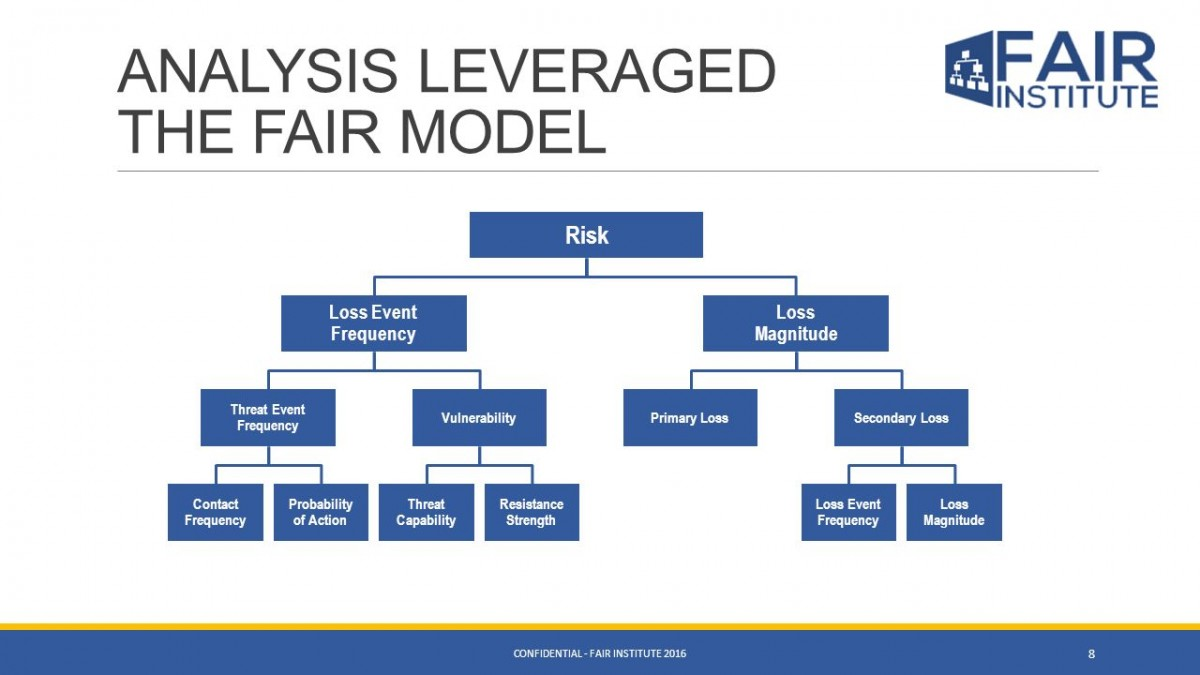
\includegraphics[width=0.8\textwidth]{img/FAIR-Cyber-Risk-Quantification-model.png}
    \caption{FAIR Siber Risk Nicelleştirme Modeli}
    \label{fig:fair-risk-model}
\end{figure}

FAIR metodolojisi, riski iki ana bileşene ayırır:
\begin{itemize}
    \item \textbf{Kayıp Olayı Frekansı (Loss Event Frequency - LEF):} Belirli bir süre zarfında bir kayıp olayının ne sıklıkta meydana gelme olasılığını ölçer.
    \item \textbf{Kayıp Büyüklüğü (Loss Magnitude - LM):} Bir kayıp olayının potansiyel etkisini finansal olarak ifade eder. Bu, birincil (üretkenlik kaybı, müdahale maliyeti) ve ikincil (itibar kaybı, yasal cezalar) kayıpları içerir.
\end{itemize}

\textbf{Pratik FAIR Analiz Senaryosu: Bir Çalışanın Dizüstü Bilgisayarının Çalınması}

\begin{itemize}
    \item \textbf{Senaryo:} "Ayrıcalıklı bir çalışanın, hassas müşteri verilerini içeren dizüstü bilgisayarının çalınmasıyla ilişkili riski analiz edin".
    \item \textbf{Adım 1: Değerleme (Varlık Değeri):} Varlığın değeri sadece fiziksel cihaz değil, asıl olarak içerdiği hassas veridir (PII, entelektüel mülkiyet, vb.).
    \item \textbf{Adım 2: Tek Kayıp Beklentisi (Single Loss Expectancy - SLE) Hesaplaması:} Bu, tek bir olaydan kaynaklanan maliyettir.
    \begin{itemize}
        \item \textbf{Formül:} SLE = Varlık Değeri $\times$ Maruz Kalma Faktörü
        \item \textbf{Örnek Uygulama:}
        \begin{itemize}
            \item Varlık Değeri: \$2.500 (laptop) + \$22.500 (hassas PII verisi, önceki olaylara göre belirlenen yasal maliyetler, itibar kaybı vb.) = \textbf{\$25.000}.
            \item Maruz Kalma Faktörü: Şifrelenmemiş veriye sahip bir laptop çalındığında bu \%100'dür.
            \item SLE: \$25.000 $\times$ \%100 = \$25.000
        \end{itemize}
    \end{itemize}
    \item \textbf{Adım 3: Yıllık Meydana Gelme Oranı (Annual Rate of Occurrence - ARO) Hesaplaması:} Bu, yılda kaç kez bu tür bir olayın meydana gelmesinin beklendiğidir.
    \begin{itemize}
        \item \textbf{Örnek Uygulama:} Geçmiş olaylara bakılarak, yılda ortalama 11 laptop hırsızlığı yaşanmışsa, ARO değeri \textbf{11}'dir.
    \end{itemize}
    \item \textbf{Adım 4: Yıllık Kayıp Beklentisi (Annual Loss Expectancy - ALE) Hesaplaması:} Bu, bir riskten kaynaklanan yıllık maliyet beklentisidir.
    \begin{itemize}
        \item \textbf{Formül:} ALE = SLE $\times$ ARO
        \item \textbf{Örnek Uygulama:} \$25.000 $\times$ 11 = \$275.000
    \end{itemize}
\end{itemize}

Aşağıdaki tablo, bu FAIR analiz senaryosunu özetlemektedir:

\begin{center}
\begin{tabularx}{0.95\textwidth}{|>{\raggedright\arraybackslash}X|>{\raggedright\arraybackslash}X|>{\centering\arraybackslash}X|}
\hline
\textbf{Bileşen} & \textbf{Tanım} & \textbf{Değer} \\
\hline
\textbf{Varlık} & Çalınan dizüstü bilgisayarın değeri, içerdiği hassas PII verisi dahil & 25.000\$ \\
\hline
\textbf{Tek Kayıp Beklentisi (SLE)} & Tek bir olayın maliyeti (\$25.000 $\times$ \%100 maruz kalma faktörü) & 25.000\$ \\
\hline
\textbf{Yıllık Meydana Gelme Oranı (ARO)} & Yılda beklenen olay sayısı & 11 \\
\hline
\textbf{Yıllık Kayıp Beklentisi (ALE)} & Yıllık toplam beklenen maliyet (\$25.000 $\times$ 11) & 275.000\$ \\
\hline
\end{tabularx}
\end{center}

Bu tür nicel veriler, soyut bir tehdidi finansal terimlere dökerek, güvenlik yöneticilerinin üst yönetimle aynı dilde konuşmasını sağlar ve bütçe gerekçelendirmesini kolaylaştırır.

\subsection{Risk Appetite ve Tolerance Definition (Risk İştahı ve Tolerans Tanımı)}

Risk iştahı, organizasyonun hedeflerini takip ederken kabul etmeye istekli olduğu genel risk seviyesidir. Risk toleransı ise, belirli bir risk türü için kabul edilebilir varyasyonun daha granüler bir yansımasıdır. Risk toleransı, risk iştahı doğrultusunda, belirli sınırlar ve eşikler belirler.

\subsection{Risk Treatment Strategies ve Control Selection (Risk Ele Alma Stratejileri ve Kontrol Seçimi)}

Risk değerlendirmesi tamamlandıktan sonra, kuruluşlar riskleri yönetmek için stratejiler belirler. Başlıca stratejiler şunlardır:
\begin{itemize}
    \item \textbf{Kaçınma (Avoidance):} Riski tamamen ortadan kaldırmak için ilgili aktiviteyi veya sistemi terk etme. Örneğin, hassas verileri güvensiz bir bulut hizmetinde depolamaktan kaçınmak.
    \item \textbf{Azaltma (Loss Prevention and Reduction):} Kontroller uygulayarak bir olayın oluşma sıklığını veya etkisini azaltma. Bu, en yaygın siber güvenlik stratejisidir. Örneğin, güvenlik duvarları ve şifreleme kullanmak.
    \item \textbf{Transfer Etme (Transfer):} Riski finansal olarak başka bir tarafa devretme. En yaygın örneği siber sigorta almaktır. Bu, riskin finansal yükünü sigorta şirketine aktarır.
    \item \textbf{Kabul Etme (Retention):} Riski bilerek ve isteyerek kabul etme ve sonuçlarına katlanma kararı. Bu, riski yönetmenin maliyetinin, riskin gerçekleşme olasılığı veya etkisinden daha yüksek olduğu durumlarda tercih edilebilir.
\end{itemize}

\subsection{OCTAVE FORTE Risk Değerlendirme Metodolojisi}



OCTAVE FORTE (Operationally Critical Threat, Asset, and Vulnerability Evaluation), Carnegie Mellon Üniversitesi tarafından geliştirilen sistematik bir bilgi güvenliği risk değerlendirme metodolojisidir. Bu çerçeve, organizasyonların kritik varlıklarını belirlemelerine, tehditleri değerlendirmelerine ve risk azaltma stratejileri geliştirmelerine yardımcı olur.

\section{Uyum Yönetimi ve Düzenleyici Çerçeveler}

Uyum (compliance), bir organizasyonun yasalara, düzenlemelere ve standartlara uyma eylemidir. Yönetişim içsel hedeflerle ilgiliyken, uyumluluk dışsal gereksinimlere odaklanır.

\subsection{Regulatory Compliance Assessment ve Gap Analysis (Düzenleyici Uyum Değerlendirmesi ve Açık Analizi)}

Açık analizi (gap analysis), bir kuruluşun mevcut politika, prosedür ve uygulamalarını belirli bir düzenleyici çerçeveye (örneğin, GDPR, HIPAA) göre değerlendirerek eksiklikleri belirleme sürecidir.

\textbf{Adım Adım Gap Analizi:}
\begin{enumerate}
    \item \textbf{Kapsamı Tanımlayın:} Hangi düzenlemelere ve standartlara uyum sağlanması gerektiğini net bir şekilde belirleyin.
    \item \textbf{Mevcut Durumu Gözden Geçirin:} Mevcut politikaları, kontrolleri ve prosedürleri kapsamlı bir şekilde inceleyin. Bu, belgeleme, uygulamalar ve teknolojileri içerir.
    \item \textbf{Açıkları Belirleyin:} Mevcut durum ile uyum gereklilikleri arasındaki tutarsızlıkları listeleyin. Bu, eksik kontrolleri, güncel olmayan politikaları veya eksik belgeleri içerebilir.
    \item \textbf{Açıkları Önceliklendirin:} Her açığı, potansiyel etkisi ve risk seviyesine göre sıralayın. Örneğin, müşteri verilerinin şifrelenmemesi, ağır finansal cezalara ve itibar kaybına yol açabileceği için yüksek öncelikli bir açık olabilir.
\end{enumerate}

\subsection{Internal Audit Programs ve Control Testing (Kurum İçi Denetim Programları ve Kontrol Testi)}

Kurum içi denetim programları, siber güvenlik süreçlerinin, politikalarının ve araçlarının etkinliğini değerlendirmek ve potansiyel tehditlere karşı uygun kontrollerin mevcut olduğunu doğrulamak için kritik öneme sahiptir. Bu denetimler, riskleri belirlemeye ve gidermeye yardımcı olurken, aynı zamanda dış denetimlere hazırlık sağlar.

\subsection{External Audit Coordination ve Remediation Management (Dış Denetim Koordinasyonu ve İyileştirme Yönetimi)}

Dış denetimler, üçüncü bir tarafın uyumluluğu doğrulaması için yapılır. Başarılı bir dış denetim, titiz bir hazırlık ve denetim bulgularının etkin bir şekilde giderilmesini gerektirir. Uyum otomasyon araçları, denetim sürecini kolaylaştırarak kanıt toplama ve raporlama yükünü azaltır.

\subsection{Compliance Automation Tools ve Continuous Monitoring (Uyum Otomasyon Araçları ve Sürekli İzleme)}

Sürekli uyum, kuruluşun uyumluluk gerekliliklerini yıl boyunca sürekli olarak izlemesini ve uyumsuzluk sorunlarını ortaya çıktıkça gerçek zamanlı olarak gidermesini sağlayan bir süreçtir. Bu, uyumu tek bir yıllık denetim etkinliğinden sürekli bir sürece dönüştürür.

Bu otomasyon, geleneksel manuel süreçlerin zaman alıcı ve kaynak yoğun doğasını ortadan kaldırır. Otomasyon araçları (SIEM, SOAR), kanıt toplama ve kontrol testini otomatikleştirerek insan müdahalesini \%80 oranında azaltabilir. Bu, kuruluşların denetime hazır olma süresini haftalara indirebilir ve proaktif bir duruşa geçişi temsil eder.

\textbf{Sürekli İzleme İçin Temel Araçlar:}
\begin{itemize}
    \item \textbf{Güvenlik Bilgileri ve Olay Yönetimi (SIEM):} SIEM araçları (Splunk, IBM QRadar, SolarWinds Security Event Manager) çeşitli kaynaklardan (sunucular, uygulamalar, ağ cihazları) gelen logları ve olay verilerini toplar, normalleştirir ve ilişkilendirir. Bu, gerçek zamanlı olarak tehditleri ve güvenlik ihlallerini tespit etmeyi sağlar. Örneğin, bir sağlık kuruluşu, HIPAA uyumluluğunu sağlamak için bir SIEM kullanır. SIEM, elektronik sağlık kayıtlarına yetkisiz erişimi izler ve raporlar oluşturur.
    \item \textbf{Siber Güvenlik Orkestrasyonu, Otomasyonu ve Müdahalesi (SOAR):} SOAR platformları, SIEM'den gelen uyarıları alır ve önceden tanımlanmış "playbook"lar (oyun planları) aracılığıyla otomatik veya yarı otomatik müdahale eylemleri başlatır.
\end{itemize}

\textbf{Örnek SOAR Playbook (Oltalama Saldırısı Müdahalesi):}
\begin{enumerate}
    \item \textbf{Algılama:} SIEM, bir e-posta güvenliği ağ geçidinden şüpheli bir e-posta uyarısı alır.
    \item \textbf{Sınıflandırma ve Analiz:} SOAR, e-postadaki göstergeleri (URL, IP, dosya hash'leri) otomatik olarak çıkarır ve üçüncü taraf tehdit istihbaratı araçlarıyla karşılaştırır. Bu analiz, e-postanın kötü amaçlı olup olmadığını doğrular.
    \item \textbf{İçerme (Containment):} Eğer e-posta kötü amaçlı olarak doğrulanırsa, SOAR tüm kullanıcıların gelen kutularındaki şüpheli e-postaları otomatik olarak karantinaya alır ve ilgili etki alanlarını güvenlik duvarı seviyesinde engeller.
    \item \textbf{Kaldırma (Eradication):} Analiz tamamlandıktan sonra, SOAR tehdidin etkisiz hale getirildiğini doğrular ve ilgili güvenlik olayını kapatır.
\end{enumerate}

\subsection{Cross-border Compliance ve Data Sovereignty (Sınır Ötesi Uyum ve Veri Egemenliği)}

Veri egemenliği, dijital verilerin üretildiği ülkenin yasalarına ve yönetişim yapılarına tabi olduğu ilkesidir. Bu durum, özellikle çok uluslu şirketler için sınır ötesi veri transferlerini karmaşık bir hale getirir.

\textbf{Yeterlilik Kararları (Adequacy Decisions):} Avrupa Komisyonu tarafından verilen bir yeterlilik kararı, AB dışındaki bir ülkenin kişisel veriler için yeterli düzeyde koruma sağladığını resmen onaylar. Bir ülke "yeterlilik" statüsü kazandığında, kişisel veriler AB'den bu ülkeye ek koruyucu önlemler (örneğin, Standart Sözleşme Maddeleri - SCC'ler) olmaksızın serbestçe akabilir. Bu, veri transfer süreçlerini teknik ve operasyonel olarak basitleştirir.

Yeterlilik kararı olmadığında, kuruluşlar veri transferlerini sağlamak için "uygun güvenceler" (appropriate safeguards) kullanmak zorundadır. Bu güvenceler şunları içerir:
\begin{itemize}
    \item \textbf{Standart Sözleşme Maddeleri (SCC'ler):} Bunlar, veri koruma yetkilileri tarafından onaylanmış ve veri transferinde kullanılması gereken yasal metinlerdir. Bu maddeler, transferin teknik olarak nasıl gerçekleştirileceğini (şifreleme, erişim kontrolü vb.) dolaylı olarak etkileyebilir.
    \item \textbf{Bağlayıcı Şirket Kuralları (BCR'ler):} Çok uluslu şirketler için geçerli olan, dahili veri transferlerini yöneten, denetim makamları tarafından onaylanması gereken bağlayıcı kurallardır.
\end{itemize}

Bu durum, gizlilik mühendisliği kontrollerinin (örneğin, şifreleme) yalnızca iyi bir uygulama değil, aynı zamanda belirli yasal durumlarda zorunlu bir gereklilik haline geldiğini göstermektedir.

\section{Güvenlik Metrikleri, KPIs ve Performans Ölçümü}

Güvenlik metrikleri ve temel performans göstergeleri (KPI'lar), bir siber güvenlik programının etkinliğini ölçmek, tehdit eğilimlerini anlamak ve yatırım kararlarını gerekçelendirmek için kullanılır. Bu veriler, güvenlik durumunun tarihsel bir perspektifini sunarak, zaman içindeki eğilimleri ve değişiklikleri görmeyi sağlar.

\subsection{Security Performance Indicator Development (Güvenlik Performans Göstergesi Geliştirme)}

Güvenlik metrikleri, yatırımları izlemenin ötesine geçerek tehdit modelleri, olay müdahale verimliliği ve sistem zafiyetleri hakkında içgörüler sunar. Bu göstergeler, güvenlik stratejilerinin ne kadar etkili olduğunu anlamak için kritik öneme sahiptir.
\begin{itemize}
    \item \textbf{KPI Örnekleri:}
    \begin{itemize}
        \item Algılama Süresi (Mean Time to Detect - MTTD) ve Müdahale Süresi (Mean Time to Respond - MTTR).
        \item Yamalı ve güncel cihazların yüzdesi.
        \item Siber güvenlik farkındalık eğitimi tamamlama oranı.
        \item Saldırı girişimlerinin sayısı.
    \end{itemize}
\end{itemize}

\subsection{Risk Metrics ve Trend Analysis (Risk Metrikleri ve Trend Analizi)}

Risk metrikleri, riskin parasal terimlerle nicelleştirilmesine olanak tanır ve zaman içindeki eğilimleri analiz etmeye yardımcı olur. Bir statik sayıdan ziyade, zaman içindeki ilerlemeyi gösteren bir trend çizgisi, üst yönetim için daha anlamlıdır.
\begin{itemize}
    \item \textbf{Kullanım Alanları:}
    \begin{itemize}
        \item \textbf{Nicel Risk Değerleri:} FAIR metodolojisinden elde edilen Yıllık Kayıp Beklentisi (ALE) gibi metrikler, riski objektif olarak değerlendirmeyi sağlar.
        \item \textbf{Trend Analizi:} Güvenlik olaylarının sayısı veya bir riskin parasal değeri, düzenli aralıklarla izlenerek bir trend grafiği oluşturulabilir.
    \end{itemize}
\end{itemize}

\subsection{Executive Dashboard Design ve Reporting (Yönetici Kontrol Paneli Tasarımı ve Raporlama)}

Yöneticilere yönelik bir kontrol paneli, kapsamlı ve teknik verilerde kaybolmadan yüksek seviyeli risk, uyumluluk ve stratejik hedeflere doğru ilerleme hakkında genel bir bakış sunar.

\textbf{Tasarım İlkeleri:}
\begin{enumerate}
    \item \textbf{Hedef Kitleyi Tanıyın:} Yönetim kurulu üyeleri stratejik kararlar alırlar, bu nedenle raporlar finansal etki, risk azaltma ve iş değeri gibi konulara odaklanmalıdır.
    \item \textbf{Sadelik:} Dashboard, beş ila altı temel "kart" veya bileşenle sınırlı olmalı ve trafik ışığı protokolü (kırmızı, sarı, yeşil) gibi basit görsel ipuçları kullanmalıdır.
    \item \textbf{Hikaye Anlatma:} Statik veriler yerine, zaman içindeki ilerlemeyi gösteren trend çizgileri kullanılmalıdır. Bu, güvenlik yatırımlarının işe yaradığını gösteren bir hikaye anlatmaya yardımcı olur.
\end{enumerate}

\textbf{Örnek Dashboard Metrikleri:}
\begin{itemize}
    \item Genel Risk Skoru (Nicel bir değer)
    \item Politikalara Uyum Seviyesi (Yüksek, Orta, Düşük)
    \item MTTD ve MTTR Trendleri
    \item Saldırı Girişimleri Sayısı ve Kaynağı
\end{itemize}

\subsection{Security Investment ROI Calculation (Güvenlik Yatırımı ROI Hesaplaması)}

Güvenlik yatırımlarının geri dönüşünü (ROSI), geleneksel finansal ROI formüllerinin ötesinde, azaltılan potansiyel kayıplar üzerinden hesaplamak gerekir.

\begin{equation}
ROSI = \frac{(ALE \times \text{Azaltma Oranı}) - \text{Çözüm Maliyeti}}{\text{Çözüm Maliyeti}}
\end{equation}

\textbf{Örnek Senaryo:}
\begin{itemize}
    \item \textbf{Senaryo:} Fidye yazılımı ve DDoS saldırılarına karşı bir Yönetilen Güvenlik Hizmeti Sağlayıcısı (MSSP) çözümü almayı değerlendiren bir kuruluş.
    \item \textbf{Veriler:} Fidye yazılımı ve DDoS için beklenen toplam yıllık kayıp beklentisi (ALE) 41.500.000\$. Çözümün bu tehditleri önlemedeki etkinliği (azaltma oranı) \%80 ve yıllık maliyeti 120.000\$.
    \item \textbf{Hesaplama:}
    \begin{equation*}
    ROSI = \frac{(41,500,000 \times 0.8) - 120,000}{120,000} = 275.67 = 27,567\%
    \end{equation*}
\end{itemize}

Güvenlik yatırımları doğrudan gelir getirmediği için finans ekipleri için değeri genellikle belirsizdir. ROSI formülü, bu soyut yararı (azaltılan risk) somut, parasal bir değere dönüştürür. Yapılan hesaplama, her bir dolarlık güvenlik yatırımının 275 dolar potansiyel kaybı önlediğini gösterir. Bu nicel veri, yöneticilerin bütçe kararlarını gerekçelendirmesine yardımcı olur.

\subsection{Benchmark Analysis ve Peer Comparison (Kıyaslama Analizi ve Akran Karşılaştırması)}

Kıyaslama analizi, bir organizasyonun güvenlik duruşunu sektördeki veya benzer büyüklükteki akranlarına göre değerlendirme sürecidir. Bu, kuruluşun kendi performans hedeflerini belirlemesine ve yatırım yapılacak alanlara odaklanmasına yardımcı olur. Etkin kıyaslama için, yüksek kaliteli veri, ortak bir terminoloji ve karşılaştırılabilir metriklerin kullanımı esastır.

\section{İş Sürekliliği ve Felaket Kurtarma Planlaması}

İş sürekliliği planlaması (BCP), bir kriz anında temel iş süreçlerinin devamlılığını sağlamayı amaçlayan geniş kapsamlı bir yaklaşımdır. Felaket Kurtarma Planı (DRP) ise, BCP'nin teknolojiye odaklanan, veri kurtarma ve IT sistemlerini yeniden çalışır hale getirme üzerine yoğunlaşan bir alt kümesidir.

\subsection{Business Impact Analysis (BIA) ve Criticality Assessment (İş Etki Analizi ve Kritiklik Değerlendirmesi)}

BIA, bir olayın en önemli iş süreçlerini nasıl etkileyeceğini anlamak için kritik bir ilk adımdır. Bu analiz, varlıkların önceliklendirilmesine temel oluşturur ve kaynakların en kritik alanlara ayrılmasını sağlar. Adımlar, bir varlık envanteri oluşturmayı, varlıkları iş fonksiyonlarına göre kritikliklerine göre sıralamayı ve potansiyel etkilerini değerlendirmeyi içerir.

\subsection{Recovery Time Objective (RTO) ve Recovery Point Objective (RPO) (Kurtarma Süresi ve Kurtarma Noktası Hedefi)}

Bu hedefler, bir felaket durumunda kurtarmanın nasıl önceliklendirileceğini ve ne kadar hızlı gerçekleşeceğini belirler.
\begin{itemize}
    \item \textbf{RTO (Recovery Time Objective):} Bir uygulamanın, işi olumsuz etkilemeye başlamadan önce maksimum kapalı kalabileceği süredir.
    \item \textbf{RPO (Recovery Point Objective):} Bir kesinti anında kabul edilebilir maksimum veri kaybı miktarıdır. Bu, veri yedekleme sıklığını belirler.
\end{itemize}

Aşağıdaki tablo, farklı iş süreçleri için RTO ve RPO hedeflerini kritiklik seviyelerine göre sınıflandırmaktadır:

\begin{center}
\begin{longtable}{|>{\raggedright\arraybackslash}p{3cm}|>{\raggedright\arraybackslash}p{3cm}|>{\centering\arraybackslash}p{2.5cm}|>{\centering\arraybackslash}p{2.5cm}|}
\caption{İş Kritikliği Seviyelerine Göre RTO ve RPO Hedefleri} \\
\hline
\textbf{İş Kritikliği Seviyesi} & \textbf{Örnek İş Süreci} & \textbf{RTO (Kurtarma Süresi)} & \textbf{RPO (Kurtarma Noktası)} \\
\hline
\endfirsthead
\multicolumn{4}{l}{\small\tablename\ \thetable\ -- devamı} \\
\hline
\textbf{İş Kritikliği Seviyesi} & \textbf{Örnek İş Süreci} & \textbf{RTO (Kurtarma Süresi)} & \textbf{RPO (Kurtarma Noktası)} \\
\hline
\endhead
\hline
\multicolumn{4}{r}{\small Devamı sonraki sayfada} \\
\endfoot
\hline
\endlastfoot
\textbf{Görev-Kritik (Mission-Critical)} & Müşteri Sipariş Sistemi, Finansal İşlemler & Saniyelerden Dakikalara & 0-15 dakika \\
\hline
\textbf{Temel (Essential)} & E-posta, İK Uygulamaları & 4 ila 24 saat & 1-24 saat \\
\hline
\textbf{Kritik Olmayan (Nonessential)} & İç Raporlama Araçları, İdari Dosyalama & 24 saatten Haftalara & 24 saatten haftalara \\
\end{longtable}
\end{center}

Bu matris, IT ve iş ekiplerinin kurtarma öncelikleri üzerinde ortak bir anlayışa sahip olmasını sağlar, böylece kaynaklar en acil ihtiyaçlara yönlendirilebilir.

\subsection{Disaster Recovery Planning ve Testing (Felaket Kurtarma Planlaması ve Testi)}

DRP, siber saldırı, doğal afet veya sistem arızası gibi olaylara müdahale etmek için stratejiler ve protokoller sağlayan bir yol haritasıdır. Bir DRP'nin var olması yeterli değildir; planın gerçek bir kriz anında işe yaradığından emin olmak için düzenli olarak test edilmesi ve güncellenmesi gerekir.

\textbf{Plan Oluşturma Adımları:}
\begin{enumerate}
    \item \textbf{Ekip Kurma:} Kriz anında müdahale çabalarına liderlik edecek bir afet müdahale ekibi oluşturun.
    \item \textbf{Altyapı Planı:} Ağ altyapınızın ve sistem bağımlılıklarının detaylı bir planını çizin.
    \item \textbf{Kurtarma Prosedürlerini Belgeleyin:} Hasarlı sistemleri, uygulamaları ve verileri kurtarmak için adım adım talimatları basit bir dille yazın. Bu plan ağdan uzak bir yerde veya değişmez (immutable) depolama alanında saklanmalıdır.
\end{enumerate}

\textbf{Test ve Tatbikat Türleri:}
\begin{itemize}
    \item \textbf{Masaüstü Tatbikatları (Tabletop Exercises):} Ekip, bir senaryoyu (örneğin, fidye yazılımı saldırısı) sözlü olarak tartışır, rolleri ve prosedürleri gözden geçirir.
    \item \textbf{Simülasyonlar:} Gerçek bir kesintiyi simüle ederek, sistemlerin kurtarma kabiliyetini test eder. Bu testler, planın zayıf yönlerini ortaya çıkarır ve bu eksiklikler, gerçek bir olaydan önce giderilebilir.
\end{itemize}

\subsection{Crisis Management ve Emergency Response (Kriz Yönetimi ve Acil Durum Müdahale)}

Bir siber saldırı, özellikle fidye yazılımı (ransomware), özel bir müdahale planı gerektirir. Aktörlerin sizi izleyebileceği düşünülerek, müdahale işlemleri koordineli bir şekilde ve bant dışı (out-of-band) iletişim kanalları (telefon görüşmeleri) kullanılarak yapılmalıdır.

\textbf{Fidye Yazılımı Müdahale ve Kurtarma Planı (Teknik Playbook):}
\begin{enumerate}
    \item \textbf{İçerme (Containment):} Ağdaki enfekte sistemleri hemen belirleyin ve yalıtın.
    \begin{itemize}
        \item \textbf{Teknik Adımlar:} Etkilenen sistemlerin ağ kablosunu çekin veya kablosuz bağlantısını kesin. Enfeksiyonun yayılmasını engellemek için anahtar (switch) seviyesinde ağı kapatmak en etkili yöntem olabilir.
    \end{itemize}
    \item \textbf{Delil Toplama:} Forensik inceleme için etkilenen sistemlerin imajını alın ve uçucu hafıza içeriğini (volatile memory) yakalayın.
    \item \textbf{Temizleme (Eradication):} Tüm enfekte sistemleri silin veya dezenfekte edin.
    \item \textbf{Kurtarma ve Yeniden İnşa:} Yedeklerden geri yüklemeye başlayın.
\end{enumerate}

\begin{verbatim}
--Veritabanı Geri Yükleme (SQL Server Örneği):
RESTORE DATABASE [veritabani_adi] \
    FROM DISK = '[yedek_dosyasi_yolu]' \
    WITH RECOVERY
\end{verbatim}

\begin{verbatim}
--Anlık Görüntü (Snapshot) Geri Yükleme (AWS RDS Örneği):
aws rds restore-db-cluster-from-snapshot \
    --db-cluster-identifier my-db-cluster \
    --snapshot-identifier my-snapshot-id \
    --engine aurora-postgresql
\end{verbatim}

\begin{verbatim}
--Dosya Geri Yükleme (Linux Örneği):
restore -xvqf /dev/rmt0 /home/mike/tools
\end{verbatim}

\subsection{Supply Chain Continuity ve Vendor Dependency Management (Tedarik Zinciri Sürekliliği ve Tedarikçi Bağımlılık Yönetimi)}

İşletmelerin giderek daha karmaşık hale gelen tedarik zincirlerine bağımlı olması, bu zincirdeki kesintilere karşı dayanıklılık oluşturmayı zorunlu hale getirir. Bu dayanıklılığı artırmak için şu stratejiler benimsenmelidir:
\begin{itemize}
    \item \textbf{Proaktif Tanımlama:} Kritik vendor bağımlılıklarını önceden belirleyin ve tek kaynaklı tedarik anlaşmalarının potansiyel tehlikelerini anlayın.
    \item \textbf{Alternatif Kaynak Geliştirme:} Kriz anında hızlı geçişi mümkün kılmak için önceden nitelikli, alternatif tedarikçilerle ilişkiler kurun.
    \item \textbf{SLA ve Sözleşme Güçlendirme:} Kesinti anında tedarikçi sorumluluklarını netleştiren güçlü sözleşmeler hazırlayın.
\end{itemize}

\section{Gizlilik Yönetimi ve Veri Koruma Yönetişimi}

Gizlilik yönetimi, özellikle kişisel verilerin korunmasına odaklanan GRC'nin kritik bir bileşenidir.

\subsection{Privacy by Design ve Privacy Impact Assessments (Tasarım Yoluyla Gizlilik ve Gizlilik Etki Değerlendirmeleri)}

Tasarım yoluyla gizlilik (Privacy by Design), gizliliği bir sistemin veya projenin başlangıç tasarımından itibaren entegre etme ilkesidir. Gizlilik Etki Değerlendirmesi (PIA), bu ilkenin pratik bir uygulamasıdır. PIA, özellikle kişisel verilerin işlenmesi yüksek risk taşıyorsa veya yeni teknolojiler kullanılıyorsa zorunludur.

\subsection{Data Protection Officer (DPO) Role ve Responsibilities (Veri Koruma Görevlisi Rolü ve Sorumlulukları)}

Veri Koruma Görevlisi (DPO), kuruluşun veri koruma kurallarına uyumunu sağlamaktan sorumlu kilit bir pozisyondur.
\begin{itemize}
    \item \textbf{Temel Sorumlulukları:} Yönetime ve çalışanlara veri koruma yükümlülükleri hakkında danışmanlık yapmak, uyumluluğu izlemek ve veri sahiplerinden gelen talepler için iletişim noktası olmak.
    \item \textbf{DPO'nun Konumu:} DPO, görevlerini bağımsız bir şekilde yerine getirebilmeli ve yönetim çatışmasından kaçınmak için diğer görevlerle çelişmemelidir.
\end{itemize}

\subsection{Data Subject Rights Management ve Breach Notification (Veri Sahibi Hakları Yönetimi ve İhlal Bildirimi)}

Veri sahipleri, kişisel verileri üzerinde belirli haklara sahiptir. Kuruluşlar, bu hakları yönetmek için süreçler kurmalıdır. Kişisel veri ihlali durumunda, kontrolör, mümkünse ihlalin farkına vardıktan sonra en geç 72 saat içinde yetkili denetim makamına bildirimde bulunmalıdır. Eğer ihlal veri sahipleri için yüksek risk oluşturuyorsa, doğrudan bildirim zorunludur.

\subsection{Cross-border Data Transfer ve Adequacy Decisions (Sınır Ötesi Veri Transferi ve Yeterlilik Kararları)}

Bir yeterlilik kararı, veri egemenliği sorunlarını azaltarak teknik akışı kolaylaştıran bir yasal mekanizma sağlar. Yeterlilik kararı, veri transferi mekanizmaları üzerindeki teknik yükü doğrudan etkiler. Bu karar olmadığında, kuruluşlar daha karmaşık mekanizmalar kullanmak zorundadır. Bu, Standart Sözleşme Maddeleri (SCC'ler) veya Bağlayıcı Şirket Kuralları (BCR'ler) gibi "uygun güvenceler"in kullanılmasını gerektirir. Bu durum, gizlilik mühendisliği kontrollerinin (örneğin, şifreleme) sadece iyi bir uygulama değil, aynı zamanda belirli yasal durumlarda zorunlu bir gereklilik haline geldiğini gösterir.

\subsection{Privacy Engineering ve Technical Controls Implementation (Gizlilik Mühendisliği ve Teknik Kontroller Uygulaması)}

Gizlilik mühendisliği, kişisel verileri işleyen sistemlerin ve hizmetlerin tasarımına gizlilik ilkelerini dahil eden bir disiplindir. Bu, veri anonimleştirme ve şifreleme gibi teknikleri içerir.

\textbf{Veri Anonimleştirme ve Gizlilik Koruma Teknikleri:}
\begin{itemize}
    \item \textbf{K-Anonimlik:} Bir veri setinde, her bir birey için en az k-1 diğer bireyin verileriyle ayırt edilemez olmasını sağlayan bir özelliktir. Örneğin, bir hastane veritabanında, yaş ve cinsiyet gibi yarı tanımlayıcı (quasi-identifier) veriler genelleştirilerek (örneğin, 20-30 yaş arası erkek), saldırganın bir bireyi diğerlerinden ayırt etmesi engellenir. Bu tekniğin, saldırganın arka plan bilgisi varsa başarısız olabileceği bir sınırlılığı bulunmaktadır.
    \item \textbf{Diferansiyel Gizlilik (Differential Privacy):} Bir veri setine istatistiksel sorgular yapılırken, bireysel bir kaydın varlığının veya yokluğunun sorgu sonucunu önemli ölçüde etkilemesini önlemek için dikkatli bir şekilde gürültü (noise) ekleme tekniğidir. Bu teknik, özellikle büyük veri setlerinin analizi sırasında her bir bireyin gizliliğini korumak için kullanılır.
\end{itemize}

\textbf{Veri Anonimleştirme ve Maskeleme Teknikleri:}

\begin{itemize}
    \item \textbf{Maskeleme}
    \begin{itemize}
        \item \textbf{Tanım:} Gerçek verilerin yerine farklı, ancak kullanışlı veriler koyma
        \item \textbf{Uygulama Örneği:} Bir veritabanındaki müşteri adının J*** S**** şeklinde değiştirilmesi
    \end{itemize}
    
    \item \textbf{Anonimleştirme}
    \begin{itemize}
        \item \textbf{Tanım:} Verileri, başka verilerle eşleştirilerek dahi hiçbir şekilde belirli bir kişiyle ilişkilendirilemeyecek hale getirme
        \item \textbf{Uygulama Örneği:} Çalışan yaşlarının tek tek gösterilmesi yerine, "X yaşında Z kadar çalışan var" şeklinde genelleştirilmesi
    \end{itemize}
    
    \item \textbf{K-Anonimlik}
    \begin{itemize}
        \item \textbf{Tanım:} Bir veri setindeki her bir kaydın, en az k diğer kayıtla ayırt edilemez olmasını sağlama
        \item \textbf{Uygulama Örneği:} 19 yaşında bir hastanın yaşının "20 ve altı" olarak genelleştirilmesi
    \end{itemize}
    
    \item \textbf{Pseudonymization}
    \begin{itemize}
        \item \textbf{Tanım:} Özel tanımlayıcıların yerine takma adlar veya sahte tanımlayıcılar kullanma
        \item \textbf{Uygulama Örneği:} "Fred Jones" adının "John Q. Public" ile değiştirilmesi
    \end{itemize}
    
    \item \textbf{Hashing}
    \begin{itemize}
        \item \textbf{Tanım:} Veriyi tek yönlü bir algoritmaya dönüştürerek orijinal veriye geri dönülmesini engelleme
        \item \textbf{Uygulama Örneği:} Bir IP adresinin statik bir tuz (salt) ile birleştirilerek hash'lenmesi
    \end{itemize}
\end{itemize}

\chapter{SIZMA TESTİ VE ETİK HACKING}

\section*{Giriş}
Sızma testi ve etik hacking, organizasyonların güvenlik açıklarını proaktif olarak tespit etmek için kullanılan kritik metodolojilerdir. Bu bölümde sızma testi çerçeveleri, etik hacking teknikleri ve güvenlik değerlendirme süreçlerini detaylı olarak ele alacağız.

\section{Sızma Testi Çerçeveleri ve Metodolojileri}

Sızma testi (penetration testing), bir bilgisayar sisteminin, ağın veya web uygulamasının güvenlik açıklarını belirlemek ve değerlendirmek için yetkili bir simüle edilmiş siber saldırıdır. Bu süreç, bir saldırganın bakış açısını benimseyerek, potansiyel güvenlik zafiyetlerini istismar etmeye çalışır. Sızma testleri, bir kuruluşun güvenlik duruşunu proaktif bir şekilde değerlendirmesine ve savunma mekanizmalarını güçlendirmesine olanak tanır.

\subsection{OWASP Testing Guide Uygulamaları ve Kapsamı}

OWASP (Open Web Application Security Project), özellikle web uygulamaları ve hizmetlerinin güvenliği için dünya çapında kabul görmüş, kar amacı gütmeyen, açık kaynaklı bir organizasyondur. OWASP Testing Guide, web uygulamalarından mobil uygulamalara, API'lerden IoT cihazlarına kadar geniş bir yelpazedeki güvenlik testlerini kapsayan kapsamlı bir çerçeve sunar. Bu kılavuz, yalnızca teknik zafiyetleri değil, aynı zamanda güvenli olmayan geliştirme pratiklerinden kaynaklanan karmaşık mantık hatalarını da tespit etmeye odaklanır.
OWASP metodolojisi, kullanıcıların kendi organizasyonlarında uygulayabilecekleri en iyi pratikleri içeren bir çerçeve sunar. Aynı zamanda, en yaygın web uygulama ve web hizmeti güvenlik sorunlarını test etmek için alt seviye, pratik teknikleri de detaylandırır. Bu, onu hem yüksek seviyeli bir yol haritası hem de düşük seviyeli bir test kılavuzu haline getirir.

\subsection{PTES (Penetration Testing Execution Standard) Süreci}

PTES, bilgi güvenliği uzmanlarından oluşan bir ekip tarafından, sızma testinin ilk iletişiminden test sonrası raporlamaya kadar olan her aşamayı kapsayan kapsamlı ve güncel bir standart olarak oluşturulmuştur. Bu standart, test uzmanlarına yol gösterirken, müşterilere de bir sızma testinden ne beklemesi gerektiği konusunda net bir çerçeve sunar. PTES, yedi ana aşamadan oluşur ve her bir aşama, bir sızma testinin başarısı için kritik öneme sahiptir.

\begin{enumerate}
\item \textbf{Pre-Engagement Interactions (Test Öncesi Etkileşimler):} Bu aşama, herhangi bir teknik test başlamadan önce gerçekleşir. Testin kapsamı, tahmini bütçe ve zaman çizelgesi gibi konular bu aşamada netleştirilir. Ayrıca, acil durum iletişim kanalları, delil toplama prosedürleri ve yasal izinler (\textit{permission to test}) gibi kurallar (\textit{Rules of Engagement}) belirlenir.
\item \textbf{Intelligence Gathering (Bilgi Toplama):} Bu aşama, hedef hakkında mümkün olduğunca fazla bilgi edinmeye odaklanır. Süreç, pasif (OSINT) ve aktif keşif yöntemlerini içerir. Pasif bilgi toplama, arama motorları ve halka açık veritabanları gibi üçüncü taraf kaynaklardan veri toplanmasını; aktif keşif ise doğrudan hedef sistemle etkileşim kurarak bilgi edinilmesini içerir.
\item \textbf{Threat Modeling (Tehdit Modelleme):} Bu aşama, iş varlıklarının ve süreçlerinin tanımlanmasıyla başlar. Potansiyel tehdit aktörleri (içeriden veya dışarıdan) ve bunların yetenekleri analiz edilerek, saldırganların sisteme nasıl sızabileceğine dair gerçekçi senaryolar oluşturulur.
\item \textbf{Vulnerability Analysis (Zafiyet Analizi):} Bu aşamada, hedef sistemlerdeki zayıflıklar ve güvenlik açıkları belirlenir. Bu analiz, otomatik zafiyet tarayıcılarının kullanımıyla aktif değerlendirme veya trafik izleme yoluyla pasif değerlendirme gibi çeşitli yöntemlerle gerçekleştirilir. Bu süreç, istismar edilebilecek potansiyel saldırı vektörlerinin belirlenmesiyle sonuçlanır.
\item \textbf{Exploitation (İstismar):} Bu, tespit edilen zafiyetlerin kullanılarak sisteme erişim sağlandığı aşamadır. Amaç, en az direnç yolunu bularak ve tespit edilmekten kaçınarak organizasyonun varlıklarına erişmektir.
\item \textbf{Post-Exploitation (İstismar Sonrası):} Bir sisteme ilk erişim sağlandıktan sonra, bu aşama daha derin bir kontrol elde etmeye odaklanır. Tester, sistemin değerini belirler, ayrıcalık yükseltme, yanal hareket ve veri sızdırma gibi eylemler gerçekleştirir. Bu aşamanın sonunda, elde edilen bulgular raporlama için belgelenir.
\item \textbf{Reporting (Raporlama):} Sızma testinin son aşamasıdır. Rapor, iki ana bölümden oluşur: Yöneticilere yönelik iş etkisini özetleyen bir Yönetici Özeti ve teknik personele yönelik detaylı bulgular, saldırı yolu ve iyileştirme önerilerini içeren bir Teknik Rapor.

\end{enumerate}

\subsection{OSSTMM (Open Source Security Testing Methodology Manual) Yaklaşımı}

OSSTMM, operasyonel güvenliği bilimsel bir yaklaşımla ölçen, hakemli ve açık kaynaklı bir metodoloji kılavuzudur. Bu çerçeve, güvenliğin sadece teknolojik mekanizmalara bağlı olmadığını, aynı zamanda insan, fiziksel, telekomünikasyon ve süreç güvenliğini de kapsayan bütüncül bir yaklaşımı vurgular.
OSSTMM, güvenlik kontrollerinin varlığını değil, bunların yokluğunu ölçerek istismar edilebilir zafiyetleri belirlemeye odaklanır. Metodoloji, güvenlik testini beş ana alanda ele alır: bilgi güvenliği, süreç güvenliği, internet teknolojisi güvenliği, iletişim güvenliği ve fiziksel güvenlik. Ayrıca, test sonuçlarını standartlaştırmak ve operasyonel güvenliği ölçmek için RAV (Risk Assessment Values) Hesaplayıcı ve STAR (Security Test Audit Report) gibi özel araçlar içerir.

\subsection{NIST SP 800-115 Technical Guide to Information Security Testing}

NIST SP 800-115, kuruluşlara teknik bilgi güvenliği test ve değerlendirmelerini planlama, yürütme ve bulguları analiz etme konusunda pratik tavsiyeler sunan bir rehberdir. Kılavuz, kapsamlı bir güvenlik programı olmaktan ziyade, belirli tekniklere, bunların faydalarına, sınırlılıklarına ve nasıl kullanılacağına odaklanır. Yapılandırılmış bir yaklaşımı vurgulayarak, planlama, yürütme ve yürütme sonrası analizden oluşan metodik bir süreci teşvik eder.

\subsection{Sızma Testi Kapsam Belirleme (Scoping) ve Etkileşim Kuralları (Rules of Engagement)}

Bir sızma testinin başarısı, net ve açık bir şekilde tanımlanmış bir kapsama bağlıdır. Kapsam, testin hangi sistemler, ağlar, uygulamalar ve bileşenler üzerinde gerçekleştirileceğini belirleyen bir yol haritasıdır. Bu belirleme, testin alakasız sistemlere kaynak israfını önler ve operasyonel kesinti riskini minimize eder.

\begin{itemize}
\item \textbf{Kapsam (Scoping):} Kapsam belgesi, \textit{kapsam içi} ve \textit{kapsam dışı} varlıkları net bir şekilde listeler. Kapsam içi varlıklar, test için açıkça yetkilendirilmiş sistemleri, IP adreslerini, alan adlarını ve hizmetleri içerirken, kapsam dışı varlıklar, potansiyel operasyonel etki veya yasal kısıtlamalar nedeniyle testin dışında bırakılan sistemlerdir (örneğin, üçüncü taraf platformlar veya yüksek çalışma süresi gerektiren üretim sistemleri). Kapsam ayrıca testin türünü de belirler:
\begin{itemize}
\item \textbf{Black-Box:} Test uzmanı, hedef hakkında önceden bilgi sahibi değildir. Bu, dışarıdan bir saldırganı taklit eder.
\item \textbf{White-Box:} Test uzmanına kaynak kodları, ağ diyagramları ve kimlik bilgileri gibi tüm bilgiler verilir. Bu, derinlemesine kod analizi ve sistem mimarisi değerlendirmesi için idealdir.
\item \textbf{Gray-Box:} Test uzmanına sınırlı düzeyde dahili bilgi (örneğin, standart bir kullanıcı hesabı) sağlanır. Bu yaklaşım, içeriden bir tehdidi veya ele geçirilmiş kimlik bilgilerine sahip bir saldırganı simüle eder.
\end{itemize}
\item \textbf{Etkileşim Kuralları (Rules of Engagement - ROE):} ROE, sızma testi projesinin "yapılacaklar ve yapılmayacaklar" listesini detaylandıran kritik bir belgedir. ROE, testin zaman çizelgesini, acil durum iletişim bilgilerini, hassas verilerin nasıl işleneceğini ve hangi tekniklerin (örneğin, Hizmet Reddi - DoS saldırıları) kullanılabileceğini belirler. Bu belge, hem müşteriyi hem de test uzmanını koruyan yasal bir temel sağlar.
\end{itemize}

Sızma testi metodolojileri arasındaki en önemli ilişki, her birinin farklı bir amaca hizmet etmesidir. PTES, sızma testinin operasyonel aşamalarını organize ederken, OWASP web uygulaması testine odaklanır, OSSTMM güvenliğin bütüncül bir ölçümünü sunar ve NIST uyumluluk odaklı bir rehberlik sağlar. Bu çerçevelerin birleştirilmesi, statik bir süreçten ziyade, amaca göre uyarlanabilen dinamik bir disiplinin temelini oluşturur. Örneğin, PTES'in genel aşamalarını izleyen bir proje, web uygulaması testi için OWASP'tan yararlanırken, operasyonel güvenlik ölçümü için OSSTMM'nin bilimsel yaklaşımını benimseyebilir. Bu yaklaşım, yalnızca teknik zafiyetleri bulmakla kalmaz, aynı zamanda iş süreçlerindeki, fiziksel çevredeki ve insan faktöründeki zayıflıkları da kapsar. Sızma testinin başarısı, teknik becerilerin yanı sıra, kapsam belirleme ve etkileşim kuralları gibi hukuki ve etik altyapının da ne kadar sağlam olduğuna bağlıdır. Sızma testinin bu yönleri, etik hackerı kötü niyetli bir hackerdan ayıran temel unsurlardır.

\begin{tabular}{|l|l|l|l|l|l|}
\hline
Metodoloji & Amacı & Kapsamı & Odak Noktası & Uygulama Alanları & Sağladığı Değer \\
\hline
\textbf{OWASP} & Web ve uygulama güvenliği açıklarını belirlemek. & Web ve mobil uygulamalar, API'ler, IoT. & Uygulama katmanı zafiyetleri, mantık hataları. & Uygulama Güvenliği, DevOps. & Standartlaştırılmış zafiyet listesi (Top 10), topluluk odaklı araçlar. \\
\hline
\textbf{PTES} & Sızma testinin tüm aşamalarını standartlaştırmak. & Pre-engagement'tan raporlamaya tüm test süreci. & Süreç tutarlılığı ve tekrarlanabilirliği. & Kurumsal Sızma Testleri, Genel Denetimler. & Kapsamlı bir yol haritası, raporlama standartları. \\
\hline
\textbf{OSSTMM} & Operasyonel güvenliği bilimsel olarak ölçmek. & Bilgi, süreç, fiziksel, internet ve iletişim güvenliği. & Güvenlik kontrollerinin yokluğu, bütüncül yaklaşım. & Çok Kanallı Güvenlik Değerlendirmeleri. & Ölçülebilir metrikler, kapsamlı bir güvenlik anlayışı. \\
\hline
\textbf{NIST SP 800-115} & Teknik güvenlik testleri için rehberlik sağlamak. & Planlama, yürütme ve analiz süreçleri. & Test prosedürleri ve teknikleri. & Uyumluluk Testleri, Federal ve Kurumsal Değerlendirmeler. & Metodik ve yapılandırılmış bir süreç, uyumluluk desteği. \\
\hline
\end{tabular}


\section{Bilgi Toplama ve Keşif}

Bilgi toplama ve keşif (reconnaissance), bir sızma testinin ilk ve en kritik aşamasıdır. Bu aşamada, hedef sistem hakkında mümkün olduğunca fazla bilgi toplanır. Bu bilgiler, hedef kuruluşun ağ altyapısı, çalışanları, kullandığı teknolojiler ve iş süreçleri hakkında olabilir. Bilgi toplama, pasif ve aktif olmak üzere iki ana kategoriye ayrılır.

\subsection{Pasif Bilgi Toplama ve OSINT Teknikleri}

Pasif bilgi toplama, hedefe doğrudan bir etkileşimde bulunmadan, halka açık kaynaklardan veri toplanmasıdır. Bu yöntem, saldırganın tespit edilme riskini en aza indirdiği için (\textit{stealthy}) tercih edilir.

\begin{itemize}
\item \textbf{Google Dorking:} Arama motorlarının gelişmiş operatörlerinin (\textit{dorks}) kullanılmasıyla, dizin listelemeleri, hassas dosyalar (\texttt{filetype:pdf}), giriş sayfaları (\texttt{inurl:login}) ve diğer hassas bilgiler gibi halka açık ancak kolayca bulunamayan veriler ortaya çıkarılabilir.
\item \textbf{WHOIS Aramaları:} Bir alan adının sahiplik bilgilerini, kayıt tarihini ve iletişim detaylarını öğrenmek için WHOIS veritabanı sorgulanabilir.
\item \textbf{Halka Açık Veritabanları ve Web Siteleri:} Hükümet kayıtları veya şirket web siteleri, bir kuruluşun geçmişi, finansal durumu, çalışan listeleri ve hatta kullanılan yazılımlar hakkında değerli bilgiler sağlayabilir.
\item \textbf{OSINT Framework:} Bu, IP adresleri, kullanıcı adları, e-posta adresleri gibi çeşitli veri türlerine göre kategorize edilmiş, açık kaynaklı istihbarat araçlarının kapsamlı bir dizinidir.
\item \textbf{Araçlar:}
\begin{itemize}
\item \textbf{Maltego:} Farklı veri noktaları (kişiler, alan adları, web sayfaları) arasındaki karmaşık ilişkileri görsel olarak haritalayan ve analiz eden bir veri madenciliği aracıdır.
\item \textbf{Shodan:} İnternete bağlı cihazları, sunucuları ve diğer sistemleri tarayan bir arama motorudur. \textit{Hackerlar için Google} olarak anılır ve yanlış yapılandırılmış veya güvensiz cihazları bulmada kullanılır.
\item \textbf{The Harvester ve Recon-ng:} Bu araçlar, e-posta adresleri, alt alan adları ve ana bilgisayar isimleri gibi bilgileri halka açık kaynaklardan otomatik olarak toplar.
\end{itemize}
\end{itemize}
\subsection{Aktif Keşif ve Ağ Numaralandırma}
Aktif keşif, hedefe doğrudan sorgu göndererek bilgi edinme yöntemidir ve bu, hedef sistemde uyarıları tetikleme riski taşır. Bu aşama, ağ yapısı ve kaynakları hakkında daha kesin bilgiler elde etmek için kullanılır.
\begin{itemize}
\item \textbf{Port ve Hizmet Taraması:} Bir sistemin hangi portlarının açık olduğunu ve bu portlarda hangi hizmetlerin çalıştığını belirlemek, potansiyel zafiyetleri ortaya çıkarır.
\item \textbf{Banner Yakalama:} Ağ hizmetlerinin versiyon bilgileri gibi detayları gösteren \textit{banner} mesajlarının toplanmasıdır.
\item \textbf{Uygulama Parmak İzi (Fingerprinting):} Bir web uygulamasının kullandığı sunucu yazılımı, betik dili ve işletim sistemi gibi bilgilerin doğrudan sorgulanmasıdır.
\item \textbf{Araçlar ve Komut Örnekleri:}
\begin{itemize}
    \item \textbf{Nmap (Network Mapper):} Ağ keşfi ve güvenlik denetimi için birincil araçtır.
    \begin{verbatim}
$ nmap -sn 192.168.1.0/24
$ nmap -sV <hedef_IP>
$ nmap -A <hedef_IP>
    \end{verbatim}
    \item \textbf{Gobuster \& Dirb:} Web sunucularındaki gizli dizinleri ve dosyaları kaba kuvvetle bulmak için kullanılır.
    \begin{verbatim}
$ gobuster dir -u http://<hedef_IP> -w /usr/share/wordlists/dirbuster/directory-list-2.3-medium.txt
    \end{verbatim}
\end{itemize}
\end{itemize}

\subsection{Sosyal Medya İstihbaratı (SOCMINT) Toplama Yöntemleri}

Sosyal medya istihbaratı (SOCMINT), açık kaynak istihbaratının (OSINT) bir alt dalıdır ve sosyal medya platformlarından bilgi toplamaya odaklanır. SOCMINT, hem bireyler hem de kuruluşlar hakkında değerli bilgiler sağlayarak, özellikle sosyal mühendislik saldırıları için temel oluşturur.

\begin{itemize}
\item \textbf{Profil ve Etkileşim Analizi:} Kullanıcıların halka açık profil bilgileri (iş unvanları, konumlar) ve platform içi etkileşimleri (yorumlar, beğeniler, paylaşımlar) incelenerek ilişkiler ve bağlantılar haritalandırılır.
\item \textbf{Metadata Toplama:} Sosyal medya paylaşımlarındaki fotoğraflar ve videoların metadata'sı (EXIF verileri) incelenerek coğrafi konum bilgileri veya diğer hassas veriler elde edilebilir.
\item \textbf{Gelişmiş Arama:} Hashtag (\#), kullanıcı adı (@) ve belirli anahtar kelimelerle platform içi arama yapılarak, istenen konulardaki konuşmalar ve kullanıcılar hedeflenir.
\item \textbf{Araçlar:} Sherlock, Maigret ve SpiderFoot gibi araçlar, sosyal medya profilleri ve ilgili verileri otomatize bir şekilde toplamada kullanılır.
\end{itemize}

\subsection{DNS Numaralandırma ve Alt Alan Adı Keşfi}

DNS numaralandırması, bir hedef alan adıyla ilişkili DNS kayıtlarını sistematik olarak toplayarak potansiyel saldırı vektörlerini belirleme sürecidir.

\begin{itemize}
\item \textbf{Alt Alan Adı Keşfi:} Bir kuruluşun genişletilmiş ağ yüzeyini anlamak için kritik bir adımdır. Bu, arama motoru operatörleri (\texttt{site:*.domain.com}), çevrimiçi hizmetler (DNSdumpster) veya araçlar (OWASP Amass, DNSRecon) kullanılarak gerçekleştirilebilir.
\item \textbf{Ters DNS Araması (Reverse DNS Lookup):} Bir IP adresini, DNS'deki Pointer (PTR) kayıtlarını kullanarak alan adına geri çözümleme işlemidir. Bu, standart DNS numaralandırma teknikleriyle kolayca bulunamayan ana bilgisayar adlarını ortaya çıkarır.
\item \textbf{Bölge Transferi İstismarı (Zone Transfer Exploitation):} DNS kayıtlarını sunucular arasında çoğaltmak için tasarlanan bölge transferi, yanlış yapılandırıldığında tüm bölge dosyasının sızdırılmasına neden olabilir. Saldırganlar, \texttt{dig} veya \texttt{nslookup} gibi araçlarla bu zafiyeti istismar ederek tüm ana bilgisayar adlarını ve IP adreslerini ele geçirebilir.
\item \textbf{Araçlar ve Komut Örnekleri:}
\begin{verbatim}
$ dig example.com MX
$ nslookup -type=any example.com
$ dig @ns1.example.com example.com axfr
\end{verbatim}
\end{itemize}

\subsection{Arama Motoru ve Genel Veritabanı Madenciliği}

Bu teknik, halka açık kaynaklardan bilgi toplamanın temelini oluşturur ve yalnızca web siteleriyle sınırlı değildir. Arama motorları, siber güvenlik bağlamında, hassas veritabanlarını veya güvenlik zafiyetleri olan sistemleri bulmak için bir araç olarak kullanılır. Örneğin, \textit{Shodan} gibi özel arama motorları, internete bağlı cihazların açık portlarını, kullanılan hizmetleri ve coğrafi konumlarını listeler. Benzer şekilde, \texttt{grep.app} veya \texttt{SourceGraph} gibi kod arama motorları, açık kaynaklı kod depolarında hassas bilgileri (örneğin API anahtarları) aramak için kullanılabilir.
Bilgi toplama süreci, doğrusal bir süreç değil, sürekli bir geri besleme döngüsüdür. Pasif keşif, saldırganın ilk temas noktalarını belirlerken, aktif keşif bu temas noktalarındaki zafiyetleri ve iç ağ yapısını daha derinlemesine anlamak için kullanılır. Deneyimli bir test uzmanı, tespitten kaçınmak için bu iki yaklaşım arasındaki dengeyi hassas bir şekilde yönetir. OSINT'ten elde edilen veriler (çalışanların isimleri, hobileri, konumu gibi), sosyal mühendislik saldırıları için gerçekçi senaryolar oluşturmanın temelini oluşturur. Bu, teknik zekâ ile sosyal zekânın birleştiği noktayı işaret eder. İstihbarat, tehdit modelleme ve istismar aşamaları için temel oluşturur; bu olmadan, sonraki adımlar verimsiz ve rastgele bir şekilde gerçekleştirilir.

\section{Zafiyet Değerlendirmesi ve İstismar}

Zafiyet değerlendirmesi (vulnerability assessment), bir sistemdeki veya uygulamadaki potansiyel güvenlik açıklarını belirlemek için otomatik araçlar ve manuel teknikler kullanılarak yapılan bir süreçtir. Bu aşamada, önceki bilgi toplama aşamasında elde edilen bilgiler kullanılarak, hedef sistemdeki zafiyetler taranır ve analiz edilir. İstismar (exploitation) ise, belirlenen zafiyetlerin kullanılarak sisteme yetkisiz erişim sağlanması veya kontrolün ele geçirilmesidir.

\subsection{Otomatik Zafiyet Taraması ve Manuel Doğrulama}

Zafiyet değerlendirmesi, iki ana yaklaşımı içerir: otomatik tarama ve manuel doğrulama. Her iki yöntemin de kendine özgü avantajları ve dezavantajları bulunur.

\begin{itemize}
\item \textbf{Otomatik Tarama:} Bu yaklaşım, yazılım araçlarını kullanarak bir uygulama veya ağdaki bilinen zafiyetleri hızlı bir şekilde tarar. Otomatik araçların en büyük avantajları hız ve geniş kapsamdır. Binlerce sunucuyu, web uygulamasını veya cihazı kısa sürede tarayabilirler. Ancak, bu araçlar bağlamsal anlayıştan yoksundur ve karmaşık iş mantığı zafiyetlerini veya çok adımlı saldırı zincirlerini genellikle gözden kaçırır.
\item \textbf{Manuel Doğrulama:} Manuel test, yetenekli güvenlik uzmanları tarafından elle yürütülen, uygulamalı bir yaklaşımdır. Manuel testler, otomatik araçların kaçırdığı nüanslı yapılandırma sorunlarını, karmaşık iş mantığı hatalarını ve benzersiz güvenlik açıklarını tespit etmede hayati öneme sahiptir. Bu yaklaşım, bir saldırganın yaratıcılığını ve uyum sağlama yeteneğini taklit eder. Dezavantajı ise, zaman ve kaynak yoğun olmasıdır.
\end{itemize}

En etkili sızma testi, otomatik taramanın hızını ve geniş kapsamını, manuel doğrulamanın derinliği ve bağlamsal zekasıyla birleştiren hibrit bir model benimser. Otomatik tarayıcılar, tekrarlayan ve bilinen zafiyetleri bulmada son derece etkili olsa da, gerçek bir saldırganın yaratıcılığından yoksundurlar. En tehlikeli zafiyetler (iş mantığı hataları, zincirleme saldırılar) ancak insan zekası ve bağlamsal anlayış ile bulunabilir. Bu, siber güvenlik profesyonellerinin rolünün, sadece bir aracı çalıştırmaktan ziyade, bu araçların bulgularını yorumlamak ve daha derinlemesine analizler yapmak olduğunu gösterir.

\begin{tabular}{|l|l|l|}
\hline
\textbf{Özellik} & \textbf{Otomatik Zafiyet Taraması} & \textbf{Manuel Doğrulama} \\
\hline
\textbf{Hız} & Yüksek, dakikalar veya saatler içinde. & Düşük, günler veya haftalar sürebilir. \\
\hline
\textbf{Kapsam} & Geniş, birçok sistemi aynı anda tarar. & Dar, belirli sistemlere odaklanır. \\
\hline
\textbf{Derinlik} & Yüzeysel, bilinen zafiyetleri arar. & Derin, karmaşık zafiyetleri ve iş mantığı hatalarını bulur. \\
\hline
\textbf{Maliyet} & Genellikle lisans ücretleriyle daha düşüktür. & Uzman personelin emeği nedeniyle daha yüksektir. \\
\hline
\textbf{Bulunan Zafiyetler} & Standart teknik zafiyetler (SQLi, XSS). & İş mantığı hataları, zincirleme saldırılar, sıfır gün zafiyetleri. \\
\hline
\textbf{Gereken Beceri} & Düşük, araç bilgisi yeterlidir. & Yüksek, derin teknik bilgi ve yaratıcılık gerektirir. \\
\hline
\end{tabular}


\subsection{Exploit Geliştirme ve Proof-of-Concept (PoC) Oluşturma}

Exploit geliştirme, bir yazılım zafiyetinden yararlanmak için özel kod (\textit{exploit}) oluşturma sürecidir. Bu, güvenlik araştırmacıları ve etik hackerlar için zafiyetlerin nasıl ortaya çıktığını ve nasıl istismar edilebileceğini anlamak için kritik bir beceridir.

\begin{itemize}
\item \textbf{Temel Teknikler:}
\begin{itemize}
\item \textbf{Buffer Overflow (Arabellek Taşması):} Verinin bir arabellek sınırını aşarak bitişik bellek konumlarını ezmesiyle oluşan, rastgele kod yürütülmesine yol açabilen eski ve yaygın bir tekniktir.
\item \textbf{Return-Oriented Programming (ROP):} Bellekteki mevcut kod parçalarını (\textit{gadgets}) zincirleyerek, güvenlik korumalarını (\textit{DEP}, \textit{ASLR}) aşmaya ve rastgele kod yürütmeye olanak tanıyan sofistike bir tekniktir.
\item \textbf{Heap Exploitation (Yığın İstismarı):} Yığın (\textit{heap}) bellek yapısını hedef alan, veri bozulmasına veya rastgele kod yürütülmesine yol açabilen bir tekniktir.
\end{itemize}
\item \textbf{Proof-of-Concept (PoC) Oluşturma:} Bir PoC, bir zafiyetin gerçek ve istismar edilebilir olduğunu kanıtlayan, işlevsel ancak genellikle tam teşekküllü bir saldırı aracı olmayan bir kod veya senaryodur. PoC, bir zafiyet raporunun en önemli parçasıdır, çünkü teorik bir riskin pratik bir tehdit olduğunu kanıtlar ve iyileştirme sürecini kolaylaştırır. Exploit geliştirme, CVE (Common Vulnerabilities and Exposures) sistemiyle yakından ilişkilidir; CVE'ler, bilinen zafiyetler için evrensel bir referans sunarak, araştırmacılar, satıcılar ve savunmacılar arasında iletişimi ve önceliklendirmeyi kolaylaştırır.
\end{itemize}

\subsection{Web Uygulaması Sızma Testi Teknikleri}

Web uygulaması sızma testi, bir web uygulamasının güvenlik zayıflıklarını bulmak için metodolojik bir dizi adımı içerir. Süreç, bilgi toplama ile başlar, ardından araştırma ve istismar aşamalarına geçilir. En yaygın zafiyetler arasında SQL Enjeksiyonu, Cross-Site Scripting (XSS), kırık kimlik doğrulama ve güvenli olmayan dosya yükleme mekanizmaları yer alır.

\begin{itemize}
\item \textbf{Pratik Senaryo: Burp Suite ve SQLMap ile SQL Enjeksiyonu}
\begin{itemize}
\item \textbf{Burp Suite ile Zafiyet Tespiti:} Burp Suite, web uygulaması güvenlik testleri için popüler bir araç setidir. İlk adım, Burp Suite'i tarayıcınız için bir vekil sunucu (\textit{proxy}) olarak ayarlamaktır. Burp Suite'in \texttt{Intercept is on} özelliği açıkken, tarayıcı trafiği Burp üzerinden geçer ve yakalanır. Bir tester, URL'deki veya bir formdaki parametrelere enjeksiyon payloadları (\texttt{' OR 1=1--}) girerek uygulamayı test edebilir. Burp Suite, trafiği manipüle etme ve kaydetme olanağı sunar, bu da manuel testler için kritik öneme sahiptir.
\item \textbf{SQLMap ile İstismar:} Burp Suite'den kaydedilen bir HTTP isteği (\texttt{.txt} dosyası olarak) SQLMap'e beslenerek, SQL Enjeksiyonu saldırısı otomatize edilebilir.
\item \textbf{Örnek Komut:}
\begin{verbatim}
$ sqlmap -r saved_request.txt -p 'id'
\end{verbatim}
Bu komut, \texttt{saved\_request.txt} dosyasındaki HTTP isteğini kullanarak \texttt{'id'} parametresinde bir SQL enjeksiyonu olup olmadığını kontrol eder. SQLMap, zafiyeti bulduğunda, veritabanı sürümü hakkında bilgi verebilir ve hatta bir SQL kabuğu (\texttt{--sql-shell}) açarak tester'ın veritabanına doğrudan komut göndermesini sağlayabilir.
\end{itemize}
\end{itemize}

\subsection{Ağ Hizmeti İstismarı ve İstismar Sonrası}

Ağ hizmeti istismarı, bir ağdaki zafiyetlerin kullanılarak ilk erişimin elde edilmesidir. İstismar sonrası (\textit{post-exploitation}) aşaması ise, bu ilk erişim elde edildikten sonra gerçekleştirilen tüm işlemlerdir. Bu aşamanın temel amacı, sistem üzerindeki kontrolü artırmak ve kuruluşun iş süreçleri üzerindeki gerçek etkiyi göstermektir.

\begin{itemize}
\item \textbf{Ayrıcalık Yükseltme (Privilege Escalation):} İlk erişim genellikle düşük yetkili bir kullanıcı hesabı üzerinden elde edilir. Ayrıcalık yükseltme, bu yetkileri artırarak yönetici (\textit{admin}) veya kök (\textit{root}) düzeyinde tam kontrol kazanma sürecidir.
\item \textbf{Kalıcılık Sağlama (Maintaining Persistence):} Saldırganın, sistem yeniden başlatılsa veya orijinal zafiyet giderilse bile ele geçirilen sisteme geri dönebilmesini sağlayan mekanizmaların (\textit{arka kapılar}, \textit{gizli hesaplar}, \textit{zamanlanmış görevler}) oluşturulmasıdır.
\item \textbf{Veri Toplama:} Ele geçirilen sistemde ve ağ ortamında değerli bilgilerin (\textit{kimlik bilgileri}, \textit{hassas dosyalar}, \textit{ağ topolojisi}) toplanmasıdır.
\item \textbf{Yanal Hareket (Lateral Movement):} İlk ele geçirilen makineyi bir köprü (\textit{pivot}) olarak kullanarak, dışarıdan erişilemeyen ağ içindeki diğer sistemlere sızma tekniğidir.
\end{itemize}

Sızma testlerinin ve Red Team operasyonlarının gerçek değeri, genellikle \textit{post-exploitation} aşamasında ortaya çıkar. Bu aşama, normal bir kullanıcı hesabının ele geçirilmesinin bir kuruluşa ne kadar zarar verebileceğini ve nasıl daha geniş bir ihlale yol açabileceğini göstererek yöneticilere somut bir risk profili sunar.

\begin{tabular}{|l|l|l|}
\hline
\textbf{Amaç} & \textbf{Tanım} & \textbf{Teknik Örnekleri} \\
\hline
\textbf{Ayrıcalık Yükseltme} & Düşük yetkili bir hesaptan daha yüksek yetkilere geçiş. & Zafiyetli yazılımları istismar etme, zayıf yapılandırmaları kullanma, parola \texttt{hash}lerini kırma. \\
\hline
\textbf{Kalıcılık Sağlama} & Saldırganın gelecekte sisteme yeniden erişimini güvence altına alma. & Gizli kullanıcı hesapları oluşturma, başlatma komut dosyalarını veya hizmetleri değiştirme, \textit{rootkit}ler yerleştirme. \\
\hline
\textbf{Veri Toplama} & Değerli bilgileri keşfetme ve toplama. & Sistem ve hesap bilgilerini arama, kritik dosyaları kopyalama, \texttt{hash}lenmiş parolaları veya belirteçleri ele geçirme. \\
\hline
\textbf{Yanal Hareket} & İlk ele geçirilen sistemden ağdaki diğer sistemlere yayılma. & Ele geçirilen kimlik bilgilerini kullanma (\textit{pass-the-hash}), ağ hizmetleri zafiyetlerini istismar etme. \\
\hline
\end{tabular}

\subsection{Kablosuz Ağ Sızma Testi Yöntemleri}

Kablosuz ağ sızma testleri, kablosuz ağ güvenliğindeki zayıflıkları ortaya çıkarmayı amaçlar. Bu testler, WEP ve WPA/WPA2 gibi şifreleme protokollerini ve bu protokollere yönelik bilinen saldırıları hedefler.

\begin{itemize}
\item \textbf{Ağ Keşfi ve Paket Yakalama:} İlk adım, kablosuz ağ arayüzünü \texttt{monitor mode}'a almak için \texttt{airmon-ng} gibi bir araç kullanmaktır. Ardından, \texttt{airodump-ng} ile ağdaki erişim noktaları, bağlı istemciler ve ağ trafiği hakkında bilgi toplanır.
\item \textbf{Deauthentication Saldırısı:} \texttt{aireplay-ng} aracı kullanılarak, bir istemci kablosuz ağdan zorla düşürülür. İstemci ağa yeniden bağlanırken, \textit{handshake} paketleri yakalanır. Bu paketler, ağın şifresini kırmak için kullanılır.
\item \textbf{Şifre Kırma:} Yakalanan \textit{handshake} paketleri, \texttt{aircrack-ng} aracıyla sözlük saldırıları veya diğer teknikler kullanılarak şifrenin kırılabileceği kontrol edilir. Ayrıca, \texttt{KRACK} (Key Reinstallation Attack) gibi saldırılar, WPA2 protokolündeki zafiyetlerden yararlanarak veri akışını şifresiz hale getirebilir.
\item \textbf{Sahte Erişim Noktası (\textit{Evil Twin}) Oluşturma:} \texttt{airbase-ng} ile sahte bir erişim noktası kurulabilir ve bu nokta, meşru ağa bağlandığını düşünerek giriş yapan istemcileri kandırmak için kullanılır.
\end{itemize}

\section{Sosyal Mühendislik Testi ve Fiziksel Güvenlik}

Sosyal mühendislik, insan psikolojisini manipüle ederek, kişileri gizli bilgileri ifşa etmeye veya belirli eylemleri gerçekleştirmeye ikna etme sanatıdır. Sızma testlerinde sosyal mühendislik, bir kuruluşun insan faktörüne dayalı güvenlik zafiyetlerini değerlendirmek için kullanılır. Fiziksel güvenlik ise, bir kuruluşun tesislerine, veri merkezlerine ve diğer kritik altyapılarına yetkisiz fiziksel erişimi önlemeyi amaçlar.

\subsection{Sosyal Mühendislik Kampanya Tasarımı ve Uygulaması}

Sosyal mühendislik kampanyaları, belirli bir hedefe yönelik olarak tasarlanmış ve genellikle bir dizi aşamadan oluşan saldırılardır. Bu kampanyaların amacı, hedefin güvenlik farkındalığını test etmek ve insan faktöründen kaynaklanan zafiyetleri ortaya çıkarmaktır.

\begin{itemize}
\item \textbf{Spear Phishing:} Belirli bir birey veya organizasyona yönelik özelleştirilmiş oltalama saldırılarıdır. Genellikle, kurbanın ilgisini çekecek veya aciliyet hissi uyandıracak şekilde tasarlanır.
\item \textbf{Pretexting:} Saldırganın, kendisini güvenilir bir kişi veya kurum olarak tanıtarak bilgi toplamasıdır. Bu, genellikle telefonla veya yüz yüze etkileşimle gerçekleştirilir.
\item \textbf{Baiting:} Kurbanın merakını veya açgözlülüğünü kullanarak onu tuzağa düşürmeyi amaçlayan bir tekniktir. Örneğin, bir USB bellek üzerine kötü amaçlı yazılım yükleyerek, kurbanın bu belleği bilgisayarına takmasını sağlamak.
\end{itemize}

\subsection{Phishing Simülasyonu ve Farkındalık Testi}

Phishing simülasyonları, bir kuruluşun çalışanlarını gerçek saldırılara karşı hazırlamak için tasarlanmış kontrollü siber güvenlik tatbikatlarıdır. Bu testler, çalışanların bir phishing e-postasını tanıma ve uygun şekilde tepki verme yeteneklerini değerlendirir.

\begin{itemize}
\item \textbf{Kampanya Adımları:}
\begin{enumerate}
\item \textbf{Planlama:} Kampanyanın hedefleri (örneğin, tıklama oranını düşürmek), kapsamı ve simülasyon türleri (e-posta, sesli oltalama (\textit{vishing}), kısa mesaj oltalama (\textit{smishing})) belirlenir.
\item \textbf{E-posta Oluşturma:} Hedef kitlenin inanabileceği, gerçekçi ve cazip phishing e-postaları tasarlanır.
\item \textbf{Yürütme ve İzleme:} E-postalar çalışanlara gönderilir ve tıklama, veri girişi veya raporlama gibi tepkileri izlenir.
\item \textbf{Raporlama ve Eğitim:} Simülasyon sonuçları analiz edilir. Zafiyet gösteren çalışanlara, davranışlarını düzeltmeleri için ek güvenlik farkındalığı eğitimleri verilir.
\end{enumerate}
\end{itemize}

Phishing simülasyonlarının temel değeri, bir kuruluşun insan faktörü zafiyetlerini belirlemesine ve çalışanların güvenlik farkındalığını somut olarak artırmasına yardımcı olmasıdır.

\subsection{Fiziksel Sızma Testi ve Tesis Değerlendirmesi}

Fiziksel sızma testi, bir tesisin fiziksel güvenlik kontrollerini (\textit{kilitler}, \textit{kameralar}, \textit{güvenlik görevlileri}) test etmek amacıyla, gerçek bir saldırı senaryosunun taklit edilmesidir. Bu testler, dijital sistemlerin güvenliğinin, fiziksel güvenliğin zayıf noktaları nedeniyle nasıl tehlikeye atılabileceğini gösterir.

\begin{itemize}
\item \textbf{Yöntemler:}
\begin{itemize}
\item \textbf{Lock Picking (Kilit Açma):} Fiziksel kilitlerin ne kadar kolay aşıldığını test eder.
\item \textbf{Tailgating (Kapıdan Arkadan Girme):} Yetkili bir kişinin arkasından, kimlik doğrulaması olmadan binaya girme tekniğidir. Bu, sosyal mühendisliğin bir parçasıdır.
\item \textbf{Dumpster Diving (Çöp Karıştırma):} Atılan belgelerden veya fiziksel atıklardan hassas bilgileri (parolalar, ağ diyagramları, müşteri bilgileri) toplama yöntemidir.
\item \textbf{RFID Klonlama:} Yetkisiz erişim elde etmek amacıyla, bir erişim kartının veya RFID etiketinin kopyalanmasıdır.
\end{itemize}
\end{itemize}

\subsection{OSINT Tabanlı Sosyal Mühendislik Saldırı Vektörleri}

OSINT (\textit{Open Source Intelligence}), halka açık kaynaklardan toplanan bilgilerin analizidir. Bu bilgiler, sosyal mühendislik saldırılarının temelini oluşturur. Örneğin, sosyal medya platformlarından toplanan çalışanların isimleri, unvanları, hobileri ve ilişkileri gibi veriler, bir \textit{spear phishing} veya \textit{CEO dolandırıcılığı} saldırısı için son derece gerçekçi ve inandırıcı senaryolar oluşturmakta kullanılır. Bu, dijital ve fiziksel dünyalar arasındaki sınırların ne kadar bulanıklaştığını ve bir saldırı zincirinin nasıl OSINT ile başlayıp, fiziksel bir erişimle devam edebileceğini gösterir.

\subsection{İnsan Faktörü Güvenlik Değerlendirme Yöntemleri}

Sızma testleri, sadece teknik zafiyetleri değil, aynı zamanda güvenlik zincirindeki en zayıf halka olan insan faktörünü de değerlendirmelidir. Phishing ve fiziksel güvenlik testleri, sadece bir zafiyet bulma aracı değil, aynı zamanda çalışanların farkındalığını ölçme ve iyileştirme yöntemleridir. Bir kuruluş, milyonlarca dolarlık teknik güvenlik önlemine yatırım yapsa bile, bir çalışanın tek bir dikkatsiz tıklaması veya kapıyı açık bırakması, tüm bu yatırımları boşa çıkarabilir. Bu nedenle, sürekli eğitim, düzenli testler ve pozitif geri bildirim yoluyla bir güvenlik kültürü oluşturmak, teknolojiden bağımsız olarak bir kuruluşun güvenliğini artırmak için hayati önem taşır.

\section{Red Team Operasyonları ve Gelişmiş Kalıcı Tehdit Simülasyonu}

Red Team operasyonları, bir kuruluşun güvenlik savunmalarını gerçekçi bir saldırı senaryosu altında test etmek için tasarlanmış, hedef odaklı bir sızma testidir. Geleneksel sızma testlerinden farklı olarak, Red Team operasyonları daha gizli ve uzun süreli olabilir. Bu operasyonlar, Gelişmiş Kalıcı Tehdit (APT) gruplarının taktiklerini, tekniklerini ve prosedürlerini (TTP'ler) taklit ederek, bir kuruluşun tespit ve müdahale yeteneklerini değerlendirir.

\subsection{Red Team vs. Penetration Testing Farkları}

Penetrasyon testi (\textit{sızma testi}) ile Red Team operasyonları, her ikisi de bir kuruluşun güvenliğini test etse de, amaç, kapsam ve metodoloji açısından önemli farklılıklar gösterir.

\begin{itemize}
\item \textbf{Amaç:} Sızma testinin birincil amacı, belirlenmiş sistemler içindeki teknik zafiyetleri bulmak ve belgelemektir. Red Team operasyonunun amacı ise, gerçek bir saldırıyı taklit ederek kuruluşun tespit ve müdahale yeteneklerini değerlendirmektir.
\item \textbf{Kapsam:} Sızma testi, genellikle belirli ağlar, sistemler veya uygulamalarla sınırlı, dar bir kapsama sahiptir. Red Team operasyonları ise daha geniştir ve sosyal mühendislik, fiziksel güvenlik ihlalleri gibi teknik olmayan vektörleri de kapsayabilir.
\item \textbf{Gizlilik:} Sızma testleri genellikle \textit{noisy} (\textit{gürültülü}) bir yaklaşıma sahiptir ve savunma ekibi (\textit{Blue Team}) testten haberdardır. Red Team operasyonları ise genellikle gizli (\textit{stealthy}) yürütülür ve saldırganların uzun süre tespit edilmeden kalma çabalarını taklit eder.
\item \textbf{Metodoloji:} Sızma testleri, OWASP veya PTES gibi yapılandırılmış ve tekrarlanabilir metodolojileri izler. Red Team operasyonları ise esnek ve yaratıcıdır, saldırganın hedefine ulaşmak için çeşitli taktikleri gerçek zamanlı olarak adapte etmesini gerektirir.
\end{itemize}

\begin{tabular}{|l|l|l|}
\hline
\textbf{Özellik} & \textbf{Sızma Testi (Penetration Testing)} & \textbf{Red Team Operasyonları (Red Teaming)} \\
\hline
\textbf{Amaç} & Teknik zafiyetleri belirlemek. & Savunma yeteneklerini ve olay müdahale süreçlerini test etmek. \\
\hline
\textbf{Kapsam} & Belirlenmiş teknik sınırlar. & Kurumun tamamı (dijital, fiziksel, insan faktörü). \\
\hline
\textbf{Odak} & Mümkün olduğunca çok zafiyet bulmak. & Belirli hedeflere ulaşmak (örneğin, hassas verilere erişmek). \\
\hline
\textbf{Metodoloji} & Yapılandırılmış ve tekrarlanabilir. & Esnek, adapte edilebilir ve yaratıcı. \\
\hline
\textbf{Gizlilik} & Genellikle savunma ekibi testten haberdardır (\textit{noisy}). & Genellikle gizli (\textit{stealthy}), savunma ekibini şaşırtır. \\
\hline
\end{tabular}

\subsection{Gelişmiş Kalıcı Tehdit (APT) Simülasyon Kampanyaları}

Gelişmiş Kalıcı Tehdit (\textit{Advanced Persistent Threat - APT}) simülasyonları, devlet destekli veya yüksek organize siber suç grupları gibi sofistike tehdit aktörlerinin kullandığı uzun vadeli ve hedef odaklı saldırıları taklit eder. Bu simülasyonlar, standart testlerle tespit edilemeyen gizli zafiyetleri ve süreçsel zayıflıkları ortaya çıkarmayı hedefler. Kampanyalar, planlama, senaryo geliştirme (MITRE ATT\&CK gibi çerçevelerden yararlanılarak), yürütme ve raporlama gibi aşamalardan oluşur.

\subsection{Komuta ve Kontrol (C2) Altyapısı Kurulumu}

Komuta ve kontrol (\textit{C2}), bir saldırganın ele geçirdiği sistemlerle gizli iletişimi sürdürmek ve onlara talimatlar göndermek için kullandığı araç ve teknikler bütünüdür. Bir sistemin ele geçirilmesi, bir C2 kanalı kurulmadıkça anlamsızdır, zira bu kanal, verilerin sızdırılması ve saldırının sonraki aşamaları için hayati öneme sahiptir.

\begin{itemize}
\item \textbf{C2 Mimari Türleri:}
\begin{itemize}
\item \textbf{Merkezi Mimari:} En yaygın modeldir. Ele geçirilen her sistem (\textit{zombie}), merkezi bir sunucuya bağlanarak komut bekler. Tespiti ve engellenmesi nispeten kolaydır.
\item \textbf{P2P (\textit{Peer-to-Peer}) Mimari:} Merkezi bir sunucuya bağımlı değildir. Komutlar, botnet üyeleri arasında eşler arası olarak aktarılır. Bu, tespiti çok daha zorlaştırır.
\item \textbf{Rastgele Mimari:} Tespit edilmeyi engellemek için tasarlanmıştır. C2 iletişimi, sosyal medya yorumları, IRC odaları veya DNS sorguları gibi güvenilir ve yaygın kullanılan kaynaklar aracılığıyla iletilir.
\end{itemize}
\end{itemize}

\subsection{Living-off-the-Land (LOTL) Teknikleri ve Kaçınma Yöntemleri}

Living-off-the-Land (\textit{LOTL}), bir saldırganın hedef sistemde zaten var olan meşru araçları ve ikili dosyaları (\textit{binaries}) kullanarak tespit edilmekten kaçınma tekniğidir. Bu teknikler, geleneksel imza tabanlı güvenlik çözümlerini atlatmada son derece etkilidir, çünkü kötü amaçlı yazılım indirmek veya sisteme enjekte etmek yerine, zaten güvenilen araçları kötüye kullanırlar.

\begin{itemize}
\item \textbf{PowerShell:} Windows işletim sistemlerinde yerleşik olarak bulunan güçlü bir komut satırı aracıdır. Saldırganlar, PowerShell komut dosyalarını kötü amaçlı yükleri indirmek, sistem ayarlarını değiştirmek veya hassas verileri sızdırmak için kullanır.
\item \textbf{LOLBins (\textit{Living Off the Land Binaries}):} \texttt{rundll32.exe}, \texttt{mshta.exe} ve \texttt{certutil.exe} gibi yasal sistem ikilileridir. Bu dosyalar, güvenlik kontrollerini atlatmak ve kötü amaçlı kodları yürütmek için kötüye kullanılabilir. \textit{LOLBAS} projesi, bu ikilileri belgeler.
\item \textbf{Mimikatz:} Bellekte saklanan kimlik bilgilerini, açık metin parolaları ve \textit{hash}'leri çıkarmak için kullanılan güçlü bir araçtır.
\end{itemize}

LOTL tekniklerinin yükselişi, siber güvenlikte imza tabanlı savunmaların artık yetersiz olduğunu ve davranışsal analiz ve olay yanıtı (\textit{EDR}) gibi daha gelişmiş çözümlerin zorunluluğunu ortaya koyar. Saldırganlar, meşru araçları kullanarak \textit{radar altı} kalmaya çalışırlar, bu da savunmacılar için tespiti son derece zor hale getirir.

\subsection{Red Team Tatbikatı Planlama ve Yürütme}

Bir Red Team operasyonunun başarısı, dikkatli planlama ve profesyonel yürütmeye bağlıdır. Süreç, PTES'e benzer ancak daha esnek ve gizlilik odaklıdır.

\begin{enumerate}
\item \textbf{Planlama:} Hedefler, kapsam, bütçe ve yasal izinler belirlenir. Bu, tüm paydaşların operasyonun doğası hakkında tam bilgi sahibi olmasını sağlar.
\item \textbf{Keşif:} Pasif ve aktif bilgi toplama teknikleri kullanılarak hedef hakkında mümkün olduğunca fazla veri toplanır.
\item \textbf{İlk Erişim ve Kalıcılık:} Sosyal mühendislik veya teknik zafiyetler kullanılarak ilk erişim elde edilir ve bu erişimi sürdürmek için kalıcılık mekanizmaları kurulur.
\item \textbf{Yanal Hareket:} Elde edilen ilk erişim kullanılarak ağ içinde daha kritik sistemlere doğru ilerleme kaydedilir.
\item \textbf{Veri Sızdırma (\textit{Exfiltration}):} Saldırının nihai hedeflerinden biri olan hassas verilerin güvenli bir şekilde dışarıya aktarılmasıdır.
\item \textbf{Raporlama ve \textit{Debriefing}:} Operasyonun tamamlanmasının ardından, savunma ekibiyle (\textit{Blue Team}) bir \textit{debriefing} toplantısı yapılır. Bu toplantıda, saldırı yolu, elde edilen bulgular ve savunma ekibinin tepkileri detaylı olarak gözden geçirilir. Bu, kuruluşun güvenlik duruşundaki ve süreçlerindeki zayıflıkları anlamasına yardımcı olur.
\end{enumerate}

\section{Bug Bounty Programs ve Responsible Disclosure}

Bug bounty programları, bir kuruluşun ürünlerindeki veya hizmetlerindeki güvenlik açıklarını bulan ve bildiren araştırmacılara ödül verdiği bir sistemdir. Bu programlar, bir kuruluşun güvenlik duruşunu sürekli olarak test etmesine ve iyileştirmesine olanak tanır. Sorumlu ifşa (responsible disclosure), bir güvenlik açığı bulunduğunda, bu açığın kamuoyuna duyurulmadan önce ilgili kuruluşa bildirilmesi ve düzeltilmesi için zaman tanınması sürecidir.

\subsection{Bug Bounty Program Yapısı ve Yönetimi}

Bug bounty, bir kuruluşun varlıklarındaki güvenlik açıklarını bulmaları ve raporlamaları karşılığında etik hackerlara finansal ödül (\textit{bounty}) sunan bir güvenlik girişimidir.

\begin{itemize}
\item \textbf{Program Türleri:}
\begin{itemize}
\item \textbf{Herkese Açık (\textit{Public}) Programlar:} Etik hacking topluluğunun tüm üyelerine açıktır. Geniş bir araştırmacı kitlesi tarafından test edilme fırsatı sunar, ancak gelen raporların (\textit{gürültü} dahil) yönetimi daha fazla çaba gerektirebilir.
\item \textbf{Özel (\textit{Private}) Programlar:} Sadece davetle girilebilen programlardır. Kuruluşlara, daha yüksek sinyal-gürültü oranı sunan, güvenilir ve seçilmiş bir araştırmacı grubuna erişim sağlar.
\end{itemize}
\item \textbf{Yönetim Süreçleri:}
\begin{itemize}
\item \textbf{Kapsam Tanımı:} Programın test edilecek ve edilmeyecek varlıklarını, hedefleri ve kuralları net bir şekilde tanımlamak kritik öneme sahiptir.
\item \textbf{Ödül Yapısı:} Zafiyetin ciddiyetine ve iş üzerindeki potansiyel etkisine göre belirlenen adil ve şeffaf bir ödül yapısı, yüksek kaliteli bulguları teşvik eder.
\item \textbf{Bug Triaging (Rapor Sıralama ve Önceliklendirme):} Gelen raporların geçerliliğini, alaka düzeyini ve kritiklik seviyesini değerlendiren bir süreçtir. Bu, gürültüyü eleyerek yalnızca yüksek etkili bulguların ilgili ekiplere ulaşmasını sağlar.
\end{itemize}
\end{itemize}

\subsection{Araştırmacı İletişimi ve İlişki Yönetimi}

Başarılı bir bug bounty programı, şeffaf ve zamanında iletişimle desteklenen güçlü bir ilişki yönetimi gerektirir. Araştırmacılara zamanında geri bildirim sağlamak ve adil ödüller sunmak, onların programa olan bağlılıklarını sürdürmek için kritik öneme sahiptir.

\subsection{Zafiyet Doğrulama ve Ciddiyet Değerlendirmesi}

Rapor edilen bir zafiyet, iyileştirme sürecine başlanmadan önce doğrulanmalıdır. Kaliteli bir rapor, zafiyetin açık bir açıklamasını, tekrarlama adımlarını, kanıtı ve potansiyel etkisinin değerlendirmesini içerir. Zafiyetin ciddiyetini objektif bir şekilde değerlendirmek için kullanılan en yaygın metodoloji, \textbf{CVSS (Common Vulnerability Scoring System)}'dir.

CVSS, bir zafiyetin temel özelliklerini, zaman içinde değişen faktörleri ve bir kullanıcının ortamına özgü nitelikleri değerlendiren üç grup metriğe sahiptir.

\begin{itemize}
\item \textbf{Temel (\textit{Base}) Grup:} Zafiyetin doğal, kalıcı özelliklerini yansıtır. Saldırı vektörü, karmaşıklığı, gereken yetki ve kullanıcı etkileşimi gibi metrikleri içerir.
\item \textbf{Zamansal (\textit{Temporal}) Grup:} Zafiyetin zamanla değişen özelliklerini (\textit{exploit} kodunun varlığı, düzeltmenin yayınlanması) yansıtır.
\item \textbf{Çevresel (\textit{Environmental}) Grup:} Zafiyetin belirli bir kuruluş ortamındaki etkisini (\textit{gizlilik}, \textit{bütünlük}, \textit{kullanılabilirlik}) değerlendirir.
\end{itemize}

\begin{tabular}{|l|l|l|}
\hline
\textbf{Metrik Grubu} & \textbf{Metrikler} & \textbf{Açıklama} \\
\hline
\textbf{Temel (\textit{Base})} & Saldırı Vektörü, Saldırı Karmaşıklığı, Gereken Ayrıcalık, Kullanıcı Etkileşimi. & Zafiyetin doğal nitelikleri ve istismarın zorluğu. \\
\hline
\textbf{Zamansal (\textit{Temporal})} & İstismar Edilebilirlik, İyileştirme Düzeyi, Güven Raporu. & Zafiyetin mevcut durumu ve zaman içinde nasıl değiştiği. \\
\hline
\textbf{Çevresel (\textit{Environmental})} & Gizlilik Gereksinimleri, Bütünlük Gereksinimleri, Kullanılabilirlik Gereksinimleri. & Zafiyetin belirli bir kullanıcı ortamındaki etkisi. \\
\hline
\end{tabular}

CVSS gibi puanlama sistemleri, güvenlik uzmanlarının teknik bulguları iş liderlerine anlaşılır bir dille (\textit{risk düzeyi}, \textit{öncelik}) sunmasını sağlar.

\subsection{İyileştirme Koordinasyonu ve Zaman Çizelgesi Yönetimi}

Zafiyetlerin giderilmesi, sadece güvenlik ekibinin değil, aynı zamanda geliştirme ve operasyon ekiplerinin de dahil olduğu kolektif bir çabadır (\textit{DevSecOps}). İyileştirme süreci, yama yönetimi, konfigürasyon güncellemeleri veya hatta bazı durumlarda riskin kabul edilmesi gibi adımları içerir.

\subsection{Yasal Çerçeve ve Araştırmacı Koruması}

\textbf{Sorumlu Açıklama (\textit{Responsible Disclosure})}: Etik hackerların, bir zafiyeti kötü niyetli kişiler tarafından istismar edilmeden önce, etkilenen kuruluşa veya satıcıya gizlice raporlaması sürecidir. Bu süreç, kuruluşun bir yama veya düzeltme geliştirmesi için zaman tanır.

\textbf{Yasal Koruma (\textit{Safe Harbor})}: Sorumlu açıklama politikaları, araştırmacılara, kurallara uydukları sürece yasal yükümlülüklerden (\textit{yetkisiz erişim}) muafiyet sağlar. HackerOne'ın "Gold Standard Safe Harbor" bildirisi veya CISA'nın "Coordinated Vulnerability Disclosure" programı, araştırmacılar ve şirketler arasında güvene dayalı bir ilişki kurarak güvenlik açıklarının kitlesel olarak ifşa edilmesini önler ve siber ekosisteminin güvenliğini artırır.

Bug bounty programları, güvenliğin tek seferlik bir değerlendirme (\textit{point-in-time assessment}) olmadığını, sürekli bir süreç olduğunu vurgular. Bir kuruluş, dinamik ve sürekli değişen tehdit ortamına karşı savunma yapmak için sürekli geri bildirim ve iyileştirme döngüsüne ihtiyaç duyar. Sorumlu açıklama ve bug bounty programları, siber güvenlik dünyasındaki açık kaynak ve işbirliği kültürünün bir yansımasıdır. Kuruluşlar, dışarıdan gelen geri bildirimi bir tehdit olarak değil, bir fırsat olarak görerek güvenlik duruşlarını radikal bir şekilde güçlendirebilirler. Bu yaklaşım, "kapalı sistemlerin daha güvenli olduğu" yönündeki eski güvenlik anlayışını yıkar.

\chapter{MALWARE ANALİZİ VE TERSİNE MÜHENDİSLİK}

\section*{Giriş}
Malware analizi ve tersine mühendislik, siber güvenlik uzmanlarının kötücül yazılımları anlamak, davranışlarını incelemek ve etkili karşı önlemler geliştirmek için kullandıkları kritik disiplinlerdir. Bu bölümde malware türleri, analiz teknikleri ve tersine mühendislik metodolojilerini detaylı olarak inceleyeceğiz.

\section{Malware Sınıflandırması ve Türleri}

\subsection{Malware Kavramı ve Temel Türleri}

Malware, "\textit{malicious software}" (kötü amaçlı yazılım) teriminin kısaltmasıdır ve bilgisayar sistemlerine zarar vermek, onları bozmak, veri çalmak veya genel olarak meşru olmayan eylemleri gerçekleştirmek için tasarlanmış yazılım veya kod anlamına gelir.\textsuperscript{5} Malware, işlevine ve yayılma biçimine göre çeşitli kategorilere ayrılır.

\begin{itemize}
    \item \textbf{Virüsler:} Kendini çoğaltan ve varlığını sürdürmek ve yayılmak için bir "\textit{host}" (ana bilgisayar) uygulamasına ihtiyaç duyan kötü amaçlı kodlardır. Bir virüs, ana bilgisayar dosyası çalıştırıldığında aktif hale gelir ve kendini diğer uygulamaların koduna yerleştirerek çoğalır.\textsuperscript{5} Virüsler, sistem kaynaklarını yavaşlatmaktan dosyaları bozmaya kadar değişen hasarlara neden olabilir. 1999'daki Melissa virüsü, kendini e-posta kişilerine göndererek sunucuları aşırı yüklemesi ve milyonlarca dolarlık hasara yol açmasıyla bu türün bilinen bir örneğidir.\textsuperscript{6}
    \item \textbf{Solucanlar (Worms):} Kendi kendine çoğalabilen, bağımsız kötü amaçlı programlardır ve bir ana bilgisayar dosyasına ihtiyaç duymazlar.\textsuperscript{5} Solucanlar, ağdaki güvenlik açıklarından yararlanarak kullanıcı etkileşimi olmadan cihazlar arasında hızla yayılabilirler.\textsuperscript{5} Bu otonom yayılma yeteneği, solucanları özellikle tehlikeli kılar. 2012'de siber casusluk için tasarlanan Flame solucanı, karmaşıklığı ve gizliliğiyle bilinen bir örnektir.\textsuperscript{6}
    \item \textbf{Truva Atları (Trojans):} Adını Antik Yunan mitolojisindeki tahta attan alan Truva atları, meşru bir yazılım gibi görünen, ancak kullanıcının kandırılarak sistemine yüklemesi ve çalıştırmasıyla aktifleşen zararlı programlardır.\textsuperscript{5} Bir kez etkinleştirildiğinde, dosyaları silebilir, veri çalabilir veya sisteme arka kapılar (\textit{backdoors}) oluşturabilir.\textsuperscript{5} Virüsler ve solucanların aksine, Truva atları kendini çoğaltma yeteneğine sahip değildir.\textsuperscript{5}
    \item \textbf{Fidye Yazılımları (Ransomware):} Bu malware türü, kullanıcının dosyasını veya sistemini şifreleyerek erişimi engeller ve şifre çözme anahtarı karşılığında genellikle kripto para birimiyle ödeme talep eder.\textsuperscript{6} WannaCry gibi fidye yazılımları, AES ve RSA gibi güçlü kriptografik algoritmalar kullanır.\textsuperscript{7} Bu saldırılar, şifrelemenin geri döndürülemez doğası nedeniyle küresel çapta büyük hasarlara yol açmıştır.\textsuperscript{7}
    \item \textbf{Gelişmiş Kalıcı Tehditler (APTs):} Gelişmiş Kalıcı Tehditler, bir ağa uzun bir süre boyunca gizlice erişim sağlayan ve burada kalıcı bir varlık oluşturan, sofistike ve hedefli saldırıları ifade eder.\textsuperscript{6} APT'lerin ana amacı, genellikle hassas verileri çalmak veya kritik altyapıyı bozmaktır.\textsuperscript{9} Bu saldırılar, keşif, sızma, ayrıcalık yükseltme ve veri sızdırma gibi çok aşamalı bir yaşam döngüsünü takip eder.\textsuperscript{10}
\end{itemize}

\subsection{Diğer Malware Kategorileri}

Malware ekosistemi, yukarıda bahsedilen temel türlerin ötesine geçen çeşitli özel tehditleri de içerir:

\begin{itemize}
    \item \textbf{Botnetler:} Siber suçluların komuta ve kontrol (C2) sunucusu üzerinden uzaktan yönettiği, ele geçirilmiş bilgisayarlardan oluşan ağlardır.\textsuperscript{6}
    \item \textbf{Adware:} İstenmeyen reklamlar gösteren yazılımlardır.\textsuperscript{6}
    \item \textbf{Spyware:} Kullanıcı etkinliğini gizlice izleyen ve hassas bilgileri (örneğin, parolalar, kişisel veriler) toplayan yazılımlardır.\textsuperscript{6}
    \item \textbf{Rootkitler:} Kötü amaçlı etkinliği sistemden gizleyen, genellikle çekirdek (\textit{kernel}) düzeyinde çalışan gizli yazılımlardır.\textsuperscript{6}
    \item \textbf{Fileless Malware:} Bellekte çalışan ve diskte neredeyse hiçbir iz bırakmadan, geleneksel antivirüs çözümlerinden kaçan bir türdür.\textsuperscript{6}
    \item \textbf{Keyloggerlar:} Klavyede yapılan tuş vuruşlarını kaydederek hassas bilgileri çalan yazılımlardır.\textsuperscript{6}
\end{itemize}

\subsection{Karşılaştırmalı Analiz}

Farklı malware türleri arasındaki temel benzerlikleri ve farklılıkları anlamak, bir analistin tehditleri hızlı bir şekilde sınıflandırması ve doğru karşı önlemleri geliştirmesi için kritik öneme sahiptir. Aşağıdaki tablo, bu türlerin ana özelliklerini özetlemektedir.

\begin{longtable}{|l|p{4cm}|p{4cm}|p{4cm}|}
\hline
\textbf{Malware Türü} & \textbf{Tanım} & \textbf{Yayılma Mekanizması} & \textbf{Temel Amaç} \\
\hline
Virüs & Kendi kendini çoğaltan kod & Bir ana bilgisayar dosyasına (örneğin, EXE, DOC) bulaşarak & Dosyaları bozma, sistemde hasar verme \\
\hline
Solucan & Kendi kendine çoğalan, bağımsız program & Ağ zafiyetlerini kullanarak, kullanıcı etkileşimi olmadan & Ağları tüketme, ek malware kurma, arka kapı oluşturma \\
\hline
Truva Atı & Meşru görünen, ancak kötü niyetli yazılım & Kullanıcı etkileşimiyle (örneğin, sahte indirme, e-posta eki) & Veri çalma, arka kapı oluşturma, ek malware indirme \\
\hline
Fidye Yazılımı & Dosyaları şifreleyen ve fidye talep eden yazılım & E-posta ekleri, zafiyetlerden yararlanma, diğer malware'ler tarafından & Şifrelenmiş veriler karşılığında finansal kazanç elde etme \\
\hline
Botnet & Saldırganın uzaktan kontrol ettiği ele geçirilmiş bilgisayarlar ağı & Diğer malware türleri aracılığıyla (örneğin, virüs, solucan) & DDoS saldırıları, spam yayma, kripto madenciliği \\
\hline
Adware & İstenmeyen reklamlar görüntüleyen yazılım & Yasal programlara bağlı olarak veya drive-by indirmelerle & Reklam geliri elde etme \\
\hline
Spyware & Kullanıcı aktivitesini izleyen yazılım & Kullanıcının bilgisi olmadan, genellikle gizlice & Veri çalma, finansal bilgileri ele geçirme \\
\hline
Rootkit & Kötü amaçlı etkinliği gizleyen yazılım & Sisteme sızma veya diğer malware'ler aracılığıyla & Kalıcılık sağlama, diğer kötü amaçlı eylemleri gizleme \\
\hline
Fileless Malware & Diskte iz bırakmayan kötü amaçlı kod & Kötü amaçlı betikler, meşru araçlar (PowerShell) aracılığıyla & Gizli kalma, sistem kaynaklarını kullanma \\
\hline
\end{longtable}

\section{Malware Analiz Ortamının Kurulumu}

\subsection{Neden İzole Ortam? Güvenlik ve İzolasyonun Önemi}

Malware analizi, doğası gereği yüksek riskli bir faaliyettir. Şüpheli bir dosyayı doğrudan birincil sistemde çalıştırmak, ağın tamamının veya kritik verilerin enfekte olmasına neden olabilir.\textsuperscript{11} Bu nedenle, malware'i incelemek için ana ağdan tamamen izole edilmiş bir ortam oluşturmak mutlak bir gerekliliktir. İzole ortamlar, güvenlik uzmanlarının kötü niyetli kodun davranışını güvenli bir şekilde gözlemlemesini sağlar, böylece ağa yayılma riski olmadan saldırının etkileri incelenebilir ve buna karşı etkili önlemler geliştirilebilir.\textsuperscript{11}

\subsection{Sanal Makine Seçimi ve Kurulumu}

Malware analizi için en yaygın yaklaşım, bir sanal makine (VM) kullanmaktır. VMware, VirtualBox, KVM, Hyper-V gibi sanallaştırma yazılımları, izole bir laboratuvar ortamı oluşturmak için idealdir.\textsuperscript{11} Bu sanal ortamın gerçek bir kullanıcı sistemini taklit etmesi kritik önem taşır. Modern malware, sanal makineleri tespit etmek için tasarlanmış anti-sanallaştırma mekanizmalarına sahiptir. Örneğin, bir malware yeterli CPU çekirdeği veya RAM tahsis edilmediğini ya da sistemde yaygın uygulamaların (MS Word, Chrome) yüklü olmadığını tespit ettiğinde çalışmayı durdurabilir veya zararsız gibi davranabilir.\textsuperscript{13} Bu durum, analiste yanlış sonuçlar vererek hatalı bir varsayımda bulunmasına yol açabilir. Bu nedenle, sanal makineye en az 4 GB RAM ve 2 CPU çekirdeği gibi gerçekçi kaynaklar tahsis etmek ve sahte ağ bağlantılarını taklit etmek, bu tür kaçınma taktiklerini atlatmak için hayati adımlardır.\textsuperscript{13}

\subsection{Sanal Sandbox Ortamları}

Malware analizinde davranışsal gözlemi otomatikleştirmek için sandbox ortamları kullanılır. Bir sandbox, kötü niyetli kodu bir sanal makine içinde çalıştırır ve dosya sistemi, kayıt defteri, ağ iletişimleri ve işlem aktiviteleri gibi sistem üzerindeki tüm etkileşimlerini gerçek zamanlı olarak izler.\textsuperscript{14} Bu yaklaşım, geleneksel imza tabanlı sistemlerin atladığı sıfır-gün tehditlerini ve gelişmiş gizlenme tekniklerini ortaya çıkarmak için son derece etkilidir.\textsuperscript{16}

\textbf{Hazır Sandbox Sistemleri: Cuckoo Sandbox ve Özelleştirilmesi}

Cuckoo Sandbox, şüpheli dosyaların analizini otomatikleştiren açık kaynaklı ve popüler bir araçtır.\textsuperscript{17} Cuckoo'nun kurulumu, Python kütüphaneleri, bir sanallaştırma yazılımı (örneğin VirtualBox), ağ trafiği yakalama aracı (tcpdump) ve Volatility gibi ek bağımlılıkların yüklenmesini gerektirir.\textsuperscript{18} Cuckoo, modüler yapısı sayesinde analistin ihtiyaçlarına göre derinlemesine özelleştirilebilir. Bu özelleştirme, \texttt{cuckoo.conf}, \texttt{machinery.conf} ve \texttt{reporting.conf} gibi çeşitli yapılandırma dosyaları aracılığıyla yapılır.\textsuperscript{17} Bir analist, ağ trafiğini belirli bir şekilde yönlendirebilir, sanal makineleri tanımlayabilir ve analiz raporlarının çıktısını özelleştirebilir. Bu esneklik, Cuckoo'yu hem temel hem de ileri düzey analizler için güçlü bir platform haline getirir.\textsuperscript{19} Sandbox ortamı kurmak sadece bir güvenlik önlemi değil, aynı zamanda malware'in anti-analiz mekanizmalarına karşı stratejik bir hamledir. Malware'in gerçek bir kullanıcı ortamı ile izole bir test ortamı arasındaki farkı anlama yeteneği, analistin başarısı için temel bir gerekliliktir.\textsuperscript{13}

\section{Statik Malware Analizi}

\subsection{Statik Analiz: Kavram ve Yöntemler}

Statik malware analizi, kötü amaçlı yazılım kodunu çalıştırmadan inceleme sürecidir. Bu yöntem, bir dosyanın içeriğini, yapısını, gömülü dizeleri ve meta verilerini hızlı bir şekilde gözden geçirmek için güvenli bir yol sunar.\textsuperscript{20} Statik analiz, dosya adları, hash değerleri, IP adresleri, alan adları ve dosya başlık verileri gibi IOC'leri çıkarmak için kullanılabilir.\textsuperscript{1} Dinamik analizin aksine, statik analiz kodu etkinleştirmeden yapıldığı için sistemin enfeksiyon riski yoktur.

\subsection{Dosya Formatı Analizi}

Malware analizinde kritik bir ilk adım, dosyanın formatını anlamaktır. Analistlerin en çok karşılaştığı iki ana format, Windows için PE (Portable Executable) ve Linux için ELF (Executable and Linkable Format) formatlarıdır.

\begin{itemize}
    \item \textbf{PE (Portable Executable) Dosya Yapısı:} Windows sistemlerinde çalışan neredeyse tüm yürütülebilir dosyalar (EXE, DLL) PE formatındadır.\textsuperscript{22} PE dosyası, işletim sistemi yükleyicisinin yürütülebilir kodu yönetmesi için gerekli bilgileri içeren bir veri yapısıdır. Bu yapı, dosyanın mimarisi (32-bit/64-bit), gerekli kütüphaneler ve bölüm bilgileri gibi kritik meta verileri içeren bir başlıkla başlar.\textsuperscript{23} PE dosya başlığının incelenmesi, bir analistin malware'in potansiyel yetenekleri hakkında bir fikir edinmesini sağlar. Özellikle, dosyanın ihtiyaç duyduğu harici işlevleri ve kütüphaneleri listeleyen İçe Aktarma (\textit{Import}) Tablosu ve dosyanın diğer programların kullanımına sunduğu işlevleri listeleyen Dışa Aktarma (\textit{Export}) Tablosu tersine mühendislik için hayati önem taşır.\textsuperscript{23}
    \item \textbf{ELF (Executable and Linkable Format) Dosya Yapısı:} Linux ve diğer Unix benzeri sistemlerde yürütülebilir dosyalar, nesne kodu ve paylaşılan kütüphaneler için standart dosya formatıdır.\textsuperscript{26} ELF formatı, farklı mimarileri ve byte sıralamalarını (\textit{endianness}) desteklemesi nedeniyle esnek ve çapraz platform bir yapıya sahiptir. Her ELF dosyası, bir başlık ve bunu takip eden program ve bölüm başlık tablolarından oluşur.\textsuperscript{26} Program başlıkları, dosyanın çalışma zamanı yürütülmesi için gereken bilgileri sağlarken, bölüm başlıkları bağlama ve yer değiştirme için önemli veriler içerir.\textsuperscript{26}
\end{itemize}

Aşağıdaki tablo, PE ve ELF dosyalarının ana bölümlerini karşılaştırmalı olarak sunmaktadır:

\begin{longtable}{|l|p{4cm}|p{4cm}|p{4cm}|}
\hline
\textbf{Bölüm Adı} & \textbf{PE Dosyasındaki Amacı} & \textbf{ELF Dosyasındaki Amacı} & \textbf{Önemli Özellikler} \\
\hline
\texttt{.text} & Yürütülebilir CPU talimatlarını içerir & Yürütülebilir kodu içerir & Okunabilir ve yürütülebilir izinlere sahiptir \\
\hline
\texttt{.data} & Başlatılmış global verileri içerir & Başlatılmış global verileri içerir & Okuma ve yazma izinlerine sahiptir \\
\hline
\texttt{.rdata} & Salt okunur verileri (örneğin, içe aktarma bilgisi) içerir & Genellikle \texttt{.rodata} olarak adlandırılır, salt okunur verileri içerir & Sadece okuma izinlerine sahiptir \\
\hline
\texttt{.rsrc} & İkonlar, menüler ve gömülü dosyalar gibi kaynakları saklar & Kaynakları saklamak için isteğe bağlı bir bölümdür & Genellikle okunabilir izinlere sahiptir \\
\hline
\end{longtable}

\subsection{Dize Analizi ve Önemli Verilerin Çıkarılması}

Bir malware ikilisinden insan tarafından okunabilir dizeleri çıkarmak, analiste dosyanın olası davranışları hakkında değerli ipuçları verebilir. \texttt{strings} komutu gibi araçlar, alan adları, IP adresleri, hata mesajları veya API işlev adları gibi statik verileri hızlıca ortaya çıkarabilir.\textsuperscript{28} Örneğin, \texttt{URLDownloadToFile} gibi bir Windows API dizesinin varlığı, malware'in internetten dosya indirme yeteneğine sahip olduğunu düşündürebilir.\textsuperscript{29} Ancak, bu yaklaşımın önemli bir sınırlaması vardır. Eğer bir dosya "paketlenmişse" veya şifrelenmişse, statik analizden elde edilen dizeler anlamsız karakterler yığını (\textit{gibberish}) gibi görünebilir.\textsuperscript{30} Bu, analiste malware'in anti-analiz teknikleri kullandığını ve davranışını anlamak için dinamik analize geçmesi gerektiğini işaret eder. Bu durum, statik analizin dinamik analize olan ihtiyacı nasıl doğurduğunun bir örneğidir.

\subsection{İmza Oluşturma: YARA Kuralları}

YARA (\textit{Yet Another Recursive Acronym}), güvenlik araştırmacılarının kötü amaçlı yazılım ailelerini metinsel veya ikili kalıplara göre tanımlamasına ve sınıflandırmasına yardımcı olan bir araçtır.\textsuperscript{32} YARA, geleneksel dosya \texttt{hash}'lerine dayalı imzalamadan daha güçlü bir yaklaşımdır çünkü malware yazarlarının küçük değişikliklerle oluşturduğu yeni varyantları da tespit edebilir. Bir YARA kuralı, \texttt{meta} (açıklama ve yazar bilgisi), \texttt{strings} (aranacak desenler) ve \texttt{condition} (mantıksal ifade) olmak üzere üç ana bölümden oluşur.\textsuperscript{33}

\begin{itemize}
    \item \textbf{İkili Kalıp Eşleştirme (Binary Pattern Matching):} YARA'nın en güçlü yönlerinden biri, sadece metinsel dizeleri değil, aynı zamanda dosyalardaki spesifik onaltılık (\textit{hexadecimal}) değerleri ve byte dizilerini de aramasına olanak tanıyan ikili kurallardır. Bu kurallar, \texttt{wildcards (?)} , \texttt{jumps ([4-16])}, \texttt{alternatives ((DE|AD))} ve \texttt{offsets} gibi gelişmiş söz dizimlerini kullanarak son derece esnek ve dayanıklı hale getirilebilir.\textsuperscript{35} Örneğin, bir dosyanın paketlenip paketlenmediğini anlamak için \texttt{math.entropy()} kullanarak dosyanın rastgelelik seviyesini kontrol eden bir kural yazılabilir. Bu yetenekler, analiste bir malware'i sadece bilinen bir örnek olarak değil, aynı zamanda belirli bir ailenin parçası olarak tanımlama yeteneği kazandırır.\textsuperscript{33}
\end{itemize}

\section{Dinamik Malware Analizi}

\subsection{Dinamik Analiz: Kavram ve Yöntemler}

Dinamik malware analizi, şüpheli bir dosyayı izole edilmiş ve kontrollü bir ortamda (sandbox) çalıştırarak davranışını gözlemleme sürecidir.\textsuperscript{14} Bu yöntem, statik analizde gizlenen veya şifrelenen eylemleri ortaya çıkarır ve malware'in gerçek dünyadaki etkileşimlerini gösterir. Dinamik analiz, sıfır-gün tehditleri, Gelişmiş Kalıcı Tehditler (APTs) ve polimorfik malware gibi geleneksel imza tabanlı sistemleri atlatabilen tehditleri tespit etmek için özellikle etkilidir.\textsuperscript{16}

\subsection{Dosya Sistemi ve Kayıt Defteri İzleme}

Malware, genellikle kalıcılık sağlamak ve işlevlerini yerine getirmek için dosya sisteminde ve kayıt defterinde değişiklikler yapar. Process Monitor (Procmon)\textsuperscript{37} ve Process Hacker\textsuperscript{30} gibi araçlar, bu değişiklikleri gerçek zamanlı olarak izlemek için vazgeçilmezdir. Bu araçlar, yeni oluşturulan, silinen veya değiştirilen dosyaları, başlatılan yeni işlemleri ve kayıt defteri anahtarlarındaki değişiklikleri takip eder.\textsuperscript{30} Ancak, malware yazarları da bu araçların farkındadır. \textsuperscript{2}'daki bilgilere göre, bazı sofistike malware'ler kullanıcı modu araçlarını (örneğin Procmon'u) tespit edip analizden kaçabilir. Bu durum, analistleri, dosya izlemesini çekirdek (\textit{kernel}) seviyesinde yapan ve malware tarafından kolayca tespit edilemeyen gelişmiş sandbox çözümlerini kullanmaya yöneltmiştir.

\subsection{Ağ Trafiği Analizi}

Malware, genellikle saldırganla iletişim kurmak için ağa bağlanır. Bu iletişim, komut ve kontrol (C2) sunucularından talimat almak, ek kötü amaçlı yükleri indirmek veya sisteme ait verileri sızdırmak için gerçekleşir.\textsuperscript{39} Wireshark\textsuperscript{41} gibi ağ analiz araçları, bu trafiği izlemek ve anormallikleri tespit etmek için kullanılır.\textsuperscript{68}'de gösterildiği gibi, bazı malware'ler C2 iletişimi için kendinden imzalı (\textit{self-signed}) sertifikalar kullanır. Bu sertifikaların benzersiz alan verileri veya ana bilgisayar adları (örneğin, \texttt{example.com} veya \texttt{localhost}) gibi özel desenleri, bir malware ailesini diğerlerinden ayırmak için güçlü birer davranışsal imza görevi görebilir. Bu durum, ağ trafiği analizinin sadece bir anomali tespit aracı olmaktan çıkıp, tehdit istihbaratını zenginleştiren bir köprü görevi gördüğünü gösterir.

\subsection{API ve Sistem Çağrısı İzleme}

Bir programın, işletim sistemiyle etkileşime girmek için kullandığı API (Uygulama Programlama Arayüzü) ve sistem çağrılarını izlemek, malware'in yetkisiz davranışlarını (örneğin, ayrıcalık yükseltme) anlamak için güçlü bir tekniktir.\textsuperscript{42} API çağrılarının davranışsal modelleri, makine öğrenimi algoritmaları kullanılarak malware tespiti ve sınıflandırması için kullanılabilir.\textsuperscript{43} Örneğin, bir fidye yazılımının dosya okuma, şifreleme ve silme işlemlerini içeren döngüsel bir sistem çağrısı dizisi, onun kötü niyetli davranışını belirlemekte kullanılabilir.\textsuperscript{42}

Aşağıdaki tablo, statik ve dinamik analiz tekniklerinin temel özelliklerini, avantajlarını ve dezavantajlarını karşılaştırmaktadır.

\begin{longtable}{|l|p{3.5cm}|p{4cm}|p{4cm}|p{3.5cm}|}
\hline
\textbf{Teknik} & \textbf{Temel Kavram} & \textbf{Avantajlar} & \textbf{Dezavantajlar} & \textbf{Kullanılan Araçlar} \\
\hline
Statik Analiz & Kodu çalıştırmadan inceleme & Güvenli, hızlı, IOC'leri hızlıca çıkarır & Gizlenmiş veya paketlenmiş malware'i analiz edemez & PEStudio, \texttt{strings}, YARA, \texttt{objdump}, \texttt{readelf} \\
\hline
Dinamik Analiz & Kodu izole bir ortamda çalıştırma & Gizlenmiş, polimorfik ve sıfır-gün tehditlerini ortaya çıkarır & Yavaş, riskli, ek kurulum gerektirir & Process Monitor, Wireshark, Cuckoo Sandbox \\
\hline
\end{longtable}

\section{Tersine Mühendislik Teknikleri}

\subsection{Sökme (Disassembly) ve Montaj Dili Analizi}

Tersine mühendislik, bir programın kaynak koduna sahip olmadan iç işleyişini anlama sürecidir. Derlenmiş ikili dosyalar genellikle kaynak kodundan (örneğin C/C++) okunabilir işlev ve değişken adlarını barındırmaz.\textsuperscript{45} Bu durumda, \textit{disassembler} adı verilen araçlar, makine dilini insan tarafından okunabilir montaj diline (\textit{assembly}) çevirir.\textsuperscript{46} Montaj dili, bir programın gerçekte ne yaptığını gösteren ham, filtrelenmemiş talimatları içerir.\textsuperscript{45} Analistin, \texttt{mov} (taşıma), \texttt{jmp} (atlama) ve \texttt{lea} (adres yükleme) gibi temel komutları ve işlemci bayraklarını anlaması, malware'in mantığını ve kontrol akışını çözmek için temel bir beceridir.\textsuperscript{45}

\subsection{Hata Ayıklayıcı (Debugger) Kullanımı}

Hata ayıklayıcılar, malware analizinde vazgeçilmez araçlardır. Bir hata ayıklayıcı, analistin kodu talimat talimat çalıştırmasına ve programın çalışma zamanı davranışları üzerinde tam kontrol sahibi olmasına olanak tanır.\textsuperscript{47} \texttt{x64dbg}\textsuperscript{48}, OllyDbg ve Immunity Debugger\textsuperscript{49} gibi araçlar, karmaşık davranışları gözlemlemek ve anti-hata ayıklama tekniklerini atlatmak için kullanılır. Bir analist, \textit{step over} (talimatın üzerinden geçerek çalıştırma) ve \textit{step into} (işlevin içine girerek çalıştırma) gibi komutları kullanarak kod akışını hassas bir şekilde kontrol edebilir.\textsuperscript{48} Bu, analiste şüpheli işlevleri atlama veya derinlemesine inceleme esnekliği sağlar.

\subsection{Anti-Analiz Yöntemleri ve Bunları Aşma}

Tersine mühendislik, malware yazarları ve analistler arasında süregelen bir "silahlanma yarışı"dır. Her yeni analiz tekniği, malware yazarlarının buna karşı koymak için yeni kaçınma mekanizmaları geliştirmesine neden olur.

\begin{itemize}
    \item \textbf{Anti-Hata Ayıklama (Anti-Debugging):} Malware'in bir hata ayıklayıcıda çalıştığını tespit etmek için kullanılan tekniklerdir.\textsuperscript{51} Bunlar, programın çalışma süresini kontrol etmek, bellek bütünlüğünü denetlemek veya donanım kesme noktalarını aramak gibi yöntemleri içerir.\textsuperscript{51} Bir analist, bu tür kontrolleri aşmak için donanım kesme noktaları kullanabilir veya kötü amaçlı kodun algılama rutinlerini yama (\textit{patch}) yaparak devre dışı bırakabilir.\textsuperscript{52}
    \item \textbf{Anti-Sanallaştırma (Anti-Virtualization):} Malware, sanal bir makinede çalıştığını anladığında çalışmayı durdurabilir.\textsuperscript{53} Bu tespit, belirli donanım talimatlarını sorgulamak (örneğin, VirtualBox için \texttt{VBoxVBoxVBox}\textsuperscript{54}), sistemde kaç CPU çekirdeği olduğunu kontrol etmek veya sistem zamanlamalarını ölçmek gibi yöntemlerle yapılır. Bu teknikleri aşmak için, analist VM yapılandırmalarını değiştirerek fiziksel bir makineyi taklit edebilir veya API kancalama (\textit{hooking}) yoluyla anti-VM işlevlerinin dönüş değerlerini manipüle edebilir.\textsuperscript{54}
\end{itemize}

\subsection{Kriptografik Uygulama Analizi}

Malware, verileri korumak veya şifrelemek için genellikle kriptografik algoritmalar kullanır. Özellikle fidye yazılımları, AES ve RSA gibi güçlü ve standart algoritmaları kullanarak kurbanın dosyalarını şifreler.\textsuperscript{7} Bir analist, hata ayıklayıcıları kullanarak, şifreleme öncesi aşamada bellekteki şifreleme anahtarlarını veya algoritma girdilerini gözlemleyebilir.\textsuperscript{55} Bu, dosyaların şifreleme işlemi tamamlanmadan önce kurtarılmasını sağlayabilir. Bazı durumlarda, saldırganlar şifrelemeyi zorlaştırmak veya analizden kaçmak için basit bir XORlama gibi özel ("\textit{custom}") ve zayıf algoritmalar kullanabilir.\textsuperscript{55} Bu, analiste şifreleme mekanizmasını tersine mühendislikle çözerek dosyaları kurtarma fırsatı verebilir.

\section{Gelişmiş Konular ve Olay Analizi}

\subsection{Malware Sınıflandırmasında Makine Öğrenimi}

Makine öğrenimi, imza tabanlı tespitin sınırlılıklarını aşmak için malware analizinde giderek daha fazla kullanılmaktadır. Makine öğrenimi modelleri, daha önce hiç görülmemiş dosyalardaki kötü amaçlı desenleri ve davranışları tespit etmek için eğitilebilir.\textsuperscript{3} Bu modeller, PE başlıklarından ve API çağrı dizilerinden çıkarılan özellikler gibi statik veya dinamik verileri kullanır.\textsuperscript{43} Ancak, makine öğreniminin de kendi zorlukları vardır. Malware yazarları, algılama modellerini atlatmak için sürekli olarak yeni varyantlar yayınlar.\textsuperscript{56} Modelin eğitildiği veri dağılımı sabit olmadığından, sürekli güncellenmesi gerekir. Bu durum, analistin makine öğrenimi çıktısını kesin bir doğruluk kaynağı olarak görmemesi, aksine insan analizi ve uzmanlığı ile birleştirmesi gerektiğini gösterir.

\subsection{Kod ve Altyapı Tekrarı Analizi}

Siber suç endüstrisinin profesyonelleşmesiyle birlikte, tehdit aktörleri verimlilik sağlamak için kod ve altyapıyı tekrar kullanmaktadır. Örneğin, siber suç gruplarının (örneğin Black Basta ve Qakbot) paylaşılan altyapıyı, komuta ve kontrol sunucularını veya hatta çekirdek kod parçalarını yeniden kullandığı gözlemlenmiştir.\textsuperscript{57} Bu durum, malware geliştirmenin münferit bir çaba olmaktan çıkıp, tedarik zincirleri ve ortaklıklarla çalışan bir "hizmet olarak malware" (MaaS) modeline dönüştüğünü göstermektedir. Kod tekrarı analizi, bir analistin yeni görünen bir malware'in aslında bilinen bir ailenin veya tehdit aktörünün varyantı olduğunu anlamasını sağlar.\textsuperscript{58}

\subsection{Tehdit Aktörü Atfı ve Kampanya Analizi}

Atıf (\textit{Attribution}), bir siber saldırının arkasındaki belirli bir bireyi, grubu veya devleti tanımlama sürecidir.\textsuperscript{59} Bu, sadece bir saldırıyı tespit etmekten daha fazlasıdır; saldırganın kimliğini, motivasyonunu ve gelecekteki olası eylemlerini anlamayı hedefler. Atıf, bir dizi karmaşık yöntemin bir araya gelmesiyle gerçekleştirilen bir süreçtir.\textsuperscript{59}

\begin{itemize}
    \item \textbf{Teknik Eserler:} Malware \texttt{hash}'leri, IP adresleri, alan adları ve e-posta başlıkları gibi dijital parmak izleri toplanır ve analiz edilir.\textsuperscript{59}
    \item \textbf{Taktikler, Teknikler ve Prosedürler (TTPs):} Bir saldırganın belirli davranışsal kalıpları (örneğin, yanal hareket için PowerShell kullanması, veri sızdırma için bulut depolama hizmetlerini kullanması) belirlenir. Bu davranışlar, teknik göstergelerden daha zor taklit edilir ve MITRE ATT\&CK gibi çerçevelerle eşleştirilebilir.\textsuperscript{61}
    \item \textbf{Kod ve Altyapı Tekrarı:} Saldırganın farklı kampanyalarda aynı C2 sunucusunu veya aynı benzersiz kod parçacığını kullanıp kullanmadığı kontrol edilir.\textsuperscript{59}
    \item \textbf{Tehdit İstihbarat Veri Kaynakları:} Yüksek kaliteli tehdit istihbarat beslemeleri, bilinen tehdit aktörü grupları (örneğin, APT29, FIN7) ve onların hedefleri hakkında bağlamsal bilgiler sağlar.\textsuperscript{59}
\end{itemize}

Atıf süreci belirsiz olabilir; saldırganlar sahte bayrak (\textit{false flag}) kullanabilir veya altyapıyı diğer aktörlerle paylaşabilir.\textsuperscript{59} Bu nedenle, atıf genellikle bir "mozaik" olarak tanımlanır. Güvenilir bir sonuca ulaşmak için birden fazla kanıtın ve kaynağın birleştirilmesi gerekir.\textsuperscript{59}
Aşağıdaki tablo, bir saldırıyı kimin gerçekleştirdiği hakkında bir çıkarım yapmak için kullanılan kanıt ve atıf seviyelerini göstermektedir.

\begin{longtable}{|l|p{4cm}|p{4cm}|p{2cm}|}
\hline
\textbf{Atıf Seviyesi} & \textbf{Açıklama} & \textbf{Gerekli Kanıt Türleri} & \textbf{Güven Derecesi} \\
\hline
Aktivite Kümesi & Ortak TTP'leri veya altyapıyı paylaşan ilişkili gözlemlere atıf & IP'ler, alan adları, URL'ler, benzersiz malware \texttt{hash}'leri & Düşük \\
\hline
Geçici Tehdit Grubu & Tek bir aktörün dahil olduğu, ancak isimlendirmeye yetecek kadar kanıtın olmadığı tutarlı aktivite & Tutarlı TTP'ler, araç takımları, operasyonel güvenlik (OPSEC) hataları & Orta \\
\hline
Adlandırılmış Tehdit Aktörü & Topluluk tarafından bilinen ve takip edilen, birden fazla kampanyada tutarlı davranışlar sergileyen aktöre atıf & Tutarlı ve sürekli operasyonlar, operasyonel hatalar, hedefler, motivasyon & Yüksek \\
\hline
\end{longtable}

\section{Vaka İncelemeleri}

\subsection{WannaCry Fidye Yazılımı Saldırısı}

2017 yılının Mayıs ayında ortaya çıkan WannaCry fidye yazılımı, dünya genelinde 150'den fazla ülkede 230.000'den fazla bilgisayarı etkileyen küresel bir salgına neden oldu.\textsuperscript{62} Analiz, bu saldırının fidye yazılımı ve solucan özelliklerini birleştirdiğini ortaya koydu. WannaCry, eski Windows sürümlerindeki SMB (Sunucu Mesaj Bloğu) protokolü zafiyetini (EternalBlue) istismar ederek bir ağ içinde kendi kendine yayıldı.\textsuperscript{62} Bu saldırı, en yaygın kullanılan işletim sistemlerindeki yamasız zafiyetlerin, basit bir fidye yazılımının nasıl küresel bir salgına dönüşebileceğini göstermesi açısından önemli bir örnektir.

\subsection{Ryuk Fidye Yazılımı Kampanyası}

Ryuk fidye yazılımı, büyük kuruluşları ve yüksek profilli hedefleri seçerek gerçekleştirdiği hedefli saldırılarla bilinir.\textsuperscript{64} Ryuk, saldırı zincirinin başlangıcında tek başına kullanılmaz. Genellikle Emotet veya TrickBot gibi diğer malware'ler tarafından bir ağa sızmak için birincil bir vektör olarak teslim edilir.\textsuperscript{64} İçeri girdikten sonra saldırgan, Adfind ve \texttt{nltest} gibi "\textit{living-off-the-land binaries}" (LOLBins) olarak bilinen meşru sistem araçlarını kullanarak ağ keşfi yapar ve ayrıcalıklarını yükseltir.\textsuperscript{64} Bu vaka, modern siber saldırıların çok aşamalı, hedefli ve karmaşık doğasını gösterir. Saldırganlar, tespit edilmekten kaçınmak için tek bir malware yerine, birden fazla aracı ve meşru sistem komutunu bir araya getirir.

\subsection{Emotet Malware Ailesi}

Emotet, başlangıçta bir bankacılık Truva atı olarak ortaya çıkan, ancak daha sonra diğer malware'leri dağıtmak için bir "altyapı olarak hizmet" (IaaS) sunan modüler bir botnete dönüşen sofistike bir malware ailesidir.\textsuperscript{66} \textit{Malspam} (kötü amaçlı e-posta) ile yayılır ve polimorfik yapısı nedeniyle imza tabanlı tespitlerden kaçabilir.\textsuperscript{67} Emotet, sanal makineleri tespit etme yeteneğine sahiptir ve kalıcılık için kayıt defteri anahtarlarını veya zamanlanmış görevleri kullanır. Bu evrim, siber suç dünyasında bir "iş modeli" değişimini temsil eder ve analiste sadece bir malware'i analiz etmek yerine, arkasındaki ekonomik motivasyonları ve tedarik zincirlerini de anlaması gerektiğini gösterir.

\chapter{SOSYAL MÜHENDİSLİK VE İNSAN FAKTÖRÜ}

\section*{Giriş}
Sosyal mühendislik ve insan faktörü, siber güvenlikte teknolojik savunmaların ötesinde insan psikoloji\begin{longtable}{|>{\footnotesize}p{2cm}|>{\footnotesize}p{3cm}|>{\footnotesize}p{2.5cm}|>{\footnotesize}p{2.8cm}|}
    \caption{OSINT Araçları ve Kullanım Alanları} \\
    \hline
    \textbf{Araç} & \textbf{Açıklama} & \textbf{Kullanım} & \textbf{Komut} \\
    \hline
    \endhead
    \textbf{theHarvester} & E-posta, alt alan adı ve IP bilgilerini toplar. & Keşif (footprinting) & \texttt{theharvester -d\newline example.com -b all} \\
    \hline
    \textbf{Maltego} & Veri ilişkilendirme ve görselleştirme aracı. & Profil ve e-posta haritalama & \texttt{maltego} \\
    \hline
    \textbf{SET} & Python tabanlı sosyal müh. aracı. & Oltalama ve sahte site & \texttt{sudo apt install set} \\
    \hline
\end{longtable}şlarıyla ilgili kritik bir alandır. Bu bölümde sosyal mühendislik teknikleri, farkındalık eğitimleri ve insan odaklı güvenlik stratejilerini ele alacağız.

\section{İnsan Psikolojisi ve Sosyal Mühendislik Temelleri}

Sosyal mühendislik, insan davranışlarının ve psikolojik eğilimlerinin, bir kişiyi normalde yapmayacağı bir eylemi gerçekleştirmesi veya gizli bilgileri ifşa etmesi için manipüle edilmesi sanatıdır. Bu, teknolojik zafiyetlerden ziyade, insan doğasının öngörülebilir tepkilerine dayanan bir saldırı vektörüdür. Sosyal mühendisler, hedeflerinin güvenini kazanmak, korku veya aciliyet hissi yaratmak veya bir otorite figürünü taklit etmek gibi çeşitli taktikler kullanırlar.

\subsection{Bilişsel Yanılgılar ve Karar Verme Zafiyetleri}

İnsan beyninin karar verme süreci, Nobel Ödüllü psikolog Daniel Kahneman'ın "Sistem 1" ve "Sistem 2" teorisi ile açıklanır. Sistem 1, hızlı, sezgisel ve otomatik tepkiler verirken, Sistem 2 daha yavaş, analitik ve mantıksal düşünme süreçlerini yönetir. Siber tehditler karşısında, özellikle stres veya bilişsel aşırı yük altında kalan çalışanlar, karmaşık dijital risklere uyum sağlayamayan Sistem 1'i aktive etme eğilimindedir. Bu durum, güvenlik eğitimi almış kişilerin bile basit hatalar yapmasına, örneğin sahte bir bağlantıya tıklamasına yol açabilir.

Saldırganlar, insan beyninin bu iki sistem arasındaki zayıflıktan yararlanarak, belirli bilişsel yanılgıları hedeflerler:

\begin{itemize}
    \item \textbf{Kötümserlikten Uzak Durma (Unrealistic Optimism):} Bu yanılgı, insanların "bu sadece başkasının başına gelir" inancını yansıtır. Çalışanlar, siber saldırı riskini kişisel olarak hafife alarak, güvenlik yönergelerini göz ardı etme veya şüpheli ekleri doğrulamama gibi pervasız davranışlar sergileyebilir.
    \item \textbf{Otorite Yanılgısı (Authority Bias):} Bireylerin, meşru olarak algılanan bir figürden gelen talimatlara sorgusuz uymasıdır. Saldırganlar, üst düzey yöneticileri veya tanınmış kurumları taklit ederek bu yanılgıdan yararlanır ve fon transferi veya hassas bilgi ifşası gibi aceleci eylemleri tetikler.
    \item \textbf{Tanıdıklık ve Alışkanlık Yanılgısı (Familiarity Bias):} İnsanların, tanıdık gelen bir şeye karşı gardını indirme eğilimidir. Yoğun bilgi akışı altında çalışan bir kişi, tanıdık bir isimden veya logodan gelen mesajın orijinalliğini doğrulamak yerine, hızlı bir yanıt vermeyi tercih edebilir.
    \item \textbf{Kullanılabilirlik Yanılgısı (Availability Bias):} Bir riskin olasılığını, yakın zamanda yaşanan deneyimlere dayanarak değerlendirme eğilimidir. Bir çalışan daha önce hiç oltalama saldırısıyla karşılaşmadıysa, bu tehdidi düşük bir tehlike olarak algılayabilir.
    \item \textbf{Olumsuz Duygular ve Bilişsel Yük:} Yorgunluk, stres ve bilişsel aşırı yük, analitik yetenekleri zayıflatarak muhakeme yeteneğini bozar. Bu durum, "acil" gibi terimler içeren e-postaları alışkanlıkla açmaya veya hızlı ve içgüdüsel kararlar vermeye neden olur.
\end{itemize}

\subsection{Güvenlik Bağlamında Sosyal Psikoloji İlkeleri}

Davranışsal psikolog Robert Cialdini'nin ikna prensipleri, sosyal mühendislik saldırganlarının manipülasyon taktiklerinin temelini oluşturur. Bu prensipler, insan davranışını yönlendiren evrensel eğilimleri kullanır ve saldırganların bu ilkelerden nasıl yararlandığı aşağıda detaylandırılmıştır:

\begin{itemize}
    \item \textbf{Karşılık Verme (Reciprocity):} İnsanlar, bir iyiliğe veya hediyeye karşılık verme eğilimindedir. Saldırganlar, kurbanlarına "ücretsiz bir araç" veya "yardımcı bir bilgi" sunarak bir borçluluk duygusu yaratır ve bu sayede daha büyük bir talep için zemin hazırlarlar.
    \item \textbf{Taahhüt ve Tutarlılık (Commitment and Consistency):} Bir kez küçük bir eylemde bulunan bireyler, daha sonra bu davranışlarıyla tutarlı kalmaya daha yatkın olurlar. Saldırganlar, masum bir taleple başlayıp, kademeli olarak daha hassas bilgi taleplerine geçerek bu prensibi kullanır.
    \item \textbf{Sosyal Kanıt (Social Proof):} Bir eylemin veya fikrin başkaları tarafından da benimsendiğine dair kanıt görmek, uyma eğilimini artırır. Saldırganlar, sahte referanslar veya "meslektaşlarınızın \%90'ı zaten şifrelerini güncelledi" gibi mesajlar kullanarak bu prensibi istismar eder.
    \item \textbf{Otorite (Authority):} İnsanlar, yetkili olarak algılanan figürlerden gelen isteklere boyun eğmeye daha yatkındır. Saldırganlar, CEO'ları, IT yöneticilerini veya tanınmış kurumları taklit ederek bu prensipten yararlanır.
    \item \textbf{Beğenme (Liking):} Bireyler, tanıdık, benzer veya kendilerinden biri olarak gördükleri kişilere daha kolay güvenir. Saldırganlar, ortak ilgi alanlarını veya sosyal bağlantıları kullanarak güven oluşturur.
    \item \textbf{Kıtlık (Scarcity):} Bir şeyin sınırlı sayıda veya sürede olduğuna inanıldığında, ona olan talep artar. "Yalnızca 5 koltuk kaldı" veya "bu özel erişim 24 saat içinde sona eriyor" gibi aciliyet ifadeleri, hızlı ve düşüncesiz kararlar almaya yol açar.
\end{itemize}

\subsection{Güven Oluşturma ve İkna Teknikleri}

Güven, bir sosyal mühendislik saldırısının temelini oluşturur ve saldırganlar, sahte bir kimlik (pretext) oluşturarak bu güveni inşa eder. Bu süreç, hedefin adını, çalıştığı departmanı, teknoloji kullanım alışkanlıklarını ve hatta kişisel/profesyonel ilişkilerini bilmek gibi detayları içerir. Bu bilgilerle, saldırganlar inandırıcı bir senaryo hazırlar ve kurbanın şüpheciliğini bypass eder.

Daha derinlemesine ikna teknikleri arasında, hedefe sempati duymak, karşılıklılık ilkesini kullanmak ve egoyu okşamak bulunur. Örneğin, bir saldırgan, bir aile acil durumuyla ilgili yardım istiyormuş gibi yaparak hedefin sempati duygusunu harekete geçirebilir veya küçük bir iyilik yaparak bir borçluluk bağı kurabilir.

\subsection{Psikolojik Profilleme ve Hedef Seçim Metotları}

Bir sosyal mühendislik saldırısının ilk ve en kritik adımı, hedef hakkında kapsamlı bilgi toplamaktır. Bu süreç, pasif ve aktif bilgi toplama olarak ikiye ayrılır. Pasif bilgi toplama, hedeften bağımsız olarak halka açık verilerin analizini içerir. Sosyal medya platformları (LinkedIn, Facebook, Twitter) bu aşamada kritik bir rol oynar, çünkü saldırganlar hedefin ilgi alanları, işi ve ailesi hakkında değerli bilgiler edinebilir ve bu bilgiler kişiselleştirilmiş bir saldırı için kullanılabilir. Aktif bilgi toplama ise hedefle doğrudan etkileşimi gerektirir, ancak bu, gündelik bir sohbet stratejisiyle yapılır ve hedefin sorgulanıyormuş gibi hissetmesi engellenir.

Sosyal mühendislik saldırılarının başarısı, yalnızca teknolojik zafiyetlere değil, aynı zamanda bilişsel yanılgıları istismar eden ve duygusal tepkileri tetikleyen ikna prensiplerine de dayanır. Saldırgan, bilişsel yanılgıları istismar eden ikna prensiplerini kullanarak, hedefin beynindeki hızlı ve sezgisel karar veren Sistem 1'ini aktive eder. Bu, hedefin mantıksal doğrulama süreçlerini (Sistem 2) atlamasını sağlar. Bu zincirleme reaksiyon, saldırganın az çabayla büyük bir başarı elde etmesini mümkün kılar. Örneğin, bir "CEO dolandırıcılığı" senaryosu, otorite yanılgısını kullanarak bir finans çalışanının normalde yapmayacağı bir fon transferini gerçekleştirmesini sağlayabilir.

İnsan beynindeki bu "özelliklerin" istismarı, savunma stratejilerinin sadece teknik kontrollere (güvenlik duvarı, anti-virüs yazılımları) odaklanamayacağını, aynı zamanda psikolojik güvenliği (PsySec) de içermesi gerektiğini gösterir. Sosyal mühendislik, sadece bilgi çalma girişimi değil, aynı zamanda bir psikolojik durum manipülasyonudur. Saldırgan, önce halka açık kaynaklardan (OSINT) bilgi toplayarak bir hedef belirler. Ardından, aciliyet duygusu yaratan bir senaryo (örneğin, bir hesabın askıya alınma tehdidi) tasarlar. Bu senaryo, bilişsel olarak aşırı yüklenmiş bir çalışanı hızlı ve düşüncesiz bir eyleme sevk eder. Bu, sosyal mühendisliğin neden bu kadar tehlikeli ve kalıcı bir tehdit olduğunu açıklar.

\textbf{Bilişsel Yanılgılar ve İkna İlkeleri Karşılaştırması:}

\begin{itemize}
    \item \textbf{Otorite Yanılgısı}
    \begin{itemize}
        \item \textbf{Tanım:} Bireylerin yetkili figürlerin talimatlarına uyma eğilimi
        \item \textbf{Sosyal Mühendislik Taktiği:} CEO, IT yöneticisi veya tanınmış kurumları taklit etme
        \item \textbf{Saldırı Senaryosu:} Bir finans çalışanına, CEO'dan geldiği iddia edilen bir e-posta ile acil fon transferi talimatı gönderilmesi
    \end{itemize}
    
    \item \textbf{Kıtlık}
    \begin{itemize}
        \item \textbf{Tanım:} Bir şeyin sınırlı olduğu algısının talebi artırması
        \item \textbf{Sosyal Mühendislik Taktiği:} "Sınırlı sayıda," "yalnızca bugün" gibi aciliyet ifadeleri kullanma
        \item \textbf{Saldırı Senaryosu:} "Hesabınızın güvenliği tehlikede, 1 saat içinde şifrenizi güncellemezseniz hesabınız askıya alınacak."
    \end{itemize}
    
    \item \textbf{Alışkanlık Yanılgısı}
    \begin{itemize}
        \item \textbf{Tanım:} Tanıdık gelen bir şeye karşı gardını indirme eğilimi
        \item \textbf{Sosyal Mühendislik Taktiği:} Sahte e-posta veya web sitelerinde tanıdık marka veya logo kullanımı
        \item \textbf{Saldırı Senaryosu:} Microsoft veya banka logosu içeren, gerçekle birebir aynı görünen bir oturum açma sayfası
    \end{itemize}
    
    \item \textbf{Karşılık Verme}
    \begin{itemize}
        \item \textbf{Tanım:} Bir iyiliğe karşılık verme yükümlülüğü hissetme
        \item \textbf{Sosyal Mühendislik Taktiği:} Ücretsiz bir hediye, indirim veya yardımcı bir araç sunma
        \item \textbf{Saldırı Senaryosu:} "Ücretsiz bir güvenlik aracı" indirme bağlantısı içeren bir e-posta gönderilmesi; bu aracın aslında kötü amaçlı yazılım olması
    \end{itemize}
\end{itemize}

\section{Dijital Sosyal Mühendislik Saldırı Teknikleri}

Dijital sosyal mühendislik, teknolojiyi kullanarak insanları manipüle etme ve kandırma sürecidir. Bu saldırılar, genellikle e-posta, sosyal medya, anlık mesajlaşma ve diğer dijital iletişim kanalları aracılığıyla gerçekleştirilir. Saldırganlar, hedeflerini kötü amaçlı yazılım indirmeye, sahte web sitelerine kişisel bilgilerini girmeye veya yetkisiz para transferleri yapmaya ikna etmek için çeşitli taktikler kullanırlar.

\subsection{Oltalama (Phishing) ve Hedef Odaklı Oltalama (Spear-phishing) Kampanya Tasarımı}

\begin{itemize}
    \item \textbf{Genel Oltalama (Phishing):} Geniş bir kitleye gönderilen, güvenilir bir kaynaktan (banka, e-posta sağlayıcısı) geliyormuş gibi görünen dolandırıcılık girişimleridir. Saldırının amacı, kurbanın kişisel bilgilerini veya kimlik bilgilerini ele geçirmek için kötü amaçlı bir bağlantıya tıklamasını veya sahte bir web sitesine yönlendirilmesini sağlamaktır. Geleneksel olarak imla hataları gibi bariz işaretlerle tanınsa da, günümüzde bu saldırılar çok daha sofistike ve inandırıcıdır.
    \item \textbf{Hedef Odaklı Oltalama (Spear-phishing):} Belirli bir kişiyi veya grubu hedef alan, çok daha kişisel ve incelikli bir oltalama türüdür. Saldırgan, hedefin sosyal medyadaki dijital ayak izini (LinkedIn, Facebook, vb.) kapsamlı bir şekilde araştırarak, hedefin bir meslektaşından veya yöneticisinden geliyormuş gibi görünen ikna edici e-postalar hazırlar. Bu kişiselleştirme, kurbanın mesajın meşruiyetine inanma olasılığını büyük ölçüde artırır.
\end{itemize}

\subsection{İş E-postası Ele Geçirme (BEC) ve CEO Dolandırıcılığı}

\begin{itemize}
    \item \textbf{BEC (Business Email Compromise):} Finansal işlemleri hedef alan, sosyal mühendislik tabanlı bir e-posta saldırısıdır. Bu saldırılar, kötü amaçlı bir bağlantı veya ek içermemesiyle diğer oltalama türlerinden ayrılır ve bu sayede geleneksel e-posta filtrelerini atlatabilir. Saldırgan, bir yöneticiyi veya üçüncü taraf bir satıcıyı taklit ederek, hedefe bir fon transferi yapması talimatını verir.
    \item \textbf{CEO Dolandırıcılığı:} BEC'nin, özellikle üst düzey bir yöneticiyi (CEO, CFO) taklit etmeye odaklanan bir türüdür. Saldırgan, yöneticinin e-posta adresini taklit edebilir veya yazışma stilini taklit ederek mesajın inandırıcılığını artırır. Talebin aciliyeti vurgulanır ve hedefin normal doğrulama süreçlerini atlaması hedeflenir.
\end{itemize}

\subsection{Vishing (Sesli Oltalama) ve Smishing (SMS Oltalama)}

\begin{itemize}
    \item \textbf{Vishing:} Telefon görüşmeleri aracılığıyla gerçekleştirilen bir oltalama türüdür. Saldırganlar, bankalar, hükümet kurumları veya teknik destek temsilcileri gibi meşru kuruluşları taklit ederek kurbandan hassas bilgileri veya kredi kartı detaylarını doğrudan elde etmeyi amaçlar.
    \item \textbf{Smishing:} SMS veya anlık mesajlaşma uygulamaları (WhatsApp, Telegram) üzerinden gerçekleştirilen oltalama türüdür. Saldırgan, kötü amaçlı bir bağlantı içeren mesajlar gönderir ve insanlar SMS'lere hızlı tepki verme eğiliminde oldukları için smishing oldukça etkilidir. Ortak senaryolar arasında banka sahtekarlığı uyarıları, kargo teslimat bildirimleri veya sahte ödül bildirimleri bulunur.
\end{itemize}

\subsection{Sosyal Medya Manipülasyonu ve Sahte Profiller}

Sosyal medya manipülasyonu, sahte profiller oluşturarak veya mevcut hesapları ele geçirerek kurbanın güvenini kazanmayı amaçlayan bir dijital kimlik hırsızlığı biçimidir. Saldırganlar, kişisel bilgileri (isim, resim, konum) çalarak gerçeğe yakın sahte profiller oluşturur ve bu profilleri, kurbanın çevresindeki kişilerle etkileşim kurarak bilgi toplamak ve spear-phishing veya başka bir saldırı için gerekli istihbaratı elde etmek için kullanırlar.

\subsection{Derin Sahte (Deepfake) ve Yapay Zeka Üretimi İçerik Kullanımı}

\begin{itemize}
    \item \textbf{Deepfake:} Yapay zeka kullanılarak oluşturulan ve gerçekçi görünen sahte video, ses veya görsel içeriklerdir. Bu teknoloji, bir kişinin sesini taklit ederek (ses klonlama) veya yüzünü başka bir videodaki bir kişinin üzerine bindirerek kullanılır.
    \item \textbf{Kullanım Alanları:} Saldırganlar, bir CEO'nun sesini klonlayarak bir finans çalışanına fon transferi talimatı vermek için kullanabilir. Bu tür saldırılar, sesin veya görüntünün anlık doğrulamasının zorluğundan yararlanır.
    \item \textbf{Teknik Adımlar (Ses Klonlama):}
    \begin{enumerate}
        \item \textbf{Veri Toplama:} Kurbanın sesinden örnekler (sosyal medya videoları, sesli mesajlar, röportajlar) toplanır. Birkaç saniyelik bir ses örneği bile yeterli olabilir.
        \item \textbf{Model Eğitimi:} Toplanan ses örnekleri, yapay zeka ses sentezi modellerine (Tacotron 2, Vall-E gibi) beslenir. Model, kurbanın sesindeki benzersiz özellikleri (tonlama, ritim, nefes alma kalıpları) öğrenir.
        \item \textbf{Sahte Ses Üretimi:} Saldırgan, istediği metni yazar ve model, bu metni kurbanın sesini kullanarak okur. Bu, önceden oluşturulmuş bir ses dosyası olarak kullanılabileceği gibi, gerçek zamanlı bir telefon görüşmesinde de uygulanabilir.
    \end{enumerate}
\end{itemize}

Geleneksel olarak, kitlesel oltalama (phishing) geniş bir kitleyi hedef alırken, hedef odaklı oltalama (spear-phishing) yüksek başarı oranı için daha fazla çaba gerektirir. Yapay zeka bu çelişkiyi ortadan kaldırmaktadır. Saldırganlar artık, açık kaynak istihbarat araçlarıyla topladıkları verileri yapay zeka dil modellerine besleyerek, binlerce kişiye aynı anda gönderilebilen, dilbilgisi hatasız ve son derece kişiselleştirilmiş saldırılar oluşturabilirler. Bu yeni yaklaşım, geleneksel savunma yöntemlerini (imla hatalarını kontrol etme gibi) etkisiz hale getirir ve savunma paradigmalarının doğrulamaya ve sıfır güvene doğru kaymasını hızlandırır.

Ayrıca, siber suç ekosistemi de giderek daha karmaşık hale gelmektedir. Oltalama (phishing) kitlerinin (hazır oltalama web siteleri) incelenmesi, bu kitleri yazan geliştiricinin, kitleri kullanan saldırganlardan gizlice çaldıkları verilerin bir kopyasını kendilerine yönlendirdiğini göstermektedir. Bu, siber suç tedarik zincirindeki karmaşıklığı ve güven eksikliğini ortaya koymaktadır.

\section{Fiziksel Sosyal Mühendislik ve OSINT}

Fiziksel sosyal mühendislik, bir saldırganın hedefine fiziksel olarak yaklaşarak bilgi toplaması veya yetkisiz erişim sağlamasıdır. Bu, genellikle bir binaya veya kısıtlı bir alana sızmayı içerir. Açık Kaynak İstihbaratı (OSINT), halka açık kaynaklardan bilgi toplama sürecidir. Sosyal mühendisler, hedefleri hakkında bilgi toplamak ve saldırılarını daha inandırıcı hale getirmek için OSINT tekniklerini sıklıkla kullanırlar.

\subsection{Arkadan Girme (Tailgating), Omuzdan Gözetleme (Shoulder Surfing) ve Fiziksel Sızma}

\begin{itemize}
    \item \textbf{Arkadan Girme (Tailgating):} Bir yetkisiz kişinin, yetkili bir kişiyi takip ederek kısıtlı bir alana girmesidir. Saldırgan, "kapıyı açık tutar mısınız?" gibi kibarlığa dayalı bir sosyal normu istismar eder. Ellerinde paketler bulunan bir kurye gibi davranmak veya sahte bir kimlik kartı gösterme taklidi yapmak, bu tekniğin yaygın örneklerindendir.
    \item \textbf{Omuzdan Gözetleme (Shoulder Surfing):} Bir kişinin şifre, PIN veya diğer hassas bilgileri girerken omzunun üzerinden gizlice izlemesi veya kaydetmesidir. Bu, kafeler veya havaalanları gibi kamusal alanlarda çok yaygın, düşük teknolojili ancak etkili bir saldırıdır.
    \item \textbf{Fiziksel Sızma:} Daha genel bir kavram olup, saldırganın sahte bir kimlikle (pretext) bir binaya veya kısıtlı alana girmesini içerir. Bir merdiven veya alet kemeri taşımak gibi basit eylemler bile, saldırganın "ait olduğu" izlenimini yaratmasına yardımcı olur.
\end{itemize}

\subsection{Çöp Karıştırma (Dumpster Diving) ve Fiziksel Bilgi Toplama}

Çöp karıştırma, atılan fiziksel veya dijital atıklardan bilgi çıkarma eylemidir. Bu, ilkel bir yöntem gibi görünse de, saldırganlara paha biçilmez veriler sağlayabilir. Bu veriler arasında, müşteri listeleri, organizasyon şemaları, şifrelerin yazılı olduğu not defterleri, hatta eski kimlik kartları bulunabilir. Elde edilen bilgiler, hedef odaklı oltalama (spear-phishing) e-postaları hazırlamak için kullanılabilir. Bir organizasyon şemasının bulunması, saldırganın doğru kişileri hedeflemesini ve inandırıcı bir senaryo oluşturmasını kolaylaştırır. Bu, düşük teknolojili bir yöntemin nasıl yüksek etkili bir siber saldırının öncüsü olabileceğini gösterir.

\subsection{Ön Metin Oluşturma (Pretexting) ve Telefon Tabanlı Sosyal Mühendislik}

Pretexting, saldırganın kurbandan bilgi almak veya eylem yaptırmak için uydurulmuş bir senaryo (pretext) oluşturmasıdır. Saldırgan, IT teknisyeni, banka temsilcisi veya meslektaş gibi güvenilir bir figürü taklit eder. Bu senaryo, hedefin şüphelenmesini engellemek için mantıklı ve acil görünmelidir. Telefon tabanlı sosyal mühendislik, pretexting'in telefon üzerinden uygulanmasıdır. Saldırgan, arayanın numarasını (caller ID) sahte gösterebilir.

\subsection{Açık Kaynak İstihbaratı (OSINT) Toplama ve Sosyal Medya Keşfi}

Açık Kaynak İstihbaratı (OSINT), halka açık, ücretsiz kaynaklardan (arama motorları, sosyal medya, DNS kayıtları) istihbarat toplama sürecidir. Bu, sosyal mühendislik saldırısının hazırlık aşamasında kritik bir adımdır.
\begin{itemize}
    \item \textbf{theHarvester:} Alan adları, alt alan adları (subdomains), e-posta adresleri ve IP'ler gibi halka açık bilgileri toplamak için kullanılan yaygın bir araçtır.
    \begin{itemize}
        \item \textbf{Kullanım Örneği:} \verb|theharvester -d example.com -b all| komutu, \verb|example.com| alan adıyla ilişkili tüm halka açık bilgileri toplar.
    \end{itemize}
    \item \textbf{Maltego:} Bilgileri görsel bir grafik üzerinde ilişkilendiren bir veri madenciliği aracıdır. Sosyal medya profillerini, e-posta adreslerini ve ilgili altyapıları haritalandırarak saldırı için hedef seçimi ve kişiselleştirme için gerekli bilgileri sağlar.
    \item \textbf{Social-Engineer Toolkit (SET):} Sosyal mühendislik saldırıları için tasarlanmış açık kaynaklı, Python tabanlı bir araçtır. Oltalama, spear-phishing ve diğer saldırı vektörleri için hazır modüller sunar.
    \begin{itemize}
        \item \textbf{Kullanım Örneği:} \verb|sudo apt install set| komutu ile kurulum yapılır ve ardından \verb|setoolkit| komutu ile çalıştırılır.
    \end{itemize}
\end{itemize}

Sosyal mühendislik, siber veya fiziksel olmak üzere tek bir kategoriye ayrılamaz. Saldırganlar her iki alanı birleştiren bir "hibrit yaklaşım" kullanır. Saldırgan, bir çalışanın sosyal medya profilinden (dijital OSINT) adını ve rolünü öğrenir. Ardından, bir çöp karıştırma eylemiyle (fiziksel) o kişinin eski bir kimlik kartını veya dahili bir organizasyon şemasını bulur. Bu bilgilerle, IT teknisyeni kılığında ofise fiziksel olarak sızar veya hedefin telefonuna "teknik bir sorunu düzeltmek" için pretexting yapar. Bu zincirleme eylemler, saldırının tek bir zafiyeti değil, bir dizi zafiyeti istismar ettiğini gösterir. Bir güvenlik sisteminin en zayıf halkası, genellikle en düşük teknolojili saldırıya maruz kalan bileşenidir. Bir çalışanın çöpe attığı şifre notu, milyarlarca dolarlık bir şirketin güvenlik duvarını atlatmak için yeterli olabilir. Bu nedenle, savunma stratejilerinin bütünsel bir bakış açısıyla tasarlanması gerekir.


\begin{longtable}{|>{\footnotesize}p{2cm}|>{\footnotesize}p{3cm}|>{\footnotesize}p{2.5cm}|>{\footnotesize}p{2.8cm}|}
    \caption{OSINT Araçları ve Kullanım Alanları} \\
    \hline
    \textbf{Araç} & \textbf{Açıklama} & \textbf{Kullanım} & \textbf{Komut} \\
    \hline
    \endhead
    \textbf{theHarvester} & E-posta, alt alan adı ve IP bilgilerini toplar. & Keşif (footprinting) & \texttt{\footnotesize theharvester -d\newline example.com -b all} \\
    \hline
    \textbf{Maltego} & Veri ilişkilendirme ve görselleştirme aracı. & Profil ve e-posta haritalama & \texttt{\footnotesize maltego} \\
    \hline
    \textbf{SET} & Python tabanlı sosyal müh. aracı. & Oltalama ve sahte site & \texttt{\footnotesize sudo apt install set} \\
    \hline
\end{longtable}

\section{Kurumsal Sosyal Mühendislik Zafiyetleri}

Kuruluşlar, hem teknolojik hem de insan kaynaklı çeşitli sosyal mühendislik zafiyetlerine sahiptir. Bu zafiyetler, çalışanların güvenlik farkındalığı eksikliğinden, zayıf güvenlik politikalarına ve yetersiz erişim kontrollerine kadar uzanabilir. Sosyal mühendisler, bu zafiyetleri istismar ederek, bir kuruluşun ağına sızabilir, hassas verileri çalabilir veya iş süreçlerini kesintiye uğratabilir.

\subsection{Çalışan Güvenlik Farkındalığı Açık Değerlendirmesi}

Güvenlik açık değerlendirmesi, bir organizasyonun mevcut güvenlik duruşunu, belirlenmiş standartlara göre değerlendiren sistematik bir süreçtir. Bu değerlendirme, çalışanların güvenlik farkındalığındaki boşlukları belirlemek için anketler, röportajlar ve belge incelemeleri gibi yöntemleri kullanır.
\begin{itemize}
    \item \textbf{Değerlendirme Aşamaları:}
    \begin{enumerate}
        \item \textbf{Kapsam Tanımlama:} Hangi sistemlerin, departmanların veya veri türlerinin değerlendirileceği belirlenir.
        \item \textbf{Veri Toplama:} Personel ile yapılan görüşmeler ve anketler, çalışanların davranışları hakkında nitel veriler sağlar.
        \item \textbf{Risk Değerlendirmesi:} Toplanan veriler, nicel veya nitel yöntemlerle analiz edilerek potansiyel riskler belirlenir.
        \item \textbf{Açık Tespiti:} Belirlenen riskler, NIST veya CIS gibi bilinen güvenlik çerçeveleriyle karşılaştırılarak mevcut zafiyetler ortaya konur.
        \item \textbf{Eylem Planı ve Raporlama:} Tespit edilen açıklar için önceliklendirilmiş bir eylem planı oluşturulur. Bu plan, belirli adımları, zaman çizelgelerini ve sorumlu kişileri içermelidir.
    \end{enumerate}
\end{itemize}

\subsection{İç Tehdit Göstergeleri ve Davranışsal Analiz}

İç tehditler, organizasyon içinden gelen risklerdir ve iki ana kategoriye ayrılır: Kötü niyetli (malicious) ve kasıtsız (unintentional) tehditler. Kasıtsız tehditler, dikkatsizlik veya kötü muhakeme sonucunda ortaya çıkar ve aslında çoğu siber olay insan hatasından kaynaklanır (\%75-95). Bir iç tehdidin dijital ve fiziksel davranışları, potansiyel bir riskin anahtar göstergeleridir.

\begin{itemize}
    \item \textbf{Davranışsal Göstergeler:}
    \begin{itemize}
        \item \textbf{Alışılmadık Erişim Kalıpları:} Bir çalışanın normalde yapmadığı saatlerde, konumlardan veya cihazlardan oturum açması.
        \item \textbf{Veri Sızdırma Girişimleri:} Geleneksel eşiklerin altında kalacak şekilde çoklu küçük dosya transferleri gibi alışılmadık boyutta veri hareketleri.
        \item \textbf{Yetki Kötüye Kullanımı:} Bir çalışanın işi için gerekli olmayan sistemlere veya verilere erişim talepleri veya bu yönde davranışlar sergilemesi.
    \end{itemize}
    \item \textbf{Tespit Teknolojileri:}
    \begin{itemize}
        \item \textbf{Kullanıcı ve Varlık Davranış Analizi (UEBA):} Kullanıcıların normal davranışlarını izleyen ve bir temel çizgi (baseline) oluşturan ileri düzey bir güvenlik yaklaşımıdır. Bu temel çizgiden sapan her türlü anormallik, potansiyel bir tehdit olarak işaretlenir.
        \item \textbf{Veri Kaybı Önleme (DLP):} Hassas verilerin organizasyon dışına izinsiz transferini engellemeyi amaçlayan bir stratejidir.
    \end{itemize}
\end{itemize}

İç tehdit, sadece bir teknoloji sorunu değil, aynı zamanda psikolojik ve örgütsel bir sorundur. Bir çalışanın yetkilerini aşması veya olağandışı saatlerde oturum açması, finansal stres, hayal kırıklığı veya intikam arzusu gibi duygusal motivasyonlardan kaynaklanabilir. Bu nedenle, bir iç tehdit programı sadece teknolojik izleme araçlarını değil, aynı zamanda çok disiplinli bir tehdit yönetimi ekibini de içermelidir. Bu ekip, bir tehdidin sadece ne yaptığını değil, aynı zamanda neden yaptığını da analiz etmelidir.

\begin{longtable}{|>{\footnotesize}p{2.5cm}|>{\footnotesize}p{3.2cm}|>{\footnotesize}p{2.5cm}|>{\footnotesize}p{3.5cm}|}
    \caption{İç Tehdit Göstergeleri ve Tespit Yöntemleri} \\
    \hline
    \textbf{İç Tehdit Davranışı} & \textbf{Davranışsal Göstergeler} & \textbf{Tespit Teknolojileri} & \textbf{Tespit Mekanizması} \\
    \hline
    \endhead
    \textbf{Yetki Kötüye Kullanımı} & İşi için gerekli olmayan kritik sistemlere veya verilere erişim denemeleri. & UEBA, SIEM & Normal davranışlar için temel çizgi oluşturarak anormallikleri tespit etme. \\
    \hline
    \textbf{Veri Sızdırma} & Çok sayıda küçük dosyanın dış e-postalara veya harici depolama cihazlarına transferi. & DLP, UEBA & Hassas verilerin sınıflandırılması ve izinsiz çıkışını engelleme. \\
    \hline
    \textbf{Alışılmadık Erişim} & Normalde oturum açılmayan saatlerde veya konumlardan giriş denemeleri. & UEBA, SIEM & Erişim kalıplarındaki sapmaları tespit ve risk skorlama. \\
    \hline
\end{longtable}

\subsection{Yönetici Hedefleme (Whaling) ve Yüksek Değerli Hedeflere Yönelik Saldırılar}

Whaling, yüksek rütbeli bir yöneticiyi (CEO, CFO) hedef alan son derece kişiselleştirilmiş bir oltalama saldırısıdır. Saldırganlar, hedefin finansal hesaplara, maaş bordrosu bilgilerine ve gizli verilere erişimini kullanmayı amaçlar. Saldırganlar, bir CEO'ya odaklanarak tüm şirketin fonlarına veya gizli verilerine erişim elde edebilirler. Bu, saldırganların "en az çaba en çok etki" prensibini nasıl uyguladığının bir örneğidir.

\subsection{Üçüncü Taraf ve Tedarik Zinciri Sosyal Mühendislik}

Saldırganlar, bir organizasyonun tedarikçileri, iş ortakları veya danışmanları üzerinden bilgi sızdırmaya çalışabilir. Tedarikçi E-posta Ele Geçirme (VEC), karmaşık tedarik zincirlerine sahip sektörlerde önemli bir tehdit oluşturmaktadır. Bu saldırılar, bir üçüncü taraf satıcının ödeme talimatlarını güncelliyormuş gibi görünerek finansal dolandırıcılıkları hedefler.

\subsection{Uzaktan Çalışma Ortamı Sosyal Mühendislik Riskleri}

Hibrit veya uzaktan çalışma ortamları, sosyal mühendislik saldırıları için yeni riskler yaratır. Çalışanların ev ağlarında veya ortak alanlarda çalışması, teknik güvenlik kontrollerini aşmayı kolaylaştırır. Bu durum, kimlik doğrulama, şifre yönetimi ve cihaz güvenliği gibi konularda ek zafiyetler yaratır.

\section{Sosyal Mühendislik Savunma Stratejileri}

Sosyal mühendislik saldırılarına karşı savunma, yalnızca teknolojik kontrollere dayanmaz; aynı zamanda güçlü güvenlik politikaları, sürekli çalışan eğitimi ve proaktif bir güvenlik kültürü gerektirir. Bir kuruluş, sosyal mühendislik tehditlerine karşı çok katmanlı bir savunma stratejisi benimseyerek, insan faktöründen kaynaklanan riskleri önemli ölçüde azaltabilir.

\subsection{Güvenlik Farkındalığı Eğitim Programı Tasarımı}

Etkili bir güvenlik eğitim programı, riskleri azaltmak ve proaktif bir güvenlik yaklaşımı benimsemek için çok önemlidir.

\begin{itemize}
    \item \textbf{Tasarım Aşamaları:}
    \begin{enumerate}
        \item \textbf{Üst Yönetim Desteği (Executive Buy-in):} Program için bütçe ve kaynak sağlamak ve güvenlik farkındalığını şirket önceliği haline getirmek için üst yönetimin desteği alınmalıdır.
        \item \textbf{İhtiyaç Analizi:} Çalışanların güvenlik bilgilerindeki boşlukları (gaps) belirlemek için anketler ve başlangıç oltalama simülasyonları yapılır.
        \item \textbf{Hedeflerin Belirlenmesi:} Programın amaçları, somut ve ölçülebilir hedefler (örn. tıklama oranlarını düşürme, raporlama oranını artırma) olarak tanımlanır.
        \item \textbf{Uygulama ve Katılım:} Programın iç tanıtımı yapılır ve gamification (oyunlaştırma) gibi stratejilerle katılım teşvik edilir.
        \item \textbf{Ölçüm ve Özelleştirme:} Programın etkinliği, tamamlanma oranları ve raporlama metrikleri gibi verilerle düzenli olarak ölçülür. Yüksek riskli çalışanlar için özel eğitimler tasarlanır.
    \end{enumerate}
\end{itemize}

\subsection{Oltalama Simülasyonu ve Ölçüm Programları}

Oltalama simülasyonları, çalışanları gerçek dünya oltalama girişimlerine maruz bırakarak, güvenli bir ortamda öğrenmelerini sağlayan pratik bir eğitim bileşenidir. Bu programlar, geleneksel eğitimlerden çok daha etkilidir.

\begin{itemize}
    \item \textbf{Uygulama Adımları:}
    \begin{enumerate}
        \item \textbf{Planlama:} Simülasyonun hedefleri (eğitim, zafiyet seviyesini belirleme) ve kapsamı (hedef kitle, senaryo karmaşıklığı) belirlenir.
        \item \textbf{Senaryo Oluşturma:} Gerçekçi e-posta şablonları (sahte fatura, şifre sıfırlama talebi) hazırlanır. İçerik, hedef departmanın sorumluluklarına göre özelleştirilir.
        \item \textbf{E-postaların Gönderilmesi:} Şüphe uyandırmamak ve gerçek bir saldırıyı taklit etmek için e-postaların dağıtımı rastgele yapılır.
        \item \textbf{Yanıtların İzlenmesi:} Tıklama, indirme, kimlik bilgilerini girme veya e-postayı raporlama gibi kullanıcı etkileşimleri izlenir.
        \item \textbf{Geribildirim ve Eğitim:} Saldırıya maruz kalan çalışanlara, atladıkları ipuçlarını (red flags) gösteren anında geri bildirim ve ek eğitim materyalleri sunulur.
    \end{enumerate}
\end{itemize}

\subsection{Güvenlik Kültürü Geliştirme ve Davranış Değişikliği}

Etkili bir güvenlik programının nihai hedefi, çalışanların bilgiyi davranışa dönüştürdüğü kalıcı bir güvenlik kültürü oluşturmaktır. Bu kültürel değişim, sadece tıklama oranlarını düşürmeyi değil, aynı zamanda proaktif bir raporlama mekanizması oluşturmayı da içerir.

\begin{itemize}
    \item \textbf{Kültür Değişimi için Anahtar Faktörler:}
    \begin{itemize}
        \item \textbf{Pozitif Takviye (Positive Reinforcement):} Hata yapanları cezalandırmak yerine, şüpheli e-postaları rapor edenleri ödüllendirmek gerekir. Oyunlaştırma (gamification) ve liderlik tablosu gibi mekanizmalar, olumlu duygular ve motivasyon yaratır.
        \item \textbf{Psikolojik Güvenlik:} "Hata yapma hakkı" tanınan bir ortam yaratmak, çalışanların cezalandırma korkusu olmadan hatalarını bildirmelerini sağlar. Bu, bir saldırının tespiti ve müdahalesini geciktiren korku tabanlı bir kültürün aksine, olumlu bir etki yaratır.
        \item \textbf{Sürekli Pratik:} Öğrenmelerin pekişmesi için simülasyonların sık sık (örneğin, her 10 günde bir) tekrarlanması gerekir.
        \item \textbf{İlgililik ve Özelleştirme:} Eğitim materyallerinin her çalışan rolüne ve yaşadığı gerçek senaryolara göre uyarlanması katılımı artırır.
    \end{itemize}
\end{itemize}

\begin{longtable}{|>{\footnotesize}p{2.5cm}|>{\footnotesize}p{3cm}|>{\footnotesize}p{3cm}|>{\footnotesize}p{2.5cm}|}
    \caption{Oltalama Simülasyonu Başarı Metrikleri ve Anlamları} \\
    \hline
    \textbf{Metrik} & \textbf{Ölçüm Yöntemi} & \textbf{Güvenlik Kültürü İçin Anlamı} & \textbf{Hedef} \\
    \hline
    \endhead
    \textbf{Tıklama Oranı} & Tıklama yapan kullanıcı sayısı / Toplam kullanıcı sayısı & Çalışanların saldırılara karşı genel duyarlılığı ve farkındalık seviyesi. & Zaman içinde tutarlı bir şekilde düşüş göstermesi. \\
    \hline
    \textbf{Raporlama Oranı} & Şüpheli e-postayı raporlayan kullanıcı sayısı / Tıklama yapan kullanıcı sayısı & Çalışanların güvenlik sürecine aktif katılımı ve psikolojik güvenlik seviyesi. & Sürekli artış göstermesi. \\
    \hline
    \textbf{Olayı Bildirme Süresi} & E-postanın gönderildiği an ile ilk raporlamanın yapıldığı an arasındaki süre. & Tehdide karşı organizasyonun reaksiyon hızı. & Mümkün olduğunca kısalması. \\
    \hline
\end{longtable}

\subsection{Teknik Kontroller: E-posta Filtreleme, Web Koruması}

Güvenlik farkındalığı eğitimleri tek başına yeterli değildir, teknik önlemlerle desteklenmelidir. E-posta filtreleme sistemleri, kötü amaçlı yazılım içeren ekleri veya oltalama bağlantılarını otomatik olarak engelleyerek saldırganların kullanıcıya ulaşmasını zorlaştırır. Çok Faktörlü Kimlik Doğrulama (MFA) kullanımı, çalınan kimlik bilgilerinin etkisini büyük ölçüde azaltır.

\subsection{Olay Bildirme ve Müdahale Mekanizmaları}

Etkili bir savunmanın son adımı, bir saldırı meydana geldiğinde nasıl hareket edileceğine dair net bir plana sahip olmaktır. Bu plan, olay bildirme protokollerini, müdahale ekibinin rollerini ve sorumluluklarını içermelidir. Olay müdahale planları, gerçek bir olay meydana gelmeden önce düzenli olarak test edilmelidir.

\section{İleri Seviye Sosyal Mühendislik ve Gelecek Tehditler}

Sosyal mühendislik, sürekli olarak gelişen ve daha sofistike hale gelen bir tehdittir. Gelecekteki sosyal mühendislik saldırılarının, yapay zeka (AI), makine öğrenimi (ML) ve deepfake gibi teknolojileri kullanarak daha kişiselleştirilmiş ve inandırıcı olması beklenmektedir. Bu teknolojiler, saldırganların hedeflerini daha etkili bir şekilde manipüle etmelerine ve geleneksel savunma mekanizmalarını atlatmalarına olanak tanıyabilir.

\subsection{Yapay Zeka Destekli Sosyal Mühendislik Saldırıları}

Yapay zeka (AI), geleneksel sosyal mühendislik taktiklerini çok daha etkili ve ölçeklenebilir hale getirmektedir. Generatif AI, dilbilgisi hatası olmayan, son derece kişiselleştirilmiş ve gerçekçi e-postalar, SMS mesajları ve telefon görüşmeleri oluşturabilir. Bu, geleneksel filtreleri ve insan gözünü kolayca atlatabilir.
\begin{itemize}
    \item \textbf{Deepfake ve Ses Klonlama:} Saldırganlar, bir kişinin sesini klonlayarak veya videosunu taklit ederek bir yöneticiyi veya meslektaşı ikna edici bir şekilde taklit edebilir.
    \item \textbf{AI Destekli Sohbet Botları:} Gerçek zamanlı olarak insan etkileşimini taklit eden otomatik sohbet botları, aynı anda binlerce kişiyle etkileşim kurarak hassas bilgiler elde edebilir.
\end{itemize}

Yapay zeka, sosyal mühendisliğin doğasını ve ölçeğini kökten değiştirmektedir. Daha önce beceri ve zaman gerektiren bir saldırı (örneğin, bir CEO'nun yazma stilini taklit etmek), artık birkaç saniye içinde bir AI tarafından yapılabilmektedir. Bu, savunmanın artık "bariz hataları" (imla hataları) arayamayacağını, bunun yerine kimlik doğrulamaya ve çok faktörlü doğrulamaya (MFA) daha fazla odaklanması gerektiğini gösterir. Bu, savunmanın doğrulama (verify) ve güvenmeme (zero trust) prensiplerine geçişini hızlandırır.

\subsection{Sentetik Kimlik Oluşturma ve Manipülasyonu}

Sentetik kimlik, gerçek ve uydurulmuş bilgilerin birleştirilmesiyle oluşturulan tamamen sahte bir kimliktir. Bu kimlikler, genellikle ölen veya çocukların sosyal güvenlik numaraları gibi gerçek unsurları, sahte isim ve adreslerle birleştirir. Geleneksel kimlik hırsızlığından farklı olarak, sentetik kimlikler kredi notu oluşturmak ve finansal dolandırıcılık yapmak için aylar veya yıllar boyunca kullanılabilir.

\subsection{Etki Operasyonları ve Dezenformasyon Kampanyaları}

Etki operasyonları, siber uzayda kamuoyunu manipüle etmeyi ve karar verme süreçlerini etkilemeyi amaçlayan kasıtlı faaliyetlerdir. Bu operasyonlar, yanlış veya yanıltıcı bilgileri (dezenformasyon) yayarak hedefin inançlarını ve davranışlarını değiştirmeyi hedefler. Dezenformasyon kampanyaları, sahte profiller, otomatik botlar ve yapay zeka tarafından oluşturulan inandırıcı içeriklerle yürütülür ve kamuoyu, seçimler veya şirket itibarları üzerinde yıkıcı etkilere sahip olabilir.

\subsection{Hibrit Savaş ve Ulus-Devlet Sosyal Mühendisliği}

Hibrit savaş, siber saldırıları, dezenformasyonu, ekonomik baskıyı ve fiziksel operasyonları bir araya getiren bir savaş biçimidir. Sosyal mühendislik, bu savaşın kritik bir bileşenidir, çünkü hedefin insan katmanını, yani "yumuşak hedefi" istismar eder. Ulus-devletler, entelektüel mülkiyeti, ticari sırları veya gizli hükümet materyallerini sızdırmak için siber casusluk operasyonlarında sosyal mühendisliği bir araç olarak kullanırlar.

\subsection{Karşı İstihbarat ve Savunmacı Sosyal Mühendislik}

Gelecekteki tehditlere karşı en güçlü savunma, pasif bir duruştan (saldırının gelmesini bekle) aktif bir duruşa (düşmanın ne yapacağını tahmin et ve önle al) geçmeyi gerektirir. Bu yaklaşım, sadece saldırıları engellemeye çalışmak yerine, saldırganın taktiklerini ve düşünce süreçlerini anlamayı amaçlayan "karşı-istihbarat" ve "savunmacı sosyal mühendislik" kavramlarını içerir. Bu, güvenlik uzmanlarının sadece teknoloji bilmesi değil, aynı zamanda bir saldırgan gibi düşünmesi gerektiğini gösterir.
\chapter{GÜVENLİK OPERASYONLARI VE SOC/NOC YÖNETİMİ}

Bu bölüm, modern bir işletme için neden kapsamlı güvenlik operasyonlarının (SecOps) hayati önem taşıdığını vurgulamakta ve bir Güvenlik Operasyonları Merkezi (SOC) ile Ağ Operasyon Merkezi'nin (NOC) rollerini ve evrimini kısaca özetlemektedir. Siber güvenlik operasyonlarında insan, süreç ve teknolojinin stratejik önemini tanıtarak, bu unsurların bir SOC'nin başarısı için nasıl bir araya geldiğini açıklamaktadır.

\section{Güvenlik Operasyonları Merkezi (SOC) Mimarisi}

Bir SOC'nin temel mimari bileşenlerini, operasyonel modellerini ve iç işleyişini derinlemesine inceleyen bu bölüm, siber savunma yeteneklerinin omurgasını oluşturan yapıları detaylandırmaktadır.

\subsection{SOC Organizasyonel Modelleri: Kurum İçi, Dış Kaynak ve Hibrit}

Her kuruluş, kendine özgü kaynak, risk ve kontrol gereksinimlerine göre en uygun SOC modelini seçmelidir. Bu karar, yalnızca teknik bir tercih değil, aynı zamanda stratejik bir iş kararıdır.

\textbf{Kurum İçi (In-house) SOC}

Kurum içi SOC, bir kuruluşun kendi personeli ve altyapısı ile yönettiği modeldir. Bu yaklaşımın temel gücü, güvenlik süreçlerinin doğrudan kontrol edilebilir ve kuruluşun özel ihtiyaçlarına göre özelleştirilebilir olmasıdır. Dahili ekipler, altyapıya, verilere ve iş hedeflerine dair derinlemesine bir bilgi birikimi geliştirirler, bu da daha hassas tehdit algılama ve daha hızlı yanıt süreleri sağlar. Hassas verilerin şirket içinde kalması, özellikle yasal düzenlemelerle uyum açısından kritik bir avantajdır.

Ancak bu model, yüksek başlangıç ve sürekli işletme maliyetleri gerektirir. Uzman personel işe alma, ileri düzey güvenlik araçlarına yatırım yapma ve sürekli eğitim masrafları önemli bir finansal yük oluşturur. Sınırlı personel sayısı, özellikle 7/24 izleme gereken durumlarda analistlerde tükenmişlik (burnout) riskini artırabilir. Ek olarak, kurum içi ekiplerin bilgi birikimi kendi ortamlarıyla sınırlı kalabilir, bu da daha geniş tehdit ortamına dair kör noktalar oluşturabilir.

\textbf{Dış Kaynak (Outsourced) SOC}

Dış kaynak SOC hizmeti, üçüncü taraf bir sağlayıcı (MSSP) tarafından sunulur. Bu model, özellikle maliyetleri düşürme ve uzmanlığa hızlı erişim sağlama açısından caziptir. Dış kaynak SOC'ler, genellikle 7/24 kesintisiz izleme yeteneğine sahiptir ve farklı sektörlerden topladıkları geniş tehdit istihbaratı veritabanından faydalanırlar. Bu, kuruluşun kendi başına erişemeyeceği geniş bir yetenek ve bilgi havuzuna erişimini sağlar.

Bu modelin başlıca dezavantajları, kontrol ve esneklik kaybıdır. Hizmet kalitesi sağlayıcıdan sağlayıcıya büyük farklılık gösterebilir ve hizmetin kapsamı sözleşme koşullarıyla sınırlıdır. Dış kaynak ekipler, bir kuruluşun iş kültürünü veya özel altyapısını tam olarak anlayamayabilir, bu da hizmette boşluklara yol açabilir. Uzun vadede, belirli bir sağlayıcının araçlarına ve süreçlerine bağımlılık, başka bir modele geçişi maliyetli ve karmaşık hale getirebilir.

\textbf{Hibrit SOC}

Hibrit model, kurum içi ve dış kaynak yaklaşımlarının bir kombinasyonudur. Bu modelde, kuruluş kritik ve hassas operasyonları içeride tutarken, rutin izleme gibi daha az kritik görevleri dışarıdan sağlar. Bu yaklaşım, bütçeyi dengelemeye, ölçeklenebilirliği artırmaya ve yetenekleri en iyi şekilde kullanmaya olanak tanır.

Bu modelin en büyük zorluğu, yönetim karmaşıklığıdır. Farklı ekipler ve sözleşmeler arasında koordinasyon sağlamak, özel yönetim becerileri gerektirir. Kurum içi ve dış kaynak ekipler arasında etkili bir iletişim kurmak zor olabilir ve birden fazla sağlayıcıyı yönetmek, başlangıçta öngörülemeyen gizli maliyetler yaratabilir. Verilerin birden fazla yerde saklanması, yönetimi ve güvenliği daha karmaşık hale getirir. Her modelin kendine özgü güçlü ve zayıf yönleri, SOC model seçimini yalnızca bir teknoloji kararı olmaktan çıkarıp, risk, kontrol ve finansal çeviklik arasında bir denge kurmayı gerektiren, sürekli bir optimizasyon süreci haline getirmektedir.

\begin{longtable}{|p{3cm}|p{3cm}|p{3cm}|p{3cm}|}
\hline
\textbf{Kriter} & \textbf{Kurum İçi (In-house)} & \textbf{Dış Kaynak (Outsourced)} & \textbf{Hibrit} \\
\hline
\textbf{Tanım} & Kendi personeli ve altyapısıyla yönetilir. & Üçüncü taraf bir sağlayıcı (MSSP) tarafından sunulur. & Kritik fonksiyonlar kurum içinde tutulur, rutin görevler dış kaynak olarak kullanılır. \\
\hline
\textbf{Maliyet} & Yüksek başlangıç ve işletme giderleri. & Genellikle daha düşük maliyetli, abonelik tabanlı. & Dengeleyici, ancak gizli yönetim maliyetleri olabilir. \\
\hline
\textbf{Kontrol Düzeyi} & Maksimum kontrol ve kişiselleştirme. & Kısıtlı kontrol, sözleşme şartlarına bağlı. & Kritik fonksiyonlarda yüksek, diğerlerinde kısıtlı kontrol. \\
\hline
\textbf{Uzmanlık Erişimi} & Sınırlı, kendi personel yetkinliğine bağlı. & Geniş yetenek ve tehdit istihbaratı havuzuna erişim. & Her iki dünyanın avantajı: Hem iç yetenek hem dış uzmanlık. \\
\hline
\textbf{Ölçeklenebilirlik} & Sınırlı ve maliyetlidir. & Kolay ve hızlı ölçeklenebilir. & Kaynakları hem içeriden hem dışarıdan ekleyerek kolay ölçeklenir. \\
\hline
\textbf{İletişim Zorluğu} & Kolay, aynı çatı altında. & Zorlu, farklı kuruluşlar ve süreçler arası. & Karmaşık, iki ekip arasında sürekli koordinasyon gerektirir. \\
\hline
\end{longtable}

\subsection{SOC Teknoloji Yığını ve Araç Entegrasyonu}

Bir SOC'nin operasyonel yeteneklerini destekleyen teknoloji yığını, basit bir araç koleksiyonundan ziyade, her bir bileşenin birbiriyle entegre olması gereken karmaşık bir ekosistemdir. Bu entegrasyon, bir SOC'nin "kör noktaları ve boşlukları gidermek" için hayati önem taşır.

\textbf{Temel Araçlar:}

\begin{itemize}
    \item \textbf{SIEM (Security Information and Event Management):} Bir SOC'nin temel taşıdır. Tüm log ve olay verilerini kuruluşun çeşitli kaynaklarından (sunucular, ağ cihazları, uygulamalar, güvenlik araçları) toplar, normalleştirir ve korelasyon analizi yaparak potansiyel güvenlik olaylarını tespit eder.
    \item \textbf{SOAR (Security Orchestration, Automation and Response):} SIEM'den gelen uyarıları ele alarak güvenlik araçlarını entegre eder ve otomatik iş akışları (playbook'lar) oluşturur. Bu, tekrarlayan görevleri otomatikleştirir ve olay yanıtını hızlandırır.
    \item \textbf{EDR/XDR (Endpoint Detection and Response/Extended Detection and Response):} Uç noktalarda (bilgisayarlar, sunucular) tehditleri algılar, analiz eder ve yanıt verir. EDR/XDR sistemlerinden gelen telemetri verileri, SIEM'e gönderilerek olayların daha geniş bir bağlamda analiz edilmesini sağlar.
    \item \textbf{TIP (Threat Intelligence Platform):} Saldırganların taktikleri, teknikleri, araçları ve göstergeleri hakkında dış tehdit istihbaratı beslemelerini yönetir ve SIEM ve SOAR gibi araçlara entegre ederek uyarıların zenginleştirilmesini sağlar.
\end{itemize}

Bu araçlar arasındaki kusursuz veri akışı, bir SOC'nin etkinliğini belirleyen ana faktördür. Bir SIEM, tek başına bir veri depolama aracı olarak kalırken, diğer güvenlik çözümleriyle entegre olduğunda, her birinin değerini katlayan güçlü bir istihbarat motoruna dönüşür. Tek bir çözümün yetersiz olduğu göz önüne alındığında, bir aracın değeri, sadece kendi yeteneklerinden değil, aynı zamanda diğer araçlarla ne kadar iyi işbirliği yapabildiğinden kaynaklanmaktadır. Bu durum, teknoloji yığınını yönetmeyi basit bir satın alma işleminden daha karmaşık bir ekosistem mühendisliği problemine dönüştürmektedir.

\subsection{SOC Rolleri ve Sorumlulukları (L1, L2, L3 Analistleri)}

Bir SOC, operasyonel verimliliği ve insan sermayesi yönetimini optimize etmek için katmanlı bir yapıda çalışır. Bu katmanlı model, iş akışlarını düzenler ve uzmanlık alanlarının en verimli şekilde kullanılmasını sağlar.

\textbf{L1 (Tier 1) Analisti}

L1 analistleri, bir SOC'nin ilk müdahale ekibidir. Başlıca sorumlulukları, gelen güvenlik uyarılarını önceliklendirmek (triage), hatalı pozitifleri (false positives) filtrelemek ve standart prosedürlerle çözülebilecek basit olayları ele almaktır. Bu filtreleme süreci, L2 ve L3 analistlerini, sık sık görülen uyarı hacminin yarattığı "alarm yorgunluğu"ndan korur. L1 analistleri, bir olay kendi kapsamlarını aştığında, daha derinlemesine bir araştırma için olayı ve toplanan tüm bilgileri L2 analistlerine iletirler.

\textbf{L2 (Tier 2) Analisti}

L2 analistleri, L1'den eskalasyonla gelen olayları derinlemesine incelemekten sorumludur. Bu görevler, kapsamlı log analizi, adli bilişim (forensics) incelemeleri ve tehditlerin nasıl sınırlandırılıp onarılacağına dair detaylı stratejiler geliştirmeyi içerir. Ayrıca, yeni tehditleri tespit etmek için özel korelasyon kuralları ve tespit mantığı oluşturma yeteneğine de sahiptirler.

\textbf{L3 (Tier 3) Analisti}

L3 analistleri, en yüksek uzmanlık seviyesini temsil ederler. En karmaşık güvenlik olaylarıyla (malware tersine mühendisliği, ağ adli bilişimi) ilgilenirler. Olay müdahalesinin ötesinde, tehdit avcılığı (threat hunting) metodolojileri oluşturur, şirket çapında güvenlik stratejileri tasarlar ve L1/L2 analistlerine mentorluk yaparak organizasyonel bilginin kurum içinde kalmasını sağlarlar. Bu katmanlama, SOC'nin sadece var olan tehditlere reaktif olarak yanıt vermekle kalmayıp, aynı zamanda geleceğe yönelik olarak savunma yeteneklerini proaktif bir şekilde güçlendirmesini sağlayan stratejik bir yapıdır.

\begin{longtable}{|p{3cm}|p{3cm}|p{3cm}|p{3cm}|}
\hline
\textbf{Rol} & \textbf{Ana Sorumluluklar} & \textbf{Gerekli Beceriler} & \textbf{Ana Araçlar} \\
\hline
\textbf{L1 Analisti} & Uyarı triyajı, hatalı pozitif filtrelemesi, olay eskalasyonu, izleme araçlarının ayarlanması. & Olay yönetim bilgisi, temel log analizi, güvenlik araçları bilgisi. & SIEM, EDR, Ticketing System. \\
\hline
\textbf{L2 Analisti} & Derinlemesine olay analizi, adli bilişim, içerik oluşturma (korelasyon kuralı geliştirme). & İleri seviye log analizi, adli bilişim, tehdit istihbaratı entegrasyonu. & SIEM, SOAR, EDR/XDR, TIP. \\
\hline
\textbf{L3 Analisti} & Uzman olay müdahalesi, malware analizi, tehdit avcılığı, güvenlik stratejisi geliştirme, mentorluk. & Tersine mühendislik, ağ ve sistem adli bilişimi, güvenlik mimarisi tasarımı. & SIEM, SOAR, EDR/XDR, TIP, Özel araçlar. \\
\hline
\end{longtable}

\subsection{7/24 Operasyon Yönetimi ve Vardiya Planlaması}

Kesintisiz güvenlik izlemesi, modern bir SOC için hayati önem taşır. Ancak, 7/24 operasyonun yönetimi, analistlerde hızlı tükenmeye yol açabilecek en büyük zorluklardan biridir. Yüksek personel devir hızı, ekip performansını ve kurumsal bilgiyi olumsuz etkiler.

Bu zorluğun üstesinden gelmek için akıllı vardiya planlaması ve otomasyon stratejileri benimsenmelidir. Yaygın vardiya modelleri arasında 8 veya 12 saatlik vardiyalar bulunur. Popüler 12 saatlik modellerden biri, analistlere dört gün çalışma ve ardından dört gün tatil imkanı sunan "4-on, 4-off" modelidir. DuPont ve Pitman gibi daha karmaşık rotasyon programları, personel yorgunluğunu azaltmak ve sürekli uyanıklığı sağlamak için tasarlanmıştır.

Vardiya planlaması sadece bir çizelge sorunu değildir; aynı zamanda insan sermayesi yönetimi sorunudur. İş yükünün vardiyalar arasında adil bir şekilde dağıtılması ve tekrarlayan görevlerin otomasyona devredilmesi, tükenmişliği önlemenin anahtarıdır. Otomasyon, özellikle basit log analizleri ve triyaj gibi görevleri üstlenerek analistlerin iş yükünü hafifletir ve daha karmaşık, stratejik görevlere odaklanmalarını sağlar. Vardiya değişimlerinde, kritik bilginin ve bağlamın bir ekipten diğerine kesintisiz bir şekilde aktarılması için kapsamlı devir prosedürlerinin oluşturulması gereklidir. Bu süreçler, olay yanıtında kritik bilgi kaybını önler ve tutarlı bir performans sağlar.

\subsection{SOC Olgunluk Modelleri ve Yetenek Değerlendirmesi}

Bir SOC'nin ne kadar etkili çalıştığını değerlendirmek için, operasyonel olgunluğunu ölçen modeller kullanılır. SOC-CMM (SOC Capability Maturity Model) gibi modeller, bir SOC'nin mevcut durumunu değerlendirmek ve onu reaktif bir "itfaiyeci" rolünden proaktif, stratejik bir güvenlik fonksiyonuna dönüştürmek için bir yol haritası sunar.

Bu yetenek değerlendirme süreçleri, mevcut güvenlik kontrollerindeki boşlukların belirlenmesiyle başlar. L3 analistleri gibi üst düzey uzmanlar, mevcut güvenlik duruşunu analiz eder, tehdit avcılığı metodolojileri geliştirir ve operasyonel süreçlerin nasıl iyileştirileceğine dair stratejik tavsiyelerde bulunur. Bu değerlendirmeler, organizasyonların sadece anlık tehditlere yanıt vermekle kalmayıp, aynı zamanda sürekli öğrenme ve iyileştirme döngüsünü kurumsallaştırmasını sağlar. Bir olgunluk modeli, soyut iyileştirme hedeflerini somut, ölçülebilir ve uygulanabilir bir sürece dönüştüren yapısal bir çerçevedir. Bu, SOC'nin sürekli gelişen tehdit ortamına uyum sağlaması ve savunma yeteneklerini sürekli olarak güçlendirmesi için hayati bir mekanizmadır.

\section{Ağ Operasyon Merkezi (NOC) ve SOC Entegrasyonu}

Bu bölüm, NOC ve SOC arasındaki temel ayrımı, işbirliği mekanizmalarını ve iki fonksiyonun birleşimi olan Birleşik Operasyon Merkezi (UOC) modelini incelemektedir. Bu entegrasyon, operasyonel verimliliği artırırken güvenlik duruşunu güçlendirmek için kritik öneme sahiptir.

\subsection{NOC İşlevselliği ve Ağ İzleme Yetenekleri}

Bir Ağ Operasyon Merkezi (NOC), ağ sistemlerini 7/24 izleyen ve yöneten merkezi bir birimdir. Temel işlevi, ağ performansının, kesintisiz çalışmanın ve bağlantının sürekliliğini sağlamaktır. Bir NOC, yazılım güncellemeleri, yama yönetimi, veri yedekleme ve felaket kurtarma gibi görevleri üstlenir ve genellikle ağ kesintilerine veya performans sorunlarına yol açan doğal veya operasyonel nedenlerle ortaya çıkan sorunlara odaklanır.

NOC'nin asıl amacı, iş sürekliliğini ve müşteri memnuniyetini sağlamaktır. Sağlıklı bir ağ altyapısı, güvenlik operasyonlarının temelini oluşturur. Ancak, ağdaki bir anormallik (örneğin, alışılmadık trafik hacmi veya bir sunucu hatası) operasyonel bir sorundan (NOC'nin alanı) veya siber bir tehditten (SOC'nin alanı) kaynaklanabilir. Bu belirsizlik, iki merkezin işbirliğinin neden vazgeçilmez olduğunu ortaya koymaktadır.

\subsection{SOC-NOC İşbirliği ve Bilgi Paylaşımı}

Geleneksel olarak, NOC ve SOC ekipleri, farklı hedeflere sahip ayrı silolar olarak çalışır. Ancak, her iki ekibin de nihai amacı hizmetlerin sürekli kullanılabilirliğini sağlamaktır. Bu nedenle, bu siloları kırmak, operasyonel verimsizliği ve güvenlik risklerini azaltmak için kritik öneme sahiptir.

İşbirliği, ortak veri kaynakları, entegre araçlar ve standartlaştırılmış süreçler aracılığıyla gerçekleştirilir. Örneğin, bir NOC tarafından tespit edilen anormal trafik desenleri, bir siber tehdide işaret edebileceğinden derhal SOC ekibine aktarılmalıdır. Bu işbirliği, operasyonel ve güvenlik sorunlarının hızla ilişkilendirilmesini sağlar. Veri çoğaltmasını en aza indirerek ve bilgi paylaşımını artırarak, bu entegrasyonlar olay yanıt sürelerini hızlandırır ve maliyet etkinliğini artırır. NOC'nin gördüğü bir ağ performansı sorunu, bir SOC'nin araştırdığı veri sızdırma girişimiyle ilişkili olabilir.

\subsection{Birleşik Operasyon Merkezi (UOC) Modelleri}

UOC, NOC ve SOC işlevlerini birleştirerek, tüm iş operasyonları için tek bir merkezi komuta ve kontrol noktası oluşturan bir yaklaşımdır. Bu model, mühendislik, operasyon, güvenlik, performans ve finansal verileri tek bir "cam bölme" (single pane of glass) görünümünde birleştirir.

Bu birleşik yaklaşım, veri ve iletişim silolarını kırar ve daha iyi işbirliği, daha hızlı karar alma ve artan operasyonel verimlilik sağlar. UOC, özellikle enerji, su yönetimi ve akıllı şehirler gibi endüstrilerde, operasyonel teknolojiler (OT) ile bilgi teknolojileri (IT) arasındaki verileri entegre ederek uçtan uca görünürlük sağlar. Bu, güvenlik ve operasyonel kararların, işletmenin daha geniş hedefleriyle uyumlu hale getirilmesine olanak tanıyan, fonksiyon merkezli bir modelden (NOC, SOC) iş çıktısı merkezli bir modele stratejik bir geçişi temsil eder.

\subsection{Hizmet Seviyesi Anlaşmaları (SLA) ve Performans Metrikleri}

Hizmet Seviyesi Anlaşmaları (SLA), bir hizmet sağlayıcı ile müşteri arasındaki hizmet kalitesini tanımlayan resmi sözleşmelerdir. Bu anlaşmalar, performansı somut ve ölçülebilir hale getirmek için çeşitli metrikleri içerir.

\textbf{Kritik Metrikler:}

\begin{itemize}
    \item \textbf{Ortalama Tespit Süresi (MTTD - Mean Time to Detect):} Bir tehdidin oluştuğu an ile SOC tarafından tespit edildiği an arasında geçen ortalama süreyi ölçer. Düşük bir MTTD, saldırganların sistemde kalış süresinin azaldığı anlamına gelir, bu da potansiyel hasarı sınırlar.
    \item \textbf{Ortalama Yanıt Süresi (MTTR - Mean Time to Respond):} Bir uyarının tespit edilmesinden sonra, analistin olaya müdahale etmek için geçirdiği ortalama süreyi ölçer. Bu, genellikle olayın önceliğine bağlı olarak değişir.
    \item \textbf{Ortalama Çözüm Süresi (MTTR - Mean Time to Resolution):} Bir olayın başlangıcından itibaren tamamen çözülmesine ve normal operasyonlara dönülmesine kadar geçen toplam süreyi ölçer.
    \item \textbf{Hatalı Pozitif Oranı (FPR):} Bir güvenlik uyarısının yanlışlıkla bir tehdit olarak etiketlenme yüzdesini gösterir. Yüksek bir FPR, analist yorgunluğuna yol açar ve verimliliği düşürür.
\end{itemize}

Bu metrikler, SOC ve NOC'nin teknik performansını somutlaştırarak, siber güvenlik yatırımlarının iş üzerindeki etkisini ve getirisini kanıtlamaya olanak tanır. Düşük bir MTTR, doğrudan operasyonel riski ve olası finansal kayıpları azaltır. Bu nedenle, metrikler sadece bir raporlama aracı değil, aynı zamanda sürekli iyileştirme için temel bir yol göstericidir.

\subsection{Eskalasyon Prosedürleri ve Olay Devir Süreçleri}

Etkili bir olay yanıtı, her olayın önceliğine ve niteliğine göre doğru ekibe, doğru zamanda ve doğru bilgilerle aktarılmasını gerektirir. İyi tanımlanmış eskalasyon prosedürleri, olay yanıt sürecinde bir olayın "kaybolmasını" önleyen, yanıt süresini minimize eden ve doğru uzmanlığın doğru zamanda devreye girmesini sağlayan kritik bir operasyonel kontrol mekanizmasıdır.

Süreç, L1 analistleri tarafından yapılan olay triyajıyla başlar. Olay, aciliyetine ve karmaşıklığına göre önceliklendirilir. Eğer olay, L1'in yetki alanını aşarsa, önceden belirlenmiş protokollere göre L2'ye veya duruma göre diğer birimlere (örneğin, üst yönetim, hukuk veya insan kaynakları) eskalasyon yapılır. Bu süreçte, tüm bağlamsal bilgilerin (loglar, analiz notları, ilgili sistemler) eksiksiz bir şekilde aktarılması büyük önem taşır.

NOC ile SOC arasındaki devir süreçleri de bu prosedürlerin bir alt kümesidir. Örneğin, bir NOC, ağda bir anormallik tespit ettiğinde ve bunun potansiyel bir siber saldırı olduğunu belirlediğinde, olayı resmi bir devir süreciyle SOC'ye aktarır. Bu tür formalize edilmiş prosedürlerin olmaması, kaotik bir durumda bile koordineli bir yanıtı engelleyerek olay yanıtında kritik gecikmelere yol açabilir.

\section{SIEM Platform Yönetimi ve Log Analizi}

Bir SIEM platformunun yönetimi ve log analizi, modern bir SOC'nin temel yeteneklerini oluşturur. Bu bölüm, bir SIEM'in mimarisini, veri işleme süreçlerini ve tehdit tespiti için nasıl kullanıldığını ele almaktadır.

\subsection{SIEM Mimari Tasarımı ve Ölçeklenebilirlik}

SIEM mimarisi, bir SOC'nin gelecekteki büyüme ve veri hacmiyle başa çıkma yeteneğini doğrudan belirler. Temel mimari bileşenler arasında veri toplama, normalizasyon, korelasyon motoru, uyarı ve raporlama, log yönetimi ve saklama yer alır.

Modern bir SIEM'in en büyük zorluğu, yüksek hacimli, hızlı ve çeşitli güvenlik verilerini yönetmektir. Geleneksel (on-premise) SIEM mimarileri, bu tür büyük veri hacimlerini yönetmede ve maliyet etkin bir şekilde saklamada zorluklar yaşayabilir. Bu zorlukların üstesinden gelmek için, SIEM'ler dağıtık mimarilere (horizontal scaling) ve bulut tabanlı çözümlere yönelmektedir. Bulut tabanlı SIEM'ler, otomatik ölçeklendirme ve esneklik sunarak, bir kuruluşun finansal riskini sermaye harcamasından (CAPEX) operasyonel harcamaya (OPEX) dönüştürür. Dağıtık bir mimari, veri işlemeyi ve depolamayı birden fazla düğüme dağıtarak yüksek performansın sürdürülmesini sağlar.

\subsection{Log Toplama, Normalizasyon ve Zenginleştirme}

SIEM'in analitik yeteneklerinin temelini, işlenen verinin kalitesi oluşturur. Bu kalite, log toplama, normalizasyon ve zenginleştirme süreçleriyle sağlanır.

\begin{itemize}
    \item \textbf{Log Toplama:} Bu ilk adımda, kuruluşun tüm altyapısından (sunucular, uygulamalar, ağ cihazları, güvenlik cihazları gibi) log verileri merkezi SIEM platformuna aktarılır.
    \item \textbf{Normalizasyon:} Farklı kaynaklardan gelen ham log verileri, farklı format ve şemalara sahiptir. Normalizasyon, bu dağınık veriyi SIEM'in kolayca analiz edebileceği tutarlı ve standart bir formata dönüştürür. Bu süreç, veri arama ve analizini hızlandırır, aynı zamanda depolama maliyetlerini optimize eder.
    \item \textbf{Zenginleştirme:} Normalleştirilmiş log verisine ek bağlamsal bilgi (kullanıcı kimliği, coğrafi konum, varlık bilgisi, tehdit istihbaratı) eklenmesidir. Örneğin, başarısız bir oturum açma girişiminin loguna, kaynağın bilinen kötü niyetli bir IP adresi olup olmadığı veya coğrafi konumunun anormal olup olmadığı bilgisi eklenir. Bu bağlamsal bilgi, analistlerin bir olayın gerçek bir tehdit olup olmadığını hızla belirlemesine yardımcı olur, böylece hatalı pozitifleri ve alarm yorgunluğunu azaltır.
\end{itemize}

\subsection{Korelasyon Kuralı Geliştirme ve Ayarlama}

Korelasyon kuralları, bir SIEM'in zekasını oluşturan mantık parçalarıdır. Tek başına zararsız görünen birden fazla olayı mantıksal olarak birleştirerek, karmaşık tehditleri (örneğin, brute-force saldırısı, ayrıcalık yükseltme) tespit etmek için kullanılır. Kurallar, olaylar arasında zaman pencereleri, belirli bir olay dizisi ve mantıksal koşullar (AND/OR) temel alınarak oluşturulur.

Kural geliştirme, bir organizasyonun kendine özgü "normal" trafiğini belirlemeyi ve eşik değerlerini buna göre sürekli olarak ayarlamayı gerektiren bir süreçtir. Eğer bir kural çok geniş tutulursa, normal aktiviteler yanlışlıkla uyarıları tetikleyebilir ve hatalı pozitiflere yol açabilir. Bu durum, "alarm yorgunluğunun" en yaygın kaynaklarından biridir. Bu nedenle, kural ayarlama (tuning), sürekli bir operasyonel görevdir. SIEM'in etkinliğini korumak için, ağda yeni cihazlar eklendikçe veya yazılım güncellemeleri yapıldıkça kuralların gözden geçirilmesi ve ayarlanması gerekir.

\subsection{Use Case Geliştirme ve Tespit Mühendisliği}

Tespit mühendisliği, reaktif bir "uyarı yanıtlayıcı" rolünden, stratejik bir "savunma oluşturucu" rolüne geçişin kurumsal mekanizmasıdır. Bu, tehdit istihbaratını (MITRE ATT\&CK gibi) kullanarak, bir organizasyon için en ilgili tehditlere karşı proaktif olarak tespitler oluşturma sürecidir.

Bu sürecin yaşam döngüsü aşağıdaki adımları içerir:
\begin{enumerate}
    \item \textbf{Tehdit Modelleme:} Kuruluşun tehdit profilini anlamak ve MITRE ATT\&CK çerçevesini kullanarak hangi tehdit aktörlerinin ve TTP'lerin en alakalı olduğunu belirlemekle başlar.
    \item \textbf{Veri Gereksinimleri:} Belirlenen tehditleri tespit etmek için hangi log ve telemetri verilerinin gerekli olduğunu saptamak.
    \item \textbf{Mantık Geliştirme:} SIEM'de veya diğer araçlarda, tespit mantığını kural veya makine öğrenimi modeli olarak yazmak.
    \item \textbf{Test ve Doğrulama:} Oluşturulan kuralın bir test ortamında, kontrollü saldırı senaryolarıyla (örneğin, kırmızı takım-mavi takım işbirliğiyle) çalıştığının doğrulanması.
    \item \textbf{Dağıtım ve İyileştirme:} Kuralı canlı ortama almak ve performansını izleyerek sürekli olarak ayarlamaktır.
\end{enumerate}

Bu döngü, bir SOC'nin rastgele uyarıları ele almaktan, iş hedefleri ve tehdit modeline dayalı olarak kasıtlı bir şekilde savunma yetenekleri oluşturmaya geçtiğini gösterir.

\subsection{SIEM Performans Optimizasyonu ve Depolama Yönetimi}

SIEM'in teknik performansı (sorgu hızı, veri alımı), doğrudan operasyonel performansı ve olay yanıt süresini etkiler. Bu, altyapı yönetiminin, SOC'nin başarısı için bir ön koşul olduğu anlamına gelir. Performans optimizasyonu, log normalizasyonu ve veri toplama süreçlerinin iyileştirilmesiyle başlar. Verilerin tutarlı bir formata dönüştürülmesi ve gereksiz alanların kaldırılması, sorgu performansını artırır ve depolama gereksinimlerini azaltır.

Depolama yönetimi, SIEM'in yüksek veri hacmiyle başa çıkabilmesi için hayati önem taşır. Veri yaşam döngüsü yönetimi stratejileri, sıcak, soğuk veya arşiv depolama katmanlarını kullanarak verilerin maliyet etkin bir şekilde saklanmasını sağlar. Eğer bir analist, basit bir sorgunun çalışması için dakikalarca beklemek zorunda kalırsa, bu operasyonel verimliliği düşürür ve olay çözümünü geciktirir.

\section{Güvenlik Orkestrasyonu, Otomasyonu ve Yanıtı (SOAR)}

SOAR, bir SOC'nin verimliliğini, hızını ve tutarlılığını dönüştüren, güvenlik operasyonlarını merkezileştiren ve otomatikleştiren bir platformdur.

\subsection{SOAR Platform Seçimi ve Uygulama}

SOAR, güvenlik orkestrasyonu, otomasyon ve yanıt yeteneklerini birleştirir. En büyük değeri, analistlerin tekrarlayan, manuel görevlerden kurtulmasını sağlaması, olay yanıt sürelerini (MTTR) kısaltması ve playbook'lar aracılığıyla yanıt süreçlerini standartlaştırmasıdır. SOAR'ın getirdiği verimlilik, analistlerin daha karmaşık ve stratejik görevlere (örneğin, proaktif tehdit avcılığı) odaklanmasını sağlar.

SOAR platformu seçimi, bir kuruluşun mevcut güvenlik araçlarıyla (SIEM, EDR vb.) kusursuz bir şekilde entegre olabilme yeteneğine bağlıdır. Platformun API yönetimini ve diğer araçlarla entegrasyonu ne kadar iyi desteklediği, SOAR'ın potansiyelini doğrudan belirler. SOAR, SIEM ile başlayan "görünürlük" yolculuğunu, "eyleme geçirilebilirlik" aşamasına taşıyan bir köprüdür.

\subsection{Playbook Geliştirme ve Otomatize İş Akışları}

Playbook'lar, belirli bir tehdit türüne (örneğin, kimlik avı) karşı izlenecek adımları tanımlayan, otomatikleştirilmiş iş akışlarıdır. Geliştirme süreci, en sık ve tekrarlayan görevlerin belirlenmesiyle başlar. Playbook'lar, saldırının tipine göre veri zenginleştirme, zararlı göstergeleri engelleme ve etkilenen uç noktaları izole etme gibi adımları içerir.

\textbf{Pratik Senaryo: Otomatik Kimlik Avı Yanıt Playbook'u}

\begin{enumerate}
    \item \textbf{Tetkik:} Bir çalışan, şüpheli bir e-postayı güvenlik ekibine bildirir veya bir güvenlik aracı kimlik avı girişimi tespit eder. Bu olay, playbook'u otomatik olarak tetikler.
    \item \textbf{Veri Ayıklama:} Playbook, e-postadan göstergeleri (URL, IP, dosya karması) otomatik olarak ayıklar.
    \item \textbf{Zenginleştirme:} Ayıklanan göstergeler, VirusTotal gibi üçüncü taraf tehdit istihbaratı araçlarıyla çapraz kontrol edilir ve e-postanın sahte olup olmadığı doğrulanır.
    \item \textbf{Otomatik Engelleme:} Eğer URL veya IP adresi kötü niyetli olarak doğrulanırsa, playbook ilgili güvenlik duvarı veya DNS ayarlarında bu göstergeleri otomatik olarak engeller.
    \item \textbf{Bildirim ve Vaka Oluşturma:} Playbook, olayı analiz etmesi için bir analist için otomatik olarak bir vaka yönetim sisteminde bir ticket oluşturur ve topladığı tüm bağlamsal bilgileri (veri zenginleştirmesi, otomatik eylemler) bu ticketa ekler.
\end{enumerate}

Bu süreç, manuel olarak saatler sürebilecek bir görevi saniyeler içinde tamamlayarak analistlerin iş yükünü büyük ölçüde azaltır ve yanıt süresini kısaltır.

\subsection{Güvenlik Aracı Entegrasyonu ve API Yönetimi}

SOAR'ın gerçek değeri, diğer güvenlik araçlarıyla entegrasyon yeteneğine bağlıdır. SIEM, EDR, güvenlik duvarları ve IAM gibi araçların SOAR ile entegrasyonu, playbook'ların bu araçlar üzerinde eylemler gerçekleştirmesini sağlar. Bu entegrasyonların temelini API'lar oluşturur.

API'lar, güvenlik araçları arasındaki iletişim için kritik bir altyapıdır. API güvenliği (kimlik doğrulama, yetkilendirme) ve yaşam döngüsü yönetimi, bu entegrasyonun güvenilirliği için hayati önem taşır. Güvenlik operasyonlarında API yönetimi, yalnızca işlevselliği sağlamakla kalmaz, aynı zamanda API'ları siber saldırılara karşı koruyarak veri güvenliğini de sağlar.

\subsection{Vaka Yönetimi ve Ticket Sistemi Entegrasyonu}

SOAR, olayları otomatik olarak ele alırken, insan ekiplerle senkronize çalışabilmek için vaka yönetimi ve ticket sistemleri (örneğin, Jira, ServiceNow) ile entegre olur. Bu entegrasyon, otomatikleştirilmiş yanıt süreçlerinin ilerlemesini takip etmek ve analistlerin gözetimini sağlamak için kritik öneme sahiptir.

Playbook'lar, bir olay tetiklendiğinde otomatik olarak bir ticket oluşturabilir ve bu ticketa bağlamsal bilgileri (loglar, tehdit göstergeleri, otomatik eylemler) ekleyebilir. Bu, analistlerin manuel olarak veri toplama ve raporlama ihtiyacını ortadan kaldırır. Bu entegrasyon, otomatikleştirilmiş yanıt ile insan gözetimi ve raporlaması arasındaki döngüyü tamamlar, böylece olayların tek bir yerden takibini ve anahtar metriklerin (MTTR) kolayca ölçülmesini sağlar.

\subsection{Otomasyonun ROI Hesaplanması ve Süreç Optimizasyonu}

SOAR yatırımlarının geri dönüşü (ROI), basit bir maliyet tasarrufu hesaplamasının ötesindedir. Gerçek değeri, insan sermayesinin optimizasyonu ve reaktif bir iş gücünün proaktif bir ekibe dönüştürülmesi yeteneğidir.

SOAR'ın ROI'si, manuel ve otomatik süreçler arasında kaydedilen zamana dayalı olarak hesaplanabilir. Ancak, otomasyonun asıl değeri, manuel iş yükünün azalmasının yanı sıra, analistlerin daha karmaşık ve stratejik görevlere (örneğin, tehdit avcılığı) odaklanmasını sağlamasıdır. Otomasyonla boşalan zaman, operasyonel işlerden tehdit avcılığı ve güvenlik mimarisi geliştirmeleri gibi daha değerli işlere yönlendirilebilir. Bu, SOAR'ın yalnızca para tasarrufu sağlamadığını, aynı zamanda mevcut analistlerin değerini ve becerilerini artırdığını gösterir.

\section{Tehdit Tespit Mühendisliği ve Tehdit Avcılığı Operasyonları}

Bu bölüm, modern bir SOC'nin en proaktif iki fonksiyonunu, tespit mühendisliğini ve tehdit avcılığını derinlemesine ele almaktadır.

\subsection{Tespit Kullanım Senaryosu Geliştirme Yaşam Döngüsü}

Tehdit tespit mühendisliği, tehdit aktörlerinin taktiklerini, tekniklerini ve prosedürlerini (TTP'ler) anlamak ve bunlara karşı etkili savunmalar oluşturmak için disiplinli bir yaklaşımdır. Bu süreç, reaktif bir "uyarı yanıtı" kültüründen, aktif olarak "tehditleri tasarlayıp engelleme" kültürüne geçişi temsil eder.

Yaşam döngüsü şu adımları içerir:
\begin{enumerate}
    \item \textbf{Tehdit Modelleme:} Kuruluş için en alakalı tehditlerin MITRE ATT\&CK çerçevesi kullanılarak belirlenmesi.
    \item \textbf{Veri Kaynağı Gereksinimleri:} Tespiti gerçekleştirmek için hangi log ve telemetri verilerinin gerekli olduğunun saptanması.
    \item \textbf{Mantık Geliştirme:} SIEM'de veya diğer araçlarda, tespit mantığını kural veya makine öğrenimi modeli olarak yazmak.
    \item \textbf{Test ve Doğrulama:} Kuralın bir test ortamında, kontrollü saldırı senaryolarıyla (örneğin, kırmızı takım-mavi takım işbirliğiyle) çalıştığının doğrulanması.
    \item \textbf{Ayarlama ve Sürekli İyileştirme:} Hatalı pozitifleri azaltmak ve yeni tehditlere uyum sağlamak için kuralın sürekli ayarlanması.
\end{enumerate}

Bu döngü, bir SOC'nin sürekli gelişen tehdit ortamına uyum sağlamasını ve reaktif yeteneklerini proaktif stratejilerle desteklemesini sağlar.

\subsection{Davranışsal Analiz ve Anomali Tespit Kuralları}

Davranışsal analiz, kullanıcı ve varlıkların "normal" davranışlarını öğrenen ve bu normal profillerden sapmaları (anomalileri) tespit ederek tehditleri ortaya çıkaran bir teknolojidir. Geleneksel kural tabanlı sistemler, yalnızca bilinen imzaları veya kalıpları arar. Davranışsal analiz ise, bilinen imzası olmayan veya henüz bilinmeyen tehditleri (sıfırıncı gün saldırıları, iç tehditler) tespit etme yeteneği sunar.

Çalışma mekanizması, istatistiksel analiz ve makine öğrenimi algoritmalarına dayanır. Örneğin, bir çalışanın normalde erişmediği dosyalara erişmesi veya alışılmadık saatlerde oturum açması gibi davranışsal anormallikler, sistem tarafından hemen işaretlenir. Ancak, bu teknolojinin en büyük zorluğu "normal"in tanımını yapmak ve hatalı pozitif riskini yönetmektir. Bu, sistemin sürekli olarak ince ayar yapılmasını ve evrilen tehditlere adapte olmasını gerektirir.

\subsection{Tehdit Avcılığı Programı Uygulaması}

Tehdit avcılığı, otomatik araçlar tarafından gözden kaçırılan veya bilinmeyen tehditleri proaktif olarak arayan, insan odaklı bir faaliyettir. Amacı, reaktif olay yanıtını tamamlayarak, kuruluşu daha siber dirençli hale getirmektir. Tehdit avcılığı, bir SOC'nin mevcut tespit yeteneklerini test eden ve doğrulayan bir kalite güvence (QA) süreci olarak da hizmet eder.

Bir tehdit avcılığı programı şu temel adımları içerir:
\begin{enumerate}
    \item \textbf{Hipotez Geliştirme:} Bir araştırma sorusu veya hipoteziyle başlama.
    \item \textbf{Veri Toplama:} Hipotezi test etmek için gerekli logları ve telemetri verilerini toplama.
    \item \textbf{Soruşturma ve Analiz:} Toplanan veri üzerinde desen ve anormallik arama.
    \item \textbf{Doğrulama ve Yanıt:} Tehdidin varlığını doğrulama ve olay yanıt ekibine eskalasyon.
\end{enumerate}

\subsection{Avlanma Hipotezi Geliştirme ve Doğrulama}

Tehdit avcılığının en önemli adımı, araştırmayı yönlendiren, spesifik ve test edilebilir bir hipotez oluşturmaktır. Hipotez, tehdit istihbaratına, önceki olaylara veya SIEM/UEBA tarafından belirlenen anormal bir aktiviteye dayanabilir.

Bir hipotezi detaylandırmak için ABLE (Actor, Behavior, Location, Evidence - Aktör, Davranış, Konum, Kanıt) çerçevesi kullanılabilir. Örneğin, "Bir tehdit aktörü, DNS tünelleme kullanarak hassas finansal verileri sızdırıyor olabilir" gibi spesifik bir hipotez, tehdit avcısını doğru veri kaynaklarına ve belirli bir hedefe yönlendirerek boşa harcanan çabayı azaltır. Bu, sınırlı SOC kaynaklarının en etkili şekilde kullanılmasını sağlar.

\subsection{Tespit Kapsamı Değerlendirmesi ve Boşluk Analizi}

Tespit kapsama değerlendirmesi, bir SOC'nin mevcut güvenlik kontrollerinin, MITRE ATT\&CK gibi bir çerçeveye göre ne kadar etkili olduğunu değerlendirme sürecidir. Bu süreç, log kaynağı yapılandırma hataları, bozuk log toplayıcılar veya yetersiz kural setleri nedeniyle oluşan tespit boşluklarını belirlemeye yardımcı olur.

Bu analizin amacı \%100 kapsama ulaşmak değil, kuruluşun tehdit modeline göre en kritik tehditleri önceliklendirmektir. Bu süreç, soyut kapsama verilerini somut metriklere dönüştürür ve gelecekteki güvenlik yatırımlarını riske dayalı verilere göre gerekçelendirmek için kullanılır.

\section{SOC Performans Yönetimi ve Sürekli İyileştirme}

Bir SOC'nin performansı, operasyonel verimliliğini nasıl ölçtüğüne ve sürekli olarak nasıl artırdığına bağlıdır.

\subsection{SOC Metrik Geliştirme: Verimlilik, Etkililik, Kalite}

SOC metrikleri, operasyonel hedeflere ne kadar ulaşıldığını gösteren nicel ölçümlerdir.

\begin{longtable}{|p{2.5cm}|p{3cm}|p{3cm}|p{3.5cm}|}
\hline
\textbf{Metrik} & \textbf{Tanım} & \textbf{Hesaplama Formülü} & \textbf{Hedef Değer Aralığı} \\
\hline
\textbf{MTTD} & Bir tehdidin oluştuğu andan tespit edildiği ana kadar geçen ortalama süre. & (Uyarı Oluşturma Zamanı) - (Etkinlik Başlangıç Zamanı) & 30 dakika - 4 saat \\
\hline
\textbf{MTTR} & Tehdide müdahale edilmesi için geçen ortalama süre. & (Kontrol Altına Alma Zamanı) - (Tespit Zamanı) & 2 saat - 4 saat \\
\hline
\textbf{MTTI} & Bir uyarının doğrulanması ve incelenmesi için geçen ortalama süre. & (Araştırma Başlangıç Zamanı) - (Uyarı Zamanı) & Değişken \\
\hline
\textbf{FPR} & Yanlışlıkla tehdit olarak etiketlenen uyarıların yüzdesi. & (Hatalı Pozitif Sayısı) / (Toplam Uyarı Sayısı) & Kritik: $<$25\%, Yüksek: $<$50\% \\
\hline
\end{longtable}

Bu metrikler, SOC'nin kendi iç sağlığını ölçmesi ve iş hedeflerine nasıl katkıda bulunduğunu kanıtlaması için temel araçlardır. Yüksek bir MTTD, saldırganların sistemde kalış süresinin arttığını ve dolayısıyla iş riskinin yüksek olduğunu gösterir. Bu metrikler, sadece raporlama aracı olarak değil, aynı zamanda kök neden analizi ve iyileştirme için de kullanılır.

\subsection{Alarm Yorgunluğu Azaltma ve Hatalı Pozitif Yönetimi}

Alarm yorgunluğu, çok sayıda anlamsız uyarı nedeniyle analistlerin gerçek tehditleri gözden kaçırması ve tükenmesidir. Bu durum, analist moralini düşürür ve doğrudan bir güvenlik ihlali riskine yol açar.

Bu sorunu çözmek için aşağıdaki teknikler uygulanabilir:
\begin{itemize}
    \item \textbf{Net Tanımlama:} Yalnızca acil eylem gerektiren uyarıları gerçek olarak kabul etmek ve diğerlerini raporlara kaydetmek.
    \item \textbf{Kural Temizleme:} Kullanılmayan veya gereksiz varsayılan kuralları devre dışı bırakmak.
    \item \textbf{Ortama Özel Ayarlama:} Kural eşik değerlerini organizasyonun "normal" trafiğine göre ayarlamak. Bu, bir ağın temelini (baseline) belirlemeyi gerektirir.
    \item \textbf{Bağlam Kullanımı:} Varlık bilgisi ve tehdit istihbaratı gibi bağlamsal verilerle uyarıları zenginleştirmek. Bu, bir SQL saldırısı uyarısının, hedef sunucunun SQL çalıştırmadığı bilgisiyle otomatik olarak hatalı pozitif olarak belirlenmesini sağlayabilir.
\end{itemize}

\subsection{Analist Eğitimi ve Beceri Geliştirme Programları}

Siber tehdit ortamı sürekli evrildiği için analistlerin becerileri de sürekli güncellenmelidir. Analist eğitimi ve beceri geliştirme, bir SOC'nin uzun vadeli etkinliği için bir ek fayda değil, zorunlu bir operasyonel gerekliliktir.

Programlar, Microsoft Learn gibi platformlardan yapılandırılmış öğrenme yolları, L3 analistlerinin L1 ve L2 analistlerine mentorluk yapması ve proaktif tehdit avcılığı gibi uygulamalı alıştırmaları içermelidir. Teknoloji ne kadar gelişirse gelişsin, insan unsuru, başarılı bir SOC'nin en önemli faktörü olmaya devam etmektedir.

\subsection{SOC Araç Konsolidasyonu ve Teknoloji Yol Haritası}

Kuruluşların ortalama 60-75 güvenlik aracı kullandığı, bu durumun "araç karmaşası"na (tool sprawl) ve veri silolarına yol açtığı belirtilir. Bu karmaşa, yönetim zorluğunu ve lisanslama maliyetlerini artırır ve kör noktalar oluşturur.

Araç konsolidasyonu, bu soruna stratejik bir yanıttır. Araçları birleştirerek, yönetim karmaşıklığı azaltılır ve "tek bir cam bölmede" görünürlük artırılır. Bu süreç, reaktif, duruma göre güvenlik ürünü satın alma yaklaşımını bırakıp, daha uyumlu ve entegre bir güvenlik mimarisi oluşturmayı hedefler.

\subsection{Yönetilen Güvenlik Hizmeti Sağlayıcı (MSSP) Değerlendirmesi}

Dış kaynak kullanımına karar verildiğinde, bir MSSP'yi değerlendirme, bir hizmeti satın almaktan daha fazlasıdır; kontrol, esneklik ve maliyet arasında dikkatli bir denge kurmayı gerektiren stratejik bir ortaklık kararıdır.

Değerlendirme, sağlayıcının sunduğu SLA'ları, tehdit avcılığı ve adli bilişim gibi hizmetlerin derinliğini, kuruluşun iş modelini ve sektörünü ne kadar anladığını içermelidir. Bir sağlayıcının hizmetinin sözleşme koşullarıyla sınırlı olması, beklenmedik tehditlere karşı esnekliği sınırlayabilir. Bu nedenle, değerlendirme sürecinin, sağlayıcının teknolojik yeteneklerinin ötesinde, olası operasyonel riskleri de kapsaması önemlidir.

\section{Güvenlik Operasyonlarında Yükselen Teknolojiler}

Bu bölüm, güvenlik operasyonlarının geleceğini şekillendiren yeni ve gelişmekte olan teknolojileri incelemektedir.

\subsection{SOC Operasyonlarında Yapay Zeka (AI)/Makine Öğrenimi (ML) Entegrasyonu}

AI ve ML, SOC için dönüştürücü bir güçtür. Bu teknolojiler, geleneksel kural tabanlı sistemlerin atlayabileceği ince anomalileri ve desenleri tespit ederek tehdit algılamayı önemli ölçüde geliştirir. Aynı zamanda, rutin görevleri (uyarı triyajı gibi) otomatikleştirerek analistlerin iş yükünü hafifletir. AI/ML'nin en önemli özelliklerinden biri, sürekli öğrenme ve adapte olma yeteneğidir. Bu, algoritmaların tehdit ortamı geliştikçe kendilerini sürekli olarak güncellemesini sağlar. Ayrıca, hatalı pozitifleri filtrelemek için geçmiş olaylardan öğrenerek alarm yorgunluğunu azaltır.

\subsection{Kullanıcı ve Varlık Davranış Analizi (UEBA) Uygulaması}

UEBA, kullanıcıların, sunucuların ve diğer varlıkların normal davranışlarını profillendirerek, bunlardan sapmaları tespit eder. Bu teknoloji, kural tabanlı sistemlerin zayıf olduğu bir alanda, yani bir iç tehdidin veya ele geçirilmiş bir hesabın normal görünen davranışlarını tespit etmede kritik bir rol oynar. UEBA, iç tehditlerin, hesap ele geçirmelerinin ve geleneksel araçlar tarafından gözden kaçırılan gelişmiş kalıcı tehditlerin (APT'ler) tespiti için kullanılır.

\subsection{Bulut-Yerel Güvenlik Operasyonları}

Bulut-yerel mimariler (mikro hizmetler, konteynerler), güvenliği ağa dayalı bir yaklaşımdan, kimlik ve iş yükü odaklı bir yaklaşıma kaydırır. Bu değişim, SOC'nin bulut ortamlarındaki dinamik ve kısa ömürlü varlıkları izlemesini gerektirir. Bu, Kimlik ve Erişim Yönetimi (IAM), İş Yükü Güvenliği ve sürekli izleme gibi yeni odak alanları yaratır. Geleneksel güvenlik, bir duvarı korumaya odaklanırken, bulut güvenliği, duvarın içinde sürekli olarak her işlemi doğrulamaya odaklanır.

\subsection{DevSecOps'un Güvenlik Operasyonları ile Entegrasyonu}

DevSecOps, güvenliği yazılım geliştirme yaşam döngüsünün her aşamasına (geliştirme, test, dağıtım) entegre eden kültürel ve pratik bir yaklaşımdır. Bu entegrasyon, geliştirme, operasyon ve güvenlik ekipleri arasındaki siloları yıkar. Güvenlik açıklarını, bir ürün SOC'ye gelmeden önce geliştirme aşamasında bulup düzeltir. Bu proaktif yaklaşım, tehditleri algılamak ve bunlara yanıt vermek yerine, tehditleri oluştukları yerde önleyerek SOC'nin iş yükünü en temelden azaltan en güçlü stratejilerden biridir.

\subsection{Sıfır Güven (Zero Trust) Mimarisi ve SOC Operasyonlarına Etkisi}

Sıfır Güven, "Asla güvenme, her zaman doğrula" ilkesine dayanan bir güvenlik modelidir. Ağın içindeki hiçbir kullanıcıya veya cihaza varsayılan olarak güvenilmez. Bu mimari, SOC'nin görevini daha zorlu ve karmaşık hale getirirken, aynı zamanda iç tehditlere karşı daha dirençli olmasını sağlar.

Sıfır Güven, SOC'nin odak noktasını "ağ sınırını savunmak"tan, "içerideki her işlemi sürekli olarak izlemek ve doğrulamak"a kaydırır. Bu yaklaşım, her işlem loglandığı ve izlendiği için veri hacminde katlanarak artışa neden olur. Bu durum, UEBA ve Gelişmiş Tehdit Tespiti (AI/ML) gibi teknolojilerin, anormal iç hareketleri tespit etmek için temel gereksinim haline geldiğini gösterir. SOC, artık sadece dış tehditlerle değil, aynı zamanda içeriden gelen tehditlerle ve yanal hareketlerle de daha fazla mücadele etmek zorunda kalır. Sıfır Güven felsefesi, kural tabanlı sistemlerin her olası iç tehdit senaryosunu kapsayamayacağı gerçeğinden hareketle, davranışsal analize dayalı teknolojilerin önemini artırır.

\backmatter

\end{document}
